\documentclass[twoside]{book}

% Packages required by doxygen
\usepackage{fixltx2e}
\usepackage{calc}
\usepackage{doxygen}
\usepackage[export]{adjustbox} % also loads graphicx
\usepackage{graphicx}
\usepackage[utf8]{inputenc}
\usepackage{makeidx}
\usepackage{multicol}
\usepackage{multirow}
\PassOptionsToPackage{warn}{textcomp}
\usepackage{textcomp}
\usepackage[nointegrals]{wasysym}
\usepackage[table]{xcolor}

% NLS support packages
platex
% Font selection
\usepackage[T1]{fontenc}
\usepackage[scaled=.90]{helvet}
\usepackage{courier}
\usepackage{amssymb}
\usepackage{sectsty}
\renewcommand{\familydefault}{\sfdefault}
\allsectionsfont{%
  \fontseries{bc}\selectfont%
  \color{darkgray}%
}
\renewcommand{\DoxyLabelFont}{%
  \fontseries{bc}\selectfont%
  \color{darkgray}%
}
\newcommand{\+}{\discretionary{\mbox{\scriptsize$\hookleftarrow$}}{}{}}

% Page & text layout
\usepackage{geometry}
\geometry{%
  a4paper,%
  top=2.5cm,%
  bottom=2.5cm,%
  left=2.5cm,%
  right=2.5cm%
}
\tolerance=750
\hfuzz=15pt
\hbadness=750
\setlength{\emergencystretch}{15pt}
\setlength{\parindent}{0cm}
\setlength{\parskip}{3ex plus 2ex minus 2ex}
\makeatletter
\renewcommand{\paragraph}{%
  \@startsection{paragraph}{4}{0ex}{-1.0ex}{1.0ex}{%
    \normalfont\normalsize\bfseries\SS@parafont%
  }%
}
\renewcommand{\subparagraph}{%
  \@startsection{subparagraph}{5}{0ex}{-1.0ex}{1.0ex}{%
    \normalfont\normalsize\bfseries\SS@subparafont%
  }%
}
\makeatother

% Headers & footers
\usepackage{fancyhdr}
\pagestyle{fancyplain}
\fancyhead[LE]{\fancyplain{}{\bfseries\thepage}}
\fancyhead[CE]{\fancyplain{}{}}
\fancyhead[RE]{\fancyplain{}{\bfseries\leftmark}}
\fancyhead[LO]{\fancyplain{}{\bfseries\rightmark}}
\fancyhead[CO]{\fancyplain{}{}}
\fancyhead[RO]{\fancyplain{}{\bfseries\thepage}}
\fancyfoot[LE]{\fancyplain{}{}}
\fancyfoot[CE]{\fancyplain{}{}}
\fancyfoot[RE]{\fancyplain{}{\bfseries\scriptsize Generated by Doxygen }}
\fancyfoot[LO]{\fancyplain{}{\bfseries\scriptsize Generated by Doxygen }}
\fancyfoot[CO]{\fancyplain{}{}}
\fancyfoot[RO]{\fancyplain{}{}}
\renewcommand{\footrulewidth}{0.4pt}
\renewcommand{\chaptermark}[1]{%
  \markboth{#1}{}%
}
\renewcommand{\sectionmark}[1]{%
  \markright{\thesection\ #1}%
}

% Indices & bibliography
\usepackage{natbib}
\usepackage[titles]{tocloft}
\setcounter{tocdepth}{3}
\setcounter{secnumdepth}{5}
\makeindex

% Hyperlinks (required, but should be loaded last)
\usepackage{ifpdf}
\ifpdf
  \usepackage[pdftex,pagebackref=true]{hyperref}
\else
  \usepackage[ps2pdf,pagebackref=true]{hyperref}
\fi
\hypersetup{%
  colorlinks=true,%
  linkcolor=blue,%
  citecolor=blue,%
  unicode%
}

% Custom commands
\newcommand{\clearemptydoublepage}{%
  \newpage{\pagestyle{empty}\cleardoublepage}%
}

\usepackage{caption}
\captionsetup{labelsep=space,justification=centering,font={bf},singlelinecheck=off,skip=4pt,position=top}

%===== C O N T E N T S =====

\begin{document}

% Titlepage & ToC
\hypersetup{pageanchor=false,
             bookmarksnumbered=true,
             pdfencoding=unicode
            }
\pagenumbering{alph}
\begin{titlepage}
\vspace*{7cm}
\begin{center}%
{\Large Javaリバーシプロジェクト \\[1ex]\large 1.\+0.\+0 }\\
\vspace*{1cm}
{\large Generated by Doxygen 1.8.13}\\
\end{center}
\end{titlepage}
\clearemptydoublepage
\pagenumbering{roman}
\tableofcontents
\clearemptydoublepage
\pagenumbering{arabic}
\hypersetup{pageanchor=true}

%--- Begin generated contents ---
\chapter{Hierarchical Index}
\section{Class Hierarchy}
This inheritance list is sorted roughly, but not completely, alphabetically\+:\begin{DoxyCompactList}
\item \contentsline{section}{jp.\+gr.\+java\+\_\+conf.\+yuta\+\_\+yoshinaga.\+reversi.\+model.\+Reversi\+Play\+Interface}{\pageref{interfacejp_1_1gr_1_1java__conf_1_1yuta__yoshinaga_1_1reversi_1_1model_1_1_reversi_play_interface}}{}
\begin{DoxyCompactList}
\item \contentsline{section}{jp.\+gr.\+java\+\_\+conf.\+yuta\+\_\+yoshinaga.\+reversi.\+controller.\+Front\+Controller}{\pageref{classjp_1_1gr_1_1java__conf_1_1yuta__yoshinaga_1_1reversi_1_1controller_1_1_front_controller}}{}
\end{DoxyCompactList}
\item Http\+Servlet\begin{DoxyCompactList}
\item \contentsline{section}{jp.\+gr.\+java\+\_\+conf.\+yuta\+\_\+yoshinaga.\+reversi.\+controller.\+Front\+Controller}{\pageref{classjp_1_1gr_1_1java__conf_1_1yuta__yoshinaga_1_1reversi_1_1controller_1_1_front_controller}}{}
\end{DoxyCompactList}
\item Serializable\begin{DoxyCompactList}
\item \contentsline{section}{jp.\+gr.\+java\+\_\+conf.\+yuta\+\_\+yoshinaga.\+reversi.\+model.\+Callbacks\+Json}{\pageref{classjp_1_1gr_1_1java__conf_1_1yuta__yoshinaga_1_1reversi_1_1model_1_1_callbacks_json}}{}
\item \contentsline{section}{jp.\+gr.\+java\+\_\+conf.\+yuta\+\_\+yoshinaga.\+reversi.\+model.\+Funcs\+Json}{\pageref{classjp_1_1gr_1_1java__conf_1_1yuta__yoshinaga_1_1reversi_1_1model_1_1_funcs_json}}{}
\item \contentsline{section}{jp.\+gr.\+java\+\_\+conf.\+yuta\+\_\+yoshinaga.\+reversi.\+model.\+Res\+Json}{\pageref{classjp_1_1gr_1_1java__conf_1_1yuta__yoshinaga_1_1reversi_1_1model_1_1_res_json}}{}
\item \contentsline{section}{jp.\+gr.\+java\+\_\+conf.\+yuta\+\_\+yoshinaga.\+reversi.\+model.\+Reversi}{\pageref{classjp_1_1gr_1_1java__conf_1_1yuta__yoshinaga_1_1reversi_1_1model_1_1_reversi}}{}
\item \contentsline{section}{jp.\+gr.\+java\+\_\+conf.\+yuta\+\_\+yoshinaga.\+reversi.\+model.\+Reversi\+Anz}{\pageref{classjp_1_1gr_1_1java__conf_1_1yuta__yoshinaga_1_1reversi_1_1model_1_1_reversi_anz}}{}
\item \contentsline{section}{jp.\+gr.\+java\+\_\+conf.\+yuta\+\_\+yoshinaga.\+reversi.\+model.\+Reversi\+Const}{\pageref{classjp_1_1gr_1_1java__conf_1_1yuta__yoshinaga_1_1reversi_1_1model_1_1_reversi_const}}{}
\item \contentsline{section}{jp.\+gr.\+java\+\_\+conf.\+yuta\+\_\+yoshinaga.\+reversi.\+model.\+Reversi\+History}{\pageref{classjp_1_1gr_1_1java__conf_1_1yuta__yoshinaga_1_1reversi_1_1model_1_1_reversi_history}}{}
\item \contentsline{section}{jp.\+gr.\+java\+\_\+conf.\+yuta\+\_\+yoshinaga.\+reversi.\+model.\+Reversi\+Play}{\pageref{classjp_1_1gr_1_1java__conf_1_1yuta__yoshinaga_1_1reversi_1_1model_1_1_reversi_play}}{}
\item \contentsline{section}{jp.\+gr.\+java\+\_\+conf.\+yuta\+\_\+yoshinaga.\+reversi.\+model.\+Reversi\+Play\+Delegate}{\pageref{classjp_1_1gr_1_1java__conf_1_1yuta__yoshinaga_1_1reversi_1_1model_1_1_reversi_play_delegate}}{}
\item \contentsline{section}{jp.\+gr.\+java\+\_\+conf.\+yuta\+\_\+yoshinaga.\+reversi.\+model.\+Reversi\+Point}{\pageref{classjp_1_1gr_1_1java__conf_1_1yuta__yoshinaga_1_1reversi_1_1model_1_1_reversi_point}}{}
\item \contentsline{section}{jp.\+gr.\+java\+\_\+conf.\+yuta\+\_\+yoshinaga.\+reversi.\+model.\+Reversi\+Setting}{\pageref{classjp_1_1gr_1_1java__conf_1_1yuta__yoshinaga_1_1reversi_1_1model_1_1_reversi_setting}}{}
\end{DoxyCompactList}
\end{DoxyCompactList}

\chapter{Class Index}
\section{Class List}
Here are the classes, structs, unions and interfaces with brief descriptions\+:\begin{DoxyCompactList}
\item\contentsline{section}{\mbox{\hyperlink{classjp_1_1gr_1_1java__conf_1_1yuta__yoshinaga_1_1reversi_1_1model_1_1_callbacks_json}{jp.\+gr.\+java\+\_\+conf.\+yuta\+\_\+yoshinaga.\+reversi.\+model.\+Callbacks\+Json}} \\*コールバック\+J\+S\+O\+Nクラス }{\pageref{classjp_1_1gr_1_1java__conf_1_1yuta__yoshinaga_1_1reversi_1_1model_1_1_callbacks_json}}{}
\item\contentsline{section}{\mbox{\hyperlink{classjp_1_1gr_1_1java__conf_1_1yuta__yoshinaga_1_1reversi_1_1controller_1_1_front_controller}{jp.\+gr.\+java\+\_\+conf.\+yuta\+\_\+yoshinaga.\+reversi.\+controller.\+Front\+Controller}} \\*Servlet implementation class \mbox{\hyperlink{classjp_1_1gr_1_1java__conf_1_1yuta__yoshinaga_1_1reversi_1_1controller_1_1_front_controller}{Front\+Controller}} }{\pageref{classjp_1_1gr_1_1java__conf_1_1yuta__yoshinaga_1_1reversi_1_1controller_1_1_front_controller}}{}
\item\contentsline{section}{\mbox{\hyperlink{classjp_1_1gr_1_1java__conf_1_1yuta__yoshinaga_1_1reversi_1_1model_1_1_funcs_json}{jp.\+gr.\+java\+\_\+conf.\+yuta\+\_\+yoshinaga.\+reversi.\+model.\+Funcs\+Json}} \\*ファンクション\+J\+S\+O\+Nクラス }{\pageref{classjp_1_1gr_1_1java__conf_1_1yuta__yoshinaga_1_1reversi_1_1model_1_1_funcs_json}}{}
\item\contentsline{section}{\mbox{\hyperlink{classjp_1_1gr_1_1java__conf_1_1yuta__yoshinaga_1_1reversi_1_1model_1_1_res_json}{jp.\+gr.\+java\+\_\+conf.\+yuta\+\_\+yoshinaga.\+reversi.\+model.\+Res\+Json}} \\*レスポンス\+J\+S\+O\+Nクラス }{\pageref{classjp_1_1gr_1_1java__conf_1_1yuta__yoshinaga_1_1reversi_1_1model_1_1_res_json}}{}
\item\contentsline{section}{\mbox{\hyperlink{classjp_1_1gr_1_1java__conf_1_1yuta__yoshinaga_1_1reversi_1_1model_1_1_reversi}{jp.\+gr.\+java\+\_\+conf.\+yuta\+\_\+yoshinaga.\+reversi.\+model.\+Reversi}} \\*リバーシクラス }{\pageref{classjp_1_1gr_1_1java__conf_1_1yuta__yoshinaga_1_1reversi_1_1model_1_1_reversi}}{}
\item\contentsline{section}{\mbox{\hyperlink{classjp_1_1gr_1_1java__conf_1_1yuta__yoshinaga_1_1reversi_1_1model_1_1_reversi_anz}{jp.\+gr.\+java\+\_\+conf.\+yuta\+\_\+yoshinaga.\+reversi.\+model.\+Reversi\+Anz}} \\*リバーシ解析クラス }{\pageref{classjp_1_1gr_1_1java__conf_1_1yuta__yoshinaga_1_1reversi_1_1model_1_1_reversi_anz}}{}
\item\contentsline{section}{\mbox{\hyperlink{classjp_1_1gr_1_1java__conf_1_1yuta__yoshinaga_1_1reversi_1_1model_1_1_reversi_const}{jp.\+gr.\+java\+\_\+conf.\+yuta\+\_\+yoshinaga.\+reversi.\+model.\+Reversi\+Const}} \\*アプリ設定クラス }{\pageref{classjp_1_1gr_1_1java__conf_1_1yuta__yoshinaga_1_1reversi_1_1model_1_1_reversi_const}}{}
\item\contentsline{section}{\mbox{\hyperlink{classjp_1_1gr_1_1java__conf_1_1yuta__yoshinaga_1_1reversi_1_1model_1_1_reversi_history}{jp.\+gr.\+java\+\_\+conf.\+yuta\+\_\+yoshinaga.\+reversi.\+model.\+Reversi\+History}} \\*リバーシ履歴クラス }{\pageref{classjp_1_1gr_1_1java__conf_1_1yuta__yoshinaga_1_1reversi_1_1model_1_1_reversi_history}}{}
\item\contentsline{section}{\mbox{\hyperlink{classjp_1_1gr_1_1java__conf_1_1yuta__yoshinaga_1_1reversi_1_1model_1_1_reversi_play}{jp.\+gr.\+java\+\_\+conf.\+yuta\+\_\+yoshinaga.\+reversi.\+model.\+Reversi\+Play}} \\*リバーシプレイクラス }{\pageref{classjp_1_1gr_1_1java__conf_1_1yuta__yoshinaga_1_1reversi_1_1model_1_1_reversi_play}}{}
\item\contentsline{section}{\mbox{\hyperlink{classjp_1_1gr_1_1java__conf_1_1yuta__yoshinaga_1_1reversi_1_1model_1_1_reversi_play_delegate}{jp.\+gr.\+java\+\_\+conf.\+yuta\+\_\+yoshinaga.\+reversi.\+model.\+Reversi\+Play\+Delegate}} \\*リバーシプレイデリゲート }{\pageref{classjp_1_1gr_1_1java__conf_1_1yuta__yoshinaga_1_1reversi_1_1model_1_1_reversi_play_delegate}}{}
\item\contentsline{section}{\mbox{\hyperlink{interfacejp_1_1gr_1_1java__conf_1_1yuta__yoshinaga_1_1reversi_1_1model_1_1_reversi_play_interface}{jp.\+gr.\+java\+\_\+conf.\+yuta\+\_\+yoshinaga.\+reversi.\+model.\+Reversi\+Play\+Interface}} \\*リバーシプレイインターフェース }{\pageref{interfacejp_1_1gr_1_1java__conf_1_1yuta__yoshinaga_1_1reversi_1_1model_1_1_reversi_play_interface}}{}
\item\contentsline{section}{\mbox{\hyperlink{classjp_1_1gr_1_1java__conf_1_1yuta__yoshinaga_1_1reversi_1_1model_1_1_reversi_point}{jp.\+gr.\+java\+\_\+conf.\+yuta\+\_\+yoshinaga.\+reversi.\+model.\+Reversi\+Point}} \\*リバーシポイントクラス }{\pageref{classjp_1_1gr_1_1java__conf_1_1yuta__yoshinaga_1_1reversi_1_1model_1_1_reversi_point}}{}
\item\contentsline{section}{\mbox{\hyperlink{classjp_1_1gr_1_1java__conf_1_1yuta__yoshinaga_1_1reversi_1_1model_1_1_reversi_setting}{jp.\+gr.\+java\+\_\+conf.\+yuta\+\_\+yoshinaga.\+reversi.\+model.\+Reversi\+Setting}} \\*アプリ設定クラス }{\pageref{classjp_1_1gr_1_1java__conf_1_1yuta__yoshinaga_1_1reversi_1_1model_1_1_reversi_setting}}{}
\end{DoxyCompactList}

\chapter{File Index}
\section{File List}
Here is a list of all documented files with brief descriptions\+:\begin{DoxyCompactList}
\item\contentsline{section}{jp/gr/java\+\_\+conf/yuta\+\_\+yoshinaga/reversi/controller/\hyperlink{_front_controller_8java}{Front\+Controller.\+java} \\*フロントコントローラークラス実装ファイル }{\pageref{_front_controller_8java}}{}
\item\contentsline{section}{jp/gr/java\+\_\+conf/yuta\+\_\+yoshinaga/reversi/model/\hyperlink{_callbacks_json_8java}{Callbacks\+Json.\+java} \\*コールバック\+J\+S\+O\+Nクラス実装ファイル }{\pageref{_callbacks_json_8java}}{}
\item\contentsline{section}{jp/gr/java\+\_\+conf/yuta\+\_\+yoshinaga/reversi/model/\hyperlink{_callbacks_json_test_8java}{Callbacks\+Json\+Test.\+java} \\*コールバック\+J\+S\+O\+Nテストクラス実装ファイル }{\pageref{_callbacks_json_test_8java}}{}
\item\contentsline{section}{jp/gr/java\+\_\+conf/yuta\+\_\+yoshinaga/reversi/model/\hyperlink{_funcs_json_8java}{Funcs\+Json.\+java} \\*ファンクション\+J\+S\+O\+Nクラス実装ファイル }{\pageref{_funcs_json_8java}}{}
\item\contentsline{section}{jp/gr/java\+\_\+conf/yuta\+\_\+yoshinaga/reversi/model/\hyperlink{_funcs_json_test_8java}{Funcs\+Json\+Test.\+java} \\*ファンクション\+J\+S\+O\+Nテストクラス実装ファイル }{\pageref{_funcs_json_test_8java}}{}
\item\contentsline{section}{jp/gr/java\+\_\+conf/yuta\+\_\+yoshinaga/reversi/model/\hyperlink{_res_json_8java}{Res\+Json.\+java} \\*レスポンス\+J\+S\+O\+Nクラス実装ファイル }{\pageref{_res_json_8java}}{}
\item\contentsline{section}{jp/gr/java\+\_\+conf/yuta\+\_\+yoshinaga/reversi/model/\hyperlink{_res_json_test_8java}{Res\+Json\+Test.\+java} \\*レスポンス\+J\+S\+O\+Nテストクラス実装ファイル }{\pageref{_res_json_test_8java}}{}
\item\contentsline{section}{jp/gr/java\+\_\+conf/yuta\+\_\+yoshinaga/reversi/model/\hyperlink{_reversi_8java}{Reversi.\+java} \\*リバーシクラス実装ファイル }{\pageref{_reversi_8java}}{}
\item\contentsline{section}{jp/gr/java\+\_\+conf/yuta\+\_\+yoshinaga/reversi/model/\hyperlink{_reversi_anz_8java}{Reversi\+Anz.\+java} \\*リバーシ解析クラス実装ファイル }{\pageref{_reversi_anz_8java}}{}
\item\contentsline{section}{jp/gr/java\+\_\+conf/yuta\+\_\+yoshinaga/reversi/model/{\bfseries Reversi\+Anz\+Test.\+java} }{\pageref{_reversi_anz_test_8java}}{}
\item\contentsline{section}{jp/gr/java\+\_\+conf/yuta\+\_\+yoshinaga/reversi/model/\hyperlink{_reversi_const_8java}{Reversi\+Const.\+java} \\*アプリ定数クラス }{\pageref{_reversi_const_8java}}{}
\item\contentsline{section}{jp/gr/java\+\_\+conf/yuta\+\_\+yoshinaga/reversi/model/\hyperlink{_reversi_history_8java}{Reversi\+History.\+java} \\*リバーシ履歴クラス実装ファイル }{\pageref{_reversi_history_8java}}{}
\item\contentsline{section}{jp/gr/java\+\_\+conf/yuta\+\_\+yoshinaga/reversi/model/\hyperlink{_reversi_history_test_8java}{Reversi\+History\+Test.\+java} \\*リバーシ履歴テストクラス実装ファイル }{\pageref{_reversi_history_test_8java}}{}
\item\contentsline{section}{jp/gr/java\+\_\+conf/yuta\+\_\+yoshinaga/reversi/model/\hyperlink{_reversi_play_8java}{Reversi\+Play.\+java} \\*リバーシプレイクラス実装ファイル }{\pageref{_reversi_play_8java}}{}
\item\contentsline{section}{jp/gr/java\+\_\+conf/yuta\+\_\+yoshinaga/reversi/model/\hyperlink{_reversi_play_delegate_8java}{Reversi\+Play\+Delegate.\+java} \\*リバーシデリゲートファイル }{\pageref{_reversi_play_delegate_8java}}{}
\item\contentsline{section}{jp/gr/java\+\_\+conf/yuta\+\_\+yoshinaga/reversi/model/\hyperlink{_reversi_play_interface_8java}{Reversi\+Play\+Interface.\+java} \\*リバーシインターフェースファイル }{\pageref{_reversi_play_interface_8java}}{}
\item\contentsline{section}{jp/gr/java\+\_\+conf/yuta\+\_\+yoshinaga/reversi/model/\hyperlink{_reversi_play_test_8java}{Reversi\+Play\+Test.\+java} \\*リバーシプレイテストクラス実装ファイル }{\pageref{_reversi_play_test_8java}}{}
\item\contentsline{section}{jp/gr/java\+\_\+conf/yuta\+\_\+yoshinaga/reversi/model/\hyperlink{_reversi_point_8java}{Reversi\+Point.\+java} \\*リバーシポイントクラス実装ファイル }{\pageref{_reversi_point_8java}}{}
\item\contentsline{section}{jp/gr/java\+\_\+conf/yuta\+\_\+yoshinaga/reversi/model/\hyperlink{_reversi_point_test_8java}{Reversi\+Point\+Test.\+java} \\*リバーシポイントテストクラス実装ファイル }{\pageref{_reversi_point_test_8java}}{}
\item\contentsline{section}{jp/gr/java\+\_\+conf/yuta\+\_\+yoshinaga/reversi/model/\hyperlink{_reversi_setting_8java}{Reversi\+Setting.\+java} \\*アプリ設定クラス }{\pageref{_reversi_setting_8java}}{}
\item\contentsline{section}{jp/gr/java\+\_\+conf/yuta\+\_\+yoshinaga/reversi/model/\hyperlink{_reversi_setting_test_8java}{Reversi\+Setting\+Test.\+java} \\*アプリ設定テストクラス }{\pageref{_reversi_setting_test_8java}}{}
\item\contentsline{section}{jp/gr/java\+\_\+conf/yuta\+\_\+yoshinaga/reversi/model/\hyperlink{_reversi_test_8java}{Reversi\+Test.\+java} \\*リバーシテストクラス実装ファイル }{\pageref{_reversi_test_8java}}{}
\end{DoxyCompactList}

\chapter{Class Documentation}
\hypertarget{classjp_1_1gr_1_1java__conf_1_1yuta__yoshinaga_1_1reversi_1_1model_1_1_callbacks_json}{}\section{jp.\+gr.\+java\+\_\+conf.\+yuta\+\_\+yoshinaga.\+reversi.\+model.\+Callbacks\+Json Class Reference}
\label{classjp_1_1gr_1_1java__conf_1_1yuta__yoshinaga_1_1reversi_1_1model_1_1_callbacks_json}\index{jp.\+gr.\+java\+\_\+conf.\+yuta\+\_\+yoshinaga.\+reversi.\+model.\+Callbacks\+Json@{jp.\+gr.\+java\+\_\+conf.\+yuta\+\_\+yoshinaga.\+reversi.\+model.\+Callbacks\+Json}}


コールバック\+J\+S\+O\+Nクラス  




Inheritance diagram for jp.\+gr.\+java\+\_\+conf.\+yuta\+\_\+yoshinaga.\+reversi.\+model.\+Callbacks\+Json\+:
\nopagebreak
\begin{figure}[H]
\begin{center}
\leavevmode
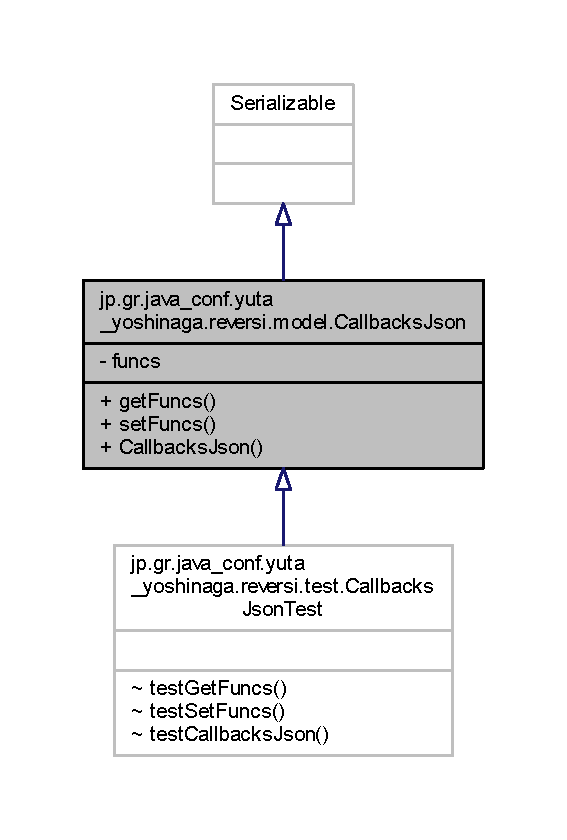
\includegraphics[width=272pt]{classjp_1_1gr_1_1java__conf_1_1yuta__yoshinaga_1_1reversi_1_1model_1_1_callbacks_json__inherit__graph}
\end{center}
\end{figure}


Collaboration diagram for jp.\+gr.\+java\+\_\+conf.\+yuta\+\_\+yoshinaga.\+reversi.\+model.\+Callbacks\+Json\+:
\nopagebreak
\begin{figure}[H]
\begin{center}
\leavevmode
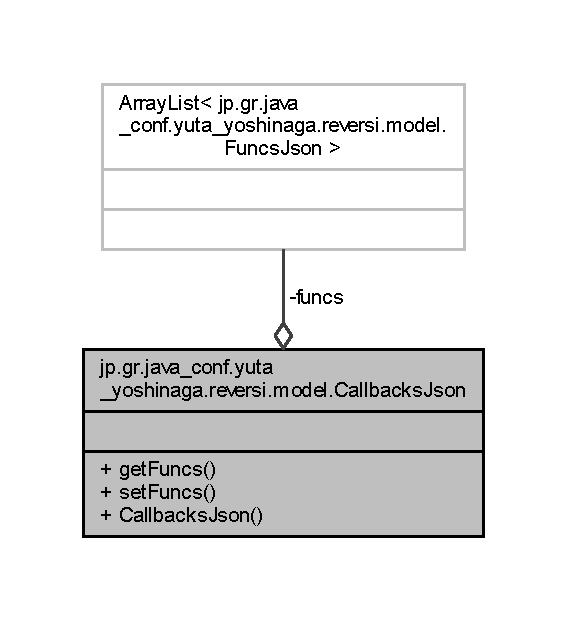
\includegraphics[width=340pt]{classjp_1_1gr_1_1java__conf_1_1yuta__yoshinaga_1_1reversi_1_1model_1_1_callbacks_json__coll__graph}
\end{center}
\end{figure}
\subsection*{Public Member Functions}
\begin{DoxyCompactItemize}
\item 
Array\+List$<$ \hyperlink{classjp_1_1gr_1_1java__conf_1_1yuta__yoshinaga_1_1reversi_1_1model_1_1_funcs_json}{Funcs\+Json} $>$ \hyperlink{classjp_1_1gr_1_1java__conf_1_1yuta__yoshinaga_1_1reversi_1_1model_1_1_callbacks_json_af9a62a3dbe6416793c01d7a0f69da2b1}{get\+Funcs} ()
\begin{DoxyCompactList}\small\item\em ゲッター \end{DoxyCompactList}\item 
void \hyperlink{classjp_1_1gr_1_1java__conf_1_1yuta__yoshinaga_1_1reversi_1_1model_1_1_callbacks_json_a6de1fc00c131167b4fe6231a660bdb6e}{set\+Funcs} (Array\+List$<$ \hyperlink{classjp_1_1gr_1_1java__conf_1_1yuta__yoshinaga_1_1reversi_1_1model_1_1_funcs_json}{Funcs\+Json} $>$ \hyperlink{classjp_1_1gr_1_1java__conf_1_1yuta__yoshinaga_1_1reversi_1_1model_1_1_callbacks_json_acbc23906e4e1cd6ff59a46ee2d7e1a85}{funcs})
\begin{DoxyCompactList}\small\item\em セッター \end{DoxyCompactList}\item 
\hyperlink{classjp_1_1gr_1_1java__conf_1_1yuta__yoshinaga_1_1reversi_1_1model_1_1_callbacks_json_acdc36faba755660c46ab3d1641d18e67}{Callbacks\+Json} ()
\begin{DoxyCompactList}\small\item\em コンストラクタ \end{DoxyCompactList}\end{DoxyCompactItemize}
\subsection*{Private Attributes}
\begin{DoxyCompactItemize}
\item 
\mbox{\Hypertarget{classjp_1_1gr_1_1java__conf_1_1yuta__yoshinaga_1_1reversi_1_1model_1_1_callbacks_json_acbc23906e4e1cd6ff59a46ee2d7e1a85}\label{classjp_1_1gr_1_1java__conf_1_1yuta__yoshinaga_1_1reversi_1_1model_1_1_callbacks_json_acbc23906e4e1cd6ff59a46ee2d7e1a85}} 
Array\+List$<$ \hyperlink{classjp_1_1gr_1_1java__conf_1_1yuta__yoshinaga_1_1reversi_1_1model_1_1_funcs_json}{Funcs\+Json} $>$ \hyperlink{classjp_1_1gr_1_1java__conf_1_1yuta__yoshinaga_1_1reversi_1_1model_1_1_callbacks_json_acbc23906e4e1cd6ff59a46ee2d7e1a85}{funcs}
\begin{DoxyCompactList}\small\item\em ファンクションズ \end{DoxyCompactList}\end{DoxyCompactItemize}


\subsection{Detailed Description}
コールバック\+J\+S\+O\+Nクラス 

Definition at line 28 of file Callbacks\+Json.\+java.



\subsection{Constructor \& Destructor Documentation}
\mbox{\Hypertarget{classjp_1_1gr_1_1java__conf_1_1yuta__yoshinaga_1_1reversi_1_1model_1_1_callbacks_json_acdc36faba755660c46ab3d1641d18e67}\label{classjp_1_1gr_1_1java__conf_1_1yuta__yoshinaga_1_1reversi_1_1model_1_1_callbacks_json_acdc36faba755660c46ab3d1641d18e67}} 
\index{jp\+::gr\+::java\+\_\+conf\+::yuta\+\_\+yoshinaga\+::reversi\+::model\+::\+Callbacks\+Json@{jp\+::gr\+::java\+\_\+conf\+::yuta\+\_\+yoshinaga\+::reversi\+::model\+::\+Callbacks\+Json}!Callbacks\+Json@{Callbacks\+Json}}
\index{Callbacks\+Json@{Callbacks\+Json}!jp\+::gr\+::java\+\_\+conf\+::yuta\+\_\+yoshinaga\+::reversi\+::model\+::\+Callbacks\+Json@{jp\+::gr\+::java\+\_\+conf\+::yuta\+\_\+yoshinaga\+::reversi\+::model\+::\+Callbacks\+Json}}
\subsubsection{\texorpdfstring{Callbacks\+Json()}{CallbacksJson()}}
{\footnotesize\ttfamily public jp.\+gr.\+java\+\_\+conf.\+yuta\+\_\+yoshinaga.\+reversi.\+model.\+Callbacks\+Json.\+Callbacks\+Json (\begin{DoxyParamCaption}{ }\end{DoxyParamCaption})}



コンストラクタ 

\begin{DoxyReturn}{Returns}
ありません 
\end{DoxyReturn}
\begin{DoxyAuthor}{Author}
Yuta Yoshinaga 
\end{DoxyAuthor}
\begin{DoxyDate}{Date}
2018.\+04.\+01 
\end{DoxyDate}


Definition at line 65 of file Callbacks\+Json.\+java.



\subsection{Member Function Documentation}
\mbox{\Hypertarget{classjp_1_1gr_1_1java__conf_1_1yuta__yoshinaga_1_1reversi_1_1model_1_1_callbacks_json_af9a62a3dbe6416793c01d7a0f69da2b1}\label{classjp_1_1gr_1_1java__conf_1_1yuta__yoshinaga_1_1reversi_1_1model_1_1_callbacks_json_af9a62a3dbe6416793c01d7a0f69da2b1}} 
\index{jp\+::gr\+::java\+\_\+conf\+::yuta\+\_\+yoshinaga\+::reversi\+::model\+::\+Callbacks\+Json@{jp\+::gr\+::java\+\_\+conf\+::yuta\+\_\+yoshinaga\+::reversi\+::model\+::\+Callbacks\+Json}!get\+Funcs@{get\+Funcs}}
\index{get\+Funcs@{get\+Funcs}!jp\+::gr\+::java\+\_\+conf\+::yuta\+\_\+yoshinaga\+::reversi\+::model\+::\+Callbacks\+Json@{jp\+::gr\+::java\+\_\+conf\+::yuta\+\_\+yoshinaga\+::reversi\+::model\+::\+Callbacks\+Json}}
\subsubsection{\texorpdfstring{get\+Funcs()}{getFuncs()}}
{\footnotesize\ttfamily Array\+List$<$ \hyperlink{classjp_1_1gr_1_1java__conf_1_1yuta__yoshinaga_1_1reversi_1_1model_1_1_funcs_json}{Funcs\+Json} $>$ jp.\+gr.\+java\+\_\+conf.\+yuta\+\_\+yoshinaga.\+reversi.\+model.\+Callbacks\+Json.\+get\+Funcs (\begin{DoxyParamCaption}{ }\end{DoxyParamCaption})}



ゲッター 

\begin{DoxyReturn}{Returns}
Array\+List$<$\+Funcs\+Json$>$ funcs 
\end{DoxyReturn}
\begin{DoxyAuthor}{Author}
Yuta Yoshinaga 
\end{DoxyAuthor}
\begin{DoxyDate}{Date}
2018.\+04.\+01 
\end{DoxyDate}


Definition at line 40 of file Callbacks\+Json.\+java.



Referenced by jp.\+gr.\+java\+\_\+conf.\+yuta\+\_\+yoshinaga.\+reversi.\+controller.\+Front\+Controller.\+Cur\+Col\+Msg(), jp.\+gr.\+java\+\_\+conf.\+yuta\+\_\+yoshinaga.\+reversi.\+controller.\+Front\+Controller.\+Cur\+Sts\+Msg(), jp.\+gr.\+java\+\_\+conf.\+yuta\+\_\+yoshinaga.\+reversi.\+controller.\+Front\+Controller.\+Draw\+Single(), jp.\+gr.\+java\+\_\+conf.\+yuta\+\_\+yoshinaga.\+reversi.\+controller.\+Front\+Controller.\+View\+Msg\+Dlg(), and jp.\+gr.\+java\+\_\+conf.\+yuta\+\_\+yoshinaga.\+reversi.\+controller.\+Front\+Controller.\+Wait().

Here is the caller graph for this function\+:
\nopagebreak
\begin{figure}[H]
\begin{center}
\leavevmode
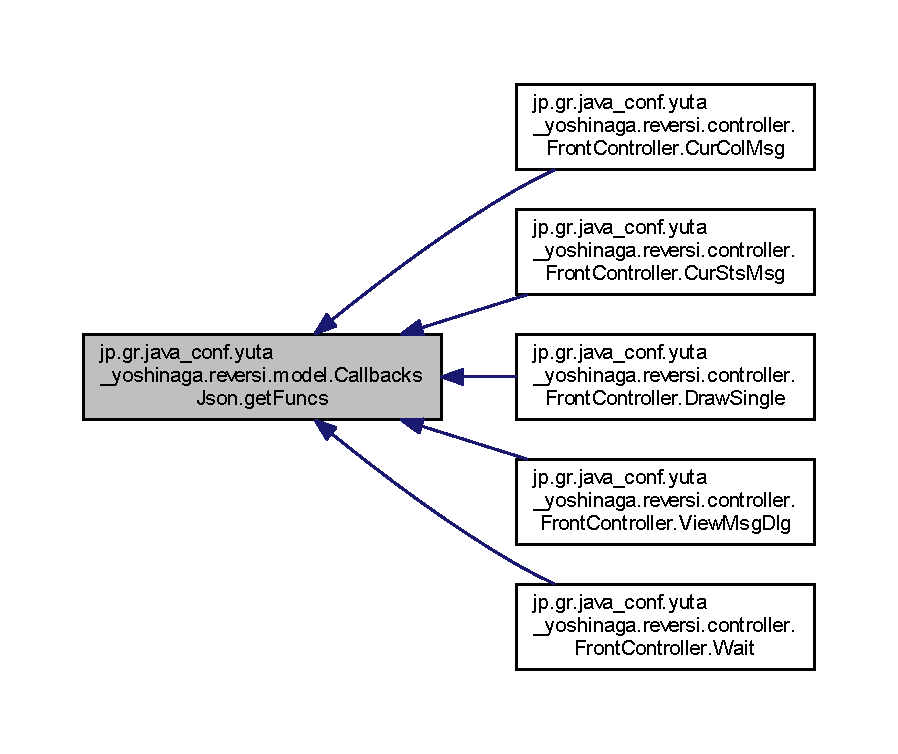
\includegraphics[width=350pt]{classjp_1_1gr_1_1java__conf_1_1yuta__yoshinaga_1_1reversi_1_1model_1_1_callbacks_json_af9a62a3dbe6416793c01d7a0f69da2b1_icgraph}
\end{center}
\end{figure}
\mbox{\Hypertarget{classjp_1_1gr_1_1java__conf_1_1yuta__yoshinaga_1_1reversi_1_1model_1_1_callbacks_json_a6de1fc00c131167b4fe6231a660bdb6e}\label{classjp_1_1gr_1_1java__conf_1_1yuta__yoshinaga_1_1reversi_1_1model_1_1_callbacks_json_a6de1fc00c131167b4fe6231a660bdb6e}} 
\index{jp\+::gr\+::java\+\_\+conf\+::yuta\+\_\+yoshinaga\+::reversi\+::model\+::\+Callbacks\+Json@{jp\+::gr\+::java\+\_\+conf\+::yuta\+\_\+yoshinaga\+::reversi\+::model\+::\+Callbacks\+Json}!set\+Funcs@{set\+Funcs}}
\index{set\+Funcs@{set\+Funcs}!jp\+::gr\+::java\+\_\+conf\+::yuta\+\_\+yoshinaga\+::reversi\+::model\+::\+Callbacks\+Json@{jp\+::gr\+::java\+\_\+conf\+::yuta\+\_\+yoshinaga\+::reversi\+::model\+::\+Callbacks\+Json}}
\subsubsection{\texorpdfstring{set\+Funcs()}{setFuncs()}}
{\footnotesize\ttfamily void jp.\+gr.\+java\+\_\+conf.\+yuta\+\_\+yoshinaga.\+reversi.\+model.\+Callbacks\+Json.\+set\+Funcs (\begin{DoxyParamCaption}\item[{Array\+List$<$ \hyperlink{classjp_1_1gr_1_1java__conf_1_1yuta__yoshinaga_1_1reversi_1_1model_1_1_funcs_json}{Funcs\+Json} $>$}]{funcs }\end{DoxyParamCaption})}



セッター 


\begin{DoxyParams}[1]{Parameters}
\mbox{\tt in}  & {\em Array\+List$<$\+Funcs\+Json$>$} & funcs \\
\hline
\end{DoxyParams}
\begin{DoxyReturn}{Returns}
ありません 
\end{DoxyReturn}
\begin{DoxyAuthor}{Author}
Yuta Yoshinaga 
\end{DoxyAuthor}
\begin{DoxyDate}{Date}
2018.\+04.\+01 
\end{DoxyDate}


Definition at line 53 of file Callbacks\+Json.\+java.



The documentation for this class was generated from the following file\+:\begin{DoxyCompactItemize}
\item 
jp/gr/java\+\_\+conf/yuta\+\_\+yoshinaga/reversi/model/\hyperlink{_callbacks_json_8java}{Callbacks\+Json.\+java}\end{DoxyCompactItemize}

\hypertarget{classjp_1_1gr_1_1java__conf_1_1yuta__yoshinaga_1_1reversi_1_1controller_1_1_front_controller}{}\section{jp.\+gr.\+java\+\_\+conf.\+yuta\+\_\+yoshinaga.\+reversi.\+controller.\+Front\+Controller Class Reference}
\label{classjp_1_1gr_1_1java__conf_1_1yuta__yoshinaga_1_1reversi_1_1controller_1_1_front_controller}\index{jp.\+gr.\+java\+\_\+conf.\+yuta\+\_\+yoshinaga.\+reversi.\+controller.\+Front\+Controller@{jp.\+gr.\+java\+\_\+conf.\+yuta\+\_\+yoshinaga.\+reversi.\+controller.\+Front\+Controller}}


Servlet implementation class \hyperlink{classjp_1_1gr_1_1java__conf_1_1yuta__yoshinaga_1_1reversi_1_1controller_1_1_front_controller}{Front\+Controller}.  




Inheritance diagram for jp.\+gr.\+java\+\_\+conf.\+yuta\+\_\+yoshinaga.\+reversi.\+controller.\+Front\+Controller\+:\nopagebreak
\begin{figure}[H]
\begin{center}
\leavevmode
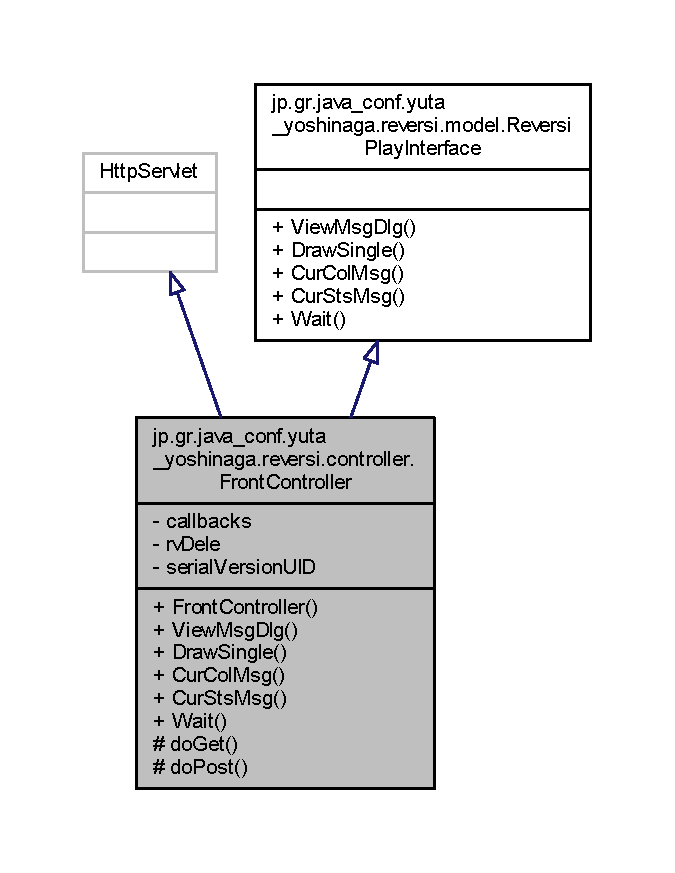
\includegraphics[width=324pt]{classjp_1_1gr_1_1java__conf_1_1yuta__yoshinaga_1_1reversi_1_1controller_1_1_front_controller__inherit__graph}
\end{center}
\end{figure}


Collaboration diagram for jp.\+gr.\+java\+\_\+conf.\+yuta\+\_\+yoshinaga.\+reversi.\+controller.\+Front\+Controller\+:\nopagebreak
\begin{figure}[H]
\begin{center}
\leavevmode
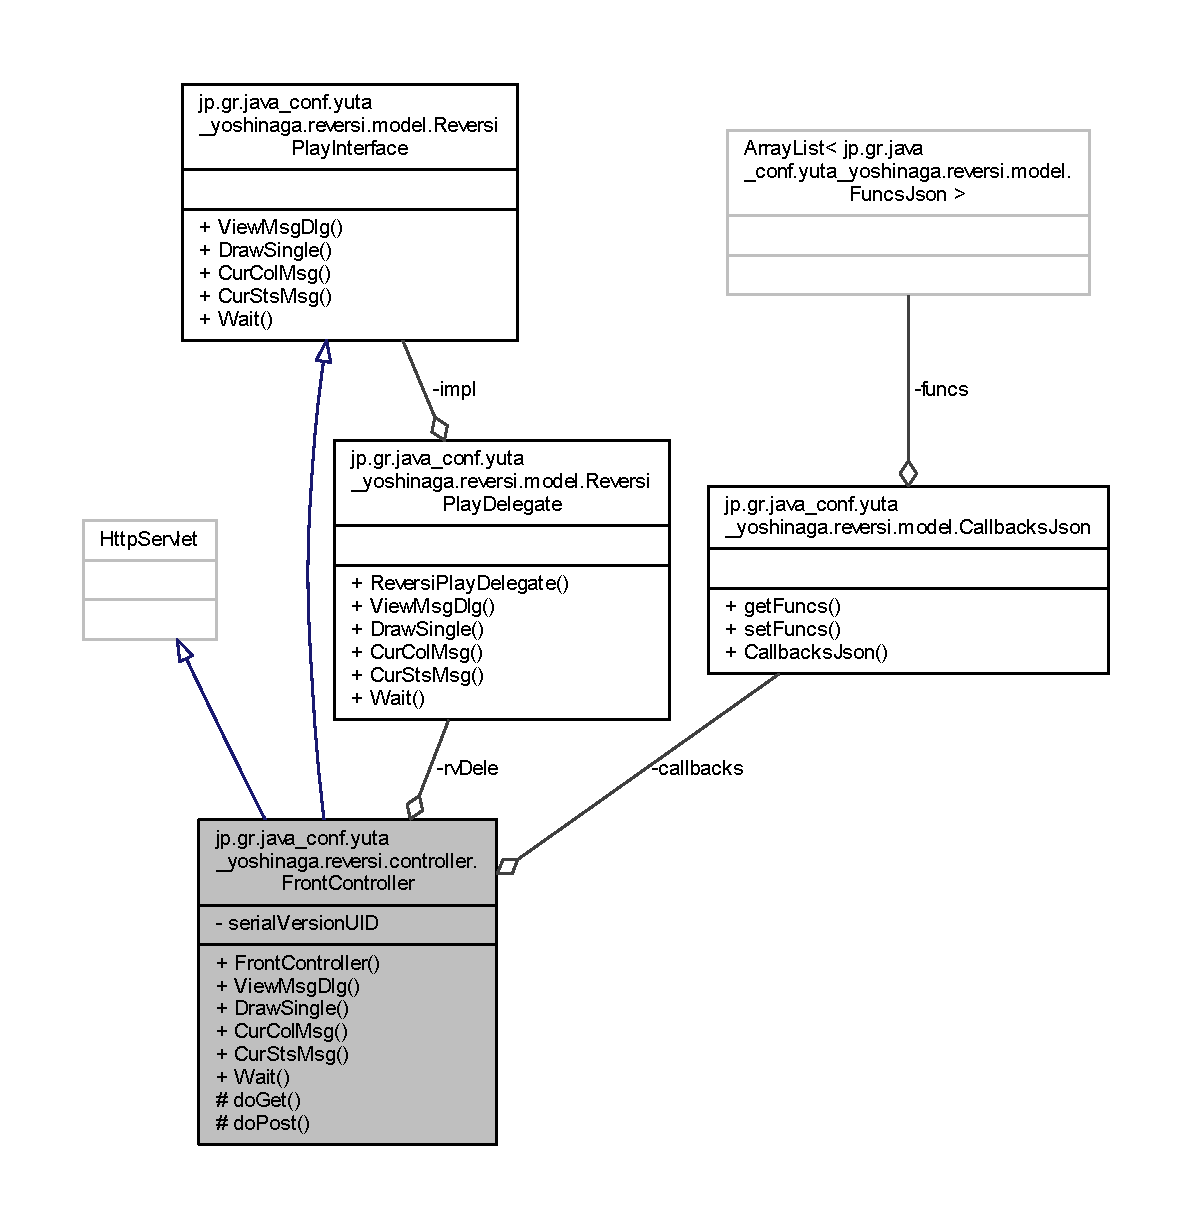
\includegraphics[width=350pt]{classjp_1_1gr_1_1java__conf_1_1yuta__yoshinaga_1_1reversi_1_1controller_1_1_front_controller__coll__graph}
\end{center}
\end{figure}
\subsection*{Public Member Functions}
\begin{DoxyCompactItemize}
\item 
\hyperlink{classjp_1_1gr_1_1java__conf_1_1yuta__yoshinaga_1_1reversi_1_1controller_1_1_front_controller_a918d736b7b4d8672076c15f8ca05075c}{Front\+Controller} ()
\begin{DoxyCompactList}\small\item\em コンストラクタ \end{DoxyCompactList}\item 
void \hyperlink{classjp_1_1gr_1_1java__conf_1_1yuta__yoshinaga_1_1reversi_1_1controller_1_1_front_controller_a03f8b3b1b7991cfb075f8708d4041ddb}{View\+Msg\+Dlg} (String title, String msg)
\begin{DoxyCompactList}\small\item\em メッセージダイアログ \end{DoxyCompactList}\item 
void \hyperlink{classjp_1_1gr_1_1java__conf_1_1yuta__yoshinaga_1_1reversi_1_1controller_1_1_front_controller_acf079ebc5949ce36b15c56158c9b9cfa}{Draw\+Single} (int y, int x, int sts, int bk, String text)
\begin{DoxyCompactList}\small\item\em 1マス描画 \end{DoxyCompactList}\item 
void \hyperlink{classjp_1_1gr_1_1java__conf_1_1yuta__yoshinaga_1_1reversi_1_1controller_1_1_front_controller_ac49c44c8bb767770364c52164b699110}{Cur\+Col\+Msg} (String text)
\begin{DoxyCompactList}\small\item\em 現在の色メッセージ \end{DoxyCompactList}\item 
void \hyperlink{classjp_1_1gr_1_1java__conf_1_1yuta__yoshinaga_1_1reversi_1_1controller_1_1_front_controller_a49315230e704778721afb73c59e14d88}{Cur\+Sts\+Msg} (String text)
\begin{DoxyCompactList}\small\item\em 現在のステータスメッセージ \end{DoxyCompactList}\item 
void \hyperlink{classjp_1_1gr_1_1java__conf_1_1yuta__yoshinaga_1_1reversi_1_1controller_1_1_front_controller_af513d1ccfca9fc00f93fb650f1f08b05}{Wait} (int time)
\begin{DoxyCompactList}\small\item\em ウェイト \end{DoxyCompactList}\end{DoxyCompactItemize}
\subsection*{Protected Member Functions}
\begin{DoxyCompactItemize}
\item 
void \hyperlink{classjp_1_1gr_1_1java__conf_1_1yuta__yoshinaga_1_1reversi_1_1controller_1_1_front_controller_a2f0d63da6e6fc17d2ecf2695af6f8d99}{do\+Post} (Http\+Servlet\+Request request, Http\+Servlet\+Response response)  throws Servlet\+Exception, I\+O\+Exception 
\begin{DoxyCompactList}\small\item\em P\+O\+ST. \end{DoxyCompactList}\end{DoxyCompactItemize}
\subsection*{Private Attributes}
\begin{DoxyCompactItemize}
\item 
\mbox{\Hypertarget{classjp_1_1gr_1_1java__conf_1_1yuta__yoshinaga_1_1reversi_1_1controller_1_1_front_controller_aba15286819435469622375192358dee7}\label{classjp_1_1gr_1_1java__conf_1_1yuta__yoshinaga_1_1reversi_1_1controller_1_1_front_controller_aba15286819435469622375192358dee7}} 
\hyperlink{classjp_1_1gr_1_1java__conf_1_1yuta__yoshinaga_1_1reversi_1_1model_1_1_callbacks_json}{Callbacks\+Json} {\bfseries callbacks} = null
\item 
\mbox{\Hypertarget{classjp_1_1gr_1_1java__conf_1_1yuta__yoshinaga_1_1reversi_1_1controller_1_1_front_controller_a582bcd1cbb69aaf686182d85dbd21f2d}\label{classjp_1_1gr_1_1java__conf_1_1yuta__yoshinaga_1_1reversi_1_1controller_1_1_front_controller_a582bcd1cbb69aaf686182d85dbd21f2d}} 
\hyperlink{classjp_1_1gr_1_1java__conf_1_1yuta__yoshinaga_1_1reversi_1_1model_1_1_reversi_play_delegate}{Reversi\+Play\+Delegate} {\bfseries rv\+Dele} = null
\end{DoxyCompactItemize}
\subsection*{Static Private Attributes}
\begin{DoxyCompactItemize}
\item 
\mbox{\Hypertarget{classjp_1_1gr_1_1java__conf_1_1yuta__yoshinaga_1_1reversi_1_1controller_1_1_front_controller_a42e40239dd4f246bd1524cdb08ca41af}\label{classjp_1_1gr_1_1java__conf_1_1yuta__yoshinaga_1_1reversi_1_1controller_1_1_front_controller_a42e40239dd4f246bd1524cdb08ca41af}} 
static final long {\bfseries serial\+Version\+U\+ID} = 1L
\end{DoxyCompactItemize}


\subsection{Detailed Description}
Servlet implementation class \hyperlink{classjp_1_1gr_1_1java__conf_1_1yuta__yoshinaga_1_1reversi_1_1controller_1_1_front_controller}{Front\+Controller}. 

Definition at line 44 of file Front\+Controller.\+java.



\subsection{Constructor \& Destructor Documentation}
\mbox{\Hypertarget{classjp_1_1gr_1_1java__conf_1_1yuta__yoshinaga_1_1reversi_1_1controller_1_1_front_controller_a918d736b7b4d8672076c15f8ca05075c}\label{classjp_1_1gr_1_1java__conf_1_1yuta__yoshinaga_1_1reversi_1_1controller_1_1_front_controller_a918d736b7b4d8672076c15f8ca05075c}} 
\index{jp\+::gr\+::java\+\_\+conf\+::yuta\+\_\+yoshinaga\+::reversi\+::controller\+::\+Front\+Controller@{jp\+::gr\+::java\+\_\+conf\+::yuta\+\_\+yoshinaga\+::reversi\+::controller\+::\+Front\+Controller}!Front\+Controller@{Front\+Controller}}
\index{Front\+Controller@{Front\+Controller}!jp\+::gr\+::java\+\_\+conf\+::yuta\+\_\+yoshinaga\+::reversi\+::controller\+::\+Front\+Controller@{jp\+::gr\+::java\+\_\+conf\+::yuta\+\_\+yoshinaga\+::reversi\+::controller\+::\+Front\+Controller}}
\subsubsection{\texorpdfstring{Front\+Controller()}{FrontController()}}
{\footnotesize\ttfamily public jp.\+gr.\+java\+\_\+conf.\+yuta\+\_\+yoshinaga.\+reversi.\+controller.\+Front\+Controller.\+Front\+Controller (\begin{DoxyParamCaption}{ }\end{DoxyParamCaption})}



コンストラクタ 

\begin{DoxyReturn}{Returns}
ありません 
\end{DoxyReturn}
\begin{DoxyAuthor}{Author}
Yuta Yoshinaga 
\end{DoxyAuthor}
\begin{DoxyDate}{Date}
2018.\+04.\+01 
\end{DoxyDate}
\begin{DoxySeeAlso}{See also}
Http\+Servlet\+::\+Http\+Servlet() 
\end{DoxySeeAlso}


Definition at line 58 of file Front\+Controller.\+java.



\subsection{Member Function Documentation}
\mbox{\Hypertarget{classjp_1_1gr_1_1java__conf_1_1yuta__yoshinaga_1_1reversi_1_1controller_1_1_front_controller_ac49c44c8bb767770364c52164b699110}\label{classjp_1_1gr_1_1java__conf_1_1yuta__yoshinaga_1_1reversi_1_1controller_1_1_front_controller_ac49c44c8bb767770364c52164b699110}} 
\index{jp\+::gr\+::java\+\_\+conf\+::yuta\+\_\+yoshinaga\+::reversi\+::controller\+::\+Front\+Controller@{jp\+::gr\+::java\+\_\+conf\+::yuta\+\_\+yoshinaga\+::reversi\+::controller\+::\+Front\+Controller}!Cur\+Col\+Msg@{Cur\+Col\+Msg}}
\index{Cur\+Col\+Msg@{Cur\+Col\+Msg}!jp\+::gr\+::java\+\_\+conf\+::yuta\+\_\+yoshinaga\+::reversi\+::controller\+::\+Front\+Controller@{jp\+::gr\+::java\+\_\+conf\+::yuta\+\_\+yoshinaga\+::reversi\+::controller\+::\+Front\+Controller}}
\subsubsection{\texorpdfstring{Cur\+Col\+Msg()}{CurColMsg()}}
{\footnotesize\ttfamily void jp.\+gr.\+java\+\_\+conf.\+yuta\+\_\+yoshinaga.\+reversi.\+controller.\+Front\+Controller.\+Cur\+Col\+Msg (\begin{DoxyParamCaption}\item[{String}]{text }\end{DoxyParamCaption})}



現在の色メッセージ 


\begin{DoxyParams}[1]{Parameters}
\mbox{\tt in}  & {\em String} & text テキスト \\
\hline
\end{DoxyParams}
\begin{DoxyReturn}{Returns}
ありません 
\end{DoxyReturn}
\begin{DoxyAuthor}{Author}
Yuta Yoshinaga 
\end{DoxyAuthor}
\begin{DoxyDate}{Date}
2018.\+04.\+01 
\end{DoxyDate}


Implements \hyperlink{interfacejp_1_1gr_1_1java__conf_1_1yuta__yoshinaga_1_1reversi_1_1model_1_1_reversi_play_interface_a73764de038c314fd103a91d402049a0c}{jp.\+gr.\+java\+\_\+conf.\+yuta\+\_\+yoshinaga.\+reversi.\+model.\+Reversi\+Play\+Interface}.



Definition at line 184 of file Front\+Controller.\+java.

Here is the call graph for this function\+:\nopagebreak
\begin{figure}[H]
\begin{center}
\leavevmode
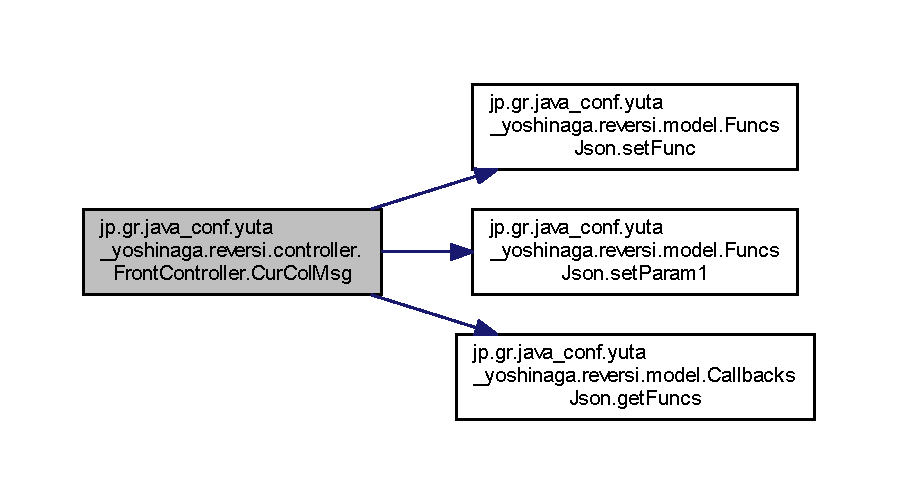
\includegraphics[width=350pt]{classjp_1_1gr_1_1java__conf_1_1yuta__yoshinaga_1_1reversi_1_1controller_1_1_front_controller_ac49c44c8bb767770364c52164b699110_cgraph}
\end{center}
\end{figure}
\mbox{\Hypertarget{classjp_1_1gr_1_1java__conf_1_1yuta__yoshinaga_1_1reversi_1_1controller_1_1_front_controller_a49315230e704778721afb73c59e14d88}\label{classjp_1_1gr_1_1java__conf_1_1yuta__yoshinaga_1_1reversi_1_1controller_1_1_front_controller_a49315230e704778721afb73c59e14d88}} 
\index{jp\+::gr\+::java\+\_\+conf\+::yuta\+\_\+yoshinaga\+::reversi\+::controller\+::\+Front\+Controller@{jp\+::gr\+::java\+\_\+conf\+::yuta\+\_\+yoshinaga\+::reversi\+::controller\+::\+Front\+Controller}!Cur\+Sts\+Msg@{Cur\+Sts\+Msg}}
\index{Cur\+Sts\+Msg@{Cur\+Sts\+Msg}!jp\+::gr\+::java\+\_\+conf\+::yuta\+\_\+yoshinaga\+::reversi\+::controller\+::\+Front\+Controller@{jp\+::gr\+::java\+\_\+conf\+::yuta\+\_\+yoshinaga\+::reversi\+::controller\+::\+Front\+Controller}}
\subsubsection{\texorpdfstring{Cur\+Sts\+Msg()}{CurStsMsg()}}
{\footnotesize\ttfamily void jp.\+gr.\+java\+\_\+conf.\+yuta\+\_\+yoshinaga.\+reversi.\+controller.\+Front\+Controller.\+Cur\+Sts\+Msg (\begin{DoxyParamCaption}\item[{String}]{text }\end{DoxyParamCaption})}



現在のステータスメッセージ 


\begin{DoxyParams}[1]{Parameters}
\mbox{\tt in}  & {\em String} & text テキスト \\
\hline
\end{DoxyParams}
\begin{DoxyReturn}{Returns}
ありません 
\end{DoxyReturn}
\begin{DoxyAuthor}{Author}
Yuta Yoshinaga 
\end{DoxyAuthor}
\begin{DoxyDate}{Date}
2018.\+04.\+01 
\end{DoxyDate}


Implements \hyperlink{interfacejp_1_1gr_1_1java__conf_1_1yuta__yoshinaga_1_1reversi_1_1model_1_1_reversi_play_interface_ad812b3735df400b42916b15e5c3ff9db}{jp.\+gr.\+java\+\_\+conf.\+yuta\+\_\+yoshinaga.\+reversi.\+model.\+Reversi\+Play\+Interface}.



Definition at line 202 of file Front\+Controller.\+java.

Here is the call graph for this function\+:\nopagebreak
\begin{figure}[H]
\begin{center}
\leavevmode
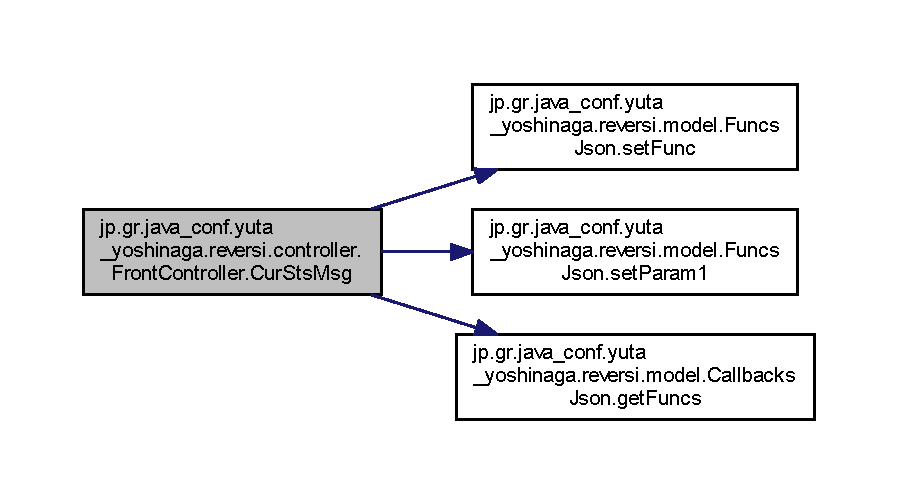
\includegraphics[width=350pt]{classjp_1_1gr_1_1java__conf_1_1yuta__yoshinaga_1_1reversi_1_1controller_1_1_front_controller_a49315230e704778721afb73c59e14d88_cgraph}
\end{center}
\end{figure}
\mbox{\Hypertarget{classjp_1_1gr_1_1java__conf_1_1yuta__yoshinaga_1_1reversi_1_1controller_1_1_front_controller_a2f0d63da6e6fc17d2ecf2695af6f8d99}\label{classjp_1_1gr_1_1java__conf_1_1yuta__yoshinaga_1_1reversi_1_1controller_1_1_front_controller_a2f0d63da6e6fc17d2ecf2695af6f8d99}} 
\index{jp\+::gr\+::java\+\_\+conf\+::yuta\+\_\+yoshinaga\+::reversi\+::controller\+::\+Front\+Controller@{jp\+::gr\+::java\+\_\+conf\+::yuta\+\_\+yoshinaga\+::reversi\+::controller\+::\+Front\+Controller}!do\+Post@{do\+Post}}
\index{do\+Post@{do\+Post}!jp\+::gr\+::java\+\_\+conf\+::yuta\+\_\+yoshinaga\+::reversi\+::controller\+::\+Front\+Controller@{jp\+::gr\+::java\+\_\+conf\+::yuta\+\_\+yoshinaga\+::reversi\+::controller\+::\+Front\+Controller}}
\subsubsection{\texorpdfstring{do\+Post()}{doPost()}}
{\footnotesize\ttfamily protected void jp.\+gr.\+java\+\_\+conf.\+yuta\+\_\+yoshinaga.\+reversi.\+controller.\+Front\+Controller.\+do\+Post (\begin{DoxyParamCaption}\item[{Http\+Servlet\+Request}]{request,  }\item[{Http\+Servlet\+Response}]{response }\end{DoxyParamCaption}) throws Servlet\+Exception, I\+O\+Exception\hspace{0.3cm}{\ttfamily [protected]}}



P\+O\+ST. 


\begin{DoxyParams}[1]{Parameters}
\mbox{\tt in}  & {\em Http\+Servlet\+Request} & request \\
\hline
\mbox{\tt in,out}  & {\em Http\+Servlet\+Response} & response \\
\hline
\end{DoxyParams}
\begin{DoxyReturn}{Returns}
ありません 
\end{DoxyReturn}
\begin{DoxyAuthor}{Author}
Yuta Yoshinaga 
\end{DoxyAuthor}
\begin{DoxyDate}{Date}
2018.\+04.\+01 
\end{DoxyDate}
\begin{DoxySeeAlso}{See also}
Http\+Servlet\+::do\+Post(\+Http\+Servlet\+Request request, Http\+Servlet\+Response response) 
\end{DoxySeeAlso}


Definition at line 75 of file Front\+Controller.\+java.

Here is the call graph for this function\+:
\nopagebreak
\begin{figure}[H]
\begin{center}
\leavevmode
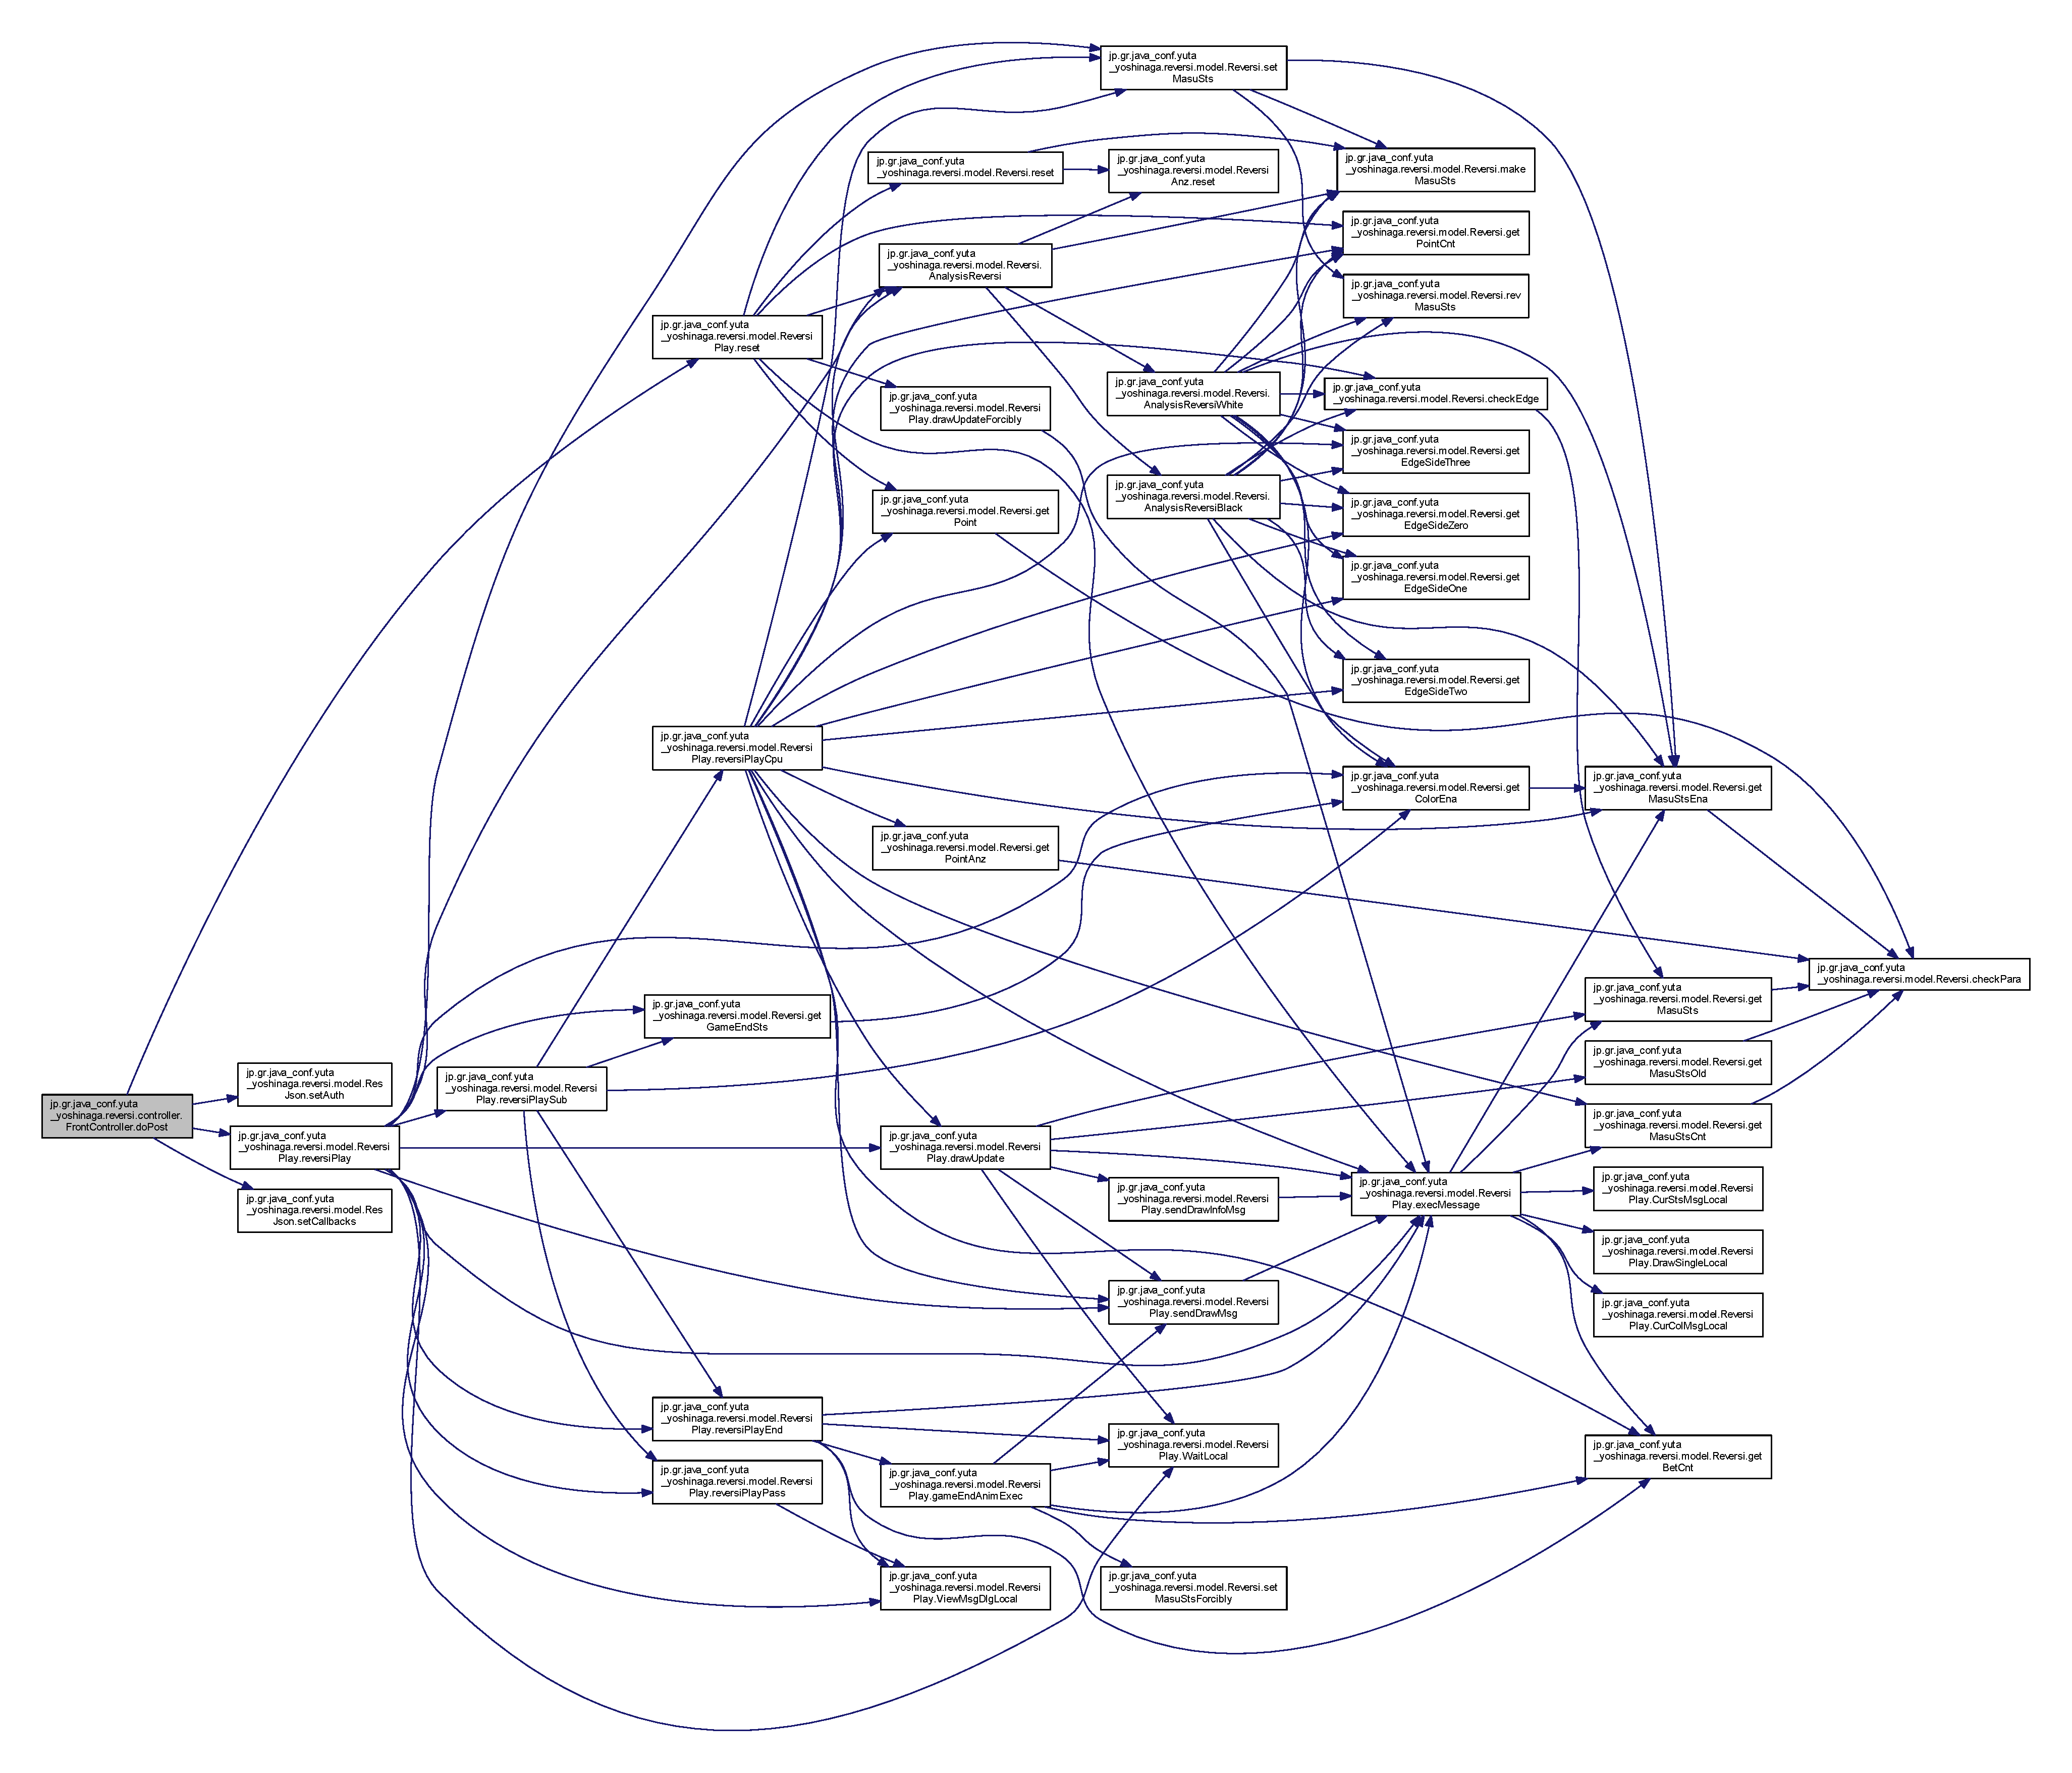
\includegraphics[width=350pt]{classjp_1_1gr_1_1java__conf_1_1yuta__yoshinaga_1_1reversi_1_1controller_1_1_front_controller_a2f0d63da6e6fc17d2ecf2695af6f8d99_cgraph}
\end{center}
\end{figure}
\mbox{\Hypertarget{classjp_1_1gr_1_1java__conf_1_1yuta__yoshinaga_1_1reversi_1_1controller_1_1_front_controller_acf079ebc5949ce36b15c56158c9b9cfa}\label{classjp_1_1gr_1_1java__conf_1_1yuta__yoshinaga_1_1reversi_1_1controller_1_1_front_controller_acf079ebc5949ce36b15c56158c9b9cfa}} 
\index{jp\+::gr\+::java\+\_\+conf\+::yuta\+\_\+yoshinaga\+::reversi\+::controller\+::\+Front\+Controller@{jp\+::gr\+::java\+\_\+conf\+::yuta\+\_\+yoshinaga\+::reversi\+::controller\+::\+Front\+Controller}!Draw\+Single@{Draw\+Single}}
\index{Draw\+Single@{Draw\+Single}!jp\+::gr\+::java\+\_\+conf\+::yuta\+\_\+yoshinaga\+::reversi\+::controller\+::\+Front\+Controller@{jp\+::gr\+::java\+\_\+conf\+::yuta\+\_\+yoshinaga\+::reversi\+::controller\+::\+Front\+Controller}}
\subsubsection{\texorpdfstring{Draw\+Single()}{DrawSingle()}}
{\footnotesize\ttfamily void jp.\+gr.\+java\+\_\+conf.\+yuta\+\_\+yoshinaga.\+reversi.\+controller.\+Front\+Controller.\+Draw\+Single (\begin{DoxyParamCaption}\item[{int}]{y,  }\item[{int}]{x,  }\item[{int}]{sts,  }\item[{int}]{bk,  }\item[{String}]{text }\end{DoxyParamCaption})}



1マス描画 


\begin{DoxyParams}[1]{Parameters}
\mbox{\tt in}  & {\em int} & y Y座標 \\
\hline
\mbox{\tt in}  & {\em int} & x X座標 \\
\hline
\mbox{\tt in}  & {\em int} & sts ステータス \\
\hline
\mbox{\tt in}  & {\em int} & bk 背景 \\
\hline
\mbox{\tt in}  & {\em String} & text テキスト \\
\hline
\end{DoxyParams}
\begin{DoxyReturn}{Returns}
ありません 
\end{DoxyReturn}
\begin{DoxyAuthor}{Author}
Yuta Yoshinaga 
\end{DoxyAuthor}
\begin{DoxyDate}{Date}
2018.\+04.\+01 
\end{DoxyDate}


Implements \hyperlink{interfacejp_1_1gr_1_1java__conf_1_1yuta__yoshinaga_1_1reversi_1_1model_1_1_reversi_play_interface_a6b51f93e409bbc76092e12a68c6fe710}{jp.\+gr.\+java\+\_\+conf.\+yuta\+\_\+yoshinaga.\+reversi.\+model.\+Reversi\+Play\+Interface}.



Definition at line 162 of file Front\+Controller.\+java.

Here is the call graph for this function\+:
\nopagebreak
\begin{figure}[H]
\begin{center}
\leavevmode
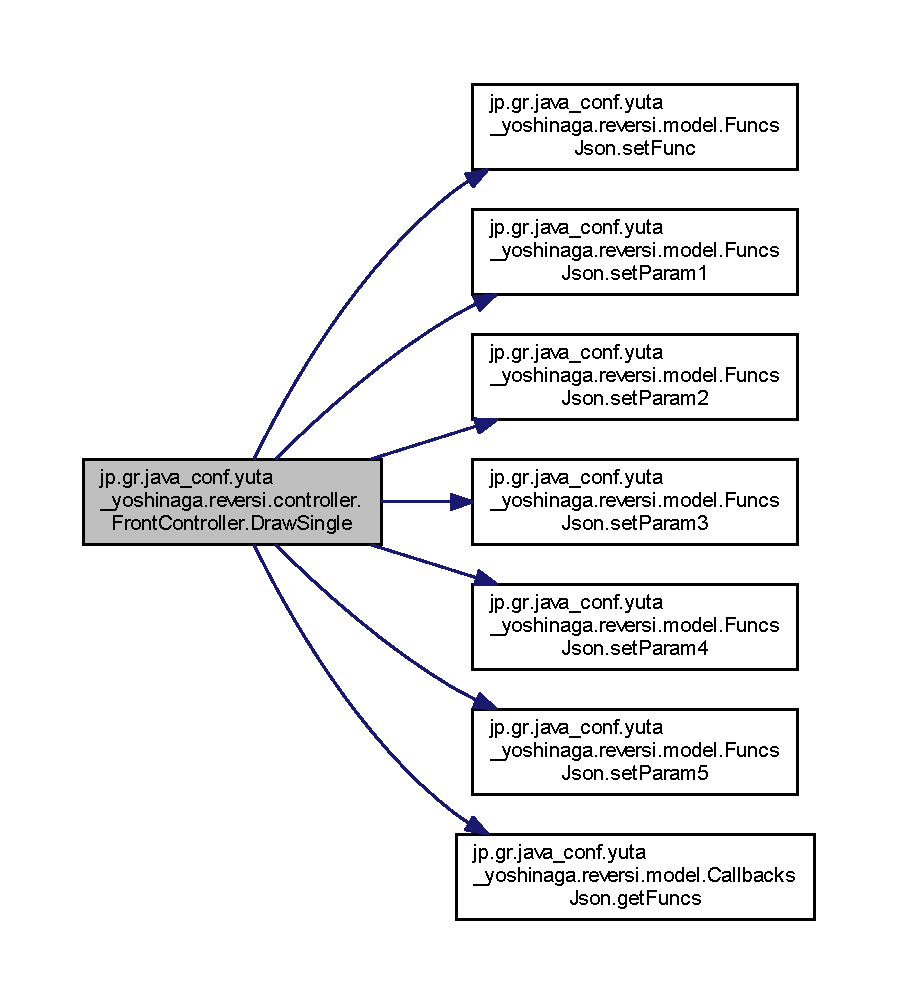
\includegraphics[width=350pt]{classjp_1_1gr_1_1java__conf_1_1yuta__yoshinaga_1_1reversi_1_1controller_1_1_front_controller_acf079ebc5949ce36b15c56158c9b9cfa_cgraph}
\end{center}
\end{figure}
\mbox{\Hypertarget{classjp_1_1gr_1_1java__conf_1_1yuta__yoshinaga_1_1reversi_1_1controller_1_1_front_controller_a03f8b3b1b7991cfb075f8708d4041ddb}\label{classjp_1_1gr_1_1java__conf_1_1yuta__yoshinaga_1_1reversi_1_1controller_1_1_front_controller_a03f8b3b1b7991cfb075f8708d4041ddb}} 
\index{jp\+::gr\+::java\+\_\+conf\+::yuta\+\_\+yoshinaga\+::reversi\+::controller\+::\+Front\+Controller@{jp\+::gr\+::java\+\_\+conf\+::yuta\+\_\+yoshinaga\+::reversi\+::controller\+::\+Front\+Controller}!View\+Msg\+Dlg@{View\+Msg\+Dlg}}
\index{View\+Msg\+Dlg@{View\+Msg\+Dlg}!jp\+::gr\+::java\+\_\+conf\+::yuta\+\_\+yoshinaga\+::reversi\+::controller\+::\+Front\+Controller@{jp\+::gr\+::java\+\_\+conf\+::yuta\+\_\+yoshinaga\+::reversi\+::controller\+::\+Front\+Controller}}
\subsubsection{\texorpdfstring{View\+Msg\+Dlg()}{ViewMsgDlg()}}
{\footnotesize\ttfamily void jp.\+gr.\+java\+\_\+conf.\+yuta\+\_\+yoshinaga.\+reversi.\+controller.\+Front\+Controller.\+View\+Msg\+Dlg (\begin{DoxyParamCaption}\item[{String}]{title,  }\item[{String}]{msg }\end{DoxyParamCaption})}



メッセージダイアログ 


\begin{DoxyParams}[1]{Parameters}
\mbox{\tt in}  & {\em String} & title タイトル \\
\hline
\mbox{\tt in}  & {\em String} & msg メッセージ \\
\hline
\end{DoxyParams}
\begin{DoxyReturn}{Returns}
ありません 
\end{DoxyReturn}
\begin{DoxyAuthor}{Author}
Yuta Yoshinaga 
\end{DoxyAuthor}
\begin{DoxyDate}{Date}
2018.\+04.\+01 
\end{DoxyDate}


Implements \hyperlink{interfacejp_1_1gr_1_1java__conf_1_1yuta__yoshinaga_1_1reversi_1_1model_1_1_reversi_play_interface_a189301a8c066e9421a26d1f2df95b56e}{jp.\+gr.\+java\+\_\+conf.\+yuta\+\_\+yoshinaga.\+reversi.\+model.\+Reversi\+Play\+Interface}.



Definition at line 139 of file Front\+Controller.\+java.

Here is the call graph for this function\+:
\nopagebreak
\begin{figure}[H]
\begin{center}
\leavevmode
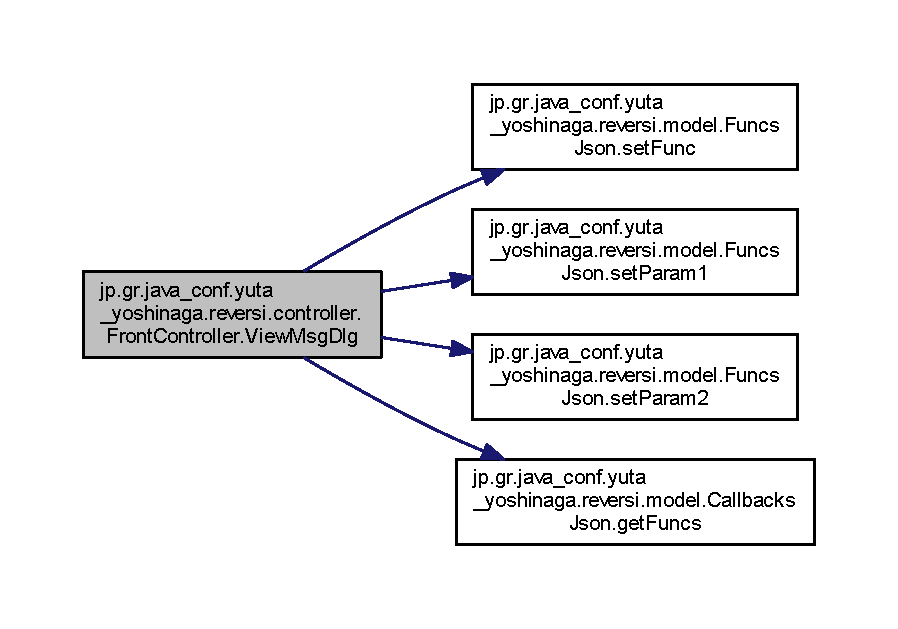
\includegraphics[width=350pt]{classjp_1_1gr_1_1java__conf_1_1yuta__yoshinaga_1_1reversi_1_1controller_1_1_front_controller_a03f8b3b1b7991cfb075f8708d4041ddb_cgraph}
\end{center}
\end{figure}
\mbox{\Hypertarget{classjp_1_1gr_1_1java__conf_1_1yuta__yoshinaga_1_1reversi_1_1controller_1_1_front_controller_af513d1ccfca9fc00f93fb650f1f08b05}\label{classjp_1_1gr_1_1java__conf_1_1yuta__yoshinaga_1_1reversi_1_1controller_1_1_front_controller_af513d1ccfca9fc00f93fb650f1f08b05}} 
\index{jp\+::gr\+::java\+\_\+conf\+::yuta\+\_\+yoshinaga\+::reversi\+::controller\+::\+Front\+Controller@{jp\+::gr\+::java\+\_\+conf\+::yuta\+\_\+yoshinaga\+::reversi\+::controller\+::\+Front\+Controller}!Wait@{Wait}}
\index{Wait@{Wait}!jp\+::gr\+::java\+\_\+conf\+::yuta\+\_\+yoshinaga\+::reversi\+::controller\+::\+Front\+Controller@{jp\+::gr\+::java\+\_\+conf\+::yuta\+\_\+yoshinaga\+::reversi\+::controller\+::\+Front\+Controller}}
\subsubsection{\texorpdfstring{Wait()}{Wait()}}
{\footnotesize\ttfamily void jp.\+gr.\+java\+\_\+conf.\+yuta\+\_\+yoshinaga.\+reversi.\+controller.\+Front\+Controller.\+Wait (\begin{DoxyParamCaption}\item[{int}]{time }\end{DoxyParamCaption})}



ウェイト 


\begin{DoxyParams}[1]{Parameters}
\mbox{\tt in}  & {\em int} & time ウェイト時間(msec) \\
\hline
\end{DoxyParams}
\begin{DoxyReturn}{Returns}
ありません 
\end{DoxyReturn}
\begin{DoxyAuthor}{Author}
Yuta Yoshinaga 
\end{DoxyAuthor}
\begin{DoxyDate}{Date}
2018.\+04.\+01 
\end{DoxyDate}


Implements \hyperlink{interfacejp_1_1gr_1_1java__conf_1_1yuta__yoshinaga_1_1reversi_1_1model_1_1_reversi_play_interface_abd7fc4193840e8c7bdf95bc538e1b649}{jp.\+gr.\+java\+\_\+conf.\+yuta\+\_\+yoshinaga.\+reversi.\+model.\+Reversi\+Play\+Interface}.



Definition at line 220 of file Front\+Controller.\+java.

Here is the call graph for this function\+:
\nopagebreak
\begin{figure}[H]
\begin{center}
\leavevmode
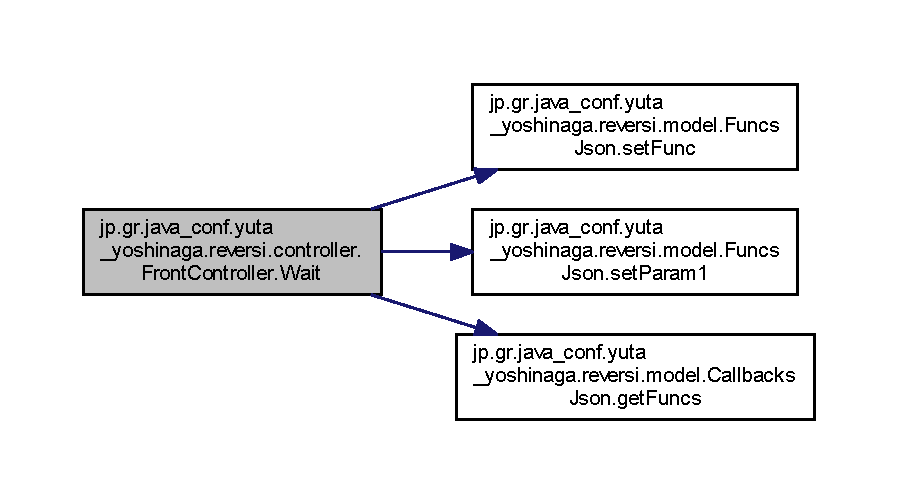
\includegraphics[width=350pt]{classjp_1_1gr_1_1java__conf_1_1yuta__yoshinaga_1_1reversi_1_1controller_1_1_front_controller_af513d1ccfca9fc00f93fb650f1f08b05_cgraph}
\end{center}
\end{figure}


The documentation for this class was generated from the following file\+:\begin{DoxyCompactItemize}
\item 
jp/gr/java\+\_\+conf/yuta\+\_\+yoshinaga/reversi/controller/\hyperlink{_front_controller_8java}{Front\+Controller.\+java}\end{DoxyCompactItemize}

\hypertarget{classjp_1_1gr_1_1java__conf_1_1yuta__yoshinaga_1_1reversi_1_1model_1_1_funcs_json}{}\section{jp.\+gr.\+java\+\_\+conf.\+yuta\+\_\+yoshinaga.\+reversi.\+model.\+Funcs\+Json Class Reference}
\label{classjp_1_1gr_1_1java__conf_1_1yuta__yoshinaga_1_1reversi_1_1model_1_1_funcs_json}\index{jp.\+gr.\+java\+\_\+conf.\+yuta\+\_\+yoshinaga.\+reversi.\+model.\+Funcs\+Json@{jp.\+gr.\+java\+\_\+conf.\+yuta\+\_\+yoshinaga.\+reversi.\+model.\+Funcs\+Json}}


ファンクション\+J\+S\+O\+Nクラス  




Inheritance diagram for jp.\+gr.\+java\+\_\+conf.\+yuta\+\_\+yoshinaga.\+reversi.\+model.\+Funcs\+Json\+:
\nopagebreak
\begin{figure}[H]
\begin{center}
\leavevmode
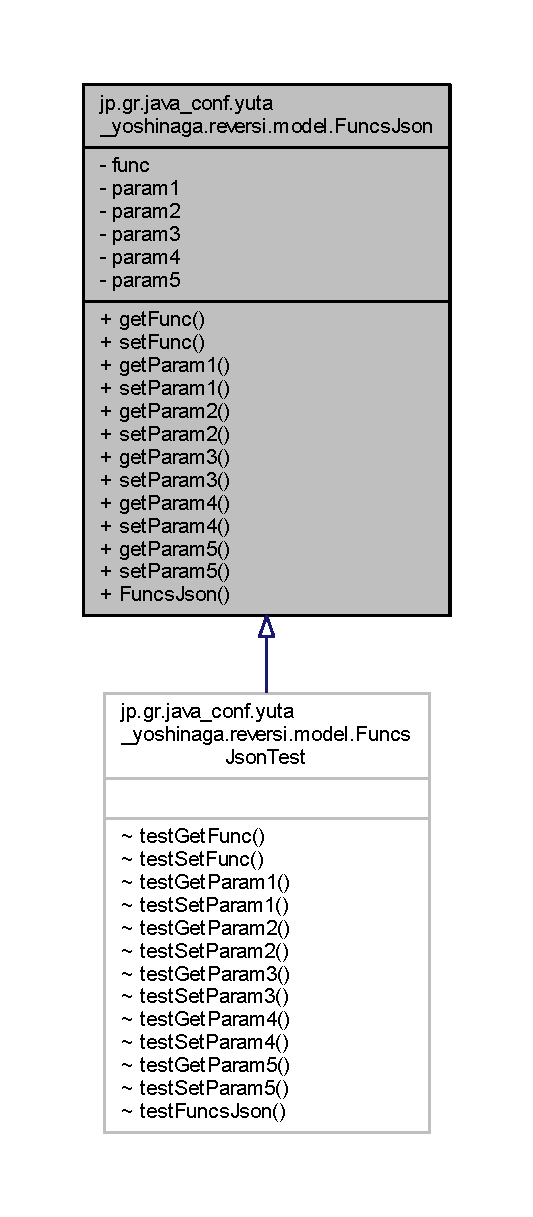
\includegraphics[height=550pt]{classjp_1_1gr_1_1java__conf_1_1yuta__yoshinaga_1_1reversi_1_1model_1_1_funcs_json__inherit__graph}
\end{center}
\end{figure}


Collaboration diagram for jp.\+gr.\+java\+\_\+conf.\+yuta\+\_\+yoshinaga.\+reversi.\+model.\+Funcs\+Json\+:
\nopagebreak
\begin{figure}[H]
\begin{center}
\leavevmode
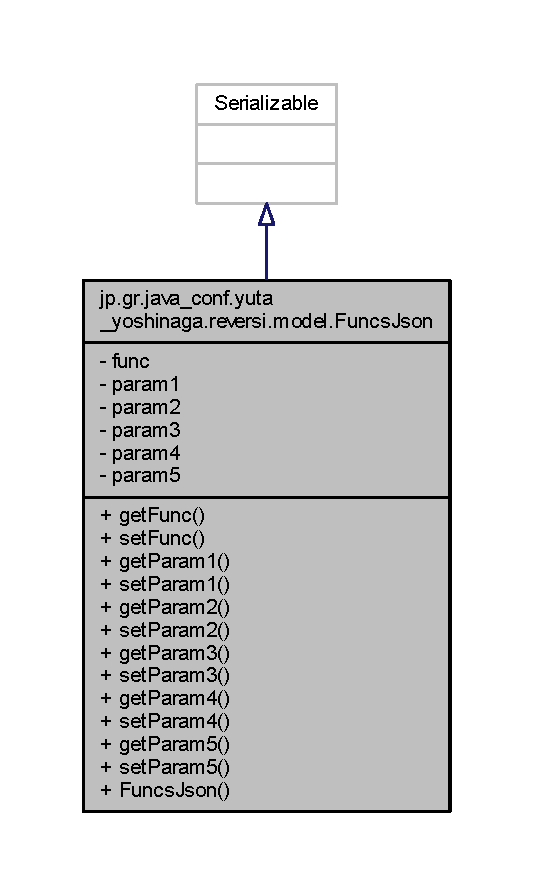
\includegraphics[width=256pt]{classjp_1_1gr_1_1java__conf_1_1yuta__yoshinaga_1_1reversi_1_1model_1_1_funcs_json__coll__graph}
\end{center}
\end{figure}
\subsection*{Public Member Functions}
\begin{DoxyCompactItemize}
\item 
String \hyperlink{classjp_1_1gr_1_1java__conf_1_1yuta__yoshinaga_1_1reversi_1_1model_1_1_funcs_json_adb9267487ecb01372d9332bee84f6378}{get\+Func} ()
\begin{DoxyCompactList}\small\item\em ゲッター \end{DoxyCompactList}\item 
void \hyperlink{classjp_1_1gr_1_1java__conf_1_1yuta__yoshinaga_1_1reversi_1_1model_1_1_funcs_json_adf43551693f93f2db4751a6fa8695d94}{set\+Func} (String \hyperlink{classjp_1_1gr_1_1java__conf_1_1yuta__yoshinaga_1_1reversi_1_1model_1_1_funcs_json_a8ca78c0a7064d28493ff6191e83f0d9b}{func})
\begin{DoxyCompactList}\small\item\em セッター \end{DoxyCompactList}\item 
String \hyperlink{classjp_1_1gr_1_1java__conf_1_1yuta__yoshinaga_1_1reversi_1_1model_1_1_funcs_json_a17ed3cd16403a8b83b61fa069556c68e}{get\+Param1} ()
\begin{DoxyCompactList}\small\item\em ゲッター \end{DoxyCompactList}\item 
void \hyperlink{classjp_1_1gr_1_1java__conf_1_1yuta__yoshinaga_1_1reversi_1_1model_1_1_funcs_json_ac7e00df5981b30ec420ef250477d9b23}{set\+Param1} (String \hyperlink{classjp_1_1gr_1_1java__conf_1_1yuta__yoshinaga_1_1reversi_1_1model_1_1_funcs_json_a2d271ee18dc5c39d0f3ab52bfde0bc27}{param1})
\begin{DoxyCompactList}\small\item\em セッター \end{DoxyCompactList}\item 
String \hyperlink{classjp_1_1gr_1_1java__conf_1_1yuta__yoshinaga_1_1reversi_1_1model_1_1_funcs_json_a032d83a0530a2f08fdaeba14eb5c1dcd}{get\+Param2} ()
\begin{DoxyCompactList}\small\item\em ゲッター \end{DoxyCompactList}\item 
void \hyperlink{classjp_1_1gr_1_1java__conf_1_1yuta__yoshinaga_1_1reversi_1_1model_1_1_funcs_json_aa1d17801d47f0d701f6792fa5f06e435}{set\+Param2} (String \hyperlink{classjp_1_1gr_1_1java__conf_1_1yuta__yoshinaga_1_1reversi_1_1model_1_1_funcs_json_a9f1f2c60a1435b78e440030fd0b5f825}{param2})
\begin{DoxyCompactList}\small\item\em セッター \end{DoxyCompactList}\item 
String \hyperlink{classjp_1_1gr_1_1java__conf_1_1yuta__yoshinaga_1_1reversi_1_1model_1_1_funcs_json_a783b331566c019ac50dd8937946d70f7}{get\+Param3} ()
\begin{DoxyCompactList}\small\item\em ゲッター \end{DoxyCompactList}\item 
void \hyperlink{classjp_1_1gr_1_1java__conf_1_1yuta__yoshinaga_1_1reversi_1_1model_1_1_funcs_json_a27bc732004c573269cb63e71c1d1abcc}{set\+Param3} (String \hyperlink{classjp_1_1gr_1_1java__conf_1_1yuta__yoshinaga_1_1reversi_1_1model_1_1_funcs_json_a90c439852b243b45c68efe96ca46fa97}{param3})
\begin{DoxyCompactList}\small\item\em セッター \end{DoxyCompactList}\item 
String \hyperlink{classjp_1_1gr_1_1java__conf_1_1yuta__yoshinaga_1_1reversi_1_1model_1_1_funcs_json_ae5c17deee7b34a5e3ed92555531bf34f}{get\+Param4} ()
\begin{DoxyCompactList}\small\item\em ゲッター \end{DoxyCompactList}\item 
void \hyperlink{classjp_1_1gr_1_1java__conf_1_1yuta__yoshinaga_1_1reversi_1_1model_1_1_funcs_json_a44af51970635551127a296e3c07db7ec}{set\+Param4} (String \hyperlink{classjp_1_1gr_1_1java__conf_1_1yuta__yoshinaga_1_1reversi_1_1model_1_1_funcs_json_a9656484f8db51bdace618bcdbc3497b9}{param4})
\begin{DoxyCompactList}\small\item\em セッター \end{DoxyCompactList}\item 
String \hyperlink{classjp_1_1gr_1_1java__conf_1_1yuta__yoshinaga_1_1reversi_1_1model_1_1_funcs_json_a86e96a579cc5f23f2842565cab755cbf}{get\+Param5} ()
\begin{DoxyCompactList}\small\item\em ゲッター \end{DoxyCompactList}\item 
void \hyperlink{classjp_1_1gr_1_1java__conf_1_1yuta__yoshinaga_1_1reversi_1_1model_1_1_funcs_json_a020f9dc27e5d795a0554ee1fda117797}{set\+Param5} (String \hyperlink{classjp_1_1gr_1_1java__conf_1_1yuta__yoshinaga_1_1reversi_1_1model_1_1_funcs_json_ac1bb96b21d4b526a690a3c1a6a88d49b}{param5})
\begin{DoxyCompactList}\small\item\em セッター \end{DoxyCompactList}\item 
\hyperlink{classjp_1_1gr_1_1java__conf_1_1yuta__yoshinaga_1_1reversi_1_1model_1_1_funcs_json_a20600564e1bb9ece956e36608a089536}{Funcs\+Json} ()
\begin{DoxyCompactList}\small\item\em コンストラクタ \end{DoxyCompactList}\end{DoxyCompactItemize}
\subsection*{Private Attributes}
\begin{DoxyCompactItemize}
\item 
\mbox{\Hypertarget{classjp_1_1gr_1_1java__conf_1_1yuta__yoshinaga_1_1reversi_1_1model_1_1_funcs_json_a8ca78c0a7064d28493ff6191e83f0d9b}\label{classjp_1_1gr_1_1java__conf_1_1yuta__yoshinaga_1_1reversi_1_1model_1_1_funcs_json_a8ca78c0a7064d28493ff6191e83f0d9b}} 
String \hyperlink{classjp_1_1gr_1_1java__conf_1_1yuta__yoshinaga_1_1reversi_1_1model_1_1_funcs_json_a8ca78c0a7064d28493ff6191e83f0d9b}{func}
\begin{DoxyCompactList}\small\item\em ファンクション \end{DoxyCompactList}\item 
\mbox{\Hypertarget{classjp_1_1gr_1_1java__conf_1_1yuta__yoshinaga_1_1reversi_1_1model_1_1_funcs_json_a2d271ee18dc5c39d0f3ab52bfde0bc27}\label{classjp_1_1gr_1_1java__conf_1_1yuta__yoshinaga_1_1reversi_1_1model_1_1_funcs_json_a2d271ee18dc5c39d0f3ab52bfde0bc27}} 
String \hyperlink{classjp_1_1gr_1_1java__conf_1_1yuta__yoshinaga_1_1reversi_1_1model_1_1_funcs_json_a2d271ee18dc5c39d0f3ab52bfde0bc27}{param1}
\begin{DoxyCompactList}\small\item\em パラメーター1 \end{DoxyCompactList}\item 
\mbox{\Hypertarget{classjp_1_1gr_1_1java__conf_1_1yuta__yoshinaga_1_1reversi_1_1model_1_1_funcs_json_a9f1f2c60a1435b78e440030fd0b5f825}\label{classjp_1_1gr_1_1java__conf_1_1yuta__yoshinaga_1_1reversi_1_1model_1_1_funcs_json_a9f1f2c60a1435b78e440030fd0b5f825}} 
String \hyperlink{classjp_1_1gr_1_1java__conf_1_1yuta__yoshinaga_1_1reversi_1_1model_1_1_funcs_json_a9f1f2c60a1435b78e440030fd0b5f825}{param2}
\begin{DoxyCompactList}\small\item\em パラメーター2 \end{DoxyCompactList}\item 
\mbox{\Hypertarget{classjp_1_1gr_1_1java__conf_1_1yuta__yoshinaga_1_1reversi_1_1model_1_1_funcs_json_a90c439852b243b45c68efe96ca46fa97}\label{classjp_1_1gr_1_1java__conf_1_1yuta__yoshinaga_1_1reversi_1_1model_1_1_funcs_json_a90c439852b243b45c68efe96ca46fa97}} 
String \hyperlink{classjp_1_1gr_1_1java__conf_1_1yuta__yoshinaga_1_1reversi_1_1model_1_1_funcs_json_a90c439852b243b45c68efe96ca46fa97}{param3}
\begin{DoxyCompactList}\small\item\em パラメーター3 \end{DoxyCompactList}\item 
\mbox{\Hypertarget{classjp_1_1gr_1_1java__conf_1_1yuta__yoshinaga_1_1reversi_1_1model_1_1_funcs_json_a9656484f8db51bdace618bcdbc3497b9}\label{classjp_1_1gr_1_1java__conf_1_1yuta__yoshinaga_1_1reversi_1_1model_1_1_funcs_json_a9656484f8db51bdace618bcdbc3497b9}} 
String \hyperlink{classjp_1_1gr_1_1java__conf_1_1yuta__yoshinaga_1_1reversi_1_1model_1_1_funcs_json_a9656484f8db51bdace618bcdbc3497b9}{param4}
\begin{DoxyCompactList}\small\item\em パラメーター4 \end{DoxyCompactList}\item 
\mbox{\Hypertarget{classjp_1_1gr_1_1java__conf_1_1yuta__yoshinaga_1_1reversi_1_1model_1_1_funcs_json_ac1bb96b21d4b526a690a3c1a6a88d49b}\label{classjp_1_1gr_1_1java__conf_1_1yuta__yoshinaga_1_1reversi_1_1model_1_1_funcs_json_ac1bb96b21d4b526a690a3c1a6a88d49b}} 
String \hyperlink{classjp_1_1gr_1_1java__conf_1_1yuta__yoshinaga_1_1reversi_1_1model_1_1_funcs_json_ac1bb96b21d4b526a690a3c1a6a88d49b}{param5}
\begin{DoxyCompactList}\small\item\em パラメーター5 \end{DoxyCompactList}\end{DoxyCompactItemize}


\subsection{Detailed Description}
ファンクション\+J\+S\+O\+Nクラス 

Definition at line 27 of file Funcs\+Json.\+java.



\subsection{Constructor \& Destructor Documentation}
\mbox{\Hypertarget{classjp_1_1gr_1_1java__conf_1_1yuta__yoshinaga_1_1reversi_1_1model_1_1_funcs_json_a20600564e1bb9ece956e36608a089536}\label{classjp_1_1gr_1_1java__conf_1_1yuta__yoshinaga_1_1reversi_1_1model_1_1_funcs_json_a20600564e1bb9ece956e36608a089536}} 
\index{jp\+::gr\+::java\+\_\+conf\+::yuta\+\_\+yoshinaga\+::reversi\+::model\+::\+Funcs\+Json@{jp\+::gr\+::java\+\_\+conf\+::yuta\+\_\+yoshinaga\+::reversi\+::model\+::\+Funcs\+Json}!Funcs\+Json@{Funcs\+Json}}
\index{Funcs\+Json@{Funcs\+Json}!jp\+::gr\+::java\+\_\+conf\+::yuta\+\_\+yoshinaga\+::reversi\+::model\+::\+Funcs\+Json@{jp\+::gr\+::java\+\_\+conf\+::yuta\+\_\+yoshinaga\+::reversi\+::model\+::\+Funcs\+Json}}
\subsubsection{\texorpdfstring{Funcs\+Json()}{FuncsJson()}}
{\footnotesize\ttfamily public jp.\+gr.\+java\+\_\+conf.\+yuta\+\_\+yoshinaga.\+reversi.\+model.\+Funcs\+Json.\+Funcs\+Json (\begin{DoxyParamCaption}{ }\end{DoxyParamCaption})}



コンストラクタ 

\begin{DoxyReturn}{Returns}
ありません 
\end{DoxyReturn}
\begin{DoxyAuthor}{Author}
Yuta Yoshinaga 
\end{DoxyAuthor}
\begin{DoxyDate}{Date}
2018.\+04.\+01 
\end{DoxyDate}


Definition at line 194 of file Funcs\+Json.\+java.



\subsection{Member Function Documentation}
\mbox{\Hypertarget{classjp_1_1gr_1_1java__conf_1_1yuta__yoshinaga_1_1reversi_1_1model_1_1_funcs_json_adb9267487ecb01372d9332bee84f6378}\label{classjp_1_1gr_1_1java__conf_1_1yuta__yoshinaga_1_1reversi_1_1model_1_1_funcs_json_adb9267487ecb01372d9332bee84f6378}} 
\index{jp\+::gr\+::java\+\_\+conf\+::yuta\+\_\+yoshinaga\+::reversi\+::model\+::\+Funcs\+Json@{jp\+::gr\+::java\+\_\+conf\+::yuta\+\_\+yoshinaga\+::reversi\+::model\+::\+Funcs\+Json}!get\+Func@{get\+Func}}
\index{get\+Func@{get\+Func}!jp\+::gr\+::java\+\_\+conf\+::yuta\+\_\+yoshinaga\+::reversi\+::model\+::\+Funcs\+Json@{jp\+::gr\+::java\+\_\+conf\+::yuta\+\_\+yoshinaga\+::reversi\+::model\+::\+Funcs\+Json}}
\subsubsection{\texorpdfstring{get\+Func()}{getFunc()}}
{\footnotesize\ttfamily String jp.\+gr.\+java\+\_\+conf.\+yuta\+\_\+yoshinaga.\+reversi.\+model.\+Funcs\+Json.\+get\+Func (\begin{DoxyParamCaption}{ }\end{DoxyParamCaption})}



ゲッター 

\begin{DoxyReturn}{Returns}
String func 
\end{DoxyReturn}
\begin{DoxyAuthor}{Author}
Yuta Yoshinaga 
\end{DoxyAuthor}
\begin{DoxyDate}{Date}
2018.\+04.\+01 
\end{DoxyDate}


Definition at line 44 of file Funcs\+Json.\+java.

\mbox{\Hypertarget{classjp_1_1gr_1_1java__conf_1_1yuta__yoshinaga_1_1reversi_1_1model_1_1_funcs_json_a17ed3cd16403a8b83b61fa069556c68e}\label{classjp_1_1gr_1_1java__conf_1_1yuta__yoshinaga_1_1reversi_1_1model_1_1_funcs_json_a17ed3cd16403a8b83b61fa069556c68e}} 
\index{jp\+::gr\+::java\+\_\+conf\+::yuta\+\_\+yoshinaga\+::reversi\+::model\+::\+Funcs\+Json@{jp\+::gr\+::java\+\_\+conf\+::yuta\+\_\+yoshinaga\+::reversi\+::model\+::\+Funcs\+Json}!get\+Param1@{get\+Param1}}
\index{get\+Param1@{get\+Param1}!jp\+::gr\+::java\+\_\+conf\+::yuta\+\_\+yoshinaga\+::reversi\+::model\+::\+Funcs\+Json@{jp\+::gr\+::java\+\_\+conf\+::yuta\+\_\+yoshinaga\+::reversi\+::model\+::\+Funcs\+Json}}
\subsubsection{\texorpdfstring{get\+Param1()}{getParam1()}}
{\footnotesize\ttfamily String jp.\+gr.\+java\+\_\+conf.\+yuta\+\_\+yoshinaga.\+reversi.\+model.\+Funcs\+Json.\+get\+Param1 (\begin{DoxyParamCaption}{ }\end{DoxyParamCaption})}



ゲッター 

\begin{DoxyReturn}{Returns}
String param1 
\end{DoxyReturn}
\begin{DoxyAuthor}{Author}
Yuta Yoshinaga 
\end{DoxyAuthor}
\begin{DoxyDate}{Date}
2018.\+04.\+01 
\end{DoxyDate}


Definition at line 69 of file Funcs\+Json.\+java.

\mbox{\Hypertarget{classjp_1_1gr_1_1java__conf_1_1yuta__yoshinaga_1_1reversi_1_1model_1_1_funcs_json_a032d83a0530a2f08fdaeba14eb5c1dcd}\label{classjp_1_1gr_1_1java__conf_1_1yuta__yoshinaga_1_1reversi_1_1model_1_1_funcs_json_a032d83a0530a2f08fdaeba14eb5c1dcd}} 
\index{jp\+::gr\+::java\+\_\+conf\+::yuta\+\_\+yoshinaga\+::reversi\+::model\+::\+Funcs\+Json@{jp\+::gr\+::java\+\_\+conf\+::yuta\+\_\+yoshinaga\+::reversi\+::model\+::\+Funcs\+Json}!get\+Param2@{get\+Param2}}
\index{get\+Param2@{get\+Param2}!jp\+::gr\+::java\+\_\+conf\+::yuta\+\_\+yoshinaga\+::reversi\+::model\+::\+Funcs\+Json@{jp\+::gr\+::java\+\_\+conf\+::yuta\+\_\+yoshinaga\+::reversi\+::model\+::\+Funcs\+Json}}
\subsubsection{\texorpdfstring{get\+Param2()}{getParam2()}}
{\footnotesize\ttfamily String jp.\+gr.\+java\+\_\+conf.\+yuta\+\_\+yoshinaga.\+reversi.\+model.\+Funcs\+Json.\+get\+Param2 (\begin{DoxyParamCaption}{ }\end{DoxyParamCaption})}



ゲッター 

\begin{DoxyReturn}{Returns}
String param2 
\end{DoxyReturn}
\begin{DoxyAuthor}{Author}
Yuta Yoshinaga 
\end{DoxyAuthor}
\begin{DoxyDate}{Date}
2018.\+04.\+01 
\end{DoxyDate}


Definition at line 94 of file Funcs\+Json.\+java.

\mbox{\Hypertarget{classjp_1_1gr_1_1java__conf_1_1yuta__yoshinaga_1_1reversi_1_1model_1_1_funcs_json_a783b331566c019ac50dd8937946d70f7}\label{classjp_1_1gr_1_1java__conf_1_1yuta__yoshinaga_1_1reversi_1_1model_1_1_funcs_json_a783b331566c019ac50dd8937946d70f7}} 
\index{jp\+::gr\+::java\+\_\+conf\+::yuta\+\_\+yoshinaga\+::reversi\+::model\+::\+Funcs\+Json@{jp\+::gr\+::java\+\_\+conf\+::yuta\+\_\+yoshinaga\+::reversi\+::model\+::\+Funcs\+Json}!get\+Param3@{get\+Param3}}
\index{get\+Param3@{get\+Param3}!jp\+::gr\+::java\+\_\+conf\+::yuta\+\_\+yoshinaga\+::reversi\+::model\+::\+Funcs\+Json@{jp\+::gr\+::java\+\_\+conf\+::yuta\+\_\+yoshinaga\+::reversi\+::model\+::\+Funcs\+Json}}
\subsubsection{\texorpdfstring{get\+Param3()}{getParam3()}}
{\footnotesize\ttfamily String jp.\+gr.\+java\+\_\+conf.\+yuta\+\_\+yoshinaga.\+reversi.\+model.\+Funcs\+Json.\+get\+Param3 (\begin{DoxyParamCaption}{ }\end{DoxyParamCaption})}



ゲッター 

\begin{DoxyReturn}{Returns}
String param3 
\end{DoxyReturn}
\begin{DoxyAuthor}{Author}
Yuta Yoshinaga 
\end{DoxyAuthor}
\begin{DoxyDate}{Date}
2018.\+04.\+01 
\end{DoxyDate}


Definition at line 119 of file Funcs\+Json.\+java.

\mbox{\Hypertarget{classjp_1_1gr_1_1java__conf_1_1yuta__yoshinaga_1_1reversi_1_1model_1_1_funcs_json_ae5c17deee7b34a5e3ed92555531bf34f}\label{classjp_1_1gr_1_1java__conf_1_1yuta__yoshinaga_1_1reversi_1_1model_1_1_funcs_json_ae5c17deee7b34a5e3ed92555531bf34f}} 
\index{jp\+::gr\+::java\+\_\+conf\+::yuta\+\_\+yoshinaga\+::reversi\+::model\+::\+Funcs\+Json@{jp\+::gr\+::java\+\_\+conf\+::yuta\+\_\+yoshinaga\+::reversi\+::model\+::\+Funcs\+Json}!get\+Param4@{get\+Param4}}
\index{get\+Param4@{get\+Param4}!jp\+::gr\+::java\+\_\+conf\+::yuta\+\_\+yoshinaga\+::reversi\+::model\+::\+Funcs\+Json@{jp\+::gr\+::java\+\_\+conf\+::yuta\+\_\+yoshinaga\+::reversi\+::model\+::\+Funcs\+Json}}
\subsubsection{\texorpdfstring{get\+Param4()}{getParam4()}}
{\footnotesize\ttfamily String jp.\+gr.\+java\+\_\+conf.\+yuta\+\_\+yoshinaga.\+reversi.\+model.\+Funcs\+Json.\+get\+Param4 (\begin{DoxyParamCaption}{ }\end{DoxyParamCaption})}



ゲッター 

\begin{DoxyReturn}{Returns}
String param4 
\end{DoxyReturn}
\begin{DoxyAuthor}{Author}
Yuta Yoshinaga 
\end{DoxyAuthor}
\begin{DoxyDate}{Date}
2018.\+04.\+01 
\end{DoxyDate}


Definition at line 144 of file Funcs\+Json.\+java.

\mbox{\Hypertarget{classjp_1_1gr_1_1java__conf_1_1yuta__yoshinaga_1_1reversi_1_1model_1_1_funcs_json_a86e96a579cc5f23f2842565cab755cbf}\label{classjp_1_1gr_1_1java__conf_1_1yuta__yoshinaga_1_1reversi_1_1model_1_1_funcs_json_a86e96a579cc5f23f2842565cab755cbf}} 
\index{jp\+::gr\+::java\+\_\+conf\+::yuta\+\_\+yoshinaga\+::reversi\+::model\+::\+Funcs\+Json@{jp\+::gr\+::java\+\_\+conf\+::yuta\+\_\+yoshinaga\+::reversi\+::model\+::\+Funcs\+Json}!get\+Param5@{get\+Param5}}
\index{get\+Param5@{get\+Param5}!jp\+::gr\+::java\+\_\+conf\+::yuta\+\_\+yoshinaga\+::reversi\+::model\+::\+Funcs\+Json@{jp\+::gr\+::java\+\_\+conf\+::yuta\+\_\+yoshinaga\+::reversi\+::model\+::\+Funcs\+Json}}
\subsubsection{\texorpdfstring{get\+Param5()}{getParam5()}}
{\footnotesize\ttfamily String jp.\+gr.\+java\+\_\+conf.\+yuta\+\_\+yoshinaga.\+reversi.\+model.\+Funcs\+Json.\+get\+Param5 (\begin{DoxyParamCaption}{ }\end{DoxyParamCaption})}



ゲッター 

\begin{DoxyReturn}{Returns}
String param5 
\end{DoxyReturn}
\begin{DoxyAuthor}{Author}
Yuta Yoshinaga 
\end{DoxyAuthor}
\begin{DoxyDate}{Date}
2018.\+04.\+01 
\end{DoxyDate}


Definition at line 169 of file Funcs\+Json.\+java.

\mbox{\Hypertarget{classjp_1_1gr_1_1java__conf_1_1yuta__yoshinaga_1_1reversi_1_1model_1_1_funcs_json_adf43551693f93f2db4751a6fa8695d94}\label{classjp_1_1gr_1_1java__conf_1_1yuta__yoshinaga_1_1reversi_1_1model_1_1_funcs_json_adf43551693f93f2db4751a6fa8695d94}} 
\index{jp\+::gr\+::java\+\_\+conf\+::yuta\+\_\+yoshinaga\+::reversi\+::model\+::\+Funcs\+Json@{jp\+::gr\+::java\+\_\+conf\+::yuta\+\_\+yoshinaga\+::reversi\+::model\+::\+Funcs\+Json}!set\+Func@{set\+Func}}
\index{set\+Func@{set\+Func}!jp\+::gr\+::java\+\_\+conf\+::yuta\+\_\+yoshinaga\+::reversi\+::model\+::\+Funcs\+Json@{jp\+::gr\+::java\+\_\+conf\+::yuta\+\_\+yoshinaga\+::reversi\+::model\+::\+Funcs\+Json}}
\subsubsection{\texorpdfstring{set\+Func()}{setFunc()}}
{\footnotesize\ttfamily void jp.\+gr.\+java\+\_\+conf.\+yuta\+\_\+yoshinaga.\+reversi.\+model.\+Funcs\+Json.\+set\+Func (\begin{DoxyParamCaption}\item[{String}]{func }\end{DoxyParamCaption})}



セッター 


\begin{DoxyParams}[1]{Parameters}
\mbox{\tt in}  & {\em String} & func \\
\hline
\end{DoxyParams}
\begin{DoxyReturn}{Returns}
ありません 
\end{DoxyReturn}
\begin{DoxyAuthor}{Author}
Yuta Yoshinaga 
\end{DoxyAuthor}
\begin{DoxyDate}{Date}
2018.\+04.\+01 
\end{DoxyDate}


Definition at line 57 of file Funcs\+Json.\+java.



Referenced by jp.\+gr.\+java\+\_\+conf.\+yuta\+\_\+yoshinaga.\+reversi.\+controller.\+Front\+Controller.\+Cur\+Col\+Msg(), jp.\+gr.\+java\+\_\+conf.\+yuta\+\_\+yoshinaga.\+reversi.\+controller.\+Front\+Controller.\+Cur\+Sts\+Msg(), jp.\+gr.\+java\+\_\+conf.\+yuta\+\_\+yoshinaga.\+reversi.\+controller.\+Front\+Controller.\+Draw\+Single(), jp.\+gr.\+java\+\_\+conf.\+yuta\+\_\+yoshinaga.\+reversi.\+controller.\+Front\+Controller.\+View\+Msg\+Dlg(), and jp.\+gr.\+java\+\_\+conf.\+yuta\+\_\+yoshinaga.\+reversi.\+controller.\+Front\+Controller.\+Wait().

Here is the caller graph for this function\+:
\nopagebreak
\begin{figure}[H]
\begin{center}
\leavevmode
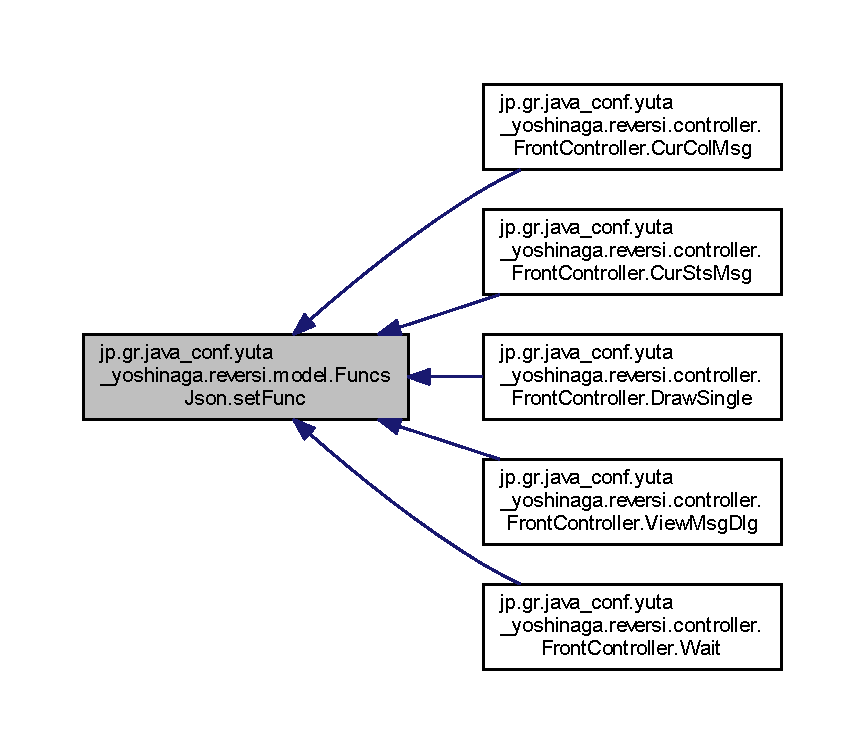
\includegraphics[width=350pt]{classjp_1_1gr_1_1java__conf_1_1yuta__yoshinaga_1_1reversi_1_1model_1_1_funcs_json_adf43551693f93f2db4751a6fa8695d94_icgraph}
\end{center}
\end{figure}
\mbox{\Hypertarget{classjp_1_1gr_1_1java__conf_1_1yuta__yoshinaga_1_1reversi_1_1model_1_1_funcs_json_ac7e00df5981b30ec420ef250477d9b23}\label{classjp_1_1gr_1_1java__conf_1_1yuta__yoshinaga_1_1reversi_1_1model_1_1_funcs_json_ac7e00df5981b30ec420ef250477d9b23}} 
\index{jp\+::gr\+::java\+\_\+conf\+::yuta\+\_\+yoshinaga\+::reversi\+::model\+::\+Funcs\+Json@{jp\+::gr\+::java\+\_\+conf\+::yuta\+\_\+yoshinaga\+::reversi\+::model\+::\+Funcs\+Json}!set\+Param1@{set\+Param1}}
\index{set\+Param1@{set\+Param1}!jp\+::gr\+::java\+\_\+conf\+::yuta\+\_\+yoshinaga\+::reversi\+::model\+::\+Funcs\+Json@{jp\+::gr\+::java\+\_\+conf\+::yuta\+\_\+yoshinaga\+::reversi\+::model\+::\+Funcs\+Json}}
\subsubsection{\texorpdfstring{set\+Param1()}{setParam1()}}
{\footnotesize\ttfamily void jp.\+gr.\+java\+\_\+conf.\+yuta\+\_\+yoshinaga.\+reversi.\+model.\+Funcs\+Json.\+set\+Param1 (\begin{DoxyParamCaption}\item[{String}]{param1 }\end{DoxyParamCaption})}



セッター 


\begin{DoxyParams}[1]{Parameters}
\mbox{\tt in}  & {\em String} & param1 \\
\hline
\end{DoxyParams}
\begin{DoxyReturn}{Returns}
ありません 
\end{DoxyReturn}
\begin{DoxyAuthor}{Author}
Yuta Yoshinaga 
\end{DoxyAuthor}
\begin{DoxyDate}{Date}
2018.\+04.\+01 
\end{DoxyDate}


Definition at line 82 of file Funcs\+Json.\+java.



Referenced by jp.\+gr.\+java\+\_\+conf.\+yuta\+\_\+yoshinaga.\+reversi.\+controller.\+Front\+Controller.\+Cur\+Col\+Msg(), jp.\+gr.\+java\+\_\+conf.\+yuta\+\_\+yoshinaga.\+reversi.\+controller.\+Front\+Controller.\+Cur\+Sts\+Msg(), jp.\+gr.\+java\+\_\+conf.\+yuta\+\_\+yoshinaga.\+reversi.\+controller.\+Front\+Controller.\+Draw\+Single(), jp.\+gr.\+java\+\_\+conf.\+yuta\+\_\+yoshinaga.\+reversi.\+controller.\+Front\+Controller.\+View\+Msg\+Dlg(), and jp.\+gr.\+java\+\_\+conf.\+yuta\+\_\+yoshinaga.\+reversi.\+controller.\+Front\+Controller.\+Wait().

Here is the caller graph for this function\+:
\nopagebreak
\begin{figure}[H]
\begin{center}
\leavevmode
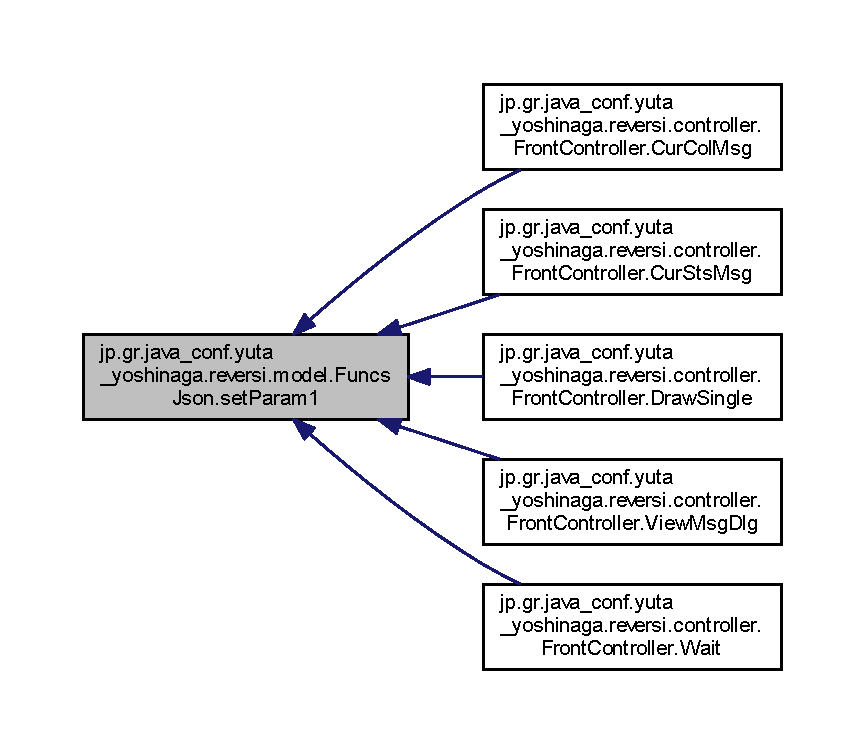
\includegraphics[width=350pt]{classjp_1_1gr_1_1java__conf_1_1yuta__yoshinaga_1_1reversi_1_1model_1_1_funcs_json_ac7e00df5981b30ec420ef250477d9b23_icgraph}
\end{center}
\end{figure}
\mbox{\Hypertarget{classjp_1_1gr_1_1java__conf_1_1yuta__yoshinaga_1_1reversi_1_1model_1_1_funcs_json_aa1d17801d47f0d701f6792fa5f06e435}\label{classjp_1_1gr_1_1java__conf_1_1yuta__yoshinaga_1_1reversi_1_1model_1_1_funcs_json_aa1d17801d47f0d701f6792fa5f06e435}} 
\index{jp\+::gr\+::java\+\_\+conf\+::yuta\+\_\+yoshinaga\+::reversi\+::model\+::\+Funcs\+Json@{jp\+::gr\+::java\+\_\+conf\+::yuta\+\_\+yoshinaga\+::reversi\+::model\+::\+Funcs\+Json}!set\+Param2@{set\+Param2}}
\index{set\+Param2@{set\+Param2}!jp\+::gr\+::java\+\_\+conf\+::yuta\+\_\+yoshinaga\+::reversi\+::model\+::\+Funcs\+Json@{jp\+::gr\+::java\+\_\+conf\+::yuta\+\_\+yoshinaga\+::reversi\+::model\+::\+Funcs\+Json}}
\subsubsection{\texorpdfstring{set\+Param2()}{setParam2()}}
{\footnotesize\ttfamily void jp.\+gr.\+java\+\_\+conf.\+yuta\+\_\+yoshinaga.\+reversi.\+model.\+Funcs\+Json.\+set\+Param2 (\begin{DoxyParamCaption}\item[{String}]{param2 }\end{DoxyParamCaption})}



セッター 


\begin{DoxyParams}[1]{Parameters}
\mbox{\tt in}  & {\em String} & param2 \\
\hline
\end{DoxyParams}
\begin{DoxyReturn}{Returns}
ありません 
\end{DoxyReturn}
\begin{DoxyAuthor}{Author}
Yuta Yoshinaga 
\end{DoxyAuthor}
\begin{DoxyDate}{Date}
2018.\+04.\+01 
\end{DoxyDate}


Definition at line 107 of file Funcs\+Json.\+java.



Referenced by jp.\+gr.\+java\+\_\+conf.\+yuta\+\_\+yoshinaga.\+reversi.\+controller.\+Front\+Controller.\+Draw\+Single(), and jp.\+gr.\+java\+\_\+conf.\+yuta\+\_\+yoshinaga.\+reversi.\+controller.\+Front\+Controller.\+View\+Msg\+Dlg().

Here is the caller graph for this function\+:
\nopagebreak
\begin{figure}[H]
\begin{center}
\leavevmode
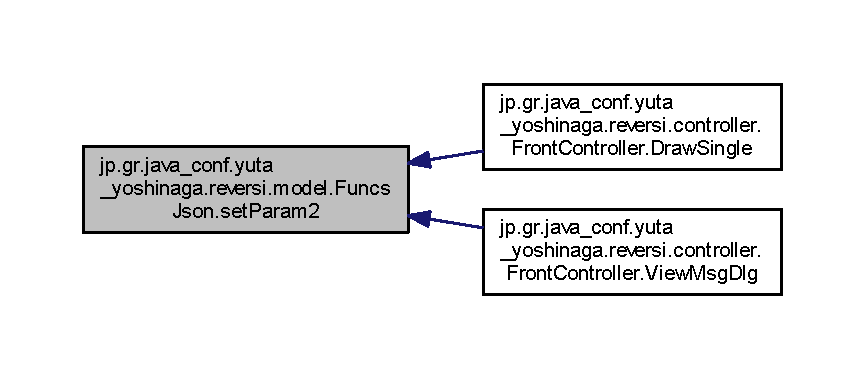
\includegraphics[width=350pt]{classjp_1_1gr_1_1java__conf_1_1yuta__yoshinaga_1_1reversi_1_1model_1_1_funcs_json_aa1d17801d47f0d701f6792fa5f06e435_icgraph}
\end{center}
\end{figure}
\mbox{\Hypertarget{classjp_1_1gr_1_1java__conf_1_1yuta__yoshinaga_1_1reversi_1_1model_1_1_funcs_json_a27bc732004c573269cb63e71c1d1abcc}\label{classjp_1_1gr_1_1java__conf_1_1yuta__yoshinaga_1_1reversi_1_1model_1_1_funcs_json_a27bc732004c573269cb63e71c1d1abcc}} 
\index{jp\+::gr\+::java\+\_\+conf\+::yuta\+\_\+yoshinaga\+::reversi\+::model\+::\+Funcs\+Json@{jp\+::gr\+::java\+\_\+conf\+::yuta\+\_\+yoshinaga\+::reversi\+::model\+::\+Funcs\+Json}!set\+Param3@{set\+Param3}}
\index{set\+Param3@{set\+Param3}!jp\+::gr\+::java\+\_\+conf\+::yuta\+\_\+yoshinaga\+::reversi\+::model\+::\+Funcs\+Json@{jp\+::gr\+::java\+\_\+conf\+::yuta\+\_\+yoshinaga\+::reversi\+::model\+::\+Funcs\+Json}}
\subsubsection{\texorpdfstring{set\+Param3()}{setParam3()}}
{\footnotesize\ttfamily void jp.\+gr.\+java\+\_\+conf.\+yuta\+\_\+yoshinaga.\+reversi.\+model.\+Funcs\+Json.\+set\+Param3 (\begin{DoxyParamCaption}\item[{String}]{param3 }\end{DoxyParamCaption})}



セッター 


\begin{DoxyParams}[1]{Parameters}
\mbox{\tt in}  & {\em String} & param3 \\
\hline
\end{DoxyParams}
\begin{DoxyReturn}{Returns}
ありません 
\end{DoxyReturn}
\begin{DoxyAuthor}{Author}
Yuta Yoshinaga 
\end{DoxyAuthor}
\begin{DoxyDate}{Date}
2018.\+04.\+01 
\end{DoxyDate}


Definition at line 132 of file Funcs\+Json.\+java.



Referenced by jp.\+gr.\+java\+\_\+conf.\+yuta\+\_\+yoshinaga.\+reversi.\+controller.\+Front\+Controller.\+Draw\+Single().

Here is the caller graph for this function\+:
\nopagebreak
\begin{figure}[H]
\begin{center}
\leavevmode
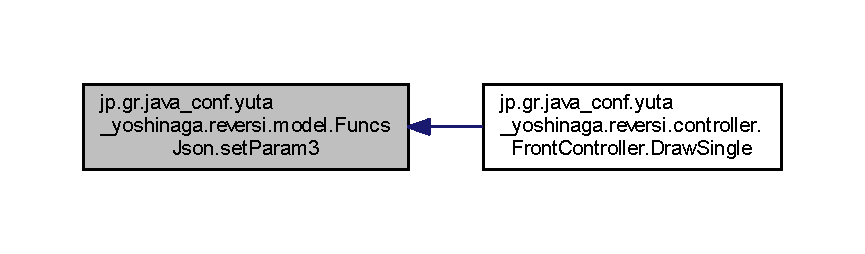
\includegraphics[width=350pt]{classjp_1_1gr_1_1java__conf_1_1yuta__yoshinaga_1_1reversi_1_1model_1_1_funcs_json_a27bc732004c573269cb63e71c1d1abcc_icgraph}
\end{center}
\end{figure}
\mbox{\Hypertarget{classjp_1_1gr_1_1java__conf_1_1yuta__yoshinaga_1_1reversi_1_1model_1_1_funcs_json_a44af51970635551127a296e3c07db7ec}\label{classjp_1_1gr_1_1java__conf_1_1yuta__yoshinaga_1_1reversi_1_1model_1_1_funcs_json_a44af51970635551127a296e3c07db7ec}} 
\index{jp\+::gr\+::java\+\_\+conf\+::yuta\+\_\+yoshinaga\+::reversi\+::model\+::\+Funcs\+Json@{jp\+::gr\+::java\+\_\+conf\+::yuta\+\_\+yoshinaga\+::reversi\+::model\+::\+Funcs\+Json}!set\+Param4@{set\+Param4}}
\index{set\+Param4@{set\+Param4}!jp\+::gr\+::java\+\_\+conf\+::yuta\+\_\+yoshinaga\+::reversi\+::model\+::\+Funcs\+Json@{jp\+::gr\+::java\+\_\+conf\+::yuta\+\_\+yoshinaga\+::reversi\+::model\+::\+Funcs\+Json}}
\subsubsection{\texorpdfstring{set\+Param4()}{setParam4()}}
{\footnotesize\ttfamily void jp.\+gr.\+java\+\_\+conf.\+yuta\+\_\+yoshinaga.\+reversi.\+model.\+Funcs\+Json.\+set\+Param4 (\begin{DoxyParamCaption}\item[{String}]{param4 }\end{DoxyParamCaption})}



セッター 


\begin{DoxyParams}[1]{Parameters}
\mbox{\tt in}  & {\em String} & param4 \\
\hline
\end{DoxyParams}
\begin{DoxyReturn}{Returns}
ありません 
\end{DoxyReturn}
\begin{DoxyAuthor}{Author}
Yuta Yoshinaga 
\end{DoxyAuthor}
\begin{DoxyDate}{Date}
2018.\+04.\+01 
\end{DoxyDate}


Definition at line 157 of file Funcs\+Json.\+java.



Referenced by jp.\+gr.\+java\+\_\+conf.\+yuta\+\_\+yoshinaga.\+reversi.\+controller.\+Front\+Controller.\+Draw\+Single().

Here is the caller graph for this function\+:
\nopagebreak
\begin{figure}[H]
\begin{center}
\leavevmode
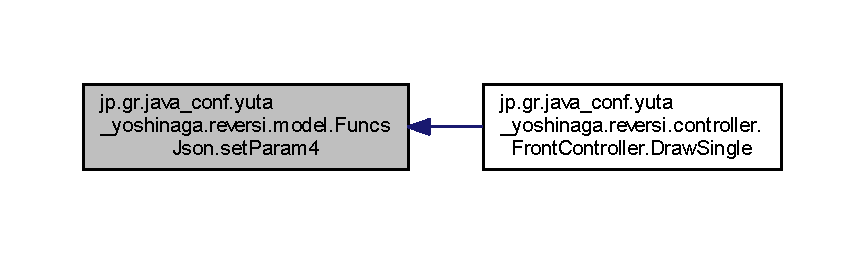
\includegraphics[width=350pt]{classjp_1_1gr_1_1java__conf_1_1yuta__yoshinaga_1_1reversi_1_1model_1_1_funcs_json_a44af51970635551127a296e3c07db7ec_icgraph}
\end{center}
\end{figure}
\mbox{\Hypertarget{classjp_1_1gr_1_1java__conf_1_1yuta__yoshinaga_1_1reversi_1_1model_1_1_funcs_json_a020f9dc27e5d795a0554ee1fda117797}\label{classjp_1_1gr_1_1java__conf_1_1yuta__yoshinaga_1_1reversi_1_1model_1_1_funcs_json_a020f9dc27e5d795a0554ee1fda117797}} 
\index{jp\+::gr\+::java\+\_\+conf\+::yuta\+\_\+yoshinaga\+::reversi\+::model\+::\+Funcs\+Json@{jp\+::gr\+::java\+\_\+conf\+::yuta\+\_\+yoshinaga\+::reversi\+::model\+::\+Funcs\+Json}!set\+Param5@{set\+Param5}}
\index{set\+Param5@{set\+Param5}!jp\+::gr\+::java\+\_\+conf\+::yuta\+\_\+yoshinaga\+::reversi\+::model\+::\+Funcs\+Json@{jp\+::gr\+::java\+\_\+conf\+::yuta\+\_\+yoshinaga\+::reversi\+::model\+::\+Funcs\+Json}}
\subsubsection{\texorpdfstring{set\+Param5()}{setParam5()}}
{\footnotesize\ttfamily void jp.\+gr.\+java\+\_\+conf.\+yuta\+\_\+yoshinaga.\+reversi.\+model.\+Funcs\+Json.\+set\+Param5 (\begin{DoxyParamCaption}\item[{String}]{param5 }\end{DoxyParamCaption})}



セッター 


\begin{DoxyParams}[1]{Parameters}
\mbox{\tt in}  & {\em String} & param5 \\
\hline
\end{DoxyParams}
\begin{DoxyReturn}{Returns}
ありません 
\end{DoxyReturn}
\begin{DoxyAuthor}{Author}
Yuta Yoshinaga 
\end{DoxyAuthor}
\begin{DoxyDate}{Date}
2018.\+04.\+01 
\end{DoxyDate}


Definition at line 182 of file Funcs\+Json.\+java.



Referenced by jp.\+gr.\+java\+\_\+conf.\+yuta\+\_\+yoshinaga.\+reversi.\+controller.\+Front\+Controller.\+Draw\+Single().

Here is the caller graph for this function\+:
\nopagebreak
\begin{figure}[H]
\begin{center}
\leavevmode
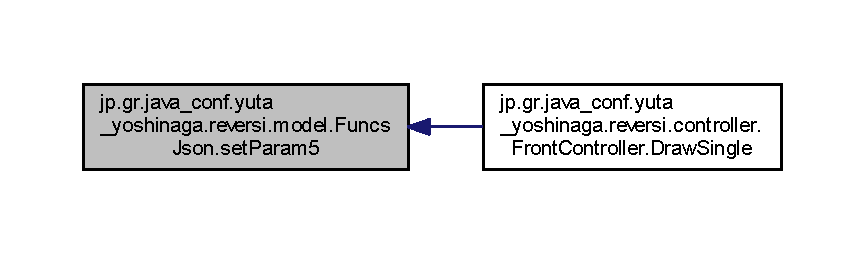
\includegraphics[width=350pt]{classjp_1_1gr_1_1java__conf_1_1yuta__yoshinaga_1_1reversi_1_1model_1_1_funcs_json_a020f9dc27e5d795a0554ee1fda117797_icgraph}
\end{center}
\end{figure}


The documentation for this class was generated from the following file\+:\begin{DoxyCompactItemize}
\item 
jp/gr/java\+\_\+conf/yuta\+\_\+yoshinaga/reversi/model/\hyperlink{_funcs_json_8java}{Funcs\+Json.\+java}\end{DoxyCompactItemize}

\hypertarget{classjp_1_1gr_1_1java__conf_1_1yuta__yoshinaga_1_1reversi_1_1model_1_1_res_json}{}\section{jp.\+gr.\+java\+\_\+conf.\+yuta\+\_\+yoshinaga.\+reversi.\+model.\+Res\+Json Class Reference}
\label{classjp_1_1gr_1_1java__conf_1_1yuta__yoshinaga_1_1reversi_1_1model_1_1_res_json}\index{jp.\+gr.\+java\+\_\+conf.\+yuta\+\_\+yoshinaga.\+reversi.\+model.\+Res\+Json@{jp.\+gr.\+java\+\_\+conf.\+yuta\+\_\+yoshinaga.\+reversi.\+model.\+Res\+Json}}


レスポンス\+J\+S\+O\+Nクラス  




Inheritance diagram for jp.\+gr.\+java\+\_\+conf.\+yuta\+\_\+yoshinaga.\+reversi.\+model.\+Res\+Json\+:\nopagebreak
\begin{figure}[H]
\begin{center}
\leavevmode
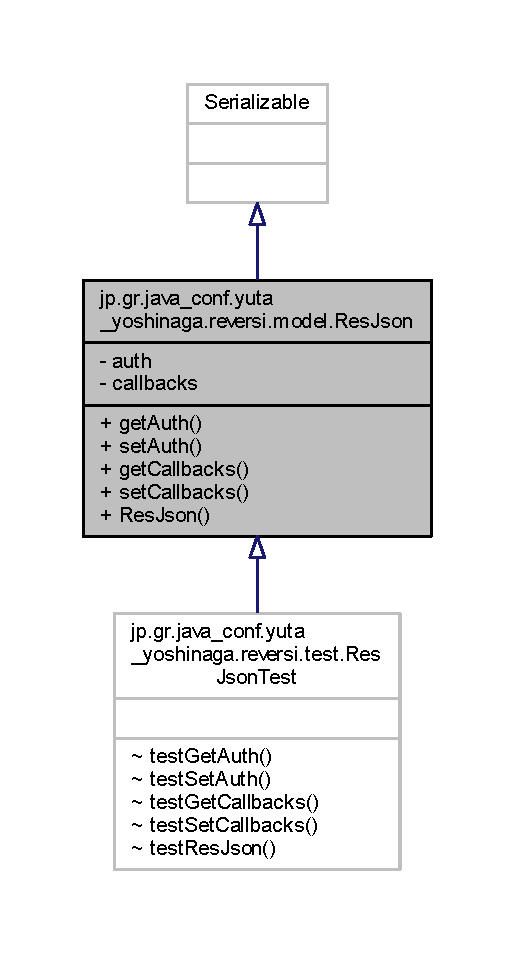
\includegraphics[width=247pt]{classjp_1_1gr_1_1java__conf_1_1yuta__yoshinaga_1_1reversi_1_1model_1_1_res_json__inherit__graph}
\end{center}
\end{figure}


Collaboration diagram for jp.\+gr.\+java\+\_\+conf.\+yuta\+\_\+yoshinaga.\+reversi.\+model.\+Res\+Json\+:\nopagebreak
\begin{figure}[H]
\begin{center}
\leavevmode
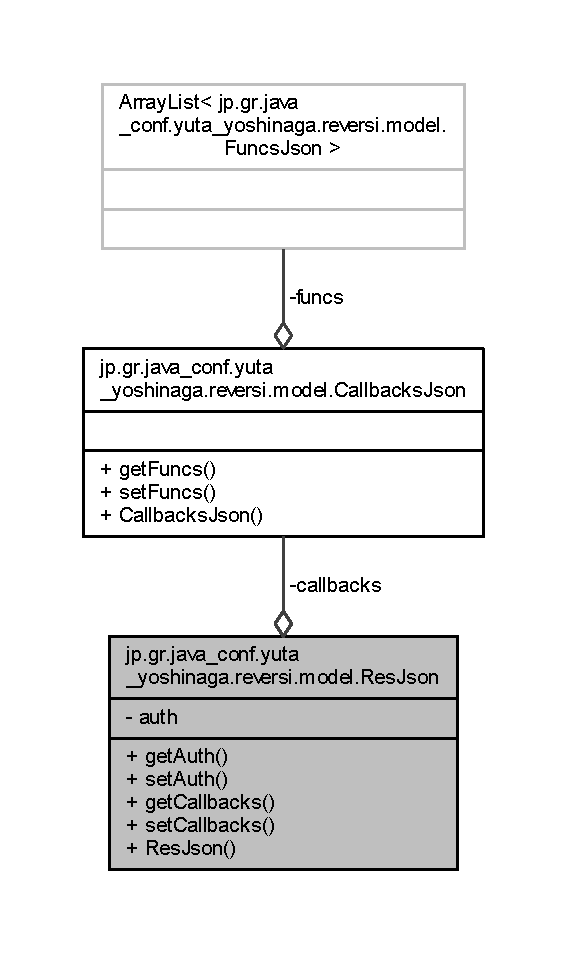
\includegraphics[width=350pt]{classjp_1_1gr_1_1java__conf_1_1yuta__yoshinaga_1_1reversi_1_1model_1_1_res_json__coll__graph}
\end{center}
\end{figure}
\subsection*{Public Member Functions}
\begin{DoxyCompactItemize}
\item 
String \mbox{\hyperlink{classjp_1_1gr_1_1java__conf_1_1yuta__yoshinaga_1_1reversi_1_1model_1_1_res_json_ae9ce58a56ca0b5302efb00692e1e78d4}{get\+Auth}} ()
\begin{DoxyCompactList}\small\item\em ゲッター \end{DoxyCompactList}\item 
void \mbox{\hyperlink{classjp_1_1gr_1_1java__conf_1_1yuta__yoshinaga_1_1reversi_1_1model_1_1_res_json_aec94a5246bf7245af19f8f72100e986c}{set\+Auth}} (String \mbox{\hyperlink{classjp_1_1gr_1_1java__conf_1_1yuta__yoshinaga_1_1reversi_1_1model_1_1_res_json_a025a6255e8c44b7a6c1e1503e1195e84}{auth}})
\begin{DoxyCompactList}\small\item\em セッター \end{DoxyCompactList}\item 
\mbox{\hyperlink{classjp_1_1gr_1_1java__conf_1_1yuta__yoshinaga_1_1reversi_1_1model_1_1_callbacks_json}{Callbacks\+Json}} \mbox{\hyperlink{classjp_1_1gr_1_1java__conf_1_1yuta__yoshinaga_1_1reversi_1_1model_1_1_res_json_a1bd6cdcfb3ea59616409b5aae1d408e2}{get\+Callbacks}} ()
\begin{DoxyCompactList}\small\item\em ゲッター \end{DoxyCompactList}\item 
void \mbox{\hyperlink{classjp_1_1gr_1_1java__conf_1_1yuta__yoshinaga_1_1reversi_1_1model_1_1_res_json_a2c93a1f6a03a04909da59238c7e68ca3}{set\+Callbacks}} (\mbox{\hyperlink{classjp_1_1gr_1_1java__conf_1_1yuta__yoshinaga_1_1reversi_1_1model_1_1_callbacks_json}{Callbacks\+Json}} \mbox{\hyperlink{classjp_1_1gr_1_1java__conf_1_1yuta__yoshinaga_1_1reversi_1_1model_1_1_res_json_a39c4406106b7bfae1aeb9c56f4a51f46}{callbacks}})
\begin{DoxyCompactList}\small\item\em セッター \end{DoxyCompactList}\item 
\mbox{\hyperlink{classjp_1_1gr_1_1java__conf_1_1yuta__yoshinaga_1_1reversi_1_1model_1_1_res_json_ac67902ff0ff40d4b25e3ded78b5098a2}{Res\+Json}} ()
\begin{DoxyCompactList}\small\item\em コンストラクタ \end{DoxyCompactList}\end{DoxyCompactItemize}
\subsection*{Private Attributes}
\begin{DoxyCompactItemize}
\item 
\mbox{\Hypertarget{classjp_1_1gr_1_1java__conf_1_1yuta__yoshinaga_1_1reversi_1_1model_1_1_res_json_a025a6255e8c44b7a6c1e1503e1195e84}\label{classjp_1_1gr_1_1java__conf_1_1yuta__yoshinaga_1_1reversi_1_1model_1_1_res_json_a025a6255e8c44b7a6c1e1503e1195e84}} 
String \mbox{\hyperlink{classjp_1_1gr_1_1java__conf_1_1yuta__yoshinaga_1_1reversi_1_1model_1_1_res_json_a025a6255e8c44b7a6c1e1503e1195e84}{auth}}
\begin{DoxyCompactList}\small\item\em リターン値 \end{DoxyCompactList}\item 
\mbox{\Hypertarget{classjp_1_1gr_1_1java__conf_1_1yuta__yoshinaga_1_1reversi_1_1model_1_1_res_json_a39c4406106b7bfae1aeb9c56f4a51f46}\label{classjp_1_1gr_1_1java__conf_1_1yuta__yoshinaga_1_1reversi_1_1model_1_1_res_json_a39c4406106b7bfae1aeb9c56f4a51f46}} 
\mbox{\hyperlink{classjp_1_1gr_1_1java__conf_1_1yuta__yoshinaga_1_1reversi_1_1model_1_1_callbacks_json}{Callbacks\+Json}} \mbox{\hyperlink{classjp_1_1gr_1_1java__conf_1_1yuta__yoshinaga_1_1reversi_1_1model_1_1_res_json_a39c4406106b7bfae1aeb9c56f4a51f46}{callbacks}}
\begin{DoxyCompactList}\small\item\em コールバックス \end{DoxyCompactList}\end{DoxyCompactItemize}


\subsection{Detailed Description}
レスポンス\+J\+S\+O\+Nクラス 

Definition at line 27 of file Res\+Json.\+java.



\subsection{Constructor \& Destructor Documentation}
\mbox{\Hypertarget{classjp_1_1gr_1_1java__conf_1_1yuta__yoshinaga_1_1reversi_1_1model_1_1_res_json_ac67902ff0ff40d4b25e3ded78b5098a2}\label{classjp_1_1gr_1_1java__conf_1_1yuta__yoshinaga_1_1reversi_1_1model_1_1_res_json_ac67902ff0ff40d4b25e3ded78b5098a2}} 
\index{jp\+::gr\+::java\+\_\+conf\+::yuta\+\_\+yoshinaga\+::reversi\+::model\+::\+Res\+Json@{jp\+::gr\+::java\+\_\+conf\+::yuta\+\_\+yoshinaga\+::reversi\+::model\+::\+Res\+Json}!Res\+Json@{Res\+Json}}
\index{Res\+Json@{Res\+Json}!jp\+::gr\+::java\+\_\+conf\+::yuta\+\_\+yoshinaga\+::reversi\+::model\+::\+Res\+Json@{jp\+::gr\+::java\+\_\+conf\+::yuta\+\_\+yoshinaga\+::reversi\+::model\+::\+Res\+Json}}
\subsubsection{\texorpdfstring{Res\+Json()}{ResJson()}}
{\footnotesize\ttfamily public jp.\+gr.\+java\+\_\+conf.\+yuta\+\_\+yoshinaga.\+reversi.\+model.\+Res\+Json.\+Res\+Json (\begin{DoxyParamCaption}{ }\end{DoxyParamCaption})}



コンストラクタ 

\begin{DoxyReturn}{Returns}
ありません 
\end{DoxyReturn}
\begin{DoxyAuthor}{Author}
Yuta Yoshinaga 
\end{DoxyAuthor}
\begin{DoxyDate}{Date}
2018.\+04.\+01 
\end{DoxyDate}


Definition at line 90 of file Res\+Json.\+java.



\subsection{Member Function Documentation}
\mbox{\Hypertarget{classjp_1_1gr_1_1java__conf_1_1yuta__yoshinaga_1_1reversi_1_1model_1_1_res_json_ae9ce58a56ca0b5302efb00692e1e78d4}\label{classjp_1_1gr_1_1java__conf_1_1yuta__yoshinaga_1_1reversi_1_1model_1_1_res_json_ae9ce58a56ca0b5302efb00692e1e78d4}} 
\index{jp\+::gr\+::java\+\_\+conf\+::yuta\+\_\+yoshinaga\+::reversi\+::model\+::\+Res\+Json@{jp\+::gr\+::java\+\_\+conf\+::yuta\+\_\+yoshinaga\+::reversi\+::model\+::\+Res\+Json}!get\+Auth@{get\+Auth}}
\index{get\+Auth@{get\+Auth}!jp\+::gr\+::java\+\_\+conf\+::yuta\+\_\+yoshinaga\+::reversi\+::model\+::\+Res\+Json@{jp\+::gr\+::java\+\_\+conf\+::yuta\+\_\+yoshinaga\+::reversi\+::model\+::\+Res\+Json}}
\subsubsection{\texorpdfstring{get\+Auth()}{getAuth()}}
{\footnotesize\ttfamily String jp.\+gr.\+java\+\_\+conf.\+yuta\+\_\+yoshinaga.\+reversi.\+model.\+Res\+Json.\+get\+Auth (\begin{DoxyParamCaption}{ }\end{DoxyParamCaption})}



ゲッター 

\begin{DoxyReturn}{Returns}
String auth 
\end{DoxyReturn}
\begin{DoxyAuthor}{Author}
Yuta Yoshinaga 
\end{DoxyAuthor}
\begin{DoxyDate}{Date}
2018.\+04.\+01 
\end{DoxyDate}


Definition at line 40 of file Res\+Json.\+java.

\mbox{\Hypertarget{classjp_1_1gr_1_1java__conf_1_1yuta__yoshinaga_1_1reversi_1_1model_1_1_res_json_a1bd6cdcfb3ea59616409b5aae1d408e2}\label{classjp_1_1gr_1_1java__conf_1_1yuta__yoshinaga_1_1reversi_1_1model_1_1_res_json_a1bd6cdcfb3ea59616409b5aae1d408e2}} 
\index{jp\+::gr\+::java\+\_\+conf\+::yuta\+\_\+yoshinaga\+::reversi\+::model\+::\+Res\+Json@{jp\+::gr\+::java\+\_\+conf\+::yuta\+\_\+yoshinaga\+::reversi\+::model\+::\+Res\+Json}!get\+Callbacks@{get\+Callbacks}}
\index{get\+Callbacks@{get\+Callbacks}!jp\+::gr\+::java\+\_\+conf\+::yuta\+\_\+yoshinaga\+::reversi\+::model\+::\+Res\+Json@{jp\+::gr\+::java\+\_\+conf\+::yuta\+\_\+yoshinaga\+::reversi\+::model\+::\+Res\+Json}}
\subsubsection{\texorpdfstring{get\+Callbacks()}{getCallbacks()}}
{\footnotesize\ttfamily \mbox{\hyperlink{classjp_1_1gr_1_1java__conf_1_1yuta__yoshinaga_1_1reversi_1_1model_1_1_callbacks_json}{Callbacks\+Json}} jp.\+gr.\+java\+\_\+conf.\+yuta\+\_\+yoshinaga.\+reversi.\+model.\+Res\+Json.\+get\+Callbacks (\begin{DoxyParamCaption}{ }\end{DoxyParamCaption})}



ゲッター 

\begin{DoxyReturn}{Returns}
\mbox{\hyperlink{classjp_1_1gr_1_1java__conf_1_1yuta__yoshinaga_1_1reversi_1_1model_1_1_callbacks_json}{Callbacks\+Json}} callbacks 
\end{DoxyReturn}
\begin{DoxyAuthor}{Author}
Yuta Yoshinaga 
\end{DoxyAuthor}
\begin{DoxyDate}{Date}
2018.\+04.\+01 
\end{DoxyDate}


Definition at line 65 of file Res\+Json.\+java.

\mbox{\Hypertarget{classjp_1_1gr_1_1java__conf_1_1yuta__yoshinaga_1_1reversi_1_1model_1_1_res_json_aec94a5246bf7245af19f8f72100e986c}\label{classjp_1_1gr_1_1java__conf_1_1yuta__yoshinaga_1_1reversi_1_1model_1_1_res_json_aec94a5246bf7245af19f8f72100e986c}} 
\index{jp\+::gr\+::java\+\_\+conf\+::yuta\+\_\+yoshinaga\+::reversi\+::model\+::\+Res\+Json@{jp\+::gr\+::java\+\_\+conf\+::yuta\+\_\+yoshinaga\+::reversi\+::model\+::\+Res\+Json}!set\+Auth@{set\+Auth}}
\index{set\+Auth@{set\+Auth}!jp\+::gr\+::java\+\_\+conf\+::yuta\+\_\+yoshinaga\+::reversi\+::model\+::\+Res\+Json@{jp\+::gr\+::java\+\_\+conf\+::yuta\+\_\+yoshinaga\+::reversi\+::model\+::\+Res\+Json}}
\subsubsection{\texorpdfstring{set\+Auth()}{setAuth()}}
{\footnotesize\ttfamily void jp.\+gr.\+java\+\_\+conf.\+yuta\+\_\+yoshinaga.\+reversi.\+model.\+Res\+Json.\+set\+Auth (\begin{DoxyParamCaption}\item[{String}]{auth }\end{DoxyParamCaption})}



セッター 


\begin{DoxyParams}[1]{Parameters}
\mbox{\tt in}  & {\em String} & auth \\
\hline
\end{DoxyParams}
\begin{DoxyReturn}{Returns}
ありません 
\end{DoxyReturn}
\begin{DoxyAuthor}{Author}
Yuta Yoshinaga 
\end{DoxyAuthor}
\begin{DoxyDate}{Date}
2018.\+04.\+01 
\end{DoxyDate}


Definition at line 53 of file Res\+Json.\+java.



Referenced by jp.\+gr.\+java\+\_\+conf.\+yuta\+\_\+yoshinaga.\+reversi.\+controller.\+Front\+Controller.\+do\+Post().

Here is the caller graph for this function\+:
\nopagebreak
\begin{figure}[H]
\begin{center}
\leavevmode
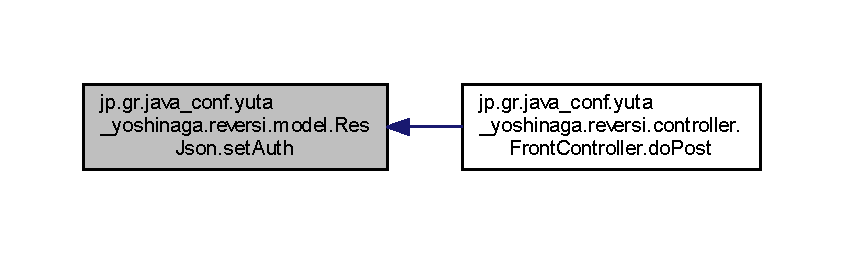
\includegraphics[width=350pt]{classjp_1_1gr_1_1java__conf_1_1yuta__yoshinaga_1_1reversi_1_1model_1_1_res_json_aec94a5246bf7245af19f8f72100e986c_icgraph}
\end{center}
\end{figure}
\mbox{\Hypertarget{classjp_1_1gr_1_1java__conf_1_1yuta__yoshinaga_1_1reversi_1_1model_1_1_res_json_a2c93a1f6a03a04909da59238c7e68ca3}\label{classjp_1_1gr_1_1java__conf_1_1yuta__yoshinaga_1_1reversi_1_1model_1_1_res_json_a2c93a1f6a03a04909da59238c7e68ca3}} 
\index{jp\+::gr\+::java\+\_\+conf\+::yuta\+\_\+yoshinaga\+::reversi\+::model\+::\+Res\+Json@{jp\+::gr\+::java\+\_\+conf\+::yuta\+\_\+yoshinaga\+::reversi\+::model\+::\+Res\+Json}!set\+Callbacks@{set\+Callbacks}}
\index{set\+Callbacks@{set\+Callbacks}!jp\+::gr\+::java\+\_\+conf\+::yuta\+\_\+yoshinaga\+::reversi\+::model\+::\+Res\+Json@{jp\+::gr\+::java\+\_\+conf\+::yuta\+\_\+yoshinaga\+::reversi\+::model\+::\+Res\+Json}}
\subsubsection{\texorpdfstring{set\+Callbacks()}{setCallbacks()}}
{\footnotesize\ttfamily void jp.\+gr.\+java\+\_\+conf.\+yuta\+\_\+yoshinaga.\+reversi.\+model.\+Res\+Json.\+set\+Callbacks (\begin{DoxyParamCaption}\item[{\mbox{\hyperlink{classjp_1_1gr_1_1java__conf_1_1yuta__yoshinaga_1_1reversi_1_1model_1_1_callbacks_json}{Callbacks\+Json}}}]{callbacks }\end{DoxyParamCaption})}



セッター 


\begin{DoxyParams}[1]{Parameters}
\mbox{\tt in}  & {\em String} & callbacks \\
\hline
\end{DoxyParams}
\begin{DoxyReturn}{Returns}
ありません 
\end{DoxyReturn}
\begin{DoxyAuthor}{Author}
Yuta Yoshinaga 
\end{DoxyAuthor}
\begin{DoxyDate}{Date}
2018.\+04.\+01 
\end{DoxyDate}


Definition at line 78 of file Res\+Json.\+java.



Referenced by jp.\+gr.\+java\+\_\+conf.\+yuta\+\_\+yoshinaga.\+reversi.\+controller.\+Front\+Controller.\+do\+Post().

Here is the caller graph for this function\+:
\nopagebreak
\begin{figure}[H]
\begin{center}
\leavevmode
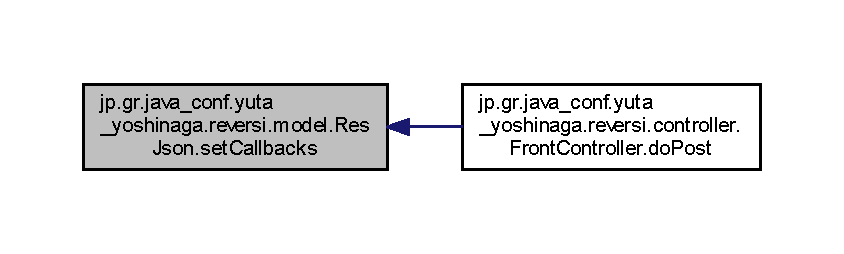
\includegraphics[width=350pt]{classjp_1_1gr_1_1java__conf_1_1yuta__yoshinaga_1_1reversi_1_1model_1_1_res_json_a2c93a1f6a03a04909da59238c7e68ca3_icgraph}
\end{center}
\end{figure}


The documentation for this class was generated from the following file\+:\begin{DoxyCompactItemize}
\item 
jp/gr/java\+\_\+conf/yuta\+\_\+yoshinaga/reversi/model/\mbox{\hyperlink{_res_json_8java}{Res\+Json.\+java}}\end{DoxyCompactItemize}

\hypertarget{classjp_1_1gr_1_1java__conf_1_1yuta__yoshinaga_1_1reversi_1_1model_1_1_reversi}{}\section{jp.\+gr.\+java\+\_\+conf.\+yuta\+\_\+yoshinaga.\+reversi.\+model.\+Reversi Class Reference}
\label{classjp_1_1gr_1_1java__conf_1_1yuta__yoshinaga_1_1reversi_1_1model_1_1_reversi}\index{jp.\+gr.\+java\+\_\+conf.\+yuta\+\_\+yoshinaga.\+reversi.\+model.\+Reversi@{jp.\+gr.\+java\+\_\+conf.\+yuta\+\_\+yoshinaga.\+reversi.\+model.\+Reversi}}


リバーシクラス  




Inheritance diagram for jp.\+gr.\+java\+\_\+conf.\+yuta\+\_\+yoshinaga.\+reversi.\+model.\+Reversi\+:\nopagebreak
\begin{figure}[H]
\begin{center}
\leavevmode
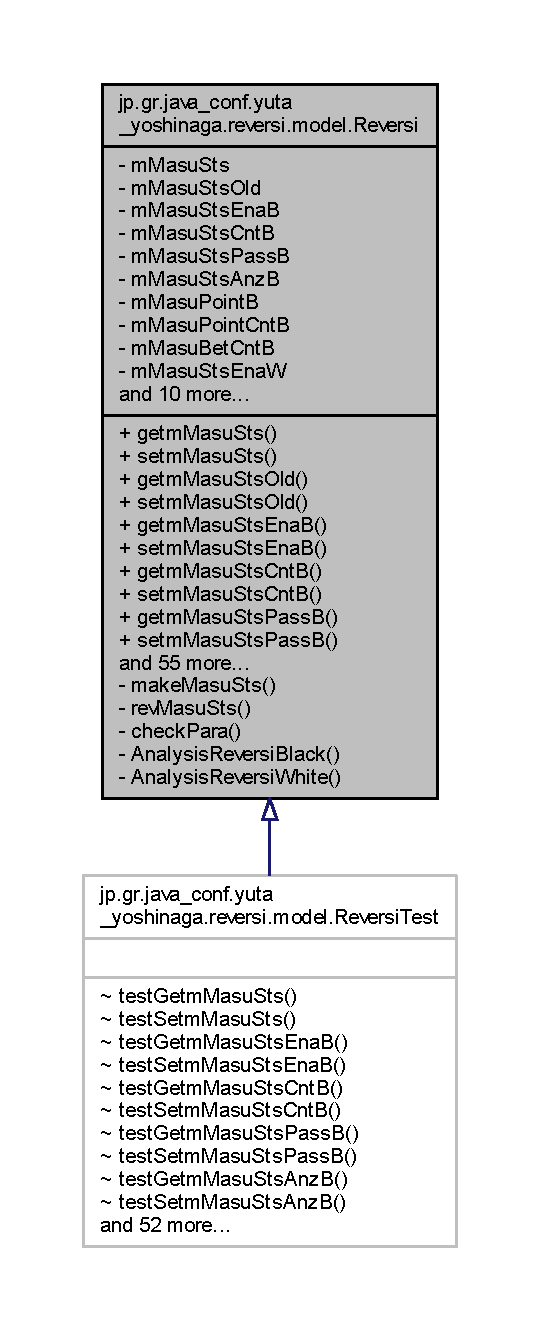
\includegraphics[height=550pt]{classjp_1_1gr_1_1java__conf_1_1yuta__yoshinaga_1_1reversi_1_1model_1_1_reversi__inherit__graph}
\end{center}
\end{figure}


Collaboration diagram for jp.\+gr.\+java\+\_\+conf.\+yuta\+\_\+yoshinaga.\+reversi.\+model.\+Reversi\+:\nopagebreak
\begin{figure}[H]
\begin{center}
\leavevmode
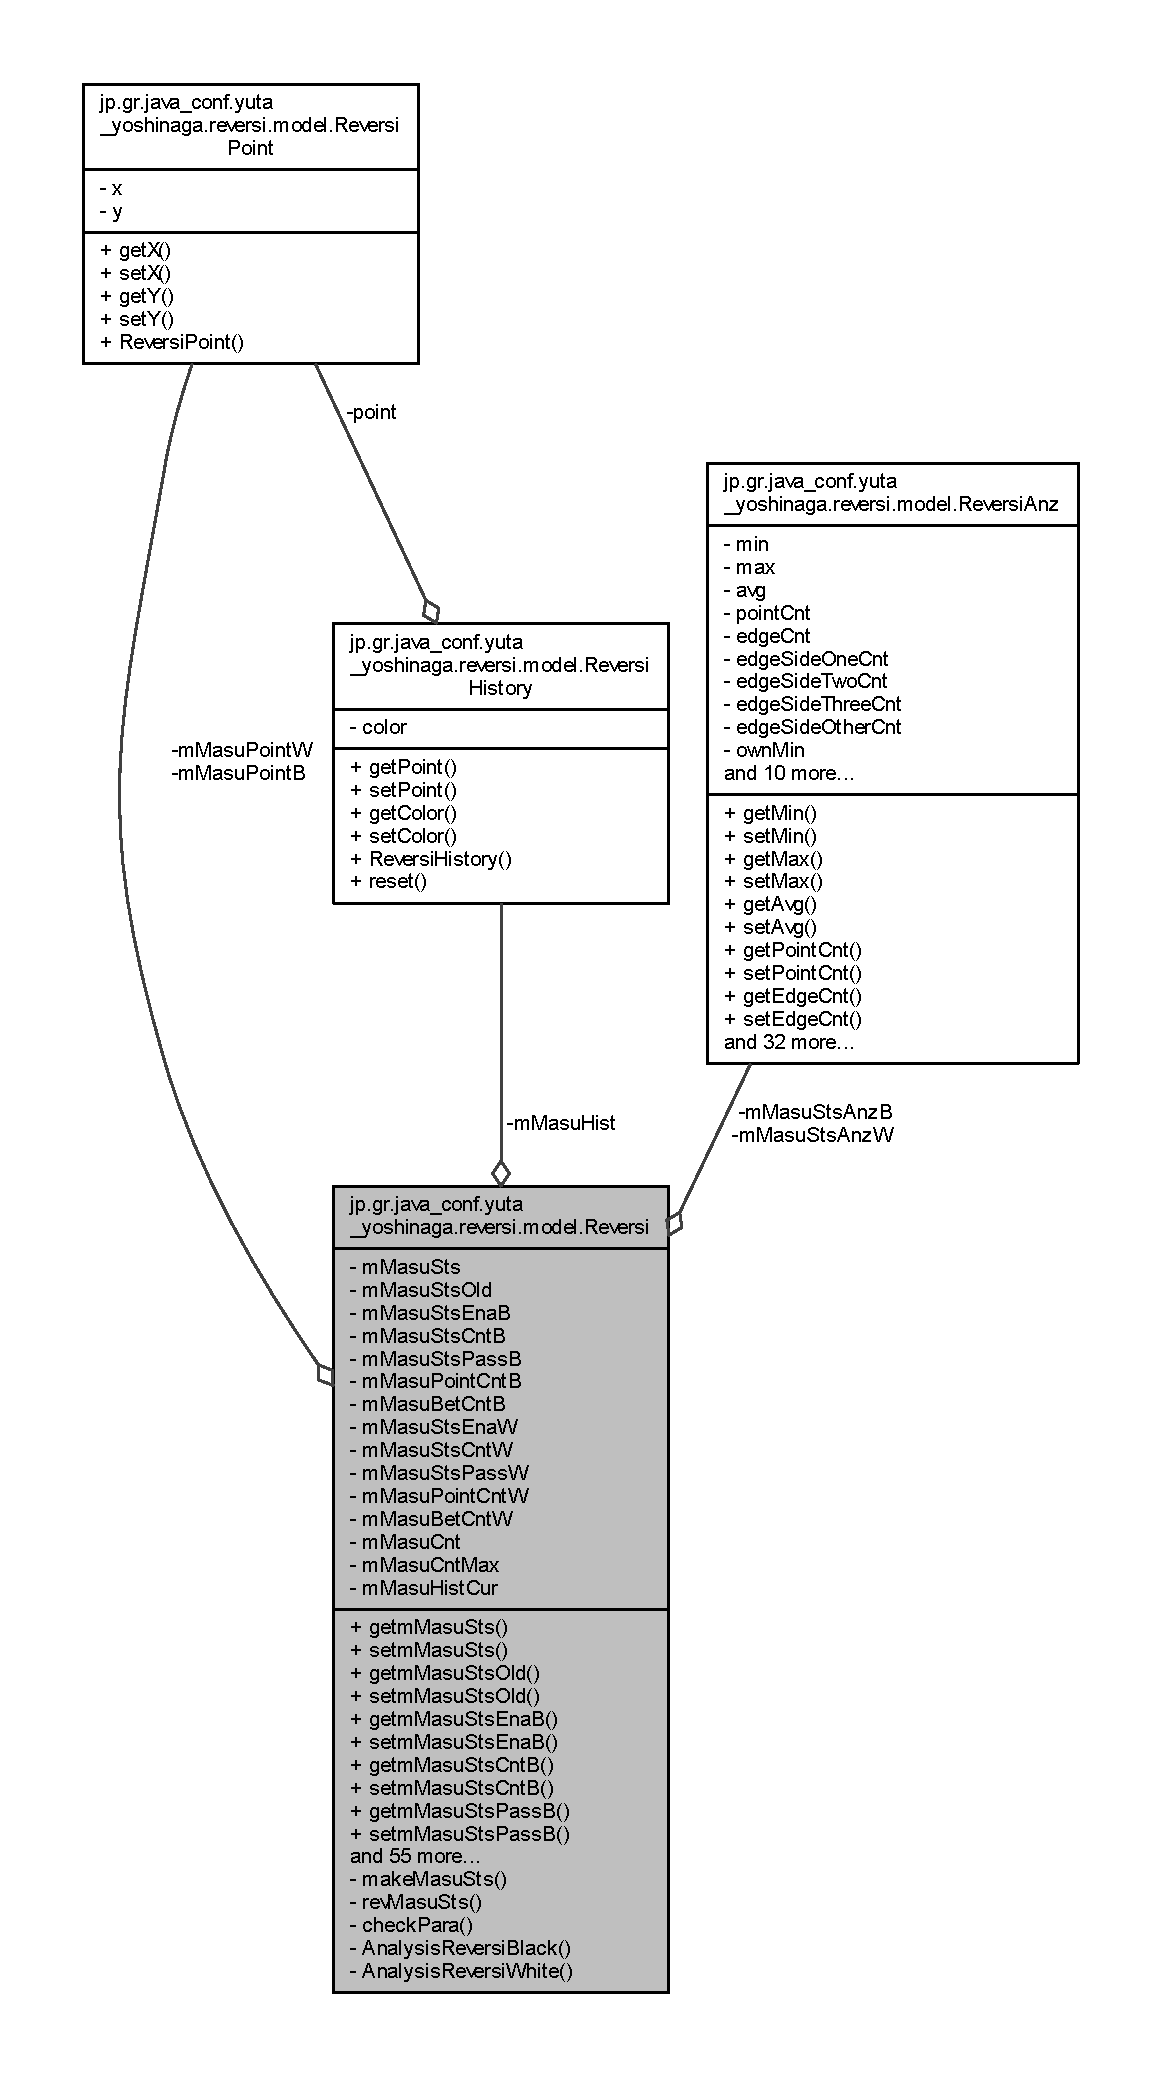
\includegraphics[height=550pt]{classjp_1_1gr_1_1java__conf_1_1yuta__yoshinaga_1_1reversi_1_1model_1_1_reversi__coll__graph}
\end{center}
\end{figure}
\subsection*{Public Member Functions}
\begin{DoxyCompactItemize}
\item 
\mbox{\Hypertarget{classjp_1_1gr_1_1java__conf_1_1yuta__yoshinaga_1_1reversi_1_1model_1_1_reversi_a21646bade723cd8683203843c5ced422}\label{classjp_1_1gr_1_1java__conf_1_1yuta__yoshinaga_1_1reversi_1_1model_1_1_reversi_a21646bade723cd8683203843c5ced422}} 
int \mbox{[}$\,$\mbox{]}\mbox{[}$\,$\mbox{]} {\bfseries getm\+Masu\+Sts} ()
\item 
void \hyperlink{classjp_1_1gr_1_1java__conf_1_1yuta__yoshinaga_1_1reversi_1_1model_1_1_reversi_a412ca568b8d8d1aeee39c22993cfcefd}{setm\+Masu\+Sts} (int\mbox{[}$\,$\mbox{]}\mbox{[}$\,$\mbox{]} \hyperlink{classjp_1_1gr_1_1java__conf_1_1yuta__yoshinaga_1_1reversi_1_1model_1_1_reversi_a8046f50bdd41778ecb7d08ac72b497d0}{m\+Masu\+Sts})
\begin{DoxyCompactList}\small\item\em セッター \end{DoxyCompactList}\item 
\mbox{\Hypertarget{classjp_1_1gr_1_1java__conf_1_1yuta__yoshinaga_1_1reversi_1_1model_1_1_reversi_a2bb0c499c3643a8b8a6a88c1167d59ea}\label{classjp_1_1gr_1_1java__conf_1_1yuta__yoshinaga_1_1reversi_1_1model_1_1_reversi_a2bb0c499c3643a8b8a6a88c1167d59ea}} 
int \mbox{[}$\,$\mbox{]}\mbox{[}$\,$\mbox{]} {\bfseries getm\+Masu\+Sts\+Old} ()
\item 
void \hyperlink{classjp_1_1gr_1_1java__conf_1_1yuta__yoshinaga_1_1reversi_1_1model_1_1_reversi_aadea9ebffe1ab20a3f0ef4d348d0dba3}{setm\+Masu\+Sts\+Old} (int\mbox{[}$\,$\mbox{]}\mbox{[}$\,$\mbox{]} \hyperlink{classjp_1_1gr_1_1java__conf_1_1yuta__yoshinaga_1_1reversi_1_1model_1_1_reversi_ac103fe1c07d3c942e4909ade4ae3a062}{m\+Masu\+Sts\+Old})
\begin{DoxyCompactList}\small\item\em セッター \end{DoxyCompactList}\item 
\mbox{\Hypertarget{classjp_1_1gr_1_1java__conf_1_1yuta__yoshinaga_1_1reversi_1_1model_1_1_reversi_ae804139f32bbfc300ca7b488d26596ca}\label{classjp_1_1gr_1_1java__conf_1_1yuta__yoshinaga_1_1reversi_1_1model_1_1_reversi_ae804139f32bbfc300ca7b488d26596ca}} 
int \mbox{[}$\,$\mbox{]}\mbox{[}$\,$\mbox{]} {\bfseries getm\+Masu\+Sts\+EnaB} ()
\item 
void \hyperlink{classjp_1_1gr_1_1java__conf_1_1yuta__yoshinaga_1_1reversi_1_1model_1_1_reversi_a7ac6d610eab47a4a785e68942abf050e}{setm\+Masu\+Sts\+EnaB} (int\mbox{[}$\,$\mbox{]}\mbox{[}$\,$\mbox{]} \hyperlink{classjp_1_1gr_1_1java__conf_1_1yuta__yoshinaga_1_1reversi_1_1model_1_1_reversi_a8ef5d1359955d380626061b8da01badf}{m\+Masu\+Sts\+EnaB})
\begin{DoxyCompactList}\small\item\em セッター \end{DoxyCompactList}\item 
\mbox{\Hypertarget{classjp_1_1gr_1_1java__conf_1_1yuta__yoshinaga_1_1reversi_1_1model_1_1_reversi_a620d4c52000eda32adccabe150fb3e8b}\label{classjp_1_1gr_1_1java__conf_1_1yuta__yoshinaga_1_1reversi_1_1model_1_1_reversi_a620d4c52000eda32adccabe150fb3e8b}} 
int \mbox{[}$\,$\mbox{]}\mbox{[}$\,$\mbox{]} {\bfseries getm\+Masu\+Sts\+CntB} ()
\item 
void \hyperlink{classjp_1_1gr_1_1java__conf_1_1yuta__yoshinaga_1_1reversi_1_1model_1_1_reversi_a9da75ee353d369b909c36d9f4ca5e967}{setm\+Masu\+Sts\+CntB} (int\mbox{[}$\,$\mbox{]}\mbox{[}$\,$\mbox{]} \hyperlink{classjp_1_1gr_1_1java__conf_1_1yuta__yoshinaga_1_1reversi_1_1model_1_1_reversi_a564e11e1ebe3ba48214d3af5505aa3a6}{m\+Masu\+Sts\+CntB})
\begin{DoxyCompactList}\small\item\em セッター \end{DoxyCompactList}\item 
\mbox{\Hypertarget{classjp_1_1gr_1_1java__conf_1_1yuta__yoshinaga_1_1reversi_1_1model_1_1_reversi_a59a22503188f4e435a14169d0af7535b}\label{classjp_1_1gr_1_1java__conf_1_1yuta__yoshinaga_1_1reversi_1_1model_1_1_reversi_a59a22503188f4e435a14169d0af7535b}} 
int \mbox{[}$\,$\mbox{]}\mbox{[}$\,$\mbox{]} {\bfseries getm\+Masu\+Sts\+PassB} ()
\item 
void \hyperlink{classjp_1_1gr_1_1java__conf_1_1yuta__yoshinaga_1_1reversi_1_1model_1_1_reversi_abe3cffd1d54da13f683504336828a4eb}{setm\+Masu\+Sts\+PassB} (int\mbox{[}$\,$\mbox{]}\mbox{[}$\,$\mbox{]} \hyperlink{classjp_1_1gr_1_1java__conf_1_1yuta__yoshinaga_1_1reversi_1_1model_1_1_reversi_ad2104bbe2d1da001acb0fae1ff31d57a}{m\+Masu\+Sts\+PassB})
\begin{DoxyCompactList}\small\item\em セッター \end{DoxyCompactList}\item 
\mbox{\Hypertarget{classjp_1_1gr_1_1java__conf_1_1yuta__yoshinaga_1_1reversi_1_1model_1_1_reversi_a1c3ba6c2580905227538f89386e38736}\label{classjp_1_1gr_1_1java__conf_1_1yuta__yoshinaga_1_1reversi_1_1model_1_1_reversi_a1c3ba6c2580905227538f89386e38736}} 
\hyperlink{classjp_1_1gr_1_1java__conf_1_1yuta__yoshinaga_1_1reversi_1_1model_1_1_reversi_anz}{Reversi\+Anz} \mbox{[}$\,$\mbox{]}\mbox{[}$\,$\mbox{]} {\bfseries getm\+Masu\+Sts\+AnzB} ()
\item 
void \hyperlink{classjp_1_1gr_1_1java__conf_1_1yuta__yoshinaga_1_1reversi_1_1model_1_1_reversi_ad955214e48b277da67f8b0aa7a91f4e0}{setm\+Masu\+Sts\+AnzB} (\hyperlink{classjp_1_1gr_1_1java__conf_1_1yuta__yoshinaga_1_1reversi_1_1model_1_1_reversi_anz}{Reversi\+Anz}\mbox{[}$\,$\mbox{]}\mbox{[}$\,$\mbox{]} \hyperlink{classjp_1_1gr_1_1java__conf_1_1yuta__yoshinaga_1_1reversi_1_1model_1_1_reversi_afd4e2cb262d61e640b098b1563956bb6}{m\+Masu\+Sts\+AnzB})
\begin{DoxyCompactList}\small\item\em セッター \end{DoxyCompactList}\item 
\mbox{\Hypertarget{classjp_1_1gr_1_1java__conf_1_1yuta__yoshinaga_1_1reversi_1_1model_1_1_reversi_afb6caed6814a12d02d7d9e2a7d7cd9ef}\label{classjp_1_1gr_1_1java__conf_1_1yuta__yoshinaga_1_1reversi_1_1model_1_1_reversi_afb6caed6814a12d02d7d9e2a7d7cd9ef}} 
\hyperlink{classjp_1_1gr_1_1java__conf_1_1yuta__yoshinaga_1_1reversi_1_1model_1_1_reversi_point}{Reversi\+Point} \mbox{[}$\,$\mbox{]} {\bfseries getm\+Masu\+PointB} ()
\item 
void \hyperlink{classjp_1_1gr_1_1java__conf_1_1yuta__yoshinaga_1_1reversi_1_1model_1_1_reversi_a84a16cc376a04c1fad8ad47a637f5363}{setm\+Masu\+PointB} (\hyperlink{classjp_1_1gr_1_1java__conf_1_1yuta__yoshinaga_1_1reversi_1_1model_1_1_reversi_point}{Reversi\+Point}\mbox{[}$\,$\mbox{]} \hyperlink{classjp_1_1gr_1_1java__conf_1_1yuta__yoshinaga_1_1reversi_1_1model_1_1_reversi_a544d45bb741e4436f2eae49d93ceb00c}{m\+Masu\+PointB})
\begin{DoxyCompactList}\small\item\em セッター \end{DoxyCompactList}\item 
int \hyperlink{classjp_1_1gr_1_1java__conf_1_1yuta__yoshinaga_1_1reversi_1_1model_1_1_reversi_ad2c4e4e56738790789c00c7ce53d1f24}{getm\+Masu\+Point\+CntB} ()
\begin{DoxyCompactList}\small\item\em ゲッター \end{DoxyCompactList}\item 
void \hyperlink{classjp_1_1gr_1_1java__conf_1_1yuta__yoshinaga_1_1reversi_1_1model_1_1_reversi_a9a80afb94b9a49bb92a0187385bf02a7}{setm\+Masu\+Point\+CntB} (int \hyperlink{classjp_1_1gr_1_1java__conf_1_1yuta__yoshinaga_1_1reversi_1_1model_1_1_reversi_ac49a25681eb3e227f42cc225803241d3}{m\+Masu\+Point\+CntB})
\begin{DoxyCompactList}\small\item\em セッター \end{DoxyCompactList}\item 
int \hyperlink{classjp_1_1gr_1_1java__conf_1_1yuta__yoshinaga_1_1reversi_1_1model_1_1_reversi_a9eca6c8f158433303079e333a29ee564}{getm\+Masu\+Bet\+CntB} ()
\begin{DoxyCompactList}\small\item\em ゲッター \end{DoxyCompactList}\item 
void \hyperlink{classjp_1_1gr_1_1java__conf_1_1yuta__yoshinaga_1_1reversi_1_1model_1_1_reversi_af198b74e838b49c40661730ac639fae5}{setm\+Masu\+Bet\+CntB} (int \hyperlink{classjp_1_1gr_1_1java__conf_1_1yuta__yoshinaga_1_1reversi_1_1model_1_1_reversi_ad09160526b0dce0e8d0606c85ce52e3f}{m\+Masu\+Bet\+CntB})
\begin{DoxyCompactList}\small\item\em セッター \end{DoxyCompactList}\item 
\mbox{\Hypertarget{classjp_1_1gr_1_1java__conf_1_1yuta__yoshinaga_1_1reversi_1_1model_1_1_reversi_a64f7bf09f1ce914bb51a7727da306307}\label{classjp_1_1gr_1_1java__conf_1_1yuta__yoshinaga_1_1reversi_1_1model_1_1_reversi_a64f7bf09f1ce914bb51a7727da306307}} 
int \mbox{[}$\,$\mbox{]}\mbox{[}$\,$\mbox{]} {\bfseries getm\+Masu\+Sts\+EnaW} ()
\item 
void \hyperlink{classjp_1_1gr_1_1java__conf_1_1yuta__yoshinaga_1_1reversi_1_1model_1_1_reversi_adf6237e04e5d6966d96e2f4c1e59bb00}{setm\+Masu\+Sts\+EnaW} (int\mbox{[}$\,$\mbox{]}\mbox{[}$\,$\mbox{]} \hyperlink{classjp_1_1gr_1_1java__conf_1_1yuta__yoshinaga_1_1reversi_1_1model_1_1_reversi_a13c5c066fa8e0f0834c583448839dbba}{m\+Masu\+Sts\+EnaW})
\begin{DoxyCompactList}\small\item\em セッター \end{DoxyCompactList}\item 
\mbox{\Hypertarget{classjp_1_1gr_1_1java__conf_1_1yuta__yoshinaga_1_1reversi_1_1model_1_1_reversi_a2512debcaa43b15d4200479e2a201bc4}\label{classjp_1_1gr_1_1java__conf_1_1yuta__yoshinaga_1_1reversi_1_1model_1_1_reversi_a2512debcaa43b15d4200479e2a201bc4}} 
int \mbox{[}$\,$\mbox{]}\mbox{[}$\,$\mbox{]} {\bfseries getm\+Masu\+Sts\+CntW} ()
\item 
void \hyperlink{classjp_1_1gr_1_1java__conf_1_1yuta__yoshinaga_1_1reversi_1_1model_1_1_reversi_a539082d7e05f2f91ac1350eae0de4f7d}{setm\+Masu\+Sts\+CntW} (int\mbox{[}$\,$\mbox{]}\mbox{[}$\,$\mbox{]} \hyperlink{classjp_1_1gr_1_1java__conf_1_1yuta__yoshinaga_1_1reversi_1_1model_1_1_reversi_af0915b3095c755c161b9b8c5221588fb}{m\+Masu\+Sts\+CntW})
\begin{DoxyCompactList}\small\item\em セッター \end{DoxyCompactList}\item 
\mbox{\Hypertarget{classjp_1_1gr_1_1java__conf_1_1yuta__yoshinaga_1_1reversi_1_1model_1_1_reversi_a68ed78d0b9622ac799d03b1a620949cb}\label{classjp_1_1gr_1_1java__conf_1_1yuta__yoshinaga_1_1reversi_1_1model_1_1_reversi_a68ed78d0b9622ac799d03b1a620949cb}} 
int \mbox{[}$\,$\mbox{]}\mbox{[}$\,$\mbox{]} {\bfseries getm\+Masu\+Sts\+PassW} ()
\item 
void \hyperlink{classjp_1_1gr_1_1java__conf_1_1yuta__yoshinaga_1_1reversi_1_1model_1_1_reversi_abc3f2428451363bde194d0655ef2ffd7}{setm\+Masu\+Sts\+PassW} (int\mbox{[}$\,$\mbox{]}\mbox{[}$\,$\mbox{]} \hyperlink{classjp_1_1gr_1_1java__conf_1_1yuta__yoshinaga_1_1reversi_1_1model_1_1_reversi_a4f8ec2166d25bd9ee669f4ce3624d403}{m\+Masu\+Sts\+PassW})
\begin{DoxyCompactList}\small\item\em セッター \end{DoxyCompactList}\item 
\mbox{\Hypertarget{classjp_1_1gr_1_1java__conf_1_1yuta__yoshinaga_1_1reversi_1_1model_1_1_reversi_ab7be991ed620905e653345ef7718bfc9}\label{classjp_1_1gr_1_1java__conf_1_1yuta__yoshinaga_1_1reversi_1_1model_1_1_reversi_ab7be991ed620905e653345ef7718bfc9}} 
\hyperlink{classjp_1_1gr_1_1java__conf_1_1yuta__yoshinaga_1_1reversi_1_1model_1_1_reversi_anz}{Reversi\+Anz} \mbox{[}$\,$\mbox{]}\mbox{[}$\,$\mbox{]} {\bfseries getm\+Masu\+Sts\+AnzW} ()
\item 
void \hyperlink{classjp_1_1gr_1_1java__conf_1_1yuta__yoshinaga_1_1reversi_1_1model_1_1_reversi_ad12845e3fae70c9d84372147267e89f9}{setm\+Masu\+Sts\+AnzW} (\hyperlink{classjp_1_1gr_1_1java__conf_1_1yuta__yoshinaga_1_1reversi_1_1model_1_1_reversi_anz}{Reversi\+Anz}\mbox{[}$\,$\mbox{]}\mbox{[}$\,$\mbox{]} \hyperlink{classjp_1_1gr_1_1java__conf_1_1yuta__yoshinaga_1_1reversi_1_1model_1_1_reversi_aa0f52d94572b3b866b464c91dc0575ff}{m\+Masu\+Sts\+AnzW})
\begin{DoxyCompactList}\small\item\em セッター \end{DoxyCompactList}\item 
\mbox{\Hypertarget{classjp_1_1gr_1_1java__conf_1_1yuta__yoshinaga_1_1reversi_1_1model_1_1_reversi_a526ca595a5a4f9dbfb9e20ddf48c9798}\label{classjp_1_1gr_1_1java__conf_1_1yuta__yoshinaga_1_1reversi_1_1model_1_1_reversi_a526ca595a5a4f9dbfb9e20ddf48c9798}} 
\hyperlink{classjp_1_1gr_1_1java__conf_1_1yuta__yoshinaga_1_1reversi_1_1model_1_1_reversi_point}{Reversi\+Point} \mbox{[}$\,$\mbox{]} {\bfseries getm\+Masu\+PointW} ()
\item 
void \hyperlink{classjp_1_1gr_1_1java__conf_1_1yuta__yoshinaga_1_1reversi_1_1model_1_1_reversi_a3c7a1dfd53c9d84e23bb7c9895657261}{setm\+Masu\+PointW} (\hyperlink{classjp_1_1gr_1_1java__conf_1_1yuta__yoshinaga_1_1reversi_1_1model_1_1_reversi_point}{Reversi\+Point}\mbox{[}$\,$\mbox{]} \hyperlink{classjp_1_1gr_1_1java__conf_1_1yuta__yoshinaga_1_1reversi_1_1model_1_1_reversi_a254c60242b0c2e4c4ffc4b211bb5794b}{m\+Masu\+PointW})
\begin{DoxyCompactList}\small\item\em セッター \end{DoxyCompactList}\item 
int \hyperlink{classjp_1_1gr_1_1java__conf_1_1yuta__yoshinaga_1_1reversi_1_1model_1_1_reversi_a4a8980c09fba0b53d19efd195f66338e}{getm\+Masu\+Point\+CntW} ()
\begin{DoxyCompactList}\small\item\em ゲッター \end{DoxyCompactList}\item 
void \hyperlink{classjp_1_1gr_1_1java__conf_1_1yuta__yoshinaga_1_1reversi_1_1model_1_1_reversi_a8e7b9a30f340e7f146943f1abe042dfb}{setm\+Masu\+Point\+CntW} (int \hyperlink{classjp_1_1gr_1_1java__conf_1_1yuta__yoshinaga_1_1reversi_1_1model_1_1_reversi_a1aded4686b1a06aeacdadd99b9de3b4a}{m\+Masu\+Point\+CntW})
\begin{DoxyCompactList}\small\item\em セッター \end{DoxyCompactList}\item 
int \hyperlink{classjp_1_1gr_1_1java__conf_1_1yuta__yoshinaga_1_1reversi_1_1model_1_1_reversi_a0c8bd1c479d27a1531b99baa9af52fb6}{getm\+Masu\+Bet\+CntW} ()
\begin{DoxyCompactList}\small\item\em ゲッター \end{DoxyCompactList}\item 
void \hyperlink{classjp_1_1gr_1_1java__conf_1_1yuta__yoshinaga_1_1reversi_1_1model_1_1_reversi_a724353a0a5f9b262f50f930bf992cf1f}{setm\+Masu\+Bet\+CntW} (int \hyperlink{classjp_1_1gr_1_1java__conf_1_1yuta__yoshinaga_1_1reversi_1_1model_1_1_reversi_a4765b30bf4908b2dcddd364de61af8d0}{m\+Masu\+Bet\+CntW})
\begin{DoxyCompactList}\small\item\em セッター \end{DoxyCompactList}\item 
int \hyperlink{classjp_1_1gr_1_1java__conf_1_1yuta__yoshinaga_1_1reversi_1_1model_1_1_reversi_a9ee4f16f9fedcea48c44f81e8ad73f81}{getm\+Masu\+Cnt} ()
\begin{DoxyCompactList}\small\item\em ゲッター \end{DoxyCompactList}\item 
void \hyperlink{classjp_1_1gr_1_1java__conf_1_1yuta__yoshinaga_1_1reversi_1_1model_1_1_reversi_a71ae120574f664807065c0ec033bbdb7}{setm\+Masu\+Cnt} (int \hyperlink{classjp_1_1gr_1_1java__conf_1_1yuta__yoshinaga_1_1reversi_1_1model_1_1_reversi_a3f097d8e3fb0640bb036fd6973b48a9c}{m\+Masu\+Cnt})
\begin{DoxyCompactList}\small\item\em セッター \end{DoxyCompactList}\item 
int \hyperlink{classjp_1_1gr_1_1java__conf_1_1yuta__yoshinaga_1_1reversi_1_1model_1_1_reversi_a1991b683bec4721f4228a262423790a9}{getm\+Masu\+Cnt\+Max} ()
\begin{DoxyCompactList}\small\item\em ゲッター \end{DoxyCompactList}\item 
void \hyperlink{classjp_1_1gr_1_1java__conf_1_1yuta__yoshinaga_1_1reversi_1_1model_1_1_reversi_a7922e78f289073783772fa9c18e7d00a}{setm\+Masu\+Cnt\+Max} (int \hyperlink{classjp_1_1gr_1_1java__conf_1_1yuta__yoshinaga_1_1reversi_1_1model_1_1_reversi_a8df437cc86b73f45ed804515299abf98}{m\+Masu\+Cnt\+Max})
\begin{DoxyCompactList}\small\item\em セッター \end{DoxyCompactList}\item 
\mbox{\Hypertarget{classjp_1_1gr_1_1java__conf_1_1yuta__yoshinaga_1_1reversi_1_1model_1_1_reversi_a1eb3b4e7ab6a93ee09fc486c088011a3}\label{classjp_1_1gr_1_1java__conf_1_1yuta__yoshinaga_1_1reversi_1_1model_1_1_reversi_a1eb3b4e7ab6a93ee09fc486c088011a3}} 
\hyperlink{classjp_1_1gr_1_1java__conf_1_1yuta__yoshinaga_1_1reversi_1_1model_1_1_reversi_history}{Reversi\+History} \mbox{[}$\,$\mbox{]} {\bfseries getm\+Masu\+Hist} ()
\item 
void \hyperlink{classjp_1_1gr_1_1java__conf_1_1yuta__yoshinaga_1_1reversi_1_1model_1_1_reversi_a7eb4166a2fc23f8ed9451a7b35c8d342}{setm\+Masu\+Hist} (\hyperlink{classjp_1_1gr_1_1java__conf_1_1yuta__yoshinaga_1_1reversi_1_1model_1_1_reversi_history}{Reversi\+History}\mbox{[}$\,$\mbox{]} \hyperlink{classjp_1_1gr_1_1java__conf_1_1yuta__yoshinaga_1_1reversi_1_1model_1_1_reversi_a46c98da5c26ea321dc380380972b7aa1}{m\+Masu\+Hist})
\begin{DoxyCompactList}\small\item\em セッター \end{DoxyCompactList}\item 
int \hyperlink{classjp_1_1gr_1_1java__conf_1_1yuta__yoshinaga_1_1reversi_1_1model_1_1_reversi_a0bc45b287c439f0fcce73779a91be405}{getm\+Masu\+Hist\+Cur} ()
\begin{DoxyCompactList}\small\item\em ゲッター \end{DoxyCompactList}\item 
void \hyperlink{classjp_1_1gr_1_1java__conf_1_1yuta__yoshinaga_1_1reversi_1_1model_1_1_reversi_aec45670d2755fc324fec09fc6b6ff89f}{setm\+Masu\+Hist\+Cur} (int \hyperlink{classjp_1_1gr_1_1java__conf_1_1yuta__yoshinaga_1_1reversi_1_1model_1_1_reversi_aaedf62ec913875540109bfbe01bb1969}{m\+Masu\+Hist\+Cur})
\begin{DoxyCompactList}\small\item\em セッター \end{DoxyCompactList}\item 
\hyperlink{classjp_1_1gr_1_1java__conf_1_1yuta__yoshinaga_1_1reversi_1_1model_1_1_reversi_a22abbc9c1a2016388dafb08dc9a7b820}{Reversi} (int masu\+Cnt, int masu\+Max)
\begin{DoxyCompactList}\small\item\em コンストラクタ \end{DoxyCompactList}\item 
\hyperlink{classjp_1_1gr_1_1java__conf_1_1yuta__yoshinaga_1_1reversi_1_1model_1_1_reversi_a26c832c23ff4e38dd2bcf990d05296d6}{Reversi} ()
\begin{DoxyCompactList}\small\item\em コンストラクタ \end{DoxyCompactList}\item 
void \hyperlink{classjp_1_1gr_1_1java__conf_1_1yuta__yoshinaga_1_1reversi_1_1model_1_1_reversi_a497552844cbae36207f2d8c836a26b8e}{reset} ()
\begin{DoxyCompactList}\small\item\em リセット \end{DoxyCompactList}\item 
void \hyperlink{classjp_1_1gr_1_1java__conf_1_1yuta__yoshinaga_1_1reversi_1_1model_1_1_reversi_a43098c043d0424bb5e5e60db358a324d}{Analysis\+Reversi} (int b\+Pass\+Ena, int w\+Pass\+Ena)
\begin{DoxyCompactList}\small\item\em 解析を行う \end{DoxyCompactList}\item 
int \hyperlink{classjp_1_1gr_1_1java__conf_1_1yuta__yoshinaga_1_1reversi_1_1model_1_1_reversi_aaab64f3b70ed5da5f0707933cbf82802}{get\+Masu\+Sts} (int y, int x)
\begin{DoxyCompactList}\small\item\em マスステータスを取得 \end{DoxyCompactList}\item 
int \hyperlink{classjp_1_1gr_1_1java__conf_1_1yuta__yoshinaga_1_1reversi_1_1model_1_1_reversi_a051aca9eb7ac3ce375a6c017fd0eb400}{get\+Masu\+Sts\+Old} (int y, int x)
\begin{DoxyCompactList}\small\item\em 以前のマスステータスを取得 \end{DoxyCompactList}\item 
int \hyperlink{classjp_1_1gr_1_1java__conf_1_1yuta__yoshinaga_1_1reversi_1_1model_1_1_reversi_a055f20327e781b1f6807dba0baa1e51b}{get\+Masu\+Sts\+Ena} (int color, int y, int x)
\begin{DoxyCompactList}\small\item\em 指定座標に指定色を置けるかチェック \end{DoxyCompactList}\item 
int \hyperlink{classjp_1_1gr_1_1java__conf_1_1yuta__yoshinaga_1_1reversi_1_1model_1_1_reversi_a1a528710342faba65975f4768d24b129}{get\+Masu\+Sts\+Cnt} (int color, int y, int x)
\begin{DoxyCompactList}\small\item\em 指定座標の獲得コマ数取得 \end{DoxyCompactList}\item 
int \hyperlink{classjp_1_1gr_1_1java__conf_1_1yuta__yoshinaga_1_1reversi_1_1model_1_1_reversi_ac6fafa41eeff56abfc67b2b5876b50f9}{get\+Color\+Ena} (int color)
\begin{DoxyCompactList}\small\item\em 指定色が現在置ける場所があるかチェック \end{DoxyCompactList}\item 
int \hyperlink{classjp_1_1gr_1_1java__conf_1_1yuta__yoshinaga_1_1reversi_1_1model_1_1_reversi_abc97a3ba932ee271cf04ff0f72162100}{get\+Game\+End\+Sts} ()
\begin{DoxyCompactList}\small\item\em ゲーム終了かチェック \end{DoxyCompactList}\item 
int \hyperlink{classjp_1_1gr_1_1java__conf_1_1yuta__yoshinaga_1_1reversi_1_1model_1_1_reversi_a7abf9238b933653eec2908f6e1a863db}{set\+Masu\+Sts} (int color, int y, int x)
\begin{DoxyCompactList}\small\item\em 指定座標にコマを置く \end{DoxyCompactList}\item 
int \hyperlink{classjp_1_1gr_1_1java__conf_1_1yuta__yoshinaga_1_1reversi_1_1model_1_1_reversi_af2ba1c808c067c94106d04ccd5e25e3b}{set\+Masu\+Sts\+Forcibly} (int color, int y, int x)
\begin{DoxyCompactList}\small\item\em 指定座標にコマを強制的に置く \end{DoxyCompactList}\item 
int \hyperlink{classjp_1_1gr_1_1java__conf_1_1yuta__yoshinaga_1_1reversi_1_1model_1_1_reversi_a0e9bc15d570635cf024287fbf541b4b9}{set\+Masu\+Cnt} (int cnt)
\begin{DoxyCompactList}\small\item\em マスの数変更 \end{DoxyCompactList}\item 
\hyperlink{classjp_1_1gr_1_1java__conf_1_1yuta__yoshinaga_1_1reversi_1_1model_1_1_reversi_point}{Reversi\+Point} \hyperlink{classjp_1_1gr_1_1java__conf_1_1yuta__yoshinaga_1_1reversi_1_1model_1_1_reversi_ab180757b310c3a72cf159043ba0dc09e}{get\+Point} (int color, int num)
\begin{DoxyCompactList}\small\item\em ポイント座標取得 \end{DoxyCompactList}\item 
int \hyperlink{classjp_1_1gr_1_1java__conf_1_1yuta__yoshinaga_1_1reversi_1_1model_1_1_reversi_a8ab289d67a725a30e92411c90b755bd8}{get\+Point\+Cnt} (int color)
\begin{DoxyCompactList}\small\item\em ポイント座標数取得 \end{DoxyCompactList}\item 
int \hyperlink{classjp_1_1gr_1_1java__conf_1_1yuta__yoshinaga_1_1reversi_1_1model_1_1_reversi_a9f826e110ec3298a6bc5d6987a94519c}{get\+Bet\+Cnt} (int color)
\begin{DoxyCompactList}\small\item\em コマ数取得 \end{DoxyCompactList}\item 
\mbox{\Hypertarget{classjp_1_1gr_1_1java__conf_1_1yuta__yoshinaga_1_1reversi_1_1model_1_1_reversi_a418bc05a3aaa3252455e75d10e1d1441}\label{classjp_1_1gr_1_1java__conf_1_1yuta__yoshinaga_1_1reversi_1_1model_1_1_reversi_a418bc05a3aaa3252455e75d10e1d1441}} 
int {\bfseries get\+Pass\+Ena} (int color, int y, int x)
\item 
\hyperlink{classjp_1_1gr_1_1java__conf_1_1yuta__yoshinaga_1_1reversi_1_1model_1_1_reversi_history}{Reversi\+History} \hyperlink{classjp_1_1gr_1_1java__conf_1_1yuta__yoshinaga_1_1reversi_1_1model_1_1_reversi_af781f5ebb4fb33b574ec58acfb45a796}{get\+History} (int num)
\begin{DoxyCompactList}\small\item\em 履歴取得 \end{DoxyCompactList}\item 
int \hyperlink{classjp_1_1gr_1_1java__conf_1_1yuta__yoshinaga_1_1reversi_1_1model_1_1_reversi_a286949e070d0cfc8a1d9562a298b7b98}{get\+History\+Cnt} ()
\begin{DoxyCompactList}\small\item\em 履歴数取得 \end{DoxyCompactList}\item 
\hyperlink{classjp_1_1gr_1_1java__conf_1_1yuta__yoshinaga_1_1reversi_1_1model_1_1_reversi_anz}{Reversi\+Anz} \hyperlink{classjp_1_1gr_1_1java__conf_1_1yuta__yoshinaga_1_1reversi_1_1model_1_1_reversi_a6da3f67c0468cf59ba6ceb796133c921}{get\+Point\+Anz} (int color, int y, int x)
\begin{DoxyCompactList}\small\item\em ポイント座標解析取得 \end{DoxyCompactList}\item 
int \hyperlink{classjp_1_1gr_1_1java__conf_1_1yuta__yoshinaga_1_1reversi_1_1model_1_1_reversi_a4874c6523adfdfd42dfbd625f5e3fe7a}{check\+Edge} (int color, int y, int x)
\begin{DoxyCompactList}\small\item\em 角の隣に置いても角を取られないマス検索 \end{DoxyCompactList}\item 
int \hyperlink{classjp_1_1gr_1_1java__conf_1_1yuta__yoshinaga_1_1reversi_1_1model_1_1_reversi_a3989b051544745724fc372d4a6b8a7f7}{get\+Edge\+Side\+Zero} (int y, int x)
\begin{DoxyCompactList}\small\item\em 指定座標が角か取得 \end{DoxyCompactList}\item 
int \hyperlink{classjp_1_1gr_1_1java__conf_1_1yuta__yoshinaga_1_1reversi_1_1model_1_1_reversi_aa3c701584a82e4656cb1c60123454953}{get\+Edge\+Side\+One} (int y, int x)
\begin{DoxyCompactList}\small\item\em 指定座標が角の一つ手前か取得 \end{DoxyCompactList}\item 
int \hyperlink{classjp_1_1gr_1_1java__conf_1_1yuta__yoshinaga_1_1reversi_1_1model_1_1_reversi_afc0b642f56e39a28ab5adc48c8fd2b98}{get\+Edge\+Side\+Two} (int y, int x)
\begin{DoxyCompactList}\small\item\em 指定座標が角の二つ手前か取得 \end{DoxyCompactList}\item 
int \hyperlink{classjp_1_1gr_1_1java__conf_1_1yuta__yoshinaga_1_1reversi_1_1model_1_1_reversi_a296b35d2241e6b3cff31bcb199c3d9aa}{get\+Edge\+Side\+Three} (int y, int x)
\begin{DoxyCompactList}\small\item\em 指定座標が角の三つ以上手前か取得 \end{DoxyCompactList}\end{DoxyCompactItemize}
\subsection*{Private Member Functions}
\begin{DoxyCompactItemize}
\item 
int \hyperlink{classjp_1_1gr_1_1java__conf_1_1yuta__yoshinaga_1_1reversi_1_1model_1_1_reversi_a9929ed36140ddc25923ede99f86564c3}{make\+Masu\+Sts} (int color)
\begin{DoxyCompactList}\small\item\em 各コマの置ける場所等のステータス作成 \end{DoxyCompactList}\item 
void \hyperlink{classjp_1_1gr_1_1java__conf_1_1yuta__yoshinaga_1_1reversi_1_1model_1_1_reversi_a3c63579c27513dffc555416388f8530a}{rev\+Masu\+Sts} (int color, int y, int x)
\begin{DoxyCompactList}\small\item\em コマをひっくり返す \end{DoxyCompactList}\item 
int \hyperlink{classjp_1_1gr_1_1java__conf_1_1yuta__yoshinaga_1_1reversi_1_1model_1_1_reversi_afbad8b2c3b2423a7490f9a3b636584d3}{check\+Para} (int para, int min, int max)
\begin{DoxyCompactList}\small\item\em パラメーター範囲チェック \end{DoxyCompactList}\item 
void \hyperlink{classjp_1_1gr_1_1java__conf_1_1yuta__yoshinaga_1_1reversi_1_1model_1_1_reversi_adb74246f49150e02201766a1fa6cf732}{Analysis\+Reversi\+Black} ()
\begin{DoxyCompactList}\small\item\em 解析を行う(黒) \end{DoxyCompactList}\item 
void \hyperlink{classjp_1_1gr_1_1java__conf_1_1yuta__yoshinaga_1_1reversi_1_1model_1_1_reversi_a519adbc5ec3bf5433fdb79bf8049cc75}{Analysis\+Reversi\+White} ()
\begin{DoxyCompactList}\small\item\em 解析を行う(白) \end{DoxyCompactList}\end{DoxyCompactItemize}
\subsection*{Private Attributes}
\begin{DoxyCompactItemize}
\item 
\mbox{\Hypertarget{classjp_1_1gr_1_1java__conf_1_1yuta__yoshinaga_1_1reversi_1_1model_1_1_reversi_a8046f50bdd41778ecb7d08ac72b497d0}\label{classjp_1_1gr_1_1java__conf_1_1yuta__yoshinaga_1_1reversi_1_1model_1_1_reversi_a8046f50bdd41778ecb7d08ac72b497d0}} 
int \hyperlink{classjp_1_1gr_1_1java__conf_1_1yuta__yoshinaga_1_1reversi_1_1model_1_1_reversi_a8046f50bdd41778ecb7d08ac72b497d0}{m\+Masu\+Sts} \mbox{[}$\,$\mbox{]}\mbox{[}$\,$\mbox{]}
\begin{DoxyCompactList}\small\item\em マスの状態 \end{DoxyCompactList}\item 
\mbox{\Hypertarget{classjp_1_1gr_1_1java__conf_1_1yuta__yoshinaga_1_1reversi_1_1model_1_1_reversi_ac103fe1c07d3c942e4909ade4ae3a062}\label{classjp_1_1gr_1_1java__conf_1_1yuta__yoshinaga_1_1reversi_1_1model_1_1_reversi_ac103fe1c07d3c942e4909ade4ae3a062}} 
int \hyperlink{classjp_1_1gr_1_1java__conf_1_1yuta__yoshinaga_1_1reversi_1_1model_1_1_reversi_ac103fe1c07d3c942e4909ade4ae3a062}{m\+Masu\+Sts\+Old} \mbox{[}$\,$\mbox{]}\mbox{[}$\,$\mbox{]}
\begin{DoxyCompactList}\small\item\em 以前のマスの状態 \end{DoxyCompactList}\item 
\mbox{\Hypertarget{classjp_1_1gr_1_1java__conf_1_1yuta__yoshinaga_1_1reversi_1_1model_1_1_reversi_a8ef5d1359955d380626061b8da01badf}\label{classjp_1_1gr_1_1java__conf_1_1yuta__yoshinaga_1_1reversi_1_1model_1_1_reversi_a8ef5d1359955d380626061b8da01badf}} 
int \hyperlink{classjp_1_1gr_1_1java__conf_1_1yuta__yoshinaga_1_1reversi_1_1model_1_1_reversi_a8ef5d1359955d380626061b8da01badf}{m\+Masu\+Sts\+EnaB} \mbox{[}$\,$\mbox{]}\mbox{[}$\,$\mbox{]}
\begin{DoxyCompactList}\small\item\em 黒の置ける場所 \end{DoxyCompactList}\item 
\mbox{\Hypertarget{classjp_1_1gr_1_1java__conf_1_1yuta__yoshinaga_1_1reversi_1_1model_1_1_reversi_a564e11e1ebe3ba48214d3af5505aa3a6}\label{classjp_1_1gr_1_1java__conf_1_1yuta__yoshinaga_1_1reversi_1_1model_1_1_reversi_a564e11e1ebe3ba48214d3af5505aa3a6}} 
int \hyperlink{classjp_1_1gr_1_1java__conf_1_1yuta__yoshinaga_1_1reversi_1_1model_1_1_reversi_a564e11e1ebe3ba48214d3af5505aa3a6}{m\+Masu\+Sts\+CntB} \mbox{[}$\,$\mbox{]}\mbox{[}$\,$\mbox{]}
\begin{DoxyCompactList}\small\item\em 黒の獲得コマ数 \end{DoxyCompactList}\item 
\mbox{\Hypertarget{classjp_1_1gr_1_1java__conf_1_1yuta__yoshinaga_1_1reversi_1_1model_1_1_reversi_ad2104bbe2d1da001acb0fae1ff31d57a}\label{classjp_1_1gr_1_1java__conf_1_1yuta__yoshinaga_1_1reversi_1_1model_1_1_reversi_ad2104bbe2d1da001acb0fae1ff31d57a}} 
int \hyperlink{classjp_1_1gr_1_1java__conf_1_1yuta__yoshinaga_1_1reversi_1_1model_1_1_reversi_ad2104bbe2d1da001acb0fae1ff31d57a}{m\+Masu\+Sts\+PassB} \mbox{[}$\,$\mbox{]}\mbox{[}$\,$\mbox{]}
\begin{DoxyCompactList}\small\item\em 黒が相手をパスさせる場所 \end{DoxyCompactList}\item 
\mbox{\Hypertarget{classjp_1_1gr_1_1java__conf_1_1yuta__yoshinaga_1_1reversi_1_1model_1_1_reversi_afd4e2cb262d61e640b098b1563956bb6}\label{classjp_1_1gr_1_1java__conf_1_1yuta__yoshinaga_1_1reversi_1_1model_1_1_reversi_afd4e2cb262d61e640b098b1563956bb6}} 
\hyperlink{classjp_1_1gr_1_1java__conf_1_1yuta__yoshinaga_1_1reversi_1_1model_1_1_reversi_anz}{Reversi\+Anz} \hyperlink{classjp_1_1gr_1_1java__conf_1_1yuta__yoshinaga_1_1reversi_1_1model_1_1_reversi_afd4e2cb262d61e640b098b1563956bb6}{m\+Masu\+Sts\+AnzB} \mbox{[}$\,$\mbox{]}\mbox{[}$\,$\mbox{]}
\begin{DoxyCompactList}\small\item\em 黒がその場所に置いた場合の解析結果 \end{DoxyCompactList}\item 
\mbox{\Hypertarget{classjp_1_1gr_1_1java__conf_1_1yuta__yoshinaga_1_1reversi_1_1model_1_1_reversi_a544d45bb741e4436f2eae49d93ceb00c}\label{classjp_1_1gr_1_1java__conf_1_1yuta__yoshinaga_1_1reversi_1_1model_1_1_reversi_a544d45bb741e4436f2eae49d93ceb00c}} 
\hyperlink{classjp_1_1gr_1_1java__conf_1_1yuta__yoshinaga_1_1reversi_1_1model_1_1_reversi_point}{Reversi\+Point} \hyperlink{classjp_1_1gr_1_1java__conf_1_1yuta__yoshinaga_1_1reversi_1_1model_1_1_reversi_a544d45bb741e4436f2eae49d93ceb00c}{m\+Masu\+PointB} \mbox{[}$\,$\mbox{]}
\begin{DoxyCompactList}\small\item\em 黒の置ける場所座標一覧 \end{DoxyCompactList}\item 
\mbox{\Hypertarget{classjp_1_1gr_1_1java__conf_1_1yuta__yoshinaga_1_1reversi_1_1model_1_1_reversi_ac49a25681eb3e227f42cc225803241d3}\label{classjp_1_1gr_1_1java__conf_1_1yuta__yoshinaga_1_1reversi_1_1model_1_1_reversi_ac49a25681eb3e227f42cc225803241d3}} 
int \hyperlink{classjp_1_1gr_1_1java__conf_1_1yuta__yoshinaga_1_1reversi_1_1model_1_1_reversi_ac49a25681eb3e227f42cc225803241d3}{m\+Masu\+Point\+CntB}
\begin{DoxyCompactList}\small\item\em 黒の置ける場所座標一覧数 \end{DoxyCompactList}\item 
\mbox{\Hypertarget{classjp_1_1gr_1_1java__conf_1_1yuta__yoshinaga_1_1reversi_1_1model_1_1_reversi_ad09160526b0dce0e8d0606c85ce52e3f}\label{classjp_1_1gr_1_1java__conf_1_1yuta__yoshinaga_1_1reversi_1_1model_1_1_reversi_ad09160526b0dce0e8d0606c85ce52e3f}} 
int \hyperlink{classjp_1_1gr_1_1java__conf_1_1yuta__yoshinaga_1_1reversi_1_1model_1_1_reversi_ad09160526b0dce0e8d0606c85ce52e3f}{m\+Masu\+Bet\+CntB}
\begin{DoxyCompactList}\small\item\em 黒コマ数 \end{DoxyCompactList}\item 
\mbox{\Hypertarget{classjp_1_1gr_1_1java__conf_1_1yuta__yoshinaga_1_1reversi_1_1model_1_1_reversi_a13c5c066fa8e0f0834c583448839dbba}\label{classjp_1_1gr_1_1java__conf_1_1yuta__yoshinaga_1_1reversi_1_1model_1_1_reversi_a13c5c066fa8e0f0834c583448839dbba}} 
int \hyperlink{classjp_1_1gr_1_1java__conf_1_1yuta__yoshinaga_1_1reversi_1_1model_1_1_reversi_a13c5c066fa8e0f0834c583448839dbba}{m\+Masu\+Sts\+EnaW} \mbox{[}$\,$\mbox{]}\mbox{[}$\,$\mbox{]}
\begin{DoxyCompactList}\small\item\em 白の置ける場所 \end{DoxyCompactList}\item 
\mbox{\Hypertarget{classjp_1_1gr_1_1java__conf_1_1yuta__yoshinaga_1_1reversi_1_1model_1_1_reversi_af0915b3095c755c161b9b8c5221588fb}\label{classjp_1_1gr_1_1java__conf_1_1yuta__yoshinaga_1_1reversi_1_1model_1_1_reversi_af0915b3095c755c161b9b8c5221588fb}} 
int \hyperlink{classjp_1_1gr_1_1java__conf_1_1yuta__yoshinaga_1_1reversi_1_1model_1_1_reversi_af0915b3095c755c161b9b8c5221588fb}{m\+Masu\+Sts\+CntW} \mbox{[}$\,$\mbox{]}\mbox{[}$\,$\mbox{]}
\begin{DoxyCompactList}\small\item\em 白の獲得コマ数 \end{DoxyCompactList}\item 
\mbox{\Hypertarget{classjp_1_1gr_1_1java__conf_1_1yuta__yoshinaga_1_1reversi_1_1model_1_1_reversi_a4f8ec2166d25bd9ee669f4ce3624d403}\label{classjp_1_1gr_1_1java__conf_1_1yuta__yoshinaga_1_1reversi_1_1model_1_1_reversi_a4f8ec2166d25bd9ee669f4ce3624d403}} 
int \hyperlink{classjp_1_1gr_1_1java__conf_1_1yuta__yoshinaga_1_1reversi_1_1model_1_1_reversi_a4f8ec2166d25bd9ee669f4ce3624d403}{m\+Masu\+Sts\+PassW} \mbox{[}$\,$\mbox{]}\mbox{[}$\,$\mbox{]}
\begin{DoxyCompactList}\small\item\em 白が相手をパスさせる場所 \end{DoxyCompactList}\item 
\mbox{\Hypertarget{classjp_1_1gr_1_1java__conf_1_1yuta__yoshinaga_1_1reversi_1_1model_1_1_reversi_aa0f52d94572b3b866b464c91dc0575ff}\label{classjp_1_1gr_1_1java__conf_1_1yuta__yoshinaga_1_1reversi_1_1model_1_1_reversi_aa0f52d94572b3b866b464c91dc0575ff}} 
\hyperlink{classjp_1_1gr_1_1java__conf_1_1yuta__yoshinaga_1_1reversi_1_1model_1_1_reversi_anz}{Reversi\+Anz} \hyperlink{classjp_1_1gr_1_1java__conf_1_1yuta__yoshinaga_1_1reversi_1_1model_1_1_reversi_aa0f52d94572b3b866b464c91dc0575ff}{m\+Masu\+Sts\+AnzW} \mbox{[}$\,$\mbox{]}\mbox{[}$\,$\mbox{]}
\begin{DoxyCompactList}\small\item\em 白がその場所に置いた場合の解析結果 \end{DoxyCompactList}\item 
\mbox{\Hypertarget{classjp_1_1gr_1_1java__conf_1_1yuta__yoshinaga_1_1reversi_1_1model_1_1_reversi_a254c60242b0c2e4c4ffc4b211bb5794b}\label{classjp_1_1gr_1_1java__conf_1_1yuta__yoshinaga_1_1reversi_1_1model_1_1_reversi_a254c60242b0c2e4c4ffc4b211bb5794b}} 
\hyperlink{classjp_1_1gr_1_1java__conf_1_1yuta__yoshinaga_1_1reversi_1_1model_1_1_reversi_point}{Reversi\+Point} \hyperlink{classjp_1_1gr_1_1java__conf_1_1yuta__yoshinaga_1_1reversi_1_1model_1_1_reversi_a254c60242b0c2e4c4ffc4b211bb5794b}{m\+Masu\+PointW} \mbox{[}$\,$\mbox{]}
\begin{DoxyCompactList}\small\item\em 白の置ける場所座標一覧 \end{DoxyCompactList}\item 
\mbox{\Hypertarget{classjp_1_1gr_1_1java__conf_1_1yuta__yoshinaga_1_1reversi_1_1model_1_1_reversi_a1aded4686b1a06aeacdadd99b9de3b4a}\label{classjp_1_1gr_1_1java__conf_1_1yuta__yoshinaga_1_1reversi_1_1model_1_1_reversi_a1aded4686b1a06aeacdadd99b9de3b4a}} 
int \hyperlink{classjp_1_1gr_1_1java__conf_1_1yuta__yoshinaga_1_1reversi_1_1model_1_1_reversi_a1aded4686b1a06aeacdadd99b9de3b4a}{m\+Masu\+Point\+CntW}
\begin{DoxyCompactList}\small\item\em 白の置ける場所座標一覧数 \end{DoxyCompactList}\item 
\mbox{\Hypertarget{classjp_1_1gr_1_1java__conf_1_1yuta__yoshinaga_1_1reversi_1_1model_1_1_reversi_a4765b30bf4908b2dcddd364de61af8d0}\label{classjp_1_1gr_1_1java__conf_1_1yuta__yoshinaga_1_1reversi_1_1model_1_1_reversi_a4765b30bf4908b2dcddd364de61af8d0}} 
int \hyperlink{classjp_1_1gr_1_1java__conf_1_1yuta__yoshinaga_1_1reversi_1_1model_1_1_reversi_a4765b30bf4908b2dcddd364de61af8d0}{m\+Masu\+Bet\+CntW}
\begin{DoxyCompactList}\small\item\em 白コマ数 \end{DoxyCompactList}\item 
\mbox{\Hypertarget{classjp_1_1gr_1_1java__conf_1_1yuta__yoshinaga_1_1reversi_1_1model_1_1_reversi_a3f097d8e3fb0640bb036fd6973b48a9c}\label{classjp_1_1gr_1_1java__conf_1_1yuta__yoshinaga_1_1reversi_1_1model_1_1_reversi_a3f097d8e3fb0640bb036fd6973b48a9c}} 
int \hyperlink{classjp_1_1gr_1_1java__conf_1_1yuta__yoshinaga_1_1reversi_1_1model_1_1_reversi_a3f097d8e3fb0640bb036fd6973b48a9c}{m\+Masu\+Cnt}
\begin{DoxyCompactList}\small\item\em 縦横マス数 \end{DoxyCompactList}\item 
\mbox{\Hypertarget{classjp_1_1gr_1_1java__conf_1_1yuta__yoshinaga_1_1reversi_1_1model_1_1_reversi_a8df437cc86b73f45ed804515299abf98}\label{classjp_1_1gr_1_1java__conf_1_1yuta__yoshinaga_1_1reversi_1_1model_1_1_reversi_a8df437cc86b73f45ed804515299abf98}} 
int \hyperlink{classjp_1_1gr_1_1java__conf_1_1yuta__yoshinaga_1_1reversi_1_1model_1_1_reversi_a8df437cc86b73f45ed804515299abf98}{m\+Masu\+Cnt\+Max}
\begin{DoxyCompactList}\small\item\em 縦横マス最大数 \end{DoxyCompactList}\item 
\mbox{\Hypertarget{classjp_1_1gr_1_1java__conf_1_1yuta__yoshinaga_1_1reversi_1_1model_1_1_reversi_a46c98da5c26ea321dc380380972b7aa1}\label{classjp_1_1gr_1_1java__conf_1_1yuta__yoshinaga_1_1reversi_1_1model_1_1_reversi_a46c98da5c26ea321dc380380972b7aa1}} 
\hyperlink{classjp_1_1gr_1_1java__conf_1_1yuta__yoshinaga_1_1reversi_1_1model_1_1_reversi_history}{Reversi\+History} \hyperlink{classjp_1_1gr_1_1java__conf_1_1yuta__yoshinaga_1_1reversi_1_1model_1_1_reversi_a46c98da5c26ea321dc380380972b7aa1}{m\+Masu\+Hist} \mbox{[}$\,$\mbox{]}
\begin{DoxyCompactList}\small\item\em 履歴 \end{DoxyCompactList}\item 
\mbox{\Hypertarget{classjp_1_1gr_1_1java__conf_1_1yuta__yoshinaga_1_1reversi_1_1model_1_1_reversi_aaedf62ec913875540109bfbe01bb1969}\label{classjp_1_1gr_1_1java__conf_1_1yuta__yoshinaga_1_1reversi_1_1model_1_1_reversi_aaedf62ec913875540109bfbe01bb1969}} 
int \hyperlink{classjp_1_1gr_1_1java__conf_1_1yuta__yoshinaga_1_1reversi_1_1model_1_1_reversi_aaedf62ec913875540109bfbe01bb1969}{m\+Masu\+Hist\+Cur}
\begin{DoxyCompactList}\small\item\em 履歴現在位置 \end{DoxyCompactList}\end{DoxyCompactItemize}


\subsection{Detailed Description}
リバーシクラス 

Definition at line 27 of file Reversi.\+java.



\subsection{Constructor \& Destructor Documentation}
\mbox{\Hypertarget{classjp_1_1gr_1_1java__conf_1_1yuta__yoshinaga_1_1reversi_1_1model_1_1_reversi_a22abbc9c1a2016388dafb08dc9a7b820}\label{classjp_1_1gr_1_1java__conf_1_1yuta__yoshinaga_1_1reversi_1_1model_1_1_reversi_a22abbc9c1a2016388dafb08dc9a7b820}} 
\index{jp\+::gr\+::java\+\_\+conf\+::yuta\+\_\+yoshinaga\+::reversi\+::model\+::\+Reversi@{jp\+::gr\+::java\+\_\+conf\+::yuta\+\_\+yoshinaga\+::reversi\+::model\+::\+Reversi}!Reversi@{Reversi}}
\index{Reversi@{Reversi}!jp\+::gr\+::java\+\_\+conf\+::yuta\+\_\+yoshinaga\+::reversi\+::model\+::\+Reversi@{jp\+::gr\+::java\+\_\+conf\+::yuta\+\_\+yoshinaga\+::reversi\+::model\+::\+Reversi}}
\subsubsection{\texorpdfstring{Reversi()}{Reversi()}\hspace{0.1cm}{\footnotesize\ttfamily [1/2]}}
{\footnotesize\ttfamily public jp.\+gr.\+java\+\_\+conf.\+yuta\+\_\+yoshinaga.\+reversi.\+model.\+Reversi.\+Reversi (\begin{DoxyParamCaption}\item[{int}]{masu\+Cnt,  }\item[{int}]{masu\+Max }\end{DoxyParamCaption})}



コンストラクタ 


\begin{DoxyParams}[1]{Parameters}
\mbox{\tt in}  & {\em int} & masu\+Cnt 縦横マス数 \\
\hline
\mbox{\tt in}  & {\em int} & masu\+Max 縦横マス最大数 \\
\hline
\end{DoxyParams}
\begin{DoxyReturn}{Returns}
ありません 
\end{DoxyReturn}
\begin{DoxyAuthor}{Author}
Yuta Yoshinaga 
\end{DoxyAuthor}
\begin{DoxyDate}{Date}
2018.\+04.\+01 
\end{DoxyDate}


Definition at line 560 of file Reversi.\+java.

Here is the call graph for this function\+:
\nopagebreak
\begin{figure}[H]
\begin{center}
\leavevmode
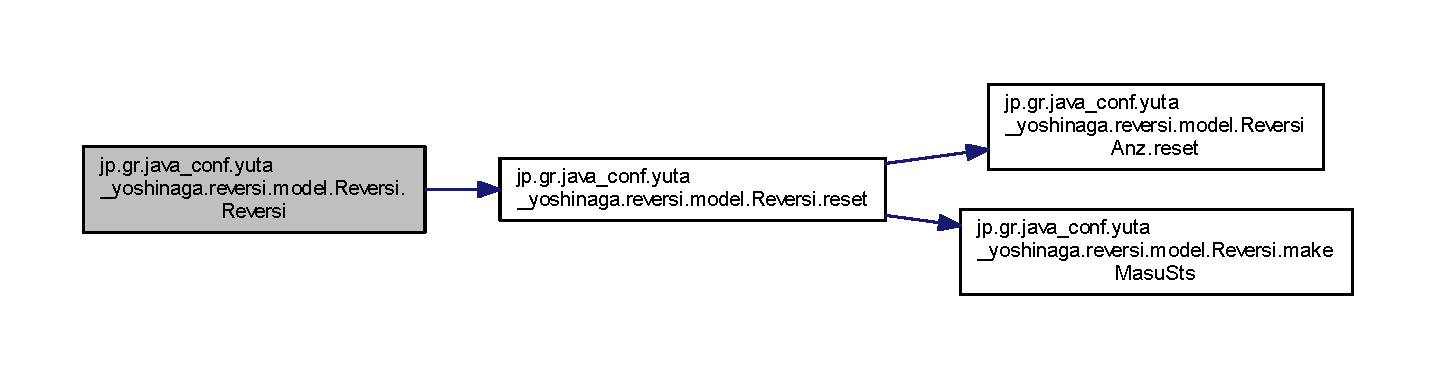
\includegraphics[width=350pt]{classjp_1_1gr_1_1java__conf_1_1yuta__yoshinaga_1_1reversi_1_1model_1_1_reversi_a22abbc9c1a2016388dafb08dc9a7b820_cgraph}
\end{center}
\end{figure}
\mbox{\Hypertarget{classjp_1_1gr_1_1java__conf_1_1yuta__yoshinaga_1_1reversi_1_1model_1_1_reversi_a26c832c23ff4e38dd2bcf990d05296d6}\label{classjp_1_1gr_1_1java__conf_1_1yuta__yoshinaga_1_1reversi_1_1model_1_1_reversi_a26c832c23ff4e38dd2bcf990d05296d6}} 
\index{jp\+::gr\+::java\+\_\+conf\+::yuta\+\_\+yoshinaga\+::reversi\+::model\+::\+Reversi@{jp\+::gr\+::java\+\_\+conf\+::yuta\+\_\+yoshinaga\+::reversi\+::model\+::\+Reversi}!Reversi@{Reversi}}
\index{Reversi@{Reversi}!jp\+::gr\+::java\+\_\+conf\+::yuta\+\_\+yoshinaga\+::reversi\+::model\+::\+Reversi@{jp\+::gr\+::java\+\_\+conf\+::yuta\+\_\+yoshinaga\+::reversi\+::model\+::\+Reversi}}
\subsubsection{\texorpdfstring{Reversi()}{Reversi()}\hspace{0.1cm}{\footnotesize\ttfamily [2/2]}}
{\footnotesize\ttfamily public jp.\+gr.\+java\+\_\+conf.\+yuta\+\_\+yoshinaga.\+reversi.\+model.\+Reversi.\+Reversi (\begin{DoxyParamCaption}{ }\end{DoxyParamCaption})}



コンストラクタ 

\begin{DoxyReturn}{Returns}
ありません 
\end{DoxyReturn}
\begin{DoxyAuthor}{Author}
Yuta Yoshinaga 
\end{DoxyAuthor}
\begin{DoxyDate}{Date}
2018.\+04.\+01 
\end{DoxyDate}


Definition at line 615 of file Reversi.\+java.



\subsection{Member Function Documentation}
\mbox{\Hypertarget{classjp_1_1gr_1_1java__conf_1_1yuta__yoshinaga_1_1reversi_1_1model_1_1_reversi_a43098c043d0424bb5e5e60db358a324d}\label{classjp_1_1gr_1_1java__conf_1_1yuta__yoshinaga_1_1reversi_1_1model_1_1_reversi_a43098c043d0424bb5e5e60db358a324d}} 
\index{jp\+::gr\+::java\+\_\+conf\+::yuta\+\_\+yoshinaga\+::reversi\+::model\+::\+Reversi@{jp\+::gr\+::java\+\_\+conf\+::yuta\+\_\+yoshinaga\+::reversi\+::model\+::\+Reversi}!Analysis\+Reversi@{Analysis\+Reversi}}
\index{Analysis\+Reversi@{Analysis\+Reversi}!jp\+::gr\+::java\+\_\+conf\+::yuta\+\_\+yoshinaga\+::reversi\+::model\+::\+Reversi@{jp\+::gr\+::java\+\_\+conf\+::yuta\+\_\+yoshinaga\+::reversi\+::model\+::\+Reversi}}
\subsubsection{\texorpdfstring{Analysis\+Reversi()}{AnalysisReversi()}}
{\footnotesize\ttfamily public void jp.\+gr.\+java\+\_\+conf.\+yuta\+\_\+yoshinaga.\+reversi.\+model.\+Reversi.\+Analysis\+Reversi (\begin{DoxyParamCaption}\item[{int}]{b\+Pass\+Ena,  }\item[{int}]{w\+Pass\+Ena }\end{DoxyParamCaption})}



解析を行う 


\begin{DoxyParams}[1]{Parameters}
\mbox{\tt in}  & {\em int} & b\+Pass\+Ena 1=黒パス有効 \\
\hline
\mbox{\tt in}  & {\em int} & w\+Pass\+Ena 1=白パス有効 \\
\hline
\end{DoxyParams}
\begin{DoxyReturn}{Returns}
ありません 
\end{DoxyReturn}
\begin{DoxyAuthor}{Author}
Yuta Yoshinaga 
\end{DoxyAuthor}
\begin{DoxyDate}{Date}
2018.\+04.\+01 
\end{DoxyDate}


Definition at line 1326 of file Reversi.\+java.



Referenced by jp.\+gr.\+java\+\_\+conf.\+yuta\+\_\+yoshinaga.\+reversi.\+model.\+Reversi\+Play.\+reset(), jp.\+gr.\+java\+\_\+conf.\+yuta\+\_\+yoshinaga.\+reversi.\+model.\+Reversi\+Play.\+reversi\+Play(), and jp.\+gr.\+java\+\_\+conf.\+yuta\+\_\+yoshinaga.\+reversi.\+model.\+Reversi\+Play.\+reversi\+Play\+Cpu().

Here is the call graph for this function\+:
\nopagebreak
\begin{figure}[H]
\begin{center}
\leavevmode
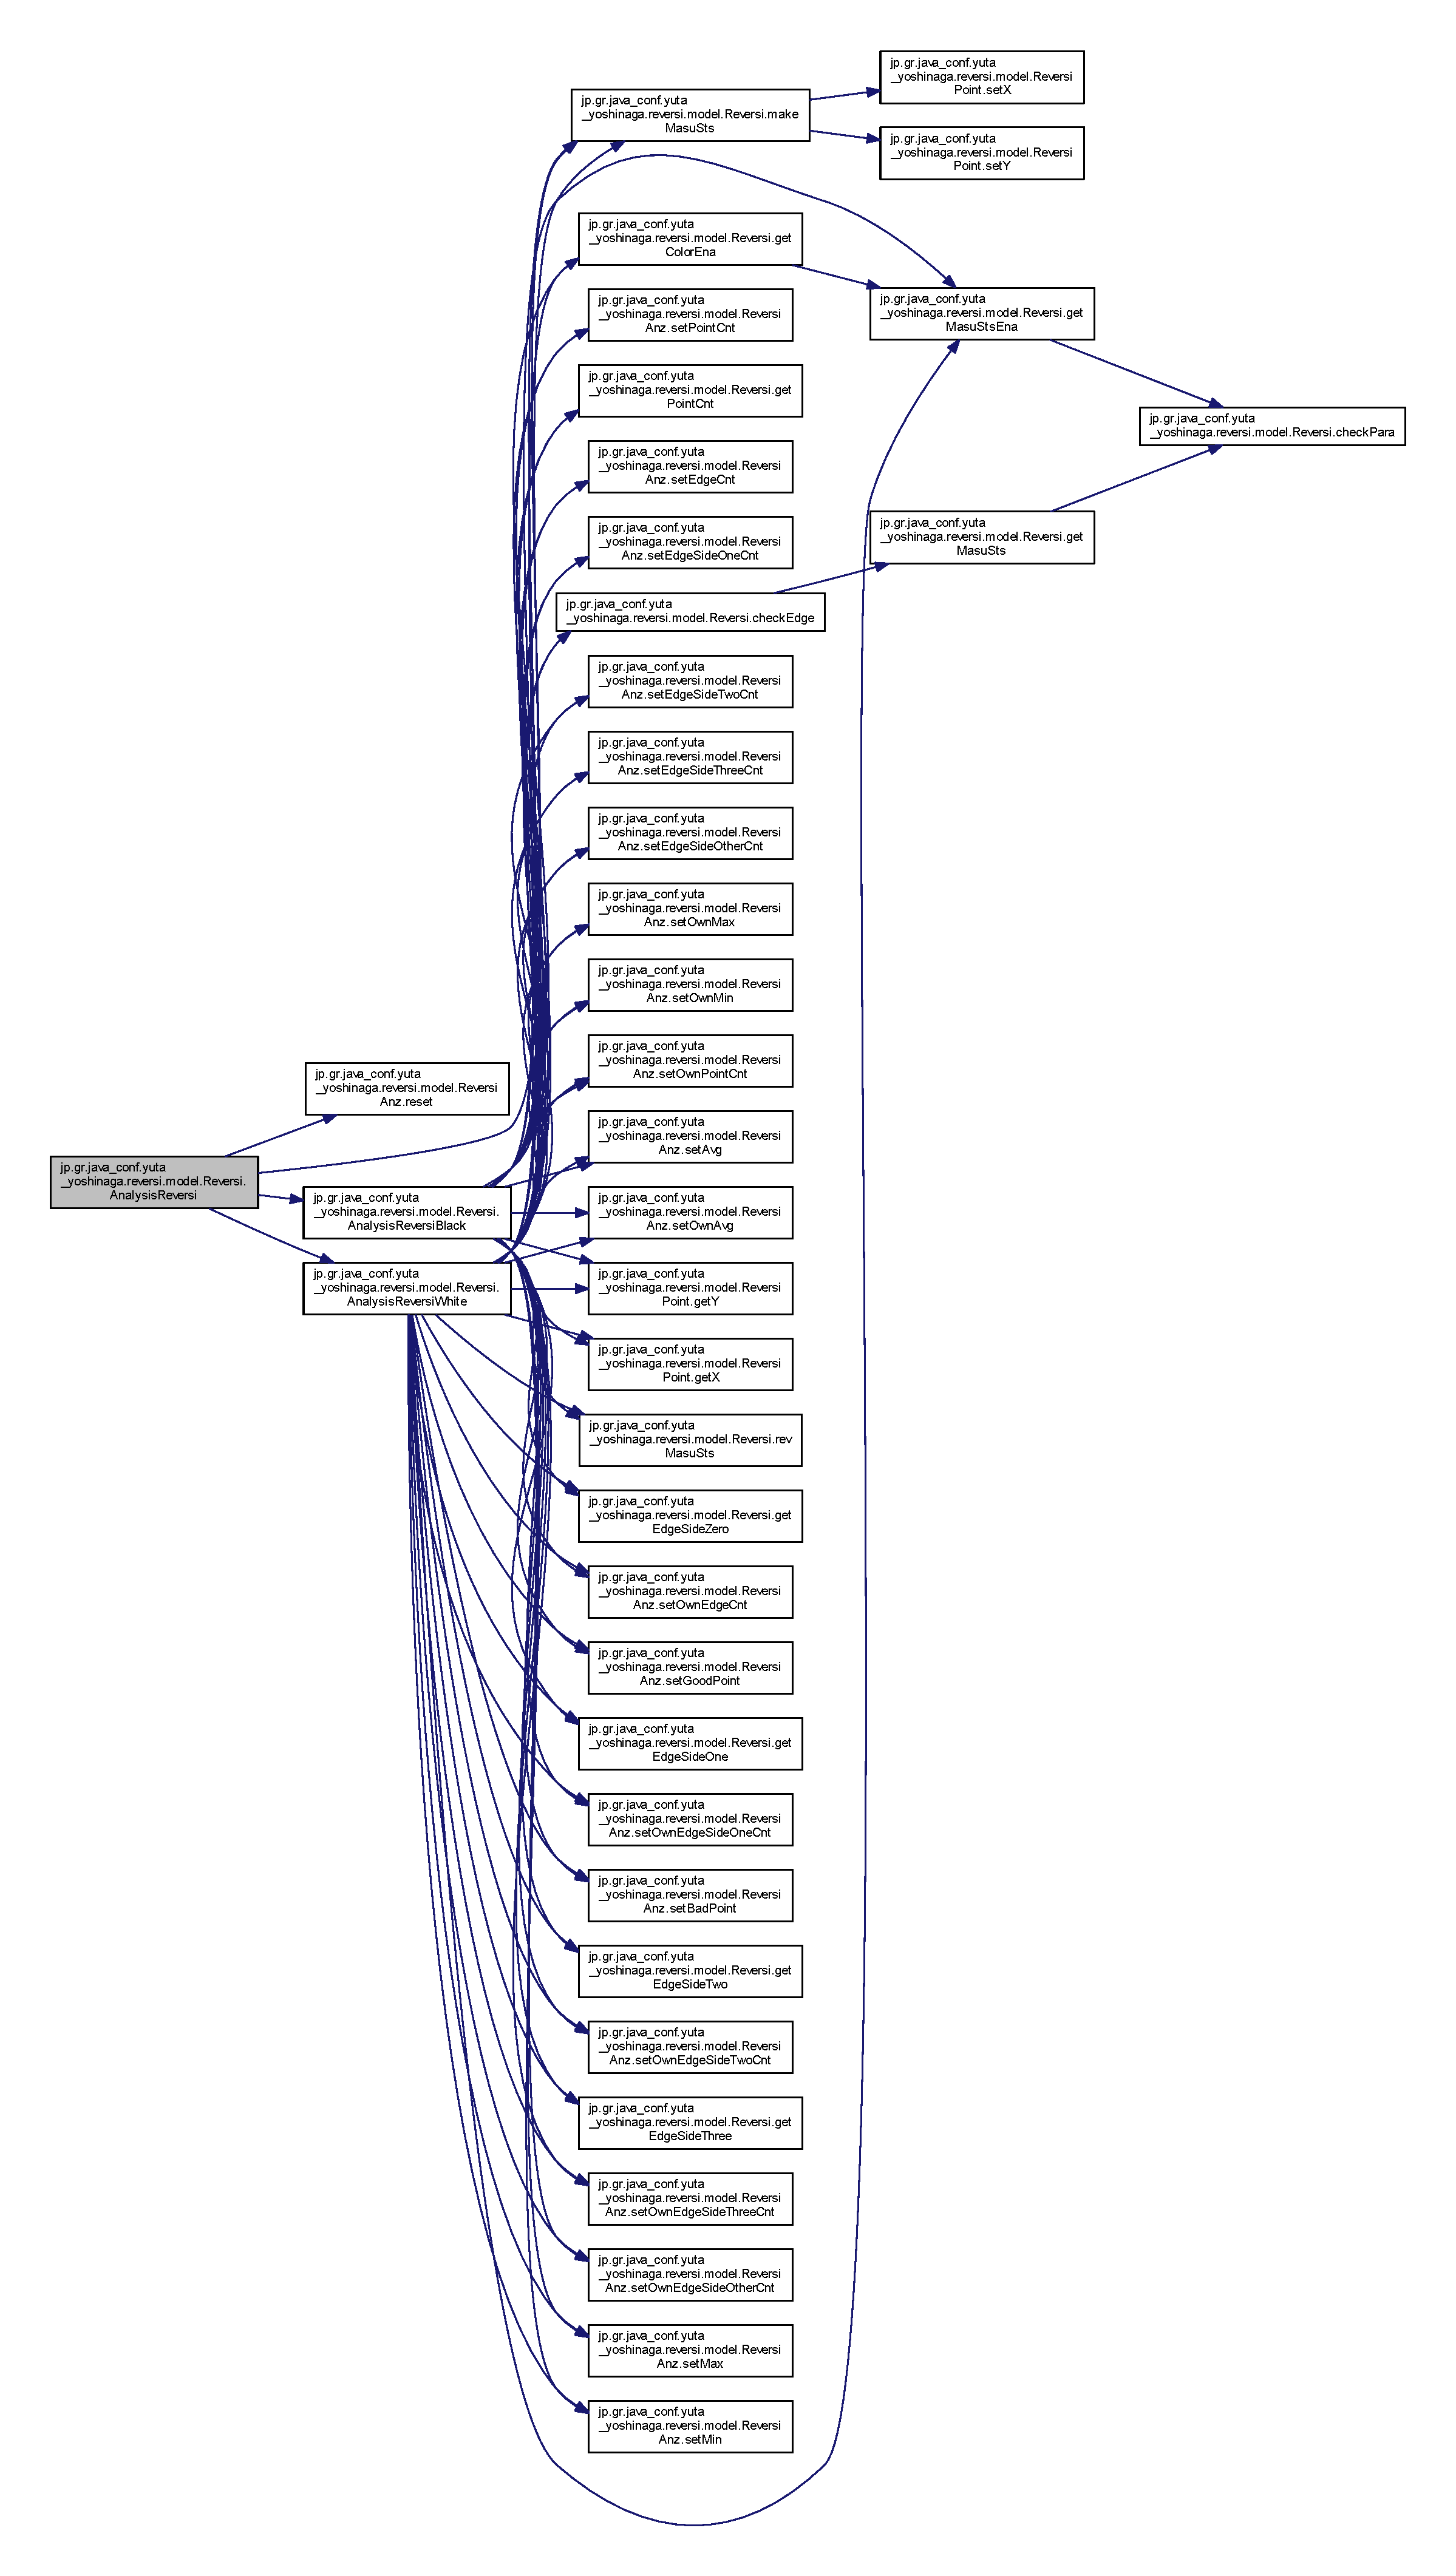
\includegraphics[height=550pt]{classjp_1_1gr_1_1java__conf_1_1yuta__yoshinaga_1_1reversi_1_1model_1_1_reversi_a43098c043d0424bb5e5e60db358a324d_cgraph}
\end{center}
\end{figure}
Here is the caller graph for this function\+:
\nopagebreak
\begin{figure}[H]
\begin{center}
\leavevmode
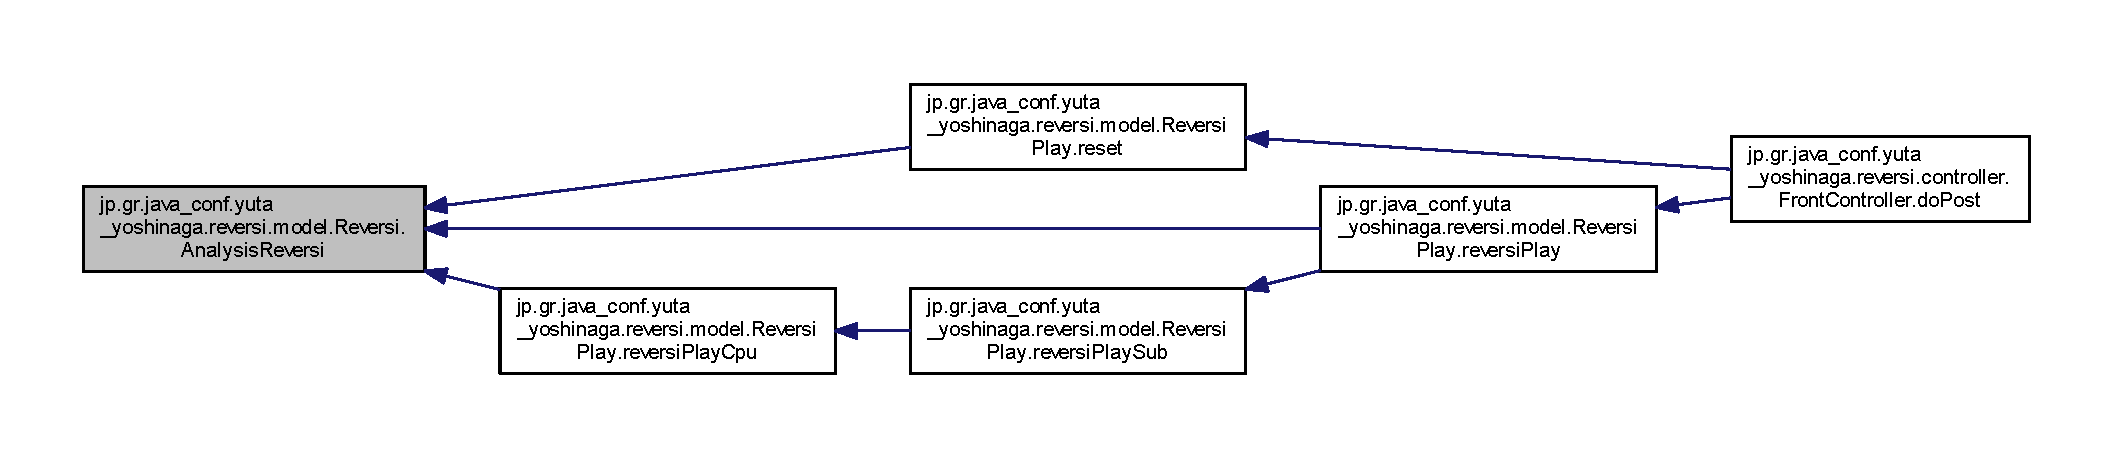
\includegraphics[width=350pt]{classjp_1_1gr_1_1java__conf_1_1yuta__yoshinaga_1_1reversi_1_1model_1_1_reversi_a43098c043d0424bb5e5e60db358a324d_icgraph}
\end{center}
\end{figure}
\mbox{\Hypertarget{classjp_1_1gr_1_1java__conf_1_1yuta__yoshinaga_1_1reversi_1_1model_1_1_reversi_adb74246f49150e02201766a1fa6cf732}\label{classjp_1_1gr_1_1java__conf_1_1yuta__yoshinaga_1_1reversi_1_1model_1_1_reversi_adb74246f49150e02201766a1fa6cf732}} 
\index{jp\+::gr\+::java\+\_\+conf\+::yuta\+\_\+yoshinaga\+::reversi\+::model\+::\+Reversi@{jp\+::gr\+::java\+\_\+conf\+::yuta\+\_\+yoshinaga\+::reversi\+::model\+::\+Reversi}!Analysis\+Reversi\+Black@{Analysis\+Reversi\+Black}}
\index{Analysis\+Reversi\+Black@{Analysis\+Reversi\+Black}!jp\+::gr\+::java\+\_\+conf\+::yuta\+\_\+yoshinaga\+::reversi\+::model\+::\+Reversi@{jp\+::gr\+::java\+\_\+conf\+::yuta\+\_\+yoshinaga\+::reversi\+::model\+::\+Reversi}}
\subsubsection{\texorpdfstring{Analysis\+Reversi\+Black()}{AnalysisReversiBlack()}}
{\footnotesize\ttfamily private void jp.\+gr.\+java\+\_\+conf.\+yuta\+\_\+yoshinaga.\+reversi.\+model.\+Reversi.\+Analysis\+Reversi\+Black (\begin{DoxyParamCaption}{ }\end{DoxyParamCaption})\hspace{0.3cm}{\ttfamily [private]}}



解析を行う(黒) 

\begin{DoxyReturn}{Returns}
ありません 
\end{DoxyReturn}
\begin{DoxyAuthor}{Author}
Yuta Yoshinaga 
\end{DoxyAuthor}
\begin{DoxyDate}{Date}
2018.\+04.\+01 
\end{DoxyDate}


Definition at line 1044 of file Reversi.\+java.



Referenced by jp.\+gr.\+java\+\_\+conf.\+yuta\+\_\+yoshinaga.\+reversi.\+model.\+Reversi.\+Analysis\+Reversi().

Here is the call graph for this function\+:
\nopagebreak
\begin{figure}[H]
\begin{center}
\leavevmode
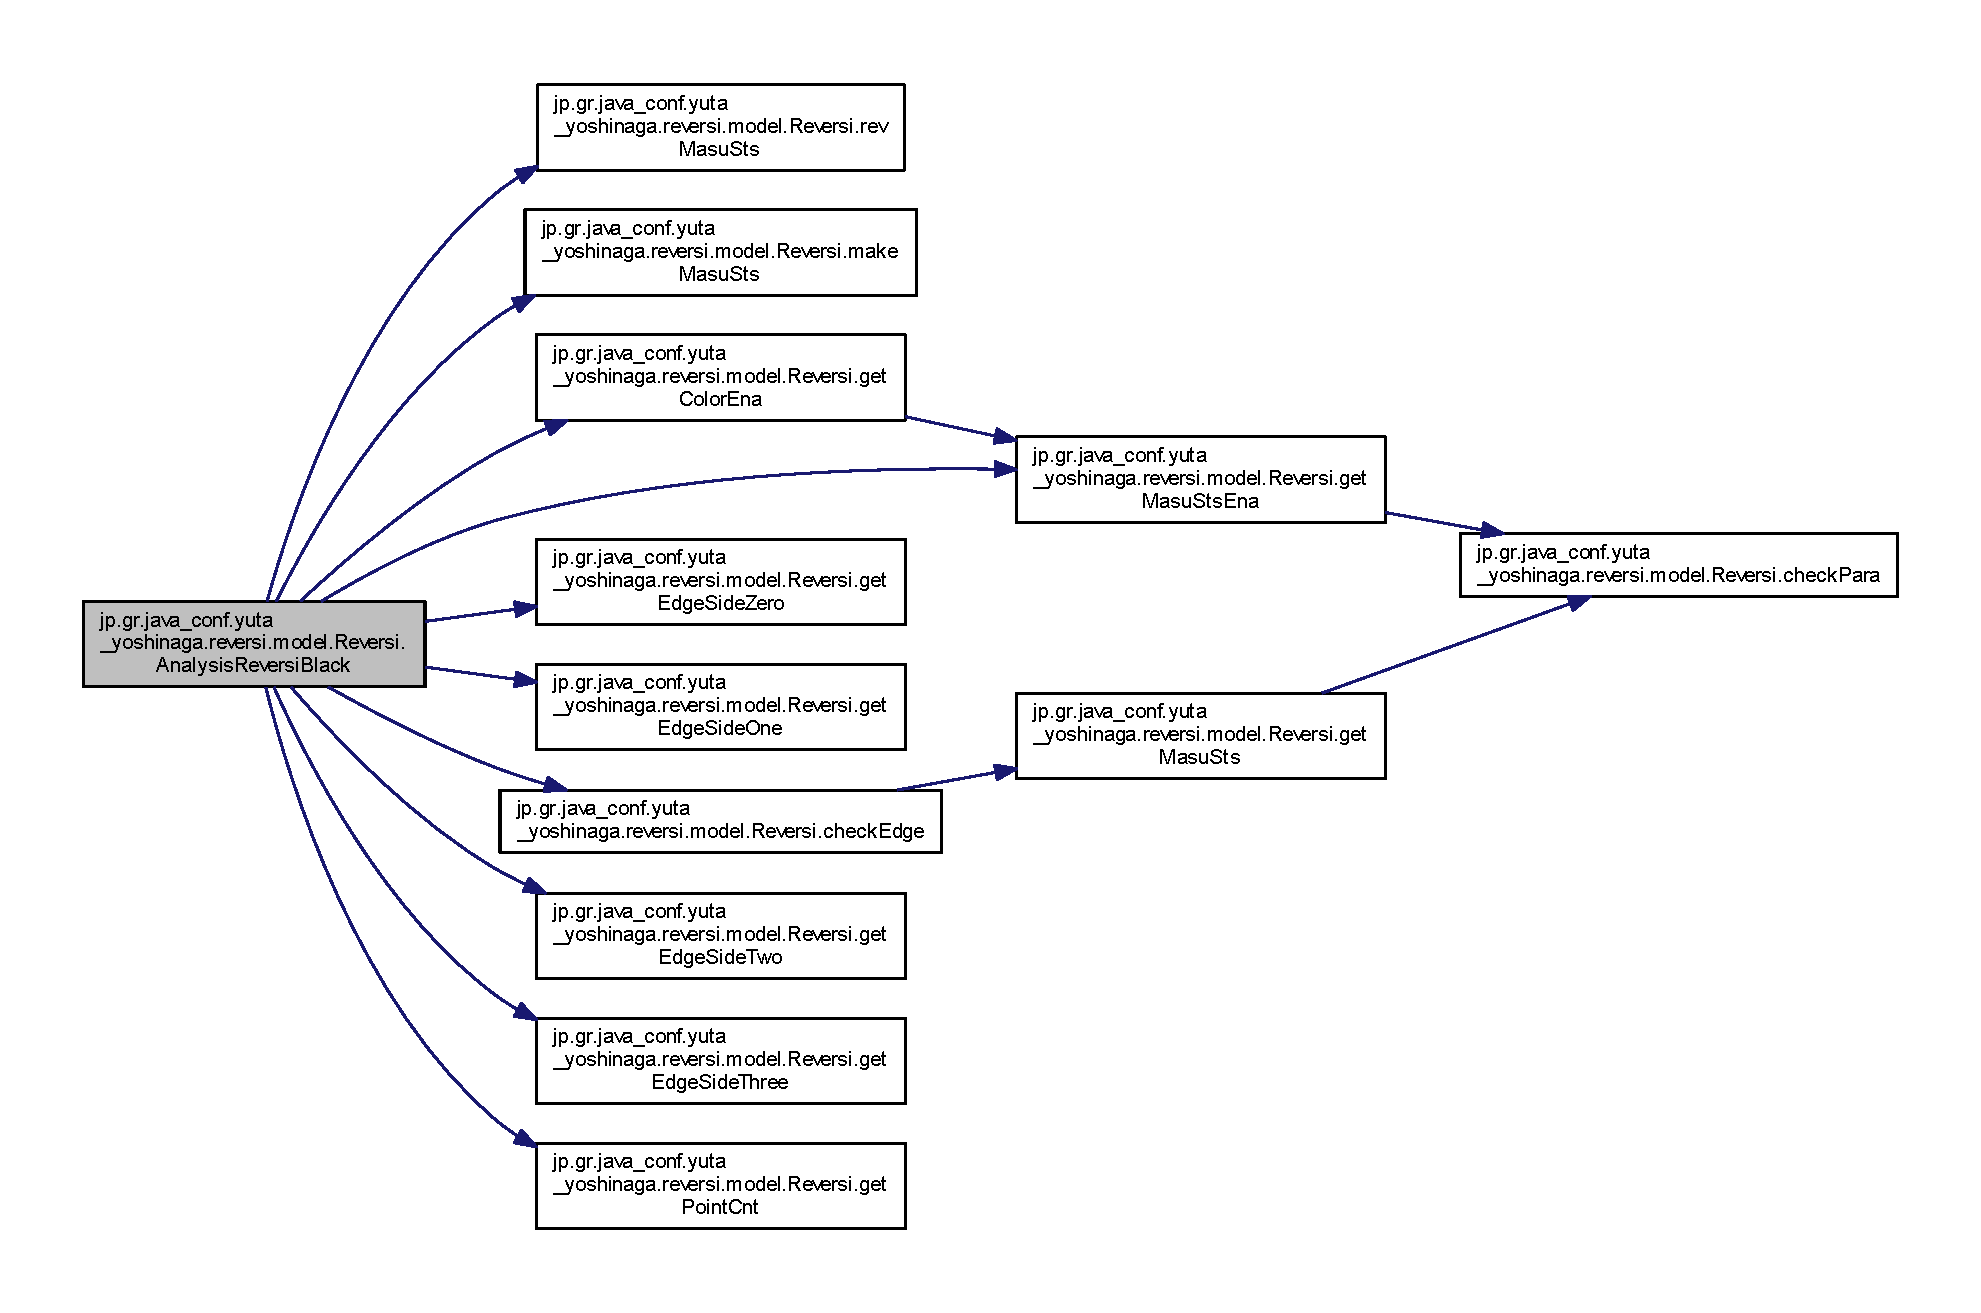
\includegraphics[height=550pt]{classjp_1_1gr_1_1java__conf_1_1yuta__yoshinaga_1_1reversi_1_1model_1_1_reversi_adb74246f49150e02201766a1fa6cf732_cgraph}
\end{center}
\end{figure}
Here is the caller graph for this function\+:
\nopagebreak
\begin{figure}[H]
\begin{center}
\leavevmode
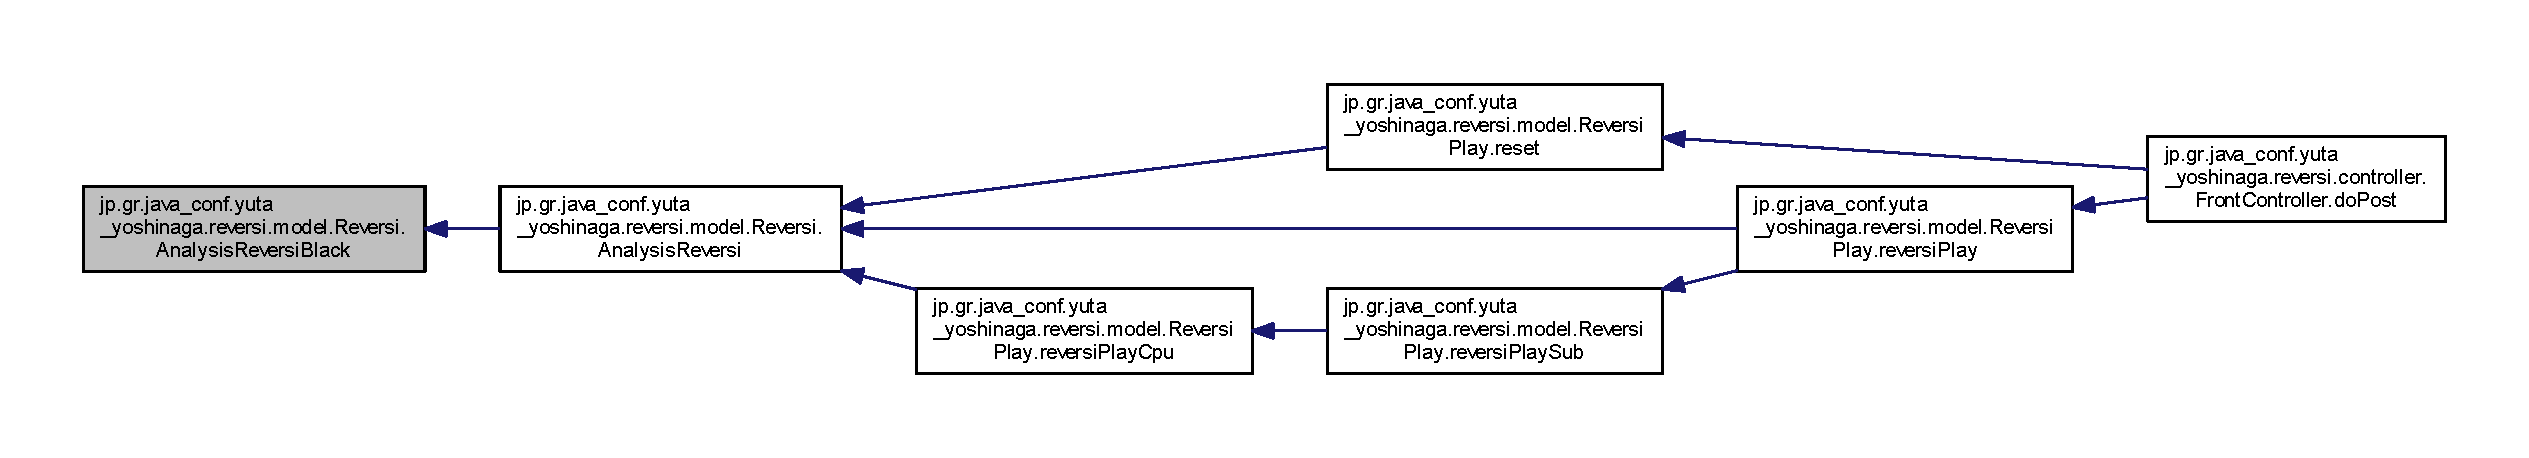
\includegraphics[width=350pt]{classjp_1_1gr_1_1java__conf_1_1yuta__yoshinaga_1_1reversi_1_1model_1_1_reversi_adb74246f49150e02201766a1fa6cf732_icgraph}
\end{center}
\end{figure}
\mbox{\Hypertarget{classjp_1_1gr_1_1java__conf_1_1yuta__yoshinaga_1_1reversi_1_1model_1_1_reversi_a519adbc5ec3bf5433fdb79bf8049cc75}\label{classjp_1_1gr_1_1java__conf_1_1yuta__yoshinaga_1_1reversi_1_1model_1_1_reversi_a519adbc5ec3bf5433fdb79bf8049cc75}} 
\index{jp\+::gr\+::java\+\_\+conf\+::yuta\+\_\+yoshinaga\+::reversi\+::model\+::\+Reversi@{jp\+::gr\+::java\+\_\+conf\+::yuta\+\_\+yoshinaga\+::reversi\+::model\+::\+Reversi}!Analysis\+Reversi\+White@{Analysis\+Reversi\+White}}
\index{Analysis\+Reversi\+White@{Analysis\+Reversi\+White}!jp\+::gr\+::java\+\_\+conf\+::yuta\+\_\+yoshinaga\+::reversi\+::model\+::\+Reversi@{jp\+::gr\+::java\+\_\+conf\+::yuta\+\_\+yoshinaga\+::reversi\+::model\+::\+Reversi}}
\subsubsection{\texorpdfstring{Analysis\+Reversi\+White()}{AnalysisReversiWhite()}}
{\footnotesize\ttfamily private void jp.\+gr.\+java\+\_\+conf.\+yuta\+\_\+yoshinaga.\+reversi.\+model.\+Reversi.\+Analysis\+Reversi\+White (\begin{DoxyParamCaption}{ }\end{DoxyParamCaption})\hspace{0.3cm}{\ttfamily [private]}}



解析を行う(白) 

\begin{DoxyReturn}{Returns}
ありません 
\end{DoxyReturn}
\begin{DoxyAuthor}{Author}
Yuta Yoshinaga 
\end{DoxyAuthor}
\begin{DoxyDate}{Date}
2018.\+04.\+01 
\end{DoxyDate}


Definition at line 1184 of file Reversi.\+java.



Referenced by jp.\+gr.\+java\+\_\+conf.\+yuta\+\_\+yoshinaga.\+reversi.\+model.\+Reversi.\+Analysis\+Reversi().

Here is the call graph for this function\+:
\nopagebreak
\begin{figure}[H]
\begin{center}
\leavevmode
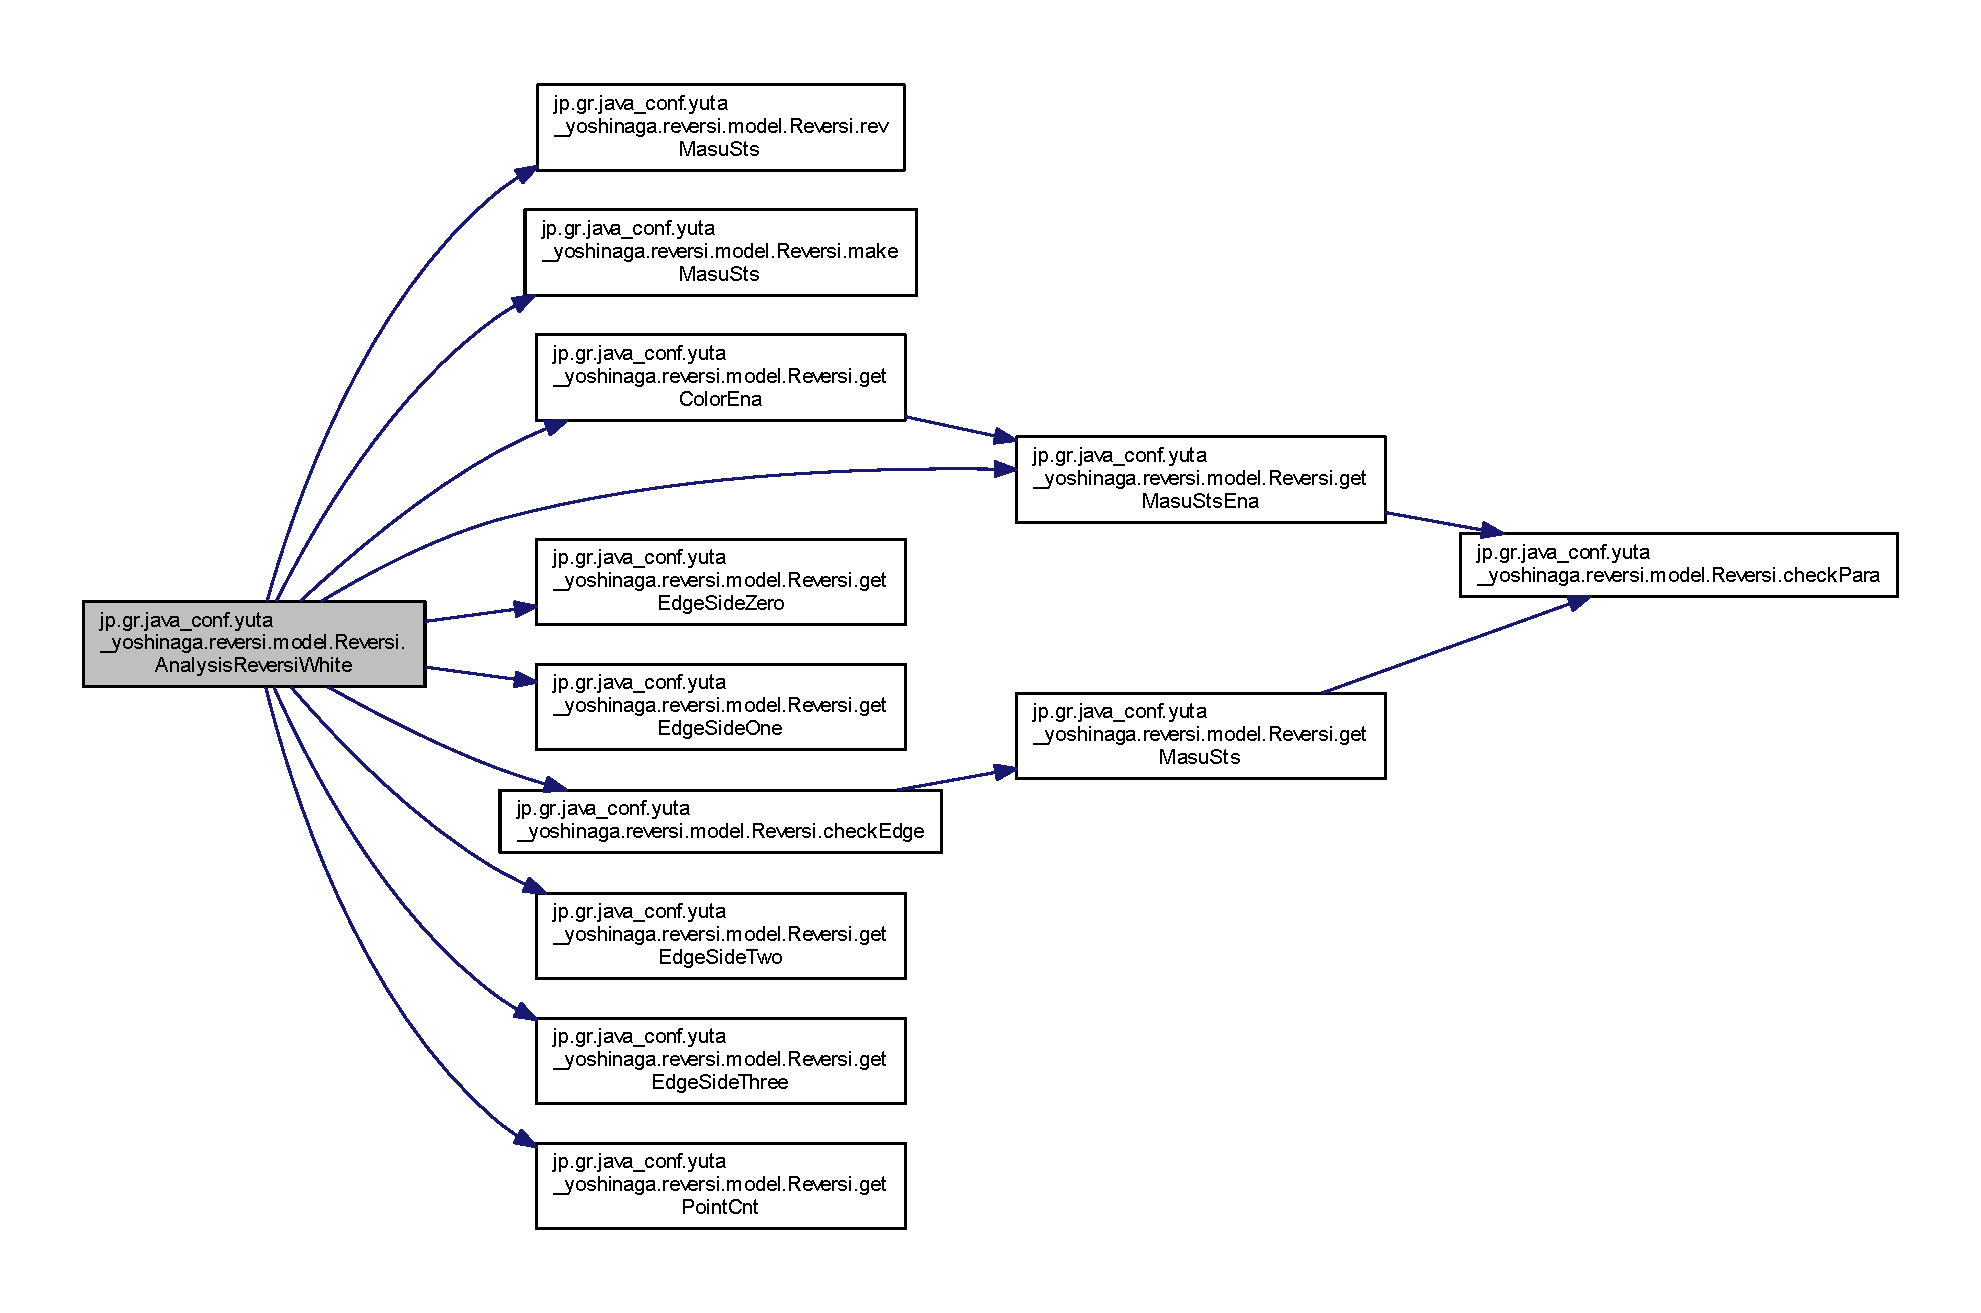
\includegraphics[height=550pt]{classjp_1_1gr_1_1java__conf_1_1yuta__yoshinaga_1_1reversi_1_1model_1_1_reversi_a519adbc5ec3bf5433fdb79bf8049cc75_cgraph}
\end{center}
\end{figure}
Here is the caller graph for this function\+:
\nopagebreak
\begin{figure}[H]
\begin{center}
\leavevmode
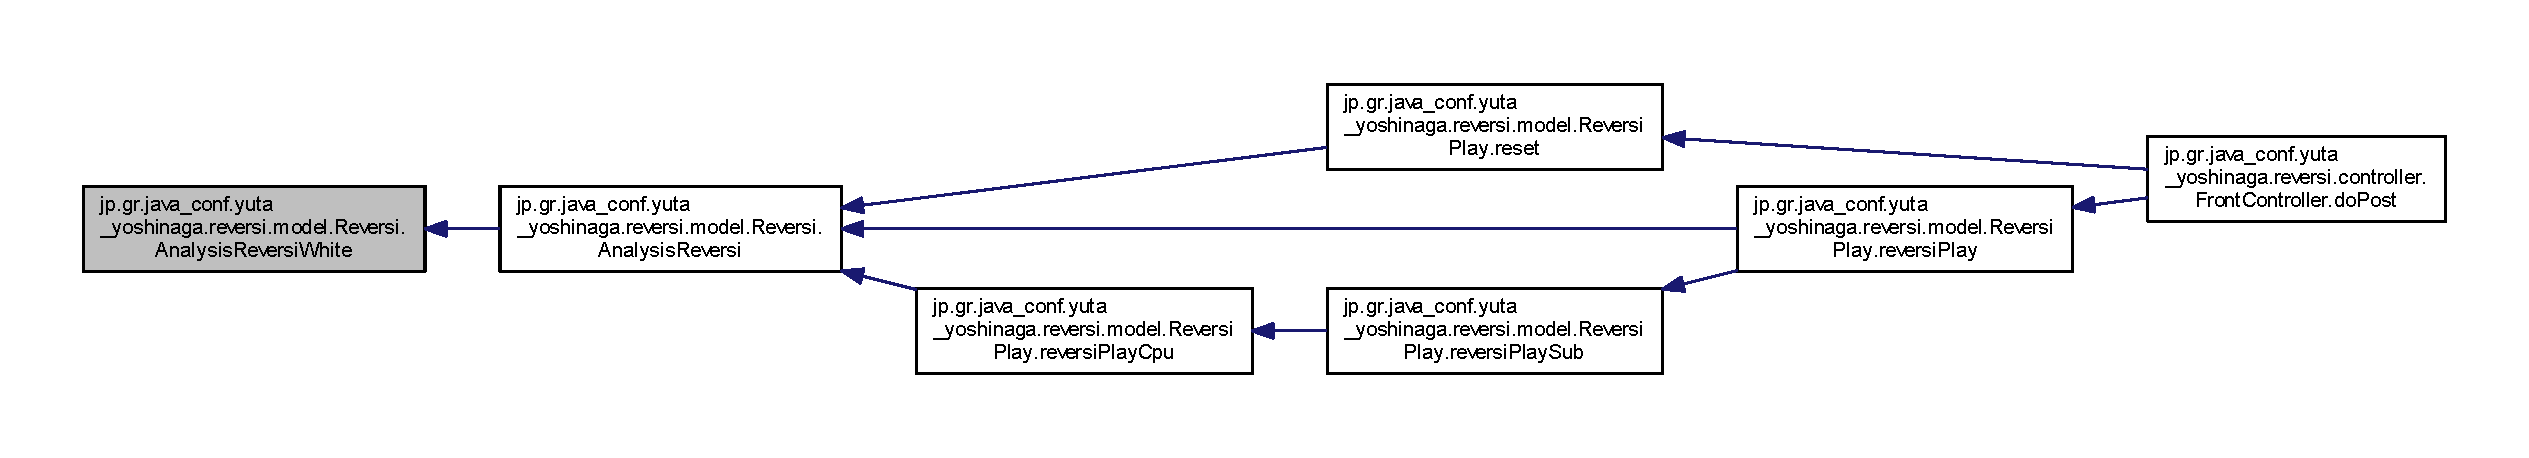
\includegraphics[width=350pt]{classjp_1_1gr_1_1java__conf_1_1yuta__yoshinaga_1_1reversi_1_1model_1_1_reversi_a519adbc5ec3bf5433fdb79bf8049cc75_icgraph}
\end{center}
\end{figure}
\mbox{\Hypertarget{classjp_1_1gr_1_1java__conf_1_1yuta__yoshinaga_1_1reversi_1_1model_1_1_reversi_a4874c6523adfdfd42dfbd625f5e3fe7a}\label{classjp_1_1gr_1_1java__conf_1_1yuta__yoshinaga_1_1reversi_1_1model_1_1_reversi_a4874c6523adfdfd42dfbd625f5e3fe7a}} 
\index{jp\+::gr\+::java\+\_\+conf\+::yuta\+\_\+yoshinaga\+::reversi\+::model\+::\+Reversi@{jp\+::gr\+::java\+\_\+conf\+::yuta\+\_\+yoshinaga\+::reversi\+::model\+::\+Reversi}!check\+Edge@{check\+Edge}}
\index{check\+Edge@{check\+Edge}!jp\+::gr\+::java\+\_\+conf\+::yuta\+\_\+yoshinaga\+::reversi\+::model\+::\+Reversi@{jp\+::gr\+::java\+\_\+conf\+::yuta\+\_\+yoshinaga\+::reversi\+::model\+::\+Reversi}}
\subsubsection{\texorpdfstring{check\+Edge()}{checkEdge()}}
{\footnotesize\ttfamily public int jp.\+gr.\+java\+\_\+conf.\+yuta\+\_\+yoshinaga.\+reversi.\+model.\+Reversi.\+check\+Edge (\begin{DoxyParamCaption}\item[{int}]{color,  }\item[{int}]{y,  }\item[{int}]{x }\end{DoxyParamCaption})}



角の隣に置いても角を取られないマス検索 


\begin{DoxyParams}[1]{Parameters}
\mbox{\tt in}  & {\em int} & color 色 \\
\hline
\mbox{\tt in}  & {\em int} & y Y座標 \\
\hline
\mbox{\tt in}  & {\em int} & x X座標 \\
\hline
\end{DoxyParams}
\begin{DoxyReturn}{Returns}
0 \+: 取られる それ以外 \+: 取られない 
\end{DoxyReturn}
\begin{DoxyAuthor}{Author}
Yuta Yoshinaga 
\end{DoxyAuthor}
\begin{DoxyDate}{Date}
2018.\+04.\+01 
\end{DoxyDate}


Definition at line 1693 of file Reversi.\+java.



Referenced by jp.\+gr.\+java\+\_\+conf.\+yuta\+\_\+yoshinaga.\+reversi.\+model.\+Reversi.\+Analysis\+Reversi\+Black(), jp.\+gr.\+java\+\_\+conf.\+yuta\+\_\+yoshinaga.\+reversi.\+model.\+Reversi.\+Analysis\+Reversi\+White(), and jp.\+gr.\+java\+\_\+conf.\+yuta\+\_\+yoshinaga.\+reversi.\+model.\+Reversi\+Play.\+reversi\+Play\+Cpu().

Here is the call graph for this function\+:
\nopagebreak
\begin{figure}[H]
\begin{center}
\leavevmode
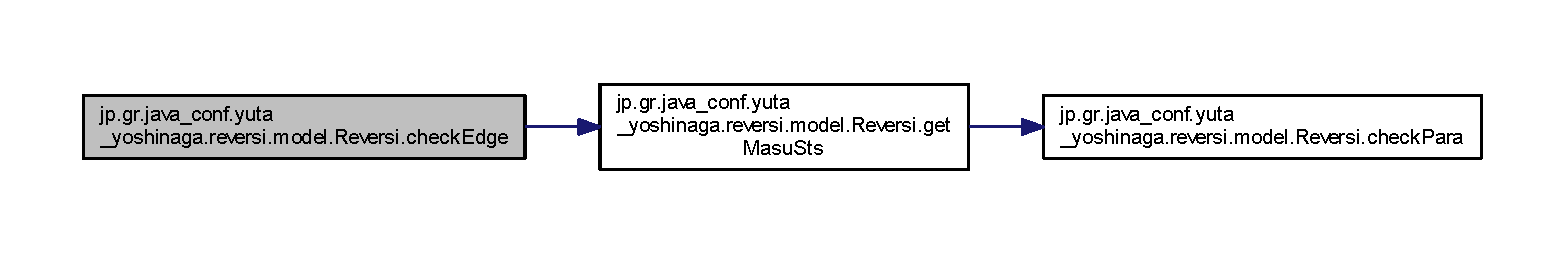
\includegraphics[width=350pt]{classjp_1_1gr_1_1java__conf_1_1yuta__yoshinaga_1_1reversi_1_1model_1_1_reversi_a4874c6523adfdfd42dfbd625f5e3fe7a_cgraph}
\end{center}
\end{figure}
Here is the caller graph for this function\+:
\nopagebreak
\begin{figure}[H]
\begin{center}
\leavevmode
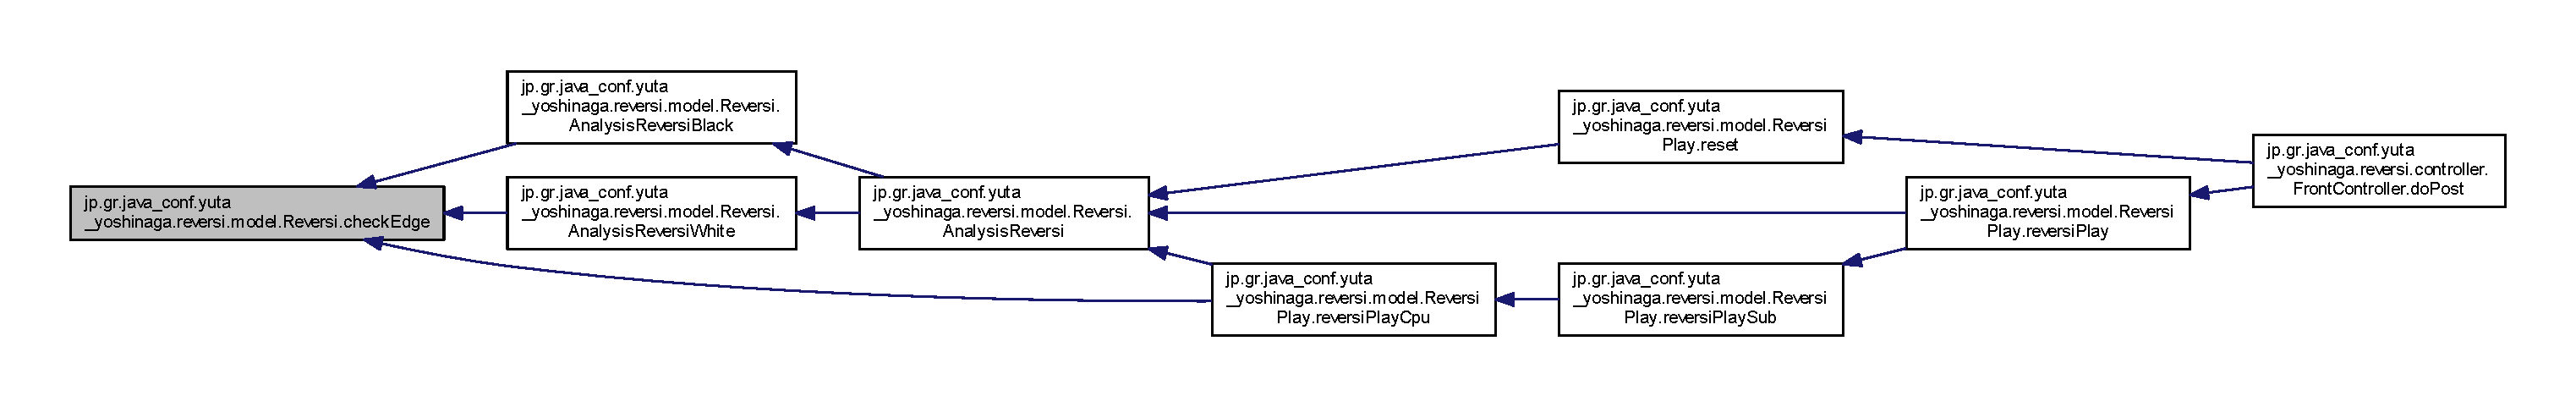
\includegraphics[width=350pt]{classjp_1_1gr_1_1java__conf_1_1yuta__yoshinaga_1_1reversi_1_1model_1_1_reversi_a4874c6523adfdfd42dfbd625f5e3fe7a_icgraph}
\end{center}
\end{figure}
\mbox{\Hypertarget{classjp_1_1gr_1_1java__conf_1_1yuta__yoshinaga_1_1reversi_1_1model_1_1_reversi_afbad8b2c3b2423a7490f9a3b636584d3}\label{classjp_1_1gr_1_1java__conf_1_1yuta__yoshinaga_1_1reversi_1_1model_1_1_reversi_afbad8b2c3b2423a7490f9a3b636584d3}} 
\index{jp\+::gr\+::java\+\_\+conf\+::yuta\+\_\+yoshinaga\+::reversi\+::model\+::\+Reversi@{jp\+::gr\+::java\+\_\+conf\+::yuta\+\_\+yoshinaga\+::reversi\+::model\+::\+Reversi}!check\+Para@{check\+Para}}
\index{check\+Para@{check\+Para}!jp\+::gr\+::java\+\_\+conf\+::yuta\+\_\+yoshinaga\+::reversi\+::model\+::\+Reversi@{jp\+::gr\+::java\+\_\+conf\+::yuta\+\_\+yoshinaga\+::reversi\+::model\+::\+Reversi}}
\subsubsection{\texorpdfstring{check\+Para()}{checkPara()}}
{\footnotesize\ttfamily private int jp.\+gr.\+java\+\_\+conf.\+yuta\+\_\+yoshinaga.\+reversi.\+model.\+Reversi.\+check\+Para (\begin{DoxyParamCaption}\item[{int}]{para,  }\item[{int}]{min,  }\item[{int}]{max }\end{DoxyParamCaption})\hspace{0.3cm}{\ttfamily [private]}}



パラメーター範囲チェック 


\begin{DoxyParams}[1]{Parameters}
\mbox{\tt in}  & {\em int} & para チェックパラメーター \\
\hline
\mbox{\tt in}  & {\em int} & min パラメーター最小値 \\
\hline
\mbox{\tt in}  & {\em int} & max パラメーター最大値 \\
\hline
\end{DoxyParams}
\begin{DoxyReturn}{Returns}
0 \+: 成功 それ以外 \+: 失敗 
\end{DoxyReturn}
\begin{DoxyAuthor}{Author}
Yuta Yoshinaga 
\end{DoxyAuthor}
\begin{DoxyDate}{Date}
2018.\+04.\+01 
\end{DoxyDate}


Definition at line 1029 of file Reversi.\+java.



Referenced by jp.\+gr.\+java\+\_\+conf.\+yuta\+\_\+yoshinaga.\+reversi.\+model.\+Reversi.\+get\+Bet\+Cnt(), jp.\+gr.\+java\+\_\+conf.\+yuta\+\_\+yoshinaga.\+reversi.\+model.\+Reversi.\+get\+History(), jp.\+gr.\+java\+\_\+conf.\+yuta\+\_\+yoshinaga.\+reversi.\+model.\+Reversi.\+get\+Masu\+Sts(), jp.\+gr.\+java\+\_\+conf.\+yuta\+\_\+yoshinaga.\+reversi.\+model.\+Reversi.\+get\+Masu\+Sts\+Cnt(), jp.\+gr.\+java\+\_\+conf.\+yuta\+\_\+yoshinaga.\+reversi.\+model.\+Reversi.\+get\+Masu\+Sts\+Ena(), jp.\+gr.\+java\+\_\+conf.\+yuta\+\_\+yoshinaga.\+reversi.\+model.\+Reversi.\+get\+Masu\+Sts\+Old(), jp.\+gr.\+java\+\_\+conf.\+yuta\+\_\+yoshinaga.\+reversi.\+model.\+Reversi.\+get\+Point(), jp.\+gr.\+java\+\_\+conf.\+yuta\+\_\+yoshinaga.\+reversi.\+model.\+Reversi.\+get\+Point\+Anz(), and jp.\+gr.\+java\+\_\+conf.\+yuta\+\_\+yoshinaga.\+reversi.\+model.\+Reversi.\+set\+Masu\+Cnt().

Here is the caller graph for this function\+:
\nopagebreak
\begin{figure}[H]
\begin{center}
\leavevmode
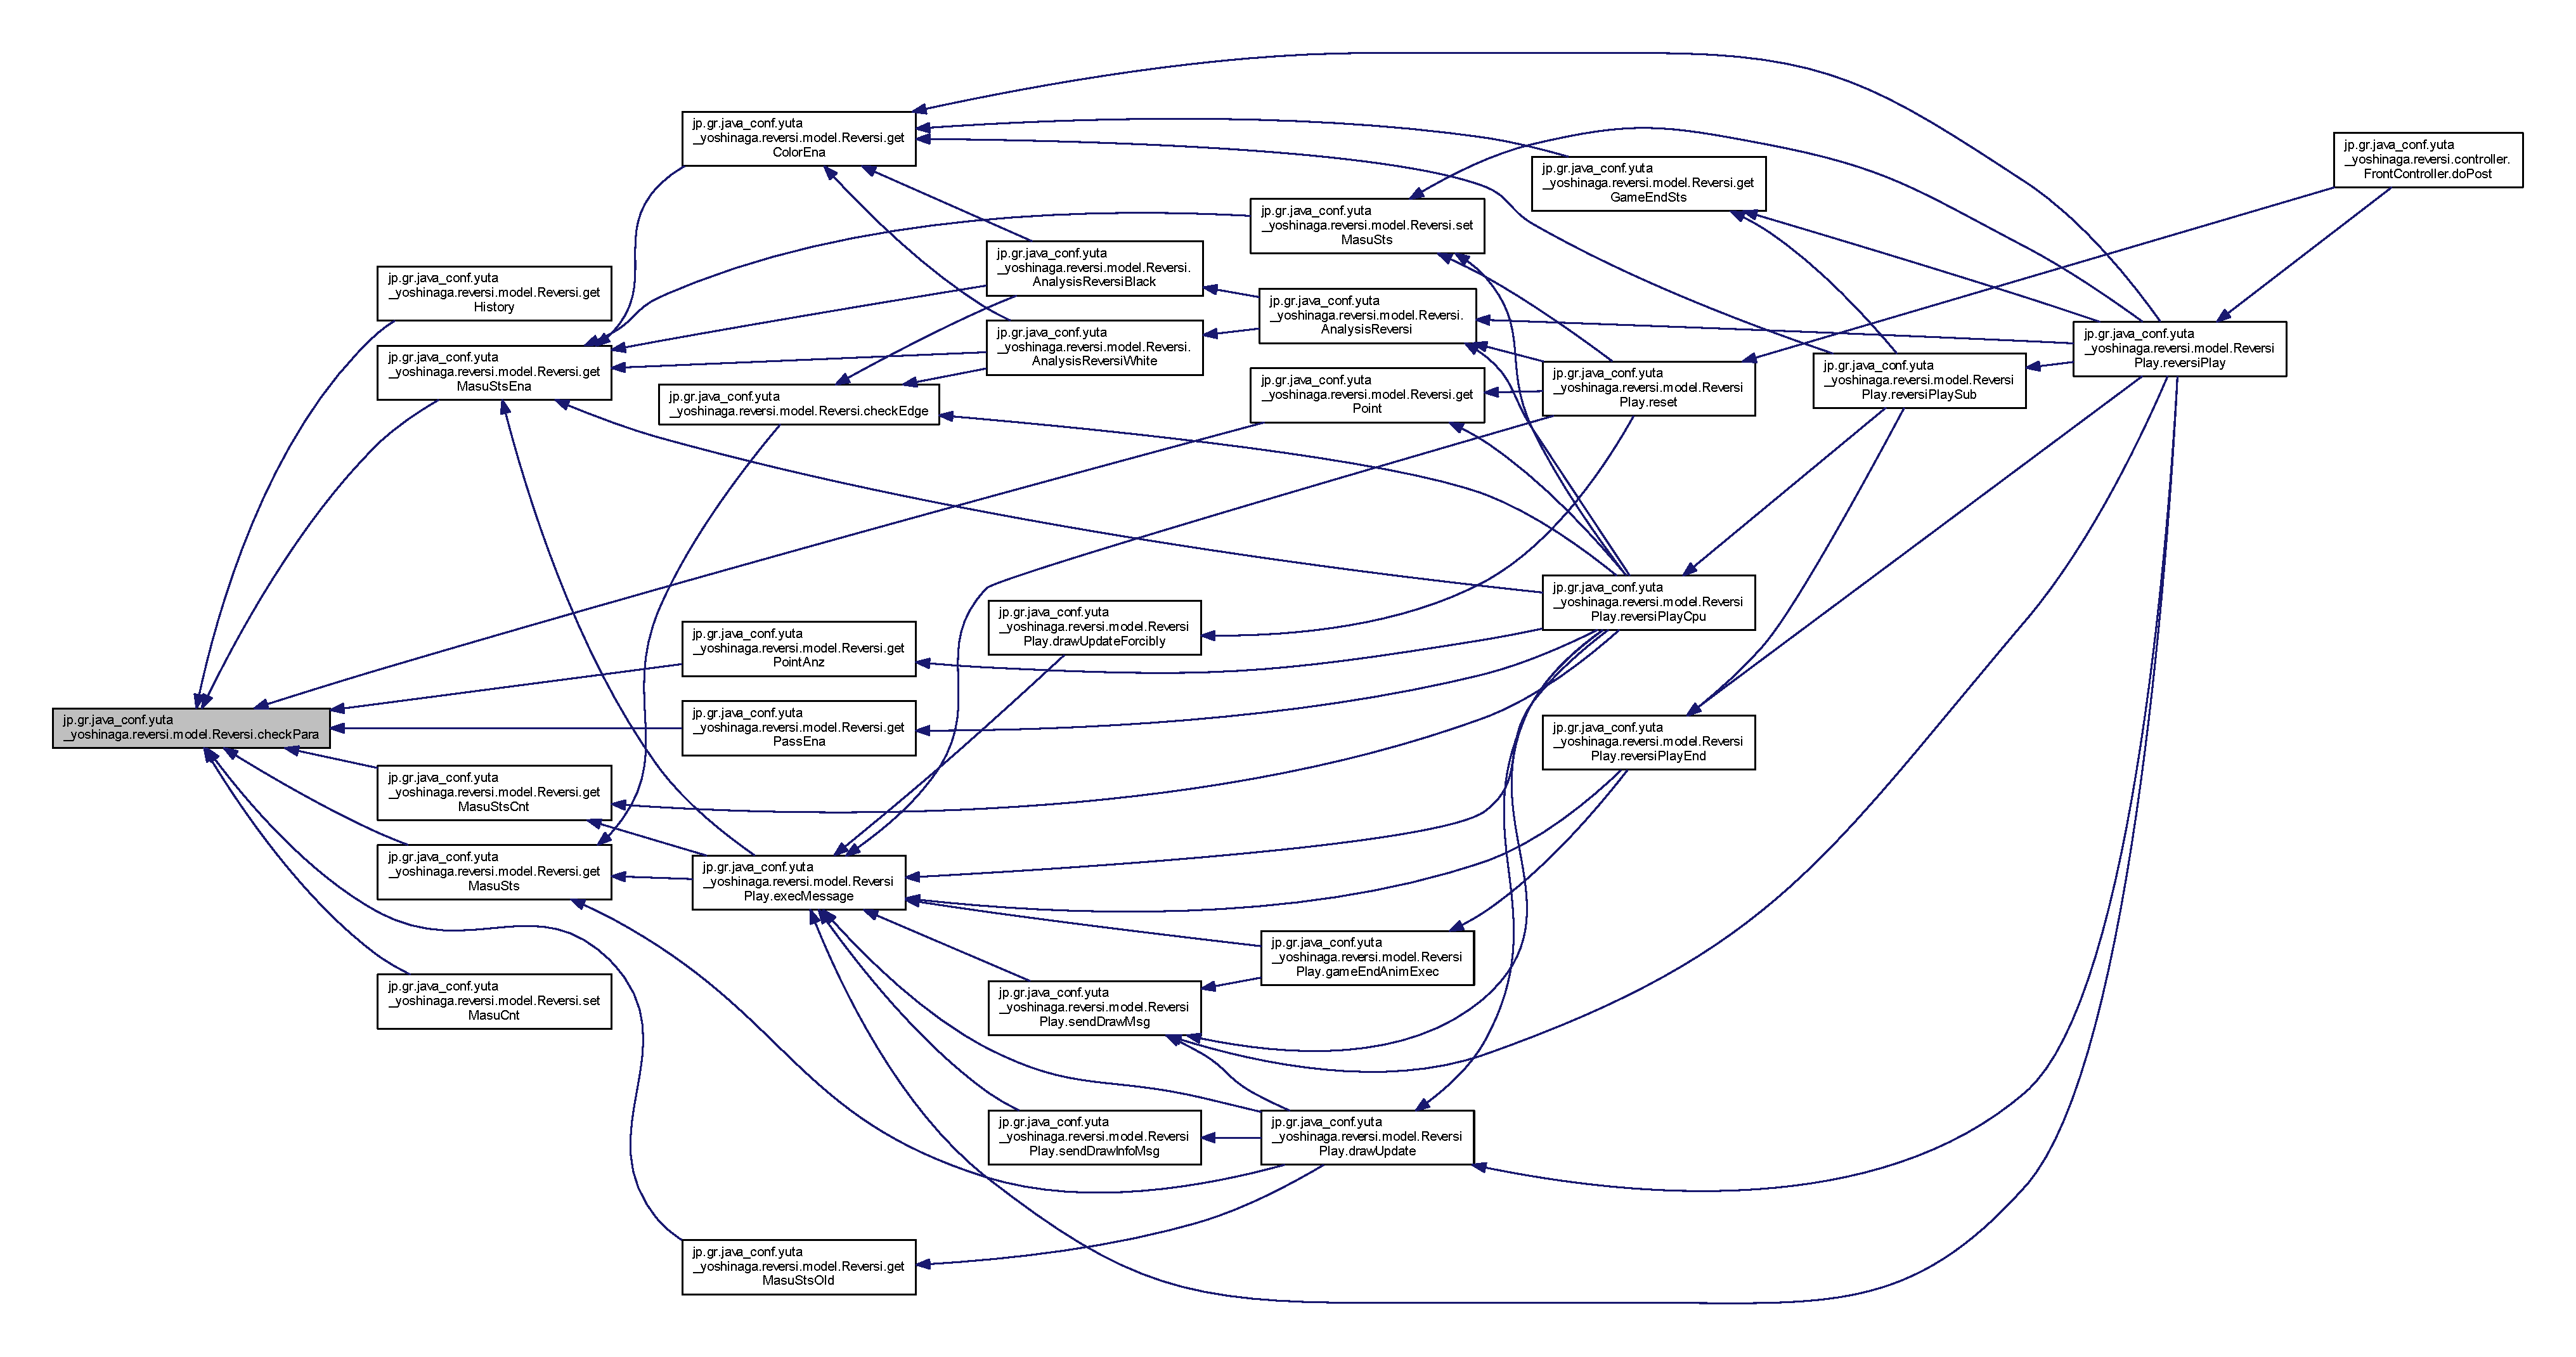
\includegraphics[width=350pt]{classjp_1_1gr_1_1java__conf_1_1yuta__yoshinaga_1_1reversi_1_1model_1_1_reversi_afbad8b2c3b2423a7490f9a3b636584d3_icgraph}
\end{center}
\end{figure}
\mbox{\Hypertarget{classjp_1_1gr_1_1java__conf_1_1yuta__yoshinaga_1_1reversi_1_1model_1_1_reversi_a9f826e110ec3298a6bc5d6987a94519c}\label{classjp_1_1gr_1_1java__conf_1_1yuta__yoshinaga_1_1reversi_1_1model_1_1_reversi_a9f826e110ec3298a6bc5d6987a94519c}} 
\index{jp\+::gr\+::java\+\_\+conf\+::yuta\+\_\+yoshinaga\+::reversi\+::model\+::\+Reversi@{jp\+::gr\+::java\+\_\+conf\+::yuta\+\_\+yoshinaga\+::reversi\+::model\+::\+Reversi}!get\+Bet\+Cnt@{get\+Bet\+Cnt}}
\index{get\+Bet\+Cnt@{get\+Bet\+Cnt}!jp\+::gr\+::java\+\_\+conf\+::yuta\+\_\+yoshinaga\+::reversi\+::model\+::\+Reversi@{jp\+::gr\+::java\+\_\+conf\+::yuta\+\_\+yoshinaga\+::reversi\+::model\+::\+Reversi}}
\subsubsection{\texorpdfstring{get\+Bet\+Cnt()}{getBetCnt()}}
{\footnotesize\ttfamily public int jp.\+gr.\+java\+\_\+conf.\+yuta\+\_\+yoshinaga.\+reversi.\+model.\+Reversi.\+get\+Bet\+Cnt (\begin{DoxyParamCaption}\item[{int}]{color }\end{DoxyParamCaption})}



コマ数取得 

パス判定


\begin{DoxyParams}[1]{Parameters}
\mbox{\tt in}  & {\em int} & color コマ色 \\
\hline
\end{DoxyParams}
\begin{DoxyReturn}{Returns}
コマ数取得 
\end{DoxyReturn}
\begin{DoxyAuthor}{Author}
Yuta Yoshinaga 
\end{DoxyAuthor}
\begin{DoxyDate}{Date}
2018.\+04.\+01
\end{DoxyDate}

\begin{DoxyParams}[1]{Parameters}
\mbox{\tt in}  & {\em int} & color コマ色 \\
\hline
\mbox{\tt in}  & {\em int} & y マスの\+Y座標 \\
\hline
\mbox{\tt in}  & {\em int} & x マスの\+X座標 \\
\hline
\end{DoxyParams}
\begin{DoxyReturn}{Returns}
パス判定
\begin{DoxyItemize}
\item 0 \+: N\+OT P\+A\+SS
\item 1 \+: P\+A\+SS
\end{DoxyItemize}
\end{DoxyReturn}
\begin{DoxyAuthor}{Author}
Yuta Yoshinaga 
\end{DoxyAuthor}
\begin{DoxyDate}{Date}
2018.\+04.\+01 
\end{DoxyDate}


Definition at line 1596 of file Reversi.\+java.



Referenced by jp.\+gr.\+java\+\_\+conf.\+yuta\+\_\+yoshinaga.\+reversi.\+model.\+Reversi\+Play.\+exec\+Message(), jp.\+gr.\+java\+\_\+conf.\+yuta\+\_\+yoshinaga.\+reversi.\+model.\+Reversi\+Play.\+game\+End\+Anim\+Exec(), jp.\+gr.\+java\+\_\+conf.\+yuta\+\_\+yoshinaga.\+reversi.\+model.\+Reversi\+Play.\+reversi\+Play\+Cpu(), and jp.\+gr.\+java\+\_\+conf.\+yuta\+\_\+yoshinaga.\+reversi.\+model.\+Reversi\+Play.\+reversi\+Play\+End().

Here is the call graph for this function\+:
\nopagebreak
\begin{figure}[H]
\begin{center}
\leavevmode
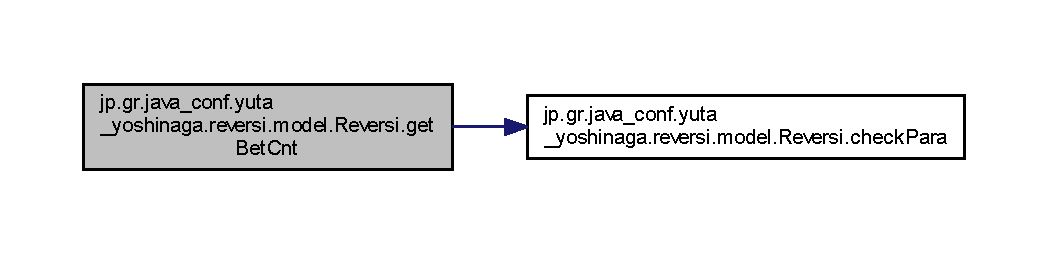
\includegraphics[width=350pt]{classjp_1_1gr_1_1java__conf_1_1yuta__yoshinaga_1_1reversi_1_1model_1_1_reversi_a9f826e110ec3298a6bc5d6987a94519c_cgraph}
\end{center}
\end{figure}
Here is the caller graph for this function\+:
\nopagebreak
\begin{figure}[H]
\begin{center}
\leavevmode
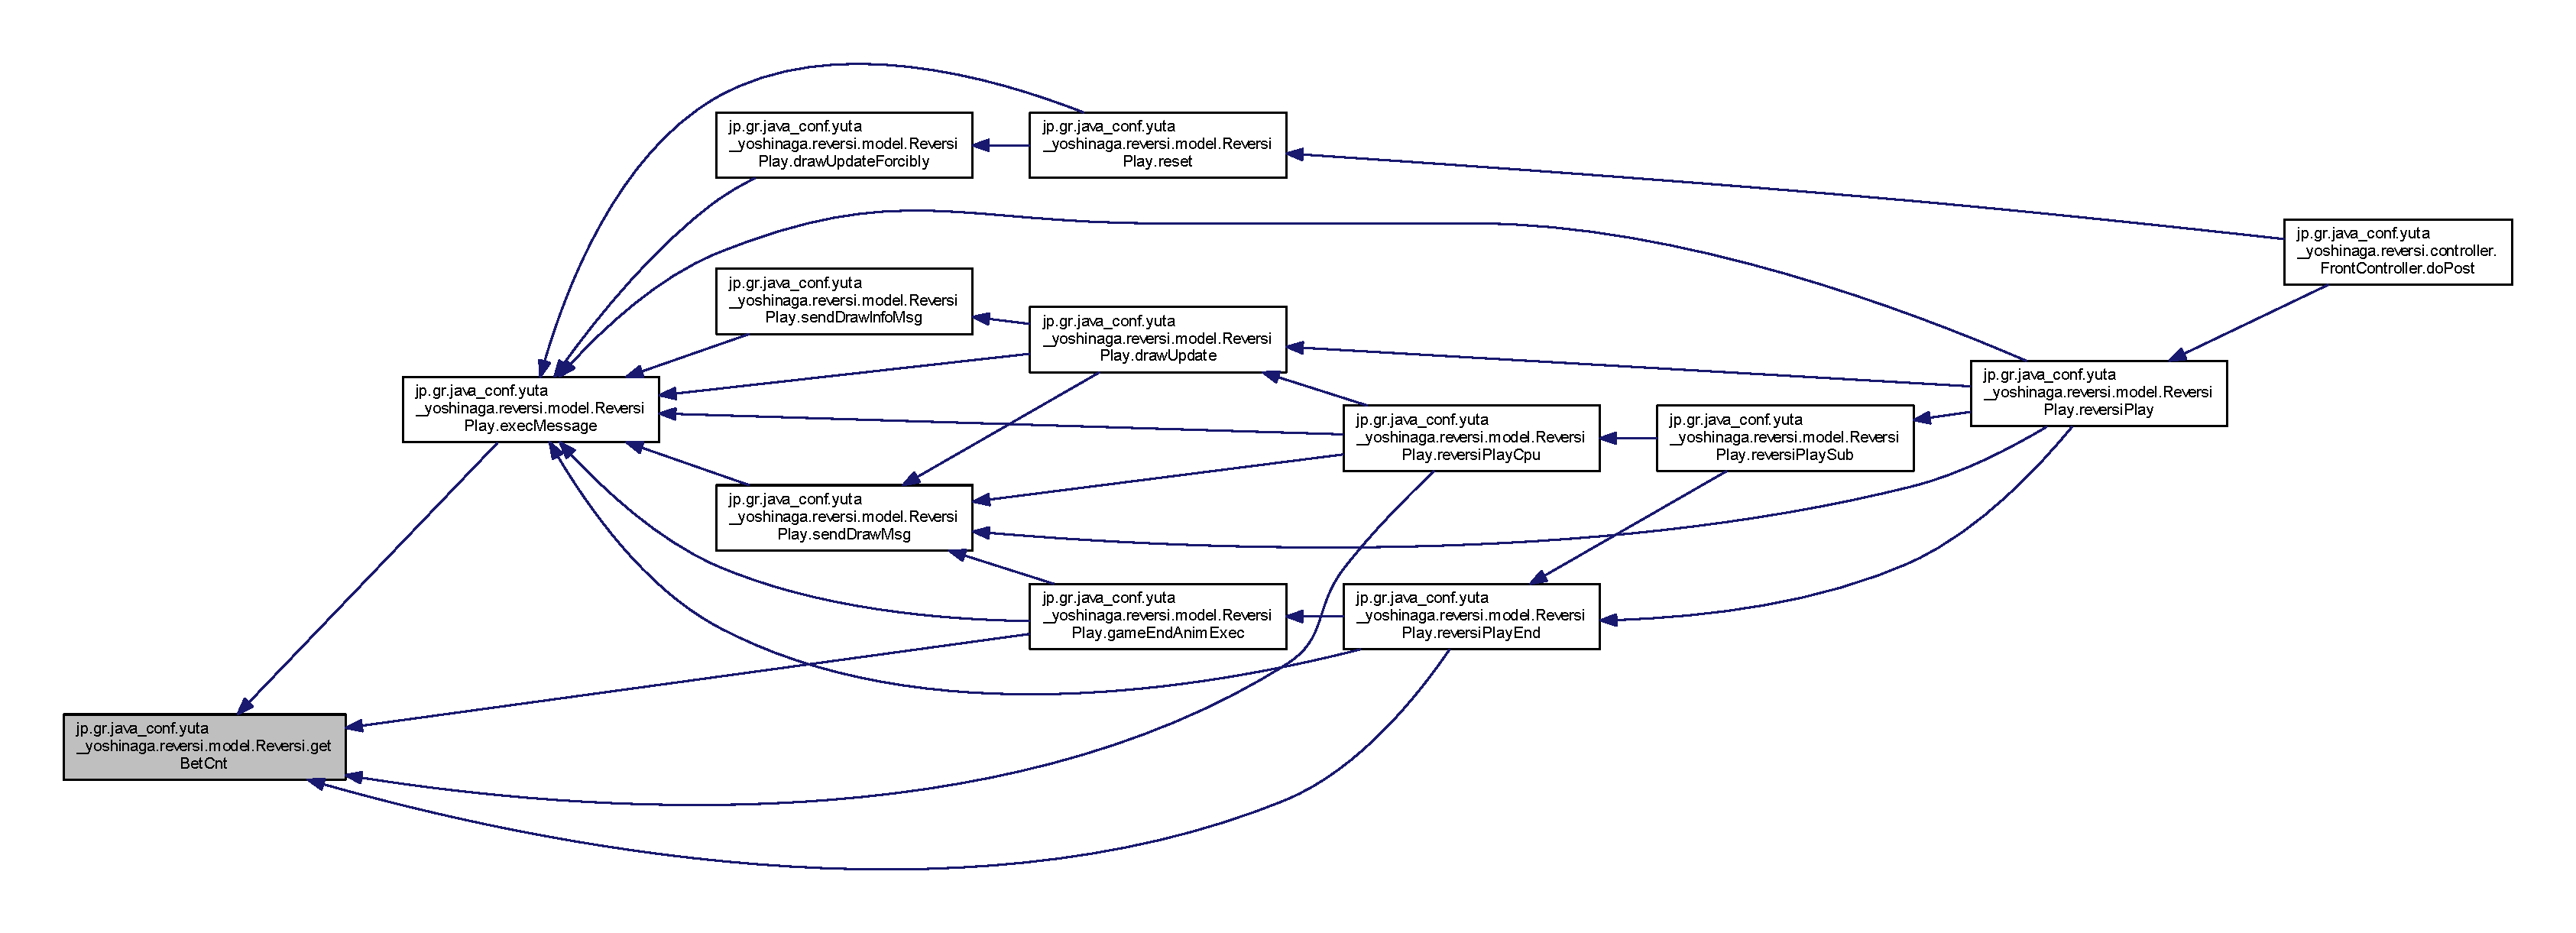
\includegraphics[width=350pt]{classjp_1_1gr_1_1java__conf_1_1yuta__yoshinaga_1_1reversi_1_1model_1_1_reversi_a9f826e110ec3298a6bc5d6987a94519c_icgraph}
\end{center}
\end{figure}
\mbox{\Hypertarget{classjp_1_1gr_1_1java__conf_1_1yuta__yoshinaga_1_1reversi_1_1model_1_1_reversi_ac6fafa41eeff56abfc67b2b5876b50f9}\label{classjp_1_1gr_1_1java__conf_1_1yuta__yoshinaga_1_1reversi_1_1model_1_1_reversi_ac6fafa41eeff56abfc67b2b5876b50f9}} 
\index{jp\+::gr\+::java\+\_\+conf\+::yuta\+\_\+yoshinaga\+::reversi\+::model\+::\+Reversi@{jp\+::gr\+::java\+\_\+conf\+::yuta\+\_\+yoshinaga\+::reversi\+::model\+::\+Reversi}!get\+Color\+Ena@{get\+Color\+Ena}}
\index{get\+Color\+Ena@{get\+Color\+Ena}!jp\+::gr\+::java\+\_\+conf\+::yuta\+\_\+yoshinaga\+::reversi\+::model\+::\+Reversi@{jp\+::gr\+::java\+\_\+conf\+::yuta\+\_\+yoshinaga\+::reversi\+::model\+::\+Reversi}}
\subsubsection{\texorpdfstring{get\+Color\+Ena()}{getColorEna()}}
{\footnotesize\ttfamily public int jp.\+gr.\+java\+\_\+conf.\+yuta\+\_\+yoshinaga.\+reversi.\+model.\+Reversi.\+get\+Color\+Ena (\begin{DoxyParamCaption}\item[{int}]{color }\end{DoxyParamCaption})}



指定色が現在置ける場所があるかチェック 


\begin{DoxyParams}[1]{Parameters}
\mbox{\tt in}  & {\em int} & color コマ色 \\
\hline
\end{DoxyParams}
\begin{DoxyReturn}{Returns}
0 \+: 成功 それ以外 \+: 失敗 
\end{DoxyReturn}
\begin{DoxyAuthor}{Author}
Yuta Yoshinaga 
\end{DoxyAuthor}
\begin{DoxyDate}{Date}
2018.\+04.\+01 
\end{DoxyDate}


Definition at line 1441 of file Reversi.\+java.



Referenced by jp.\+gr.\+java\+\_\+conf.\+yuta\+\_\+yoshinaga.\+reversi.\+model.\+Reversi.\+Analysis\+Reversi\+Black(), jp.\+gr.\+java\+\_\+conf.\+yuta\+\_\+yoshinaga.\+reversi.\+model.\+Reversi.\+Analysis\+Reversi\+White(), jp.\+gr.\+java\+\_\+conf.\+yuta\+\_\+yoshinaga.\+reversi.\+model.\+Reversi.\+get\+Game\+End\+Sts(), jp.\+gr.\+java\+\_\+conf.\+yuta\+\_\+yoshinaga.\+reversi.\+model.\+Reversi\+Play.\+reversi\+Play(), and jp.\+gr.\+java\+\_\+conf.\+yuta\+\_\+yoshinaga.\+reversi.\+model.\+Reversi\+Play.\+reversi\+Play\+Sub().

Here is the call graph for this function\+:
\nopagebreak
\begin{figure}[H]
\begin{center}
\leavevmode
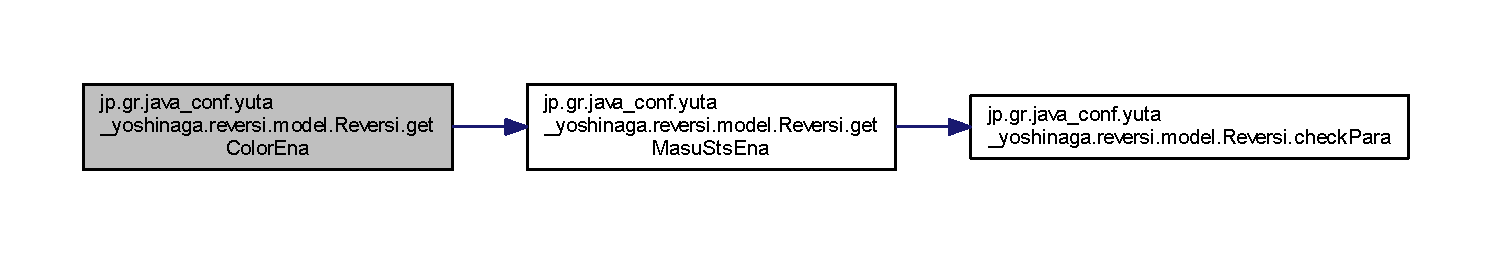
\includegraphics[width=350pt]{classjp_1_1gr_1_1java__conf_1_1yuta__yoshinaga_1_1reversi_1_1model_1_1_reversi_ac6fafa41eeff56abfc67b2b5876b50f9_cgraph}
\end{center}
\end{figure}
Here is the caller graph for this function\+:
\nopagebreak
\begin{figure}[H]
\begin{center}
\leavevmode
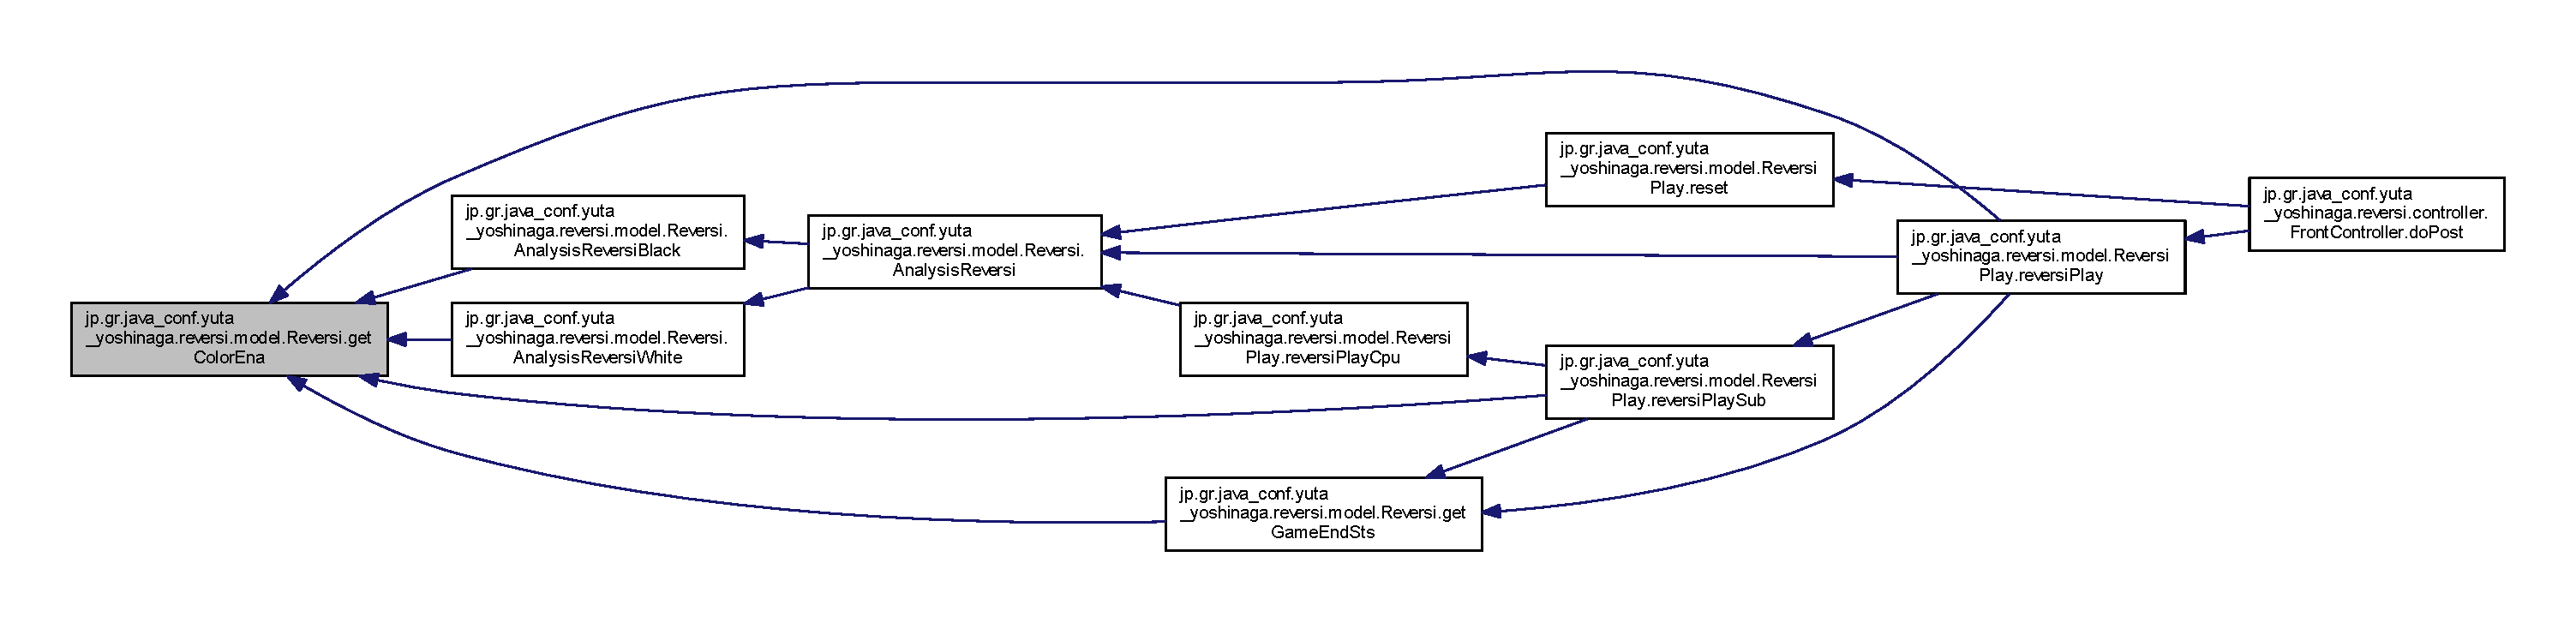
\includegraphics[width=350pt]{classjp_1_1gr_1_1java__conf_1_1yuta__yoshinaga_1_1reversi_1_1model_1_1_reversi_ac6fafa41eeff56abfc67b2b5876b50f9_icgraph}
\end{center}
\end{figure}
\mbox{\Hypertarget{classjp_1_1gr_1_1java__conf_1_1yuta__yoshinaga_1_1reversi_1_1model_1_1_reversi_aa3c701584a82e4656cb1c60123454953}\label{classjp_1_1gr_1_1java__conf_1_1yuta__yoshinaga_1_1reversi_1_1model_1_1_reversi_aa3c701584a82e4656cb1c60123454953}} 
\index{jp\+::gr\+::java\+\_\+conf\+::yuta\+\_\+yoshinaga\+::reversi\+::model\+::\+Reversi@{jp\+::gr\+::java\+\_\+conf\+::yuta\+\_\+yoshinaga\+::reversi\+::model\+::\+Reversi}!get\+Edge\+Side\+One@{get\+Edge\+Side\+One}}
\index{get\+Edge\+Side\+One@{get\+Edge\+Side\+One}!jp\+::gr\+::java\+\_\+conf\+::yuta\+\_\+yoshinaga\+::reversi\+::model\+::\+Reversi@{jp\+::gr\+::java\+\_\+conf\+::yuta\+\_\+yoshinaga\+::reversi\+::model\+::\+Reversi}}
\subsubsection{\texorpdfstring{get\+Edge\+Side\+One()}{getEdgeSideOne()}}
{\footnotesize\ttfamily public int jp.\+gr.\+java\+\_\+conf.\+yuta\+\_\+yoshinaga.\+reversi.\+model.\+Reversi.\+get\+Edge\+Side\+One (\begin{DoxyParamCaption}\item[{int}]{y,  }\item[{int}]{x }\end{DoxyParamCaption})}



指定座標が角の一つ手前か取得 


\begin{DoxyParams}[1]{Parameters}
\mbox{\tt in}  & {\em int} & y Y座標 \\
\hline
\mbox{\tt in}  & {\em int} & x X座標 \\
\hline
\end{DoxyParams}
\begin{DoxyReturn}{Returns}
0 \+: 成功 それ以外 \+: 失敗 
\end{DoxyReturn}
\begin{DoxyAuthor}{Author}
Yuta Yoshinaga 
\end{DoxyAuthor}
\begin{DoxyDate}{Date}
2018.\+04.\+01 
\end{DoxyDate}


Definition at line 1831 of file Reversi.\+java.



Referenced by jp.\+gr.\+java\+\_\+conf.\+yuta\+\_\+yoshinaga.\+reversi.\+model.\+Reversi.\+Analysis\+Reversi\+Black(), jp.\+gr.\+java\+\_\+conf.\+yuta\+\_\+yoshinaga.\+reversi.\+model.\+Reversi.\+Analysis\+Reversi\+White(), and jp.\+gr.\+java\+\_\+conf.\+yuta\+\_\+yoshinaga.\+reversi.\+model.\+Reversi\+Play.\+reversi\+Play\+Cpu().

Here is the caller graph for this function\+:
\nopagebreak
\begin{figure}[H]
\begin{center}
\leavevmode
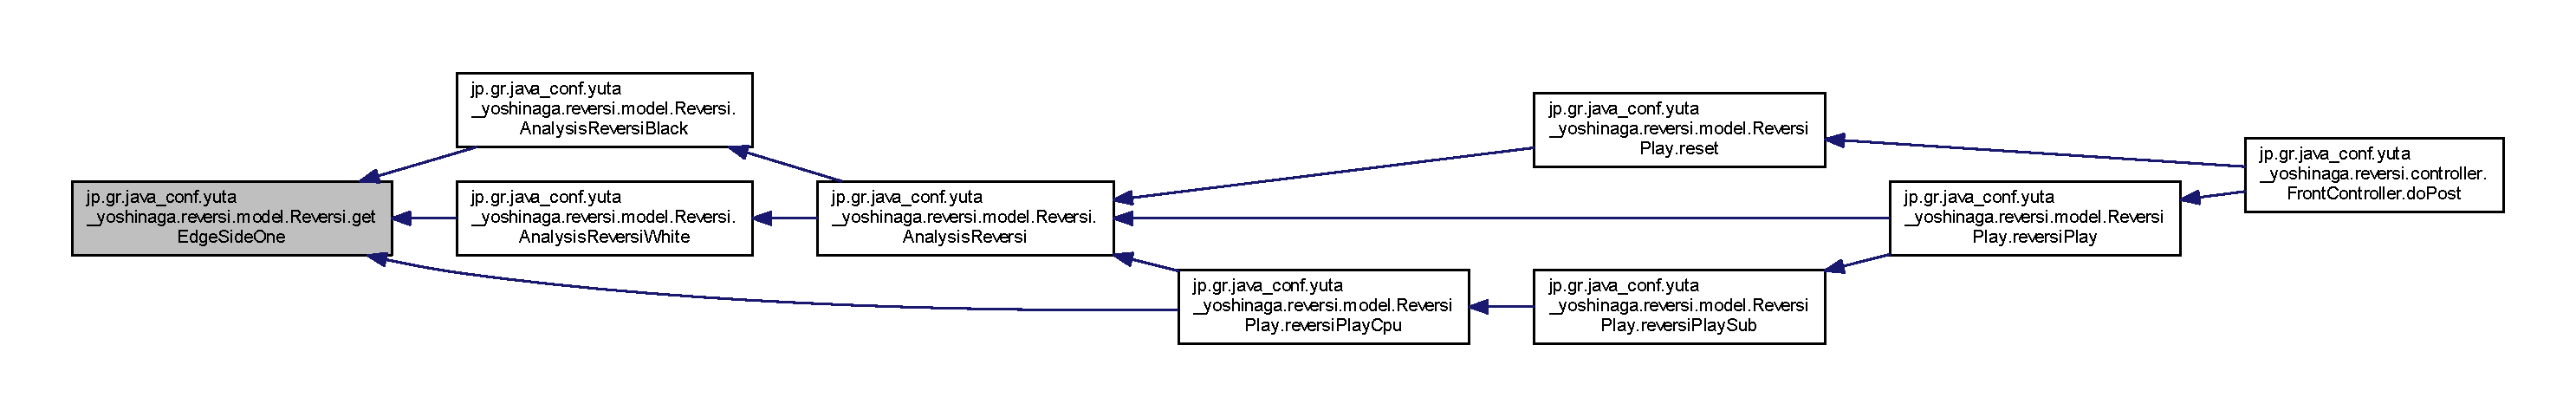
\includegraphics[width=350pt]{classjp_1_1gr_1_1java__conf_1_1yuta__yoshinaga_1_1reversi_1_1model_1_1_reversi_aa3c701584a82e4656cb1c60123454953_icgraph}
\end{center}
\end{figure}
\mbox{\Hypertarget{classjp_1_1gr_1_1java__conf_1_1yuta__yoshinaga_1_1reversi_1_1model_1_1_reversi_a296b35d2241e6b3cff31bcb199c3d9aa}\label{classjp_1_1gr_1_1java__conf_1_1yuta__yoshinaga_1_1reversi_1_1model_1_1_reversi_a296b35d2241e6b3cff31bcb199c3d9aa}} 
\index{jp\+::gr\+::java\+\_\+conf\+::yuta\+\_\+yoshinaga\+::reversi\+::model\+::\+Reversi@{jp\+::gr\+::java\+\_\+conf\+::yuta\+\_\+yoshinaga\+::reversi\+::model\+::\+Reversi}!get\+Edge\+Side\+Three@{get\+Edge\+Side\+Three}}
\index{get\+Edge\+Side\+Three@{get\+Edge\+Side\+Three}!jp\+::gr\+::java\+\_\+conf\+::yuta\+\_\+yoshinaga\+::reversi\+::model\+::\+Reversi@{jp\+::gr\+::java\+\_\+conf\+::yuta\+\_\+yoshinaga\+::reversi\+::model\+::\+Reversi}}
\subsubsection{\texorpdfstring{get\+Edge\+Side\+Three()}{getEdgeSideThree()}}
{\footnotesize\ttfamily public int jp.\+gr.\+java\+\_\+conf.\+yuta\+\_\+yoshinaga.\+reversi.\+model.\+Reversi.\+get\+Edge\+Side\+Three (\begin{DoxyParamCaption}\item[{int}]{y,  }\item[{int}]{x }\end{DoxyParamCaption})}



指定座標が角の三つ以上手前か取得 


\begin{DoxyParams}[1]{Parameters}
\mbox{\tt in}  & {\em int} & y Y座標 \\
\hline
\mbox{\tt in}  & {\em int} & x X座標 \\
\hline
\end{DoxyParams}
\begin{DoxyReturn}{Returns}
0 \+: 成功 それ以外 \+: 失敗 
\end{DoxyReturn}
\begin{DoxyAuthor}{Author}
Yuta Yoshinaga 
\end{DoxyAuthor}
\begin{DoxyDate}{Date}
2018.\+04.\+01 
\end{DoxyDate}


Definition at line 1895 of file Reversi.\+java.



Referenced by jp.\+gr.\+java\+\_\+conf.\+yuta\+\_\+yoshinaga.\+reversi.\+model.\+Reversi.\+Analysis\+Reversi\+Black(), jp.\+gr.\+java\+\_\+conf.\+yuta\+\_\+yoshinaga.\+reversi.\+model.\+Reversi.\+Analysis\+Reversi\+White(), and jp.\+gr.\+java\+\_\+conf.\+yuta\+\_\+yoshinaga.\+reversi.\+model.\+Reversi\+Play.\+reversi\+Play\+Cpu().

Here is the caller graph for this function\+:
\nopagebreak
\begin{figure}[H]
\begin{center}
\leavevmode
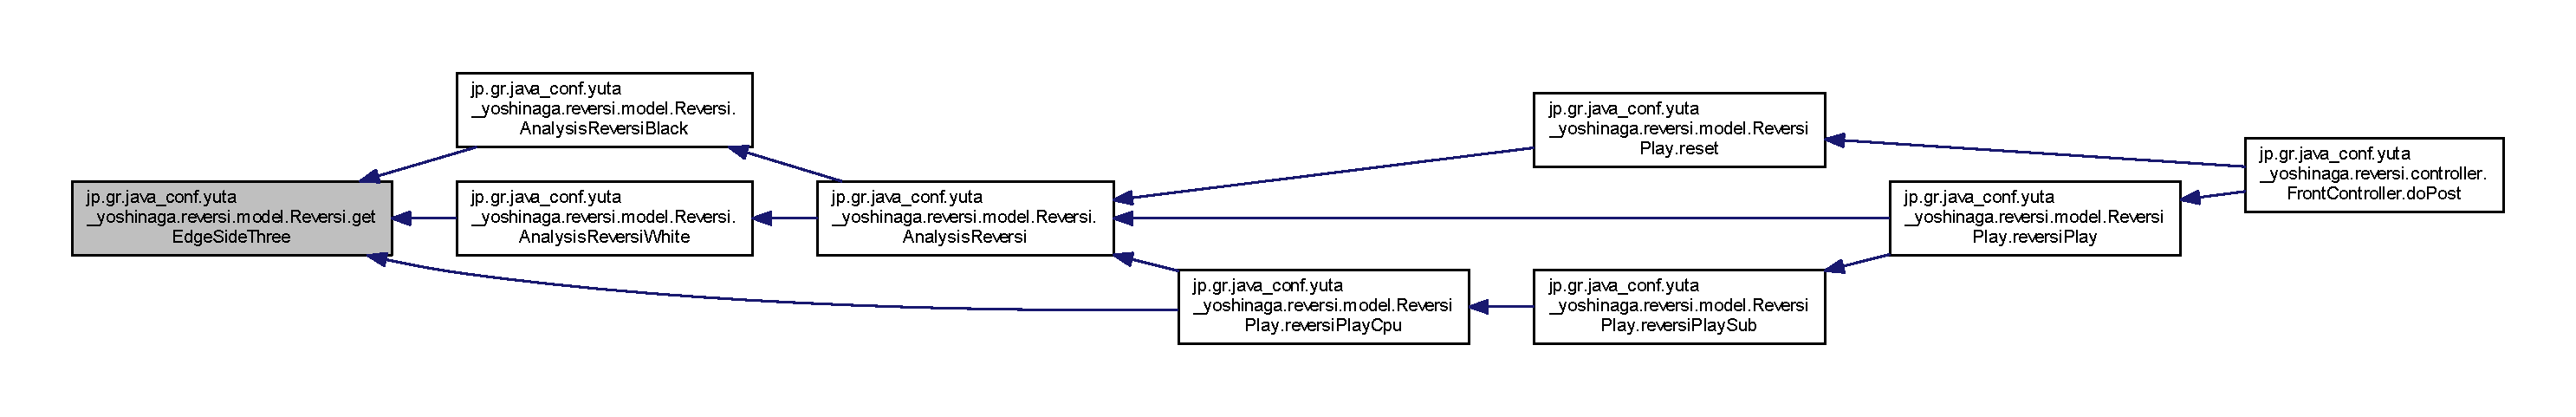
\includegraphics[width=350pt]{classjp_1_1gr_1_1java__conf_1_1yuta__yoshinaga_1_1reversi_1_1model_1_1_reversi_a296b35d2241e6b3cff31bcb199c3d9aa_icgraph}
\end{center}
\end{figure}
\mbox{\Hypertarget{classjp_1_1gr_1_1java__conf_1_1yuta__yoshinaga_1_1reversi_1_1model_1_1_reversi_afc0b642f56e39a28ab5adc48c8fd2b98}\label{classjp_1_1gr_1_1java__conf_1_1yuta__yoshinaga_1_1reversi_1_1model_1_1_reversi_afc0b642f56e39a28ab5adc48c8fd2b98}} 
\index{jp\+::gr\+::java\+\_\+conf\+::yuta\+\_\+yoshinaga\+::reversi\+::model\+::\+Reversi@{jp\+::gr\+::java\+\_\+conf\+::yuta\+\_\+yoshinaga\+::reversi\+::model\+::\+Reversi}!get\+Edge\+Side\+Two@{get\+Edge\+Side\+Two}}
\index{get\+Edge\+Side\+Two@{get\+Edge\+Side\+Two}!jp\+::gr\+::java\+\_\+conf\+::yuta\+\_\+yoshinaga\+::reversi\+::model\+::\+Reversi@{jp\+::gr\+::java\+\_\+conf\+::yuta\+\_\+yoshinaga\+::reversi\+::model\+::\+Reversi}}
\subsubsection{\texorpdfstring{get\+Edge\+Side\+Two()}{getEdgeSideTwo()}}
{\footnotesize\ttfamily public int jp.\+gr.\+java\+\_\+conf.\+yuta\+\_\+yoshinaga.\+reversi.\+model.\+Reversi.\+get\+Edge\+Side\+Two (\begin{DoxyParamCaption}\item[{int}]{y,  }\item[{int}]{x }\end{DoxyParamCaption})}



指定座標が角の二つ手前か取得 


\begin{DoxyParams}[1]{Parameters}
\mbox{\tt in}  & {\em int} & y Y座標 \\
\hline
\mbox{\tt in}  & {\em int} & x X座標 \\
\hline
\end{DoxyParams}
\begin{DoxyReturn}{Returns}
0 \+: 成功 それ以外 \+: 失敗 
\end{DoxyReturn}
\begin{DoxyAuthor}{Author}
Yuta Yoshinaga 
\end{DoxyAuthor}
\begin{DoxyDate}{Date}
2018.\+04.\+01 
\end{DoxyDate}


Definition at line 1863 of file Reversi.\+java.



Referenced by jp.\+gr.\+java\+\_\+conf.\+yuta\+\_\+yoshinaga.\+reversi.\+model.\+Reversi.\+Analysis\+Reversi\+Black(), jp.\+gr.\+java\+\_\+conf.\+yuta\+\_\+yoshinaga.\+reversi.\+model.\+Reversi.\+Analysis\+Reversi\+White(), and jp.\+gr.\+java\+\_\+conf.\+yuta\+\_\+yoshinaga.\+reversi.\+model.\+Reversi\+Play.\+reversi\+Play\+Cpu().

Here is the caller graph for this function\+:
\nopagebreak
\begin{figure}[H]
\begin{center}
\leavevmode
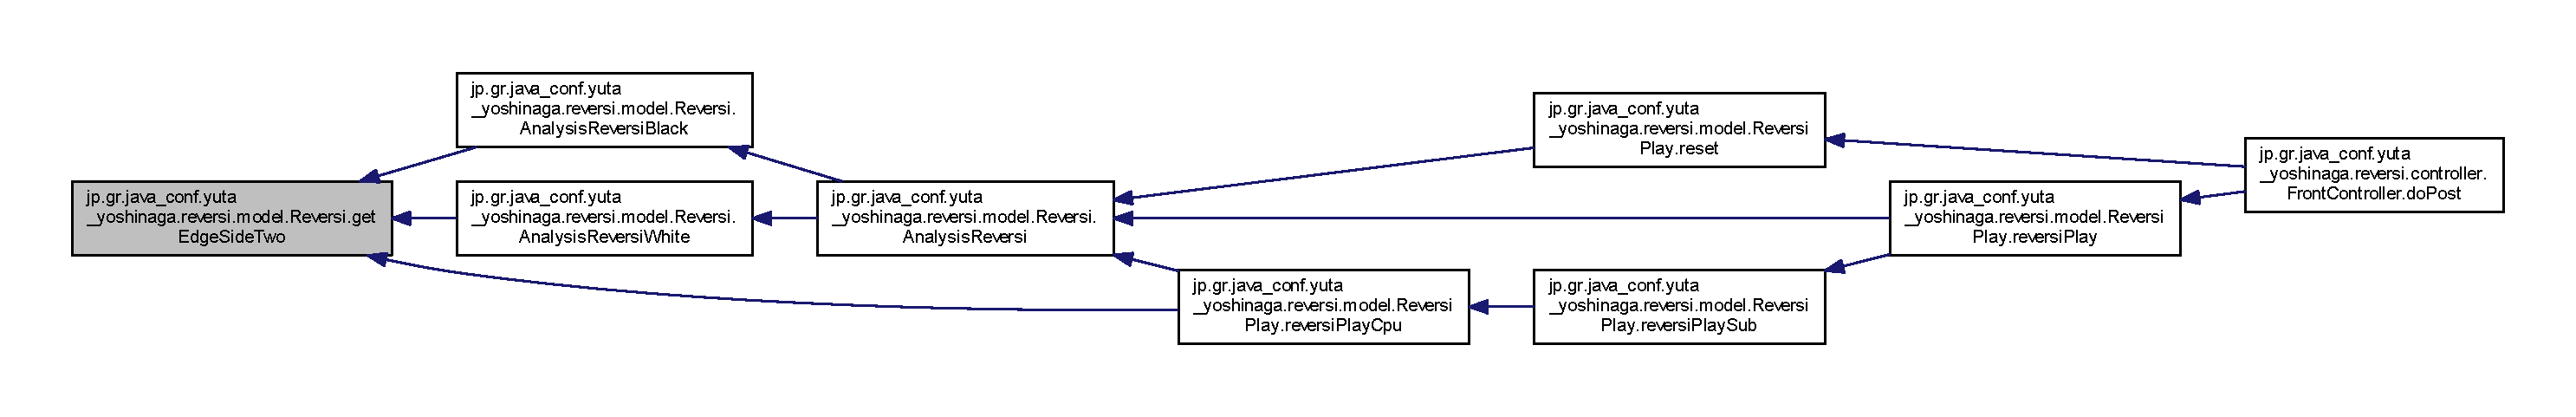
\includegraphics[width=350pt]{classjp_1_1gr_1_1java__conf_1_1yuta__yoshinaga_1_1reversi_1_1model_1_1_reversi_afc0b642f56e39a28ab5adc48c8fd2b98_icgraph}
\end{center}
\end{figure}
\mbox{\Hypertarget{classjp_1_1gr_1_1java__conf_1_1yuta__yoshinaga_1_1reversi_1_1model_1_1_reversi_a3989b051544745724fc372d4a6b8a7f7}\label{classjp_1_1gr_1_1java__conf_1_1yuta__yoshinaga_1_1reversi_1_1model_1_1_reversi_a3989b051544745724fc372d4a6b8a7f7}} 
\index{jp\+::gr\+::java\+\_\+conf\+::yuta\+\_\+yoshinaga\+::reversi\+::model\+::\+Reversi@{jp\+::gr\+::java\+\_\+conf\+::yuta\+\_\+yoshinaga\+::reversi\+::model\+::\+Reversi}!get\+Edge\+Side\+Zero@{get\+Edge\+Side\+Zero}}
\index{get\+Edge\+Side\+Zero@{get\+Edge\+Side\+Zero}!jp\+::gr\+::java\+\_\+conf\+::yuta\+\_\+yoshinaga\+::reversi\+::model\+::\+Reversi@{jp\+::gr\+::java\+\_\+conf\+::yuta\+\_\+yoshinaga\+::reversi\+::model\+::\+Reversi}}
\subsubsection{\texorpdfstring{get\+Edge\+Side\+Zero()}{getEdgeSideZero()}}
{\footnotesize\ttfamily public int jp.\+gr.\+java\+\_\+conf.\+yuta\+\_\+yoshinaga.\+reversi.\+model.\+Reversi.\+get\+Edge\+Side\+Zero (\begin{DoxyParamCaption}\item[{int}]{y,  }\item[{int}]{x }\end{DoxyParamCaption})}



指定座標が角か取得 


\begin{DoxyParams}[1]{Parameters}
\mbox{\tt in}  & {\em int} & y Y座標 \\
\hline
\mbox{\tt in}  & {\em int} & x X座標 \\
\hline
\end{DoxyParams}
\begin{DoxyReturn}{Returns}
0 \+: 成功 それ以外 \+: 失敗 
\end{DoxyReturn}
\begin{DoxyAuthor}{Author}
Yuta Yoshinaga 
\end{DoxyAuthor}
\begin{DoxyDate}{Date}
2018.\+04.\+01 
\end{DoxyDate}


Definition at line 1807 of file Reversi.\+java.



Referenced by jp.\+gr.\+java\+\_\+conf.\+yuta\+\_\+yoshinaga.\+reversi.\+model.\+Reversi.\+Analysis\+Reversi\+Black(), jp.\+gr.\+java\+\_\+conf.\+yuta\+\_\+yoshinaga.\+reversi.\+model.\+Reversi.\+Analysis\+Reversi\+White(), and jp.\+gr.\+java\+\_\+conf.\+yuta\+\_\+yoshinaga.\+reversi.\+model.\+Reversi\+Play.\+reversi\+Play\+Cpu().

Here is the caller graph for this function\+:
\nopagebreak
\begin{figure}[H]
\begin{center}
\leavevmode
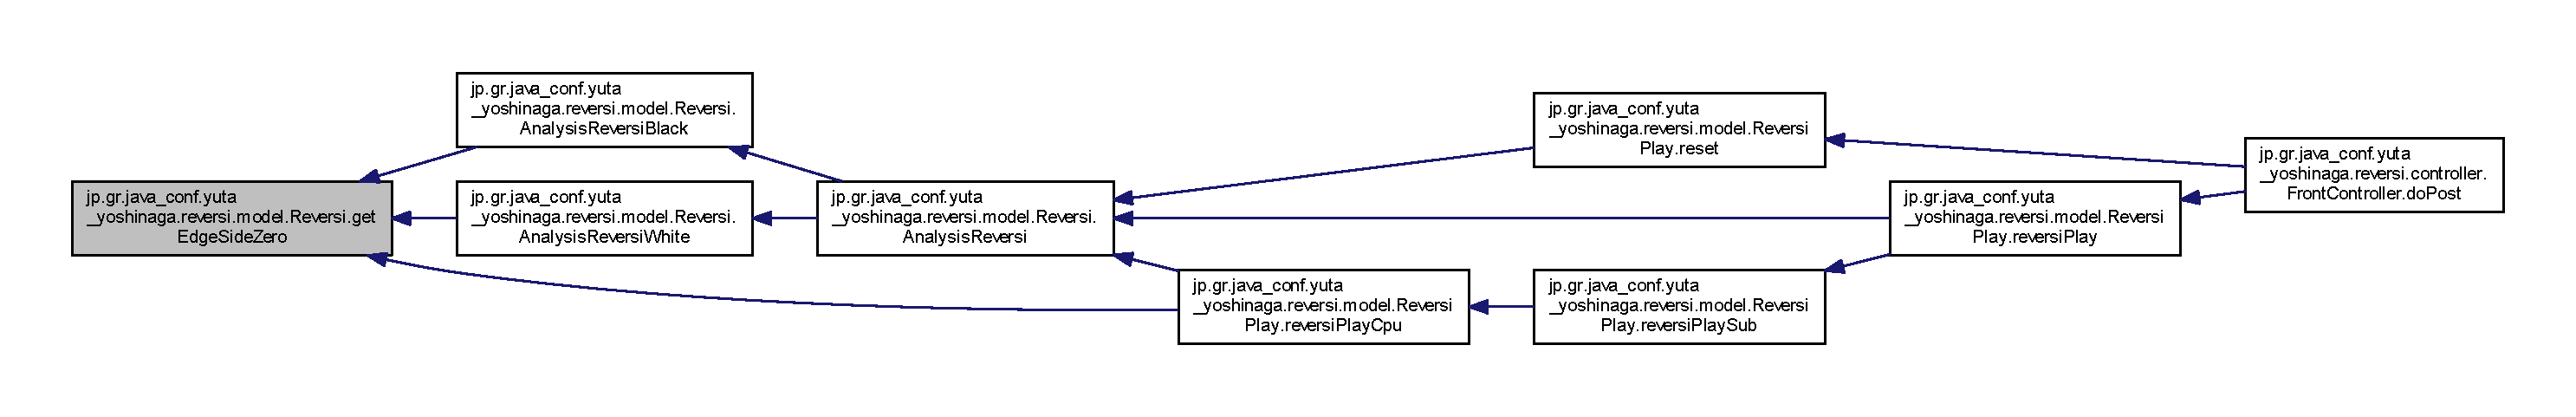
\includegraphics[width=350pt]{classjp_1_1gr_1_1java__conf_1_1yuta__yoshinaga_1_1reversi_1_1model_1_1_reversi_a3989b051544745724fc372d4a6b8a7f7_icgraph}
\end{center}
\end{figure}
\mbox{\Hypertarget{classjp_1_1gr_1_1java__conf_1_1yuta__yoshinaga_1_1reversi_1_1model_1_1_reversi_abc97a3ba932ee271cf04ff0f72162100}\label{classjp_1_1gr_1_1java__conf_1_1yuta__yoshinaga_1_1reversi_1_1model_1_1_reversi_abc97a3ba932ee271cf04ff0f72162100}} 
\index{jp\+::gr\+::java\+\_\+conf\+::yuta\+\_\+yoshinaga\+::reversi\+::model\+::\+Reversi@{jp\+::gr\+::java\+\_\+conf\+::yuta\+\_\+yoshinaga\+::reversi\+::model\+::\+Reversi}!get\+Game\+End\+Sts@{get\+Game\+End\+Sts}}
\index{get\+Game\+End\+Sts@{get\+Game\+End\+Sts}!jp\+::gr\+::java\+\_\+conf\+::yuta\+\_\+yoshinaga\+::reversi\+::model\+::\+Reversi@{jp\+::gr\+::java\+\_\+conf\+::yuta\+\_\+yoshinaga\+::reversi\+::model\+::\+Reversi}}
\subsubsection{\texorpdfstring{get\+Game\+End\+Sts()}{getGameEndSts()}}
{\footnotesize\ttfamily public int jp.\+gr.\+java\+\_\+conf.\+yuta\+\_\+yoshinaga.\+reversi.\+model.\+Reversi.\+get\+Game\+End\+Sts (\begin{DoxyParamCaption}{ }\end{DoxyParamCaption})}



ゲーム終了かチェック 

\begin{DoxyReturn}{Returns}
0 \+: 続行 それ以外 \+: ゲーム終了 
\end{DoxyReturn}
\begin{DoxyAuthor}{Author}
Yuta Yoshinaga 
\end{DoxyAuthor}
\begin{DoxyDate}{Date}
2018.\+04.\+01 
\end{DoxyDate}


Definition at line 1463 of file Reversi.\+java.



Referenced by jp.\+gr.\+java\+\_\+conf.\+yuta\+\_\+yoshinaga.\+reversi.\+model.\+Reversi\+Play.\+reversi\+Play(), and jp.\+gr.\+java\+\_\+conf.\+yuta\+\_\+yoshinaga.\+reversi.\+model.\+Reversi\+Play.\+reversi\+Play\+Sub().

Here is the call graph for this function\+:
\nopagebreak
\begin{figure}[H]
\begin{center}
\leavevmode
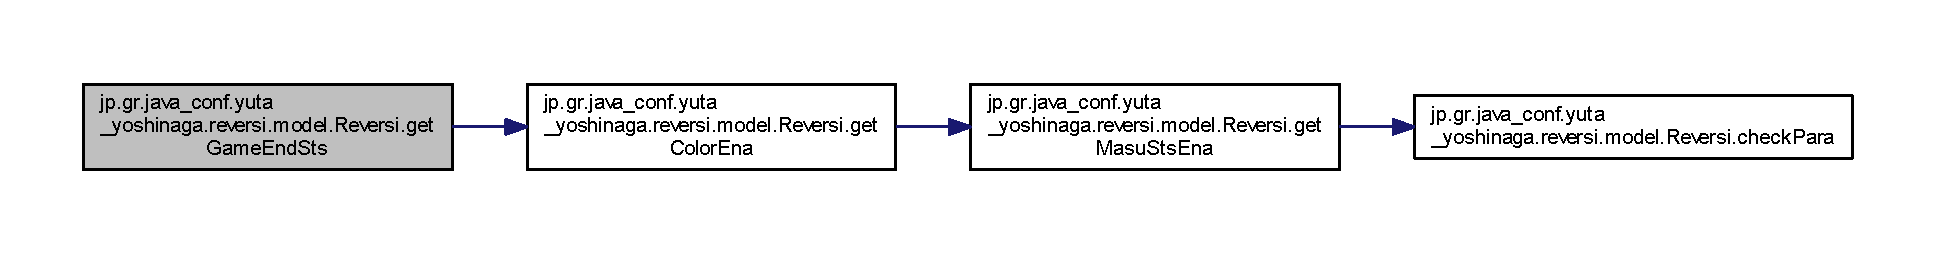
\includegraphics[width=350pt]{classjp_1_1gr_1_1java__conf_1_1yuta__yoshinaga_1_1reversi_1_1model_1_1_reversi_abc97a3ba932ee271cf04ff0f72162100_cgraph}
\end{center}
\end{figure}
Here is the caller graph for this function\+:
\nopagebreak
\begin{figure}[H]
\begin{center}
\leavevmode
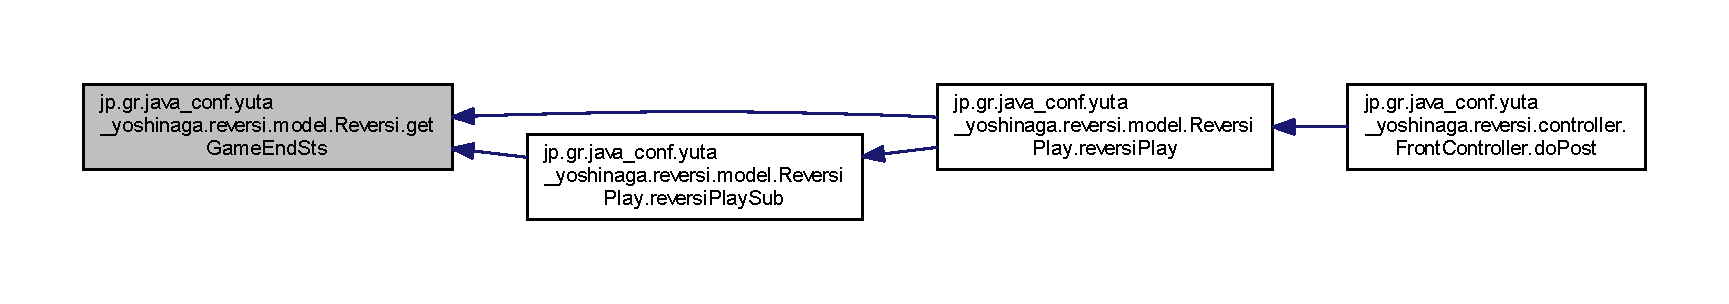
\includegraphics[width=350pt]{classjp_1_1gr_1_1java__conf_1_1yuta__yoshinaga_1_1reversi_1_1model_1_1_reversi_abc97a3ba932ee271cf04ff0f72162100_icgraph}
\end{center}
\end{figure}
\mbox{\Hypertarget{classjp_1_1gr_1_1java__conf_1_1yuta__yoshinaga_1_1reversi_1_1model_1_1_reversi_af781f5ebb4fb33b574ec58acfb45a796}\label{classjp_1_1gr_1_1java__conf_1_1yuta__yoshinaga_1_1reversi_1_1model_1_1_reversi_af781f5ebb4fb33b574ec58acfb45a796}} 
\index{jp\+::gr\+::java\+\_\+conf\+::yuta\+\_\+yoshinaga\+::reversi\+::model\+::\+Reversi@{jp\+::gr\+::java\+\_\+conf\+::yuta\+\_\+yoshinaga\+::reversi\+::model\+::\+Reversi}!get\+History@{get\+History}}
\index{get\+History@{get\+History}!jp\+::gr\+::java\+\_\+conf\+::yuta\+\_\+yoshinaga\+::reversi\+::model\+::\+Reversi@{jp\+::gr\+::java\+\_\+conf\+::yuta\+\_\+yoshinaga\+::reversi\+::model\+::\+Reversi}}
\subsubsection{\texorpdfstring{get\+History()}{getHistory()}}
{\footnotesize\ttfamily public \hyperlink{classjp_1_1gr_1_1java__conf_1_1yuta__yoshinaga_1_1reversi_1_1model_1_1_reversi_history}{Reversi\+History} jp.\+gr.\+java\+\_\+conf.\+yuta\+\_\+yoshinaga.\+reversi.\+model.\+Reversi.\+get\+History (\begin{DoxyParamCaption}\item[{int}]{num }\end{DoxyParamCaption})}



履歴取得 


\begin{DoxyParams}[1]{Parameters}
\mbox{\tt in}  & {\em int} & num ポイント \\
\hline
\end{DoxyParams}
\begin{DoxyReturn}{Returns}
履歴 null \+: 失敗 
\end{DoxyReturn}
\begin{DoxyAuthor}{Author}
Yuta Yoshinaga 
\end{DoxyAuthor}
\begin{DoxyDate}{Date}
2018.\+04.\+01 
\end{DoxyDate}


Definition at line 1637 of file Reversi.\+java.

Here is the call graph for this function\+:
\nopagebreak
\begin{figure}[H]
\begin{center}
\leavevmode
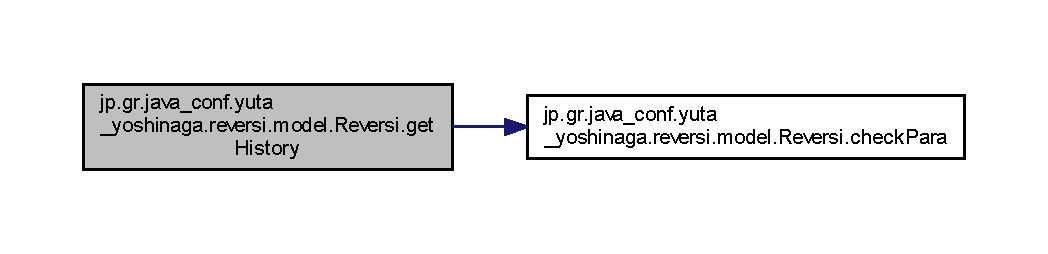
\includegraphics[width=350pt]{classjp_1_1gr_1_1java__conf_1_1yuta__yoshinaga_1_1reversi_1_1model_1_1_reversi_af781f5ebb4fb33b574ec58acfb45a796_cgraph}
\end{center}
\end{figure}
\mbox{\Hypertarget{classjp_1_1gr_1_1java__conf_1_1yuta__yoshinaga_1_1reversi_1_1model_1_1_reversi_a286949e070d0cfc8a1d9562a298b7b98}\label{classjp_1_1gr_1_1java__conf_1_1yuta__yoshinaga_1_1reversi_1_1model_1_1_reversi_a286949e070d0cfc8a1d9562a298b7b98}} 
\index{jp\+::gr\+::java\+\_\+conf\+::yuta\+\_\+yoshinaga\+::reversi\+::model\+::\+Reversi@{jp\+::gr\+::java\+\_\+conf\+::yuta\+\_\+yoshinaga\+::reversi\+::model\+::\+Reversi}!get\+History\+Cnt@{get\+History\+Cnt}}
\index{get\+History\+Cnt@{get\+History\+Cnt}!jp\+::gr\+::java\+\_\+conf\+::yuta\+\_\+yoshinaga\+::reversi\+::model\+::\+Reversi@{jp\+::gr\+::java\+\_\+conf\+::yuta\+\_\+yoshinaga\+::reversi\+::model\+::\+Reversi}}
\subsubsection{\texorpdfstring{get\+History\+Cnt()}{getHistoryCnt()}}
{\footnotesize\ttfamily public int jp.\+gr.\+java\+\_\+conf.\+yuta\+\_\+yoshinaga.\+reversi.\+model.\+Reversi.\+get\+History\+Cnt (\begin{DoxyParamCaption}{ }\end{DoxyParamCaption})}



履歴数取得 

\begin{DoxyReturn}{Returns}
履歴数 
\end{DoxyReturn}
\begin{DoxyAuthor}{Author}
Yuta Yoshinaga 
\end{DoxyAuthor}
\begin{DoxyDate}{Date}
2018.\+04.\+01 
\end{DoxyDate}


Definition at line 1654 of file Reversi.\+java.

\mbox{\Hypertarget{classjp_1_1gr_1_1java__conf_1_1yuta__yoshinaga_1_1reversi_1_1model_1_1_reversi_aaab64f3b70ed5da5f0707933cbf82802}\label{classjp_1_1gr_1_1java__conf_1_1yuta__yoshinaga_1_1reversi_1_1model_1_1_reversi_aaab64f3b70ed5da5f0707933cbf82802}} 
\index{jp\+::gr\+::java\+\_\+conf\+::yuta\+\_\+yoshinaga\+::reversi\+::model\+::\+Reversi@{jp\+::gr\+::java\+\_\+conf\+::yuta\+\_\+yoshinaga\+::reversi\+::model\+::\+Reversi}!get\+Masu\+Sts@{get\+Masu\+Sts}}
\index{get\+Masu\+Sts@{get\+Masu\+Sts}!jp\+::gr\+::java\+\_\+conf\+::yuta\+\_\+yoshinaga\+::reversi\+::model\+::\+Reversi@{jp\+::gr\+::java\+\_\+conf\+::yuta\+\_\+yoshinaga\+::reversi\+::model\+::\+Reversi}}
\subsubsection{\texorpdfstring{get\+Masu\+Sts()}{getMasuSts()}}
{\footnotesize\ttfamily public int jp.\+gr.\+java\+\_\+conf.\+yuta\+\_\+yoshinaga.\+reversi.\+model.\+Reversi.\+get\+Masu\+Sts (\begin{DoxyParamCaption}\item[{int}]{y,  }\item[{int}]{x }\end{DoxyParamCaption})}



マスステータスを取得 


\begin{DoxyParams}[1]{Parameters}
\mbox{\tt in}  & {\em int} & y 取得するマスの\+Y座標 \\
\hline
\mbox{\tt in}  & {\em int} & x 取得するマスの\+X座標 \\
\hline
\end{DoxyParams}
\begin{DoxyReturn}{Returns}
-\/1 \+: 失敗 それ以外 \+: マスステータス 
\end{DoxyReturn}
\begin{DoxyAuthor}{Author}
Yuta Yoshinaga 
\end{DoxyAuthor}
\begin{DoxyDate}{Date}
2018.\+04.\+01 
\end{DoxyDate}


Definition at line 1366 of file Reversi.\+java.



Referenced by jp.\+gr.\+java\+\_\+conf.\+yuta\+\_\+yoshinaga.\+reversi.\+model.\+Reversi.\+check\+Edge(), jp.\+gr.\+java\+\_\+conf.\+yuta\+\_\+yoshinaga.\+reversi.\+model.\+Reversi\+Play.\+draw\+Update(), and jp.\+gr.\+java\+\_\+conf.\+yuta\+\_\+yoshinaga.\+reversi.\+model.\+Reversi\+Play.\+exec\+Message().

Here is the call graph for this function\+:
\nopagebreak
\begin{figure}[H]
\begin{center}
\leavevmode
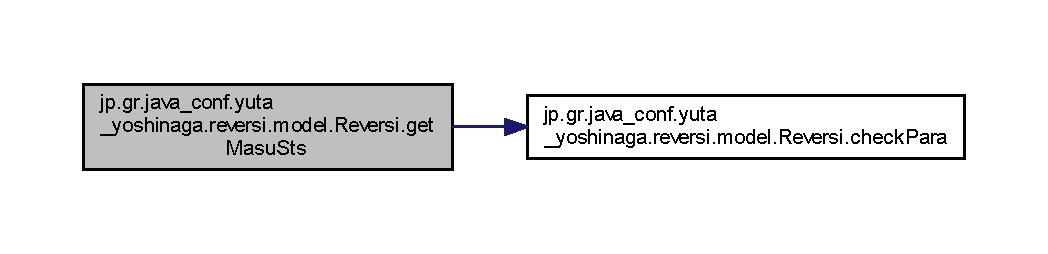
\includegraphics[width=350pt]{classjp_1_1gr_1_1java__conf_1_1yuta__yoshinaga_1_1reversi_1_1model_1_1_reversi_aaab64f3b70ed5da5f0707933cbf82802_cgraph}
\end{center}
\end{figure}
Here is the caller graph for this function\+:
\nopagebreak
\begin{figure}[H]
\begin{center}
\leavevmode
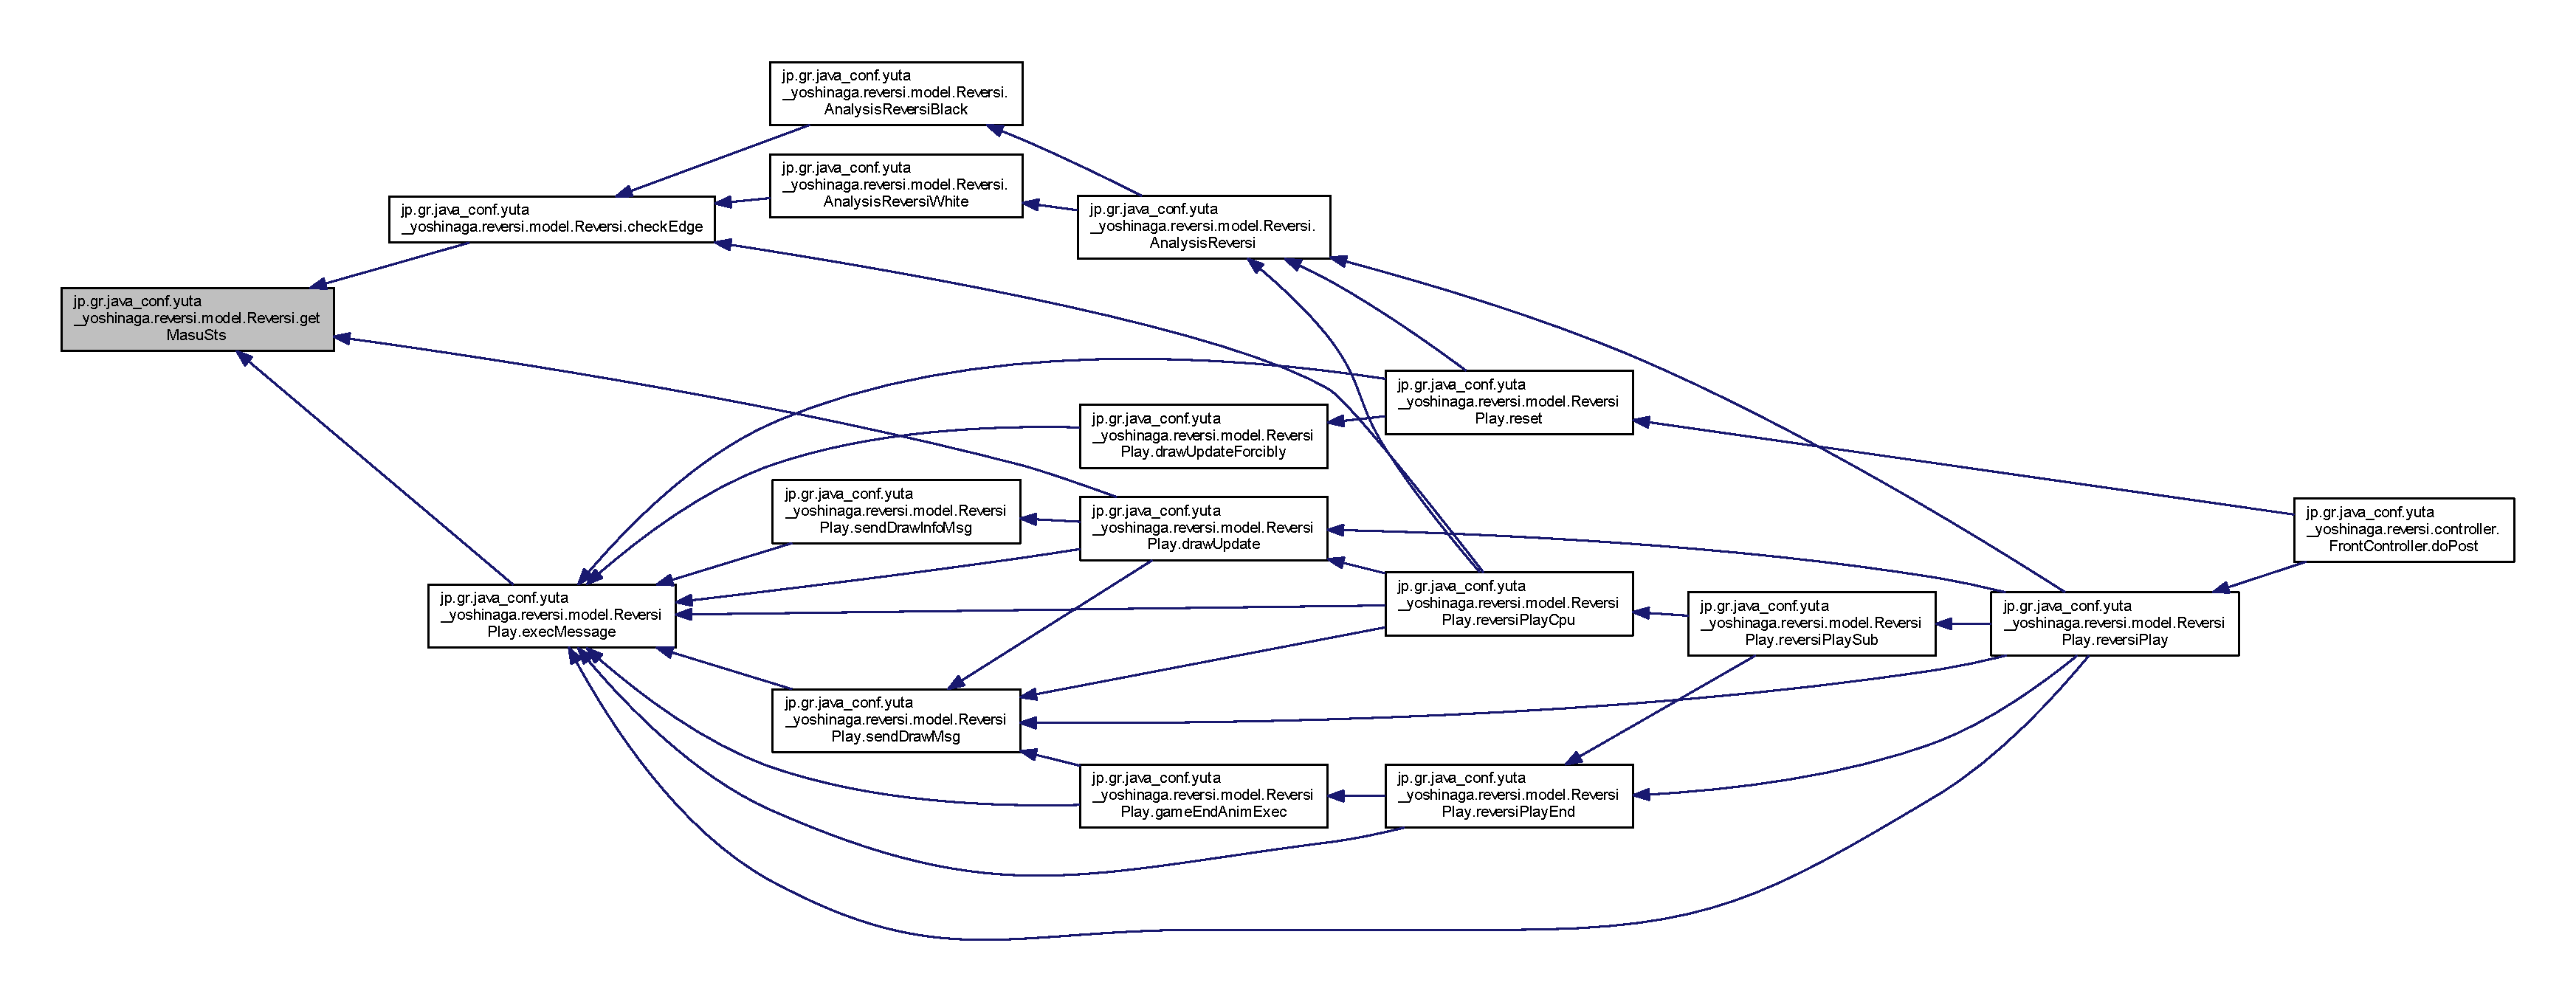
\includegraphics[width=350pt]{classjp_1_1gr_1_1java__conf_1_1yuta__yoshinaga_1_1reversi_1_1model_1_1_reversi_aaab64f3b70ed5da5f0707933cbf82802_icgraph}
\end{center}
\end{figure}
\mbox{\Hypertarget{classjp_1_1gr_1_1java__conf_1_1yuta__yoshinaga_1_1reversi_1_1model_1_1_reversi_a1a528710342faba65975f4768d24b129}\label{classjp_1_1gr_1_1java__conf_1_1yuta__yoshinaga_1_1reversi_1_1model_1_1_reversi_a1a528710342faba65975f4768d24b129}} 
\index{jp\+::gr\+::java\+\_\+conf\+::yuta\+\_\+yoshinaga\+::reversi\+::model\+::\+Reversi@{jp\+::gr\+::java\+\_\+conf\+::yuta\+\_\+yoshinaga\+::reversi\+::model\+::\+Reversi}!get\+Masu\+Sts\+Cnt@{get\+Masu\+Sts\+Cnt}}
\index{get\+Masu\+Sts\+Cnt@{get\+Masu\+Sts\+Cnt}!jp\+::gr\+::java\+\_\+conf\+::yuta\+\_\+yoshinaga\+::reversi\+::model\+::\+Reversi@{jp\+::gr\+::java\+\_\+conf\+::yuta\+\_\+yoshinaga\+::reversi\+::model\+::\+Reversi}}
\subsubsection{\texorpdfstring{get\+Masu\+Sts\+Cnt()}{getMasuStsCnt()}}
{\footnotesize\ttfamily public int jp.\+gr.\+java\+\_\+conf.\+yuta\+\_\+yoshinaga.\+reversi.\+model.\+Reversi.\+get\+Masu\+Sts\+Cnt (\begin{DoxyParamCaption}\item[{int}]{color,  }\item[{int}]{y,  }\item[{int}]{x }\end{DoxyParamCaption})}



指定座標の獲得コマ数取得 


\begin{DoxyParams}[1]{Parameters}
\mbox{\tt in}  & {\em int} & color コマ色 \\
\hline
\mbox{\tt in}  & {\em int} & y マスの\+Y座標 \\
\hline
\mbox{\tt in}  & {\em int} & x マスの\+X座標 \\
\hline
\end{DoxyParams}
\begin{DoxyReturn}{Returns}
-\/1 \+: 失敗 それ以外 \+: 獲得コマ数 
\end{DoxyReturn}
\begin{DoxyAuthor}{Author}
Yuta Yoshinaga 
\end{DoxyAuthor}
\begin{DoxyDate}{Date}
2018.\+04.\+01 
\end{DoxyDate}


Definition at line 1422 of file Reversi.\+java.



Referenced by jp.\+gr.\+java\+\_\+conf.\+yuta\+\_\+yoshinaga.\+reversi.\+model.\+Reversi\+Play.\+exec\+Message(), and jp.\+gr.\+java\+\_\+conf.\+yuta\+\_\+yoshinaga.\+reversi.\+model.\+Reversi\+Play.\+reversi\+Play\+Cpu().

Here is the call graph for this function\+:
\nopagebreak
\begin{figure}[H]
\begin{center}
\leavevmode
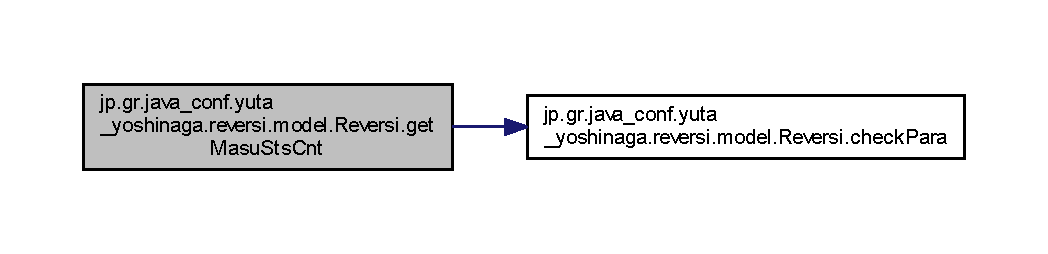
\includegraphics[width=350pt]{classjp_1_1gr_1_1java__conf_1_1yuta__yoshinaga_1_1reversi_1_1model_1_1_reversi_a1a528710342faba65975f4768d24b129_cgraph}
\end{center}
\end{figure}
Here is the caller graph for this function\+:
\nopagebreak
\begin{figure}[H]
\begin{center}
\leavevmode
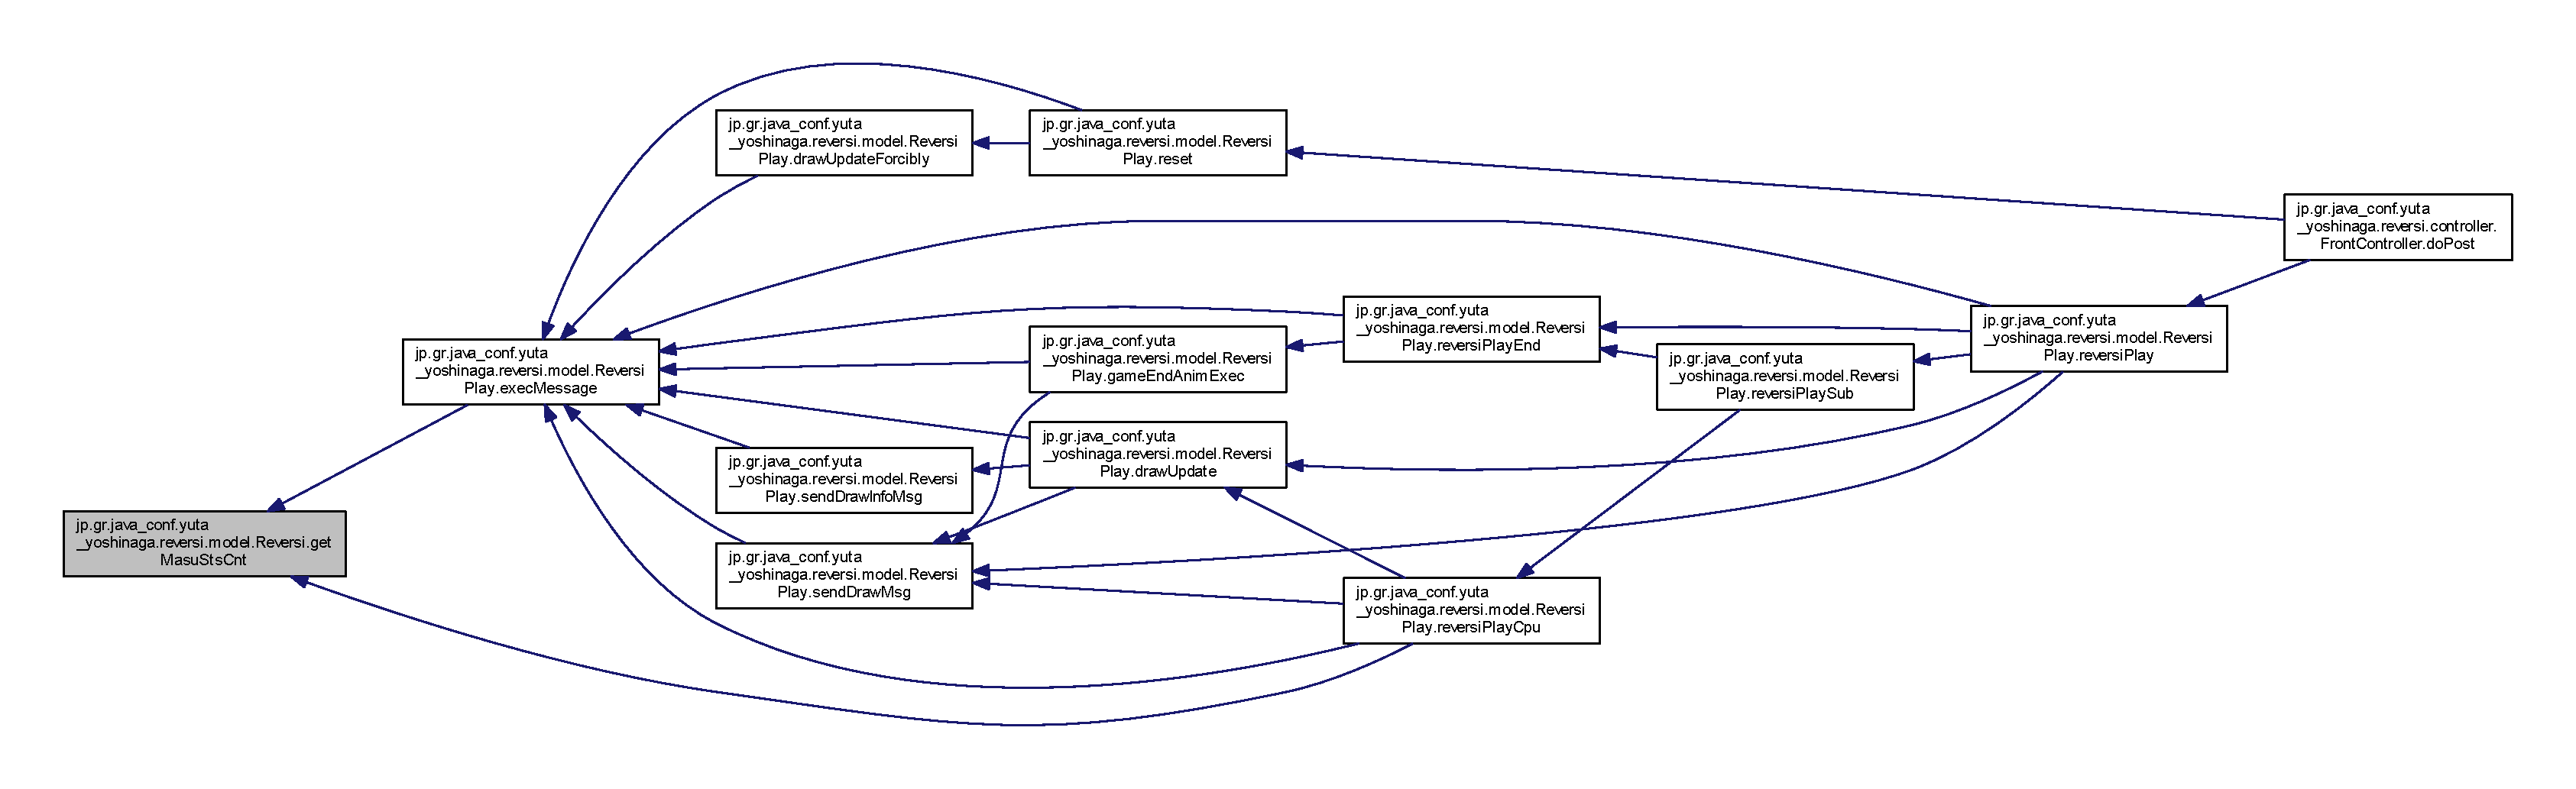
\includegraphics[width=350pt]{classjp_1_1gr_1_1java__conf_1_1yuta__yoshinaga_1_1reversi_1_1model_1_1_reversi_a1a528710342faba65975f4768d24b129_icgraph}
\end{center}
\end{figure}
\mbox{\Hypertarget{classjp_1_1gr_1_1java__conf_1_1yuta__yoshinaga_1_1reversi_1_1model_1_1_reversi_a055f20327e781b1f6807dba0baa1e51b}\label{classjp_1_1gr_1_1java__conf_1_1yuta__yoshinaga_1_1reversi_1_1model_1_1_reversi_a055f20327e781b1f6807dba0baa1e51b}} 
\index{jp\+::gr\+::java\+\_\+conf\+::yuta\+\_\+yoshinaga\+::reversi\+::model\+::\+Reversi@{jp\+::gr\+::java\+\_\+conf\+::yuta\+\_\+yoshinaga\+::reversi\+::model\+::\+Reversi}!get\+Masu\+Sts\+Ena@{get\+Masu\+Sts\+Ena}}
\index{get\+Masu\+Sts\+Ena@{get\+Masu\+Sts\+Ena}!jp\+::gr\+::java\+\_\+conf\+::yuta\+\_\+yoshinaga\+::reversi\+::model\+::\+Reversi@{jp\+::gr\+::java\+\_\+conf\+::yuta\+\_\+yoshinaga\+::reversi\+::model\+::\+Reversi}}
\subsubsection{\texorpdfstring{get\+Masu\+Sts\+Ena()}{getMasuStsEna()}}
{\footnotesize\ttfamily public int jp.\+gr.\+java\+\_\+conf.\+yuta\+\_\+yoshinaga.\+reversi.\+model.\+Reversi.\+get\+Masu\+Sts\+Ena (\begin{DoxyParamCaption}\item[{int}]{color,  }\item[{int}]{y,  }\item[{int}]{x }\end{DoxyParamCaption})}



指定座標に指定色を置けるかチェック 


\begin{DoxyParams}[1]{Parameters}
\mbox{\tt in}  & {\em int} & color コマ色 \\
\hline
\mbox{\tt in}  & {\em int} & y マスの\+Y座標 \\
\hline
\mbox{\tt in}  & {\em int} & x マスの\+X座標 \\
\hline
\end{DoxyParams}
\begin{DoxyReturn}{Returns}
1 \+: 成功 それ以外 \+: 失敗 
\end{DoxyReturn}
\begin{DoxyAuthor}{Author}
Yuta Yoshinaga 
\end{DoxyAuthor}
\begin{DoxyDate}{Date}
2018.\+04.\+01 
\end{DoxyDate}


Definition at line 1401 of file Reversi.\+java.



Referenced by jp.\+gr.\+java\+\_\+conf.\+yuta\+\_\+yoshinaga.\+reversi.\+model.\+Reversi.\+Analysis\+Reversi\+Black(), jp.\+gr.\+java\+\_\+conf.\+yuta\+\_\+yoshinaga.\+reversi.\+model.\+Reversi.\+Analysis\+Reversi\+White(), jp.\+gr.\+java\+\_\+conf.\+yuta\+\_\+yoshinaga.\+reversi.\+model.\+Reversi\+Play.\+exec\+Message(), jp.\+gr.\+java\+\_\+conf.\+yuta\+\_\+yoshinaga.\+reversi.\+model.\+Reversi.\+get\+Color\+Ena(), jp.\+gr.\+java\+\_\+conf.\+yuta\+\_\+yoshinaga.\+reversi.\+model.\+Reversi\+Play.\+reversi\+Play\+Cpu(), and jp.\+gr.\+java\+\_\+conf.\+yuta\+\_\+yoshinaga.\+reversi.\+model.\+Reversi.\+set\+Masu\+Sts().

Here is the call graph for this function\+:
\nopagebreak
\begin{figure}[H]
\begin{center}
\leavevmode
\includegraphics[width=350pt]{classjp_1_1gr_1_1java__conf_1_1yuta__yoshinaga_1_1reversi_1_1model_1_1_reversi_a055f20327e781b1f6807dba0baa1e51b_cgraph}
\end{center}
\end{figure}
Here is the caller graph for this function\+:
\nopagebreak
\begin{figure}[H]
\begin{center}
\leavevmode
\includegraphics[width=350pt]{classjp_1_1gr_1_1java__conf_1_1yuta__yoshinaga_1_1reversi_1_1model_1_1_reversi_a055f20327e781b1f6807dba0baa1e51b_icgraph}
\end{center}
\end{figure}
\mbox{\Hypertarget{classjp_1_1gr_1_1java__conf_1_1yuta__yoshinaga_1_1reversi_1_1model_1_1_reversi_a051aca9eb7ac3ce375a6c017fd0eb400}\label{classjp_1_1gr_1_1java__conf_1_1yuta__yoshinaga_1_1reversi_1_1model_1_1_reversi_a051aca9eb7ac3ce375a6c017fd0eb400}} 
\index{jp\+::gr\+::java\+\_\+conf\+::yuta\+\_\+yoshinaga\+::reversi\+::model\+::\+Reversi@{jp\+::gr\+::java\+\_\+conf\+::yuta\+\_\+yoshinaga\+::reversi\+::model\+::\+Reversi}!get\+Masu\+Sts\+Old@{get\+Masu\+Sts\+Old}}
\index{get\+Masu\+Sts\+Old@{get\+Masu\+Sts\+Old}!jp\+::gr\+::java\+\_\+conf\+::yuta\+\_\+yoshinaga\+::reversi\+::model\+::\+Reversi@{jp\+::gr\+::java\+\_\+conf\+::yuta\+\_\+yoshinaga\+::reversi\+::model\+::\+Reversi}}
\subsubsection{\texorpdfstring{get\+Masu\+Sts\+Old()}{getMasuStsOld()}}
{\footnotesize\ttfamily int jp.\+gr.\+java\+\_\+conf.\+yuta\+\_\+yoshinaga.\+reversi.\+model.\+Reversi.\+get\+Masu\+Sts\+Old (\begin{DoxyParamCaption}\item[{int}]{y,  }\item[{int}]{x }\end{DoxyParamCaption})}



以前のマスステータスを取得 


\begin{DoxyParams}[1]{Parameters}
\mbox{\tt in}  & {\em int} & y 取得するマスの\+Y座標 \\
\hline
\mbox{\tt in}  & {\em int} & x 取得するマスの\+X座標 \\
\hline
\end{DoxyParams}
\begin{DoxyReturn}{Returns}
-\/1 \+: 失敗 それ以外 \+: マスステータス 
\end{DoxyReturn}
\begin{DoxyAuthor}{Author}
Yuta Yoshinaga 
\end{DoxyAuthor}
\begin{DoxyDate}{Date}
2017.\+10.\+20 
\end{DoxyDate}


Definition at line 1383 of file Reversi.\+java.



Referenced by jp.\+gr.\+java\+\_\+conf.\+yuta\+\_\+yoshinaga.\+reversi.\+model.\+Reversi\+Play.\+draw\+Update().

Here is the call graph for this function\+:
\nopagebreak
\begin{figure}[H]
\begin{center}
\leavevmode
\includegraphics[width=350pt]{classjp_1_1gr_1_1java__conf_1_1yuta__yoshinaga_1_1reversi_1_1model_1_1_reversi_a051aca9eb7ac3ce375a6c017fd0eb400_cgraph}
\end{center}
\end{figure}
Here is the caller graph for this function\+:
\nopagebreak
\begin{figure}[H]
\begin{center}
\leavevmode
\includegraphics[width=350pt]{classjp_1_1gr_1_1java__conf_1_1yuta__yoshinaga_1_1reversi_1_1model_1_1_reversi_a051aca9eb7ac3ce375a6c017fd0eb400_icgraph}
\end{center}
\end{figure}
\mbox{\Hypertarget{classjp_1_1gr_1_1java__conf_1_1yuta__yoshinaga_1_1reversi_1_1model_1_1_reversi_a9eca6c8f158433303079e333a29ee564}\label{classjp_1_1gr_1_1java__conf_1_1yuta__yoshinaga_1_1reversi_1_1model_1_1_reversi_a9eca6c8f158433303079e333a29ee564}} 
\index{jp\+::gr\+::java\+\_\+conf\+::yuta\+\_\+yoshinaga\+::reversi\+::model\+::\+Reversi@{jp\+::gr\+::java\+\_\+conf\+::yuta\+\_\+yoshinaga\+::reversi\+::model\+::\+Reversi}!getm\+Masu\+Bet\+CntB@{getm\+Masu\+Bet\+CntB}}
\index{getm\+Masu\+Bet\+CntB@{getm\+Masu\+Bet\+CntB}!jp\+::gr\+::java\+\_\+conf\+::yuta\+\_\+yoshinaga\+::reversi\+::model\+::\+Reversi@{jp\+::gr\+::java\+\_\+conf\+::yuta\+\_\+yoshinaga\+::reversi\+::model\+::\+Reversi}}
\subsubsection{\texorpdfstring{getm\+Masu\+Bet\+Cnt\+B()}{getmMasuBetCntB()}}
{\footnotesize\ttfamily int jp.\+gr.\+java\+\_\+conf.\+yuta\+\_\+yoshinaga.\+reversi.\+model.\+Reversi.\+getm\+Masu\+Bet\+CntB (\begin{DoxyParamCaption}{ }\end{DoxyParamCaption})}



ゲッター 

\begin{DoxyReturn}{Returns}
int m\+Masu\+Bet\+CntB 
\end{DoxyReturn}
\begin{DoxyAuthor}{Author}
Yuta Yoshinaga 
\end{DoxyAuthor}
\begin{DoxyDate}{Date}
2018.\+04.\+01 
\end{DoxyDate}


Definition at line 258 of file Reversi.\+java.

\mbox{\Hypertarget{classjp_1_1gr_1_1java__conf_1_1yuta__yoshinaga_1_1reversi_1_1model_1_1_reversi_a0c8bd1c479d27a1531b99baa9af52fb6}\label{classjp_1_1gr_1_1java__conf_1_1yuta__yoshinaga_1_1reversi_1_1model_1_1_reversi_a0c8bd1c479d27a1531b99baa9af52fb6}} 
\index{jp\+::gr\+::java\+\_\+conf\+::yuta\+\_\+yoshinaga\+::reversi\+::model\+::\+Reversi@{jp\+::gr\+::java\+\_\+conf\+::yuta\+\_\+yoshinaga\+::reversi\+::model\+::\+Reversi}!getm\+Masu\+Bet\+CntW@{getm\+Masu\+Bet\+CntW}}
\index{getm\+Masu\+Bet\+CntW@{getm\+Masu\+Bet\+CntW}!jp\+::gr\+::java\+\_\+conf\+::yuta\+\_\+yoshinaga\+::reversi\+::model\+::\+Reversi@{jp\+::gr\+::java\+\_\+conf\+::yuta\+\_\+yoshinaga\+::reversi\+::model\+::\+Reversi}}
\subsubsection{\texorpdfstring{getm\+Masu\+Bet\+Cnt\+W()}{getmMasuBetCntW()}}
{\footnotesize\ttfamily int jp.\+gr.\+java\+\_\+conf.\+yuta\+\_\+yoshinaga.\+reversi.\+model.\+Reversi.\+getm\+Masu\+Bet\+CntW (\begin{DoxyParamCaption}{ }\end{DoxyParamCaption})}



ゲッター 

\begin{DoxyReturn}{Returns}
int m\+Masu\+Bet\+CntW 
\end{DoxyReturn}
\begin{DoxyAuthor}{Author}
Yuta Yoshinaga 
\end{DoxyAuthor}
\begin{DoxyDate}{Date}
2018.\+04.\+01 
\end{DoxyDate}


Definition at line 433 of file Reversi.\+java.

\mbox{\Hypertarget{classjp_1_1gr_1_1java__conf_1_1yuta__yoshinaga_1_1reversi_1_1model_1_1_reversi_a9ee4f16f9fedcea48c44f81e8ad73f81}\label{classjp_1_1gr_1_1java__conf_1_1yuta__yoshinaga_1_1reversi_1_1model_1_1_reversi_a9ee4f16f9fedcea48c44f81e8ad73f81}} 
\index{jp\+::gr\+::java\+\_\+conf\+::yuta\+\_\+yoshinaga\+::reversi\+::model\+::\+Reversi@{jp\+::gr\+::java\+\_\+conf\+::yuta\+\_\+yoshinaga\+::reversi\+::model\+::\+Reversi}!getm\+Masu\+Cnt@{getm\+Masu\+Cnt}}
\index{getm\+Masu\+Cnt@{getm\+Masu\+Cnt}!jp\+::gr\+::java\+\_\+conf\+::yuta\+\_\+yoshinaga\+::reversi\+::model\+::\+Reversi@{jp\+::gr\+::java\+\_\+conf\+::yuta\+\_\+yoshinaga\+::reversi\+::model\+::\+Reversi}}
\subsubsection{\texorpdfstring{getm\+Masu\+Cnt()}{getmMasuCnt()}}
{\footnotesize\ttfamily int jp.\+gr.\+java\+\_\+conf.\+yuta\+\_\+yoshinaga.\+reversi.\+model.\+Reversi.\+getm\+Masu\+Cnt (\begin{DoxyParamCaption}{ }\end{DoxyParamCaption})}



ゲッター 

\begin{DoxyReturn}{Returns}
int m\+Masu\+Cnt 
\end{DoxyReturn}
\begin{DoxyAuthor}{Author}
Yuta Yoshinaga 
\end{DoxyAuthor}
\begin{DoxyDate}{Date}
2018.\+04.\+01 
\end{DoxyDate}


Definition at line 458 of file Reversi.\+java.

\mbox{\Hypertarget{classjp_1_1gr_1_1java__conf_1_1yuta__yoshinaga_1_1reversi_1_1model_1_1_reversi_a1991b683bec4721f4228a262423790a9}\label{classjp_1_1gr_1_1java__conf_1_1yuta__yoshinaga_1_1reversi_1_1model_1_1_reversi_a1991b683bec4721f4228a262423790a9}} 
\index{jp\+::gr\+::java\+\_\+conf\+::yuta\+\_\+yoshinaga\+::reversi\+::model\+::\+Reversi@{jp\+::gr\+::java\+\_\+conf\+::yuta\+\_\+yoshinaga\+::reversi\+::model\+::\+Reversi}!getm\+Masu\+Cnt\+Max@{getm\+Masu\+Cnt\+Max}}
\index{getm\+Masu\+Cnt\+Max@{getm\+Masu\+Cnt\+Max}!jp\+::gr\+::java\+\_\+conf\+::yuta\+\_\+yoshinaga\+::reversi\+::model\+::\+Reversi@{jp\+::gr\+::java\+\_\+conf\+::yuta\+\_\+yoshinaga\+::reversi\+::model\+::\+Reversi}}
\subsubsection{\texorpdfstring{getm\+Masu\+Cnt\+Max()}{getmMasuCntMax()}}
{\footnotesize\ttfamily int jp.\+gr.\+java\+\_\+conf.\+yuta\+\_\+yoshinaga.\+reversi.\+model.\+Reversi.\+getm\+Masu\+Cnt\+Max (\begin{DoxyParamCaption}{ }\end{DoxyParamCaption})}



ゲッター 

\begin{DoxyReturn}{Returns}
int m\+Masu\+Cnt\+Max 
\end{DoxyReturn}
\begin{DoxyAuthor}{Author}
Yuta Yoshinaga 
\end{DoxyAuthor}
\begin{DoxyDate}{Date}
2018.\+04.\+01 
\end{DoxyDate}


Definition at line 483 of file Reversi.\+java.

\mbox{\Hypertarget{classjp_1_1gr_1_1java__conf_1_1yuta__yoshinaga_1_1reversi_1_1model_1_1_reversi_a0bc45b287c439f0fcce73779a91be405}\label{classjp_1_1gr_1_1java__conf_1_1yuta__yoshinaga_1_1reversi_1_1model_1_1_reversi_a0bc45b287c439f0fcce73779a91be405}} 
\index{jp\+::gr\+::java\+\_\+conf\+::yuta\+\_\+yoshinaga\+::reversi\+::model\+::\+Reversi@{jp\+::gr\+::java\+\_\+conf\+::yuta\+\_\+yoshinaga\+::reversi\+::model\+::\+Reversi}!getm\+Masu\+Hist\+Cur@{getm\+Masu\+Hist\+Cur}}
\index{getm\+Masu\+Hist\+Cur@{getm\+Masu\+Hist\+Cur}!jp\+::gr\+::java\+\_\+conf\+::yuta\+\_\+yoshinaga\+::reversi\+::model\+::\+Reversi@{jp\+::gr\+::java\+\_\+conf\+::yuta\+\_\+yoshinaga\+::reversi\+::model\+::\+Reversi}}
\subsubsection{\texorpdfstring{getm\+Masu\+Hist\+Cur()}{getmMasuHistCur()}}
{\footnotesize\ttfamily int jp.\+gr.\+java\+\_\+conf.\+yuta\+\_\+yoshinaga.\+reversi.\+model.\+Reversi.\+getm\+Masu\+Hist\+Cur (\begin{DoxyParamCaption}{ }\end{DoxyParamCaption})}



ゲッター 

\begin{DoxyReturn}{Returns}
int m\+Masu\+Hist\+Cur 
\end{DoxyReturn}
\begin{DoxyAuthor}{Author}
Yuta Yoshinaga 
\end{DoxyAuthor}
\begin{DoxyDate}{Date}
2018.\+04.\+01 
\end{DoxyDate}


Definition at line 533 of file Reversi.\+java.

\mbox{\Hypertarget{classjp_1_1gr_1_1java__conf_1_1yuta__yoshinaga_1_1reversi_1_1model_1_1_reversi_ad2c4e4e56738790789c00c7ce53d1f24}\label{classjp_1_1gr_1_1java__conf_1_1yuta__yoshinaga_1_1reversi_1_1model_1_1_reversi_ad2c4e4e56738790789c00c7ce53d1f24}} 
\index{jp\+::gr\+::java\+\_\+conf\+::yuta\+\_\+yoshinaga\+::reversi\+::model\+::\+Reversi@{jp\+::gr\+::java\+\_\+conf\+::yuta\+\_\+yoshinaga\+::reversi\+::model\+::\+Reversi}!getm\+Masu\+Point\+CntB@{getm\+Masu\+Point\+CntB}}
\index{getm\+Masu\+Point\+CntB@{getm\+Masu\+Point\+CntB}!jp\+::gr\+::java\+\_\+conf\+::yuta\+\_\+yoshinaga\+::reversi\+::model\+::\+Reversi@{jp\+::gr\+::java\+\_\+conf\+::yuta\+\_\+yoshinaga\+::reversi\+::model\+::\+Reversi}}
\subsubsection{\texorpdfstring{getm\+Masu\+Point\+Cnt\+B()}{getmMasuPointCntB()}}
{\footnotesize\ttfamily int jp.\+gr.\+java\+\_\+conf.\+yuta\+\_\+yoshinaga.\+reversi.\+model.\+Reversi.\+getm\+Masu\+Point\+CntB (\begin{DoxyParamCaption}{ }\end{DoxyParamCaption})}



ゲッター 

\begin{DoxyReturn}{Returns}
int m\+Masu\+Point\+CntB 
\end{DoxyReturn}
\begin{DoxyAuthor}{Author}
Yuta Yoshinaga 
\end{DoxyAuthor}
\begin{DoxyDate}{Date}
2018.\+04.\+01 
\end{DoxyDate}


Definition at line 233 of file Reversi.\+java.

\mbox{\Hypertarget{classjp_1_1gr_1_1java__conf_1_1yuta__yoshinaga_1_1reversi_1_1model_1_1_reversi_a4a8980c09fba0b53d19efd195f66338e}\label{classjp_1_1gr_1_1java__conf_1_1yuta__yoshinaga_1_1reversi_1_1model_1_1_reversi_a4a8980c09fba0b53d19efd195f66338e}} 
\index{jp\+::gr\+::java\+\_\+conf\+::yuta\+\_\+yoshinaga\+::reversi\+::model\+::\+Reversi@{jp\+::gr\+::java\+\_\+conf\+::yuta\+\_\+yoshinaga\+::reversi\+::model\+::\+Reversi}!getm\+Masu\+Point\+CntW@{getm\+Masu\+Point\+CntW}}
\index{getm\+Masu\+Point\+CntW@{getm\+Masu\+Point\+CntW}!jp\+::gr\+::java\+\_\+conf\+::yuta\+\_\+yoshinaga\+::reversi\+::model\+::\+Reversi@{jp\+::gr\+::java\+\_\+conf\+::yuta\+\_\+yoshinaga\+::reversi\+::model\+::\+Reversi}}
\subsubsection{\texorpdfstring{getm\+Masu\+Point\+Cnt\+W()}{getmMasuPointCntW()}}
{\footnotesize\ttfamily int jp.\+gr.\+java\+\_\+conf.\+yuta\+\_\+yoshinaga.\+reversi.\+model.\+Reversi.\+getm\+Masu\+Point\+CntW (\begin{DoxyParamCaption}{ }\end{DoxyParamCaption})}



ゲッター 

\begin{DoxyReturn}{Returns}
int m\+Masu\+Point\+CntW 
\end{DoxyReturn}
\begin{DoxyAuthor}{Author}
Yuta Yoshinaga 
\end{DoxyAuthor}
\begin{DoxyDate}{Date}
2018.\+04.\+01 
\end{DoxyDate}


Definition at line 408 of file Reversi.\+java.

\mbox{\Hypertarget{classjp_1_1gr_1_1java__conf_1_1yuta__yoshinaga_1_1reversi_1_1model_1_1_reversi_ab180757b310c3a72cf159043ba0dc09e}\label{classjp_1_1gr_1_1java__conf_1_1yuta__yoshinaga_1_1reversi_1_1model_1_1_reversi_ab180757b310c3a72cf159043ba0dc09e}} 
\index{jp\+::gr\+::java\+\_\+conf\+::yuta\+\_\+yoshinaga\+::reversi\+::model\+::\+Reversi@{jp\+::gr\+::java\+\_\+conf\+::yuta\+\_\+yoshinaga\+::reversi\+::model\+::\+Reversi}!get\+Point@{get\+Point}}
\index{get\+Point@{get\+Point}!jp\+::gr\+::java\+\_\+conf\+::yuta\+\_\+yoshinaga\+::reversi\+::model\+::\+Reversi@{jp\+::gr\+::java\+\_\+conf\+::yuta\+\_\+yoshinaga\+::reversi\+::model\+::\+Reversi}}
\subsubsection{\texorpdfstring{get\+Point()}{getPoint()}}
{\footnotesize\ttfamily public \hyperlink{classjp_1_1gr_1_1java__conf_1_1yuta__yoshinaga_1_1reversi_1_1model_1_1_reversi_point}{Reversi\+Point} jp.\+gr.\+java\+\_\+conf.\+yuta\+\_\+yoshinaga.\+reversi.\+model.\+Reversi.\+get\+Point (\begin{DoxyParamCaption}\item[{int}]{color,  }\item[{int}]{num }\end{DoxyParamCaption})}



ポイント座標取得 


\begin{DoxyParams}[1]{Parameters}
\mbox{\tt in}  & {\em int} & color コマ色 \\
\hline
\mbox{\tt in}  & {\em int} & num ポイント \\
\hline
\end{DoxyParams}
\begin{DoxyReturn}{Returns}
ポイント座標 null \+: 失敗 
\end{DoxyReturn}
\begin{DoxyAuthor}{Author}
Yuta Yoshinaga 
\end{DoxyAuthor}
\begin{DoxyDate}{Date}
2018.\+04.\+01 
\end{DoxyDate}


Definition at line 1560 of file Reversi.\+java.



Referenced by jp.\+gr.\+java\+\_\+conf.\+yuta\+\_\+yoshinaga.\+reversi.\+model.\+Reversi\+Play.\+reset(), and jp.\+gr.\+java\+\_\+conf.\+yuta\+\_\+yoshinaga.\+reversi.\+model.\+Reversi\+Play.\+reversi\+Play\+Cpu().

Here is the call graph for this function\+:
\nopagebreak
\begin{figure}[H]
\begin{center}
\leavevmode
\includegraphics[width=350pt]{classjp_1_1gr_1_1java__conf_1_1yuta__yoshinaga_1_1reversi_1_1model_1_1_reversi_ab180757b310c3a72cf159043ba0dc09e_cgraph}
\end{center}
\end{figure}
Here is the caller graph for this function\+:
\nopagebreak
\begin{figure}[H]
\begin{center}
\leavevmode
\includegraphics[width=350pt]{classjp_1_1gr_1_1java__conf_1_1yuta__yoshinaga_1_1reversi_1_1model_1_1_reversi_ab180757b310c3a72cf159043ba0dc09e_icgraph}
\end{center}
\end{figure}
\mbox{\Hypertarget{classjp_1_1gr_1_1java__conf_1_1yuta__yoshinaga_1_1reversi_1_1model_1_1_reversi_a6da3f67c0468cf59ba6ceb796133c921}\label{classjp_1_1gr_1_1java__conf_1_1yuta__yoshinaga_1_1reversi_1_1model_1_1_reversi_a6da3f67c0468cf59ba6ceb796133c921}} 
\index{jp\+::gr\+::java\+\_\+conf\+::yuta\+\_\+yoshinaga\+::reversi\+::model\+::\+Reversi@{jp\+::gr\+::java\+\_\+conf\+::yuta\+\_\+yoshinaga\+::reversi\+::model\+::\+Reversi}!get\+Point\+Anz@{get\+Point\+Anz}}
\index{get\+Point\+Anz@{get\+Point\+Anz}!jp\+::gr\+::java\+\_\+conf\+::yuta\+\_\+yoshinaga\+::reversi\+::model\+::\+Reversi@{jp\+::gr\+::java\+\_\+conf\+::yuta\+\_\+yoshinaga\+::reversi\+::model\+::\+Reversi}}
\subsubsection{\texorpdfstring{get\+Point\+Anz()}{getPointAnz()}}
{\footnotesize\ttfamily public \hyperlink{classjp_1_1gr_1_1java__conf_1_1yuta__yoshinaga_1_1reversi_1_1model_1_1_reversi_anz}{Reversi\+Anz} jp.\+gr.\+java\+\_\+conf.\+yuta\+\_\+yoshinaga.\+reversi.\+model.\+Reversi.\+get\+Point\+Anz (\begin{DoxyParamCaption}\item[{int}]{color,  }\item[{int}]{y,  }\item[{int}]{x }\end{DoxyParamCaption})}



ポイント座標解析取得 


\begin{DoxyParams}[1]{Parameters}
\mbox{\tt in}  & {\em int} & color コマ色 \\
\hline
\mbox{\tt in}  & {\em int} & y マスの\+Y座標 \\
\hline
\mbox{\tt in}  & {\em int} & x マスの\+X座標 \\
\hline
\end{DoxyParams}
\begin{DoxyReturn}{Returns}
ポイント座標解析 null \+: 失敗 
\end{DoxyReturn}
\begin{DoxyAuthor}{Author}
Yuta Yoshinaga 
\end{DoxyAuthor}
\begin{DoxyDate}{Date}
2018.\+04.\+01 
\end{DoxyDate}


Definition at line 1672 of file Reversi.\+java.



Referenced by jp.\+gr.\+java\+\_\+conf.\+yuta\+\_\+yoshinaga.\+reversi.\+model.\+Reversi\+Play.\+reversi\+Play\+Cpu().

Here is the call graph for this function\+:
\nopagebreak
\begin{figure}[H]
\begin{center}
\leavevmode
\includegraphics[width=350pt]{classjp_1_1gr_1_1java__conf_1_1yuta__yoshinaga_1_1reversi_1_1model_1_1_reversi_a6da3f67c0468cf59ba6ceb796133c921_cgraph}
\end{center}
\end{figure}
Here is the caller graph for this function\+:
\nopagebreak
\begin{figure}[H]
\begin{center}
\leavevmode
\includegraphics[width=350pt]{classjp_1_1gr_1_1java__conf_1_1yuta__yoshinaga_1_1reversi_1_1model_1_1_reversi_a6da3f67c0468cf59ba6ceb796133c921_icgraph}
\end{center}
\end{figure}
\mbox{\Hypertarget{classjp_1_1gr_1_1java__conf_1_1yuta__yoshinaga_1_1reversi_1_1model_1_1_reversi_a8ab289d67a725a30e92411c90b755bd8}\label{classjp_1_1gr_1_1java__conf_1_1yuta__yoshinaga_1_1reversi_1_1model_1_1_reversi_a8ab289d67a725a30e92411c90b755bd8}} 
\index{jp\+::gr\+::java\+\_\+conf\+::yuta\+\_\+yoshinaga\+::reversi\+::model\+::\+Reversi@{jp\+::gr\+::java\+\_\+conf\+::yuta\+\_\+yoshinaga\+::reversi\+::model\+::\+Reversi}!get\+Point\+Cnt@{get\+Point\+Cnt}}
\index{get\+Point\+Cnt@{get\+Point\+Cnt}!jp\+::gr\+::java\+\_\+conf\+::yuta\+\_\+yoshinaga\+::reversi\+::model\+::\+Reversi@{jp\+::gr\+::java\+\_\+conf\+::yuta\+\_\+yoshinaga\+::reversi\+::model\+::\+Reversi}}
\subsubsection{\texorpdfstring{get\+Point\+Cnt()}{getPointCnt()}}
{\footnotesize\ttfamily public int jp.\+gr.\+java\+\_\+conf.\+yuta\+\_\+yoshinaga.\+reversi.\+model.\+Reversi.\+get\+Point\+Cnt (\begin{DoxyParamCaption}\item[{int}]{color }\end{DoxyParamCaption})}



ポイント座標数取得 


\begin{DoxyParams}[1]{Parameters}
\mbox{\tt in}  & {\em int} & color コマ色 \\
\hline
\end{DoxyParams}
\begin{DoxyReturn}{Returns}
ポイント座標数取得 
\end{DoxyReturn}
\begin{DoxyAuthor}{Author}
Yuta Yoshinaga 
\end{DoxyAuthor}
\begin{DoxyDate}{Date}
2018.\+04.\+01 
\end{DoxyDate}


Definition at line 1579 of file Reversi.\+java.



Referenced by jp.\+gr.\+java\+\_\+conf.\+yuta\+\_\+yoshinaga.\+reversi.\+model.\+Reversi.\+Analysis\+Reversi\+Black(), jp.\+gr.\+java\+\_\+conf.\+yuta\+\_\+yoshinaga.\+reversi.\+model.\+Reversi.\+Analysis\+Reversi\+White(), jp.\+gr.\+java\+\_\+conf.\+yuta\+\_\+yoshinaga.\+reversi.\+model.\+Reversi\+Play.\+reset(), and jp.\+gr.\+java\+\_\+conf.\+yuta\+\_\+yoshinaga.\+reversi.\+model.\+Reversi\+Play.\+reversi\+Play\+Cpu().

Here is the caller graph for this function\+:
\nopagebreak
\begin{figure}[H]
\begin{center}
\leavevmode
\includegraphics[width=350pt]{classjp_1_1gr_1_1java__conf_1_1yuta__yoshinaga_1_1reversi_1_1model_1_1_reversi_a8ab289d67a725a30e92411c90b755bd8_icgraph}
\end{center}
\end{figure}
\mbox{\Hypertarget{classjp_1_1gr_1_1java__conf_1_1yuta__yoshinaga_1_1reversi_1_1model_1_1_reversi_a9929ed36140ddc25923ede99f86564c3}\label{classjp_1_1gr_1_1java__conf_1_1yuta__yoshinaga_1_1reversi_1_1model_1_1_reversi_a9929ed36140ddc25923ede99f86564c3}} 
\index{jp\+::gr\+::java\+\_\+conf\+::yuta\+\_\+yoshinaga\+::reversi\+::model\+::\+Reversi@{jp\+::gr\+::java\+\_\+conf\+::yuta\+\_\+yoshinaga\+::reversi\+::model\+::\+Reversi}!make\+Masu\+Sts@{make\+Masu\+Sts}}
\index{make\+Masu\+Sts@{make\+Masu\+Sts}!jp\+::gr\+::java\+\_\+conf\+::yuta\+\_\+yoshinaga\+::reversi\+::model\+::\+Reversi@{jp\+::gr\+::java\+\_\+conf\+::yuta\+\_\+yoshinaga\+::reversi\+::model\+::\+Reversi}}
\subsubsection{\texorpdfstring{make\+Masu\+Sts()}{makeMasuSts()}}
{\footnotesize\ttfamily private int jp.\+gr.\+java\+\_\+conf.\+yuta\+\_\+yoshinaga.\+reversi.\+model.\+Reversi.\+make\+Masu\+Sts (\begin{DoxyParamCaption}\item[{int}]{color }\end{DoxyParamCaption})\hspace{0.3cm}{\ttfamily [private]}}



各コマの置ける場所等のステータス作成 


\begin{DoxyParams}[1]{Parameters}
\mbox{\tt in}  & {\em int} & color ステータスを作成するコマ \\
\hline
\end{DoxyParams}
\begin{DoxyReturn}{Returns}
ありません 
\end{DoxyReturn}
\begin{DoxyAuthor}{Author}
Yuta Yoshinaga 
\end{DoxyAuthor}
\begin{DoxyDate}{Date}
2018.\+04.\+01 
\end{DoxyDate}


Definition at line 660 of file Reversi.\+java.



Referenced by jp.\+gr.\+java\+\_\+conf.\+yuta\+\_\+yoshinaga.\+reversi.\+model.\+Reversi.\+Analysis\+Reversi(), jp.\+gr.\+java\+\_\+conf.\+yuta\+\_\+yoshinaga.\+reversi.\+model.\+Reversi.\+Analysis\+Reversi\+Black(), jp.\+gr.\+java\+\_\+conf.\+yuta\+\_\+yoshinaga.\+reversi.\+model.\+Reversi.\+Analysis\+Reversi\+White(), jp.\+gr.\+java\+\_\+conf.\+yuta\+\_\+yoshinaga.\+reversi.\+model.\+Reversi.\+reset(), and jp.\+gr.\+java\+\_\+conf.\+yuta\+\_\+yoshinaga.\+reversi.\+model.\+Reversi.\+set\+Masu\+Sts().

Here is the call graph for this function\+:
\nopagebreak
\begin{figure}[H]
\begin{center}
\leavevmode
\includegraphics[width=350pt]{classjp_1_1gr_1_1java__conf_1_1yuta__yoshinaga_1_1reversi_1_1model_1_1_reversi_a9929ed36140ddc25923ede99f86564c3_cgraph}
\end{center}
\end{figure}
Here is the caller graph for this function\+:
\nopagebreak
\begin{figure}[H]
\begin{center}
\leavevmode
\includegraphics[width=350pt]{classjp_1_1gr_1_1java__conf_1_1yuta__yoshinaga_1_1reversi_1_1model_1_1_reversi_a9929ed36140ddc25923ede99f86564c3_icgraph}
\end{center}
\end{figure}
\mbox{\Hypertarget{classjp_1_1gr_1_1java__conf_1_1yuta__yoshinaga_1_1reversi_1_1model_1_1_reversi_a497552844cbae36207f2d8c836a26b8e}\label{classjp_1_1gr_1_1java__conf_1_1yuta__yoshinaga_1_1reversi_1_1model_1_1_reversi_a497552844cbae36207f2d8c836a26b8e}} 
\index{jp\+::gr\+::java\+\_\+conf\+::yuta\+\_\+yoshinaga\+::reversi\+::model\+::\+Reversi@{jp\+::gr\+::java\+\_\+conf\+::yuta\+\_\+yoshinaga\+::reversi\+::model\+::\+Reversi}!reset@{reset}}
\index{reset@{reset}!jp\+::gr\+::java\+\_\+conf\+::yuta\+\_\+yoshinaga\+::reversi\+::model\+::\+Reversi@{jp\+::gr\+::java\+\_\+conf\+::yuta\+\_\+yoshinaga\+::reversi\+::model\+::\+Reversi}}
\subsubsection{\texorpdfstring{reset()}{reset()}}
{\footnotesize\ttfamily public void jp.\+gr.\+java\+\_\+conf.\+yuta\+\_\+yoshinaga.\+reversi.\+model.\+Reversi.\+reset (\begin{DoxyParamCaption}{ }\end{DoxyParamCaption})}



リセット 

\begin{DoxyReturn}{Returns}
ありません 
\end{DoxyReturn}
\begin{DoxyAuthor}{Author}
Yuta Yoshinaga 
\end{DoxyAuthor}
\begin{DoxyDate}{Date}
2018.\+04.\+01 
\end{DoxyDate}


Definition at line 628 of file Reversi.\+java.



Referenced by jp.\+gr.\+java\+\_\+conf.\+yuta\+\_\+yoshinaga.\+reversi.\+model.\+Reversi\+Play.\+reset(), jp.\+gr.\+java\+\_\+conf.\+yuta\+\_\+yoshinaga.\+reversi.\+model.\+Reversi.\+Reversi(), and jp.\+gr.\+java\+\_\+conf.\+yuta\+\_\+yoshinaga.\+reversi.\+model.\+Reversi.\+set\+Masu\+Cnt().

Here is the call graph for this function\+:
\nopagebreak
\begin{figure}[H]
\begin{center}
\leavevmode
\includegraphics[width=350pt]{classjp_1_1gr_1_1java__conf_1_1yuta__yoshinaga_1_1reversi_1_1model_1_1_reversi_a497552844cbae36207f2d8c836a26b8e_cgraph}
\end{center}
\end{figure}
Here is the caller graph for this function\+:
\nopagebreak
\begin{figure}[H]
\begin{center}
\leavevmode
\includegraphics[width=350pt]{classjp_1_1gr_1_1java__conf_1_1yuta__yoshinaga_1_1reversi_1_1model_1_1_reversi_a497552844cbae36207f2d8c836a26b8e_icgraph}
\end{center}
\end{figure}
\mbox{\Hypertarget{classjp_1_1gr_1_1java__conf_1_1yuta__yoshinaga_1_1reversi_1_1model_1_1_reversi_a3c63579c27513dffc555416388f8530a}\label{classjp_1_1gr_1_1java__conf_1_1yuta__yoshinaga_1_1reversi_1_1model_1_1_reversi_a3c63579c27513dffc555416388f8530a}} 
\index{jp\+::gr\+::java\+\_\+conf\+::yuta\+\_\+yoshinaga\+::reversi\+::model\+::\+Reversi@{jp\+::gr\+::java\+\_\+conf\+::yuta\+\_\+yoshinaga\+::reversi\+::model\+::\+Reversi}!rev\+Masu\+Sts@{rev\+Masu\+Sts}}
\index{rev\+Masu\+Sts@{rev\+Masu\+Sts}!jp\+::gr\+::java\+\_\+conf\+::yuta\+\_\+yoshinaga\+::reversi\+::model\+::\+Reversi@{jp\+::gr\+::java\+\_\+conf\+::yuta\+\_\+yoshinaga\+::reversi\+::model\+::\+Reversi}}
\subsubsection{\texorpdfstring{rev\+Masu\+Sts()}{revMasuSts()}}
{\footnotesize\ttfamily private void jp.\+gr.\+java\+\_\+conf.\+yuta\+\_\+yoshinaga.\+reversi.\+model.\+Reversi.\+rev\+Masu\+Sts (\begin{DoxyParamCaption}\item[{int}]{color,  }\item[{int}]{y,  }\item[{int}]{x }\end{DoxyParamCaption})\hspace{0.3cm}{\ttfamily [private]}}



コマをひっくり返す 


\begin{DoxyParams}[1]{Parameters}
\mbox{\tt in}  & {\em int} & color ひっくり返す元コマ \\
\hline
\mbox{\tt in}  & {\em int} & y ひっくり返す元コマの\+Y座標 \\
\hline
\mbox{\tt in}  & {\em int} & x ひっくり返す元コマの\+X座標 \\
\hline
\end{DoxyParams}
\begin{DoxyReturn}{Returns}
ありません 
\end{DoxyReturn}
\begin{DoxyAuthor}{Author}
Yuta Yoshinaga 
\end{DoxyAuthor}
\begin{DoxyDate}{Date}
2018.\+04.\+01 
\end{DoxyDate}


Definition at line 857 of file Reversi.\+java.



Referenced by jp.\+gr.\+java\+\_\+conf.\+yuta\+\_\+yoshinaga.\+reversi.\+model.\+Reversi.\+Analysis\+Reversi\+Black(), jp.\+gr.\+java\+\_\+conf.\+yuta\+\_\+yoshinaga.\+reversi.\+model.\+Reversi.\+Analysis\+Reversi\+White(), and jp.\+gr.\+java\+\_\+conf.\+yuta\+\_\+yoshinaga.\+reversi.\+model.\+Reversi.\+set\+Masu\+Sts().

Here is the caller graph for this function\+:
\nopagebreak
\begin{figure}[H]
\begin{center}
\leavevmode
\includegraphics[width=350pt]{classjp_1_1gr_1_1java__conf_1_1yuta__yoshinaga_1_1reversi_1_1model_1_1_reversi_a3c63579c27513dffc555416388f8530a_icgraph}
\end{center}
\end{figure}
\mbox{\Hypertarget{classjp_1_1gr_1_1java__conf_1_1yuta__yoshinaga_1_1reversi_1_1model_1_1_reversi_a0e9bc15d570635cf024287fbf541b4b9}\label{classjp_1_1gr_1_1java__conf_1_1yuta__yoshinaga_1_1reversi_1_1model_1_1_reversi_a0e9bc15d570635cf024287fbf541b4b9}} 
\index{jp\+::gr\+::java\+\_\+conf\+::yuta\+\_\+yoshinaga\+::reversi\+::model\+::\+Reversi@{jp\+::gr\+::java\+\_\+conf\+::yuta\+\_\+yoshinaga\+::reversi\+::model\+::\+Reversi}!set\+Masu\+Cnt@{set\+Masu\+Cnt}}
\index{set\+Masu\+Cnt@{set\+Masu\+Cnt}!jp\+::gr\+::java\+\_\+conf\+::yuta\+\_\+yoshinaga\+::reversi\+::model\+::\+Reversi@{jp\+::gr\+::java\+\_\+conf\+::yuta\+\_\+yoshinaga\+::reversi\+::model\+::\+Reversi}}
\subsubsection{\texorpdfstring{set\+Masu\+Cnt()}{setMasuCnt()}}
{\footnotesize\ttfamily public int jp.\+gr.\+java\+\_\+conf.\+yuta\+\_\+yoshinaga.\+reversi.\+model.\+Reversi.\+set\+Masu\+Cnt (\begin{DoxyParamCaption}\item[{int}]{cnt }\end{DoxyParamCaption})}



マスの数変更 


\begin{DoxyParams}[1]{Parameters}
\mbox{\tt in}  & {\em int} & cnt マスの数 \\
\hline
\end{DoxyParams}
\begin{DoxyReturn}{Returns}
0 \+: 成功 それ以外 \+: 失敗 
\end{DoxyReturn}
\begin{DoxyAuthor}{Author}
Yuta Yoshinaga 
\end{DoxyAuthor}
\begin{DoxyDate}{Date}
2018.\+04.\+01 
\end{DoxyDate}


Definition at line 1536 of file Reversi.\+java.

Here is the call graph for this function\+:
\nopagebreak
\begin{figure}[H]
\begin{center}
\leavevmode
\includegraphics[width=350pt]{classjp_1_1gr_1_1java__conf_1_1yuta__yoshinaga_1_1reversi_1_1model_1_1_reversi_a0e9bc15d570635cf024287fbf541b4b9_cgraph}
\end{center}
\end{figure}
\mbox{\Hypertarget{classjp_1_1gr_1_1java__conf_1_1yuta__yoshinaga_1_1reversi_1_1model_1_1_reversi_a7abf9238b933653eec2908f6e1a863db}\label{classjp_1_1gr_1_1java__conf_1_1yuta__yoshinaga_1_1reversi_1_1model_1_1_reversi_a7abf9238b933653eec2908f6e1a863db}} 
\index{jp\+::gr\+::java\+\_\+conf\+::yuta\+\_\+yoshinaga\+::reversi\+::model\+::\+Reversi@{jp\+::gr\+::java\+\_\+conf\+::yuta\+\_\+yoshinaga\+::reversi\+::model\+::\+Reversi}!set\+Masu\+Sts@{set\+Masu\+Sts}}
\index{set\+Masu\+Sts@{set\+Masu\+Sts}!jp\+::gr\+::java\+\_\+conf\+::yuta\+\_\+yoshinaga\+::reversi\+::model\+::\+Reversi@{jp\+::gr\+::java\+\_\+conf\+::yuta\+\_\+yoshinaga\+::reversi\+::model\+::\+Reversi}}
\subsubsection{\texorpdfstring{set\+Masu\+Sts()}{setMasuSts()}}
{\footnotesize\ttfamily public int jp.\+gr.\+java\+\_\+conf.\+yuta\+\_\+yoshinaga.\+reversi.\+model.\+Reversi.\+set\+Masu\+Sts (\begin{DoxyParamCaption}\item[{int}]{color,  }\item[{int}]{y,  }\item[{int}]{x }\end{DoxyParamCaption})}



指定座標にコマを置く 


\begin{DoxyParams}[1]{Parameters}
\mbox{\tt in}  & {\em int} & color コマ色 \\
\hline
\mbox{\tt in}  & {\em int} & y マスの\+Y座標 \\
\hline
\mbox{\tt in}  & {\em int} & x マスの\+X座標 \\
\hline
\end{DoxyParams}
\begin{DoxyReturn}{Returns}
0 \+: 成功 それ以外 \+: 失敗 
\end{DoxyReturn}
\begin{DoxyAuthor}{Author}
Yuta Yoshinaga 
\end{DoxyAuthor}
\begin{DoxyDate}{Date}
2018.\+04.\+01 
\end{DoxyDate}


Definition at line 1482 of file Reversi.\+java.



Referenced by jp.\+gr.\+java\+\_\+conf.\+yuta\+\_\+yoshinaga.\+reversi.\+model.\+Reversi\+Play.\+reset(), jp.\+gr.\+java\+\_\+conf.\+yuta\+\_\+yoshinaga.\+reversi.\+model.\+Reversi\+Play.\+reversi\+Play(), and jp.\+gr.\+java\+\_\+conf.\+yuta\+\_\+yoshinaga.\+reversi.\+model.\+Reversi\+Play.\+reversi\+Play\+Cpu().

Here is the call graph for this function\+:
\nopagebreak
\begin{figure}[H]
\begin{center}
\leavevmode
\includegraphics[width=350pt]{classjp_1_1gr_1_1java__conf_1_1yuta__yoshinaga_1_1reversi_1_1model_1_1_reversi_a7abf9238b933653eec2908f6e1a863db_cgraph}
\end{center}
\end{figure}
Here is the caller graph for this function\+:
\nopagebreak
\begin{figure}[H]
\begin{center}
\leavevmode
\includegraphics[width=350pt]{classjp_1_1gr_1_1java__conf_1_1yuta__yoshinaga_1_1reversi_1_1model_1_1_reversi_a7abf9238b933653eec2908f6e1a863db_icgraph}
\end{center}
\end{figure}
\mbox{\Hypertarget{classjp_1_1gr_1_1java__conf_1_1yuta__yoshinaga_1_1reversi_1_1model_1_1_reversi_af2ba1c808c067c94106d04ccd5e25e3b}\label{classjp_1_1gr_1_1java__conf_1_1yuta__yoshinaga_1_1reversi_1_1model_1_1_reversi_af2ba1c808c067c94106d04ccd5e25e3b}} 
\index{jp\+::gr\+::java\+\_\+conf\+::yuta\+\_\+yoshinaga\+::reversi\+::model\+::\+Reversi@{jp\+::gr\+::java\+\_\+conf\+::yuta\+\_\+yoshinaga\+::reversi\+::model\+::\+Reversi}!set\+Masu\+Sts\+Forcibly@{set\+Masu\+Sts\+Forcibly}}
\index{set\+Masu\+Sts\+Forcibly@{set\+Masu\+Sts\+Forcibly}!jp\+::gr\+::java\+\_\+conf\+::yuta\+\_\+yoshinaga\+::reversi\+::model\+::\+Reversi@{jp\+::gr\+::java\+\_\+conf\+::yuta\+\_\+yoshinaga\+::reversi\+::model\+::\+Reversi}}
\subsubsection{\texorpdfstring{set\+Masu\+Sts\+Forcibly()}{setMasuStsForcibly()}}
{\footnotesize\ttfamily public int jp.\+gr.\+java\+\_\+conf.\+yuta\+\_\+yoshinaga.\+reversi.\+model.\+Reversi.\+set\+Masu\+Sts\+Forcibly (\begin{DoxyParamCaption}\item[{int}]{color,  }\item[{int}]{y,  }\item[{int}]{x }\end{DoxyParamCaption})}



指定座標にコマを強制的に置く 


\begin{DoxyParams}[1]{Parameters}
\mbox{\tt in}  & {\em int} & color コマ色 \\
\hline
\mbox{\tt in}  & {\em int} & y マスの\+Y座標 \\
\hline
\mbox{\tt in}  & {\em int} & x マスの\+X座標 \\
\hline
\end{DoxyParams}
\begin{DoxyReturn}{Returns}
0 \+: 成功 それ以外 \+: 失敗 
\end{DoxyReturn}
\begin{DoxyAuthor}{Author}
Yuta Yoshinaga 
\end{DoxyAuthor}
\begin{DoxyDate}{Date}
2018.\+04.\+01 
\end{DoxyDate}


Definition at line 1516 of file Reversi.\+java.



Referenced by jp.\+gr.\+java\+\_\+conf.\+yuta\+\_\+yoshinaga.\+reversi.\+model.\+Reversi\+Play.\+game\+End\+Anim\+Exec().

Here is the caller graph for this function\+:
\nopagebreak
\begin{figure}[H]
\begin{center}
\leavevmode
\includegraphics[width=350pt]{classjp_1_1gr_1_1java__conf_1_1yuta__yoshinaga_1_1reversi_1_1model_1_1_reversi_af2ba1c808c067c94106d04ccd5e25e3b_icgraph}
\end{center}
\end{figure}
\mbox{\Hypertarget{classjp_1_1gr_1_1java__conf_1_1yuta__yoshinaga_1_1reversi_1_1model_1_1_reversi_af198b74e838b49c40661730ac639fae5}\label{classjp_1_1gr_1_1java__conf_1_1yuta__yoshinaga_1_1reversi_1_1model_1_1_reversi_af198b74e838b49c40661730ac639fae5}} 
\index{jp\+::gr\+::java\+\_\+conf\+::yuta\+\_\+yoshinaga\+::reversi\+::model\+::\+Reversi@{jp\+::gr\+::java\+\_\+conf\+::yuta\+\_\+yoshinaga\+::reversi\+::model\+::\+Reversi}!setm\+Masu\+Bet\+CntB@{setm\+Masu\+Bet\+CntB}}
\index{setm\+Masu\+Bet\+CntB@{setm\+Masu\+Bet\+CntB}!jp\+::gr\+::java\+\_\+conf\+::yuta\+\_\+yoshinaga\+::reversi\+::model\+::\+Reversi@{jp\+::gr\+::java\+\_\+conf\+::yuta\+\_\+yoshinaga\+::reversi\+::model\+::\+Reversi}}
\subsubsection{\texorpdfstring{setm\+Masu\+Bet\+Cnt\+B()}{setmMasuBetCntB()}}
{\footnotesize\ttfamily void jp.\+gr.\+java\+\_\+conf.\+yuta\+\_\+yoshinaga.\+reversi.\+model.\+Reversi.\+setm\+Masu\+Bet\+CntB (\begin{DoxyParamCaption}\item[{int}]{m\+Masu\+Bet\+CntB }\end{DoxyParamCaption})}



セッター 


\begin{DoxyParams}[1]{Parameters}
\mbox{\tt in}  & {\em int} & m\+Masu\+Bet\+CntB \\
\hline
\end{DoxyParams}
\begin{DoxyReturn}{Returns}
ありません 
\end{DoxyReturn}
\begin{DoxyAuthor}{Author}
Yuta Yoshinaga 
\end{DoxyAuthor}
\begin{DoxyDate}{Date}
2018.\+04.\+01 
\end{DoxyDate}


Definition at line 271 of file Reversi.\+java.

\mbox{\Hypertarget{classjp_1_1gr_1_1java__conf_1_1yuta__yoshinaga_1_1reversi_1_1model_1_1_reversi_a724353a0a5f9b262f50f930bf992cf1f}\label{classjp_1_1gr_1_1java__conf_1_1yuta__yoshinaga_1_1reversi_1_1model_1_1_reversi_a724353a0a5f9b262f50f930bf992cf1f}} 
\index{jp\+::gr\+::java\+\_\+conf\+::yuta\+\_\+yoshinaga\+::reversi\+::model\+::\+Reversi@{jp\+::gr\+::java\+\_\+conf\+::yuta\+\_\+yoshinaga\+::reversi\+::model\+::\+Reversi}!setm\+Masu\+Bet\+CntW@{setm\+Masu\+Bet\+CntW}}
\index{setm\+Masu\+Bet\+CntW@{setm\+Masu\+Bet\+CntW}!jp\+::gr\+::java\+\_\+conf\+::yuta\+\_\+yoshinaga\+::reversi\+::model\+::\+Reversi@{jp\+::gr\+::java\+\_\+conf\+::yuta\+\_\+yoshinaga\+::reversi\+::model\+::\+Reversi}}
\subsubsection{\texorpdfstring{setm\+Masu\+Bet\+Cnt\+W()}{setmMasuBetCntW()}}
{\footnotesize\ttfamily void jp.\+gr.\+java\+\_\+conf.\+yuta\+\_\+yoshinaga.\+reversi.\+model.\+Reversi.\+setm\+Masu\+Bet\+CntW (\begin{DoxyParamCaption}\item[{int}]{m\+Masu\+Bet\+CntW }\end{DoxyParamCaption})}



セッター 


\begin{DoxyParams}[1]{Parameters}
\mbox{\tt in}  & {\em int} & m\+Masu\+Bet\+CntW \\
\hline
\end{DoxyParams}
\begin{DoxyReturn}{Returns}
ありません 
\end{DoxyReturn}
\begin{DoxyAuthor}{Author}
Yuta Yoshinaga 
\end{DoxyAuthor}
\begin{DoxyDate}{Date}
2018.\+04.\+01 
\end{DoxyDate}


Definition at line 446 of file Reversi.\+java.

\mbox{\Hypertarget{classjp_1_1gr_1_1java__conf_1_1yuta__yoshinaga_1_1reversi_1_1model_1_1_reversi_a71ae120574f664807065c0ec033bbdb7}\label{classjp_1_1gr_1_1java__conf_1_1yuta__yoshinaga_1_1reversi_1_1model_1_1_reversi_a71ae120574f664807065c0ec033bbdb7}} 
\index{jp\+::gr\+::java\+\_\+conf\+::yuta\+\_\+yoshinaga\+::reversi\+::model\+::\+Reversi@{jp\+::gr\+::java\+\_\+conf\+::yuta\+\_\+yoshinaga\+::reversi\+::model\+::\+Reversi}!setm\+Masu\+Cnt@{setm\+Masu\+Cnt}}
\index{setm\+Masu\+Cnt@{setm\+Masu\+Cnt}!jp\+::gr\+::java\+\_\+conf\+::yuta\+\_\+yoshinaga\+::reversi\+::model\+::\+Reversi@{jp\+::gr\+::java\+\_\+conf\+::yuta\+\_\+yoshinaga\+::reversi\+::model\+::\+Reversi}}
\subsubsection{\texorpdfstring{setm\+Masu\+Cnt()}{setmMasuCnt()}}
{\footnotesize\ttfamily void jp.\+gr.\+java\+\_\+conf.\+yuta\+\_\+yoshinaga.\+reversi.\+model.\+Reversi.\+setm\+Masu\+Cnt (\begin{DoxyParamCaption}\item[{int}]{m\+Masu\+Cnt }\end{DoxyParamCaption})}



セッター 


\begin{DoxyParams}[1]{Parameters}
\mbox{\tt in}  & {\em int} & m\+Masu\+Cnt \\
\hline
\end{DoxyParams}
\begin{DoxyReturn}{Returns}
ありません 
\end{DoxyReturn}
\begin{DoxyAuthor}{Author}
Yuta Yoshinaga 
\end{DoxyAuthor}
\begin{DoxyDate}{Date}
2018.\+04.\+01 
\end{DoxyDate}


Definition at line 471 of file Reversi.\+java.

\mbox{\Hypertarget{classjp_1_1gr_1_1java__conf_1_1yuta__yoshinaga_1_1reversi_1_1model_1_1_reversi_a7922e78f289073783772fa9c18e7d00a}\label{classjp_1_1gr_1_1java__conf_1_1yuta__yoshinaga_1_1reversi_1_1model_1_1_reversi_a7922e78f289073783772fa9c18e7d00a}} 
\index{jp\+::gr\+::java\+\_\+conf\+::yuta\+\_\+yoshinaga\+::reversi\+::model\+::\+Reversi@{jp\+::gr\+::java\+\_\+conf\+::yuta\+\_\+yoshinaga\+::reversi\+::model\+::\+Reversi}!setm\+Masu\+Cnt\+Max@{setm\+Masu\+Cnt\+Max}}
\index{setm\+Masu\+Cnt\+Max@{setm\+Masu\+Cnt\+Max}!jp\+::gr\+::java\+\_\+conf\+::yuta\+\_\+yoshinaga\+::reversi\+::model\+::\+Reversi@{jp\+::gr\+::java\+\_\+conf\+::yuta\+\_\+yoshinaga\+::reversi\+::model\+::\+Reversi}}
\subsubsection{\texorpdfstring{setm\+Masu\+Cnt\+Max()}{setmMasuCntMax()}}
{\footnotesize\ttfamily void jp.\+gr.\+java\+\_\+conf.\+yuta\+\_\+yoshinaga.\+reversi.\+model.\+Reversi.\+setm\+Masu\+Cnt\+Max (\begin{DoxyParamCaption}\item[{int}]{m\+Masu\+Cnt\+Max }\end{DoxyParamCaption})}



セッター 


\begin{DoxyParams}[1]{Parameters}
\mbox{\tt in}  & {\em int} & m\+Masu\+Cnt\+Max \\
\hline
\end{DoxyParams}
\begin{DoxyReturn}{Returns}
ありません 
\end{DoxyReturn}
\begin{DoxyAuthor}{Author}
Yuta Yoshinaga 
\end{DoxyAuthor}
\begin{DoxyDate}{Date}
2018.\+04.\+01 
\end{DoxyDate}


Definition at line 496 of file Reversi.\+java.

\mbox{\Hypertarget{classjp_1_1gr_1_1java__conf_1_1yuta__yoshinaga_1_1reversi_1_1model_1_1_reversi_a7eb4166a2fc23f8ed9451a7b35c8d342}\label{classjp_1_1gr_1_1java__conf_1_1yuta__yoshinaga_1_1reversi_1_1model_1_1_reversi_a7eb4166a2fc23f8ed9451a7b35c8d342}} 
\index{jp\+::gr\+::java\+\_\+conf\+::yuta\+\_\+yoshinaga\+::reversi\+::model\+::\+Reversi@{jp\+::gr\+::java\+\_\+conf\+::yuta\+\_\+yoshinaga\+::reversi\+::model\+::\+Reversi}!setm\+Masu\+Hist@{setm\+Masu\+Hist}}
\index{setm\+Masu\+Hist@{setm\+Masu\+Hist}!jp\+::gr\+::java\+\_\+conf\+::yuta\+\_\+yoshinaga\+::reversi\+::model\+::\+Reversi@{jp\+::gr\+::java\+\_\+conf\+::yuta\+\_\+yoshinaga\+::reversi\+::model\+::\+Reversi}}
\subsubsection{\texorpdfstring{setm\+Masu\+Hist()}{setmMasuHist()}}
{\footnotesize\ttfamily void jp.\+gr.\+java\+\_\+conf.\+yuta\+\_\+yoshinaga.\+reversi.\+model.\+Reversi.\+setm\+Masu\+Hist (\begin{DoxyParamCaption}\item[{\hyperlink{classjp_1_1gr_1_1java__conf_1_1yuta__yoshinaga_1_1reversi_1_1model_1_1_reversi_history}{Reversi\+History} \mbox{[}$\,$\mbox{]}}]{m\+Masu\+Hist }\end{DoxyParamCaption})}



セッター 


\begin{DoxyParams}[1]{Parameters}
\mbox{\tt in}  & {\em Reversi\+History\mbox{[}$\,$\mbox{]}} & m\+Masu\+Hist \\
\hline
\end{DoxyParams}
\begin{DoxyReturn}{Returns}
ありません 
\end{DoxyReturn}
\begin{DoxyAuthor}{Author}
Yuta Yoshinaga 
\end{DoxyAuthor}
\begin{DoxyDate}{Date}
2018.\+04.\+01 
\end{DoxyDate}


Definition at line 521 of file Reversi.\+java.

\mbox{\Hypertarget{classjp_1_1gr_1_1java__conf_1_1yuta__yoshinaga_1_1reversi_1_1model_1_1_reversi_aec45670d2755fc324fec09fc6b6ff89f}\label{classjp_1_1gr_1_1java__conf_1_1yuta__yoshinaga_1_1reversi_1_1model_1_1_reversi_aec45670d2755fc324fec09fc6b6ff89f}} 
\index{jp\+::gr\+::java\+\_\+conf\+::yuta\+\_\+yoshinaga\+::reversi\+::model\+::\+Reversi@{jp\+::gr\+::java\+\_\+conf\+::yuta\+\_\+yoshinaga\+::reversi\+::model\+::\+Reversi}!setm\+Masu\+Hist\+Cur@{setm\+Masu\+Hist\+Cur}}
\index{setm\+Masu\+Hist\+Cur@{setm\+Masu\+Hist\+Cur}!jp\+::gr\+::java\+\_\+conf\+::yuta\+\_\+yoshinaga\+::reversi\+::model\+::\+Reversi@{jp\+::gr\+::java\+\_\+conf\+::yuta\+\_\+yoshinaga\+::reversi\+::model\+::\+Reversi}}
\subsubsection{\texorpdfstring{setm\+Masu\+Hist\+Cur()}{setmMasuHistCur()}}
{\footnotesize\ttfamily void jp.\+gr.\+java\+\_\+conf.\+yuta\+\_\+yoshinaga.\+reversi.\+model.\+Reversi.\+setm\+Masu\+Hist\+Cur (\begin{DoxyParamCaption}\item[{int}]{m\+Masu\+Hist\+Cur }\end{DoxyParamCaption})}



セッター 


\begin{DoxyParams}[1]{Parameters}
\mbox{\tt in}  & {\em int} & m\+Masu\+Hist\+Cur \\
\hline
\end{DoxyParams}
\begin{DoxyReturn}{Returns}
ありません 
\end{DoxyReturn}
\begin{DoxyAuthor}{Author}
Yuta Yoshinaga 
\end{DoxyAuthor}
\begin{DoxyDate}{Date}
2018.\+04.\+01 
\end{DoxyDate}


Definition at line 546 of file Reversi.\+java.

\mbox{\Hypertarget{classjp_1_1gr_1_1java__conf_1_1yuta__yoshinaga_1_1reversi_1_1model_1_1_reversi_a84a16cc376a04c1fad8ad47a637f5363}\label{classjp_1_1gr_1_1java__conf_1_1yuta__yoshinaga_1_1reversi_1_1model_1_1_reversi_a84a16cc376a04c1fad8ad47a637f5363}} 
\index{jp\+::gr\+::java\+\_\+conf\+::yuta\+\_\+yoshinaga\+::reversi\+::model\+::\+Reversi@{jp\+::gr\+::java\+\_\+conf\+::yuta\+\_\+yoshinaga\+::reversi\+::model\+::\+Reversi}!setm\+Masu\+PointB@{setm\+Masu\+PointB}}
\index{setm\+Masu\+PointB@{setm\+Masu\+PointB}!jp\+::gr\+::java\+\_\+conf\+::yuta\+\_\+yoshinaga\+::reversi\+::model\+::\+Reversi@{jp\+::gr\+::java\+\_\+conf\+::yuta\+\_\+yoshinaga\+::reversi\+::model\+::\+Reversi}}
\subsubsection{\texorpdfstring{setm\+Masu\+Point\+B()}{setmMasuPointB()}}
{\footnotesize\ttfamily void jp.\+gr.\+java\+\_\+conf.\+yuta\+\_\+yoshinaga.\+reversi.\+model.\+Reversi.\+setm\+Masu\+PointB (\begin{DoxyParamCaption}\item[{\hyperlink{classjp_1_1gr_1_1java__conf_1_1yuta__yoshinaga_1_1reversi_1_1model_1_1_reversi_point}{Reversi\+Point} \mbox{[}$\,$\mbox{]}}]{m\+Masu\+PointB }\end{DoxyParamCaption})}



セッター 


\begin{DoxyParams}[1]{Parameters}
\mbox{\tt in}  & {\em Reversi\+Point\mbox{[}$\,$\mbox{]}} & m\+Masu\+PointB \\
\hline
\end{DoxyParams}
\begin{DoxyReturn}{Returns}
ありません 
\end{DoxyReturn}
\begin{DoxyAuthor}{Author}
Yuta Yoshinaga 
\end{DoxyAuthor}
\begin{DoxyDate}{Date}
2018.\+04.\+01 
\end{DoxyDate}


Definition at line 221 of file Reversi.\+java.

\mbox{\Hypertarget{classjp_1_1gr_1_1java__conf_1_1yuta__yoshinaga_1_1reversi_1_1model_1_1_reversi_a9a80afb94b9a49bb92a0187385bf02a7}\label{classjp_1_1gr_1_1java__conf_1_1yuta__yoshinaga_1_1reversi_1_1model_1_1_reversi_a9a80afb94b9a49bb92a0187385bf02a7}} 
\index{jp\+::gr\+::java\+\_\+conf\+::yuta\+\_\+yoshinaga\+::reversi\+::model\+::\+Reversi@{jp\+::gr\+::java\+\_\+conf\+::yuta\+\_\+yoshinaga\+::reversi\+::model\+::\+Reversi}!setm\+Masu\+Point\+CntB@{setm\+Masu\+Point\+CntB}}
\index{setm\+Masu\+Point\+CntB@{setm\+Masu\+Point\+CntB}!jp\+::gr\+::java\+\_\+conf\+::yuta\+\_\+yoshinaga\+::reversi\+::model\+::\+Reversi@{jp\+::gr\+::java\+\_\+conf\+::yuta\+\_\+yoshinaga\+::reversi\+::model\+::\+Reversi}}
\subsubsection{\texorpdfstring{setm\+Masu\+Point\+Cnt\+B()}{setmMasuPointCntB()}}
{\footnotesize\ttfamily void jp.\+gr.\+java\+\_\+conf.\+yuta\+\_\+yoshinaga.\+reversi.\+model.\+Reversi.\+setm\+Masu\+Point\+CntB (\begin{DoxyParamCaption}\item[{int}]{m\+Masu\+Point\+CntB }\end{DoxyParamCaption})}



セッター 


\begin{DoxyParams}[1]{Parameters}
\mbox{\tt in}  & {\em int} & m\+Masu\+Point\+CntB \\
\hline
\end{DoxyParams}
\begin{DoxyReturn}{Returns}
ありません 
\end{DoxyReturn}
\begin{DoxyAuthor}{Author}
Yuta Yoshinaga 
\end{DoxyAuthor}
\begin{DoxyDate}{Date}
2018.\+04.\+01 
\end{DoxyDate}


Definition at line 246 of file Reversi.\+java.

\mbox{\Hypertarget{classjp_1_1gr_1_1java__conf_1_1yuta__yoshinaga_1_1reversi_1_1model_1_1_reversi_a8e7b9a30f340e7f146943f1abe042dfb}\label{classjp_1_1gr_1_1java__conf_1_1yuta__yoshinaga_1_1reversi_1_1model_1_1_reversi_a8e7b9a30f340e7f146943f1abe042dfb}} 
\index{jp\+::gr\+::java\+\_\+conf\+::yuta\+\_\+yoshinaga\+::reversi\+::model\+::\+Reversi@{jp\+::gr\+::java\+\_\+conf\+::yuta\+\_\+yoshinaga\+::reversi\+::model\+::\+Reversi}!setm\+Masu\+Point\+CntW@{setm\+Masu\+Point\+CntW}}
\index{setm\+Masu\+Point\+CntW@{setm\+Masu\+Point\+CntW}!jp\+::gr\+::java\+\_\+conf\+::yuta\+\_\+yoshinaga\+::reversi\+::model\+::\+Reversi@{jp\+::gr\+::java\+\_\+conf\+::yuta\+\_\+yoshinaga\+::reversi\+::model\+::\+Reversi}}
\subsubsection{\texorpdfstring{setm\+Masu\+Point\+Cnt\+W()}{setmMasuPointCntW()}}
{\footnotesize\ttfamily void jp.\+gr.\+java\+\_\+conf.\+yuta\+\_\+yoshinaga.\+reversi.\+model.\+Reversi.\+setm\+Masu\+Point\+CntW (\begin{DoxyParamCaption}\item[{int}]{m\+Masu\+Point\+CntW }\end{DoxyParamCaption})}



セッター 


\begin{DoxyParams}[1]{Parameters}
\mbox{\tt in}  & {\em int} & m\+Masu\+Point\+CntW \\
\hline
\end{DoxyParams}
\begin{DoxyReturn}{Returns}
ありません 
\end{DoxyReturn}
\begin{DoxyAuthor}{Author}
Yuta Yoshinaga 
\end{DoxyAuthor}
\begin{DoxyDate}{Date}
2018.\+04.\+01 
\end{DoxyDate}


Definition at line 421 of file Reversi.\+java.

\mbox{\Hypertarget{classjp_1_1gr_1_1java__conf_1_1yuta__yoshinaga_1_1reversi_1_1model_1_1_reversi_a3c7a1dfd53c9d84e23bb7c9895657261}\label{classjp_1_1gr_1_1java__conf_1_1yuta__yoshinaga_1_1reversi_1_1model_1_1_reversi_a3c7a1dfd53c9d84e23bb7c9895657261}} 
\index{jp\+::gr\+::java\+\_\+conf\+::yuta\+\_\+yoshinaga\+::reversi\+::model\+::\+Reversi@{jp\+::gr\+::java\+\_\+conf\+::yuta\+\_\+yoshinaga\+::reversi\+::model\+::\+Reversi}!setm\+Masu\+PointW@{setm\+Masu\+PointW}}
\index{setm\+Masu\+PointW@{setm\+Masu\+PointW}!jp\+::gr\+::java\+\_\+conf\+::yuta\+\_\+yoshinaga\+::reversi\+::model\+::\+Reversi@{jp\+::gr\+::java\+\_\+conf\+::yuta\+\_\+yoshinaga\+::reversi\+::model\+::\+Reversi}}
\subsubsection{\texorpdfstring{setm\+Masu\+Point\+W()}{setmMasuPointW()}}
{\footnotesize\ttfamily void jp.\+gr.\+java\+\_\+conf.\+yuta\+\_\+yoshinaga.\+reversi.\+model.\+Reversi.\+setm\+Masu\+PointW (\begin{DoxyParamCaption}\item[{\hyperlink{classjp_1_1gr_1_1java__conf_1_1yuta__yoshinaga_1_1reversi_1_1model_1_1_reversi_point}{Reversi\+Point} \mbox{[}$\,$\mbox{]}}]{m\+Masu\+PointW }\end{DoxyParamCaption})}



セッター 


\begin{DoxyParams}[1]{Parameters}
\mbox{\tt in}  & {\em Reversi\+Point\mbox{[}$\,$\mbox{]}} & m\+Masu\+PointW \\
\hline
\end{DoxyParams}
\begin{DoxyReturn}{Returns}
ありません 
\end{DoxyReturn}
\begin{DoxyAuthor}{Author}
Yuta Yoshinaga 
\end{DoxyAuthor}
\begin{DoxyDate}{Date}
2018.\+04.\+01 
\end{DoxyDate}


Definition at line 396 of file Reversi.\+java.

\mbox{\Hypertarget{classjp_1_1gr_1_1java__conf_1_1yuta__yoshinaga_1_1reversi_1_1model_1_1_reversi_a412ca568b8d8d1aeee39c22993cfcefd}\label{classjp_1_1gr_1_1java__conf_1_1yuta__yoshinaga_1_1reversi_1_1model_1_1_reversi_a412ca568b8d8d1aeee39c22993cfcefd}} 
\index{jp\+::gr\+::java\+\_\+conf\+::yuta\+\_\+yoshinaga\+::reversi\+::model\+::\+Reversi@{jp\+::gr\+::java\+\_\+conf\+::yuta\+\_\+yoshinaga\+::reversi\+::model\+::\+Reversi}!setm\+Masu\+Sts@{setm\+Masu\+Sts}}
\index{setm\+Masu\+Sts@{setm\+Masu\+Sts}!jp\+::gr\+::java\+\_\+conf\+::yuta\+\_\+yoshinaga\+::reversi\+::model\+::\+Reversi@{jp\+::gr\+::java\+\_\+conf\+::yuta\+\_\+yoshinaga\+::reversi\+::model\+::\+Reversi}}
\subsubsection{\texorpdfstring{setm\+Masu\+Sts()}{setmMasuSts()}}
{\footnotesize\ttfamily void jp.\+gr.\+java\+\_\+conf.\+yuta\+\_\+yoshinaga.\+reversi.\+model.\+Reversi.\+setm\+Masu\+Sts (\begin{DoxyParamCaption}\item[{int}]{m\+Masu\+Sts\mbox{[}$\,$\mbox{]}\mbox{[}$\,$\mbox{]} }\end{DoxyParamCaption})}



セッター 


\begin{DoxyParams}[1]{Parameters}
\mbox{\tt in}  & {\em int\mbox{[}$\,$\mbox{]}\mbox{[}$\,$\mbox{]}} & m\+Masu\+Sts \\
\hline
\end{DoxyParams}
\begin{DoxyReturn}{Returns}
ありません 
\end{DoxyReturn}
\begin{DoxyAuthor}{Author}
Yuta Yoshinaga 
\end{DoxyAuthor}
\begin{DoxyDate}{Date}
2018.\+04.\+01 
\end{DoxyDate}


Definition at line 71 of file Reversi.\+java.

\mbox{\Hypertarget{classjp_1_1gr_1_1java__conf_1_1yuta__yoshinaga_1_1reversi_1_1model_1_1_reversi_ad955214e48b277da67f8b0aa7a91f4e0}\label{classjp_1_1gr_1_1java__conf_1_1yuta__yoshinaga_1_1reversi_1_1model_1_1_reversi_ad955214e48b277da67f8b0aa7a91f4e0}} 
\index{jp\+::gr\+::java\+\_\+conf\+::yuta\+\_\+yoshinaga\+::reversi\+::model\+::\+Reversi@{jp\+::gr\+::java\+\_\+conf\+::yuta\+\_\+yoshinaga\+::reversi\+::model\+::\+Reversi}!setm\+Masu\+Sts\+AnzB@{setm\+Masu\+Sts\+AnzB}}
\index{setm\+Masu\+Sts\+AnzB@{setm\+Masu\+Sts\+AnzB}!jp\+::gr\+::java\+\_\+conf\+::yuta\+\_\+yoshinaga\+::reversi\+::model\+::\+Reversi@{jp\+::gr\+::java\+\_\+conf\+::yuta\+\_\+yoshinaga\+::reversi\+::model\+::\+Reversi}}
\subsubsection{\texorpdfstring{setm\+Masu\+Sts\+Anz\+B()}{setmMasuStsAnzB()}}
{\footnotesize\ttfamily void jp.\+gr.\+java\+\_\+conf.\+yuta\+\_\+yoshinaga.\+reversi.\+model.\+Reversi.\+setm\+Masu\+Sts\+AnzB (\begin{DoxyParamCaption}\item[{\hyperlink{classjp_1_1gr_1_1java__conf_1_1yuta__yoshinaga_1_1reversi_1_1model_1_1_reversi_anz}{Reversi\+Anz}}]{m\+Masu\+Sts\+AnzB\mbox{[}$\,$\mbox{]}\mbox{[}$\,$\mbox{]} }\end{DoxyParamCaption})}



セッター 


\begin{DoxyParams}[1]{Parameters}
\mbox{\tt in}  & {\em Reversi\+Anz\mbox{[}$\,$\mbox{]}\mbox{[}$\,$\mbox{]}} & m\+Masu\+Sts\+AnzB \\
\hline
\end{DoxyParams}
\begin{DoxyReturn}{Returns}
ありません 
\end{DoxyReturn}
\begin{DoxyAuthor}{Author}
Yuta Yoshinaga 
\end{DoxyAuthor}
\begin{DoxyDate}{Date}
2018.\+04.\+01 
\end{DoxyDate}


Definition at line 196 of file Reversi.\+java.

\mbox{\Hypertarget{classjp_1_1gr_1_1java__conf_1_1yuta__yoshinaga_1_1reversi_1_1model_1_1_reversi_ad12845e3fae70c9d84372147267e89f9}\label{classjp_1_1gr_1_1java__conf_1_1yuta__yoshinaga_1_1reversi_1_1model_1_1_reversi_ad12845e3fae70c9d84372147267e89f9}} 
\index{jp\+::gr\+::java\+\_\+conf\+::yuta\+\_\+yoshinaga\+::reversi\+::model\+::\+Reversi@{jp\+::gr\+::java\+\_\+conf\+::yuta\+\_\+yoshinaga\+::reversi\+::model\+::\+Reversi}!setm\+Masu\+Sts\+AnzW@{setm\+Masu\+Sts\+AnzW}}
\index{setm\+Masu\+Sts\+AnzW@{setm\+Masu\+Sts\+AnzW}!jp\+::gr\+::java\+\_\+conf\+::yuta\+\_\+yoshinaga\+::reversi\+::model\+::\+Reversi@{jp\+::gr\+::java\+\_\+conf\+::yuta\+\_\+yoshinaga\+::reversi\+::model\+::\+Reversi}}
\subsubsection{\texorpdfstring{setm\+Masu\+Sts\+Anz\+W()}{setmMasuStsAnzW()}}
{\footnotesize\ttfamily void jp.\+gr.\+java\+\_\+conf.\+yuta\+\_\+yoshinaga.\+reversi.\+model.\+Reversi.\+setm\+Masu\+Sts\+AnzW (\begin{DoxyParamCaption}\item[{\hyperlink{classjp_1_1gr_1_1java__conf_1_1yuta__yoshinaga_1_1reversi_1_1model_1_1_reversi_anz}{Reversi\+Anz}}]{m\+Masu\+Sts\+AnzW\mbox{[}$\,$\mbox{]}\mbox{[}$\,$\mbox{]} }\end{DoxyParamCaption})}



セッター 


\begin{DoxyParams}[1]{Parameters}
\mbox{\tt in}  & {\em Reversi\+Anz\mbox{[}$\,$\mbox{]}\mbox{[}$\,$\mbox{]}} & m\+Masu\+Sts\+AnzW \\
\hline
\end{DoxyParams}
\begin{DoxyReturn}{Returns}
ありません 
\end{DoxyReturn}
\begin{DoxyAuthor}{Author}
Yuta Yoshinaga 
\end{DoxyAuthor}
\begin{DoxyDate}{Date}
2018.\+04.\+01 
\end{DoxyDate}


Definition at line 371 of file Reversi.\+java.

\mbox{\Hypertarget{classjp_1_1gr_1_1java__conf_1_1yuta__yoshinaga_1_1reversi_1_1model_1_1_reversi_a9da75ee353d369b909c36d9f4ca5e967}\label{classjp_1_1gr_1_1java__conf_1_1yuta__yoshinaga_1_1reversi_1_1model_1_1_reversi_a9da75ee353d369b909c36d9f4ca5e967}} 
\index{jp\+::gr\+::java\+\_\+conf\+::yuta\+\_\+yoshinaga\+::reversi\+::model\+::\+Reversi@{jp\+::gr\+::java\+\_\+conf\+::yuta\+\_\+yoshinaga\+::reversi\+::model\+::\+Reversi}!setm\+Masu\+Sts\+CntB@{setm\+Masu\+Sts\+CntB}}
\index{setm\+Masu\+Sts\+CntB@{setm\+Masu\+Sts\+CntB}!jp\+::gr\+::java\+\_\+conf\+::yuta\+\_\+yoshinaga\+::reversi\+::model\+::\+Reversi@{jp\+::gr\+::java\+\_\+conf\+::yuta\+\_\+yoshinaga\+::reversi\+::model\+::\+Reversi}}
\subsubsection{\texorpdfstring{setm\+Masu\+Sts\+Cnt\+B()}{setmMasuStsCntB()}}
{\footnotesize\ttfamily void jp.\+gr.\+java\+\_\+conf.\+yuta\+\_\+yoshinaga.\+reversi.\+model.\+Reversi.\+setm\+Masu\+Sts\+CntB (\begin{DoxyParamCaption}\item[{int}]{m\+Masu\+Sts\+CntB\mbox{[}$\,$\mbox{]}\mbox{[}$\,$\mbox{]} }\end{DoxyParamCaption})}



セッター 


\begin{DoxyParams}[1]{Parameters}
\mbox{\tt in}  & {\em int\mbox{[}$\,$\mbox{]}\mbox{[}$\,$\mbox{]}} & m\+Masu\+Sts\+CntB \\
\hline
\end{DoxyParams}
\begin{DoxyReturn}{Returns}
ありません 
\end{DoxyReturn}
\begin{DoxyAuthor}{Author}
Yuta Yoshinaga 
\end{DoxyAuthor}
\begin{DoxyDate}{Date}
2018.\+04.\+01 
\end{DoxyDate}


Definition at line 146 of file Reversi.\+java.

\mbox{\Hypertarget{classjp_1_1gr_1_1java__conf_1_1yuta__yoshinaga_1_1reversi_1_1model_1_1_reversi_a539082d7e05f2f91ac1350eae0de4f7d}\label{classjp_1_1gr_1_1java__conf_1_1yuta__yoshinaga_1_1reversi_1_1model_1_1_reversi_a539082d7e05f2f91ac1350eae0de4f7d}} 
\index{jp\+::gr\+::java\+\_\+conf\+::yuta\+\_\+yoshinaga\+::reversi\+::model\+::\+Reversi@{jp\+::gr\+::java\+\_\+conf\+::yuta\+\_\+yoshinaga\+::reversi\+::model\+::\+Reversi}!setm\+Masu\+Sts\+CntW@{setm\+Masu\+Sts\+CntW}}
\index{setm\+Masu\+Sts\+CntW@{setm\+Masu\+Sts\+CntW}!jp\+::gr\+::java\+\_\+conf\+::yuta\+\_\+yoshinaga\+::reversi\+::model\+::\+Reversi@{jp\+::gr\+::java\+\_\+conf\+::yuta\+\_\+yoshinaga\+::reversi\+::model\+::\+Reversi}}
\subsubsection{\texorpdfstring{setm\+Masu\+Sts\+Cnt\+W()}{setmMasuStsCntW()}}
{\footnotesize\ttfamily void jp.\+gr.\+java\+\_\+conf.\+yuta\+\_\+yoshinaga.\+reversi.\+model.\+Reversi.\+setm\+Masu\+Sts\+CntW (\begin{DoxyParamCaption}\item[{int}]{m\+Masu\+Sts\+CntW\mbox{[}$\,$\mbox{]}\mbox{[}$\,$\mbox{]} }\end{DoxyParamCaption})}



セッター 


\begin{DoxyParams}[1]{Parameters}
\mbox{\tt in}  & {\em int\mbox{[}$\,$\mbox{]}\mbox{[}$\,$\mbox{]}} & m\+Masu\+Sts\+CntW \\
\hline
\end{DoxyParams}
\begin{DoxyReturn}{Returns}
ありません 
\end{DoxyReturn}
\begin{DoxyAuthor}{Author}
Yuta Yoshinaga 
\end{DoxyAuthor}
\begin{DoxyDate}{Date}
2018.\+04.\+01 
\end{DoxyDate}


Definition at line 321 of file Reversi.\+java.

\mbox{\Hypertarget{classjp_1_1gr_1_1java__conf_1_1yuta__yoshinaga_1_1reversi_1_1model_1_1_reversi_a7ac6d610eab47a4a785e68942abf050e}\label{classjp_1_1gr_1_1java__conf_1_1yuta__yoshinaga_1_1reversi_1_1model_1_1_reversi_a7ac6d610eab47a4a785e68942abf050e}} 
\index{jp\+::gr\+::java\+\_\+conf\+::yuta\+\_\+yoshinaga\+::reversi\+::model\+::\+Reversi@{jp\+::gr\+::java\+\_\+conf\+::yuta\+\_\+yoshinaga\+::reversi\+::model\+::\+Reversi}!setm\+Masu\+Sts\+EnaB@{setm\+Masu\+Sts\+EnaB}}
\index{setm\+Masu\+Sts\+EnaB@{setm\+Masu\+Sts\+EnaB}!jp\+::gr\+::java\+\_\+conf\+::yuta\+\_\+yoshinaga\+::reversi\+::model\+::\+Reversi@{jp\+::gr\+::java\+\_\+conf\+::yuta\+\_\+yoshinaga\+::reversi\+::model\+::\+Reversi}}
\subsubsection{\texorpdfstring{setm\+Masu\+Sts\+Ena\+B()}{setmMasuStsEnaB()}}
{\footnotesize\ttfamily void jp.\+gr.\+java\+\_\+conf.\+yuta\+\_\+yoshinaga.\+reversi.\+model.\+Reversi.\+setm\+Masu\+Sts\+EnaB (\begin{DoxyParamCaption}\item[{int}]{m\+Masu\+Sts\+EnaB\mbox{[}$\,$\mbox{]}\mbox{[}$\,$\mbox{]} }\end{DoxyParamCaption})}



セッター 


\begin{DoxyParams}[1]{Parameters}
\mbox{\tt in}  & {\em int\mbox{[}$\,$\mbox{]}\mbox{[}$\,$\mbox{]}} & m\+Masu\+Sts\+EnaB \\
\hline
\end{DoxyParams}
\begin{DoxyReturn}{Returns}
ありません 
\end{DoxyReturn}
\begin{DoxyAuthor}{Author}
Yuta Yoshinaga 
\end{DoxyAuthor}
\begin{DoxyDate}{Date}
2018.\+04.\+01 
\end{DoxyDate}


Definition at line 121 of file Reversi.\+java.

\mbox{\Hypertarget{classjp_1_1gr_1_1java__conf_1_1yuta__yoshinaga_1_1reversi_1_1model_1_1_reversi_adf6237e04e5d6966d96e2f4c1e59bb00}\label{classjp_1_1gr_1_1java__conf_1_1yuta__yoshinaga_1_1reversi_1_1model_1_1_reversi_adf6237e04e5d6966d96e2f4c1e59bb00}} 
\index{jp\+::gr\+::java\+\_\+conf\+::yuta\+\_\+yoshinaga\+::reversi\+::model\+::\+Reversi@{jp\+::gr\+::java\+\_\+conf\+::yuta\+\_\+yoshinaga\+::reversi\+::model\+::\+Reversi}!setm\+Masu\+Sts\+EnaW@{setm\+Masu\+Sts\+EnaW}}
\index{setm\+Masu\+Sts\+EnaW@{setm\+Masu\+Sts\+EnaW}!jp\+::gr\+::java\+\_\+conf\+::yuta\+\_\+yoshinaga\+::reversi\+::model\+::\+Reversi@{jp\+::gr\+::java\+\_\+conf\+::yuta\+\_\+yoshinaga\+::reversi\+::model\+::\+Reversi}}
\subsubsection{\texorpdfstring{setm\+Masu\+Sts\+Ena\+W()}{setmMasuStsEnaW()}}
{\footnotesize\ttfamily void jp.\+gr.\+java\+\_\+conf.\+yuta\+\_\+yoshinaga.\+reversi.\+model.\+Reversi.\+setm\+Masu\+Sts\+EnaW (\begin{DoxyParamCaption}\item[{int}]{m\+Masu\+Sts\+EnaW\mbox{[}$\,$\mbox{]}\mbox{[}$\,$\mbox{]} }\end{DoxyParamCaption})}



セッター 


\begin{DoxyParams}[1]{Parameters}
\mbox{\tt in}  & {\em int\mbox{[}$\,$\mbox{]}\mbox{[}$\,$\mbox{]}} & m\+Masu\+Sts\+EnaW \\
\hline
\end{DoxyParams}
\begin{DoxyReturn}{Returns}
ありません 
\end{DoxyReturn}
\begin{DoxyAuthor}{Author}
Yuta Yoshinaga 
\end{DoxyAuthor}
\begin{DoxyDate}{Date}
2018.\+04.\+01 
\end{DoxyDate}


Definition at line 296 of file Reversi.\+java.

\mbox{\Hypertarget{classjp_1_1gr_1_1java__conf_1_1yuta__yoshinaga_1_1reversi_1_1model_1_1_reversi_aadea9ebffe1ab20a3f0ef4d348d0dba3}\label{classjp_1_1gr_1_1java__conf_1_1yuta__yoshinaga_1_1reversi_1_1model_1_1_reversi_aadea9ebffe1ab20a3f0ef4d348d0dba3}} 
\index{jp\+::gr\+::java\+\_\+conf\+::yuta\+\_\+yoshinaga\+::reversi\+::model\+::\+Reversi@{jp\+::gr\+::java\+\_\+conf\+::yuta\+\_\+yoshinaga\+::reversi\+::model\+::\+Reversi}!setm\+Masu\+Sts\+Old@{setm\+Masu\+Sts\+Old}}
\index{setm\+Masu\+Sts\+Old@{setm\+Masu\+Sts\+Old}!jp\+::gr\+::java\+\_\+conf\+::yuta\+\_\+yoshinaga\+::reversi\+::model\+::\+Reversi@{jp\+::gr\+::java\+\_\+conf\+::yuta\+\_\+yoshinaga\+::reversi\+::model\+::\+Reversi}}
\subsubsection{\texorpdfstring{setm\+Masu\+Sts\+Old()}{setmMasuStsOld()}}
{\footnotesize\ttfamily void jp.\+gr.\+java\+\_\+conf.\+yuta\+\_\+yoshinaga.\+reversi.\+model.\+Reversi.\+setm\+Masu\+Sts\+Old (\begin{DoxyParamCaption}\item[{int}]{m\+Masu\+Sts\+Old\mbox{[}$\,$\mbox{]}\mbox{[}$\,$\mbox{]} }\end{DoxyParamCaption})}



セッター 


\begin{DoxyParams}[1]{Parameters}
\mbox{\tt in}  & {\em int\mbox{[}$\,$\mbox{]}\mbox{[}$\,$\mbox{]}} & m\+Masu\+Sts\+Old \\
\hline
\end{DoxyParams}
\begin{DoxyReturn}{Returns}
ありません 
\end{DoxyReturn}
\begin{DoxyAuthor}{Author}
Yuta Yoshinaga 
\end{DoxyAuthor}
\begin{DoxyDate}{Date}
2018.\+04.\+01 
\end{DoxyDate}


Definition at line 96 of file Reversi.\+java.

\mbox{\Hypertarget{classjp_1_1gr_1_1java__conf_1_1yuta__yoshinaga_1_1reversi_1_1model_1_1_reversi_abe3cffd1d54da13f683504336828a4eb}\label{classjp_1_1gr_1_1java__conf_1_1yuta__yoshinaga_1_1reversi_1_1model_1_1_reversi_abe3cffd1d54da13f683504336828a4eb}} 
\index{jp\+::gr\+::java\+\_\+conf\+::yuta\+\_\+yoshinaga\+::reversi\+::model\+::\+Reversi@{jp\+::gr\+::java\+\_\+conf\+::yuta\+\_\+yoshinaga\+::reversi\+::model\+::\+Reversi}!setm\+Masu\+Sts\+PassB@{setm\+Masu\+Sts\+PassB}}
\index{setm\+Masu\+Sts\+PassB@{setm\+Masu\+Sts\+PassB}!jp\+::gr\+::java\+\_\+conf\+::yuta\+\_\+yoshinaga\+::reversi\+::model\+::\+Reversi@{jp\+::gr\+::java\+\_\+conf\+::yuta\+\_\+yoshinaga\+::reversi\+::model\+::\+Reversi}}
\subsubsection{\texorpdfstring{setm\+Masu\+Sts\+Pass\+B()}{setmMasuStsPassB()}}
{\footnotesize\ttfamily void jp.\+gr.\+java\+\_\+conf.\+yuta\+\_\+yoshinaga.\+reversi.\+model.\+Reversi.\+setm\+Masu\+Sts\+PassB (\begin{DoxyParamCaption}\item[{int}]{m\+Masu\+Sts\+PassB\mbox{[}$\,$\mbox{]}\mbox{[}$\,$\mbox{]} }\end{DoxyParamCaption})}



セッター 


\begin{DoxyParams}[1]{Parameters}
\mbox{\tt in}  & {\em int\mbox{[}$\,$\mbox{]}\mbox{[}$\,$\mbox{]}} & m\+Masu\+Sts\+PassB \\
\hline
\end{DoxyParams}
\begin{DoxyReturn}{Returns}
ありません 
\end{DoxyReturn}
\begin{DoxyAuthor}{Author}
Yuta Yoshinaga 
\end{DoxyAuthor}
\begin{DoxyDate}{Date}
2018.\+04.\+01 
\end{DoxyDate}


Definition at line 171 of file Reversi.\+java.

\mbox{\Hypertarget{classjp_1_1gr_1_1java__conf_1_1yuta__yoshinaga_1_1reversi_1_1model_1_1_reversi_abc3f2428451363bde194d0655ef2ffd7}\label{classjp_1_1gr_1_1java__conf_1_1yuta__yoshinaga_1_1reversi_1_1model_1_1_reversi_abc3f2428451363bde194d0655ef2ffd7}} 
\index{jp\+::gr\+::java\+\_\+conf\+::yuta\+\_\+yoshinaga\+::reversi\+::model\+::\+Reversi@{jp\+::gr\+::java\+\_\+conf\+::yuta\+\_\+yoshinaga\+::reversi\+::model\+::\+Reversi}!setm\+Masu\+Sts\+PassW@{setm\+Masu\+Sts\+PassW}}
\index{setm\+Masu\+Sts\+PassW@{setm\+Masu\+Sts\+PassW}!jp\+::gr\+::java\+\_\+conf\+::yuta\+\_\+yoshinaga\+::reversi\+::model\+::\+Reversi@{jp\+::gr\+::java\+\_\+conf\+::yuta\+\_\+yoshinaga\+::reversi\+::model\+::\+Reversi}}
\subsubsection{\texorpdfstring{setm\+Masu\+Sts\+Pass\+W()}{setmMasuStsPassW()}}
{\footnotesize\ttfamily void jp.\+gr.\+java\+\_\+conf.\+yuta\+\_\+yoshinaga.\+reversi.\+model.\+Reversi.\+setm\+Masu\+Sts\+PassW (\begin{DoxyParamCaption}\item[{int}]{m\+Masu\+Sts\+PassW\mbox{[}$\,$\mbox{]}\mbox{[}$\,$\mbox{]} }\end{DoxyParamCaption})}



セッター 


\begin{DoxyParams}[1]{Parameters}
\mbox{\tt in}  & {\em int\mbox{[}$\,$\mbox{]}\mbox{[}$\,$\mbox{]}} & m\+Masu\+Sts\+PassW \\
\hline
\end{DoxyParams}
\begin{DoxyReturn}{Returns}
ありません 
\end{DoxyReturn}
\begin{DoxyAuthor}{Author}
Yuta Yoshinaga 
\end{DoxyAuthor}
\begin{DoxyDate}{Date}
2018.\+04.\+01 
\end{DoxyDate}


Definition at line 346 of file Reversi.\+java.



The documentation for this class was generated from the following file\+:\begin{DoxyCompactItemize}
\item 
jp/gr/java\+\_\+conf/yuta\+\_\+yoshinaga/reversi/model/\hyperlink{_reversi_8java}{Reversi.\+java}\end{DoxyCompactItemize}

\hypertarget{classjp_1_1gr_1_1java__conf_1_1yuta__yoshinaga_1_1reversi_1_1model_1_1_reversi_anz}{}\section{jp.\+gr.\+java\+\_\+conf.\+yuta\+\_\+yoshinaga.\+reversi.\+model.\+Reversi\+Anz Class Reference}
\label{classjp_1_1gr_1_1java__conf_1_1yuta__yoshinaga_1_1reversi_1_1model_1_1_reversi_anz}\index{jp.\+gr.\+java\+\_\+conf.\+yuta\+\_\+yoshinaga.\+reversi.\+model.\+Reversi\+Anz@{jp.\+gr.\+java\+\_\+conf.\+yuta\+\_\+yoshinaga.\+reversi.\+model.\+Reversi\+Anz}}


リバーシ解析クラス  




Inheritance diagram for jp.\+gr.\+java\+\_\+conf.\+yuta\+\_\+yoshinaga.\+reversi.\+model.\+Reversi\+Anz\+:\nopagebreak
\begin{figure}[H]
\begin{center}
\leavevmode
\includegraphics[height=550pt]{classjp_1_1gr_1_1java__conf_1_1yuta__yoshinaga_1_1reversi_1_1model_1_1_reversi_anz__inherit__graph}
\end{center}
\end{figure}


Collaboration diagram for jp.\+gr.\+java\+\_\+conf.\+yuta\+\_\+yoshinaga.\+reversi.\+model.\+Reversi\+Anz\+:\nopagebreak
\begin{figure}[H]
\begin{center}
\leavevmode
\includegraphics[width=258pt]{classjp_1_1gr_1_1java__conf_1_1yuta__yoshinaga_1_1reversi_1_1model_1_1_reversi_anz__coll__graph}
\end{center}
\end{figure}
\subsection*{Public Member Functions}
\begin{DoxyCompactItemize}
\item 
int \hyperlink{classjp_1_1gr_1_1java__conf_1_1yuta__yoshinaga_1_1reversi_1_1model_1_1_reversi_anz_aae8120b93204914c04aae43972b6d621}{get\+Min} ()
\begin{DoxyCompactList}\small\item\em ゲッター \end{DoxyCompactList}\item 
void \hyperlink{classjp_1_1gr_1_1java__conf_1_1yuta__yoshinaga_1_1reversi_1_1model_1_1_reversi_anz_a01e99c7c05a6cca350ea00cc3a0940bf}{set\+Min} (int \hyperlink{classjp_1_1gr_1_1java__conf_1_1yuta__yoshinaga_1_1reversi_1_1model_1_1_reversi_anz_a03c3722077af9aab2f4b021e615ddd72}{min})
\begin{DoxyCompactList}\small\item\em セッター \end{DoxyCompactList}\item 
int \hyperlink{classjp_1_1gr_1_1java__conf_1_1yuta__yoshinaga_1_1reversi_1_1model_1_1_reversi_anz_ae85cd635dc709734737fe32a32e175ac}{get\+Max} ()
\begin{DoxyCompactList}\small\item\em ゲッター \end{DoxyCompactList}\item 
void \hyperlink{classjp_1_1gr_1_1java__conf_1_1yuta__yoshinaga_1_1reversi_1_1model_1_1_reversi_anz_a6afdf8999ea1596591c329c1bf089059}{set\+Max} (int \hyperlink{classjp_1_1gr_1_1java__conf_1_1yuta__yoshinaga_1_1reversi_1_1model_1_1_reversi_anz_ac0a54612de96d94510f2e2245abea839}{max})
\begin{DoxyCompactList}\small\item\em セッター \end{DoxyCompactList}\item 
double \hyperlink{classjp_1_1gr_1_1java__conf_1_1yuta__yoshinaga_1_1reversi_1_1model_1_1_reversi_anz_a4d8aff23231203feaa181be3600dbee2}{get\+Avg} ()
\begin{DoxyCompactList}\small\item\em ゲッター \end{DoxyCompactList}\item 
void \hyperlink{classjp_1_1gr_1_1java__conf_1_1yuta__yoshinaga_1_1reversi_1_1model_1_1_reversi_anz_a951e5d9f08cdfeae668b8cd9adaa38ab}{set\+Avg} (double \hyperlink{classjp_1_1gr_1_1java__conf_1_1yuta__yoshinaga_1_1reversi_1_1model_1_1_reversi_anz_a9dd8cae93b983983c821294b66d03237}{avg})
\begin{DoxyCompactList}\small\item\em セッター \end{DoxyCompactList}\item 
int \hyperlink{classjp_1_1gr_1_1java__conf_1_1yuta__yoshinaga_1_1reversi_1_1model_1_1_reversi_anz_ad6a22ffbec6cd298d3943c437350e54c}{get\+Point\+Cnt} ()
\begin{DoxyCompactList}\small\item\em ゲッター \end{DoxyCompactList}\item 
void \hyperlink{classjp_1_1gr_1_1java__conf_1_1yuta__yoshinaga_1_1reversi_1_1model_1_1_reversi_anz_ad57c26b0d7851a3c9e1b1ad328f2f0be}{set\+Point\+Cnt} (int \hyperlink{classjp_1_1gr_1_1java__conf_1_1yuta__yoshinaga_1_1reversi_1_1model_1_1_reversi_anz_a0ac630cb512097389bcb044f01c2ae8a}{point\+Cnt})
\begin{DoxyCompactList}\small\item\em セッター \end{DoxyCompactList}\item 
int \hyperlink{classjp_1_1gr_1_1java__conf_1_1yuta__yoshinaga_1_1reversi_1_1model_1_1_reversi_anz_a5d51a4bf3440b83a671374a312873a23}{get\+Edge\+Cnt} ()
\begin{DoxyCompactList}\small\item\em ゲッター \end{DoxyCompactList}\item 
void \hyperlink{classjp_1_1gr_1_1java__conf_1_1yuta__yoshinaga_1_1reversi_1_1model_1_1_reversi_anz_aab3651918ed96bd47b03f79ff14f9bec}{set\+Edge\+Cnt} (int \hyperlink{classjp_1_1gr_1_1java__conf_1_1yuta__yoshinaga_1_1reversi_1_1model_1_1_reversi_anz_a903edaa9ecd6988e243b9af8af429bff}{edge\+Cnt})
\begin{DoxyCompactList}\small\item\em セッター \end{DoxyCompactList}\item 
int \hyperlink{classjp_1_1gr_1_1java__conf_1_1yuta__yoshinaga_1_1reversi_1_1model_1_1_reversi_anz_a075019ae93822dc76e9db367d357c501}{get\+Edge\+Side\+One\+Cnt} ()
\begin{DoxyCompactList}\small\item\em ゲッター \end{DoxyCompactList}\item 
void \hyperlink{classjp_1_1gr_1_1java__conf_1_1yuta__yoshinaga_1_1reversi_1_1model_1_1_reversi_anz_a126130b697a4306e782a539c8cea0a56}{set\+Edge\+Side\+One\+Cnt} (int \hyperlink{classjp_1_1gr_1_1java__conf_1_1yuta__yoshinaga_1_1reversi_1_1model_1_1_reversi_anz_a076ed8a5ff376c2d48fe7a01ac748dd6}{edge\+Side\+One\+Cnt})
\begin{DoxyCompactList}\small\item\em セッター \end{DoxyCompactList}\item 
int \hyperlink{classjp_1_1gr_1_1java__conf_1_1yuta__yoshinaga_1_1reversi_1_1model_1_1_reversi_anz_a8dfaff66ad4ffa6fc17686b444640133}{get\+Edge\+Side\+Two\+Cnt} ()
\begin{DoxyCompactList}\small\item\em ゲッター \end{DoxyCompactList}\item 
void \hyperlink{classjp_1_1gr_1_1java__conf_1_1yuta__yoshinaga_1_1reversi_1_1model_1_1_reversi_anz_ae08ab4f24718ec5f1f84bd0f26da41fd}{set\+Edge\+Side\+Two\+Cnt} (int \hyperlink{classjp_1_1gr_1_1java__conf_1_1yuta__yoshinaga_1_1reversi_1_1model_1_1_reversi_anz_a447d2e49b153291630120d1d427ae3db}{edge\+Side\+Two\+Cnt})
\begin{DoxyCompactList}\small\item\em セッター \end{DoxyCompactList}\item 
int \hyperlink{classjp_1_1gr_1_1java__conf_1_1yuta__yoshinaga_1_1reversi_1_1model_1_1_reversi_anz_aac7599a6088a6f55f8c35d1b66efd533}{get\+Edge\+Side\+Three\+Cnt} ()
\begin{DoxyCompactList}\small\item\em ゲッター \end{DoxyCompactList}\item 
void \hyperlink{classjp_1_1gr_1_1java__conf_1_1yuta__yoshinaga_1_1reversi_1_1model_1_1_reversi_anz_afb1fe81327e740d133aa623902cacab0}{set\+Edge\+Side\+Three\+Cnt} (int \hyperlink{classjp_1_1gr_1_1java__conf_1_1yuta__yoshinaga_1_1reversi_1_1model_1_1_reversi_anz_ab02143be6b8a44b40c67466b8ac73b4f}{edge\+Side\+Three\+Cnt})
\begin{DoxyCompactList}\small\item\em セッター \end{DoxyCompactList}\item 
int \hyperlink{classjp_1_1gr_1_1java__conf_1_1yuta__yoshinaga_1_1reversi_1_1model_1_1_reversi_anz_a9025139254f03724b4ec7fca9975da83}{get\+Edge\+Side\+Other\+Cnt} ()
\begin{DoxyCompactList}\small\item\em ゲッター \end{DoxyCompactList}\item 
void \hyperlink{classjp_1_1gr_1_1java__conf_1_1yuta__yoshinaga_1_1reversi_1_1model_1_1_reversi_anz_a00da6644a1ea7ef66e51eb08a4fa8177}{set\+Edge\+Side\+Other\+Cnt} (int \hyperlink{classjp_1_1gr_1_1java__conf_1_1yuta__yoshinaga_1_1reversi_1_1model_1_1_reversi_anz_aaf35a0f45aedefdac9c572bd06027e03}{edge\+Side\+Other\+Cnt})
\begin{DoxyCompactList}\small\item\em セッター \end{DoxyCompactList}\item 
int \hyperlink{classjp_1_1gr_1_1java__conf_1_1yuta__yoshinaga_1_1reversi_1_1model_1_1_reversi_anz_a680562962d38f2056d67402b39b428f7}{get\+Own\+Min} ()
\begin{DoxyCompactList}\small\item\em ゲッター \end{DoxyCompactList}\item 
void \hyperlink{classjp_1_1gr_1_1java__conf_1_1yuta__yoshinaga_1_1reversi_1_1model_1_1_reversi_anz_a992c733f3daddc0eb780618fc2925d5d}{set\+Own\+Min} (int \hyperlink{classjp_1_1gr_1_1java__conf_1_1yuta__yoshinaga_1_1reversi_1_1model_1_1_reversi_anz_aaeac4de92234a35a56b90a4777d21f6b}{own\+Min})
\begin{DoxyCompactList}\small\item\em セッター \end{DoxyCompactList}\item 
int \hyperlink{classjp_1_1gr_1_1java__conf_1_1yuta__yoshinaga_1_1reversi_1_1model_1_1_reversi_anz_a4d6b0409eb65f3c6b4f34989c504daa9}{get\+Own\+Max} ()
\begin{DoxyCompactList}\small\item\em ゲッター \end{DoxyCompactList}\item 
void \hyperlink{classjp_1_1gr_1_1java__conf_1_1yuta__yoshinaga_1_1reversi_1_1model_1_1_reversi_anz_a081ca00af199ce00ac6970019471c472}{set\+Own\+Max} (int \hyperlink{classjp_1_1gr_1_1java__conf_1_1yuta__yoshinaga_1_1reversi_1_1model_1_1_reversi_anz_a808e4479311042e9a2917b613ad4a124}{own\+Max})
\begin{DoxyCompactList}\small\item\em セッター \end{DoxyCompactList}\item 
double \hyperlink{classjp_1_1gr_1_1java__conf_1_1yuta__yoshinaga_1_1reversi_1_1model_1_1_reversi_anz_ac4f81a2452f38fa4078195aa970527fb}{get\+Own\+Avg} ()
\begin{DoxyCompactList}\small\item\em ゲッター \end{DoxyCompactList}\item 
void \hyperlink{classjp_1_1gr_1_1java__conf_1_1yuta__yoshinaga_1_1reversi_1_1model_1_1_reversi_anz_a61cdd5fd8811fdfb3b91ec0deee28e00}{set\+Own\+Avg} (double \hyperlink{classjp_1_1gr_1_1java__conf_1_1yuta__yoshinaga_1_1reversi_1_1model_1_1_reversi_anz_abe0fb03d62766e18f3875731255232c2}{own\+Avg})
\begin{DoxyCompactList}\small\item\em セッター \end{DoxyCompactList}\item 
int \hyperlink{classjp_1_1gr_1_1java__conf_1_1yuta__yoshinaga_1_1reversi_1_1model_1_1_reversi_anz_a3579aecd3696d9d48da7940422a03dc9}{get\+Own\+Point\+Cnt} ()
\begin{DoxyCompactList}\small\item\em ゲッター \end{DoxyCompactList}\item 
void \hyperlink{classjp_1_1gr_1_1java__conf_1_1yuta__yoshinaga_1_1reversi_1_1model_1_1_reversi_anz_a61316f0f4b113c2c86cd0a7e12f26dfe}{set\+Own\+Point\+Cnt} (int \hyperlink{classjp_1_1gr_1_1java__conf_1_1yuta__yoshinaga_1_1reversi_1_1model_1_1_reversi_anz_a2c74b625a020a63ed93a78f5d3bcc09e}{own\+Point\+Cnt})
\begin{DoxyCompactList}\small\item\em セッター \end{DoxyCompactList}\item 
int \hyperlink{classjp_1_1gr_1_1java__conf_1_1yuta__yoshinaga_1_1reversi_1_1model_1_1_reversi_anz_a478f8cab83e2562a8cf5d21a3d37d142}{get\+Own\+Edge\+Cnt} ()
\begin{DoxyCompactList}\small\item\em ゲッター \end{DoxyCompactList}\item 
void \hyperlink{classjp_1_1gr_1_1java__conf_1_1yuta__yoshinaga_1_1reversi_1_1model_1_1_reversi_anz_a6003ce46230d00dee3f83489000f1942}{set\+Own\+Edge\+Cnt} (int \hyperlink{classjp_1_1gr_1_1java__conf_1_1yuta__yoshinaga_1_1reversi_1_1model_1_1_reversi_anz_a83b975e4158e340ba2b27e6a96a38ad2}{own\+Edge\+Cnt})
\begin{DoxyCompactList}\small\item\em セッター \end{DoxyCompactList}\item 
int \hyperlink{classjp_1_1gr_1_1java__conf_1_1yuta__yoshinaga_1_1reversi_1_1model_1_1_reversi_anz_a34f79865c9078313104180bd228984be}{get\+Own\+Edge\+Side\+One\+Cnt} ()
\begin{DoxyCompactList}\small\item\em ゲッター \end{DoxyCompactList}\item 
void \hyperlink{classjp_1_1gr_1_1java__conf_1_1yuta__yoshinaga_1_1reversi_1_1model_1_1_reversi_anz_a637da35cb4ecce8e7b33c1d96b483a0e}{set\+Own\+Edge\+Side\+One\+Cnt} (int \hyperlink{classjp_1_1gr_1_1java__conf_1_1yuta__yoshinaga_1_1reversi_1_1model_1_1_reversi_anz_a8dfeaf41aa8dfc7faf994c2696868d36}{own\+Edge\+Side\+One\+Cnt})
\begin{DoxyCompactList}\small\item\em セッター \end{DoxyCompactList}\item 
int \hyperlink{classjp_1_1gr_1_1java__conf_1_1yuta__yoshinaga_1_1reversi_1_1model_1_1_reversi_anz_ae54501452ffdbc9834bce07bddb129e8}{get\+Own\+Edge\+Side\+Two\+Cnt} ()
\begin{DoxyCompactList}\small\item\em ゲッター \end{DoxyCompactList}\item 
void \hyperlink{classjp_1_1gr_1_1java__conf_1_1yuta__yoshinaga_1_1reversi_1_1model_1_1_reversi_anz_a2275456b67f846c90e37b8e726b46aa6}{set\+Own\+Edge\+Side\+Two\+Cnt} (int \hyperlink{classjp_1_1gr_1_1java__conf_1_1yuta__yoshinaga_1_1reversi_1_1model_1_1_reversi_anz_a9b68f981fedda545813bfdabf076dd03}{own\+Edge\+Side\+Two\+Cnt})
\begin{DoxyCompactList}\small\item\em セッター \end{DoxyCompactList}\item 
int \hyperlink{classjp_1_1gr_1_1java__conf_1_1yuta__yoshinaga_1_1reversi_1_1model_1_1_reversi_anz_a740171debdb292e8cce2793803b8292e}{get\+Own\+Edge\+Side\+Three\+Cnt} ()
\begin{DoxyCompactList}\small\item\em ゲッター \end{DoxyCompactList}\item 
void \hyperlink{classjp_1_1gr_1_1java__conf_1_1yuta__yoshinaga_1_1reversi_1_1model_1_1_reversi_anz_a0ce858afa1508c93ca52c33fa4eb2f32}{set\+Own\+Edge\+Side\+Three\+Cnt} (int \hyperlink{classjp_1_1gr_1_1java__conf_1_1yuta__yoshinaga_1_1reversi_1_1model_1_1_reversi_anz_a359e1ed55ca330a4003712687175622b}{own\+Edge\+Side\+Three\+Cnt})
\begin{DoxyCompactList}\small\item\em セッター \end{DoxyCompactList}\item 
int \hyperlink{classjp_1_1gr_1_1java__conf_1_1yuta__yoshinaga_1_1reversi_1_1model_1_1_reversi_anz_a14c2d33d5da811348a1874ac10d0b735}{get\+Own\+Edge\+Side\+Other\+Cnt} ()
\begin{DoxyCompactList}\small\item\em ゲッター \end{DoxyCompactList}\item 
void \hyperlink{classjp_1_1gr_1_1java__conf_1_1yuta__yoshinaga_1_1reversi_1_1model_1_1_reversi_anz_ac636e4020b682188e70e3b983fd3d4e4}{set\+Own\+Edge\+Side\+Other\+Cnt} (int \hyperlink{classjp_1_1gr_1_1java__conf_1_1yuta__yoshinaga_1_1reversi_1_1model_1_1_reversi_anz_a121fe0545fa943b662392eac6e5d6f5e}{own\+Edge\+Side\+Other\+Cnt})
\begin{DoxyCompactList}\small\item\em セッター \end{DoxyCompactList}\item 
int \hyperlink{classjp_1_1gr_1_1java__conf_1_1yuta__yoshinaga_1_1reversi_1_1model_1_1_reversi_anz_ad70f21aae68f33fd2b91459bd23005bc}{get\+Bad\+Point} ()
\begin{DoxyCompactList}\small\item\em ゲッター \end{DoxyCompactList}\item 
void \hyperlink{classjp_1_1gr_1_1java__conf_1_1yuta__yoshinaga_1_1reversi_1_1model_1_1_reversi_anz_a1e959a8fa487358c94b7615bdb589e30}{set\+Bad\+Point} (int \hyperlink{classjp_1_1gr_1_1java__conf_1_1yuta__yoshinaga_1_1reversi_1_1model_1_1_reversi_anz_af8bee0a094381bcf50628afe473ef636}{bad\+Point})
\begin{DoxyCompactList}\small\item\em セッター \end{DoxyCompactList}\item 
int \hyperlink{classjp_1_1gr_1_1java__conf_1_1yuta__yoshinaga_1_1reversi_1_1model_1_1_reversi_anz_aeaf13ab6a9399b7621a6726a7cae566f}{get\+Good\+Point} ()
\begin{DoxyCompactList}\small\item\em ゲッター \end{DoxyCompactList}\item 
void \hyperlink{classjp_1_1gr_1_1java__conf_1_1yuta__yoshinaga_1_1reversi_1_1model_1_1_reversi_anz_a50331f4e92029a1cf2ac365eb53f8449}{set\+Good\+Point} (int \hyperlink{classjp_1_1gr_1_1java__conf_1_1yuta__yoshinaga_1_1reversi_1_1model_1_1_reversi_anz_a2be8d7d47c6f3984145e72bb67ad3fb4}{good\+Point})
\begin{DoxyCompactList}\small\item\em セッター \end{DoxyCompactList}\item 
\hyperlink{classjp_1_1gr_1_1java__conf_1_1yuta__yoshinaga_1_1reversi_1_1model_1_1_reversi_anz_a130d4d7b3641a385209d1596c2f3e024}{Reversi\+Anz} ()
\begin{DoxyCompactList}\small\item\em コンストラクタ \end{DoxyCompactList}\item 
void \hyperlink{classjp_1_1gr_1_1java__conf_1_1yuta__yoshinaga_1_1reversi_1_1model_1_1_reversi_anz_ab87a68776fedd66e0fa8bed2c24d461b}{reset} ()
\begin{DoxyCompactList}\small\item\em リセット \end{DoxyCompactList}\end{DoxyCompactItemize}
\subsection*{Private Attributes}
\begin{DoxyCompactItemize}
\item 
\mbox{\Hypertarget{classjp_1_1gr_1_1java__conf_1_1yuta__yoshinaga_1_1reversi_1_1model_1_1_reversi_anz_a03c3722077af9aab2f4b021e615ddd72}\label{classjp_1_1gr_1_1java__conf_1_1yuta__yoshinaga_1_1reversi_1_1model_1_1_reversi_anz_a03c3722077af9aab2f4b021e615ddd72}} 
int \hyperlink{classjp_1_1gr_1_1java__conf_1_1yuta__yoshinaga_1_1reversi_1_1model_1_1_reversi_anz_a03c3722077af9aab2f4b021e615ddd72}{min}
\begin{DoxyCompactList}\small\item\em 最小値 \end{DoxyCompactList}\item 
\mbox{\Hypertarget{classjp_1_1gr_1_1java__conf_1_1yuta__yoshinaga_1_1reversi_1_1model_1_1_reversi_anz_ac0a54612de96d94510f2e2245abea839}\label{classjp_1_1gr_1_1java__conf_1_1yuta__yoshinaga_1_1reversi_1_1model_1_1_reversi_anz_ac0a54612de96d94510f2e2245abea839}} 
int \hyperlink{classjp_1_1gr_1_1java__conf_1_1yuta__yoshinaga_1_1reversi_1_1model_1_1_reversi_anz_ac0a54612de96d94510f2e2245abea839}{max}
\begin{DoxyCompactList}\small\item\em 最大値 \end{DoxyCompactList}\item 
\mbox{\Hypertarget{classjp_1_1gr_1_1java__conf_1_1yuta__yoshinaga_1_1reversi_1_1model_1_1_reversi_anz_a9dd8cae93b983983c821294b66d03237}\label{classjp_1_1gr_1_1java__conf_1_1yuta__yoshinaga_1_1reversi_1_1model_1_1_reversi_anz_a9dd8cae93b983983c821294b66d03237}} 
double \hyperlink{classjp_1_1gr_1_1java__conf_1_1yuta__yoshinaga_1_1reversi_1_1model_1_1_reversi_anz_a9dd8cae93b983983c821294b66d03237}{avg}
\begin{DoxyCompactList}\small\item\em 平均 \end{DoxyCompactList}\item 
\mbox{\Hypertarget{classjp_1_1gr_1_1java__conf_1_1yuta__yoshinaga_1_1reversi_1_1model_1_1_reversi_anz_a0ac630cb512097389bcb044f01c2ae8a}\label{classjp_1_1gr_1_1java__conf_1_1yuta__yoshinaga_1_1reversi_1_1model_1_1_reversi_anz_a0ac630cb512097389bcb044f01c2ae8a}} 
int \hyperlink{classjp_1_1gr_1_1java__conf_1_1yuta__yoshinaga_1_1reversi_1_1model_1_1_reversi_anz_a0ac630cb512097389bcb044f01c2ae8a}{point\+Cnt}
\begin{DoxyCompactList}\small\item\em 置けるポイント数 \end{DoxyCompactList}\item 
\mbox{\Hypertarget{classjp_1_1gr_1_1java__conf_1_1yuta__yoshinaga_1_1reversi_1_1model_1_1_reversi_anz_a903edaa9ecd6988e243b9af8af429bff}\label{classjp_1_1gr_1_1java__conf_1_1yuta__yoshinaga_1_1reversi_1_1model_1_1_reversi_anz_a903edaa9ecd6988e243b9af8af429bff}} 
int \hyperlink{classjp_1_1gr_1_1java__conf_1_1yuta__yoshinaga_1_1reversi_1_1model_1_1_reversi_anz_a903edaa9ecd6988e243b9af8af429bff}{edge\+Cnt}
\begin{DoxyCompactList}\small\item\em 角を取れるポイント数 \end{DoxyCompactList}\item 
\mbox{\Hypertarget{classjp_1_1gr_1_1java__conf_1_1yuta__yoshinaga_1_1reversi_1_1model_1_1_reversi_anz_a076ed8a5ff376c2d48fe7a01ac748dd6}\label{classjp_1_1gr_1_1java__conf_1_1yuta__yoshinaga_1_1reversi_1_1model_1_1_reversi_anz_a076ed8a5ff376c2d48fe7a01ac748dd6}} 
int \hyperlink{classjp_1_1gr_1_1java__conf_1_1yuta__yoshinaga_1_1reversi_1_1model_1_1_reversi_anz_a076ed8a5ff376c2d48fe7a01ac748dd6}{edge\+Side\+One\+Cnt}
\begin{DoxyCompactList}\small\item\em 角一つ前を取れるポイント数 \end{DoxyCompactList}\item 
\mbox{\Hypertarget{classjp_1_1gr_1_1java__conf_1_1yuta__yoshinaga_1_1reversi_1_1model_1_1_reversi_anz_a447d2e49b153291630120d1d427ae3db}\label{classjp_1_1gr_1_1java__conf_1_1yuta__yoshinaga_1_1reversi_1_1model_1_1_reversi_anz_a447d2e49b153291630120d1d427ae3db}} 
int \hyperlink{classjp_1_1gr_1_1java__conf_1_1yuta__yoshinaga_1_1reversi_1_1model_1_1_reversi_anz_a447d2e49b153291630120d1d427ae3db}{edge\+Side\+Two\+Cnt}
\begin{DoxyCompactList}\small\item\em 角二つ前を取れるポイント数 \end{DoxyCompactList}\item 
\mbox{\Hypertarget{classjp_1_1gr_1_1java__conf_1_1yuta__yoshinaga_1_1reversi_1_1model_1_1_reversi_anz_ab02143be6b8a44b40c67466b8ac73b4f}\label{classjp_1_1gr_1_1java__conf_1_1yuta__yoshinaga_1_1reversi_1_1model_1_1_reversi_anz_ab02143be6b8a44b40c67466b8ac73b4f}} 
int \hyperlink{classjp_1_1gr_1_1java__conf_1_1yuta__yoshinaga_1_1reversi_1_1model_1_1_reversi_anz_ab02143be6b8a44b40c67466b8ac73b4f}{edge\+Side\+Three\+Cnt}
\begin{DoxyCompactList}\small\item\em 角三つ前を取れるポイント数 \end{DoxyCompactList}\item 
\mbox{\Hypertarget{classjp_1_1gr_1_1java__conf_1_1yuta__yoshinaga_1_1reversi_1_1model_1_1_reversi_anz_aaf35a0f45aedefdac9c572bd06027e03}\label{classjp_1_1gr_1_1java__conf_1_1yuta__yoshinaga_1_1reversi_1_1model_1_1_reversi_anz_aaf35a0f45aedefdac9c572bd06027e03}} 
int \hyperlink{classjp_1_1gr_1_1java__conf_1_1yuta__yoshinaga_1_1reversi_1_1model_1_1_reversi_anz_aaf35a0f45aedefdac9c572bd06027e03}{edge\+Side\+Other\+Cnt}
\begin{DoxyCompactList}\small\item\em それ以外を取れるポイント数 \end{DoxyCompactList}\item 
\mbox{\Hypertarget{classjp_1_1gr_1_1java__conf_1_1yuta__yoshinaga_1_1reversi_1_1model_1_1_reversi_anz_aaeac4de92234a35a56b90a4777d21f6b}\label{classjp_1_1gr_1_1java__conf_1_1yuta__yoshinaga_1_1reversi_1_1model_1_1_reversi_anz_aaeac4de92234a35a56b90a4777d21f6b}} 
int \hyperlink{classjp_1_1gr_1_1java__conf_1_1yuta__yoshinaga_1_1reversi_1_1model_1_1_reversi_anz_aaeac4de92234a35a56b90a4777d21f6b}{own\+Min}
\begin{DoxyCompactList}\small\item\em 最小値 \end{DoxyCompactList}\item 
\mbox{\Hypertarget{classjp_1_1gr_1_1java__conf_1_1yuta__yoshinaga_1_1reversi_1_1model_1_1_reversi_anz_a808e4479311042e9a2917b613ad4a124}\label{classjp_1_1gr_1_1java__conf_1_1yuta__yoshinaga_1_1reversi_1_1model_1_1_reversi_anz_a808e4479311042e9a2917b613ad4a124}} 
int \hyperlink{classjp_1_1gr_1_1java__conf_1_1yuta__yoshinaga_1_1reversi_1_1model_1_1_reversi_anz_a808e4479311042e9a2917b613ad4a124}{own\+Max}
\begin{DoxyCompactList}\small\item\em 最大値 \end{DoxyCompactList}\item 
\mbox{\Hypertarget{classjp_1_1gr_1_1java__conf_1_1yuta__yoshinaga_1_1reversi_1_1model_1_1_reversi_anz_abe0fb03d62766e18f3875731255232c2}\label{classjp_1_1gr_1_1java__conf_1_1yuta__yoshinaga_1_1reversi_1_1model_1_1_reversi_anz_abe0fb03d62766e18f3875731255232c2}} 
double \hyperlink{classjp_1_1gr_1_1java__conf_1_1yuta__yoshinaga_1_1reversi_1_1model_1_1_reversi_anz_abe0fb03d62766e18f3875731255232c2}{own\+Avg}
\begin{DoxyCompactList}\small\item\em 平均 \end{DoxyCompactList}\item 
\mbox{\Hypertarget{classjp_1_1gr_1_1java__conf_1_1yuta__yoshinaga_1_1reversi_1_1model_1_1_reversi_anz_a2c74b625a020a63ed93a78f5d3bcc09e}\label{classjp_1_1gr_1_1java__conf_1_1yuta__yoshinaga_1_1reversi_1_1model_1_1_reversi_anz_a2c74b625a020a63ed93a78f5d3bcc09e}} 
int \hyperlink{classjp_1_1gr_1_1java__conf_1_1yuta__yoshinaga_1_1reversi_1_1model_1_1_reversi_anz_a2c74b625a020a63ed93a78f5d3bcc09e}{own\+Point\+Cnt}
\begin{DoxyCompactList}\small\item\em 置けるポイント数 \end{DoxyCompactList}\item 
\mbox{\Hypertarget{classjp_1_1gr_1_1java__conf_1_1yuta__yoshinaga_1_1reversi_1_1model_1_1_reversi_anz_a83b975e4158e340ba2b27e6a96a38ad2}\label{classjp_1_1gr_1_1java__conf_1_1yuta__yoshinaga_1_1reversi_1_1model_1_1_reversi_anz_a83b975e4158e340ba2b27e6a96a38ad2}} 
int \hyperlink{classjp_1_1gr_1_1java__conf_1_1yuta__yoshinaga_1_1reversi_1_1model_1_1_reversi_anz_a83b975e4158e340ba2b27e6a96a38ad2}{own\+Edge\+Cnt}
\begin{DoxyCompactList}\small\item\em 角を取れるポイント数 \end{DoxyCompactList}\item 
\mbox{\Hypertarget{classjp_1_1gr_1_1java__conf_1_1yuta__yoshinaga_1_1reversi_1_1model_1_1_reversi_anz_a8dfeaf41aa8dfc7faf994c2696868d36}\label{classjp_1_1gr_1_1java__conf_1_1yuta__yoshinaga_1_1reversi_1_1model_1_1_reversi_anz_a8dfeaf41aa8dfc7faf994c2696868d36}} 
int \hyperlink{classjp_1_1gr_1_1java__conf_1_1yuta__yoshinaga_1_1reversi_1_1model_1_1_reversi_anz_a8dfeaf41aa8dfc7faf994c2696868d36}{own\+Edge\+Side\+One\+Cnt}
\begin{DoxyCompactList}\small\item\em 角一つ前を取れるポイント数 \end{DoxyCompactList}\item 
\mbox{\Hypertarget{classjp_1_1gr_1_1java__conf_1_1yuta__yoshinaga_1_1reversi_1_1model_1_1_reversi_anz_a9b68f981fedda545813bfdabf076dd03}\label{classjp_1_1gr_1_1java__conf_1_1yuta__yoshinaga_1_1reversi_1_1model_1_1_reversi_anz_a9b68f981fedda545813bfdabf076dd03}} 
int \hyperlink{classjp_1_1gr_1_1java__conf_1_1yuta__yoshinaga_1_1reversi_1_1model_1_1_reversi_anz_a9b68f981fedda545813bfdabf076dd03}{own\+Edge\+Side\+Two\+Cnt}
\begin{DoxyCompactList}\small\item\em 角二つ前を取れるポイント数 \end{DoxyCompactList}\item 
\mbox{\Hypertarget{classjp_1_1gr_1_1java__conf_1_1yuta__yoshinaga_1_1reversi_1_1model_1_1_reversi_anz_a359e1ed55ca330a4003712687175622b}\label{classjp_1_1gr_1_1java__conf_1_1yuta__yoshinaga_1_1reversi_1_1model_1_1_reversi_anz_a359e1ed55ca330a4003712687175622b}} 
int \hyperlink{classjp_1_1gr_1_1java__conf_1_1yuta__yoshinaga_1_1reversi_1_1model_1_1_reversi_anz_a359e1ed55ca330a4003712687175622b}{own\+Edge\+Side\+Three\+Cnt}
\begin{DoxyCompactList}\small\item\em 角三つ前を取れるポイント数 \end{DoxyCompactList}\item 
\mbox{\Hypertarget{classjp_1_1gr_1_1java__conf_1_1yuta__yoshinaga_1_1reversi_1_1model_1_1_reversi_anz_a121fe0545fa943b662392eac6e5d6f5e}\label{classjp_1_1gr_1_1java__conf_1_1yuta__yoshinaga_1_1reversi_1_1model_1_1_reversi_anz_a121fe0545fa943b662392eac6e5d6f5e}} 
int \hyperlink{classjp_1_1gr_1_1java__conf_1_1yuta__yoshinaga_1_1reversi_1_1model_1_1_reversi_anz_a121fe0545fa943b662392eac6e5d6f5e}{own\+Edge\+Side\+Other\+Cnt}
\begin{DoxyCompactList}\small\item\em それ以外を取れるポイント数 \end{DoxyCompactList}\item 
\mbox{\Hypertarget{classjp_1_1gr_1_1java__conf_1_1yuta__yoshinaga_1_1reversi_1_1model_1_1_reversi_anz_af8bee0a094381bcf50628afe473ef636}\label{classjp_1_1gr_1_1java__conf_1_1yuta__yoshinaga_1_1reversi_1_1model_1_1_reversi_anz_af8bee0a094381bcf50628afe473ef636}} 
int \hyperlink{classjp_1_1gr_1_1java__conf_1_1yuta__yoshinaga_1_1reversi_1_1model_1_1_reversi_anz_af8bee0a094381bcf50628afe473ef636}{bad\+Point}
\begin{DoxyCompactList}\small\item\em 悪手ポイント \end{DoxyCompactList}\item 
\mbox{\Hypertarget{classjp_1_1gr_1_1java__conf_1_1yuta__yoshinaga_1_1reversi_1_1model_1_1_reversi_anz_a2be8d7d47c6f3984145e72bb67ad3fb4}\label{classjp_1_1gr_1_1java__conf_1_1yuta__yoshinaga_1_1reversi_1_1model_1_1_reversi_anz_a2be8d7d47c6f3984145e72bb67ad3fb4}} 
int \hyperlink{classjp_1_1gr_1_1java__conf_1_1yuta__yoshinaga_1_1reversi_1_1model_1_1_reversi_anz_a2be8d7d47c6f3984145e72bb67ad3fb4}{good\+Point}
\begin{DoxyCompactList}\small\item\em 良手ポイント \end{DoxyCompactList}\end{DoxyCompactItemize}


\subsection{Detailed Description}
リバーシ解析クラス 

Definition at line 27 of file Reversi\+Anz.\+java.



\subsection{Constructor \& Destructor Documentation}
\mbox{\Hypertarget{classjp_1_1gr_1_1java__conf_1_1yuta__yoshinaga_1_1reversi_1_1model_1_1_reversi_anz_a130d4d7b3641a385209d1596c2f3e024}\label{classjp_1_1gr_1_1java__conf_1_1yuta__yoshinaga_1_1reversi_1_1model_1_1_reversi_anz_a130d4d7b3641a385209d1596c2f3e024}} 
\index{jp\+::gr\+::java\+\_\+conf\+::yuta\+\_\+yoshinaga\+::reversi\+::model\+::\+Reversi\+Anz@{jp\+::gr\+::java\+\_\+conf\+::yuta\+\_\+yoshinaga\+::reversi\+::model\+::\+Reversi\+Anz}!Reversi\+Anz@{Reversi\+Anz}}
\index{Reversi\+Anz@{Reversi\+Anz}!jp\+::gr\+::java\+\_\+conf\+::yuta\+\_\+yoshinaga\+::reversi\+::model\+::\+Reversi\+Anz@{jp\+::gr\+::java\+\_\+conf\+::yuta\+\_\+yoshinaga\+::reversi\+::model\+::\+Reversi\+Anz}}
\subsubsection{\texorpdfstring{Reversi\+Anz()}{ReversiAnz()}}
{\footnotesize\ttfamily public jp.\+gr.\+java\+\_\+conf.\+yuta\+\_\+yoshinaga.\+reversi.\+model.\+Reversi\+Anz.\+Reversi\+Anz (\begin{DoxyParamCaption}{ }\end{DoxyParamCaption})}



コンストラクタ 

\begin{DoxyReturn}{Returns}
ありません 
\end{DoxyReturn}
\begin{DoxyAuthor}{Author}
Yuta Yoshinaga 
\end{DoxyAuthor}
\begin{DoxyDate}{Date}
2014.\+07.\+23 
\end{DoxyDate}


Definition at line 558 of file Reversi\+Anz.\+java.

Here is the call graph for this function\+:\nopagebreak
\begin{figure}[H]
\begin{center}
\leavevmode
\includegraphics[width=350pt]{classjp_1_1gr_1_1java__conf_1_1yuta__yoshinaga_1_1reversi_1_1model_1_1_reversi_anz_a130d4d7b3641a385209d1596c2f3e024_cgraph}
\end{center}
\end{figure}


\subsection{Member Function Documentation}
\mbox{\Hypertarget{classjp_1_1gr_1_1java__conf_1_1yuta__yoshinaga_1_1reversi_1_1model_1_1_reversi_anz_a4d8aff23231203feaa181be3600dbee2}\label{classjp_1_1gr_1_1java__conf_1_1yuta__yoshinaga_1_1reversi_1_1model_1_1_reversi_anz_a4d8aff23231203feaa181be3600dbee2}} 
\index{jp\+::gr\+::java\+\_\+conf\+::yuta\+\_\+yoshinaga\+::reversi\+::model\+::\+Reversi\+Anz@{jp\+::gr\+::java\+\_\+conf\+::yuta\+\_\+yoshinaga\+::reversi\+::model\+::\+Reversi\+Anz}!get\+Avg@{get\+Avg}}
\index{get\+Avg@{get\+Avg}!jp\+::gr\+::java\+\_\+conf\+::yuta\+\_\+yoshinaga\+::reversi\+::model\+::\+Reversi\+Anz@{jp\+::gr\+::java\+\_\+conf\+::yuta\+\_\+yoshinaga\+::reversi\+::model\+::\+Reversi\+Anz}}
\subsubsection{\texorpdfstring{get\+Avg()}{getAvg()}}
{\footnotesize\ttfamily double jp.\+gr.\+java\+\_\+conf.\+yuta\+\_\+yoshinaga.\+reversi.\+model.\+Reversi\+Anz.\+get\+Avg (\begin{DoxyParamCaption}{ }\end{DoxyParamCaption})}



ゲッター 

\begin{DoxyReturn}{Returns}
double avg 
\end{DoxyReturn}
\begin{DoxyAuthor}{Author}
Yuta Yoshinaga 
\end{DoxyAuthor}
\begin{DoxyDate}{Date}
2018.\+04.\+01 
\end{DoxyDate}


Definition at line 108 of file Reversi\+Anz.\+java.

\mbox{\Hypertarget{classjp_1_1gr_1_1java__conf_1_1yuta__yoshinaga_1_1reversi_1_1model_1_1_reversi_anz_ad70f21aae68f33fd2b91459bd23005bc}\label{classjp_1_1gr_1_1java__conf_1_1yuta__yoshinaga_1_1reversi_1_1model_1_1_reversi_anz_ad70f21aae68f33fd2b91459bd23005bc}} 
\index{jp\+::gr\+::java\+\_\+conf\+::yuta\+\_\+yoshinaga\+::reversi\+::model\+::\+Reversi\+Anz@{jp\+::gr\+::java\+\_\+conf\+::yuta\+\_\+yoshinaga\+::reversi\+::model\+::\+Reversi\+Anz}!get\+Bad\+Point@{get\+Bad\+Point}}
\index{get\+Bad\+Point@{get\+Bad\+Point}!jp\+::gr\+::java\+\_\+conf\+::yuta\+\_\+yoshinaga\+::reversi\+::model\+::\+Reversi\+Anz@{jp\+::gr\+::java\+\_\+conf\+::yuta\+\_\+yoshinaga\+::reversi\+::model\+::\+Reversi\+Anz}}
\subsubsection{\texorpdfstring{get\+Bad\+Point()}{getBadPoint()}}
{\footnotesize\ttfamily int jp.\+gr.\+java\+\_\+conf.\+yuta\+\_\+yoshinaga.\+reversi.\+model.\+Reversi\+Anz.\+get\+Bad\+Point (\begin{DoxyParamCaption}{ }\end{DoxyParamCaption})}



ゲッター 

\begin{DoxyReturn}{Returns}
int bad\+Point 
\end{DoxyReturn}
\begin{DoxyAuthor}{Author}
Yuta Yoshinaga 
\end{DoxyAuthor}
\begin{DoxyDate}{Date}
2018.\+04.\+01 
\end{DoxyDate}


Definition at line 508 of file Reversi\+Anz.\+java.



Referenced by jp.\+gr.\+java\+\_\+conf.\+yuta\+\_\+yoshinaga.\+reversi.\+model.\+Reversi\+Play.\+reversi\+Play\+Cpu().

Here is the caller graph for this function\+:
\nopagebreak
\begin{figure}[H]
\begin{center}
\leavevmode
\includegraphics[width=350pt]{classjp_1_1gr_1_1java__conf_1_1yuta__yoshinaga_1_1reversi_1_1model_1_1_reversi_anz_ad70f21aae68f33fd2b91459bd23005bc_icgraph}
\end{center}
\end{figure}
\mbox{\Hypertarget{classjp_1_1gr_1_1java__conf_1_1yuta__yoshinaga_1_1reversi_1_1model_1_1_reversi_anz_a5d51a4bf3440b83a671374a312873a23}\label{classjp_1_1gr_1_1java__conf_1_1yuta__yoshinaga_1_1reversi_1_1model_1_1_reversi_anz_a5d51a4bf3440b83a671374a312873a23}} 
\index{jp\+::gr\+::java\+\_\+conf\+::yuta\+\_\+yoshinaga\+::reversi\+::model\+::\+Reversi\+Anz@{jp\+::gr\+::java\+\_\+conf\+::yuta\+\_\+yoshinaga\+::reversi\+::model\+::\+Reversi\+Anz}!get\+Edge\+Cnt@{get\+Edge\+Cnt}}
\index{get\+Edge\+Cnt@{get\+Edge\+Cnt}!jp\+::gr\+::java\+\_\+conf\+::yuta\+\_\+yoshinaga\+::reversi\+::model\+::\+Reversi\+Anz@{jp\+::gr\+::java\+\_\+conf\+::yuta\+\_\+yoshinaga\+::reversi\+::model\+::\+Reversi\+Anz}}
\subsubsection{\texorpdfstring{get\+Edge\+Cnt()}{getEdgeCnt()}}
{\footnotesize\ttfamily int jp.\+gr.\+java\+\_\+conf.\+yuta\+\_\+yoshinaga.\+reversi.\+model.\+Reversi\+Anz.\+get\+Edge\+Cnt (\begin{DoxyParamCaption}{ }\end{DoxyParamCaption})}



ゲッター 

\begin{DoxyReturn}{Returns}
int edge\+Cnt 
\end{DoxyReturn}
\begin{DoxyAuthor}{Author}
Yuta Yoshinaga 
\end{DoxyAuthor}
\begin{DoxyDate}{Date}
2018.\+04.\+01 
\end{DoxyDate}


Definition at line 158 of file Reversi\+Anz.\+java.

\mbox{\Hypertarget{classjp_1_1gr_1_1java__conf_1_1yuta__yoshinaga_1_1reversi_1_1model_1_1_reversi_anz_a075019ae93822dc76e9db367d357c501}\label{classjp_1_1gr_1_1java__conf_1_1yuta__yoshinaga_1_1reversi_1_1model_1_1_reversi_anz_a075019ae93822dc76e9db367d357c501}} 
\index{jp\+::gr\+::java\+\_\+conf\+::yuta\+\_\+yoshinaga\+::reversi\+::model\+::\+Reversi\+Anz@{jp\+::gr\+::java\+\_\+conf\+::yuta\+\_\+yoshinaga\+::reversi\+::model\+::\+Reversi\+Anz}!get\+Edge\+Side\+One\+Cnt@{get\+Edge\+Side\+One\+Cnt}}
\index{get\+Edge\+Side\+One\+Cnt@{get\+Edge\+Side\+One\+Cnt}!jp\+::gr\+::java\+\_\+conf\+::yuta\+\_\+yoshinaga\+::reversi\+::model\+::\+Reversi\+Anz@{jp\+::gr\+::java\+\_\+conf\+::yuta\+\_\+yoshinaga\+::reversi\+::model\+::\+Reversi\+Anz}}
\subsubsection{\texorpdfstring{get\+Edge\+Side\+One\+Cnt()}{getEdgeSideOneCnt()}}
{\footnotesize\ttfamily int jp.\+gr.\+java\+\_\+conf.\+yuta\+\_\+yoshinaga.\+reversi.\+model.\+Reversi\+Anz.\+get\+Edge\+Side\+One\+Cnt (\begin{DoxyParamCaption}{ }\end{DoxyParamCaption})}



ゲッター 

\begin{DoxyReturn}{Returns}
int edge\+Side\+One\+Cnt 
\end{DoxyReturn}
\begin{DoxyAuthor}{Author}
Yuta Yoshinaga 
\end{DoxyAuthor}
\begin{DoxyDate}{Date}
2018.\+04.\+01 
\end{DoxyDate}


Definition at line 183 of file Reversi\+Anz.\+java.

\mbox{\Hypertarget{classjp_1_1gr_1_1java__conf_1_1yuta__yoshinaga_1_1reversi_1_1model_1_1_reversi_anz_a9025139254f03724b4ec7fca9975da83}\label{classjp_1_1gr_1_1java__conf_1_1yuta__yoshinaga_1_1reversi_1_1model_1_1_reversi_anz_a9025139254f03724b4ec7fca9975da83}} 
\index{jp\+::gr\+::java\+\_\+conf\+::yuta\+\_\+yoshinaga\+::reversi\+::model\+::\+Reversi\+Anz@{jp\+::gr\+::java\+\_\+conf\+::yuta\+\_\+yoshinaga\+::reversi\+::model\+::\+Reversi\+Anz}!get\+Edge\+Side\+Other\+Cnt@{get\+Edge\+Side\+Other\+Cnt}}
\index{get\+Edge\+Side\+Other\+Cnt@{get\+Edge\+Side\+Other\+Cnt}!jp\+::gr\+::java\+\_\+conf\+::yuta\+\_\+yoshinaga\+::reversi\+::model\+::\+Reversi\+Anz@{jp\+::gr\+::java\+\_\+conf\+::yuta\+\_\+yoshinaga\+::reversi\+::model\+::\+Reversi\+Anz}}
\subsubsection{\texorpdfstring{get\+Edge\+Side\+Other\+Cnt()}{getEdgeSideOtherCnt()}}
{\footnotesize\ttfamily int jp.\+gr.\+java\+\_\+conf.\+yuta\+\_\+yoshinaga.\+reversi.\+model.\+Reversi\+Anz.\+get\+Edge\+Side\+Other\+Cnt (\begin{DoxyParamCaption}{ }\end{DoxyParamCaption})}



ゲッター 

\begin{DoxyReturn}{Returns}
int edge\+Side\+Other\+Cnt 
\end{DoxyReturn}
\begin{DoxyAuthor}{Author}
Yuta Yoshinaga 
\end{DoxyAuthor}
\begin{DoxyDate}{Date}
2018.\+04.\+01 
\end{DoxyDate}


Definition at line 258 of file Reversi\+Anz.\+java.

\mbox{\Hypertarget{classjp_1_1gr_1_1java__conf_1_1yuta__yoshinaga_1_1reversi_1_1model_1_1_reversi_anz_aac7599a6088a6f55f8c35d1b66efd533}\label{classjp_1_1gr_1_1java__conf_1_1yuta__yoshinaga_1_1reversi_1_1model_1_1_reversi_anz_aac7599a6088a6f55f8c35d1b66efd533}} 
\index{jp\+::gr\+::java\+\_\+conf\+::yuta\+\_\+yoshinaga\+::reversi\+::model\+::\+Reversi\+Anz@{jp\+::gr\+::java\+\_\+conf\+::yuta\+\_\+yoshinaga\+::reversi\+::model\+::\+Reversi\+Anz}!get\+Edge\+Side\+Three\+Cnt@{get\+Edge\+Side\+Three\+Cnt}}
\index{get\+Edge\+Side\+Three\+Cnt@{get\+Edge\+Side\+Three\+Cnt}!jp\+::gr\+::java\+\_\+conf\+::yuta\+\_\+yoshinaga\+::reversi\+::model\+::\+Reversi\+Anz@{jp\+::gr\+::java\+\_\+conf\+::yuta\+\_\+yoshinaga\+::reversi\+::model\+::\+Reversi\+Anz}}
\subsubsection{\texorpdfstring{get\+Edge\+Side\+Three\+Cnt()}{getEdgeSideThreeCnt()}}
{\footnotesize\ttfamily int jp.\+gr.\+java\+\_\+conf.\+yuta\+\_\+yoshinaga.\+reversi.\+model.\+Reversi\+Anz.\+get\+Edge\+Side\+Three\+Cnt (\begin{DoxyParamCaption}{ }\end{DoxyParamCaption})}



ゲッター 

\begin{DoxyReturn}{Returns}
int edge\+Side\+Three\+Cnt 
\end{DoxyReturn}
\begin{DoxyAuthor}{Author}
Yuta Yoshinaga 
\end{DoxyAuthor}
\begin{DoxyDate}{Date}
2018.\+04.\+01 
\end{DoxyDate}


Definition at line 233 of file Reversi\+Anz.\+java.

\mbox{\Hypertarget{classjp_1_1gr_1_1java__conf_1_1yuta__yoshinaga_1_1reversi_1_1model_1_1_reversi_anz_a8dfaff66ad4ffa6fc17686b444640133}\label{classjp_1_1gr_1_1java__conf_1_1yuta__yoshinaga_1_1reversi_1_1model_1_1_reversi_anz_a8dfaff66ad4ffa6fc17686b444640133}} 
\index{jp\+::gr\+::java\+\_\+conf\+::yuta\+\_\+yoshinaga\+::reversi\+::model\+::\+Reversi\+Anz@{jp\+::gr\+::java\+\_\+conf\+::yuta\+\_\+yoshinaga\+::reversi\+::model\+::\+Reversi\+Anz}!get\+Edge\+Side\+Two\+Cnt@{get\+Edge\+Side\+Two\+Cnt}}
\index{get\+Edge\+Side\+Two\+Cnt@{get\+Edge\+Side\+Two\+Cnt}!jp\+::gr\+::java\+\_\+conf\+::yuta\+\_\+yoshinaga\+::reversi\+::model\+::\+Reversi\+Anz@{jp\+::gr\+::java\+\_\+conf\+::yuta\+\_\+yoshinaga\+::reversi\+::model\+::\+Reversi\+Anz}}
\subsubsection{\texorpdfstring{get\+Edge\+Side\+Two\+Cnt()}{getEdgeSideTwoCnt()}}
{\footnotesize\ttfamily int jp.\+gr.\+java\+\_\+conf.\+yuta\+\_\+yoshinaga.\+reversi.\+model.\+Reversi\+Anz.\+get\+Edge\+Side\+Two\+Cnt (\begin{DoxyParamCaption}{ }\end{DoxyParamCaption})}



ゲッター 

\begin{DoxyReturn}{Returns}
int edge\+Side\+Two\+Cnt 
\end{DoxyReturn}
\begin{DoxyAuthor}{Author}
Yuta Yoshinaga 
\end{DoxyAuthor}
\begin{DoxyDate}{Date}
2018.\+04.\+01 
\end{DoxyDate}


Definition at line 208 of file Reversi\+Anz.\+java.

\mbox{\Hypertarget{classjp_1_1gr_1_1java__conf_1_1yuta__yoshinaga_1_1reversi_1_1model_1_1_reversi_anz_aeaf13ab6a9399b7621a6726a7cae566f}\label{classjp_1_1gr_1_1java__conf_1_1yuta__yoshinaga_1_1reversi_1_1model_1_1_reversi_anz_aeaf13ab6a9399b7621a6726a7cae566f}} 
\index{jp\+::gr\+::java\+\_\+conf\+::yuta\+\_\+yoshinaga\+::reversi\+::model\+::\+Reversi\+Anz@{jp\+::gr\+::java\+\_\+conf\+::yuta\+\_\+yoshinaga\+::reversi\+::model\+::\+Reversi\+Anz}!get\+Good\+Point@{get\+Good\+Point}}
\index{get\+Good\+Point@{get\+Good\+Point}!jp\+::gr\+::java\+\_\+conf\+::yuta\+\_\+yoshinaga\+::reversi\+::model\+::\+Reversi\+Anz@{jp\+::gr\+::java\+\_\+conf\+::yuta\+\_\+yoshinaga\+::reversi\+::model\+::\+Reversi\+Anz}}
\subsubsection{\texorpdfstring{get\+Good\+Point()}{getGoodPoint()}}
{\footnotesize\ttfamily int jp.\+gr.\+java\+\_\+conf.\+yuta\+\_\+yoshinaga.\+reversi.\+model.\+Reversi\+Anz.\+get\+Good\+Point (\begin{DoxyParamCaption}{ }\end{DoxyParamCaption})}



ゲッター 

\begin{DoxyReturn}{Returns}
int good\+Point 
\end{DoxyReturn}
\begin{DoxyAuthor}{Author}
Yuta Yoshinaga 
\end{DoxyAuthor}
\begin{DoxyDate}{Date}
2018.\+04.\+01 
\end{DoxyDate}


Definition at line 533 of file Reversi\+Anz.\+java.



Referenced by jp.\+gr.\+java\+\_\+conf.\+yuta\+\_\+yoshinaga.\+reversi.\+model.\+Reversi\+Play.\+reversi\+Play\+Cpu().

Here is the caller graph for this function\+:
\nopagebreak
\begin{figure}[H]
\begin{center}
\leavevmode
\includegraphics[width=350pt]{classjp_1_1gr_1_1java__conf_1_1yuta__yoshinaga_1_1reversi_1_1model_1_1_reversi_anz_aeaf13ab6a9399b7621a6726a7cae566f_icgraph}
\end{center}
\end{figure}
\mbox{\Hypertarget{classjp_1_1gr_1_1java__conf_1_1yuta__yoshinaga_1_1reversi_1_1model_1_1_reversi_anz_ae85cd635dc709734737fe32a32e175ac}\label{classjp_1_1gr_1_1java__conf_1_1yuta__yoshinaga_1_1reversi_1_1model_1_1_reversi_anz_ae85cd635dc709734737fe32a32e175ac}} 
\index{jp\+::gr\+::java\+\_\+conf\+::yuta\+\_\+yoshinaga\+::reversi\+::model\+::\+Reversi\+Anz@{jp\+::gr\+::java\+\_\+conf\+::yuta\+\_\+yoshinaga\+::reversi\+::model\+::\+Reversi\+Anz}!get\+Max@{get\+Max}}
\index{get\+Max@{get\+Max}!jp\+::gr\+::java\+\_\+conf\+::yuta\+\_\+yoshinaga\+::reversi\+::model\+::\+Reversi\+Anz@{jp\+::gr\+::java\+\_\+conf\+::yuta\+\_\+yoshinaga\+::reversi\+::model\+::\+Reversi\+Anz}}
\subsubsection{\texorpdfstring{get\+Max()}{getMax()}}
{\footnotesize\ttfamily int jp.\+gr.\+java\+\_\+conf.\+yuta\+\_\+yoshinaga.\+reversi.\+model.\+Reversi\+Anz.\+get\+Max (\begin{DoxyParamCaption}{ }\end{DoxyParamCaption})}



ゲッター 

\begin{DoxyReturn}{Returns}
int max 
\end{DoxyReturn}
\begin{DoxyAuthor}{Author}
Yuta Yoshinaga 
\end{DoxyAuthor}
\begin{DoxyDate}{Date}
2018.\+04.\+01 
\end{DoxyDate}


Definition at line 83 of file Reversi\+Anz.\+java.

\mbox{\Hypertarget{classjp_1_1gr_1_1java__conf_1_1yuta__yoshinaga_1_1reversi_1_1model_1_1_reversi_anz_aae8120b93204914c04aae43972b6d621}\label{classjp_1_1gr_1_1java__conf_1_1yuta__yoshinaga_1_1reversi_1_1model_1_1_reversi_anz_aae8120b93204914c04aae43972b6d621}} 
\index{jp\+::gr\+::java\+\_\+conf\+::yuta\+\_\+yoshinaga\+::reversi\+::model\+::\+Reversi\+Anz@{jp\+::gr\+::java\+\_\+conf\+::yuta\+\_\+yoshinaga\+::reversi\+::model\+::\+Reversi\+Anz}!get\+Min@{get\+Min}}
\index{get\+Min@{get\+Min}!jp\+::gr\+::java\+\_\+conf\+::yuta\+\_\+yoshinaga\+::reversi\+::model\+::\+Reversi\+Anz@{jp\+::gr\+::java\+\_\+conf\+::yuta\+\_\+yoshinaga\+::reversi\+::model\+::\+Reversi\+Anz}}
\subsubsection{\texorpdfstring{get\+Min()}{getMin()}}
{\footnotesize\ttfamily int jp.\+gr.\+java\+\_\+conf.\+yuta\+\_\+yoshinaga.\+reversi.\+model.\+Reversi\+Anz.\+get\+Min (\begin{DoxyParamCaption}{ }\end{DoxyParamCaption})}



ゲッター 

\begin{DoxyReturn}{Returns}
int min 
\end{DoxyReturn}
\begin{DoxyAuthor}{Author}
Yuta Yoshinaga 
\end{DoxyAuthor}
\begin{DoxyDate}{Date}
2018.\+04.\+01 
\end{DoxyDate}


Definition at line 58 of file Reversi\+Anz.\+java.

\mbox{\Hypertarget{classjp_1_1gr_1_1java__conf_1_1yuta__yoshinaga_1_1reversi_1_1model_1_1_reversi_anz_ac4f81a2452f38fa4078195aa970527fb}\label{classjp_1_1gr_1_1java__conf_1_1yuta__yoshinaga_1_1reversi_1_1model_1_1_reversi_anz_ac4f81a2452f38fa4078195aa970527fb}} 
\index{jp\+::gr\+::java\+\_\+conf\+::yuta\+\_\+yoshinaga\+::reversi\+::model\+::\+Reversi\+Anz@{jp\+::gr\+::java\+\_\+conf\+::yuta\+\_\+yoshinaga\+::reversi\+::model\+::\+Reversi\+Anz}!get\+Own\+Avg@{get\+Own\+Avg}}
\index{get\+Own\+Avg@{get\+Own\+Avg}!jp\+::gr\+::java\+\_\+conf\+::yuta\+\_\+yoshinaga\+::reversi\+::model\+::\+Reversi\+Anz@{jp\+::gr\+::java\+\_\+conf\+::yuta\+\_\+yoshinaga\+::reversi\+::model\+::\+Reversi\+Anz}}
\subsubsection{\texorpdfstring{get\+Own\+Avg()}{getOwnAvg()}}
{\footnotesize\ttfamily double jp.\+gr.\+java\+\_\+conf.\+yuta\+\_\+yoshinaga.\+reversi.\+model.\+Reversi\+Anz.\+get\+Own\+Avg (\begin{DoxyParamCaption}{ }\end{DoxyParamCaption})}



ゲッター 

\begin{DoxyReturn}{Returns}
double own\+Avg 
\end{DoxyReturn}
\begin{DoxyAuthor}{Author}
Yuta Yoshinaga 
\end{DoxyAuthor}
\begin{DoxyDate}{Date}
2018.\+04.\+01 
\end{DoxyDate}


Definition at line 333 of file Reversi\+Anz.\+java.

\mbox{\Hypertarget{classjp_1_1gr_1_1java__conf_1_1yuta__yoshinaga_1_1reversi_1_1model_1_1_reversi_anz_a478f8cab83e2562a8cf5d21a3d37d142}\label{classjp_1_1gr_1_1java__conf_1_1yuta__yoshinaga_1_1reversi_1_1model_1_1_reversi_anz_a478f8cab83e2562a8cf5d21a3d37d142}} 
\index{jp\+::gr\+::java\+\_\+conf\+::yuta\+\_\+yoshinaga\+::reversi\+::model\+::\+Reversi\+Anz@{jp\+::gr\+::java\+\_\+conf\+::yuta\+\_\+yoshinaga\+::reversi\+::model\+::\+Reversi\+Anz}!get\+Own\+Edge\+Cnt@{get\+Own\+Edge\+Cnt}}
\index{get\+Own\+Edge\+Cnt@{get\+Own\+Edge\+Cnt}!jp\+::gr\+::java\+\_\+conf\+::yuta\+\_\+yoshinaga\+::reversi\+::model\+::\+Reversi\+Anz@{jp\+::gr\+::java\+\_\+conf\+::yuta\+\_\+yoshinaga\+::reversi\+::model\+::\+Reversi\+Anz}}
\subsubsection{\texorpdfstring{get\+Own\+Edge\+Cnt()}{getOwnEdgeCnt()}}
{\footnotesize\ttfamily int jp.\+gr.\+java\+\_\+conf.\+yuta\+\_\+yoshinaga.\+reversi.\+model.\+Reversi\+Anz.\+get\+Own\+Edge\+Cnt (\begin{DoxyParamCaption}{ }\end{DoxyParamCaption})}



ゲッター 

\begin{DoxyReturn}{Returns}
int own\+Edge\+Cnt 
\end{DoxyReturn}
\begin{DoxyAuthor}{Author}
Yuta Yoshinaga 
\end{DoxyAuthor}
\begin{DoxyDate}{Date}
2018.\+04.\+01 
\end{DoxyDate}


Definition at line 383 of file Reversi\+Anz.\+java.

\mbox{\Hypertarget{classjp_1_1gr_1_1java__conf_1_1yuta__yoshinaga_1_1reversi_1_1model_1_1_reversi_anz_a34f79865c9078313104180bd228984be}\label{classjp_1_1gr_1_1java__conf_1_1yuta__yoshinaga_1_1reversi_1_1model_1_1_reversi_anz_a34f79865c9078313104180bd228984be}} 
\index{jp\+::gr\+::java\+\_\+conf\+::yuta\+\_\+yoshinaga\+::reversi\+::model\+::\+Reversi\+Anz@{jp\+::gr\+::java\+\_\+conf\+::yuta\+\_\+yoshinaga\+::reversi\+::model\+::\+Reversi\+Anz}!get\+Own\+Edge\+Side\+One\+Cnt@{get\+Own\+Edge\+Side\+One\+Cnt}}
\index{get\+Own\+Edge\+Side\+One\+Cnt@{get\+Own\+Edge\+Side\+One\+Cnt}!jp\+::gr\+::java\+\_\+conf\+::yuta\+\_\+yoshinaga\+::reversi\+::model\+::\+Reversi\+Anz@{jp\+::gr\+::java\+\_\+conf\+::yuta\+\_\+yoshinaga\+::reversi\+::model\+::\+Reversi\+Anz}}
\subsubsection{\texorpdfstring{get\+Own\+Edge\+Side\+One\+Cnt()}{getOwnEdgeSideOneCnt()}}
{\footnotesize\ttfamily int jp.\+gr.\+java\+\_\+conf.\+yuta\+\_\+yoshinaga.\+reversi.\+model.\+Reversi\+Anz.\+get\+Own\+Edge\+Side\+One\+Cnt (\begin{DoxyParamCaption}{ }\end{DoxyParamCaption})}



ゲッター 

\begin{DoxyReturn}{Returns}
int own\+Edge\+Side\+One\+Cnt 
\end{DoxyReturn}
\begin{DoxyAuthor}{Author}
Yuta Yoshinaga 
\end{DoxyAuthor}
\begin{DoxyDate}{Date}
2018.\+04.\+01 
\end{DoxyDate}


Definition at line 408 of file Reversi\+Anz.\+java.

\mbox{\Hypertarget{classjp_1_1gr_1_1java__conf_1_1yuta__yoshinaga_1_1reversi_1_1model_1_1_reversi_anz_a14c2d33d5da811348a1874ac10d0b735}\label{classjp_1_1gr_1_1java__conf_1_1yuta__yoshinaga_1_1reversi_1_1model_1_1_reversi_anz_a14c2d33d5da811348a1874ac10d0b735}} 
\index{jp\+::gr\+::java\+\_\+conf\+::yuta\+\_\+yoshinaga\+::reversi\+::model\+::\+Reversi\+Anz@{jp\+::gr\+::java\+\_\+conf\+::yuta\+\_\+yoshinaga\+::reversi\+::model\+::\+Reversi\+Anz}!get\+Own\+Edge\+Side\+Other\+Cnt@{get\+Own\+Edge\+Side\+Other\+Cnt}}
\index{get\+Own\+Edge\+Side\+Other\+Cnt@{get\+Own\+Edge\+Side\+Other\+Cnt}!jp\+::gr\+::java\+\_\+conf\+::yuta\+\_\+yoshinaga\+::reversi\+::model\+::\+Reversi\+Anz@{jp\+::gr\+::java\+\_\+conf\+::yuta\+\_\+yoshinaga\+::reversi\+::model\+::\+Reversi\+Anz}}
\subsubsection{\texorpdfstring{get\+Own\+Edge\+Side\+Other\+Cnt()}{getOwnEdgeSideOtherCnt()}}
{\footnotesize\ttfamily int jp.\+gr.\+java\+\_\+conf.\+yuta\+\_\+yoshinaga.\+reversi.\+model.\+Reversi\+Anz.\+get\+Own\+Edge\+Side\+Other\+Cnt (\begin{DoxyParamCaption}{ }\end{DoxyParamCaption})}



ゲッター 

\begin{DoxyReturn}{Returns}
int own\+Edge\+Side\+Other\+Cnt 
\end{DoxyReturn}
\begin{DoxyAuthor}{Author}
Yuta Yoshinaga 
\end{DoxyAuthor}
\begin{DoxyDate}{Date}
2018.\+04.\+01 
\end{DoxyDate}


Definition at line 483 of file Reversi\+Anz.\+java.

\mbox{\Hypertarget{classjp_1_1gr_1_1java__conf_1_1yuta__yoshinaga_1_1reversi_1_1model_1_1_reversi_anz_a740171debdb292e8cce2793803b8292e}\label{classjp_1_1gr_1_1java__conf_1_1yuta__yoshinaga_1_1reversi_1_1model_1_1_reversi_anz_a740171debdb292e8cce2793803b8292e}} 
\index{jp\+::gr\+::java\+\_\+conf\+::yuta\+\_\+yoshinaga\+::reversi\+::model\+::\+Reversi\+Anz@{jp\+::gr\+::java\+\_\+conf\+::yuta\+\_\+yoshinaga\+::reversi\+::model\+::\+Reversi\+Anz}!get\+Own\+Edge\+Side\+Three\+Cnt@{get\+Own\+Edge\+Side\+Three\+Cnt}}
\index{get\+Own\+Edge\+Side\+Three\+Cnt@{get\+Own\+Edge\+Side\+Three\+Cnt}!jp\+::gr\+::java\+\_\+conf\+::yuta\+\_\+yoshinaga\+::reversi\+::model\+::\+Reversi\+Anz@{jp\+::gr\+::java\+\_\+conf\+::yuta\+\_\+yoshinaga\+::reversi\+::model\+::\+Reversi\+Anz}}
\subsubsection{\texorpdfstring{get\+Own\+Edge\+Side\+Three\+Cnt()}{getOwnEdgeSideThreeCnt()}}
{\footnotesize\ttfamily int jp.\+gr.\+java\+\_\+conf.\+yuta\+\_\+yoshinaga.\+reversi.\+model.\+Reversi\+Anz.\+get\+Own\+Edge\+Side\+Three\+Cnt (\begin{DoxyParamCaption}{ }\end{DoxyParamCaption})}



ゲッター 

\begin{DoxyReturn}{Returns}
int own\+Edge\+Side\+Three\+Cnt 
\end{DoxyReturn}
\begin{DoxyAuthor}{Author}
Yuta Yoshinaga 
\end{DoxyAuthor}
\begin{DoxyDate}{Date}
2018.\+04.\+01 
\end{DoxyDate}


Definition at line 458 of file Reversi\+Anz.\+java.

\mbox{\Hypertarget{classjp_1_1gr_1_1java__conf_1_1yuta__yoshinaga_1_1reversi_1_1model_1_1_reversi_anz_ae54501452ffdbc9834bce07bddb129e8}\label{classjp_1_1gr_1_1java__conf_1_1yuta__yoshinaga_1_1reversi_1_1model_1_1_reversi_anz_ae54501452ffdbc9834bce07bddb129e8}} 
\index{jp\+::gr\+::java\+\_\+conf\+::yuta\+\_\+yoshinaga\+::reversi\+::model\+::\+Reversi\+Anz@{jp\+::gr\+::java\+\_\+conf\+::yuta\+\_\+yoshinaga\+::reversi\+::model\+::\+Reversi\+Anz}!get\+Own\+Edge\+Side\+Two\+Cnt@{get\+Own\+Edge\+Side\+Two\+Cnt}}
\index{get\+Own\+Edge\+Side\+Two\+Cnt@{get\+Own\+Edge\+Side\+Two\+Cnt}!jp\+::gr\+::java\+\_\+conf\+::yuta\+\_\+yoshinaga\+::reversi\+::model\+::\+Reversi\+Anz@{jp\+::gr\+::java\+\_\+conf\+::yuta\+\_\+yoshinaga\+::reversi\+::model\+::\+Reversi\+Anz}}
\subsubsection{\texorpdfstring{get\+Own\+Edge\+Side\+Two\+Cnt()}{getOwnEdgeSideTwoCnt()}}
{\footnotesize\ttfamily int jp.\+gr.\+java\+\_\+conf.\+yuta\+\_\+yoshinaga.\+reversi.\+model.\+Reversi\+Anz.\+get\+Own\+Edge\+Side\+Two\+Cnt (\begin{DoxyParamCaption}{ }\end{DoxyParamCaption})}



ゲッター 

\begin{DoxyReturn}{Returns}
int own\+Edge\+Side\+Two\+Cnt 
\end{DoxyReturn}
\begin{DoxyAuthor}{Author}
Yuta Yoshinaga 
\end{DoxyAuthor}
\begin{DoxyDate}{Date}
2018.\+04.\+01 
\end{DoxyDate}


Definition at line 433 of file Reversi\+Anz.\+java.

\mbox{\Hypertarget{classjp_1_1gr_1_1java__conf_1_1yuta__yoshinaga_1_1reversi_1_1model_1_1_reversi_anz_a4d6b0409eb65f3c6b4f34989c504daa9}\label{classjp_1_1gr_1_1java__conf_1_1yuta__yoshinaga_1_1reversi_1_1model_1_1_reversi_anz_a4d6b0409eb65f3c6b4f34989c504daa9}} 
\index{jp\+::gr\+::java\+\_\+conf\+::yuta\+\_\+yoshinaga\+::reversi\+::model\+::\+Reversi\+Anz@{jp\+::gr\+::java\+\_\+conf\+::yuta\+\_\+yoshinaga\+::reversi\+::model\+::\+Reversi\+Anz}!get\+Own\+Max@{get\+Own\+Max}}
\index{get\+Own\+Max@{get\+Own\+Max}!jp\+::gr\+::java\+\_\+conf\+::yuta\+\_\+yoshinaga\+::reversi\+::model\+::\+Reversi\+Anz@{jp\+::gr\+::java\+\_\+conf\+::yuta\+\_\+yoshinaga\+::reversi\+::model\+::\+Reversi\+Anz}}
\subsubsection{\texorpdfstring{get\+Own\+Max()}{getOwnMax()}}
{\footnotesize\ttfamily int jp.\+gr.\+java\+\_\+conf.\+yuta\+\_\+yoshinaga.\+reversi.\+model.\+Reversi\+Anz.\+get\+Own\+Max (\begin{DoxyParamCaption}{ }\end{DoxyParamCaption})}



ゲッター 

\begin{DoxyReturn}{Returns}
int own\+Max 
\end{DoxyReturn}
\begin{DoxyAuthor}{Author}
Yuta Yoshinaga 
\end{DoxyAuthor}
\begin{DoxyDate}{Date}
2018.\+04.\+01 
\end{DoxyDate}


Definition at line 308 of file Reversi\+Anz.\+java.

\mbox{\Hypertarget{classjp_1_1gr_1_1java__conf_1_1yuta__yoshinaga_1_1reversi_1_1model_1_1_reversi_anz_a680562962d38f2056d67402b39b428f7}\label{classjp_1_1gr_1_1java__conf_1_1yuta__yoshinaga_1_1reversi_1_1model_1_1_reversi_anz_a680562962d38f2056d67402b39b428f7}} 
\index{jp\+::gr\+::java\+\_\+conf\+::yuta\+\_\+yoshinaga\+::reversi\+::model\+::\+Reversi\+Anz@{jp\+::gr\+::java\+\_\+conf\+::yuta\+\_\+yoshinaga\+::reversi\+::model\+::\+Reversi\+Anz}!get\+Own\+Min@{get\+Own\+Min}}
\index{get\+Own\+Min@{get\+Own\+Min}!jp\+::gr\+::java\+\_\+conf\+::yuta\+\_\+yoshinaga\+::reversi\+::model\+::\+Reversi\+Anz@{jp\+::gr\+::java\+\_\+conf\+::yuta\+\_\+yoshinaga\+::reversi\+::model\+::\+Reversi\+Anz}}
\subsubsection{\texorpdfstring{get\+Own\+Min()}{getOwnMin()}}
{\footnotesize\ttfamily int jp.\+gr.\+java\+\_\+conf.\+yuta\+\_\+yoshinaga.\+reversi.\+model.\+Reversi\+Anz.\+get\+Own\+Min (\begin{DoxyParamCaption}{ }\end{DoxyParamCaption})}



ゲッター 

\begin{DoxyReturn}{Returns}
int own\+Min 
\end{DoxyReturn}
\begin{DoxyAuthor}{Author}
Yuta Yoshinaga 
\end{DoxyAuthor}
\begin{DoxyDate}{Date}
2018.\+04.\+01 
\end{DoxyDate}


Definition at line 283 of file Reversi\+Anz.\+java.

\mbox{\Hypertarget{classjp_1_1gr_1_1java__conf_1_1yuta__yoshinaga_1_1reversi_1_1model_1_1_reversi_anz_a3579aecd3696d9d48da7940422a03dc9}\label{classjp_1_1gr_1_1java__conf_1_1yuta__yoshinaga_1_1reversi_1_1model_1_1_reversi_anz_a3579aecd3696d9d48da7940422a03dc9}} 
\index{jp\+::gr\+::java\+\_\+conf\+::yuta\+\_\+yoshinaga\+::reversi\+::model\+::\+Reversi\+Anz@{jp\+::gr\+::java\+\_\+conf\+::yuta\+\_\+yoshinaga\+::reversi\+::model\+::\+Reversi\+Anz}!get\+Own\+Point\+Cnt@{get\+Own\+Point\+Cnt}}
\index{get\+Own\+Point\+Cnt@{get\+Own\+Point\+Cnt}!jp\+::gr\+::java\+\_\+conf\+::yuta\+\_\+yoshinaga\+::reversi\+::model\+::\+Reversi\+Anz@{jp\+::gr\+::java\+\_\+conf\+::yuta\+\_\+yoshinaga\+::reversi\+::model\+::\+Reversi\+Anz}}
\subsubsection{\texorpdfstring{get\+Own\+Point\+Cnt()}{getOwnPointCnt()}}
{\footnotesize\ttfamily int jp.\+gr.\+java\+\_\+conf.\+yuta\+\_\+yoshinaga.\+reversi.\+model.\+Reversi\+Anz.\+get\+Own\+Point\+Cnt (\begin{DoxyParamCaption}{ }\end{DoxyParamCaption})}



ゲッター 

\begin{DoxyReturn}{Returns}
int own\+Point\+Cnt 
\end{DoxyReturn}
\begin{DoxyAuthor}{Author}
Yuta Yoshinaga 
\end{DoxyAuthor}
\begin{DoxyDate}{Date}
2018.\+04.\+01 
\end{DoxyDate}


Definition at line 358 of file Reversi\+Anz.\+java.



Referenced by jp.\+gr.\+java\+\_\+conf.\+yuta\+\_\+yoshinaga.\+reversi.\+model.\+Reversi\+Play.\+reversi\+Play\+Cpu().

Here is the caller graph for this function\+:
\nopagebreak
\begin{figure}[H]
\begin{center}
\leavevmode
\includegraphics[width=350pt]{classjp_1_1gr_1_1java__conf_1_1yuta__yoshinaga_1_1reversi_1_1model_1_1_reversi_anz_a3579aecd3696d9d48da7940422a03dc9_icgraph}
\end{center}
\end{figure}
\mbox{\Hypertarget{classjp_1_1gr_1_1java__conf_1_1yuta__yoshinaga_1_1reversi_1_1model_1_1_reversi_anz_ad6a22ffbec6cd298d3943c437350e54c}\label{classjp_1_1gr_1_1java__conf_1_1yuta__yoshinaga_1_1reversi_1_1model_1_1_reversi_anz_ad6a22ffbec6cd298d3943c437350e54c}} 
\index{jp\+::gr\+::java\+\_\+conf\+::yuta\+\_\+yoshinaga\+::reversi\+::model\+::\+Reversi\+Anz@{jp\+::gr\+::java\+\_\+conf\+::yuta\+\_\+yoshinaga\+::reversi\+::model\+::\+Reversi\+Anz}!get\+Point\+Cnt@{get\+Point\+Cnt}}
\index{get\+Point\+Cnt@{get\+Point\+Cnt}!jp\+::gr\+::java\+\_\+conf\+::yuta\+\_\+yoshinaga\+::reversi\+::model\+::\+Reversi\+Anz@{jp\+::gr\+::java\+\_\+conf\+::yuta\+\_\+yoshinaga\+::reversi\+::model\+::\+Reversi\+Anz}}
\subsubsection{\texorpdfstring{get\+Point\+Cnt()}{getPointCnt()}}
{\footnotesize\ttfamily int jp.\+gr.\+java\+\_\+conf.\+yuta\+\_\+yoshinaga.\+reversi.\+model.\+Reversi\+Anz.\+get\+Point\+Cnt (\begin{DoxyParamCaption}{ }\end{DoxyParamCaption})}



ゲッター 

\begin{DoxyReturn}{Returns}
int point\+Cnt 
\end{DoxyReturn}
\begin{DoxyAuthor}{Author}
Yuta Yoshinaga 
\end{DoxyAuthor}
\begin{DoxyDate}{Date}
2018.\+04.\+01 
\end{DoxyDate}


Definition at line 133 of file Reversi\+Anz.\+java.



Referenced by jp.\+gr.\+java\+\_\+conf.\+yuta\+\_\+yoshinaga.\+reversi.\+model.\+Reversi\+Play.\+reversi\+Play\+Cpu().

Here is the caller graph for this function\+:
\nopagebreak
\begin{figure}[H]
\begin{center}
\leavevmode
\includegraphics[width=350pt]{classjp_1_1gr_1_1java__conf_1_1yuta__yoshinaga_1_1reversi_1_1model_1_1_reversi_anz_ad6a22ffbec6cd298d3943c437350e54c_icgraph}
\end{center}
\end{figure}
\mbox{\Hypertarget{classjp_1_1gr_1_1java__conf_1_1yuta__yoshinaga_1_1reversi_1_1model_1_1_reversi_anz_ab87a68776fedd66e0fa8bed2c24d461b}\label{classjp_1_1gr_1_1java__conf_1_1yuta__yoshinaga_1_1reversi_1_1model_1_1_reversi_anz_ab87a68776fedd66e0fa8bed2c24d461b}} 
\index{jp\+::gr\+::java\+\_\+conf\+::yuta\+\_\+yoshinaga\+::reversi\+::model\+::\+Reversi\+Anz@{jp\+::gr\+::java\+\_\+conf\+::yuta\+\_\+yoshinaga\+::reversi\+::model\+::\+Reversi\+Anz}!reset@{reset}}
\index{reset@{reset}!jp\+::gr\+::java\+\_\+conf\+::yuta\+\_\+yoshinaga\+::reversi\+::model\+::\+Reversi\+Anz@{jp\+::gr\+::java\+\_\+conf\+::yuta\+\_\+yoshinaga\+::reversi\+::model\+::\+Reversi\+Anz}}
\subsubsection{\texorpdfstring{reset()}{reset()}}
{\footnotesize\ttfamily public void jp.\+gr.\+java\+\_\+conf.\+yuta\+\_\+yoshinaga.\+reversi.\+model.\+Reversi\+Anz.\+reset (\begin{DoxyParamCaption}{ }\end{DoxyParamCaption})}



リセット 

\begin{DoxyReturn}{Returns}
ありません 
\end{DoxyReturn}
\begin{DoxyAuthor}{Author}
Yuta Yoshinaga 
\end{DoxyAuthor}
\begin{DoxyDate}{Date}
2014.\+07.\+23 
\end{DoxyDate}


Definition at line 571 of file Reversi\+Anz.\+java.



Referenced by jp.\+gr.\+java\+\_\+conf.\+yuta\+\_\+yoshinaga.\+reversi.\+model.\+Reversi.\+Analysis\+Reversi(), jp.\+gr.\+java\+\_\+conf.\+yuta\+\_\+yoshinaga.\+reversi.\+model.\+Reversi.\+reset(), and jp.\+gr.\+java\+\_\+conf.\+yuta\+\_\+yoshinaga.\+reversi.\+model.\+Reversi\+Anz.\+Reversi\+Anz().

Here is the caller graph for this function\+:
\nopagebreak
\begin{figure}[H]
\begin{center}
\leavevmode
\includegraphics[width=350pt]{classjp_1_1gr_1_1java__conf_1_1yuta__yoshinaga_1_1reversi_1_1model_1_1_reversi_anz_ab87a68776fedd66e0fa8bed2c24d461b_icgraph}
\end{center}
\end{figure}
\mbox{\Hypertarget{classjp_1_1gr_1_1java__conf_1_1yuta__yoshinaga_1_1reversi_1_1model_1_1_reversi_anz_a951e5d9f08cdfeae668b8cd9adaa38ab}\label{classjp_1_1gr_1_1java__conf_1_1yuta__yoshinaga_1_1reversi_1_1model_1_1_reversi_anz_a951e5d9f08cdfeae668b8cd9adaa38ab}} 
\index{jp\+::gr\+::java\+\_\+conf\+::yuta\+\_\+yoshinaga\+::reversi\+::model\+::\+Reversi\+Anz@{jp\+::gr\+::java\+\_\+conf\+::yuta\+\_\+yoshinaga\+::reversi\+::model\+::\+Reversi\+Anz}!set\+Avg@{set\+Avg}}
\index{set\+Avg@{set\+Avg}!jp\+::gr\+::java\+\_\+conf\+::yuta\+\_\+yoshinaga\+::reversi\+::model\+::\+Reversi\+Anz@{jp\+::gr\+::java\+\_\+conf\+::yuta\+\_\+yoshinaga\+::reversi\+::model\+::\+Reversi\+Anz}}
\subsubsection{\texorpdfstring{set\+Avg()}{setAvg()}}
{\footnotesize\ttfamily void jp.\+gr.\+java\+\_\+conf.\+yuta\+\_\+yoshinaga.\+reversi.\+model.\+Reversi\+Anz.\+set\+Avg (\begin{DoxyParamCaption}\item[{double}]{avg }\end{DoxyParamCaption})}



セッター 


\begin{DoxyParams}[1]{Parameters}
\mbox{\tt in}  & {\em double} & avg \\
\hline
\end{DoxyParams}
\begin{DoxyReturn}{Returns}
ありません 
\end{DoxyReturn}
\begin{DoxyAuthor}{Author}
Yuta Yoshinaga 
\end{DoxyAuthor}
\begin{DoxyDate}{Date}
2018.\+04.\+01 
\end{DoxyDate}


Definition at line 121 of file Reversi\+Anz.\+java.



Referenced by jp.\+gr.\+java\+\_\+conf.\+yuta\+\_\+yoshinaga.\+reversi.\+model.\+Reversi.\+Analysis\+Reversi\+Black(), and jp.\+gr.\+java\+\_\+conf.\+yuta\+\_\+yoshinaga.\+reversi.\+model.\+Reversi.\+Analysis\+Reversi\+White().

Here is the caller graph for this function\+:
\nopagebreak
\begin{figure}[H]
\begin{center}
\leavevmode
\includegraphics[width=350pt]{classjp_1_1gr_1_1java__conf_1_1yuta__yoshinaga_1_1reversi_1_1model_1_1_reversi_anz_a951e5d9f08cdfeae668b8cd9adaa38ab_icgraph}
\end{center}
\end{figure}
\mbox{\Hypertarget{classjp_1_1gr_1_1java__conf_1_1yuta__yoshinaga_1_1reversi_1_1model_1_1_reversi_anz_a1e959a8fa487358c94b7615bdb589e30}\label{classjp_1_1gr_1_1java__conf_1_1yuta__yoshinaga_1_1reversi_1_1model_1_1_reversi_anz_a1e959a8fa487358c94b7615bdb589e30}} 
\index{jp\+::gr\+::java\+\_\+conf\+::yuta\+\_\+yoshinaga\+::reversi\+::model\+::\+Reversi\+Anz@{jp\+::gr\+::java\+\_\+conf\+::yuta\+\_\+yoshinaga\+::reversi\+::model\+::\+Reversi\+Anz}!set\+Bad\+Point@{set\+Bad\+Point}}
\index{set\+Bad\+Point@{set\+Bad\+Point}!jp\+::gr\+::java\+\_\+conf\+::yuta\+\_\+yoshinaga\+::reversi\+::model\+::\+Reversi\+Anz@{jp\+::gr\+::java\+\_\+conf\+::yuta\+\_\+yoshinaga\+::reversi\+::model\+::\+Reversi\+Anz}}
\subsubsection{\texorpdfstring{set\+Bad\+Point()}{setBadPoint()}}
{\footnotesize\ttfamily void jp.\+gr.\+java\+\_\+conf.\+yuta\+\_\+yoshinaga.\+reversi.\+model.\+Reversi\+Anz.\+set\+Bad\+Point (\begin{DoxyParamCaption}\item[{int}]{bad\+Point }\end{DoxyParamCaption})}



セッター 


\begin{DoxyParams}[1]{Parameters}
\mbox{\tt in}  & {\em int} & bad\+Point \\
\hline
\end{DoxyParams}
\begin{DoxyReturn}{Returns}
ありません 
\end{DoxyReturn}
\begin{DoxyAuthor}{Author}
Yuta Yoshinaga 
\end{DoxyAuthor}
\begin{DoxyDate}{Date}
2018.\+04.\+01 
\end{DoxyDate}


Definition at line 521 of file Reversi\+Anz.\+java.



Referenced by jp.\+gr.\+java\+\_\+conf.\+yuta\+\_\+yoshinaga.\+reversi.\+model.\+Reversi.\+Analysis\+Reversi\+Black(), and jp.\+gr.\+java\+\_\+conf.\+yuta\+\_\+yoshinaga.\+reversi.\+model.\+Reversi.\+Analysis\+Reversi\+White().

Here is the caller graph for this function\+:
\nopagebreak
\begin{figure}[H]
\begin{center}
\leavevmode
\includegraphics[width=350pt]{classjp_1_1gr_1_1java__conf_1_1yuta__yoshinaga_1_1reversi_1_1model_1_1_reversi_anz_a1e959a8fa487358c94b7615bdb589e30_icgraph}
\end{center}
\end{figure}
\mbox{\Hypertarget{classjp_1_1gr_1_1java__conf_1_1yuta__yoshinaga_1_1reversi_1_1model_1_1_reversi_anz_aab3651918ed96bd47b03f79ff14f9bec}\label{classjp_1_1gr_1_1java__conf_1_1yuta__yoshinaga_1_1reversi_1_1model_1_1_reversi_anz_aab3651918ed96bd47b03f79ff14f9bec}} 
\index{jp\+::gr\+::java\+\_\+conf\+::yuta\+\_\+yoshinaga\+::reversi\+::model\+::\+Reversi\+Anz@{jp\+::gr\+::java\+\_\+conf\+::yuta\+\_\+yoshinaga\+::reversi\+::model\+::\+Reversi\+Anz}!set\+Edge\+Cnt@{set\+Edge\+Cnt}}
\index{set\+Edge\+Cnt@{set\+Edge\+Cnt}!jp\+::gr\+::java\+\_\+conf\+::yuta\+\_\+yoshinaga\+::reversi\+::model\+::\+Reversi\+Anz@{jp\+::gr\+::java\+\_\+conf\+::yuta\+\_\+yoshinaga\+::reversi\+::model\+::\+Reversi\+Anz}}
\subsubsection{\texorpdfstring{set\+Edge\+Cnt()}{setEdgeCnt()}}
{\footnotesize\ttfamily void jp.\+gr.\+java\+\_\+conf.\+yuta\+\_\+yoshinaga.\+reversi.\+model.\+Reversi\+Anz.\+set\+Edge\+Cnt (\begin{DoxyParamCaption}\item[{int}]{edge\+Cnt }\end{DoxyParamCaption})}



セッター 


\begin{DoxyParams}[1]{Parameters}
\mbox{\tt in}  & {\em int} & edge\+Cnt \\
\hline
\end{DoxyParams}
\begin{DoxyReturn}{Returns}
ありません 
\end{DoxyReturn}
\begin{DoxyAuthor}{Author}
Yuta Yoshinaga 
\end{DoxyAuthor}
\begin{DoxyDate}{Date}
2018.\+04.\+01 
\end{DoxyDate}


Definition at line 171 of file Reversi\+Anz.\+java.



Referenced by jp.\+gr.\+java\+\_\+conf.\+yuta\+\_\+yoshinaga.\+reversi.\+model.\+Reversi.\+Analysis\+Reversi\+Black(), and jp.\+gr.\+java\+\_\+conf.\+yuta\+\_\+yoshinaga.\+reversi.\+model.\+Reversi.\+Analysis\+Reversi\+White().

Here is the caller graph for this function\+:
\nopagebreak
\begin{figure}[H]
\begin{center}
\leavevmode
\includegraphics[width=350pt]{classjp_1_1gr_1_1java__conf_1_1yuta__yoshinaga_1_1reversi_1_1model_1_1_reversi_anz_aab3651918ed96bd47b03f79ff14f9bec_icgraph}
\end{center}
\end{figure}
\mbox{\Hypertarget{classjp_1_1gr_1_1java__conf_1_1yuta__yoshinaga_1_1reversi_1_1model_1_1_reversi_anz_a126130b697a4306e782a539c8cea0a56}\label{classjp_1_1gr_1_1java__conf_1_1yuta__yoshinaga_1_1reversi_1_1model_1_1_reversi_anz_a126130b697a4306e782a539c8cea0a56}} 
\index{jp\+::gr\+::java\+\_\+conf\+::yuta\+\_\+yoshinaga\+::reversi\+::model\+::\+Reversi\+Anz@{jp\+::gr\+::java\+\_\+conf\+::yuta\+\_\+yoshinaga\+::reversi\+::model\+::\+Reversi\+Anz}!set\+Edge\+Side\+One\+Cnt@{set\+Edge\+Side\+One\+Cnt}}
\index{set\+Edge\+Side\+One\+Cnt@{set\+Edge\+Side\+One\+Cnt}!jp\+::gr\+::java\+\_\+conf\+::yuta\+\_\+yoshinaga\+::reversi\+::model\+::\+Reversi\+Anz@{jp\+::gr\+::java\+\_\+conf\+::yuta\+\_\+yoshinaga\+::reversi\+::model\+::\+Reversi\+Anz}}
\subsubsection{\texorpdfstring{set\+Edge\+Side\+One\+Cnt()}{setEdgeSideOneCnt()}}
{\footnotesize\ttfamily void jp.\+gr.\+java\+\_\+conf.\+yuta\+\_\+yoshinaga.\+reversi.\+model.\+Reversi\+Anz.\+set\+Edge\+Side\+One\+Cnt (\begin{DoxyParamCaption}\item[{int}]{edge\+Side\+One\+Cnt }\end{DoxyParamCaption})}



セッター 


\begin{DoxyParams}[1]{Parameters}
\mbox{\tt in}  & {\em int} & edge\+Side\+One\+Cnt \\
\hline
\end{DoxyParams}
\begin{DoxyReturn}{Returns}
ありません 
\end{DoxyReturn}
\begin{DoxyAuthor}{Author}
Yuta Yoshinaga 
\end{DoxyAuthor}
\begin{DoxyDate}{Date}
2018.\+04.\+01 
\end{DoxyDate}


Definition at line 196 of file Reversi\+Anz.\+java.



Referenced by jp.\+gr.\+java\+\_\+conf.\+yuta\+\_\+yoshinaga.\+reversi.\+model.\+Reversi.\+Analysis\+Reversi\+Black(), and jp.\+gr.\+java\+\_\+conf.\+yuta\+\_\+yoshinaga.\+reversi.\+model.\+Reversi.\+Analysis\+Reversi\+White().

Here is the caller graph for this function\+:
\nopagebreak
\begin{figure}[H]
\begin{center}
\leavevmode
\includegraphics[width=350pt]{classjp_1_1gr_1_1java__conf_1_1yuta__yoshinaga_1_1reversi_1_1model_1_1_reversi_anz_a126130b697a4306e782a539c8cea0a56_icgraph}
\end{center}
\end{figure}
\mbox{\Hypertarget{classjp_1_1gr_1_1java__conf_1_1yuta__yoshinaga_1_1reversi_1_1model_1_1_reversi_anz_a00da6644a1ea7ef66e51eb08a4fa8177}\label{classjp_1_1gr_1_1java__conf_1_1yuta__yoshinaga_1_1reversi_1_1model_1_1_reversi_anz_a00da6644a1ea7ef66e51eb08a4fa8177}} 
\index{jp\+::gr\+::java\+\_\+conf\+::yuta\+\_\+yoshinaga\+::reversi\+::model\+::\+Reversi\+Anz@{jp\+::gr\+::java\+\_\+conf\+::yuta\+\_\+yoshinaga\+::reversi\+::model\+::\+Reversi\+Anz}!set\+Edge\+Side\+Other\+Cnt@{set\+Edge\+Side\+Other\+Cnt}}
\index{set\+Edge\+Side\+Other\+Cnt@{set\+Edge\+Side\+Other\+Cnt}!jp\+::gr\+::java\+\_\+conf\+::yuta\+\_\+yoshinaga\+::reversi\+::model\+::\+Reversi\+Anz@{jp\+::gr\+::java\+\_\+conf\+::yuta\+\_\+yoshinaga\+::reversi\+::model\+::\+Reversi\+Anz}}
\subsubsection{\texorpdfstring{set\+Edge\+Side\+Other\+Cnt()}{setEdgeSideOtherCnt()}}
{\footnotesize\ttfamily void jp.\+gr.\+java\+\_\+conf.\+yuta\+\_\+yoshinaga.\+reversi.\+model.\+Reversi\+Anz.\+set\+Edge\+Side\+Other\+Cnt (\begin{DoxyParamCaption}\item[{int}]{edge\+Side\+Other\+Cnt }\end{DoxyParamCaption})}



セッター 


\begin{DoxyParams}[1]{Parameters}
\mbox{\tt in}  & {\em int} & edge\+Side\+Other\+Cnt \\
\hline
\end{DoxyParams}
\begin{DoxyReturn}{Returns}
ありません 
\end{DoxyReturn}
\begin{DoxyAuthor}{Author}
Yuta Yoshinaga 
\end{DoxyAuthor}
\begin{DoxyDate}{Date}
2018.\+04.\+01 
\end{DoxyDate}


Definition at line 271 of file Reversi\+Anz.\+java.



Referenced by jp.\+gr.\+java\+\_\+conf.\+yuta\+\_\+yoshinaga.\+reversi.\+model.\+Reversi.\+Analysis\+Reversi\+Black(), and jp.\+gr.\+java\+\_\+conf.\+yuta\+\_\+yoshinaga.\+reversi.\+model.\+Reversi.\+Analysis\+Reversi\+White().

Here is the caller graph for this function\+:
\nopagebreak
\begin{figure}[H]
\begin{center}
\leavevmode
\includegraphics[width=350pt]{classjp_1_1gr_1_1java__conf_1_1yuta__yoshinaga_1_1reversi_1_1model_1_1_reversi_anz_a00da6644a1ea7ef66e51eb08a4fa8177_icgraph}
\end{center}
\end{figure}
\mbox{\Hypertarget{classjp_1_1gr_1_1java__conf_1_1yuta__yoshinaga_1_1reversi_1_1model_1_1_reversi_anz_afb1fe81327e740d133aa623902cacab0}\label{classjp_1_1gr_1_1java__conf_1_1yuta__yoshinaga_1_1reversi_1_1model_1_1_reversi_anz_afb1fe81327e740d133aa623902cacab0}} 
\index{jp\+::gr\+::java\+\_\+conf\+::yuta\+\_\+yoshinaga\+::reversi\+::model\+::\+Reversi\+Anz@{jp\+::gr\+::java\+\_\+conf\+::yuta\+\_\+yoshinaga\+::reversi\+::model\+::\+Reversi\+Anz}!set\+Edge\+Side\+Three\+Cnt@{set\+Edge\+Side\+Three\+Cnt}}
\index{set\+Edge\+Side\+Three\+Cnt@{set\+Edge\+Side\+Three\+Cnt}!jp\+::gr\+::java\+\_\+conf\+::yuta\+\_\+yoshinaga\+::reversi\+::model\+::\+Reversi\+Anz@{jp\+::gr\+::java\+\_\+conf\+::yuta\+\_\+yoshinaga\+::reversi\+::model\+::\+Reversi\+Anz}}
\subsubsection{\texorpdfstring{set\+Edge\+Side\+Three\+Cnt()}{setEdgeSideThreeCnt()}}
{\footnotesize\ttfamily void jp.\+gr.\+java\+\_\+conf.\+yuta\+\_\+yoshinaga.\+reversi.\+model.\+Reversi\+Anz.\+set\+Edge\+Side\+Three\+Cnt (\begin{DoxyParamCaption}\item[{int}]{edge\+Side\+Three\+Cnt }\end{DoxyParamCaption})}



セッター 


\begin{DoxyParams}[1]{Parameters}
\mbox{\tt in}  & {\em int} & edge\+Side\+Three\+Cnt \\
\hline
\end{DoxyParams}
\begin{DoxyReturn}{Returns}
ありません 
\end{DoxyReturn}
\begin{DoxyAuthor}{Author}
Yuta Yoshinaga 
\end{DoxyAuthor}
\begin{DoxyDate}{Date}
2018.\+04.\+01 
\end{DoxyDate}


Definition at line 246 of file Reversi\+Anz.\+java.



Referenced by jp.\+gr.\+java\+\_\+conf.\+yuta\+\_\+yoshinaga.\+reversi.\+model.\+Reversi.\+Analysis\+Reversi\+Black(), and jp.\+gr.\+java\+\_\+conf.\+yuta\+\_\+yoshinaga.\+reversi.\+model.\+Reversi.\+Analysis\+Reversi\+White().

Here is the caller graph for this function\+:
\nopagebreak
\begin{figure}[H]
\begin{center}
\leavevmode
\includegraphics[width=350pt]{classjp_1_1gr_1_1java__conf_1_1yuta__yoshinaga_1_1reversi_1_1model_1_1_reversi_anz_afb1fe81327e740d133aa623902cacab0_icgraph}
\end{center}
\end{figure}
\mbox{\Hypertarget{classjp_1_1gr_1_1java__conf_1_1yuta__yoshinaga_1_1reversi_1_1model_1_1_reversi_anz_ae08ab4f24718ec5f1f84bd0f26da41fd}\label{classjp_1_1gr_1_1java__conf_1_1yuta__yoshinaga_1_1reversi_1_1model_1_1_reversi_anz_ae08ab4f24718ec5f1f84bd0f26da41fd}} 
\index{jp\+::gr\+::java\+\_\+conf\+::yuta\+\_\+yoshinaga\+::reversi\+::model\+::\+Reversi\+Anz@{jp\+::gr\+::java\+\_\+conf\+::yuta\+\_\+yoshinaga\+::reversi\+::model\+::\+Reversi\+Anz}!set\+Edge\+Side\+Two\+Cnt@{set\+Edge\+Side\+Two\+Cnt}}
\index{set\+Edge\+Side\+Two\+Cnt@{set\+Edge\+Side\+Two\+Cnt}!jp\+::gr\+::java\+\_\+conf\+::yuta\+\_\+yoshinaga\+::reversi\+::model\+::\+Reversi\+Anz@{jp\+::gr\+::java\+\_\+conf\+::yuta\+\_\+yoshinaga\+::reversi\+::model\+::\+Reversi\+Anz}}
\subsubsection{\texorpdfstring{set\+Edge\+Side\+Two\+Cnt()}{setEdgeSideTwoCnt()}}
{\footnotesize\ttfamily void jp.\+gr.\+java\+\_\+conf.\+yuta\+\_\+yoshinaga.\+reversi.\+model.\+Reversi\+Anz.\+set\+Edge\+Side\+Two\+Cnt (\begin{DoxyParamCaption}\item[{int}]{edge\+Side\+Two\+Cnt }\end{DoxyParamCaption})}



セッター 


\begin{DoxyParams}[1]{Parameters}
\mbox{\tt in}  & {\em int} & edge\+Side\+Two\+Cnt \\
\hline
\end{DoxyParams}
\begin{DoxyReturn}{Returns}
ありません 
\end{DoxyReturn}
\begin{DoxyAuthor}{Author}
Yuta Yoshinaga 
\end{DoxyAuthor}
\begin{DoxyDate}{Date}
2018.\+04.\+01 
\end{DoxyDate}


Definition at line 221 of file Reversi\+Anz.\+java.



Referenced by jp.\+gr.\+java\+\_\+conf.\+yuta\+\_\+yoshinaga.\+reversi.\+model.\+Reversi.\+Analysis\+Reversi\+Black(), and jp.\+gr.\+java\+\_\+conf.\+yuta\+\_\+yoshinaga.\+reversi.\+model.\+Reversi.\+Analysis\+Reversi\+White().

Here is the caller graph for this function\+:
\nopagebreak
\begin{figure}[H]
\begin{center}
\leavevmode
\includegraphics[width=350pt]{classjp_1_1gr_1_1java__conf_1_1yuta__yoshinaga_1_1reversi_1_1model_1_1_reversi_anz_ae08ab4f24718ec5f1f84bd0f26da41fd_icgraph}
\end{center}
\end{figure}
\mbox{\Hypertarget{classjp_1_1gr_1_1java__conf_1_1yuta__yoshinaga_1_1reversi_1_1model_1_1_reversi_anz_a50331f4e92029a1cf2ac365eb53f8449}\label{classjp_1_1gr_1_1java__conf_1_1yuta__yoshinaga_1_1reversi_1_1model_1_1_reversi_anz_a50331f4e92029a1cf2ac365eb53f8449}} 
\index{jp\+::gr\+::java\+\_\+conf\+::yuta\+\_\+yoshinaga\+::reversi\+::model\+::\+Reversi\+Anz@{jp\+::gr\+::java\+\_\+conf\+::yuta\+\_\+yoshinaga\+::reversi\+::model\+::\+Reversi\+Anz}!set\+Good\+Point@{set\+Good\+Point}}
\index{set\+Good\+Point@{set\+Good\+Point}!jp\+::gr\+::java\+\_\+conf\+::yuta\+\_\+yoshinaga\+::reversi\+::model\+::\+Reversi\+Anz@{jp\+::gr\+::java\+\_\+conf\+::yuta\+\_\+yoshinaga\+::reversi\+::model\+::\+Reversi\+Anz}}
\subsubsection{\texorpdfstring{set\+Good\+Point()}{setGoodPoint()}}
{\footnotesize\ttfamily void jp.\+gr.\+java\+\_\+conf.\+yuta\+\_\+yoshinaga.\+reversi.\+model.\+Reversi\+Anz.\+set\+Good\+Point (\begin{DoxyParamCaption}\item[{int}]{good\+Point }\end{DoxyParamCaption})}



セッター 


\begin{DoxyParams}[1]{Parameters}
\mbox{\tt in}  & {\em int} & good\+Point \\
\hline
\end{DoxyParams}
\begin{DoxyReturn}{Returns}
ありません 
\end{DoxyReturn}
\begin{DoxyAuthor}{Author}
Yuta Yoshinaga 
\end{DoxyAuthor}
\begin{DoxyDate}{Date}
2018.\+04.\+01 
\end{DoxyDate}


Definition at line 546 of file Reversi\+Anz.\+java.



Referenced by jp.\+gr.\+java\+\_\+conf.\+yuta\+\_\+yoshinaga.\+reversi.\+model.\+Reversi.\+Analysis\+Reversi\+Black(), and jp.\+gr.\+java\+\_\+conf.\+yuta\+\_\+yoshinaga.\+reversi.\+model.\+Reversi.\+Analysis\+Reversi\+White().

Here is the caller graph for this function\+:
\nopagebreak
\begin{figure}[H]
\begin{center}
\leavevmode
\includegraphics[width=350pt]{classjp_1_1gr_1_1java__conf_1_1yuta__yoshinaga_1_1reversi_1_1model_1_1_reversi_anz_a50331f4e92029a1cf2ac365eb53f8449_icgraph}
\end{center}
\end{figure}
\mbox{\Hypertarget{classjp_1_1gr_1_1java__conf_1_1yuta__yoshinaga_1_1reversi_1_1model_1_1_reversi_anz_a6afdf8999ea1596591c329c1bf089059}\label{classjp_1_1gr_1_1java__conf_1_1yuta__yoshinaga_1_1reversi_1_1model_1_1_reversi_anz_a6afdf8999ea1596591c329c1bf089059}} 
\index{jp\+::gr\+::java\+\_\+conf\+::yuta\+\_\+yoshinaga\+::reversi\+::model\+::\+Reversi\+Anz@{jp\+::gr\+::java\+\_\+conf\+::yuta\+\_\+yoshinaga\+::reversi\+::model\+::\+Reversi\+Anz}!set\+Max@{set\+Max}}
\index{set\+Max@{set\+Max}!jp\+::gr\+::java\+\_\+conf\+::yuta\+\_\+yoshinaga\+::reversi\+::model\+::\+Reversi\+Anz@{jp\+::gr\+::java\+\_\+conf\+::yuta\+\_\+yoshinaga\+::reversi\+::model\+::\+Reversi\+Anz}}
\subsubsection{\texorpdfstring{set\+Max()}{setMax()}}
{\footnotesize\ttfamily void jp.\+gr.\+java\+\_\+conf.\+yuta\+\_\+yoshinaga.\+reversi.\+model.\+Reversi\+Anz.\+set\+Max (\begin{DoxyParamCaption}\item[{int}]{max }\end{DoxyParamCaption})}



セッター 


\begin{DoxyParams}[1]{Parameters}
\mbox{\tt in}  & {\em int} & max \\
\hline
\end{DoxyParams}
\begin{DoxyReturn}{Returns}
ありません 
\end{DoxyReturn}
\begin{DoxyAuthor}{Author}
Yuta Yoshinaga 
\end{DoxyAuthor}
\begin{DoxyDate}{Date}
2018.\+04.\+01 
\end{DoxyDate}


Definition at line 96 of file Reversi\+Anz.\+java.



Referenced by jp.\+gr.\+java\+\_\+conf.\+yuta\+\_\+yoshinaga.\+reversi.\+model.\+Reversi.\+Analysis\+Reversi\+Black(), and jp.\+gr.\+java\+\_\+conf.\+yuta\+\_\+yoshinaga.\+reversi.\+model.\+Reversi.\+Analysis\+Reversi\+White().

Here is the caller graph for this function\+:
\nopagebreak
\begin{figure}[H]
\begin{center}
\leavevmode
\includegraphics[width=350pt]{classjp_1_1gr_1_1java__conf_1_1yuta__yoshinaga_1_1reversi_1_1model_1_1_reversi_anz_a6afdf8999ea1596591c329c1bf089059_icgraph}
\end{center}
\end{figure}
\mbox{\Hypertarget{classjp_1_1gr_1_1java__conf_1_1yuta__yoshinaga_1_1reversi_1_1model_1_1_reversi_anz_a01e99c7c05a6cca350ea00cc3a0940bf}\label{classjp_1_1gr_1_1java__conf_1_1yuta__yoshinaga_1_1reversi_1_1model_1_1_reversi_anz_a01e99c7c05a6cca350ea00cc3a0940bf}} 
\index{jp\+::gr\+::java\+\_\+conf\+::yuta\+\_\+yoshinaga\+::reversi\+::model\+::\+Reversi\+Anz@{jp\+::gr\+::java\+\_\+conf\+::yuta\+\_\+yoshinaga\+::reversi\+::model\+::\+Reversi\+Anz}!set\+Min@{set\+Min}}
\index{set\+Min@{set\+Min}!jp\+::gr\+::java\+\_\+conf\+::yuta\+\_\+yoshinaga\+::reversi\+::model\+::\+Reversi\+Anz@{jp\+::gr\+::java\+\_\+conf\+::yuta\+\_\+yoshinaga\+::reversi\+::model\+::\+Reversi\+Anz}}
\subsubsection{\texorpdfstring{set\+Min()}{setMin()}}
{\footnotesize\ttfamily void jp.\+gr.\+java\+\_\+conf.\+yuta\+\_\+yoshinaga.\+reversi.\+model.\+Reversi\+Anz.\+set\+Min (\begin{DoxyParamCaption}\item[{int}]{min }\end{DoxyParamCaption})}



セッター 


\begin{DoxyParams}[1]{Parameters}
\mbox{\tt in}  & {\em int} & min \\
\hline
\end{DoxyParams}
\begin{DoxyReturn}{Returns}
ありません 
\end{DoxyReturn}
\begin{DoxyAuthor}{Author}
Yuta Yoshinaga 
\end{DoxyAuthor}
\begin{DoxyDate}{Date}
2018.\+04.\+01 
\end{DoxyDate}


Definition at line 71 of file Reversi\+Anz.\+java.



Referenced by jp.\+gr.\+java\+\_\+conf.\+yuta\+\_\+yoshinaga.\+reversi.\+model.\+Reversi.\+Analysis\+Reversi\+Black(), and jp.\+gr.\+java\+\_\+conf.\+yuta\+\_\+yoshinaga.\+reversi.\+model.\+Reversi.\+Analysis\+Reversi\+White().

Here is the caller graph for this function\+:
\nopagebreak
\begin{figure}[H]
\begin{center}
\leavevmode
\includegraphics[width=350pt]{classjp_1_1gr_1_1java__conf_1_1yuta__yoshinaga_1_1reversi_1_1model_1_1_reversi_anz_a01e99c7c05a6cca350ea00cc3a0940bf_icgraph}
\end{center}
\end{figure}
\mbox{\Hypertarget{classjp_1_1gr_1_1java__conf_1_1yuta__yoshinaga_1_1reversi_1_1model_1_1_reversi_anz_a61cdd5fd8811fdfb3b91ec0deee28e00}\label{classjp_1_1gr_1_1java__conf_1_1yuta__yoshinaga_1_1reversi_1_1model_1_1_reversi_anz_a61cdd5fd8811fdfb3b91ec0deee28e00}} 
\index{jp\+::gr\+::java\+\_\+conf\+::yuta\+\_\+yoshinaga\+::reversi\+::model\+::\+Reversi\+Anz@{jp\+::gr\+::java\+\_\+conf\+::yuta\+\_\+yoshinaga\+::reversi\+::model\+::\+Reversi\+Anz}!set\+Own\+Avg@{set\+Own\+Avg}}
\index{set\+Own\+Avg@{set\+Own\+Avg}!jp\+::gr\+::java\+\_\+conf\+::yuta\+\_\+yoshinaga\+::reversi\+::model\+::\+Reversi\+Anz@{jp\+::gr\+::java\+\_\+conf\+::yuta\+\_\+yoshinaga\+::reversi\+::model\+::\+Reversi\+Anz}}
\subsubsection{\texorpdfstring{set\+Own\+Avg()}{setOwnAvg()}}
{\footnotesize\ttfamily void jp.\+gr.\+java\+\_\+conf.\+yuta\+\_\+yoshinaga.\+reversi.\+model.\+Reversi\+Anz.\+set\+Own\+Avg (\begin{DoxyParamCaption}\item[{double}]{own\+Avg }\end{DoxyParamCaption})}



セッター 


\begin{DoxyParams}[1]{Parameters}
\mbox{\tt in}  & {\em double} & own\+Avg \\
\hline
\end{DoxyParams}
\begin{DoxyReturn}{Returns}
ありません 
\end{DoxyReturn}
\begin{DoxyAuthor}{Author}
Yuta Yoshinaga 
\end{DoxyAuthor}
\begin{DoxyDate}{Date}
2018.\+04.\+01 
\end{DoxyDate}


Definition at line 346 of file Reversi\+Anz.\+java.



Referenced by jp.\+gr.\+java\+\_\+conf.\+yuta\+\_\+yoshinaga.\+reversi.\+model.\+Reversi.\+Analysis\+Reversi\+Black(), and jp.\+gr.\+java\+\_\+conf.\+yuta\+\_\+yoshinaga.\+reversi.\+model.\+Reversi.\+Analysis\+Reversi\+White().

Here is the caller graph for this function\+:
\nopagebreak
\begin{figure}[H]
\begin{center}
\leavevmode
\includegraphics[width=350pt]{classjp_1_1gr_1_1java__conf_1_1yuta__yoshinaga_1_1reversi_1_1model_1_1_reversi_anz_a61cdd5fd8811fdfb3b91ec0deee28e00_icgraph}
\end{center}
\end{figure}
\mbox{\Hypertarget{classjp_1_1gr_1_1java__conf_1_1yuta__yoshinaga_1_1reversi_1_1model_1_1_reversi_anz_a6003ce46230d00dee3f83489000f1942}\label{classjp_1_1gr_1_1java__conf_1_1yuta__yoshinaga_1_1reversi_1_1model_1_1_reversi_anz_a6003ce46230d00dee3f83489000f1942}} 
\index{jp\+::gr\+::java\+\_\+conf\+::yuta\+\_\+yoshinaga\+::reversi\+::model\+::\+Reversi\+Anz@{jp\+::gr\+::java\+\_\+conf\+::yuta\+\_\+yoshinaga\+::reversi\+::model\+::\+Reversi\+Anz}!set\+Own\+Edge\+Cnt@{set\+Own\+Edge\+Cnt}}
\index{set\+Own\+Edge\+Cnt@{set\+Own\+Edge\+Cnt}!jp\+::gr\+::java\+\_\+conf\+::yuta\+\_\+yoshinaga\+::reversi\+::model\+::\+Reversi\+Anz@{jp\+::gr\+::java\+\_\+conf\+::yuta\+\_\+yoshinaga\+::reversi\+::model\+::\+Reversi\+Anz}}
\subsubsection{\texorpdfstring{set\+Own\+Edge\+Cnt()}{setOwnEdgeCnt()}}
{\footnotesize\ttfamily void jp.\+gr.\+java\+\_\+conf.\+yuta\+\_\+yoshinaga.\+reversi.\+model.\+Reversi\+Anz.\+set\+Own\+Edge\+Cnt (\begin{DoxyParamCaption}\item[{int}]{own\+Edge\+Cnt }\end{DoxyParamCaption})}



セッター 


\begin{DoxyParams}[1]{Parameters}
\mbox{\tt in}  & {\em int} & own\+Edge\+Cnt \\
\hline
\end{DoxyParams}
\begin{DoxyReturn}{Returns}
ありません 
\end{DoxyReturn}
\begin{DoxyAuthor}{Author}
Yuta Yoshinaga 
\end{DoxyAuthor}
\begin{DoxyDate}{Date}
2018.\+04.\+01 
\end{DoxyDate}


Definition at line 396 of file Reversi\+Anz.\+java.



Referenced by jp.\+gr.\+java\+\_\+conf.\+yuta\+\_\+yoshinaga.\+reversi.\+model.\+Reversi.\+Analysis\+Reversi\+Black(), and jp.\+gr.\+java\+\_\+conf.\+yuta\+\_\+yoshinaga.\+reversi.\+model.\+Reversi.\+Analysis\+Reversi\+White().

Here is the caller graph for this function\+:
\nopagebreak
\begin{figure}[H]
\begin{center}
\leavevmode
\includegraphics[width=350pt]{classjp_1_1gr_1_1java__conf_1_1yuta__yoshinaga_1_1reversi_1_1model_1_1_reversi_anz_a6003ce46230d00dee3f83489000f1942_icgraph}
\end{center}
\end{figure}
\mbox{\Hypertarget{classjp_1_1gr_1_1java__conf_1_1yuta__yoshinaga_1_1reversi_1_1model_1_1_reversi_anz_a637da35cb4ecce8e7b33c1d96b483a0e}\label{classjp_1_1gr_1_1java__conf_1_1yuta__yoshinaga_1_1reversi_1_1model_1_1_reversi_anz_a637da35cb4ecce8e7b33c1d96b483a0e}} 
\index{jp\+::gr\+::java\+\_\+conf\+::yuta\+\_\+yoshinaga\+::reversi\+::model\+::\+Reversi\+Anz@{jp\+::gr\+::java\+\_\+conf\+::yuta\+\_\+yoshinaga\+::reversi\+::model\+::\+Reversi\+Anz}!set\+Own\+Edge\+Side\+One\+Cnt@{set\+Own\+Edge\+Side\+One\+Cnt}}
\index{set\+Own\+Edge\+Side\+One\+Cnt@{set\+Own\+Edge\+Side\+One\+Cnt}!jp\+::gr\+::java\+\_\+conf\+::yuta\+\_\+yoshinaga\+::reversi\+::model\+::\+Reversi\+Anz@{jp\+::gr\+::java\+\_\+conf\+::yuta\+\_\+yoshinaga\+::reversi\+::model\+::\+Reversi\+Anz}}
\subsubsection{\texorpdfstring{set\+Own\+Edge\+Side\+One\+Cnt()}{setOwnEdgeSideOneCnt()}}
{\footnotesize\ttfamily void jp.\+gr.\+java\+\_\+conf.\+yuta\+\_\+yoshinaga.\+reversi.\+model.\+Reversi\+Anz.\+set\+Own\+Edge\+Side\+One\+Cnt (\begin{DoxyParamCaption}\item[{int}]{own\+Edge\+Side\+One\+Cnt }\end{DoxyParamCaption})}



セッター 


\begin{DoxyParams}[1]{Parameters}
\mbox{\tt in}  & {\em int} & own\+Edge\+Side\+One\+Cnt \\
\hline
\end{DoxyParams}
\begin{DoxyReturn}{Returns}
ありません 
\end{DoxyReturn}
\begin{DoxyAuthor}{Author}
Yuta Yoshinaga 
\end{DoxyAuthor}
\begin{DoxyDate}{Date}
2018.\+04.\+01 
\end{DoxyDate}


Definition at line 421 of file Reversi\+Anz.\+java.



Referenced by jp.\+gr.\+java\+\_\+conf.\+yuta\+\_\+yoshinaga.\+reversi.\+model.\+Reversi.\+Analysis\+Reversi\+Black(), and jp.\+gr.\+java\+\_\+conf.\+yuta\+\_\+yoshinaga.\+reversi.\+model.\+Reversi.\+Analysis\+Reversi\+White().

Here is the caller graph for this function\+:
\nopagebreak
\begin{figure}[H]
\begin{center}
\leavevmode
\includegraphics[width=350pt]{classjp_1_1gr_1_1java__conf_1_1yuta__yoshinaga_1_1reversi_1_1model_1_1_reversi_anz_a637da35cb4ecce8e7b33c1d96b483a0e_icgraph}
\end{center}
\end{figure}
\mbox{\Hypertarget{classjp_1_1gr_1_1java__conf_1_1yuta__yoshinaga_1_1reversi_1_1model_1_1_reversi_anz_ac636e4020b682188e70e3b983fd3d4e4}\label{classjp_1_1gr_1_1java__conf_1_1yuta__yoshinaga_1_1reversi_1_1model_1_1_reversi_anz_ac636e4020b682188e70e3b983fd3d4e4}} 
\index{jp\+::gr\+::java\+\_\+conf\+::yuta\+\_\+yoshinaga\+::reversi\+::model\+::\+Reversi\+Anz@{jp\+::gr\+::java\+\_\+conf\+::yuta\+\_\+yoshinaga\+::reversi\+::model\+::\+Reversi\+Anz}!set\+Own\+Edge\+Side\+Other\+Cnt@{set\+Own\+Edge\+Side\+Other\+Cnt}}
\index{set\+Own\+Edge\+Side\+Other\+Cnt@{set\+Own\+Edge\+Side\+Other\+Cnt}!jp\+::gr\+::java\+\_\+conf\+::yuta\+\_\+yoshinaga\+::reversi\+::model\+::\+Reversi\+Anz@{jp\+::gr\+::java\+\_\+conf\+::yuta\+\_\+yoshinaga\+::reversi\+::model\+::\+Reversi\+Anz}}
\subsubsection{\texorpdfstring{set\+Own\+Edge\+Side\+Other\+Cnt()}{setOwnEdgeSideOtherCnt()}}
{\footnotesize\ttfamily void jp.\+gr.\+java\+\_\+conf.\+yuta\+\_\+yoshinaga.\+reversi.\+model.\+Reversi\+Anz.\+set\+Own\+Edge\+Side\+Other\+Cnt (\begin{DoxyParamCaption}\item[{int}]{own\+Edge\+Side\+Other\+Cnt }\end{DoxyParamCaption})}



セッター 


\begin{DoxyParams}[1]{Parameters}
\mbox{\tt in}  & {\em int} & own\+Edge\+Side\+Other\+Cnt \\
\hline
\end{DoxyParams}
\begin{DoxyReturn}{Returns}
ありません 
\end{DoxyReturn}
\begin{DoxyAuthor}{Author}
Yuta Yoshinaga 
\end{DoxyAuthor}
\begin{DoxyDate}{Date}
2018.\+04.\+01 
\end{DoxyDate}


Definition at line 496 of file Reversi\+Anz.\+java.



Referenced by jp.\+gr.\+java\+\_\+conf.\+yuta\+\_\+yoshinaga.\+reversi.\+model.\+Reversi.\+Analysis\+Reversi\+Black(), and jp.\+gr.\+java\+\_\+conf.\+yuta\+\_\+yoshinaga.\+reversi.\+model.\+Reversi.\+Analysis\+Reversi\+White().

Here is the caller graph for this function\+:
\nopagebreak
\begin{figure}[H]
\begin{center}
\leavevmode
\includegraphics[width=350pt]{classjp_1_1gr_1_1java__conf_1_1yuta__yoshinaga_1_1reversi_1_1model_1_1_reversi_anz_ac636e4020b682188e70e3b983fd3d4e4_icgraph}
\end{center}
\end{figure}
\mbox{\Hypertarget{classjp_1_1gr_1_1java__conf_1_1yuta__yoshinaga_1_1reversi_1_1model_1_1_reversi_anz_a0ce858afa1508c93ca52c33fa4eb2f32}\label{classjp_1_1gr_1_1java__conf_1_1yuta__yoshinaga_1_1reversi_1_1model_1_1_reversi_anz_a0ce858afa1508c93ca52c33fa4eb2f32}} 
\index{jp\+::gr\+::java\+\_\+conf\+::yuta\+\_\+yoshinaga\+::reversi\+::model\+::\+Reversi\+Anz@{jp\+::gr\+::java\+\_\+conf\+::yuta\+\_\+yoshinaga\+::reversi\+::model\+::\+Reversi\+Anz}!set\+Own\+Edge\+Side\+Three\+Cnt@{set\+Own\+Edge\+Side\+Three\+Cnt}}
\index{set\+Own\+Edge\+Side\+Three\+Cnt@{set\+Own\+Edge\+Side\+Three\+Cnt}!jp\+::gr\+::java\+\_\+conf\+::yuta\+\_\+yoshinaga\+::reversi\+::model\+::\+Reversi\+Anz@{jp\+::gr\+::java\+\_\+conf\+::yuta\+\_\+yoshinaga\+::reversi\+::model\+::\+Reversi\+Anz}}
\subsubsection{\texorpdfstring{set\+Own\+Edge\+Side\+Three\+Cnt()}{setOwnEdgeSideThreeCnt()}}
{\footnotesize\ttfamily void jp.\+gr.\+java\+\_\+conf.\+yuta\+\_\+yoshinaga.\+reversi.\+model.\+Reversi\+Anz.\+set\+Own\+Edge\+Side\+Three\+Cnt (\begin{DoxyParamCaption}\item[{int}]{own\+Edge\+Side\+Three\+Cnt }\end{DoxyParamCaption})}



セッター 


\begin{DoxyParams}[1]{Parameters}
\mbox{\tt in}  & {\em int} & own\+Edge\+Side\+Three\+Cnt \\
\hline
\end{DoxyParams}
\begin{DoxyReturn}{Returns}
ありません 
\end{DoxyReturn}
\begin{DoxyAuthor}{Author}
Yuta Yoshinaga 
\end{DoxyAuthor}
\begin{DoxyDate}{Date}
2018.\+04.\+01 
\end{DoxyDate}


Definition at line 471 of file Reversi\+Anz.\+java.



Referenced by jp.\+gr.\+java\+\_\+conf.\+yuta\+\_\+yoshinaga.\+reversi.\+model.\+Reversi.\+Analysis\+Reversi\+Black(), and jp.\+gr.\+java\+\_\+conf.\+yuta\+\_\+yoshinaga.\+reversi.\+model.\+Reversi.\+Analysis\+Reversi\+White().

Here is the caller graph for this function\+:
\nopagebreak
\begin{figure}[H]
\begin{center}
\leavevmode
\includegraphics[width=350pt]{classjp_1_1gr_1_1java__conf_1_1yuta__yoshinaga_1_1reversi_1_1model_1_1_reversi_anz_a0ce858afa1508c93ca52c33fa4eb2f32_icgraph}
\end{center}
\end{figure}
\mbox{\Hypertarget{classjp_1_1gr_1_1java__conf_1_1yuta__yoshinaga_1_1reversi_1_1model_1_1_reversi_anz_a2275456b67f846c90e37b8e726b46aa6}\label{classjp_1_1gr_1_1java__conf_1_1yuta__yoshinaga_1_1reversi_1_1model_1_1_reversi_anz_a2275456b67f846c90e37b8e726b46aa6}} 
\index{jp\+::gr\+::java\+\_\+conf\+::yuta\+\_\+yoshinaga\+::reversi\+::model\+::\+Reversi\+Anz@{jp\+::gr\+::java\+\_\+conf\+::yuta\+\_\+yoshinaga\+::reversi\+::model\+::\+Reversi\+Anz}!set\+Own\+Edge\+Side\+Two\+Cnt@{set\+Own\+Edge\+Side\+Two\+Cnt}}
\index{set\+Own\+Edge\+Side\+Two\+Cnt@{set\+Own\+Edge\+Side\+Two\+Cnt}!jp\+::gr\+::java\+\_\+conf\+::yuta\+\_\+yoshinaga\+::reversi\+::model\+::\+Reversi\+Anz@{jp\+::gr\+::java\+\_\+conf\+::yuta\+\_\+yoshinaga\+::reversi\+::model\+::\+Reversi\+Anz}}
\subsubsection{\texorpdfstring{set\+Own\+Edge\+Side\+Two\+Cnt()}{setOwnEdgeSideTwoCnt()}}
{\footnotesize\ttfamily void jp.\+gr.\+java\+\_\+conf.\+yuta\+\_\+yoshinaga.\+reversi.\+model.\+Reversi\+Anz.\+set\+Own\+Edge\+Side\+Two\+Cnt (\begin{DoxyParamCaption}\item[{int}]{own\+Edge\+Side\+Two\+Cnt }\end{DoxyParamCaption})}



セッター 


\begin{DoxyParams}[1]{Parameters}
\mbox{\tt in}  & {\em int} & own\+Edge\+Side\+Two\+Cnt \\
\hline
\end{DoxyParams}
\begin{DoxyReturn}{Returns}
ありません 
\end{DoxyReturn}
\begin{DoxyAuthor}{Author}
Yuta Yoshinaga 
\end{DoxyAuthor}
\begin{DoxyDate}{Date}
2018.\+04.\+01 
\end{DoxyDate}


Definition at line 446 of file Reversi\+Anz.\+java.



Referenced by jp.\+gr.\+java\+\_\+conf.\+yuta\+\_\+yoshinaga.\+reversi.\+model.\+Reversi.\+Analysis\+Reversi\+Black(), and jp.\+gr.\+java\+\_\+conf.\+yuta\+\_\+yoshinaga.\+reversi.\+model.\+Reversi.\+Analysis\+Reversi\+White().

Here is the caller graph for this function\+:
\nopagebreak
\begin{figure}[H]
\begin{center}
\leavevmode
\includegraphics[width=350pt]{classjp_1_1gr_1_1java__conf_1_1yuta__yoshinaga_1_1reversi_1_1model_1_1_reversi_anz_a2275456b67f846c90e37b8e726b46aa6_icgraph}
\end{center}
\end{figure}
\mbox{\Hypertarget{classjp_1_1gr_1_1java__conf_1_1yuta__yoshinaga_1_1reversi_1_1model_1_1_reversi_anz_a081ca00af199ce00ac6970019471c472}\label{classjp_1_1gr_1_1java__conf_1_1yuta__yoshinaga_1_1reversi_1_1model_1_1_reversi_anz_a081ca00af199ce00ac6970019471c472}} 
\index{jp\+::gr\+::java\+\_\+conf\+::yuta\+\_\+yoshinaga\+::reversi\+::model\+::\+Reversi\+Anz@{jp\+::gr\+::java\+\_\+conf\+::yuta\+\_\+yoshinaga\+::reversi\+::model\+::\+Reversi\+Anz}!set\+Own\+Max@{set\+Own\+Max}}
\index{set\+Own\+Max@{set\+Own\+Max}!jp\+::gr\+::java\+\_\+conf\+::yuta\+\_\+yoshinaga\+::reversi\+::model\+::\+Reversi\+Anz@{jp\+::gr\+::java\+\_\+conf\+::yuta\+\_\+yoshinaga\+::reversi\+::model\+::\+Reversi\+Anz}}
\subsubsection{\texorpdfstring{set\+Own\+Max()}{setOwnMax()}}
{\footnotesize\ttfamily void jp.\+gr.\+java\+\_\+conf.\+yuta\+\_\+yoshinaga.\+reversi.\+model.\+Reversi\+Anz.\+set\+Own\+Max (\begin{DoxyParamCaption}\item[{int}]{own\+Max }\end{DoxyParamCaption})}



セッター 


\begin{DoxyParams}[1]{Parameters}
\mbox{\tt in}  & {\em int} & own\+Max \\
\hline
\end{DoxyParams}
\begin{DoxyReturn}{Returns}
ありません 
\end{DoxyReturn}
\begin{DoxyAuthor}{Author}
Yuta Yoshinaga 
\end{DoxyAuthor}
\begin{DoxyDate}{Date}
2018.\+04.\+01 
\end{DoxyDate}


Definition at line 321 of file Reversi\+Anz.\+java.



Referenced by jp.\+gr.\+java\+\_\+conf.\+yuta\+\_\+yoshinaga.\+reversi.\+model.\+Reversi.\+Analysis\+Reversi\+Black(), and jp.\+gr.\+java\+\_\+conf.\+yuta\+\_\+yoshinaga.\+reversi.\+model.\+Reversi.\+Analysis\+Reversi\+White().

Here is the caller graph for this function\+:
\nopagebreak
\begin{figure}[H]
\begin{center}
\leavevmode
\includegraphics[width=350pt]{classjp_1_1gr_1_1java__conf_1_1yuta__yoshinaga_1_1reversi_1_1model_1_1_reversi_anz_a081ca00af199ce00ac6970019471c472_icgraph}
\end{center}
\end{figure}
\mbox{\Hypertarget{classjp_1_1gr_1_1java__conf_1_1yuta__yoshinaga_1_1reversi_1_1model_1_1_reversi_anz_a992c733f3daddc0eb780618fc2925d5d}\label{classjp_1_1gr_1_1java__conf_1_1yuta__yoshinaga_1_1reversi_1_1model_1_1_reversi_anz_a992c733f3daddc0eb780618fc2925d5d}} 
\index{jp\+::gr\+::java\+\_\+conf\+::yuta\+\_\+yoshinaga\+::reversi\+::model\+::\+Reversi\+Anz@{jp\+::gr\+::java\+\_\+conf\+::yuta\+\_\+yoshinaga\+::reversi\+::model\+::\+Reversi\+Anz}!set\+Own\+Min@{set\+Own\+Min}}
\index{set\+Own\+Min@{set\+Own\+Min}!jp\+::gr\+::java\+\_\+conf\+::yuta\+\_\+yoshinaga\+::reversi\+::model\+::\+Reversi\+Anz@{jp\+::gr\+::java\+\_\+conf\+::yuta\+\_\+yoshinaga\+::reversi\+::model\+::\+Reversi\+Anz}}
\subsubsection{\texorpdfstring{set\+Own\+Min()}{setOwnMin()}}
{\footnotesize\ttfamily void jp.\+gr.\+java\+\_\+conf.\+yuta\+\_\+yoshinaga.\+reversi.\+model.\+Reversi\+Anz.\+set\+Own\+Min (\begin{DoxyParamCaption}\item[{int}]{own\+Min }\end{DoxyParamCaption})}



セッター 


\begin{DoxyParams}[1]{Parameters}
\mbox{\tt in}  & {\em int} & own\+Min \\
\hline
\end{DoxyParams}
\begin{DoxyReturn}{Returns}
ありません 
\end{DoxyReturn}
\begin{DoxyAuthor}{Author}
Yuta Yoshinaga 
\end{DoxyAuthor}
\begin{DoxyDate}{Date}
2018.\+04.\+01 
\end{DoxyDate}


Definition at line 296 of file Reversi\+Anz.\+java.



Referenced by jp.\+gr.\+java\+\_\+conf.\+yuta\+\_\+yoshinaga.\+reversi.\+model.\+Reversi.\+Analysis\+Reversi\+Black(), and jp.\+gr.\+java\+\_\+conf.\+yuta\+\_\+yoshinaga.\+reversi.\+model.\+Reversi.\+Analysis\+Reversi\+White().

Here is the caller graph for this function\+:
\nopagebreak
\begin{figure}[H]
\begin{center}
\leavevmode
\includegraphics[width=350pt]{classjp_1_1gr_1_1java__conf_1_1yuta__yoshinaga_1_1reversi_1_1model_1_1_reversi_anz_a992c733f3daddc0eb780618fc2925d5d_icgraph}
\end{center}
\end{figure}
\mbox{\Hypertarget{classjp_1_1gr_1_1java__conf_1_1yuta__yoshinaga_1_1reversi_1_1model_1_1_reversi_anz_a61316f0f4b113c2c86cd0a7e12f26dfe}\label{classjp_1_1gr_1_1java__conf_1_1yuta__yoshinaga_1_1reversi_1_1model_1_1_reversi_anz_a61316f0f4b113c2c86cd0a7e12f26dfe}} 
\index{jp\+::gr\+::java\+\_\+conf\+::yuta\+\_\+yoshinaga\+::reversi\+::model\+::\+Reversi\+Anz@{jp\+::gr\+::java\+\_\+conf\+::yuta\+\_\+yoshinaga\+::reversi\+::model\+::\+Reversi\+Anz}!set\+Own\+Point\+Cnt@{set\+Own\+Point\+Cnt}}
\index{set\+Own\+Point\+Cnt@{set\+Own\+Point\+Cnt}!jp\+::gr\+::java\+\_\+conf\+::yuta\+\_\+yoshinaga\+::reversi\+::model\+::\+Reversi\+Anz@{jp\+::gr\+::java\+\_\+conf\+::yuta\+\_\+yoshinaga\+::reversi\+::model\+::\+Reversi\+Anz}}
\subsubsection{\texorpdfstring{set\+Own\+Point\+Cnt()}{setOwnPointCnt()}}
{\footnotesize\ttfamily void jp.\+gr.\+java\+\_\+conf.\+yuta\+\_\+yoshinaga.\+reversi.\+model.\+Reversi\+Anz.\+set\+Own\+Point\+Cnt (\begin{DoxyParamCaption}\item[{int}]{own\+Point\+Cnt }\end{DoxyParamCaption})}



セッター 


\begin{DoxyParams}[1]{Parameters}
\mbox{\tt in}  & {\em int} & own\+Point\+Cnt \\
\hline
\end{DoxyParams}
\begin{DoxyReturn}{Returns}
ありません 
\end{DoxyReturn}
\begin{DoxyAuthor}{Author}
Yuta Yoshinaga 
\end{DoxyAuthor}
\begin{DoxyDate}{Date}
2018.\+04.\+01 
\end{DoxyDate}


Definition at line 371 of file Reversi\+Anz.\+java.



Referenced by jp.\+gr.\+java\+\_\+conf.\+yuta\+\_\+yoshinaga.\+reversi.\+model.\+Reversi.\+Analysis\+Reversi\+Black(), and jp.\+gr.\+java\+\_\+conf.\+yuta\+\_\+yoshinaga.\+reversi.\+model.\+Reversi.\+Analysis\+Reversi\+White().

Here is the caller graph for this function\+:
\nopagebreak
\begin{figure}[H]
\begin{center}
\leavevmode
\includegraphics[width=350pt]{classjp_1_1gr_1_1java__conf_1_1yuta__yoshinaga_1_1reversi_1_1model_1_1_reversi_anz_a61316f0f4b113c2c86cd0a7e12f26dfe_icgraph}
\end{center}
\end{figure}
\mbox{\Hypertarget{classjp_1_1gr_1_1java__conf_1_1yuta__yoshinaga_1_1reversi_1_1model_1_1_reversi_anz_ad57c26b0d7851a3c9e1b1ad328f2f0be}\label{classjp_1_1gr_1_1java__conf_1_1yuta__yoshinaga_1_1reversi_1_1model_1_1_reversi_anz_ad57c26b0d7851a3c9e1b1ad328f2f0be}} 
\index{jp\+::gr\+::java\+\_\+conf\+::yuta\+\_\+yoshinaga\+::reversi\+::model\+::\+Reversi\+Anz@{jp\+::gr\+::java\+\_\+conf\+::yuta\+\_\+yoshinaga\+::reversi\+::model\+::\+Reversi\+Anz}!set\+Point\+Cnt@{set\+Point\+Cnt}}
\index{set\+Point\+Cnt@{set\+Point\+Cnt}!jp\+::gr\+::java\+\_\+conf\+::yuta\+\_\+yoshinaga\+::reversi\+::model\+::\+Reversi\+Anz@{jp\+::gr\+::java\+\_\+conf\+::yuta\+\_\+yoshinaga\+::reversi\+::model\+::\+Reversi\+Anz}}
\subsubsection{\texorpdfstring{set\+Point\+Cnt()}{setPointCnt()}}
{\footnotesize\ttfamily void jp.\+gr.\+java\+\_\+conf.\+yuta\+\_\+yoshinaga.\+reversi.\+model.\+Reversi\+Anz.\+set\+Point\+Cnt (\begin{DoxyParamCaption}\item[{int}]{point\+Cnt }\end{DoxyParamCaption})}



セッター 


\begin{DoxyParams}[1]{Parameters}
\mbox{\tt in}  & {\em int} & point\+Cnt \\
\hline
\end{DoxyParams}
\begin{DoxyReturn}{Returns}
ありません 
\end{DoxyReturn}
\begin{DoxyAuthor}{Author}
Yuta Yoshinaga 
\end{DoxyAuthor}
\begin{DoxyDate}{Date}
2018.\+04.\+01 
\end{DoxyDate}


Definition at line 146 of file Reversi\+Anz.\+java.



Referenced by jp.\+gr.\+java\+\_\+conf.\+yuta\+\_\+yoshinaga.\+reversi.\+model.\+Reversi.\+Analysis\+Reversi\+Black(), and jp.\+gr.\+java\+\_\+conf.\+yuta\+\_\+yoshinaga.\+reversi.\+model.\+Reversi.\+Analysis\+Reversi\+White().

Here is the caller graph for this function\+:
\nopagebreak
\begin{figure}[H]
\begin{center}
\leavevmode
\includegraphics[width=350pt]{classjp_1_1gr_1_1java__conf_1_1yuta__yoshinaga_1_1reversi_1_1model_1_1_reversi_anz_ad57c26b0d7851a3c9e1b1ad328f2f0be_icgraph}
\end{center}
\end{figure}


The documentation for this class was generated from the following file\+:\begin{DoxyCompactItemize}
\item 
jp/gr/java\+\_\+conf/yuta\+\_\+yoshinaga/reversi/model/\hyperlink{_reversi_anz_8java}{Reversi\+Anz.\+java}\end{DoxyCompactItemize}

\hypertarget{classjp_1_1gr_1_1java__conf_1_1yuta__yoshinaga_1_1reversi_1_1model_1_1_reversi_const}{}\section{jp.\+gr.\+java\+\_\+conf.\+yuta\+\_\+yoshinaga.\+reversi.\+model.\+Reversi\+Const Class Reference}
\label{classjp_1_1gr_1_1java__conf_1_1yuta__yoshinaga_1_1reversi_1_1model_1_1_reversi_const}\index{jp.\+gr.\+java\+\_\+conf.\+yuta\+\_\+yoshinaga.\+reversi.\+model.\+Reversi\+Const@{jp.\+gr.\+java\+\_\+conf.\+yuta\+\_\+yoshinaga.\+reversi.\+model.\+Reversi\+Const}}


アプリ設定クラス  




Inheritance diagram for jp.\+gr.\+java\+\_\+conf.\+yuta\+\_\+yoshinaga.\+reversi.\+model.\+Reversi\+Const\+:\nopagebreak
\begin{figure}[H]
\begin{center}
\leavevmode
\includegraphics[width=241pt]{classjp_1_1gr_1_1java__conf_1_1yuta__yoshinaga_1_1reversi_1_1model_1_1_reversi_const__inherit__graph}
\end{center}
\end{figure}


Collaboration diagram for jp.\+gr.\+java\+\_\+conf.\+yuta\+\_\+yoshinaga.\+reversi.\+model.\+Reversi\+Const\+:\nopagebreak
\begin{figure}[H]
\begin{center}
\leavevmode
\includegraphics[width=241pt]{classjp_1_1gr_1_1java__conf_1_1yuta__yoshinaga_1_1reversi_1_1model_1_1_reversi_const__coll__graph}
\end{center}
\end{figure}
\subsection*{Static Public Attributes}
\begin{DoxyCompactItemize}
\item 
\mbox{\Hypertarget{classjp_1_1gr_1_1java__conf_1_1yuta__yoshinaga_1_1reversi_1_1model_1_1_reversi_const_a0446c2fc0be4e628d05a7f655e9a9af5}\label{classjp_1_1gr_1_1java__conf_1_1yuta__yoshinaga_1_1reversi_1_1model_1_1_reversi_const_a0446c2fc0be4e628d05a7f655e9a9af5}} 
static final int \mbox{\hyperlink{classjp_1_1gr_1_1java__conf_1_1yuta__yoshinaga_1_1reversi_1_1model_1_1_reversi_const_a0446c2fc0be4e628d05a7f655e9a9af5}{D\+E\+F\+\_\+\+M\+O\+D\+E\+\_\+\+O\+NE}} = 0
\begin{DoxyCompactList}\small\item\em 一人対戦 \end{DoxyCompactList}\item 
\mbox{\Hypertarget{classjp_1_1gr_1_1java__conf_1_1yuta__yoshinaga_1_1reversi_1_1model_1_1_reversi_const_af79dd098a6f40760662a9edb769e9585}\label{classjp_1_1gr_1_1java__conf_1_1yuta__yoshinaga_1_1reversi_1_1model_1_1_reversi_const_af79dd098a6f40760662a9edb769e9585}} 
static final int \mbox{\hyperlink{classjp_1_1gr_1_1java__conf_1_1yuta__yoshinaga_1_1reversi_1_1model_1_1_reversi_const_af79dd098a6f40760662a9edb769e9585}{D\+E\+F\+\_\+\+M\+O\+D\+E\+\_\+\+T\+WO}} = 1
\begin{DoxyCompactList}\small\item\em 二人対戦 \end{DoxyCompactList}\item 
\mbox{\Hypertarget{classjp_1_1gr_1_1java__conf_1_1yuta__yoshinaga_1_1reversi_1_1model_1_1_reversi_const_a2bafaa551ce9a78d51566937e9859a61}\label{classjp_1_1gr_1_1java__conf_1_1yuta__yoshinaga_1_1reversi_1_1model_1_1_reversi_const_a2bafaa551ce9a78d51566937e9859a61}} 
static final int \mbox{\hyperlink{classjp_1_1gr_1_1java__conf_1_1yuta__yoshinaga_1_1reversi_1_1model_1_1_reversi_const_a2bafaa551ce9a78d51566937e9859a61}{D\+E\+F\+\_\+\+T\+Y\+P\+E\+\_\+\+E\+A\+SY}} = 0
\begin{DoxyCompactList}\small\item\em C\+PU 弱い \end{DoxyCompactList}\item 
\mbox{\Hypertarget{classjp_1_1gr_1_1java__conf_1_1yuta__yoshinaga_1_1reversi_1_1model_1_1_reversi_const_a839a000a672ff465d0c7d4d1f878e5ed}\label{classjp_1_1gr_1_1java__conf_1_1yuta__yoshinaga_1_1reversi_1_1model_1_1_reversi_const_a839a000a672ff465d0c7d4d1f878e5ed}} 
static final int \mbox{\hyperlink{classjp_1_1gr_1_1java__conf_1_1yuta__yoshinaga_1_1reversi_1_1model_1_1_reversi_const_a839a000a672ff465d0c7d4d1f878e5ed}{D\+E\+F\+\_\+\+T\+Y\+P\+E\+\_\+\+N\+OR}} = 1
\begin{DoxyCompactList}\small\item\em C\+PU 普通 \end{DoxyCompactList}\item 
\mbox{\Hypertarget{classjp_1_1gr_1_1java__conf_1_1yuta__yoshinaga_1_1reversi_1_1model_1_1_reversi_const_abcd61fb3fb510b2034c76eaa1659d6e3}\label{classjp_1_1gr_1_1java__conf_1_1yuta__yoshinaga_1_1reversi_1_1model_1_1_reversi_const_abcd61fb3fb510b2034c76eaa1659d6e3}} 
static final int \mbox{\hyperlink{classjp_1_1gr_1_1java__conf_1_1yuta__yoshinaga_1_1reversi_1_1model_1_1_reversi_const_abcd61fb3fb510b2034c76eaa1659d6e3}{D\+E\+F\+\_\+\+T\+Y\+P\+E\+\_\+\+H\+A\+RD}} = 2
\begin{DoxyCompactList}\small\item\em C\+PU 強い \end{DoxyCompactList}\item 
\mbox{\Hypertarget{classjp_1_1gr_1_1java__conf_1_1yuta__yoshinaga_1_1reversi_1_1model_1_1_reversi_const_a90c1961df7cf1f277e66ca7c6fad7c50}\label{classjp_1_1gr_1_1java__conf_1_1yuta__yoshinaga_1_1reversi_1_1model_1_1_reversi_const_a90c1961df7cf1f277e66ca7c6fad7c50}} 
static final int \mbox{\hyperlink{classjp_1_1gr_1_1java__conf_1_1yuta__yoshinaga_1_1reversi_1_1model_1_1_reversi_const_a90c1961df7cf1f277e66ca7c6fad7c50}{D\+E\+F\+\_\+\+C\+O\+L\+O\+R\+\_\+\+B\+L\+A\+CK}} = 0
\begin{DoxyCompactList}\small\item\em コマ色 黒 \end{DoxyCompactList}\item 
\mbox{\Hypertarget{classjp_1_1gr_1_1java__conf_1_1yuta__yoshinaga_1_1reversi_1_1model_1_1_reversi_const_a39734a42bd829d65a63b7e6bedc530e8}\label{classjp_1_1gr_1_1java__conf_1_1yuta__yoshinaga_1_1reversi_1_1model_1_1_reversi_const_a39734a42bd829d65a63b7e6bedc530e8}} 
static final int \mbox{\hyperlink{classjp_1_1gr_1_1java__conf_1_1yuta__yoshinaga_1_1reversi_1_1model_1_1_reversi_const_a39734a42bd829d65a63b7e6bedc530e8}{D\+E\+F\+\_\+\+C\+O\+L\+O\+R\+\_\+\+W\+H\+I\+TE}} = 1
\begin{DoxyCompactList}\small\item\em コマ色 白 \end{DoxyCompactList}\item 
\mbox{\Hypertarget{classjp_1_1gr_1_1java__conf_1_1yuta__yoshinaga_1_1reversi_1_1model_1_1_reversi_const_a25e426127a4084798898455318580b0e}\label{classjp_1_1gr_1_1java__conf_1_1yuta__yoshinaga_1_1reversi_1_1model_1_1_reversi_const_a25e426127a4084798898455318580b0e}} 
static final int \mbox{\hyperlink{classjp_1_1gr_1_1java__conf_1_1yuta__yoshinaga_1_1reversi_1_1model_1_1_reversi_const_a25e426127a4084798898455318580b0e}{D\+E\+F\+\_\+\+A\+S\+S\+I\+S\+T\+\_\+\+O\+FF}} = 0
\begin{DoxyCompactList}\small\item\em アシスト O\+FF \end{DoxyCompactList}\item 
\mbox{\Hypertarget{classjp_1_1gr_1_1java__conf_1_1yuta__yoshinaga_1_1reversi_1_1model_1_1_reversi_const_aa4d08c823268c4d7edf66272b958bee2}\label{classjp_1_1gr_1_1java__conf_1_1yuta__yoshinaga_1_1reversi_1_1model_1_1_reversi_const_aa4d08c823268c4d7edf66272b958bee2}} 
static final int \mbox{\hyperlink{classjp_1_1gr_1_1java__conf_1_1yuta__yoshinaga_1_1reversi_1_1model_1_1_reversi_const_aa4d08c823268c4d7edf66272b958bee2}{D\+E\+F\+\_\+\+A\+S\+S\+I\+S\+T\+\_\+\+ON}} = 1
\begin{DoxyCompactList}\small\item\em アシスト ON \end{DoxyCompactList}\item 
\mbox{\Hypertarget{classjp_1_1gr_1_1java__conf_1_1yuta__yoshinaga_1_1reversi_1_1model_1_1_reversi_const_a83c35d282d0a5472dd46d690ae7f3798}\label{classjp_1_1gr_1_1java__conf_1_1yuta__yoshinaga_1_1reversi_1_1model_1_1_reversi_const_a83c35d282d0a5472dd46d690ae7f3798}} 
static final int \mbox{\hyperlink{classjp_1_1gr_1_1java__conf_1_1yuta__yoshinaga_1_1reversi_1_1model_1_1_reversi_const_a83c35d282d0a5472dd46d690ae7f3798}{D\+E\+F\+\_\+\+G\+A\+M\+E\+\_\+\+S\+P\+D\+\_\+\+F\+A\+ST}} = 0
\begin{DoxyCompactList}\small\item\em ゲームスピード 早い \end{DoxyCompactList}\item 
\mbox{\Hypertarget{classjp_1_1gr_1_1java__conf_1_1yuta__yoshinaga_1_1reversi_1_1model_1_1_reversi_const_ab178103f4e51da6608373160856df05d}\label{classjp_1_1gr_1_1java__conf_1_1yuta__yoshinaga_1_1reversi_1_1model_1_1_reversi_const_ab178103f4e51da6608373160856df05d}} 
static final int \mbox{\hyperlink{classjp_1_1gr_1_1java__conf_1_1yuta__yoshinaga_1_1reversi_1_1model_1_1_reversi_const_ab178103f4e51da6608373160856df05d}{D\+E\+F\+\_\+\+G\+A\+M\+E\+\_\+\+S\+P\+D\+\_\+\+M\+ID}} = 1
\begin{DoxyCompactList}\small\item\em ゲームスピード 普通 \end{DoxyCompactList}\item 
\mbox{\Hypertarget{classjp_1_1gr_1_1java__conf_1_1yuta__yoshinaga_1_1reversi_1_1model_1_1_reversi_const_ac6df19f7ab1e3a036b79efa9ebcf218d}\label{classjp_1_1gr_1_1java__conf_1_1yuta__yoshinaga_1_1reversi_1_1model_1_1_reversi_const_ac6df19f7ab1e3a036b79efa9ebcf218d}} 
static final int \mbox{\hyperlink{classjp_1_1gr_1_1java__conf_1_1yuta__yoshinaga_1_1reversi_1_1model_1_1_reversi_const_ac6df19f7ab1e3a036b79efa9ebcf218d}{D\+E\+F\+\_\+\+G\+A\+M\+E\+\_\+\+S\+P\+D\+\_\+\+S\+L\+OW}} = 2
\begin{DoxyCompactList}\small\item\em ゲームスピード 遅い \end{DoxyCompactList}\item 
\mbox{\Hypertarget{classjp_1_1gr_1_1java__conf_1_1yuta__yoshinaga_1_1reversi_1_1model_1_1_reversi_const_afe71c714250700198208c2a7dc2b40af}\label{classjp_1_1gr_1_1java__conf_1_1yuta__yoshinaga_1_1reversi_1_1model_1_1_reversi_const_afe71c714250700198208c2a7dc2b40af}} 
static final int \mbox{\hyperlink{classjp_1_1gr_1_1java__conf_1_1yuta__yoshinaga_1_1reversi_1_1model_1_1_reversi_const_afe71c714250700198208c2a7dc2b40af}{D\+E\+F\+\_\+\+G\+A\+M\+E\+\_\+\+S\+P\+D\+\_\+\+F\+A\+S\+T\+\_\+\+V\+AL}} = 0
\begin{DoxyCompactList}\small\item\em ゲームスピード 早い \end{DoxyCompactList}\item 
\mbox{\Hypertarget{classjp_1_1gr_1_1java__conf_1_1yuta__yoshinaga_1_1reversi_1_1model_1_1_reversi_const_ae42bb14f69711b886bf8de5a52a02f36}\label{classjp_1_1gr_1_1java__conf_1_1yuta__yoshinaga_1_1reversi_1_1model_1_1_reversi_const_ae42bb14f69711b886bf8de5a52a02f36}} 
static final int \mbox{\hyperlink{classjp_1_1gr_1_1java__conf_1_1yuta__yoshinaga_1_1reversi_1_1model_1_1_reversi_const_ae42bb14f69711b886bf8de5a52a02f36}{D\+E\+F\+\_\+\+G\+A\+M\+E\+\_\+\+S\+P\+D\+\_\+\+M\+I\+D\+\_\+\+V\+AL}} = 50
\begin{DoxyCompactList}\small\item\em ゲームスピード 普通 \end{DoxyCompactList}\item 
\mbox{\Hypertarget{classjp_1_1gr_1_1java__conf_1_1yuta__yoshinaga_1_1reversi_1_1model_1_1_reversi_const_a06f23c5de49e83ab89c9276cf5d77fc0}\label{classjp_1_1gr_1_1java__conf_1_1yuta__yoshinaga_1_1reversi_1_1model_1_1_reversi_const_a06f23c5de49e83ab89c9276cf5d77fc0}} 
static final int \mbox{\hyperlink{classjp_1_1gr_1_1java__conf_1_1yuta__yoshinaga_1_1reversi_1_1model_1_1_reversi_const_a06f23c5de49e83ab89c9276cf5d77fc0}{D\+E\+F\+\_\+\+G\+A\+M\+E\+\_\+\+S\+P\+D\+\_\+\+S\+L\+O\+W\+\_\+\+V\+AL}} = 100
\begin{DoxyCompactList}\small\item\em ゲームスピード 遅い \end{DoxyCompactList}\item 
\mbox{\Hypertarget{classjp_1_1gr_1_1java__conf_1_1yuta__yoshinaga_1_1reversi_1_1model_1_1_reversi_const_a815e0c12cb3bf95db5020980ae712e05}\label{classjp_1_1gr_1_1java__conf_1_1yuta__yoshinaga_1_1reversi_1_1model_1_1_reversi_const_a815e0c12cb3bf95db5020980ae712e05}} 
static final int \mbox{\hyperlink{classjp_1_1gr_1_1java__conf_1_1yuta__yoshinaga_1_1reversi_1_1model_1_1_reversi_const_a815e0c12cb3bf95db5020980ae712e05}{D\+E\+F\+\_\+\+G\+A\+M\+E\+\_\+\+S\+P\+D\+\_\+\+F\+A\+S\+T\+\_\+\+V\+A\+L2}} = 0
\begin{DoxyCompactList}\small\item\em ゲームスピード 早い \end{DoxyCompactList}\item 
\mbox{\Hypertarget{classjp_1_1gr_1_1java__conf_1_1yuta__yoshinaga_1_1reversi_1_1model_1_1_reversi_const_acde76f822138f5b137d1923efac786f8}\label{classjp_1_1gr_1_1java__conf_1_1yuta__yoshinaga_1_1reversi_1_1model_1_1_reversi_const_acde76f822138f5b137d1923efac786f8}} 
static final int \mbox{\hyperlink{classjp_1_1gr_1_1java__conf_1_1yuta__yoshinaga_1_1reversi_1_1model_1_1_reversi_const_acde76f822138f5b137d1923efac786f8}{D\+E\+F\+\_\+\+G\+A\+M\+E\+\_\+\+S\+P\+D\+\_\+\+M\+I\+D\+\_\+\+V\+A\+L2}} = 500
\begin{DoxyCompactList}\small\item\em ゲームスピード 普通 \end{DoxyCompactList}\item 
\mbox{\Hypertarget{classjp_1_1gr_1_1java__conf_1_1yuta__yoshinaga_1_1reversi_1_1model_1_1_reversi_const_a0f2e6e7b6b9ae6312e2b2062b42f0f85}\label{classjp_1_1gr_1_1java__conf_1_1yuta__yoshinaga_1_1reversi_1_1model_1_1_reversi_const_a0f2e6e7b6b9ae6312e2b2062b42f0f85}} 
static final int \mbox{\hyperlink{classjp_1_1gr_1_1java__conf_1_1yuta__yoshinaga_1_1reversi_1_1model_1_1_reversi_const_a0f2e6e7b6b9ae6312e2b2062b42f0f85}{D\+E\+F\+\_\+\+G\+A\+M\+E\+\_\+\+S\+P\+D\+\_\+\+S\+L\+O\+W\+\_\+\+V\+A\+L2}} = 1000
\begin{DoxyCompactList}\small\item\em ゲームスピード 遅い \end{DoxyCompactList}\item 
\mbox{\Hypertarget{classjp_1_1gr_1_1java__conf_1_1yuta__yoshinaga_1_1reversi_1_1model_1_1_reversi_const_ac441c9c8fb2d439a687f25ea07b5edc3}\label{classjp_1_1gr_1_1java__conf_1_1yuta__yoshinaga_1_1reversi_1_1model_1_1_reversi_const_ac441c9c8fb2d439a687f25ea07b5edc3}} 
static final int \mbox{\hyperlink{classjp_1_1gr_1_1java__conf_1_1yuta__yoshinaga_1_1reversi_1_1model_1_1_reversi_const_ac441c9c8fb2d439a687f25ea07b5edc3}{D\+E\+F\+\_\+\+E\+N\+D\+\_\+\+A\+N\+I\+M\+\_\+\+O\+FF}} = 0
\begin{DoxyCompactList}\small\item\em 終了アニメーション O\+FF \end{DoxyCompactList}\item 
\mbox{\Hypertarget{classjp_1_1gr_1_1java__conf_1_1yuta__yoshinaga_1_1reversi_1_1model_1_1_reversi_const_aa0d4dbd85f04ab2a002eb8acad4a8059}\label{classjp_1_1gr_1_1java__conf_1_1yuta__yoshinaga_1_1reversi_1_1model_1_1_reversi_const_aa0d4dbd85f04ab2a002eb8acad4a8059}} 
static final int \mbox{\hyperlink{classjp_1_1gr_1_1java__conf_1_1yuta__yoshinaga_1_1reversi_1_1model_1_1_reversi_const_aa0d4dbd85f04ab2a002eb8acad4a8059}{D\+E\+F\+\_\+\+E\+N\+D\+\_\+\+A\+N\+I\+M\+\_\+\+ON}} = 1
\begin{DoxyCompactList}\small\item\em 終了アニメーション ON \end{DoxyCompactList}\item 
\mbox{\Hypertarget{classjp_1_1gr_1_1java__conf_1_1yuta__yoshinaga_1_1reversi_1_1model_1_1_reversi_const_a401e0dac053c21e9e81267ea0e9b833c}\label{classjp_1_1gr_1_1java__conf_1_1yuta__yoshinaga_1_1reversi_1_1model_1_1_reversi_const_a401e0dac053c21e9e81267ea0e9b833c}} 
static final int \mbox{\hyperlink{classjp_1_1gr_1_1java__conf_1_1yuta__yoshinaga_1_1reversi_1_1model_1_1_reversi_const_a401e0dac053c21e9e81267ea0e9b833c}{D\+E\+F\+\_\+\+M\+A\+S\+U\+\_\+\+C\+N\+T\+\_\+6}} = 0
\begin{DoxyCompactList}\small\item\em マス縦横6 \end{DoxyCompactList}\item 
\mbox{\Hypertarget{classjp_1_1gr_1_1java__conf_1_1yuta__yoshinaga_1_1reversi_1_1model_1_1_reversi_const_aed6aa0fb334a0568a924a9efc5fa389e}\label{classjp_1_1gr_1_1java__conf_1_1yuta__yoshinaga_1_1reversi_1_1model_1_1_reversi_const_aed6aa0fb334a0568a924a9efc5fa389e}} 
static final int \mbox{\hyperlink{classjp_1_1gr_1_1java__conf_1_1yuta__yoshinaga_1_1reversi_1_1model_1_1_reversi_const_aed6aa0fb334a0568a924a9efc5fa389e}{D\+E\+F\+\_\+\+M\+A\+S\+U\+\_\+\+C\+N\+T\+\_\+8}} = 1
\begin{DoxyCompactList}\small\item\em マス縦横8 \end{DoxyCompactList}\item 
\mbox{\Hypertarget{classjp_1_1gr_1_1java__conf_1_1yuta__yoshinaga_1_1reversi_1_1model_1_1_reversi_const_aedaa381974a7ad02016a970a64789456}\label{classjp_1_1gr_1_1java__conf_1_1yuta__yoshinaga_1_1reversi_1_1model_1_1_reversi_const_aedaa381974a7ad02016a970a64789456}} 
static final int \mbox{\hyperlink{classjp_1_1gr_1_1java__conf_1_1yuta__yoshinaga_1_1reversi_1_1model_1_1_reversi_const_aedaa381974a7ad02016a970a64789456}{D\+E\+F\+\_\+\+M\+A\+S\+U\+\_\+\+C\+N\+T\+\_\+10}} = 2
\begin{DoxyCompactList}\small\item\em マス縦横10 \end{DoxyCompactList}\item 
\mbox{\Hypertarget{classjp_1_1gr_1_1java__conf_1_1yuta__yoshinaga_1_1reversi_1_1model_1_1_reversi_const_a9fa2411650593addeab71420f2b22783}\label{classjp_1_1gr_1_1java__conf_1_1yuta__yoshinaga_1_1reversi_1_1model_1_1_reversi_const_a9fa2411650593addeab71420f2b22783}} 
static final int \mbox{\hyperlink{classjp_1_1gr_1_1java__conf_1_1yuta__yoshinaga_1_1reversi_1_1model_1_1_reversi_const_a9fa2411650593addeab71420f2b22783}{D\+E\+F\+\_\+\+M\+A\+S\+U\+\_\+\+C\+N\+T\+\_\+12}} = 3
\begin{DoxyCompactList}\small\item\em マス縦横12 \end{DoxyCompactList}\item 
\mbox{\Hypertarget{classjp_1_1gr_1_1java__conf_1_1yuta__yoshinaga_1_1reversi_1_1model_1_1_reversi_const_a90bcb46e9042916481e0a92994906c95}\label{classjp_1_1gr_1_1java__conf_1_1yuta__yoshinaga_1_1reversi_1_1model_1_1_reversi_const_a90bcb46e9042916481e0a92994906c95}} 
static final int \mbox{\hyperlink{classjp_1_1gr_1_1java__conf_1_1yuta__yoshinaga_1_1reversi_1_1model_1_1_reversi_const_a90bcb46e9042916481e0a92994906c95}{D\+E\+F\+\_\+\+M\+A\+S\+U\+\_\+\+C\+N\+T\+\_\+14}} = 4
\begin{DoxyCompactList}\small\item\em マス縦横14 \end{DoxyCompactList}\item 
\mbox{\Hypertarget{classjp_1_1gr_1_1java__conf_1_1yuta__yoshinaga_1_1reversi_1_1model_1_1_reversi_const_ac69515f37186d1bc40a32cbae7203657}\label{classjp_1_1gr_1_1java__conf_1_1yuta__yoshinaga_1_1reversi_1_1model_1_1_reversi_const_ac69515f37186d1bc40a32cbae7203657}} 
static final int \mbox{\hyperlink{classjp_1_1gr_1_1java__conf_1_1yuta__yoshinaga_1_1reversi_1_1model_1_1_reversi_const_ac69515f37186d1bc40a32cbae7203657}{D\+E\+F\+\_\+\+M\+A\+S\+U\+\_\+\+C\+N\+T\+\_\+16}} = 5
\begin{DoxyCompactList}\small\item\em マス縦横16 \end{DoxyCompactList}\item 
\mbox{\Hypertarget{classjp_1_1gr_1_1java__conf_1_1yuta__yoshinaga_1_1reversi_1_1model_1_1_reversi_const_a7146d7619f0ac55c1476e94533f56fe0}\label{classjp_1_1gr_1_1java__conf_1_1yuta__yoshinaga_1_1reversi_1_1model_1_1_reversi_const_a7146d7619f0ac55c1476e94533f56fe0}} 
static final int \mbox{\hyperlink{classjp_1_1gr_1_1java__conf_1_1yuta__yoshinaga_1_1reversi_1_1model_1_1_reversi_const_a7146d7619f0ac55c1476e94533f56fe0}{D\+E\+F\+\_\+\+M\+A\+S\+U\+\_\+\+C\+N\+T\+\_\+18}} = 6
\begin{DoxyCompactList}\small\item\em マス縦横18 \end{DoxyCompactList}\item 
\mbox{\Hypertarget{classjp_1_1gr_1_1java__conf_1_1yuta__yoshinaga_1_1reversi_1_1model_1_1_reversi_const_ac7773d0aa18e82bd1a6520720edaf0c8}\label{classjp_1_1gr_1_1java__conf_1_1yuta__yoshinaga_1_1reversi_1_1model_1_1_reversi_const_ac7773d0aa18e82bd1a6520720edaf0c8}} 
static final int \mbox{\hyperlink{classjp_1_1gr_1_1java__conf_1_1yuta__yoshinaga_1_1reversi_1_1model_1_1_reversi_const_ac7773d0aa18e82bd1a6520720edaf0c8}{D\+E\+F\+\_\+\+M\+A\+S\+U\+\_\+\+C\+N\+T\+\_\+20}} = 7
\begin{DoxyCompactList}\small\item\em マス縦横20 \end{DoxyCompactList}\item 
\mbox{\Hypertarget{classjp_1_1gr_1_1java__conf_1_1yuta__yoshinaga_1_1reversi_1_1model_1_1_reversi_const_ad35b33179d5ff4e2f1983dae3a0f5183}\label{classjp_1_1gr_1_1java__conf_1_1yuta__yoshinaga_1_1reversi_1_1model_1_1_reversi_const_ad35b33179d5ff4e2f1983dae3a0f5183}} 
static final int \mbox{\hyperlink{classjp_1_1gr_1_1java__conf_1_1yuta__yoshinaga_1_1reversi_1_1model_1_1_reversi_const_ad35b33179d5ff4e2f1983dae3a0f5183}{D\+E\+F\+\_\+\+M\+A\+S\+U\+\_\+\+C\+N\+T\+\_\+6\+\_\+\+V\+AL}} = 6
\begin{DoxyCompactList}\small\item\em マス縦横6 \end{DoxyCompactList}\item 
\mbox{\Hypertarget{classjp_1_1gr_1_1java__conf_1_1yuta__yoshinaga_1_1reversi_1_1model_1_1_reversi_const_ac2067edc7b82ad2851dfb93a18c7863c}\label{classjp_1_1gr_1_1java__conf_1_1yuta__yoshinaga_1_1reversi_1_1model_1_1_reversi_const_ac2067edc7b82ad2851dfb93a18c7863c}} 
static final int \mbox{\hyperlink{classjp_1_1gr_1_1java__conf_1_1yuta__yoshinaga_1_1reversi_1_1model_1_1_reversi_const_ac2067edc7b82ad2851dfb93a18c7863c}{D\+E\+F\+\_\+\+M\+A\+S\+U\+\_\+\+C\+N\+T\+\_\+8\+\_\+\+V\+AL}} = 8
\begin{DoxyCompactList}\small\item\em マス縦横8 \end{DoxyCompactList}\item 
\mbox{\Hypertarget{classjp_1_1gr_1_1java__conf_1_1yuta__yoshinaga_1_1reversi_1_1model_1_1_reversi_const_a16fd781359e57f34e5efe878b66b1ce4}\label{classjp_1_1gr_1_1java__conf_1_1yuta__yoshinaga_1_1reversi_1_1model_1_1_reversi_const_a16fd781359e57f34e5efe878b66b1ce4}} 
static final int \mbox{\hyperlink{classjp_1_1gr_1_1java__conf_1_1yuta__yoshinaga_1_1reversi_1_1model_1_1_reversi_const_a16fd781359e57f34e5efe878b66b1ce4}{D\+E\+F\+\_\+\+M\+A\+S\+U\+\_\+\+C\+N\+T\+\_\+10\+\_\+\+V\+AL}} = 10
\begin{DoxyCompactList}\small\item\em マス縦横10 \end{DoxyCompactList}\item 
\mbox{\Hypertarget{classjp_1_1gr_1_1java__conf_1_1yuta__yoshinaga_1_1reversi_1_1model_1_1_reversi_const_a6b0cd106d8593b1c22b3ac41b3fb263d}\label{classjp_1_1gr_1_1java__conf_1_1yuta__yoshinaga_1_1reversi_1_1model_1_1_reversi_const_a6b0cd106d8593b1c22b3ac41b3fb263d}} 
static final int \mbox{\hyperlink{classjp_1_1gr_1_1java__conf_1_1yuta__yoshinaga_1_1reversi_1_1model_1_1_reversi_const_a6b0cd106d8593b1c22b3ac41b3fb263d}{D\+E\+F\+\_\+\+M\+A\+S\+U\+\_\+\+C\+N\+T\+\_\+12\+\_\+\+V\+AL}} = 12
\begin{DoxyCompactList}\small\item\em マス縦横12 \end{DoxyCompactList}\item 
\mbox{\Hypertarget{classjp_1_1gr_1_1java__conf_1_1yuta__yoshinaga_1_1reversi_1_1model_1_1_reversi_const_aaad669616205afd4a0455ebde77a1c67}\label{classjp_1_1gr_1_1java__conf_1_1yuta__yoshinaga_1_1reversi_1_1model_1_1_reversi_const_aaad669616205afd4a0455ebde77a1c67}} 
static final int \mbox{\hyperlink{classjp_1_1gr_1_1java__conf_1_1yuta__yoshinaga_1_1reversi_1_1model_1_1_reversi_const_aaad669616205afd4a0455ebde77a1c67}{D\+E\+F\+\_\+\+M\+A\+S\+U\+\_\+\+C\+N\+T\+\_\+14\+\_\+\+V\+AL}} = 14
\begin{DoxyCompactList}\small\item\em マス縦横14 \end{DoxyCompactList}\item 
\mbox{\Hypertarget{classjp_1_1gr_1_1java__conf_1_1yuta__yoshinaga_1_1reversi_1_1model_1_1_reversi_const_a946e2f1ffe714e20f791d27002e71ee8}\label{classjp_1_1gr_1_1java__conf_1_1yuta__yoshinaga_1_1reversi_1_1model_1_1_reversi_const_a946e2f1ffe714e20f791d27002e71ee8}} 
static final int \mbox{\hyperlink{classjp_1_1gr_1_1java__conf_1_1yuta__yoshinaga_1_1reversi_1_1model_1_1_reversi_const_a946e2f1ffe714e20f791d27002e71ee8}{D\+E\+F\+\_\+\+M\+A\+S\+U\+\_\+\+C\+N\+T\+\_\+16\+\_\+\+V\+AL}} = 16
\begin{DoxyCompactList}\small\item\em マス縦横16 \end{DoxyCompactList}\item 
\mbox{\Hypertarget{classjp_1_1gr_1_1java__conf_1_1yuta__yoshinaga_1_1reversi_1_1model_1_1_reversi_const_a5997776482d2e20bf36eca4a126ef4d0}\label{classjp_1_1gr_1_1java__conf_1_1yuta__yoshinaga_1_1reversi_1_1model_1_1_reversi_const_a5997776482d2e20bf36eca4a126ef4d0}} 
static final int \mbox{\hyperlink{classjp_1_1gr_1_1java__conf_1_1yuta__yoshinaga_1_1reversi_1_1model_1_1_reversi_const_a5997776482d2e20bf36eca4a126ef4d0}{D\+E\+F\+\_\+\+M\+A\+S\+U\+\_\+\+C\+N\+T\+\_\+18\+\_\+\+V\+AL}} = 18
\begin{DoxyCompactList}\small\item\em マス縦横18 \end{DoxyCompactList}\item 
\mbox{\Hypertarget{classjp_1_1gr_1_1java__conf_1_1yuta__yoshinaga_1_1reversi_1_1model_1_1_reversi_const_ac32c734ada55af5277ef060474f506b2}\label{classjp_1_1gr_1_1java__conf_1_1yuta__yoshinaga_1_1reversi_1_1model_1_1_reversi_const_ac32c734ada55af5277ef060474f506b2}} 
static final int \mbox{\hyperlink{classjp_1_1gr_1_1java__conf_1_1yuta__yoshinaga_1_1reversi_1_1model_1_1_reversi_const_ac32c734ada55af5277ef060474f506b2}{D\+E\+F\+\_\+\+M\+A\+S\+U\+\_\+\+C\+N\+T\+\_\+20\+\_\+\+V\+AL}} = 20
\begin{DoxyCompactList}\small\item\em マス縦横20 \end{DoxyCompactList}\item 
\mbox{\Hypertarget{classjp_1_1gr_1_1java__conf_1_1yuta__yoshinaga_1_1reversi_1_1model_1_1_reversi_const_a5154a0a1be8012a62092368cce8a9fde}\label{classjp_1_1gr_1_1java__conf_1_1yuta__yoshinaga_1_1reversi_1_1model_1_1_reversi_const_a5154a0a1be8012a62092368cce8a9fde}} 
static final int \mbox{\hyperlink{classjp_1_1gr_1_1java__conf_1_1yuta__yoshinaga_1_1reversi_1_1model_1_1_reversi_const_a5154a0a1be8012a62092368cce8a9fde}{D\+E\+F\+\_\+\+M\+A\+S\+U\+\_\+\+C\+N\+T\+\_\+\+M\+A\+X\+\_\+\+V\+AL}} = \mbox{\hyperlink{classjp_1_1gr_1_1java__conf_1_1yuta__yoshinaga_1_1reversi_1_1model_1_1_reversi_const_ac32c734ada55af5277ef060474f506b2}{D\+E\+F\+\_\+\+M\+A\+S\+U\+\_\+\+C\+N\+T\+\_\+20\+\_\+\+V\+AL}}
\begin{DoxyCompactList}\small\item\em マス縦横最大 \end{DoxyCompactList}\item 
\mbox{\Hypertarget{classjp_1_1gr_1_1java__conf_1_1yuta__yoshinaga_1_1reversi_1_1model_1_1_reversi_const_affe976e6556f498e1e8b038e995a77e6}\label{classjp_1_1gr_1_1java__conf_1_1yuta__yoshinaga_1_1reversi_1_1model_1_1_reversi_const_affe976e6556f498e1e8b038e995a77e6}} 
static final int \mbox{\hyperlink{classjp_1_1gr_1_1java__conf_1_1yuta__yoshinaga_1_1reversi_1_1model_1_1_reversi_const_affe976e6556f498e1e8b038e995a77e6}{R\+E\+V\+E\+R\+S\+I\+\_\+\+S\+T\+S\+\_\+\+N\+O\+NE}} = 0
\begin{DoxyCompactList}\small\item\em コマ無し \end{DoxyCompactList}\item 
\mbox{\Hypertarget{classjp_1_1gr_1_1java__conf_1_1yuta__yoshinaga_1_1reversi_1_1model_1_1_reversi_const_a656a5078d5aa666ce8bc8907589d5508}\label{classjp_1_1gr_1_1java__conf_1_1yuta__yoshinaga_1_1reversi_1_1model_1_1_reversi_const_a656a5078d5aa666ce8bc8907589d5508}} 
static final int \mbox{\hyperlink{classjp_1_1gr_1_1java__conf_1_1yuta__yoshinaga_1_1reversi_1_1model_1_1_reversi_const_a656a5078d5aa666ce8bc8907589d5508}{R\+E\+V\+E\+R\+S\+I\+\_\+\+S\+T\+S\+\_\+\+B\+L\+A\+CK}} = 1
\begin{DoxyCompactList}\small\item\em 黒 \end{DoxyCompactList}\item 
\mbox{\Hypertarget{classjp_1_1gr_1_1java__conf_1_1yuta__yoshinaga_1_1reversi_1_1model_1_1_reversi_const_a39d9e41669f0f9826ce58474457fe841}\label{classjp_1_1gr_1_1java__conf_1_1yuta__yoshinaga_1_1reversi_1_1model_1_1_reversi_const_a39d9e41669f0f9826ce58474457fe841}} 
static final int \mbox{\hyperlink{classjp_1_1gr_1_1java__conf_1_1yuta__yoshinaga_1_1reversi_1_1model_1_1_reversi_const_a39d9e41669f0f9826ce58474457fe841}{R\+E\+V\+E\+R\+S\+I\+\_\+\+S\+T\+S\+\_\+\+W\+H\+I\+TE}} = 2
\begin{DoxyCompactList}\small\item\em 白 \end{DoxyCompactList}\item 
\mbox{\Hypertarget{classjp_1_1gr_1_1java__conf_1_1yuta__yoshinaga_1_1reversi_1_1model_1_1_reversi_const_a1545f6ef368debdbb48ba5850fe310d3}\label{classjp_1_1gr_1_1java__conf_1_1yuta__yoshinaga_1_1reversi_1_1model_1_1_reversi_const_a1545f6ef368debdbb48ba5850fe310d3}} 
static final int \mbox{\hyperlink{classjp_1_1gr_1_1java__conf_1_1yuta__yoshinaga_1_1reversi_1_1model_1_1_reversi_const_a1545f6ef368debdbb48ba5850fe310d3}{R\+E\+V\+E\+R\+S\+I\+\_\+\+S\+T\+S\+\_\+\+M\+IN}} = 0
\begin{DoxyCompactList}\small\item\em ステータス最小値 \end{DoxyCompactList}\item 
\mbox{\Hypertarget{classjp_1_1gr_1_1java__conf_1_1yuta__yoshinaga_1_1reversi_1_1model_1_1_reversi_const_acdc4ddc611543a9d73dbf643050f52c2}\label{classjp_1_1gr_1_1java__conf_1_1yuta__yoshinaga_1_1reversi_1_1model_1_1_reversi_const_acdc4ddc611543a9d73dbf643050f52c2}} 
static final int \mbox{\hyperlink{classjp_1_1gr_1_1java__conf_1_1yuta__yoshinaga_1_1reversi_1_1model_1_1_reversi_const_acdc4ddc611543a9d73dbf643050f52c2}{R\+E\+V\+E\+R\+S\+I\+\_\+\+S\+T\+S\+\_\+\+M\+AX}} = 2
\begin{DoxyCompactList}\small\item\em ステータス最大値 \end{DoxyCompactList}\item 
\mbox{\Hypertarget{classjp_1_1gr_1_1java__conf_1_1yuta__yoshinaga_1_1reversi_1_1model_1_1_reversi_const_abf933cda790a2649d7848915ee29a892}\label{classjp_1_1gr_1_1java__conf_1_1yuta__yoshinaga_1_1reversi_1_1model_1_1_reversi_const_abf933cda790a2649d7848915ee29a892}} 
static final int \mbox{\hyperlink{classjp_1_1gr_1_1java__conf_1_1yuta__yoshinaga_1_1reversi_1_1model_1_1_reversi_const_abf933cda790a2649d7848915ee29a892}{R\+E\+V\+E\+R\+S\+I\+\_\+\+M\+A\+S\+U\+\_\+\+C\+NT}} = 8
\begin{DoxyCompactList}\small\item\em 縦横マス数 \end{DoxyCompactList}\item 
\mbox{\Hypertarget{classjp_1_1gr_1_1java__conf_1_1yuta__yoshinaga_1_1reversi_1_1model_1_1_reversi_const_a176e196821ec1d49cf9673ffa58161f2}\label{classjp_1_1gr_1_1java__conf_1_1yuta__yoshinaga_1_1reversi_1_1model_1_1_reversi_const_a176e196821ec1d49cf9673ffa58161f2}} 
static final int \mbox{\hyperlink{classjp_1_1gr_1_1java__conf_1_1yuta__yoshinaga_1_1reversi_1_1model_1_1_reversi_const_a176e196821ec1d49cf9673ffa58161f2}{L\+C\+\_\+\+M\+S\+G\+\_\+\+D\+R\+AW}} = 0
\begin{DoxyCompactList}\small\item\em マス描画 \end{DoxyCompactList}\item 
\mbox{\Hypertarget{classjp_1_1gr_1_1java__conf_1_1yuta__yoshinaga_1_1reversi_1_1model_1_1_reversi_const_a779ab8d4576bb47d5e64105118d30319}\label{classjp_1_1gr_1_1java__conf_1_1yuta__yoshinaga_1_1reversi_1_1model_1_1_reversi_const_a779ab8d4576bb47d5e64105118d30319}} 
static final int \mbox{\hyperlink{classjp_1_1gr_1_1java__conf_1_1yuta__yoshinaga_1_1reversi_1_1model_1_1_reversi_const_a779ab8d4576bb47d5e64105118d30319}{L\+C\+\_\+\+M\+S\+G\+\_\+\+E\+R\+A\+SE}} = 1
\begin{DoxyCompactList}\small\item\em マス消去 \end{DoxyCompactList}\item 
\mbox{\Hypertarget{classjp_1_1gr_1_1java__conf_1_1yuta__yoshinaga_1_1reversi_1_1model_1_1_reversi_const_a7ed96ebb76ce9825330e9bd8ae717199}\label{classjp_1_1gr_1_1java__conf_1_1yuta__yoshinaga_1_1reversi_1_1model_1_1_reversi_const_a7ed96ebb76ce9825330e9bd8ae717199}} 
static final int \mbox{\hyperlink{classjp_1_1gr_1_1java__conf_1_1yuta__yoshinaga_1_1reversi_1_1model_1_1_reversi_const_a7ed96ebb76ce9825330e9bd8ae717199}{L\+C\+\_\+\+M\+S\+G\+\_\+\+D\+R\+A\+W\+\_\+\+I\+N\+FO}} = 2
\begin{DoxyCompactList}\small\item\em マス情報描画 \end{DoxyCompactList}\item 
\mbox{\Hypertarget{classjp_1_1gr_1_1java__conf_1_1yuta__yoshinaga_1_1reversi_1_1model_1_1_reversi_const_aaf2ba0e908c299b3836b129a08b0311d}\label{classjp_1_1gr_1_1java__conf_1_1yuta__yoshinaga_1_1reversi_1_1model_1_1_reversi_const_aaf2ba0e908c299b3836b129a08b0311d}} 
static final int \mbox{\hyperlink{classjp_1_1gr_1_1java__conf_1_1yuta__yoshinaga_1_1reversi_1_1model_1_1_reversi_const_aaf2ba0e908c299b3836b129a08b0311d}{L\+C\+\_\+\+M\+S\+G\+\_\+\+E\+R\+A\+S\+E\+\_\+\+I\+N\+FO}} = 3
\begin{DoxyCompactList}\small\item\em マス情報消去 \end{DoxyCompactList}\item 
\mbox{\Hypertarget{classjp_1_1gr_1_1java__conf_1_1yuta__yoshinaga_1_1reversi_1_1model_1_1_reversi_const_a6e3745f941738f11ca1699670f6d7b24}\label{classjp_1_1gr_1_1java__conf_1_1yuta__yoshinaga_1_1reversi_1_1model_1_1_reversi_const_a6e3745f941738f11ca1699670f6d7b24}} 
static final int \mbox{\hyperlink{classjp_1_1gr_1_1java__conf_1_1yuta__yoshinaga_1_1reversi_1_1model_1_1_reversi_const_a6e3745f941738f11ca1699670f6d7b24}{L\+C\+\_\+\+M\+S\+G\+\_\+\+D\+R\+A\+W\+\_\+\+A\+LL}} = 4
\begin{DoxyCompactList}\small\item\em 全マス描画 \end{DoxyCompactList}\item 
\mbox{\Hypertarget{classjp_1_1gr_1_1java__conf_1_1yuta__yoshinaga_1_1reversi_1_1model_1_1_reversi_const_a465bf6729e03edc71c6add902657f5e6}\label{classjp_1_1gr_1_1java__conf_1_1yuta__yoshinaga_1_1reversi_1_1model_1_1_reversi_const_a465bf6729e03edc71c6add902657f5e6}} 
static final int \mbox{\hyperlink{classjp_1_1gr_1_1java__conf_1_1yuta__yoshinaga_1_1reversi_1_1model_1_1_reversi_const_a465bf6729e03edc71c6add902657f5e6}{L\+C\+\_\+\+M\+S\+G\+\_\+\+E\+R\+A\+S\+E\+\_\+\+A\+LL}} = 5
\begin{DoxyCompactList}\small\item\em 全マス消去 \end{DoxyCompactList}\item 
\mbox{\Hypertarget{classjp_1_1gr_1_1java__conf_1_1yuta__yoshinaga_1_1reversi_1_1model_1_1_reversi_const_aca85747c607a212d2f0cdb1345d2dd0f}\label{classjp_1_1gr_1_1java__conf_1_1yuta__yoshinaga_1_1reversi_1_1model_1_1_reversi_const_aca85747c607a212d2f0cdb1345d2dd0f}} 
static final int \mbox{\hyperlink{classjp_1_1gr_1_1java__conf_1_1yuta__yoshinaga_1_1reversi_1_1model_1_1_reversi_const_aca85747c607a212d2f0cdb1345d2dd0f}{L\+C\+\_\+\+M\+S\+G\+\_\+\+D\+R\+A\+W\+\_\+\+I\+N\+F\+O\+\_\+\+A\+LL}} = 6
\begin{DoxyCompactList}\small\item\em 全マス情報描画 \end{DoxyCompactList}\item 
\mbox{\Hypertarget{classjp_1_1gr_1_1java__conf_1_1yuta__yoshinaga_1_1reversi_1_1model_1_1_reversi_const_a17fa50552e9b8dda8b9ac25c6d50fc1e}\label{classjp_1_1gr_1_1java__conf_1_1yuta__yoshinaga_1_1reversi_1_1model_1_1_reversi_const_a17fa50552e9b8dda8b9ac25c6d50fc1e}} 
static final int \mbox{\hyperlink{classjp_1_1gr_1_1java__conf_1_1yuta__yoshinaga_1_1reversi_1_1model_1_1_reversi_const_a17fa50552e9b8dda8b9ac25c6d50fc1e}{L\+C\+\_\+\+M\+S\+G\+\_\+\+E\+R\+A\+S\+E\+\_\+\+I\+N\+F\+O\+\_\+\+A\+LL}} = 7
\begin{DoxyCompactList}\small\item\em 全マス情報消去 \end{DoxyCompactList}\item 
\mbox{\Hypertarget{classjp_1_1gr_1_1java__conf_1_1yuta__yoshinaga_1_1reversi_1_1model_1_1_reversi_const_acdff853cead1fb98817adb20fee88783}\label{classjp_1_1gr_1_1java__conf_1_1yuta__yoshinaga_1_1reversi_1_1model_1_1_reversi_const_acdff853cead1fb98817adb20fee88783}} 
static final int \mbox{\hyperlink{classjp_1_1gr_1_1java__conf_1_1yuta__yoshinaga_1_1reversi_1_1model_1_1_reversi_const_acdff853cead1fb98817adb20fee88783}{L\+C\+\_\+\+M\+S\+G\+\_\+\+D\+R\+A\+W\+\_\+\+E\+ND}} = 8
\begin{DoxyCompactList}\small\item\em 描画終わり \end{DoxyCompactList}\item 
\mbox{\Hypertarget{classjp_1_1gr_1_1java__conf_1_1yuta__yoshinaga_1_1reversi_1_1model_1_1_reversi_const_a02c0a685e8df54ce1887b04584311209}\label{classjp_1_1gr_1_1java__conf_1_1yuta__yoshinaga_1_1reversi_1_1model_1_1_reversi_const_a02c0a685e8df54ce1887b04584311209}} 
static final int \mbox{\hyperlink{classjp_1_1gr_1_1java__conf_1_1yuta__yoshinaga_1_1reversi_1_1model_1_1_reversi_const_a02c0a685e8df54ce1887b04584311209}{L\+C\+\_\+\+M\+S\+G\+\_\+\+C\+U\+R\+\_\+\+C\+OL}} = 9
\begin{DoxyCompactList}\small\item\em 現在の色 \end{DoxyCompactList}\item 
\mbox{\Hypertarget{classjp_1_1gr_1_1java__conf_1_1yuta__yoshinaga_1_1reversi_1_1model_1_1_reversi_const_adaf80d858316c86187a00289393db3f4}\label{classjp_1_1gr_1_1java__conf_1_1yuta__yoshinaga_1_1reversi_1_1model_1_1_reversi_const_adaf80d858316c86187a00289393db3f4}} 
static final int \mbox{\hyperlink{classjp_1_1gr_1_1java__conf_1_1yuta__yoshinaga_1_1reversi_1_1model_1_1_reversi_const_adaf80d858316c86187a00289393db3f4}{L\+C\+\_\+\+M\+S\+G\+\_\+\+C\+U\+R\+\_\+\+C\+O\+L\+\_\+\+E\+R\+A\+SE}} = 10
\begin{DoxyCompactList}\small\item\em 現在の色消去 \end{DoxyCompactList}\item 
\mbox{\Hypertarget{classjp_1_1gr_1_1java__conf_1_1yuta__yoshinaga_1_1reversi_1_1model_1_1_reversi_const_aeccb82232bf0cc0d247af023cabe8ab6}\label{classjp_1_1gr_1_1java__conf_1_1yuta__yoshinaga_1_1reversi_1_1model_1_1_reversi_const_aeccb82232bf0cc0d247af023cabe8ab6}} 
static final int \mbox{\hyperlink{classjp_1_1gr_1_1java__conf_1_1yuta__yoshinaga_1_1reversi_1_1model_1_1_reversi_const_aeccb82232bf0cc0d247af023cabe8ab6}{L\+C\+\_\+\+M\+S\+G\+\_\+\+C\+U\+R\+\_\+\+S\+TS}} = 11
\begin{DoxyCompactList}\small\item\em 現在のステータス \end{DoxyCompactList}\item 
\mbox{\Hypertarget{classjp_1_1gr_1_1java__conf_1_1yuta__yoshinaga_1_1reversi_1_1model_1_1_reversi_const_a04dd7e2e9763fb61c93c50af085e26cd}\label{classjp_1_1gr_1_1java__conf_1_1yuta__yoshinaga_1_1reversi_1_1model_1_1_reversi_const_a04dd7e2e9763fb61c93c50af085e26cd}} 
static final int \mbox{\hyperlink{classjp_1_1gr_1_1java__conf_1_1yuta__yoshinaga_1_1reversi_1_1model_1_1_reversi_const_a04dd7e2e9763fb61c93c50af085e26cd}{L\+C\+\_\+\+M\+S\+G\+\_\+\+C\+U\+R\+\_\+\+S\+T\+S\+\_\+\+E\+R\+A\+SE}} = 12
\begin{DoxyCompactList}\small\item\em 現在のステータス消去 \end{DoxyCompactList}\item 
\mbox{\Hypertarget{classjp_1_1gr_1_1java__conf_1_1yuta__yoshinaga_1_1reversi_1_1model_1_1_reversi_const_adc54c06fb744b9225dc5836b5c5ac1f7}\label{classjp_1_1gr_1_1java__conf_1_1yuta__yoshinaga_1_1reversi_1_1model_1_1_reversi_const_adc54c06fb744b9225dc5836b5c5ac1f7}} 
static final int \mbox{\hyperlink{classjp_1_1gr_1_1java__conf_1_1yuta__yoshinaga_1_1reversi_1_1model_1_1_reversi_const_adc54c06fb744b9225dc5836b5c5ac1f7}{L\+C\+\_\+\+M\+S\+G\+\_\+\+M\+S\+G\+\_\+\+D\+LG}} = 13
\begin{DoxyCompactList}\small\item\em メッセージダイアログ \end{DoxyCompactList}\item 
\mbox{\Hypertarget{classjp_1_1gr_1_1java__conf_1_1yuta__yoshinaga_1_1reversi_1_1model_1_1_reversi_const_a9b8cbe7b567984747ec216658c1823e3}\label{classjp_1_1gr_1_1java__conf_1_1yuta__yoshinaga_1_1reversi_1_1model_1_1_reversi_const_a9b8cbe7b567984747ec216658c1823e3}} 
static final int \mbox{\hyperlink{classjp_1_1gr_1_1java__conf_1_1yuta__yoshinaga_1_1reversi_1_1model_1_1_reversi_const_a9b8cbe7b567984747ec216658c1823e3}{L\+C\+\_\+\+M\+S\+G\+\_\+\+D\+R\+A\+W\+\_\+\+A\+L\+L\+\_\+\+R\+E\+S\+ET}} = 14
\begin{DoxyCompactList}\small\item\em 全マスビットマップインスタンスクリア \end{DoxyCompactList}\end{DoxyCompactItemize}


\subsection{Detailed Description}
アプリ設定クラス 

Definition at line 27 of file Reversi\+Const.\+java.



The documentation for this class was generated from the following file\+:\begin{DoxyCompactItemize}
\item 
jp/gr/java\+\_\+conf/yuta\+\_\+yoshinaga/reversi/model/\mbox{\hyperlink{_reversi_const_8java}{Reversi\+Const.\+java}}\end{DoxyCompactItemize}

\hypertarget{classjp_1_1gr_1_1java__conf_1_1yuta__yoshinaga_1_1reversi_1_1model_1_1_reversi_history}{}\section{jp.\+gr.\+java\+\_\+conf.\+yuta\+\_\+yoshinaga.\+reversi.\+model.\+Reversi\+History Class Reference}
\label{classjp_1_1gr_1_1java__conf_1_1yuta__yoshinaga_1_1reversi_1_1model_1_1_reversi_history}\index{jp.\+gr.\+java\+\_\+conf.\+yuta\+\_\+yoshinaga.\+reversi.\+model.\+Reversi\+History@{jp.\+gr.\+java\+\_\+conf.\+yuta\+\_\+yoshinaga.\+reversi.\+model.\+Reversi\+History}}


リバーシ履歴クラス  




Inheritance diagram for jp.\+gr.\+java\+\_\+conf.\+yuta\+\_\+yoshinaga.\+reversi.\+model.\+Reversi\+History\+:\nopagebreak
\begin{figure}[H]
\begin{center}
\leavevmode
\includegraphics[width=241pt]{classjp_1_1gr_1_1java__conf_1_1yuta__yoshinaga_1_1reversi_1_1model_1_1_reversi_history__inherit__graph}
\end{center}
\end{figure}


Collaboration diagram for jp.\+gr.\+java\+\_\+conf.\+yuta\+\_\+yoshinaga.\+reversi.\+model.\+Reversi\+History\+:\nopagebreak
\begin{figure}[H]
\begin{center}
\leavevmode
\includegraphics[width=334pt]{classjp_1_1gr_1_1java__conf_1_1yuta__yoshinaga_1_1reversi_1_1model_1_1_reversi_history__coll__graph}
\end{center}
\end{figure}
\subsection*{Public Member Functions}
\begin{DoxyCompactItemize}
\item 
\hyperlink{classjp_1_1gr_1_1java__conf_1_1yuta__yoshinaga_1_1reversi_1_1model_1_1_reversi_point}{Reversi\+Point} \hyperlink{classjp_1_1gr_1_1java__conf_1_1yuta__yoshinaga_1_1reversi_1_1model_1_1_reversi_history_a108f7d23cbfcd1466c954123a3d8109c}{get\+Point} ()
\begin{DoxyCompactList}\small\item\em ゲッター \end{DoxyCompactList}\item 
void \hyperlink{classjp_1_1gr_1_1java__conf_1_1yuta__yoshinaga_1_1reversi_1_1model_1_1_reversi_history_a328707ab9f3e9b711633ee65951ca89d}{set\+Point} (\hyperlink{classjp_1_1gr_1_1java__conf_1_1yuta__yoshinaga_1_1reversi_1_1model_1_1_reversi_point}{Reversi\+Point} \hyperlink{classjp_1_1gr_1_1java__conf_1_1yuta__yoshinaga_1_1reversi_1_1model_1_1_reversi_history_a7f31cdd1562de0a3a73ba2298f030072}{point})
\begin{DoxyCompactList}\small\item\em セッター \end{DoxyCompactList}\item 
int \hyperlink{classjp_1_1gr_1_1java__conf_1_1yuta__yoshinaga_1_1reversi_1_1model_1_1_reversi_history_a43629f8c4c3be927d687f174978f204d}{get\+Color} ()
\begin{DoxyCompactList}\small\item\em ゲッター \end{DoxyCompactList}\item 
void \hyperlink{classjp_1_1gr_1_1java__conf_1_1yuta__yoshinaga_1_1reversi_1_1model_1_1_reversi_history_a8584f37692c128381951ddc55d551d59}{set\+Color} (int \hyperlink{classjp_1_1gr_1_1java__conf_1_1yuta__yoshinaga_1_1reversi_1_1model_1_1_reversi_history_a309884e0e91f9573f9a63f000380fc23}{color})
\begin{DoxyCompactList}\small\item\em セッター \end{DoxyCompactList}\item 
\hyperlink{classjp_1_1gr_1_1java__conf_1_1yuta__yoshinaga_1_1reversi_1_1model_1_1_reversi_history_abd0f556489e10b58555304449c6c2682}{Reversi\+History} ()
\begin{DoxyCompactList}\small\item\em コンストラクタ \end{DoxyCompactList}\item 
void \hyperlink{classjp_1_1gr_1_1java__conf_1_1yuta__yoshinaga_1_1reversi_1_1model_1_1_reversi_history_aee0155159a017671c2b18c1d8229d8d1}{reset} ()
\begin{DoxyCompactList}\small\item\em リセット \end{DoxyCompactList}\end{DoxyCompactItemize}
\subsection*{Private Attributes}
\begin{DoxyCompactItemize}
\item 
\mbox{\Hypertarget{classjp_1_1gr_1_1java__conf_1_1yuta__yoshinaga_1_1reversi_1_1model_1_1_reversi_history_a7f31cdd1562de0a3a73ba2298f030072}\label{classjp_1_1gr_1_1java__conf_1_1yuta__yoshinaga_1_1reversi_1_1model_1_1_reversi_history_a7f31cdd1562de0a3a73ba2298f030072}} 
\hyperlink{classjp_1_1gr_1_1java__conf_1_1yuta__yoshinaga_1_1reversi_1_1model_1_1_reversi_point}{Reversi\+Point} \hyperlink{classjp_1_1gr_1_1java__conf_1_1yuta__yoshinaga_1_1reversi_1_1model_1_1_reversi_history_a7f31cdd1562de0a3a73ba2298f030072}{point}
\begin{DoxyCompactList}\small\item\em リバーシポイント \end{DoxyCompactList}\item 
\mbox{\Hypertarget{classjp_1_1gr_1_1java__conf_1_1yuta__yoshinaga_1_1reversi_1_1model_1_1_reversi_history_a309884e0e91f9573f9a63f000380fc23}\label{classjp_1_1gr_1_1java__conf_1_1yuta__yoshinaga_1_1reversi_1_1model_1_1_reversi_history_a309884e0e91f9573f9a63f000380fc23}} 
int \hyperlink{classjp_1_1gr_1_1java__conf_1_1yuta__yoshinaga_1_1reversi_1_1model_1_1_reversi_history_a309884e0e91f9573f9a63f000380fc23}{color}
\begin{DoxyCompactList}\small\item\em カラー \end{DoxyCompactList}\end{DoxyCompactItemize}


\subsection{Detailed Description}
リバーシ履歴クラス 

Definition at line 27 of file Reversi\+History.\+java.



\subsection{Constructor \& Destructor Documentation}
\mbox{\Hypertarget{classjp_1_1gr_1_1java__conf_1_1yuta__yoshinaga_1_1reversi_1_1model_1_1_reversi_history_abd0f556489e10b58555304449c6c2682}\label{classjp_1_1gr_1_1java__conf_1_1yuta__yoshinaga_1_1reversi_1_1model_1_1_reversi_history_abd0f556489e10b58555304449c6c2682}} 
\index{jp\+::gr\+::java\+\_\+conf\+::yuta\+\_\+yoshinaga\+::reversi\+::model\+::\+Reversi\+History@{jp\+::gr\+::java\+\_\+conf\+::yuta\+\_\+yoshinaga\+::reversi\+::model\+::\+Reversi\+History}!Reversi\+History@{Reversi\+History}}
\index{Reversi\+History@{Reversi\+History}!jp\+::gr\+::java\+\_\+conf\+::yuta\+\_\+yoshinaga\+::reversi\+::model\+::\+Reversi\+History@{jp\+::gr\+::java\+\_\+conf\+::yuta\+\_\+yoshinaga\+::reversi\+::model\+::\+Reversi\+History}}
\subsubsection{\texorpdfstring{Reversi\+History()}{ReversiHistory()}}
{\footnotesize\ttfamily public jp.\+gr.\+java\+\_\+conf.\+yuta\+\_\+yoshinaga.\+reversi.\+model.\+Reversi\+History.\+Reversi\+History (\begin{DoxyParamCaption}{ }\end{DoxyParamCaption})}



コンストラクタ 

\begin{DoxyReturn}{Returns}
ありません 
\end{DoxyReturn}
\begin{DoxyAuthor}{Author}
Yuta Yoshinaga 
\end{DoxyAuthor}
\begin{DoxyDate}{Date}
2014.\+07.\+23 
\end{DoxyDate}


Definition at line 90 of file Reversi\+History.\+java.

Here is the call graph for this function\+:
\nopagebreak
\begin{figure}[H]
\begin{center}
\leavevmode
\includegraphics[width=350pt]{classjp_1_1gr_1_1java__conf_1_1yuta__yoshinaga_1_1reversi_1_1model_1_1_reversi_history_abd0f556489e10b58555304449c6c2682_cgraph}
\end{center}
\end{figure}


\subsection{Member Function Documentation}
\mbox{\Hypertarget{classjp_1_1gr_1_1java__conf_1_1yuta__yoshinaga_1_1reversi_1_1model_1_1_reversi_history_a43629f8c4c3be927d687f174978f204d}\label{classjp_1_1gr_1_1java__conf_1_1yuta__yoshinaga_1_1reversi_1_1model_1_1_reversi_history_a43629f8c4c3be927d687f174978f204d}} 
\index{jp\+::gr\+::java\+\_\+conf\+::yuta\+\_\+yoshinaga\+::reversi\+::model\+::\+Reversi\+History@{jp\+::gr\+::java\+\_\+conf\+::yuta\+\_\+yoshinaga\+::reversi\+::model\+::\+Reversi\+History}!get\+Color@{get\+Color}}
\index{get\+Color@{get\+Color}!jp\+::gr\+::java\+\_\+conf\+::yuta\+\_\+yoshinaga\+::reversi\+::model\+::\+Reversi\+History@{jp\+::gr\+::java\+\_\+conf\+::yuta\+\_\+yoshinaga\+::reversi\+::model\+::\+Reversi\+History}}
\subsubsection{\texorpdfstring{get\+Color()}{getColor()}}
{\footnotesize\ttfamily int jp.\+gr.\+java\+\_\+conf.\+yuta\+\_\+yoshinaga.\+reversi.\+model.\+Reversi\+History.\+get\+Color (\begin{DoxyParamCaption}{ }\end{DoxyParamCaption})}



ゲッター 

\begin{DoxyReturn}{Returns}
int color 
\end{DoxyReturn}
\begin{DoxyAuthor}{Author}
Yuta Yoshinaga 
\end{DoxyAuthor}
\begin{DoxyDate}{Date}
2018.\+04.\+01 
\end{DoxyDate}


Definition at line 65 of file Reversi\+History.\+java.

\mbox{\Hypertarget{classjp_1_1gr_1_1java__conf_1_1yuta__yoshinaga_1_1reversi_1_1model_1_1_reversi_history_a108f7d23cbfcd1466c954123a3d8109c}\label{classjp_1_1gr_1_1java__conf_1_1yuta__yoshinaga_1_1reversi_1_1model_1_1_reversi_history_a108f7d23cbfcd1466c954123a3d8109c}} 
\index{jp\+::gr\+::java\+\_\+conf\+::yuta\+\_\+yoshinaga\+::reversi\+::model\+::\+Reversi\+History@{jp\+::gr\+::java\+\_\+conf\+::yuta\+\_\+yoshinaga\+::reversi\+::model\+::\+Reversi\+History}!get\+Point@{get\+Point}}
\index{get\+Point@{get\+Point}!jp\+::gr\+::java\+\_\+conf\+::yuta\+\_\+yoshinaga\+::reversi\+::model\+::\+Reversi\+History@{jp\+::gr\+::java\+\_\+conf\+::yuta\+\_\+yoshinaga\+::reversi\+::model\+::\+Reversi\+History}}
\subsubsection{\texorpdfstring{get\+Point()}{getPoint()}}
{\footnotesize\ttfamily \hyperlink{classjp_1_1gr_1_1java__conf_1_1yuta__yoshinaga_1_1reversi_1_1model_1_1_reversi_point}{Reversi\+Point} jp.\+gr.\+java\+\_\+conf.\+yuta\+\_\+yoshinaga.\+reversi.\+model.\+Reversi\+History.\+get\+Point (\begin{DoxyParamCaption}{ }\end{DoxyParamCaption})}



ゲッター 

\begin{DoxyReturn}{Returns}
\hyperlink{classjp_1_1gr_1_1java__conf_1_1yuta__yoshinaga_1_1reversi_1_1model_1_1_reversi_point}{Reversi\+Point} point 
\end{DoxyReturn}
\begin{DoxyAuthor}{Author}
Yuta Yoshinaga 
\end{DoxyAuthor}
\begin{DoxyDate}{Date}
2018.\+04.\+01 
\end{DoxyDate}


Definition at line 40 of file Reversi\+History.\+java.



Referenced by jp.\+gr.\+java\+\_\+conf.\+yuta\+\_\+yoshinaga.\+reversi.\+model.\+Reversi.\+set\+Masu\+Sts().

Here is the caller graph for this function\+:
\nopagebreak
\begin{figure}[H]
\begin{center}
\leavevmode
\includegraphics[width=350pt]{classjp_1_1gr_1_1java__conf_1_1yuta__yoshinaga_1_1reversi_1_1model_1_1_reversi_history_a108f7d23cbfcd1466c954123a3d8109c_icgraph}
\end{center}
\end{figure}
\mbox{\Hypertarget{classjp_1_1gr_1_1java__conf_1_1yuta__yoshinaga_1_1reversi_1_1model_1_1_reversi_history_aee0155159a017671c2b18c1d8229d8d1}\label{classjp_1_1gr_1_1java__conf_1_1yuta__yoshinaga_1_1reversi_1_1model_1_1_reversi_history_aee0155159a017671c2b18c1d8229d8d1}} 
\index{jp\+::gr\+::java\+\_\+conf\+::yuta\+\_\+yoshinaga\+::reversi\+::model\+::\+Reversi\+History@{jp\+::gr\+::java\+\_\+conf\+::yuta\+\_\+yoshinaga\+::reversi\+::model\+::\+Reversi\+History}!reset@{reset}}
\index{reset@{reset}!jp\+::gr\+::java\+\_\+conf\+::yuta\+\_\+yoshinaga\+::reversi\+::model\+::\+Reversi\+History@{jp\+::gr\+::java\+\_\+conf\+::yuta\+\_\+yoshinaga\+::reversi\+::model\+::\+Reversi\+History}}
\subsubsection{\texorpdfstring{reset()}{reset()}}
{\footnotesize\ttfamily public void jp.\+gr.\+java\+\_\+conf.\+yuta\+\_\+yoshinaga.\+reversi.\+model.\+Reversi\+History.\+reset (\begin{DoxyParamCaption}{ }\end{DoxyParamCaption})}



リセット 

\begin{DoxyReturn}{Returns}
ありません 
\end{DoxyReturn}
\begin{DoxyAuthor}{Author}
Yuta Yoshinaga 
\end{DoxyAuthor}
\begin{DoxyDate}{Date}
2014.\+07.\+23 
\end{DoxyDate}


Definition at line 103 of file Reversi\+History.\+java.



Referenced by jp.\+gr.\+java\+\_\+conf.\+yuta\+\_\+yoshinaga.\+reversi.\+model.\+Reversi\+History.\+Reversi\+History().

Here is the call graph for this function\+:
\nopagebreak
\begin{figure}[H]
\begin{center}
\leavevmode
\includegraphics[width=350pt]{classjp_1_1gr_1_1java__conf_1_1yuta__yoshinaga_1_1reversi_1_1model_1_1_reversi_history_aee0155159a017671c2b18c1d8229d8d1_cgraph}
\end{center}
\end{figure}
Here is the caller graph for this function\+:
\nopagebreak
\begin{figure}[H]
\begin{center}
\leavevmode
\includegraphics[width=350pt]{classjp_1_1gr_1_1java__conf_1_1yuta__yoshinaga_1_1reversi_1_1model_1_1_reversi_history_aee0155159a017671c2b18c1d8229d8d1_icgraph}
\end{center}
\end{figure}
\mbox{\Hypertarget{classjp_1_1gr_1_1java__conf_1_1yuta__yoshinaga_1_1reversi_1_1model_1_1_reversi_history_a8584f37692c128381951ddc55d551d59}\label{classjp_1_1gr_1_1java__conf_1_1yuta__yoshinaga_1_1reversi_1_1model_1_1_reversi_history_a8584f37692c128381951ddc55d551d59}} 
\index{jp\+::gr\+::java\+\_\+conf\+::yuta\+\_\+yoshinaga\+::reversi\+::model\+::\+Reversi\+History@{jp\+::gr\+::java\+\_\+conf\+::yuta\+\_\+yoshinaga\+::reversi\+::model\+::\+Reversi\+History}!set\+Color@{set\+Color}}
\index{set\+Color@{set\+Color}!jp\+::gr\+::java\+\_\+conf\+::yuta\+\_\+yoshinaga\+::reversi\+::model\+::\+Reversi\+History@{jp\+::gr\+::java\+\_\+conf\+::yuta\+\_\+yoshinaga\+::reversi\+::model\+::\+Reversi\+History}}
\subsubsection{\texorpdfstring{set\+Color()}{setColor()}}
{\footnotesize\ttfamily void jp.\+gr.\+java\+\_\+conf.\+yuta\+\_\+yoshinaga.\+reversi.\+model.\+Reversi\+History.\+set\+Color (\begin{DoxyParamCaption}\item[{int}]{color }\end{DoxyParamCaption})}



セッター 


\begin{DoxyParams}[1]{Parameters}
\mbox{\tt in}  & {\em int} & color \\
\hline
\end{DoxyParams}
\begin{DoxyReturn}{Returns}
ありません 
\end{DoxyReturn}
\begin{DoxyAuthor}{Author}
Yuta Yoshinaga 
\end{DoxyAuthor}
\begin{DoxyDate}{Date}
2018.\+04.\+01 
\end{DoxyDate}


Definition at line 78 of file Reversi\+History.\+java.



Referenced by jp.\+gr.\+java\+\_\+conf.\+yuta\+\_\+yoshinaga.\+reversi.\+model.\+Reversi.\+set\+Masu\+Sts().

Here is the caller graph for this function\+:
\nopagebreak
\begin{figure}[H]
\begin{center}
\leavevmode
\includegraphics[width=350pt]{classjp_1_1gr_1_1java__conf_1_1yuta__yoshinaga_1_1reversi_1_1model_1_1_reversi_history_a8584f37692c128381951ddc55d551d59_icgraph}
\end{center}
\end{figure}
\mbox{\Hypertarget{classjp_1_1gr_1_1java__conf_1_1yuta__yoshinaga_1_1reversi_1_1model_1_1_reversi_history_a328707ab9f3e9b711633ee65951ca89d}\label{classjp_1_1gr_1_1java__conf_1_1yuta__yoshinaga_1_1reversi_1_1model_1_1_reversi_history_a328707ab9f3e9b711633ee65951ca89d}} 
\index{jp\+::gr\+::java\+\_\+conf\+::yuta\+\_\+yoshinaga\+::reversi\+::model\+::\+Reversi\+History@{jp\+::gr\+::java\+\_\+conf\+::yuta\+\_\+yoshinaga\+::reversi\+::model\+::\+Reversi\+History}!set\+Point@{set\+Point}}
\index{set\+Point@{set\+Point}!jp\+::gr\+::java\+\_\+conf\+::yuta\+\_\+yoshinaga\+::reversi\+::model\+::\+Reversi\+History@{jp\+::gr\+::java\+\_\+conf\+::yuta\+\_\+yoshinaga\+::reversi\+::model\+::\+Reversi\+History}}
\subsubsection{\texorpdfstring{set\+Point()}{setPoint()}}
{\footnotesize\ttfamily void jp.\+gr.\+java\+\_\+conf.\+yuta\+\_\+yoshinaga.\+reversi.\+model.\+Reversi\+History.\+set\+Point (\begin{DoxyParamCaption}\item[{\hyperlink{classjp_1_1gr_1_1java__conf_1_1yuta__yoshinaga_1_1reversi_1_1model_1_1_reversi_point}{Reversi\+Point}}]{point }\end{DoxyParamCaption})}



セッター 


\begin{DoxyParams}[1]{Parameters}
\mbox{\tt in}  & {\em \hyperlink{classjp_1_1gr_1_1java__conf_1_1yuta__yoshinaga_1_1reversi_1_1model_1_1_reversi_point}{Reversi\+Point}} & point \\
\hline
\end{DoxyParams}
\begin{DoxyReturn}{Returns}
ありません 
\end{DoxyReturn}
\begin{DoxyAuthor}{Author}
Yuta Yoshinaga 
\end{DoxyAuthor}
\begin{DoxyDate}{Date}
2018.\+04.\+01 
\end{DoxyDate}


Definition at line 53 of file Reversi\+History.\+java.



The documentation for this class was generated from the following file\+:\begin{DoxyCompactItemize}
\item 
jp/gr/java\+\_\+conf/yuta\+\_\+yoshinaga/reversi/model/\hyperlink{_reversi_history_8java}{Reversi\+History.\+java}\end{DoxyCompactItemize}

\hypertarget{classjp_1_1gr_1_1java__conf_1_1yuta__yoshinaga_1_1reversi_1_1model_1_1_reversi_play}{}\section{jp.\+gr.\+java\+\_\+conf.\+yuta\+\_\+yoshinaga.\+reversi.\+model.\+Reversi\+Play Class Reference}
\label{classjp_1_1gr_1_1java__conf_1_1yuta__yoshinaga_1_1reversi_1_1model_1_1_reversi_play}\index{jp.\+gr.\+java\+\_\+conf.\+yuta\+\_\+yoshinaga.\+reversi.\+model.\+Reversi\+Play@{jp.\+gr.\+java\+\_\+conf.\+yuta\+\_\+yoshinaga.\+reversi.\+model.\+Reversi\+Play}}


リバーシプレイクラス  




Inheritance diagram for jp.\+gr.\+java\+\_\+conf.\+yuta\+\_\+yoshinaga.\+reversi.\+model.\+Reversi\+Play\+:\nopagebreak
\begin{figure}[H]
\begin{center}
\leavevmode
\includegraphics[height=550pt]{classjp_1_1gr_1_1java__conf_1_1yuta__yoshinaga_1_1reversi_1_1model_1_1_reversi_play__inherit__graph}
\end{center}
\end{figure}


Collaboration diagram for jp.\+gr.\+java\+\_\+conf.\+yuta\+\_\+yoshinaga.\+reversi.\+model.\+Reversi\+Play\+:\nopagebreak
\begin{figure}[H]
\begin{center}
\leavevmode
\includegraphics[height=550pt]{classjp_1_1gr_1_1java__conf_1_1yuta__yoshinaga_1_1reversi_1_1model_1_1_reversi_play__coll__graph}
\end{center}
\end{figure}
\subsection*{Public Member Functions}
\begin{DoxyCompactItemize}
\item 
\mbox{\Hypertarget{classjp_1_1gr_1_1java__conf_1_1yuta__yoshinaga_1_1reversi_1_1model_1_1_reversi_play_a60a767463cd991f199cc8a1600aab4db}\label{classjp_1_1gr_1_1java__conf_1_1yuta__yoshinaga_1_1reversi_1_1model_1_1_reversi_play_a60a767463cd991f199cc8a1600aab4db}} 
\hyperlink{classjp_1_1gr_1_1java__conf_1_1yuta__yoshinaga_1_1reversi_1_1model_1_1_reversi}{Reversi} {\bfseries getm\+Reversi} ()
\item 
\mbox{\Hypertarget{classjp_1_1gr_1_1java__conf_1_1yuta__yoshinaga_1_1reversi_1_1model_1_1_reversi_play_af10c60b4b75559f6dd14c0971bb407a3}\label{classjp_1_1gr_1_1java__conf_1_1yuta__yoshinaga_1_1reversi_1_1model_1_1_reversi_play_af10c60b4b75559f6dd14c0971bb407a3}} 
void {\bfseries setm\+Reversi} (\hyperlink{classjp_1_1gr_1_1java__conf_1_1yuta__yoshinaga_1_1reversi_1_1model_1_1_reversi}{Reversi} \hyperlink{classjp_1_1gr_1_1java__conf_1_1yuta__yoshinaga_1_1reversi_1_1model_1_1_reversi_play_aabf6cd8a17ae13f411290a1b91404782}{m\+Reversi})
\item 
\mbox{\Hypertarget{classjp_1_1gr_1_1java__conf_1_1yuta__yoshinaga_1_1reversi_1_1model_1_1_reversi_play_ad333629223fc99b8ae6e536d91bf61f4}\label{classjp_1_1gr_1_1java__conf_1_1yuta__yoshinaga_1_1reversi_1_1model_1_1_reversi_play_ad333629223fc99b8ae6e536d91bf61f4}} 
\hyperlink{classjp_1_1gr_1_1java__conf_1_1yuta__yoshinaga_1_1reversi_1_1model_1_1_reversi_setting}{Reversi\+Setting} {\bfseries getm\+Setting} ()
\item 
\mbox{\Hypertarget{classjp_1_1gr_1_1java__conf_1_1yuta__yoshinaga_1_1reversi_1_1model_1_1_reversi_play_ad714e96383316950ccda61420f5e9559}\label{classjp_1_1gr_1_1java__conf_1_1yuta__yoshinaga_1_1reversi_1_1model_1_1_reversi_play_ad714e96383316950ccda61420f5e9559}} 
void {\bfseries setm\+Setting} (\hyperlink{classjp_1_1gr_1_1java__conf_1_1yuta__yoshinaga_1_1reversi_1_1model_1_1_reversi_setting}{Reversi\+Setting} \hyperlink{classjp_1_1gr_1_1java__conf_1_1yuta__yoshinaga_1_1reversi_1_1model_1_1_reversi_play_a9158037bdd0bc36b25fddf7dec0b20f9}{m\+Setting})
\item 
\mbox{\Hypertarget{classjp_1_1gr_1_1java__conf_1_1yuta__yoshinaga_1_1reversi_1_1model_1_1_reversi_play_a172592c9a2ad44ce946ca83612d69deb}\label{classjp_1_1gr_1_1java__conf_1_1yuta__yoshinaga_1_1reversi_1_1model_1_1_reversi_play_a172592c9a2ad44ce946ca83612d69deb}} 
int {\bfseries getm\+Cur\+Color} ()
\item 
\mbox{\Hypertarget{classjp_1_1gr_1_1java__conf_1_1yuta__yoshinaga_1_1reversi_1_1model_1_1_reversi_play_af3fa3dbb2612a71257d684d6847bc4c1}\label{classjp_1_1gr_1_1java__conf_1_1yuta__yoshinaga_1_1reversi_1_1model_1_1_reversi_play_af3fa3dbb2612a71257d684d6847bc4c1}} 
void {\bfseries setm\+Cur\+Color} (int \hyperlink{classjp_1_1gr_1_1java__conf_1_1yuta__yoshinaga_1_1reversi_1_1model_1_1_reversi_play_a44dececbd535d1e7c80f79e914bec208}{m\+Cur\+Color})
\item 
\mbox{\Hypertarget{classjp_1_1gr_1_1java__conf_1_1yuta__yoshinaga_1_1reversi_1_1model_1_1_reversi_play_ae50c3bcc0e79a1f7b42550461e0257e7}\label{classjp_1_1gr_1_1java__conf_1_1yuta__yoshinaga_1_1reversi_1_1model_1_1_reversi_play_ae50c3bcc0e79a1f7b42550461e0257e7}} 
\hyperlink{classjp_1_1gr_1_1java__conf_1_1yuta__yoshinaga_1_1reversi_1_1model_1_1_reversi_point}{Reversi\+Point} \mbox{[}$\,$\mbox{]} {\bfseries getm\+Cpu} ()
\item 
\mbox{\Hypertarget{classjp_1_1gr_1_1java__conf_1_1yuta__yoshinaga_1_1reversi_1_1model_1_1_reversi_play_a3052d59b312e618f2ac511b38fdbf712}\label{classjp_1_1gr_1_1java__conf_1_1yuta__yoshinaga_1_1reversi_1_1model_1_1_reversi_play_a3052d59b312e618f2ac511b38fdbf712}} 
void {\bfseries setm\+Cpu} (\hyperlink{classjp_1_1gr_1_1java__conf_1_1yuta__yoshinaga_1_1reversi_1_1model_1_1_reversi_point}{Reversi\+Point}\mbox{[}$\,$\mbox{]} \hyperlink{classjp_1_1gr_1_1java__conf_1_1yuta__yoshinaga_1_1reversi_1_1model_1_1_reversi_play_acf29e67f3f9accad22323d6dd2013388}{m\+Cpu})
\item 
\mbox{\Hypertarget{classjp_1_1gr_1_1java__conf_1_1yuta__yoshinaga_1_1reversi_1_1model_1_1_reversi_play_a8749c57e4029acf90ef346816d9fb7a0}\label{classjp_1_1gr_1_1java__conf_1_1yuta__yoshinaga_1_1reversi_1_1model_1_1_reversi_play_a8749c57e4029acf90ef346816d9fb7a0}} 
\hyperlink{classjp_1_1gr_1_1java__conf_1_1yuta__yoshinaga_1_1reversi_1_1model_1_1_reversi_point}{Reversi\+Point} \mbox{[}$\,$\mbox{]} {\bfseries getm\+Edge} ()
\item 
\mbox{\Hypertarget{classjp_1_1gr_1_1java__conf_1_1yuta__yoshinaga_1_1reversi_1_1model_1_1_reversi_play_ad1ad55d42ea6fe9a0ba751bb83ec2646}\label{classjp_1_1gr_1_1java__conf_1_1yuta__yoshinaga_1_1reversi_1_1model_1_1_reversi_play_ad1ad55d42ea6fe9a0ba751bb83ec2646}} 
void {\bfseries setm\+Edge} (\hyperlink{classjp_1_1gr_1_1java__conf_1_1yuta__yoshinaga_1_1reversi_1_1model_1_1_reversi_point}{Reversi\+Point}\mbox{[}$\,$\mbox{]} \hyperlink{classjp_1_1gr_1_1java__conf_1_1yuta__yoshinaga_1_1reversi_1_1model_1_1_reversi_play_a0f0851512eea72f9d476355662b3f580}{m\+Edge})
\item 
\mbox{\Hypertarget{classjp_1_1gr_1_1java__conf_1_1yuta__yoshinaga_1_1reversi_1_1model_1_1_reversi_play_ad6a7d28f920c209e30b8b144f53df21c}\label{classjp_1_1gr_1_1java__conf_1_1yuta__yoshinaga_1_1reversi_1_1model_1_1_reversi_play_ad6a7d28f920c209e30b8b144f53df21c}} 
int {\bfseries getm\+Pass\+EnaB} ()
\item 
\mbox{\Hypertarget{classjp_1_1gr_1_1java__conf_1_1yuta__yoshinaga_1_1reversi_1_1model_1_1_reversi_play_a54ee87840fdd26a9daaa6225c2e54478}\label{classjp_1_1gr_1_1java__conf_1_1yuta__yoshinaga_1_1reversi_1_1model_1_1_reversi_play_a54ee87840fdd26a9daaa6225c2e54478}} 
void {\bfseries setm\+Pass\+EnaB} (int \hyperlink{classjp_1_1gr_1_1java__conf_1_1yuta__yoshinaga_1_1reversi_1_1model_1_1_reversi_play_aec71a4a124cdb7296156a8b592573915}{m\+Pass\+EnaB})
\item 
\mbox{\Hypertarget{classjp_1_1gr_1_1java__conf_1_1yuta__yoshinaga_1_1reversi_1_1model_1_1_reversi_play_a1b4f105b4eaa0f66c6cd60e814910600}\label{classjp_1_1gr_1_1java__conf_1_1yuta__yoshinaga_1_1reversi_1_1model_1_1_reversi_play_a1b4f105b4eaa0f66c6cd60e814910600}} 
int {\bfseries getm\+Pass\+EnaW} ()
\item 
\mbox{\Hypertarget{classjp_1_1gr_1_1java__conf_1_1yuta__yoshinaga_1_1reversi_1_1model_1_1_reversi_play_a8fb4bc94ea52039e568c79d8026b690f}\label{classjp_1_1gr_1_1java__conf_1_1yuta__yoshinaga_1_1reversi_1_1model_1_1_reversi_play_a8fb4bc94ea52039e568c79d8026b690f}} 
void {\bfseries setm\+Pass\+EnaW} (int \hyperlink{classjp_1_1gr_1_1java__conf_1_1yuta__yoshinaga_1_1reversi_1_1model_1_1_reversi_play_a20946b56bc96cd1c36d57b882ae2556e}{m\+Pass\+EnaW})
\item 
\mbox{\Hypertarget{classjp_1_1gr_1_1java__conf_1_1yuta__yoshinaga_1_1reversi_1_1model_1_1_reversi_play_afeb398b4ed9f673db1d9349da30d0e4e}\label{classjp_1_1gr_1_1java__conf_1_1yuta__yoshinaga_1_1reversi_1_1model_1_1_reversi_play_afeb398b4ed9f673db1d9349da30d0e4e}} 
int {\bfseries getm\+Game\+End\+Sts} ()
\item 
\mbox{\Hypertarget{classjp_1_1gr_1_1java__conf_1_1yuta__yoshinaga_1_1reversi_1_1model_1_1_reversi_play_a39eefd01fa160bbff2e5306b381716fe}\label{classjp_1_1gr_1_1java__conf_1_1yuta__yoshinaga_1_1reversi_1_1model_1_1_reversi_play_a39eefd01fa160bbff2e5306b381716fe}} 
void {\bfseries setm\+Game\+End\+Sts} (int \hyperlink{classjp_1_1gr_1_1java__conf_1_1yuta__yoshinaga_1_1reversi_1_1model_1_1_reversi_play_ac5e04218e96e64d587c295cc607ee353}{m\+Game\+End\+Sts})
\item 
\mbox{\Hypertarget{classjp_1_1gr_1_1java__conf_1_1yuta__yoshinaga_1_1reversi_1_1model_1_1_reversi_play_a36aa43162545e09aaf77f0a4f477651b}\label{classjp_1_1gr_1_1java__conf_1_1yuta__yoshinaga_1_1reversi_1_1model_1_1_reversi_play_a36aa43162545e09aaf77f0a4f477651b}} 
int {\bfseries getm\+Play\+Lock} ()
\item 
\mbox{\Hypertarget{classjp_1_1gr_1_1java__conf_1_1yuta__yoshinaga_1_1reversi_1_1model_1_1_reversi_play_ae578f104817d8676286442bb7c96f5fb}\label{classjp_1_1gr_1_1java__conf_1_1yuta__yoshinaga_1_1reversi_1_1model_1_1_reversi_play_ae578f104817d8676286442bb7c96f5fb}} 
void {\bfseries setm\+Play\+Lock} (int \hyperlink{classjp_1_1gr_1_1java__conf_1_1yuta__yoshinaga_1_1reversi_1_1model_1_1_reversi_play_afcee71f4d450a6a847bb2873182d1170}{m\+Play\+Lock})
\item 
\mbox{\Hypertarget{classjp_1_1gr_1_1java__conf_1_1yuta__yoshinaga_1_1reversi_1_1model_1_1_reversi_play_a571b9c875b0929a64bbf717047276d6d}\label{classjp_1_1gr_1_1java__conf_1_1yuta__yoshinaga_1_1reversi_1_1model_1_1_reversi_play_a571b9c875b0929a64bbf717047276d6d}} 
Random {\bfseries getR} ()
\item 
\mbox{\Hypertarget{classjp_1_1gr_1_1java__conf_1_1yuta__yoshinaga_1_1reversi_1_1model_1_1_reversi_play_a74d1cba0ecf0d5cd08902666e860ea84}\label{classjp_1_1gr_1_1java__conf_1_1yuta__yoshinaga_1_1reversi_1_1model_1_1_reversi_play_a74d1cba0ecf0d5cd08902666e860ea84}} 
void {\bfseries setR} (Random \hyperlink{classjp_1_1gr_1_1java__conf_1_1yuta__yoshinaga_1_1reversi_1_1model_1_1_reversi_play_afc4ee44989d16e8f8c56a199fb80f16a}{r})
\item 
\mbox{\Hypertarget{classjp_1_1gr_1_1java__conf_1_1yuta__yoshinaga_1_1reversi_1_1model_1_1_reversi_play_a96738391bcb943ef27b341a58f82114b}\label{classjp_1_1gr_1_1java__conf_1_1yuta__yoshinaga_1_1reversi_1_1model_1_1_reversi_play_a96738391bcb943ef27b341a58f82114b}} 
\hyperlink{classjp_1_1gr_1_1java__conf_1_1yuta__yoshinaga_1_1reversi_1_1model_1_1_reversi_play_delegate}{Reversi\+Play\+Delegate} {\bfseries getm\+Delegate} ()
\item 
\mbox{\Hypertarget{classjp_1_1gr_1_1java__conf_1_1yuta__yoshinaga_1_1reversi_1_1model_1_1_reversi_play_a87823a23a211712120f3775980e25e1c}\label{classjp_1_1gr_1_1java__conf_1_1yuta__yoshinaga_1_1reversi_1_1model_1_1_reversi_play_a87823a23a211712120f3775980e25e1c}} 
void {\bfseries setm\+Delegate} (\hyperlink{classjp_1_1gr_1_1java__conf_1_1yuta__yoshinaga_1_1reversi_1_1model_1_1_reversi_play_delegate}{Reversi\+Play\+Delegate} \hyperlink{classjp_1_1gr_1_1java__conf_1_1yuta__yoshinaga_1_1reversi_1_1model_1_1_reversi_play_abce9d23f34eb5999c2750c817cd38311}{m\+Delegate})
\item 
\hyperlink{classjp_1_1gr_1_1java__conf_1_1yuta__yoshinaga_1_1reversi_1_1model_1_1_reversi_play_a8244dde6e8abc75432834de7ccb4f52c}{Reversi\+Play} ()
\begin{DoxyCompactList}\small\item\em コンストラクタ \end{DoxyCompactList}\item 
void \hyperlink{classjp_1_1gr_1_1java__conf_1_1yuta__yoshinaga_1_1reversi_1_1model_1_1_reversi_play_ac2fb56755f7f7d7ab0675035e8581ab1}{reversi\+Play} (int y, int x)
\begin{DoxyCompactList}\small\item\em リバーシプレイ \end{DoxyCompactList}\item 
void \hyperlink{classjp_1_1gr_1_1java__conf_1_1yuta__yoshinaga_1_1reversi_1_1model_1_1_reversi_play_a6ea2a343ad2fb3ef1317570e87c3fc4f}{reversi\+Play\+Sub} (int cpu\+Ena, int tmp\+Col)
\begin{DoxyCompactList}\small\item\em リバーシプレイサブ \end{DoxyCompactList}\item 
void \hyperlink{classjp_1_1gr_1_1java__conf_1_1yuta__yoshinaga_1_1reversi_1_1model_1_1_reversi_play_abd208c350d3713ef6872faaa813ac8c3}{reversi\+Play\+End} ()
\begin{DoxyCompactList}\small\item\em リバーシプレイ終了 \end{DoxyCompactList}\item 
void \hyperlink{classjp_1_1gr_1_1java__conf_1_1yuta__yoshinaga_1_1reversi_1_1model_1_1_reversi_play_acf3c99fcbff26d65f7b12f99d69ab88d}{reversi\+Play\+Pass} (int color)
\begin{DoxyCompactList}\small\item\em リバーシプレイパス \end{DoxyCompactList}\item 
int \hyperlink{classjp_1_1gr_1_1java__conf_1_1yuta__yoshinaga_1_1reversi_1_1model_1_1_reversi_play_a1b1b5c91163c374bc2e0bf23ff922617}{reversi\+Play\+Cpu} (int color, int cpu\+Ena)
\begin{DoxyCompactList}\small\item\em リバーシプレイコンピューター \end{DoxyCompactList}\item 
void \hyperlink{classjp_1_1gr_1_1java__conf_1_1yuta__yoshinaga_1_1reversi_1_1model_1_1_reversi_play_a0522dfef43ea5a95aaa2086c22fcefe0}{draw\+Update} (int assist)
\begin{DoxyCompactList}\small\item\em マス描画更新 \end{DoxyCompactList}\item 
void \hyperlink{classjp_1_1gr_1_1java__conf_1_1yuta__yoshinaga_1_1reversi_1_1model_1_1_reversi_play_a216cece80255198785a95ccbaf1cef53}{draw\+Update\+Forcibly} (int assist)
\begin{DoxyCompactList}\small\item\em マス描画強制更新 \end{DoxyCompactList}\item 
void \hyperlink{classjp_1_1gr_1_1java__conf_1_1yuta__yoshinaga_1_1reversi_1_1model_1_1_reversi_play_a040fddf6e59c00de4c9c2ecdaedcb574}{reset} ()
\begin{DoxyCompactList}\small\item\em リセット処理 \end{DoxyCompactList}\item 
int \hyperlink{classjp_1_1gr_1_1java__conf_1_1yuta__yoshinaga_1_1reversi_1_1model_1_1_reversi_play_aaf0f07bdc219b6d8ec5551457fb551ab}{game\+End\+Anim\+Exec} ()
\begin{DoxyCompactList}\small\item\em ゲーム終了アニメーション \end{DoxyCompactList}\item 
void \hyperlink{classjp_1_1gr_1_1java__conf_1_1yuta__yoshinaga_1_1reversi_1_1model_1_1_reversi_play_a93ebdb5fb7097984730a85f62ebb57d7}{send\+Draw\+Msg} (int y, int x)
\begin{DoxyCompactList}\small\item\em 描画メッセージ送信 \end{DoxyCompactList}\item 
void \hyperlink{classjp_1_1gr_1_1java__conf_1_1yuta__yoshinaga_1_1reversi_1_1model_1_1_reversi_play_a866c2788aa9dd7eb2084da9fc5e5bd5c}{send\+Draw\+Info\+Msg} (int y, int x)
\begin{DoxyCompactList}\small\item\em 情報描画メッセージ送信 \end{DoxyCompactList}\end{DoxyCompactItemize}
\subsection*{Private Member Functions}
\begin{DoxyCompactItemize}
\item 
void \hyperlink{classjp_1_1gr_1_1java__conf_1_1yuta__yoshinaga_1_1reversi_1_1model_1_1_reversi_play_a8c5c00aeb6656d7806416ac577b77e3b}{exec\+Message} (int what, Object obj)
\begin{DoxyCompactList}\small\item\em メッセージ \end{DoxyCompactList}\item 
void \hyperlink{classjp_1_1gr_1_1java__conf_1_1yuta__yoshinaga_1_1reversi_1_1model_1_1_reversi_play_ae673231f92f3bd36a43acbc713a97513}{View\+Msg\+Dlg\+Local} (String title, String msg)
\begin{DoxyCompactList}\small\item\em メッセージダイアログ \end{DoxyCompactList}\item 
void \hyperlink{classjp_1_1gr_1_1java__conf_1_1yuta__yoshinaga_1_1reversi_1_1model_1_1_reversi_play_a0218c589d8567d52f92ab87bc4bec30f}{Draw\+Single\+Local} (int y, int x, int sts, int bk, String text)
\begin{DoxyCompactList}\small\item\em 1マス描画 \end{DoxyCompactList}\item 
void \hyperlink{classjp_1_1gr_1_1java__conf_1_1yuta__yoshinaga_1_1reversi_1_1model_1_1_reversi_play_a0dec187d4c4372a3470fac8e341ae9e8}{Cur\+Col\+Msg\+Local} (String text)
\begin{DoxyCompactList}\small\item\em 現在の色メッセージ \end{DoxyCompactList}\item 
void \hyperlink{classjp_1_1gr_1_1java__conf_1_1yuta__yoshinaga_1_1reversi_1_1model_1_1_reversi_play_a4c4d14ddaf65d3643bd7edc7b562f4d1}{Cur\+Sts\+Msg\+Local} (String text)
\begin{DoxyCompactList}\small\item\em 現在のステータスメッセージ \end{DoxyCompactList}\item 
void \hyperlink{classjp_1_1gr_1_1java__conf_1_1yuta__yoshinaga_1_1reversi_1_1model_1_1_reversi_play_aec398cf0d2ac7bd1d1b64be67bcadde2}{Wait\+Local} (int time)
\begin{DoxyCompactList}\small\item\em ウェイト \end{DoxyCompactList}\end{DoxyCompactItemize}
\subsection*{Private Attributes}
\begin{DoxyCompactItemize}
\item 
\mbox{\Hypertarget{classjp_1_1gr_1_1java__conf_1_1yuta__yoshinaga_1_1reversi_1_1model_1_1_reversi_play_aabf6cd8a17ae13f411290a1b91404782}\label{classjp_1_1gr_1_1java__conf_1_1yuta__yoshinaga_1_1reversi_1_1model_1_1_reversi_play_aabf6cd8a17ae13f411290a1b91404782}} 
\hyperlink{classjp_1_1gr_1_1java__conf_1_1yuta__yoshinaga_1_1reversi_1_1model_1_1_reversi}{Reversi} \hyperlink{classjp_1_1gr_1_1java__conf_1_1yuta__yoshinaga_1_1reversi_1_1model_1_1_reversi_play_aabf6cd8a17ae13f411290a1b91404782}{m\+Reversi}
\begin{DoxyCompactList}\small\item\em リバーシクラス \end{DoxyCompactList}\item 
\mbox{\Hypertarget{classjp_1_1gr_1_1java__conf_1_1yuta__yoshinaga_1_1reversi_1_1model_1_1_reversi_play_a9158037bdd0bc36b25fddf7dec0b20f9}\label{classjp_1_1gr_1_1java__conf_1_1yuta__yoshinaga_1_1reversi_1_1model_1_1_reversi_play_a9158037bdd0bc36b25fddf7dec0b20f9}} 
\hyperlink{classjp_1_1gr_1_1java__conf_1_1yuta__yoshinaga_1_1reversi_1_1model_1_1_reversi_setting}{Reversi\+Setting} \hyperlink{classjp_1_1gr_1_1java__conf_1_1yuta__yoshinaga_1_1reversi_1_1model_1_1_reversi_play_a9158037bdd0bc36b25fddf7dec0b20f9}{m\+Setting}
\begin{DoxyCompactList}\small\item\em リバーシ設定クラス \end{DoxyCompactList}\item 
\mbox{\Hypertarget{classjp_1_1gr_1_1java__conf_1_1yuta__yoshinaga_1_1reversi_1_1model_1_1_reversi_play_a44dececbd535d1e7c80f79e914bec208}\label{classjp_1_1gr_1_1java__conf_1_1yuta__yoshinaga_1_1reversi_1_1model_1_1_reversi_play_a44dececbd535d1e7c80f79e914bec208}} 
int \hyperlink{classjp_1_1gr_1_1java__conf_1_1yuta__yoshinaga_1_1reversi_1_1model_1_1_reversi_play_a44dececbd535d1e7c80f79e914bec208}{m\+Cur\+Color}
\begin{DoxyCompactList}\small\item\em 現在の色 \end{DoxyCompactList}\item 
\mbox{\Hypertarget{classjp_1_1gr_1_1java__conf_1_1yuta__yoshinaga_1_1reversi_1_1model_1_1_reversi_play_acf29e67f3f9accad22323d6dd2013388}\label{classjp_1_1gr_1_1java__conf_1_1yuta__yoshinaga_1_1reversi_1_1model_1_1_reversi_play_acf29e67f3f9accad22323d6dd2013388}} 
\hyperlink{classjp_1_1gr_1_1java__conf_1_1yuta__yoshinaga_1_1reversi_1_1model_1_1_reversi_point}{Reversi\+Point} \mbox{[}$\,$\mbox{]} \hyperlink{classjp_1_1gr_1_1java__conf_1_1yuta__yoshinaga_1_1reversi_1_1model_1_1_reversi_play_acf29e67f3f9accad22323d6dd2013388}{m\+Cpu}
\begin{DoxyCompactList}\small\item\em C\+P\+U用ワーク \end{DoxyCompactList}\item 
\mbox{\Hypertarget{classjp_1_1gr_1_1java__conf_1_1yuta__yoshinaga_1_1reversi_1_1model_1_1_reversi_play_a0f0851512eea72f9d476355662b3f580}\label{classjp_1_1gr_1_1java__conf_1_1yuta__yoshinaga_1_1reversi_1_1model_1_1_reversi_play_a0f0851512eea72f9d476355662b3f580}} 
\hyperlink{classjp_1_1gr_1_1java__conf_1_1yuta__yoshinaga_1_1reversi_1_1model_1_1_reversi_point}{Reversi\+Point} \mbox{[}$\,$\mbox{]} \hyperlink{classjp_1_1gr_1_1java__conf_1_1yuta__yoshinaga_1_1reversi_1_1model_1_1_reversi_play_a0f0851512eea72f9d476355662b3f580}{m\+Edge}
\begin{DoxyCompactList}\small\item\em C\+P\+U用角マスワーク \end{DoxyCompactList}\item 
\mbox{\Hypertarget{classjp_1_1gr_1_1java__conf_1_1yuta__yoshinaga_1_1reversi_1_1model_1_1_reversi_play_aec71a4a124cdb7296156a8b592573915}\label{classjp_1_1gr_1_1java__conf_1_1yuta__yoshinaga_1_1reversi_1_1model_1_1_reversi_play_aec71a4a124cdb7296156a8b592573915}} 
int \hyperlink{classjp_1_1gr_1_1java__conf_1_1yuta__yoshinaga_1_1reversi_1_1model_1_1_reversi_play_aec71a4a124cdb7296156a8b592573915}{m\+Pass\+EnaB}
\begin{DoxyCompactList}\small\item\em 黒のパス有効フラグ \end{DoxyCompactList}\item 
\mbox{\Hypertarget{classjp_1_1gr_1_1java__conf_1_1yuta__yoshinaga_1_1reversi_1_1model_1_1_reversi_play_a20946b56bc96cd1c36d57b882ae2556e}\label{classjp_1_1gr_1_1java__conf_1_1yuta__yoshinaga_1_1reversi_1_1model_1_1_reversi_play_a20946b56bc96cd1c36d57b882ae2556e}} 
int \hyperlink{classjp_1_1gr_1_1java__conf_1_1yuta__yoshinaga_1_1reversi_1_1model_1_1_reversi_play_a20946b56bc96cd1c36d57b882ae2556e}{m\+Pass\+EnaW}
\begin{DoxyCompactList}\small\item\em 白のパス有効フラグ \end{DoxyCompactList}\item 
\mbox{\Hypertarget{classjp_1_1gr_1_1java__conf_1_1yuta__yoshinaga_1_1reversi_1_1model_1_1_reversi_play_ac5e04218e96e64d587c295cc607ee353}\label{classjp_1_1gr_1_1java__conf_1_1yuta__yoshinaga_1_1reversi_1_1model_1_1_reversi_play_ac5e04218e96e64d587c295cc607ee353}} 
int \hyperlink{classjp_1_1gr_1_1java__conf_1_1yuta__yoshinaga_1_1reversi_1_1model_1_1_reversi_play_ac5e04218e96e64d587c295cc607ee353}{m\+Game\+End\+Sts}
\begin{DoxyCompactList}\small\item\em ゲーム終了ステータス \end{DoxyCompactList}\item 
\mbox{\Hypertarget{classjp_1_1gr_1_1java__conf_1_1yuta__yoshinaga_1_1reversi_1_1model_1_1_reversi_play_afcee71f4d450a6a847bb2873182d1170}\label{classjp_1_1gr_1_1java__conf_1_1yuta__yoshinaga_1_1reversi_1_1model_1_1_reversi_play_afcee71f4d450a6a847bb2873182d1170}} 
int \hyperlink{classjp_1_1gr_1_1java__conf_1_1yuta__yoshinaga_1_1reversi_1_1model_1_1_reversi_play_afcee71f4d450a6a847bb2873182d1170}{m\+Play\+Lock}
\begin{DoxyCompactList}\small\item\em プレイロック \end{DoxyCompactList}\item 
\mbox{\Hypertarget{classjp_1_1gr_1_1java__conf_1_1yuta__yoshinaga_1_1reversi_1_1model_1_1_reversi_play_afc4ee44989d16e8f8c56a199fb80f16a}\label{classjp_1_1gr_1_1java__conf_1_1yuta__yoshinaga_1_1reversi_1_1model_1_1_reversi_play_afc4ee44989d16e8f8c56a199fb80f16a}} 
Random \hyperlink{classjp_1_1gr_1_1java__conf_1_1yuta__yoshinaga_1_1reversi_1_1model_1_1_reversi_play_afc4ee44989d16e8f8c56a199fb80f16a}{r}
\begin{DoxyCompactList}\small\item\em 乱数 \end{DoxyCompactList}\item 
\mbox{\Hypertarget{classjp_1_1gr_1_1java__conf_1_1yuta__yoshinaga_1_1reversi_1_1model_1_1_reversi_play_abce9d23f34eb5999c2750c817cd38311}\label{classjp_1_1gr_1_1java__conf_1_1yuta__yoshinaga_1_1reversi_1_1model_1_1_reversi_play_abce9d23f34eb5999c2750c817cd38311}} 
\hyperlink{classjp_1_1gr_1_1java__conf_1_1yuta__yoshinaga_1_1reversi_1_1model_1_1_reversi_play_delegate}{Reversi\+Play\+Delegate} \hyperlink{classjp_1_1gr_1_1java__conf_1_1yuta__yoshinaga_1_1reversi_1_1model_1_1_reversi_play_abce9d23f34eb5999c2750c817cd38311}{m\+Delegate}
\begin{DoxyCompactList}\small\item\em デリゲート \end{DoxyCompactList}\end{DoxyCompactItemize}


\subsection{Detailed Description}
リバーシプレイクラス 

Definition at line 27 of file Reversi\+Play.\+java.



\subsection{Constructor \& Destructor Documentation}
\mbox{\Hypertarget{classjp_1_1gr_1_1java__conf_1_1yuta__yoshinaga_1_1reversi_1_1model_1_1_reversi_play_a8244dde6e8abc75432834de7ccb4f52c}\label{classjp_1_1gr_1_1java__conf_1_1yuta__yoshinaga_1_1reversi_1_1model_1_1_reversi_play_a8244dde6e8abc75432834de7ccb4f52c}} 
\index{jp\+::gr\+::java\+\_\+conf\+::yuta\+\_\+yoshinaga\+::reversi\+::model\+::\+Reversi\+Play@{jp\+::gr\+::java\+\_\+conf\+::yuta\+\_\+yoshinaga\+::reversi\+::model\+::\+Reversi\+Play}!Reversi\+Play@{Reversi\+Play}}
\index{Reversi\+Play@{Reversi\+Play}!jp\+::gr\+::java\+\_\+conf\+::yuta\+\_\+yoshinaga\+::reversi\+::model\+::\+Reversi\+Play@{jp\+::gr\+::java\+\_\+conf\+::yuta\+\_\+yoshinaga\+::reversi\+::model\+::\+Reversi\+Play}}
\subsubsection{\texorpdfstring{Reversi\+Play()}{ReversiPlay()}}
{\footnotesize\ttfamily jp.\+gr.\+java\+\_\+conf.\+yuta\+\_\+yoshinaga.\+reversi.\+model.\+Reversi\+Play.\+Reversi\+Play (\begin{DoxyParamCaption}{ }\end{DoxyParamCaption})}



コンストラクタ 

\begin{DoxyReturn}{Returns}
ありません 
\end{DoxyReturn}
\begin{DoxyAuthor}{Author}
Yuta Yoshinaga 
\end{DoxyAuthor}
\begin{DoxyDate}{Date}
2018.\+04.\+01 
\end{DoxyDate}


Definition at line 137 of file Reversi\+Play.\+java.



\subsection{Member Function Documentation}
\mbox{\Hypertarget{classjp_1_1gr_1_1java__conf_1_1yuta__yoshinaga_1_1reversi_1_1model_1_1_reversi_play_a0dec187d4c4372a3470fac8e341ae9e8}\label{classjp_1_1gr_1_1java__conf_1_1yuta__yoshinaga_1_1reversi_1_1model_1_1_reversi_play_a0dec187d4c4372a3470fac8e341ae9e8}} 
\index{jp\+::gr\+::java\+\_\+conf\+::yuta\+\_\+yoshinaga\+::reversi\+::model\+::\+Reversi\+Play@{jp\+::gr\+::java\+\_\+conf\+::yuta\+\_\+yoshinaga\+::reversi\+::model\+::\+Reversi\+Play}!Cur\+Col\+Msg\+Local@{Cur\+Col\+Msg\+Local}}
\index{Cur\+Col\+Msg\+Local@{Cur\+Col\+Msg\+Local}!jp\+::gr\+::java\+\_\+conf\+::yuta\+\_\+yoshinaga\+::reversi\+::model\+::\+Reversi\+Play@{jp\+::gr\+::java\+\_\+conf\+::yuta\+\_\+yoshinaga\+::reversi\+::model\+::\+Reversi\+Play}}
\subsubsection{\texorpdfstring{Cur\+Col\+Msg\+Local()}{CurColMsgLocal()}}
{\footnotesize\ttfamily void jp.\+gr.\+java\+\_\+conf.\+yuta\+\_\+yoshinaga.\+reversi.\+model.\+Reversi\+Play.\+Cur\+Col\+Msg\+Local (\begin{DoxyParamCaption}\item[{String}]{text }\end{DoxyParamCaption})\hspace{0.3cm}{\ttfamily [private]}}



現在の色メッセージ 


\begin{DoxyParams}[1]{Parameters}
\mbox{\tt in}  & {\em String} & text テキスト \\
\hline
\end{DoxyParams}
\begin{DoxyReturn}{Returns}
ありません 
\end{DoxyReturn}
\begin{DoxyAuthor}{Author}
Yuta Yoshinaga 
\end{DoxyAuthor}
\begin{DoxyDate}{Date}
2018.\+04.\+01 
\end{DoxyDate}


Definition at line 961 of file Reversi\+Play.\+java.



Referenced by jp.\+gr.\+java\+\_\+conf.\+yuta\+\_\+yoshinaga.\+reversi.\+model.\+Reversi\+Play.\+exec\+Message().

Here is the caller graph for this function\+:\nopagebreak
\begin{figure}[H]
\begin{center}
\leavevmode
\includegraphics[width=350pt]{classjp_1_1gr_1_1java__conf_1_1yuta__yoshinaga_1_1reversi_1_1model_1_1_reversi_play_a0dec187d4c4372a3470fac8e341ae9e8_icgraph}
\end{center}
\end{figure}
\mbox{\Hypertarget{classjp_1_1gr_1_1java__conf_1_1yuta__yoshinaga_1_1reversi_1_1model_1_1_reversi_play_a4c4d14ddaf65d3643bd7edc7b562f4d1}\label{classjp_1_1gr_1_1java__conf_1_1yuta__yoshinaga_1_1reversi_1_1model_1_1_reversi_play_a4c4d14ddaf65d3643bd7edc7b562f4d1}} 
\index{jp\+::gr\+::java\+\_\+conf\+::yuta\+\_\+yoshinaga\+::reversi\+::model\+::\+Reversi\+Play@{jp\+::gr\+::java\+\_\+conf\+::yuta\+\_\+yoshinaga\+::reversi\+::model\+::\+Reversi\+Play}!Cur\+Sts\+Msg\+Local@{Cur\+Sts\+Msg\+Local}}
\index{Cur\+Sts\+Msg\+Local@{Cur\+Sts\+Msg\+Local}!jp\+::gr\+::java\+\_\+conf\+::yuta\+\_\+yoshinaga\+::reversi\+::model\+::\+Reversi\+Play@{jp\+::gr\+::java\+\_\+conf\+::yuta\+\_\+yoshinaga\+::reversi\+::model\+::\+Reversi\+Play}}
\subsubsection{\texorpdfstring{Cur\+Sts\+Msg\+Local()}{CurStsMsgLocal()}}
{\footnotesize\ttfamily void jp.\+gr.\+java\+\_\+conf.\+yuta\+\_\+yoshinaga.\+reversi.\+model.\+Reversi\+Play.\+Cur\+Sts\+Msg\+Local (\begin{DoxyParamCaption}\item[{String}]{text }\end{DoxyParamCaption})\hspace{0.3cm}{\ttfamily [private]}}



現在のステータスメッセージ 


\begin{DoxyParams}[1]{Parameters}
\mbox{\tt in}  & {\em String} & text テキスト \\
\hline
\end{DoxyParams}
\begin{DoxyReturn}{Returns}
ありません 
\end{DoxyReturn}
\begin{DoxyAuthor}{Author}
Yuta Yoshinaga 
\end{DoxyAuthor}
\begin{DoxyDate}{Date}
2018.\+04.\+01 
\end{DoxyDate}


Definition at line 975 of file Reversi\+Play.\+java.



Referenced by jp.\+gr.\+java\+\_\+conf.\+yuta\+\_\+yoshinaga.\+reversi.\+model.\+Reversi\+Play.\+exec\+Message().

Here is the caller graph for this function\+:\nopagebreak
\begin{figure}[H]
\begin{center}
\leavevmode
\includegraphics[width=350pt]{classjp_1_1gr_1_1java__conf_1_1yuta__yoshinaga_1_1reversi_1_1model_1_1_reversi_play_a4c4d14ddaf65d3643bd7edc7b562f4d1_icgraph}
\end{center}
\end{figure}
\mbox{\Hypertarget{classjp_1_1gr_1_1java__conf_1_1yuta__yoshinaga_1_1reversi_1_1model_1_1_reversi_play_a0218c589d8567d52f92ab87bc4bec30f}\label{classjp_1_1gr_1_1java__conf_1_1yuta__yoshinaga_1_1reversi_1_1model_1_1_reversi_play_a0218c589d8567d52f92ab87bc4bec30f}} 
\index{jp\+::gr\+::java\+\_\+conf\+::yuta\+\_\+yoshinaga\+::reversi\+::model\+::\+Reversi\+Play@{jp\+::gr\+::java\+\_\+conf\+::yuta\+\_\+yoshinaga\+::reversi\+::model\+::\+Reversi\+Play}!Draw\+Single\+Local@{Draw\+Single\+Local}}
\index{Draw\+Single\+Local@{Draw\+Single\+Local}!jp\+::gr\+::java\+\_\+conf\+::yuta\+\_\+yoshinaga\+::reversi\+::model\+::\+Reversi\+Play@{jp\+::gr\+::java\+\_\+conf\+::yuta\+\_\+yoshinaga\+::reversi\+::model\+::\+Reversi\+Play}}
\subsubsection{\texorpdfstring{Draw\+Single\+Local()}{DrawSingleLocal()}}
{\footnotesize\ttfamily void jp.\+gr.\+java\+\_\+conf.\+yuta\+\_\+yoshinaga.\+reversi.\+model.\+Reversi\+Play.\+Draw\+Single\+Local (\begin{DoxyParamCaption}\item[{int}]{y,  }\item[{int}]{x,  }\item[{int}]{sts,  }\item[{int}]{bk,  }\item[{String}]{text }\end{DoxyParamCaption})\hspace{0.3cm}{\ttfamily [private]}}



1マス描画 


\begin{DoxyParams}[1]{Parameters}
\mbox{\tt in}  & {\em int} & y Y座標 \\
\hline
\mbox{\tt in}  & {\em int} & x X座標 \\
\hline
\mbox{\tt in}  & {\em int} & sts ステータス \\
\hline
\mbox{\tt in}  & {\em int} & bk 背景 \\
\hline
\mbox{\tt in}  & {\em String} & text テキスト \\
\hline
\end{DoxyParams}
\begin{DoxyReturn}{Returns}
ありません 
\end{DoxyReturn}
\begin{DoxyAuthor}{Author}
Yuta Yoshinaga 
\end{DoxyAuthor}
\begin{DoxyDate}{Date}
2018.\+04.\+01 
\end{DoxyDate}


Definition at line 947 of file Reversi\+Play.\+java.



Referenced by jp.\+gr.\+java\+\_\+conf.\+yuta\+\_\+yoshinaga.\+reversi.\+model.\+Reversi\+Play.\+exec\+Message().

Here is the caller graph for this function\+:\nopagebreak
\begin{figure}[H]
\begin{center}
\leavevmode
\includegraphics[width=350pt]{classjp_1_1gr_1_1java__conf_1_1yuta__yoshinaga_1_1reversi_1_1model_1_1_reversi_play_a0218c589d8567d52f92ab87bc4bec30f_icgraph}
\end{center}
\end{figure}
\mbox{\Hypertarget{classjp_1_1gr_1_1java__conf_1_1yuta__yoshinaga_1_1reversi_1_1model_1_1_reversi_play_a0522dfef43ea5a95aaa2086c22fcefe0}\label{classjp_1_1gr_1_1java__conf_1_1yuta__yoshinaga_1_1reversi_1_1model_1_1_reversi_play_a0522dfef43ea5a95aaa2086c22fcefe0}} 
\index{jp\+::gr\+::java\+\_\+conf\+::yuta\+\_\+yoshinaga\+::reversi\+::model\+::\+Reversi\+Play@{jp\+::gr\+::java\+\_\+conf\+::yuta\+\_\+yoshinaga\+::reversi\+::model\+::\+Reversi\+Play}!draw\+Update@{draw\+Update}}
\index{draw\+Update@{draw\+Update}!jp\+::gr\+::java\+\_\+conf\+::yuta\+\_\+yoshinaga\+::reversi\+::model\+::\+Reversi\+Play@{jp\+::gr\+::java\+\_\+conf\+::yuta\+\_\+yoshinaga\+::reversi\+::model\+::\+Reversi\+Play}}
\subsubsection{\texorpdfstring{draw\+Update()}{drawUpdate()}}
{\footnotesize\ttfamily void jp.\+gr.\+java\+\_\+conf.\+yuta\+\_\+yoshinaga.\+reversi.\+model.\+Reversi\+Play.\+draw\+Update (\begin{DoxyParamCaption}\item[{int}]{assist }\end{DoxyParamCaption})}



マス描画更新 


\begin{DoxyParams}[1]{Parameters}
\mbox{\tt in}  & {\em int} & assist アシスト設定 \\
\hline
\end{DoxyParams}
\begin{DoxyReturn}{Returns}
ありません 
\end{DoxyReturn}
\begin{DoxyAuthor}{Author}
Yuta Yoshinaga 
\end{DoxyAuthor}
\begin{DoxyDate}{Date}
2018.\+04.\+01 
\end{DoxyDate}


Definition at line 619 of file Reversi\+Play.\+java.



Referenced by jp.\+gr.\+java\+\_\+conf.\+yuta\+\_\+yoshinaga.\+reversi.\+model.\+Reversi\+Play.\+reversi\+Play(), and jp.\+gr.\+java\+\_\+conf.\+yuta\+\_\+yoshinaga.\+reversi.\+model.\+Reversi\+Play.\+reversi\+Play\+Cpu().

Here is the call graph for this function\+:\nopagebreak
\begin{figure}[H]
\begin{center}
\leavevmode
\includegraphics[width=350pt]{classjp_1_1gr_1_1java__conf_1_1yuta__yoshinaga_1_1reversi_1_1model_1_1_reversi_play_a0522dfef43ea5a95aaa2086c22fcefe0_cgraph}
\end{center}
\end{figure}
Here is the caller graph for this function\+:\nopagebreak
\begin{figure}[H]
\begin{center}
\leavevmode
\includegraphics[width=350pt]{classjp_1_1gr_1_1java__conf_1_1yuta__yoshinaga_1_1reversi_1_1model_1_1_reversi_play_a0522dfef43ea5a95aaa2086c22fcefe0_icgraph}
\end{center}
\end{figure}
\mbox{\Hypertarget{classjp_1_1gr_1_1java__conf_1_1yuta__yoshinaga_1_1reversi_1_1model_1_1_reversi_play_a216cece80255198785a95ccbaf1cef53}\label{classjp_1_1gr_1_1java__conf_1_1yuta__yoshinaga_1_1reversi_1_1model_1_1_reversi_play_a216cece80255198785a95ccbaf1cef53}} 
\index{jp\+::gr\+::java\+\_\+conf\+::yuta\+\_\+yoshinaga\+::reversi\+::model\+::\+Reversi\+Play@{jp\+::gr\+::java\+\_\+conf\+::yuta\+\_\+yoshinaga\+::reversi\+::model\+::\+Reversi\+Play}!draw\+Update\+Forcibly@{draw\+Update\+Forcibly}}
\index{draw\+Update\+Forcibly@{draw\+Update\+Forcibly}!jp\+::gr\+::java\+\_\+conf\+::yuta\+\_\+yoshinaga\+::reversi\+::model\+::\+Reversi\+Play@{jp\+::gr\+::java\+\_\+conf\+::yuta\+\_\+yoshinaga\+::reversi\+::model\+::\+Reversi\+Play}}
\subsubsection{\texorpdfstring{draw\+Update\+Forcibly()}{drawUpdateForcibly()}}
{\footnotesize\ttfamily void jp.\+gr.\+java\+\_\+conf.\+yuta\+\_\+yoshinaga.\+reversi.\+model.\+Reversi\+Play.\+draw\+Update\+Forcibly (\begin{DoxyParamCaption}\item[{int}]{assist }\end{DoxyParamCaption})}



マス描画強制更新 


\begin{DoxyParams}[1]{Parameters}
\mbox{\tt in}  & {\em int} & assist アシスト設定 \\
\hline
\end{DoxyParams}
\begin{DoxyReturn}{Returns}
ありません 
\end{DoxyReturn}
\begin{DoxyAuthor}{Author}
Yuta Yoshinaga 
\end{DoxyAuthor}
\begin{DoxyDate}{Date}
2018.\+04.\+01 
\end{DoxyDate}


Definition at line 652 of file Reversi\+Play.\+java.



Referenced by jp.\+gr.\+java\+\_\+conf.\+yuta\+\_\+yoshinaga.\+reversi.\+model.\+Reversi\+Play.\+reset().

Here is the call graph for this function\+:\nopagebreak
\begin{figure}[H]
\begin{center}
\leavevmode
\includegraphics[width=350pt]{classjp_1_1gr_1_1java__conf_1_1yuta__yoshinaga_1_1reversi_1_1model_1_1_reversi_play_a216cece80255198785a95ccbaf1cef53_cgraph}
\end{center}
\end{figure}
Here is the caller graph for this function\+:\nopagebreak
\begin{figure}[H]
\begin{center}
\leavevmode
\includegraphics[width=350pt]{classjp_1_1gr_1_1java__conf_1_1yuta__yoshinaga_1_1reversi_1_1model_1_1_reversi_play_a216cece80255198785a95ccbaf1cef53_icgraph}
\end{center}
\end{figure}
\mbox{\Hypertarget{classjp_1_1gr_1_1java__conf_1_1yuta__yoshinaga_1_1reversi_1_1model_1_1_reversi_play_a8c5c00aeb6656d7806416ac577b77e3b}\label{classjp_1_1gr_1_1java__conf_1_1yuta__yoshinaga_1_1reversi_1_1model_1_1_reversi_play_a8c5c00aeb6656d7806416ac577b77e3b}} 
\index{jp\+::gr\+::java\+\_\+conf\+::yuta\+\_\+yoshinaga\+::reversi\+::model\+::\+Reversi\+Play@{jp\+::gr\+::java\+\_\+conf\+::yuta\+\_\+yoshinaga\+::reversi\+::model\+::\+Reversi\+Play}!exec\+Message@{exec\+Message}}
\index{exec\+Message@{exec\+Message}!jp\+::gr\+::java\+\_\+conf\+::yuta\+\_\+yoshinaga\+::reversi\+::model\+::\+Reversi\+Play@{jp\+::gr\+::java\+\_\+conf\+::yuta\+\_\+yoshinaga\+::reversi\+::model\+::\+Reversi\+Play}}
\subsubsection{\texorpdfstring{exec\+Message()}{execMessage()}}
{\footnotesize\ttfamily void jp.\+gr.\+java\+\_\+conf.\+yuta\+\_\+yoshinaga.\+reversi.\+model.\+Reversi\+Play.\+exec\+Message (\begin{DoxyParamCaption}\item[{int}]{what,  }\item[{Object}]{obj }\end{DoxyParamCaption})\hspace{0.3cm}{\ttfamily [private]}}



メッセージ 


\begin{DoxyParams}[1]{Parameters}
\mbox{\tt in}  & {\em int} & what \\
\hline
\mbox{\tt in}  & {\em Object} & obj \\
\hline
\end{DoxyParams}
\begin{DoxyReturn}{Returns}
ありません 
\end{DoxyReturn}
\begin{DoxyAuthor}{Author}
Yuta Yoshinaga 
\end{DoxyAuthor}
\begin{DoxyDate}{Date}
2018.\+04.\+01 
\end{DoxyDate}


Definition at line 834 of file Reversi\+Play.\+java.



Referenced by jp.\+gr.\+java\+\_\+conf.\+yuta\+\_\+yoshinaga.\+reversi.\+model.\+Reversi\+Play.\+draw\+Update(), jp.\+gr.\+java\+\_\+conf.\+yuta\+\_\+yoshinaga.\+reversi.\+model.\+Reversi\+Play.\+draw\+Update\+Forcibly(), jp.\+gr.\+java\+\_\+conf.\+yuta\+\_\+yoshinaga.\+reversi.\+model.\+Reversi\+Play.\+game\+End\+Anim\+Exec(), jp.\+gr.\+java\+\_\+conf.\+yuta\+\_\+yoshinaga.\+reversi.\+model.\+Reversi\+Play.\+reset(), jp.\+gr.\+java\+\_\+conf.\+yuta\+\_\+yoshinaga.\+reversi.\+model.\+Reversi\+Play.\+reversi\+Play(), jp.\+gr.\+java\+\_\+conf.\+yuta\+\_\+yoshinaga.\+reversi.\+model.\+Reversi\+Play.\+reversi\+Play\+Cpu(), jp.\+gr.\+java\+\_\+conf.\+yuta\+\_\+yoshinaga.\+reversi.\+model.\+Reversi\+Play.\+reversi\+Play\+End(), jp.\+gr.\+java\+\_\+conf.\+yuta\+\_\+yoshinaga.\+reversi.\+model.\+Reversi\+Play.\+send\+Draw\+Info\+Msg(), and jp.\+gr.\+java\+\_\+conf.\+yuta\+\_\+yoshinaga.\+reversi.\+model.\+Reversi\+Play.\+send\+Draw\+Msg().

Here is the call graph for this function\+:\nopagebreak
\begin{figure}[H]
\begin{center}
\leavevmode
\includegraphics[width=350pt]{classjp_1_1gr_1_1java__conf_1_1yuta__yoshinaga_1_1reversi_1_1model_1_1_reversi_play_a8c5c00aeb6656d7806416ac577b77e3b_cgraph}
\end{center}
\end{figure}
Here is the caller graph for this function\+:\nopagebreak
\begin{figure}[H]
\begin{center}
\leavevmode
\includegraphics[width=350pt]{classjp_1_1gr_1_1java__conf_1_1yuta__yoshinaga_1_1reversi_1_1model_1_1_reversi_play_a8c5c00aeb6656d7806416ac577b77e3b_icgraph}
\end{center}
\end{figure}
\mbox{\Hypertarget{classjp_1_1gr_1_1java__conf_1_1yuta__yoshinaga_1_1reversi_1_1model_1_1_reversi_play_aaf0f07bdc219b6d8ec5551457fb551ab}\label{classjp_1_1gr_1_1java__conf_1_1yuta__yoshinaga_1_1reversi_1_1model_1_1_reversi_play_aaf0f07bdc219b6d8ec5551457fb551ab}} 
\index{jp\+::gr\+::java\+\_\+conf\+::yuta\+\_\+yoshinaga\+::reversi\+::model\+::\+Reversi\+Play@{jp\+::gr\+::java\+\_\+conf\+::yuta\+\_\+yoshinaga\+::reversi\+::model\+::\+Reversi\+Play}!game\+End\+Anim\+Exec@{game\+End\+Anim\+Exec}}
\index{game\+End\+Anim\+Exec@{game\+End\+Anim\+Exec}!jp\+::gr\+::java\+\_\+conf\+::yuta\+\_\+yoshinaga\+::reversi\+::model\+::\+Reversi\+Play@{jp\+::gr\+::java\+\_\+conf\+::yuta\+\_\+yoshinaga\+::reversi\+::model\+::\+Reversi\+Play}}
\subsubsection{\texorpdfstring{game\+End\+Anim\+Exec()}{gameEndAnimExec()}}
{\footnotesize\ttfamily int jp.\+gr.\+java\+\_\+conf.\+yuta\+\_\+yoshinaga.\+reversi.\+model.\+Reversi\+Play.\+game\+End\+Anim\+Exec (\begin{DoxyParamCaption}{ }\end{DoxyParamCaption})}



ゲーム終了アニメーション 

\begin{DoxyReturn}{Returns}
ウェイト時間 
\end{DoxyReturn}
\begin{DoxyAuthor}{Author}
Yuta Yoshinaga 
\end{DoxyAuthor}
\begin{DoxyDate}{Date}
2018.\+04.\+01 
\end{DoxyDate}


Definition at line 727 of file Reversi\+Play.\+java.



Referenced by jp.\+gr.\+java\+\_\+conf.\+yuta\+\_\+yoshinaga.\+reversi.\+model.\+Reversi\+Play.\+reversi\+Play\+End().

Here is the call graph for this function\+:\nopagebreak
\begin{figure}[H]
\begin{center}
\leavevmode
\includegraphics[width=350pt]{classjp_1_1gr_1_1java__conf_1_1yuta__yoshinaga_1_1reversi_1_1model_1_1_reversi_play_aaf0f07bdc219b6d8ec5551457fb551ab_cgraph}
\end{center}
\end{figure}
Here is the caller graph for this function\+:\nopagebreak
\begin{figure}[H]
\begin{center}
\leavevmode
\includegraphics[width=350pt]{classjp_1_1gr_1_1java__conf_1_1yuta__yoshinaga_1_1reversi_1_1model_1_1_reversi_play_aaf0f07bdc219b6d8ec5551457fb551ab_icgraph}
\end{center}
\end{figure}
\mbox{\Hypertarget{classjp_1_1gr_1_1java__conf_1_1yuta__yoshinaga_1_1reversi_1_1model_1_1_reversi_play_a040fddf6e59c00de4c9c2ecdaedcb574}\label{classjp_1_1gr_1_1java__conf_1_1yuta__yoshinaga_1_1reversi_1_1model_1_1_reversi_play_a040fddf6e59c00de4c9c2ecdaedcb574}} 
\index{jp\+::gr\+::java\+\_\+conf\+::yuta\+\_\+yoshinaga\+::reversi\+::model\+::\+Reversi\+Play@{jp\+::gr\+::java\+\_\+conf\+::yuta\+\_\+yoshinaga\+::reversi\+::model\+::\+Reversi\+Play}!reset@{reset}}
\index{reset@{reset}!jp\+::gr\+::java\+\_\+conf\+::yuta\+\_\+yoshinaga\+::reversi\+::model\+::\+Reversi\+Play@{jp\+::gr\+::java\+\_\+conf\+::yuta\+\_\+yoshinaga\+::reversi\+::model\+::\+Reversi\+Play}}
\subsubsection{\texorpdfstring{reset()}{reset()}}
{\footnotesize\ttfamily void jp.\+gr.\+java\+\_\+conf.\+yuta\+\_\+yoshinaga.\+reversi.\+model.\+Reversi\+Play.\+reset (\begin{DoxyParamCaption}{ }\end{DoxyParamCaption})}



リセット処理 

\begin{DoxyReturn}{Returns}
ありません 
\end{DoxyReturn}
\begin{DoxyAuthor}{Author}
Yuta Yoshinaga 
\end{DoxyAuthor}
\begin{DoxyDate}{Date}
2018.\+04.\+01 
\end{DoxyDate}


Definition at line 677 of file Reversi\+Play.\+java.



Referenced by jp.\+gr.\+java\+\_\+conf.\+yuta\+\_\+yoshinaga.\+reversi.\+controller.\+Front\+Controller.\+do\+Post().

Here is the call graph for this function\+:\nopagebreak
\begin{figure}[H]
\begin{center}
\leavevmode
\includegraphics[width=350pt]{classjp_1_1gr_1_1java__conf_1_1yuta__yoshinaga_1_1reversi_1_1model_1_1_reversi_play_a040fddf6e59c00de4c9c2ecdaedcb574_cgraph}
\end{center}
\end{figure}
Here is the caller graph for this function\+:\nopagebreak
\begin{figure}[H]
\begin{center}
\leavevmode
\includegraphics[width=350pt]{classjp_1_1gr_1_1java__conf_1_1yuta__yoshinaga_1_1reversi_1_1model_1_1_reversi_play_a040fddf6e59c00de4c9c2ecdaedcb574_icgraph}
\end{center}
\end{figure}
\mbox{\Hypertarget{classjp_1_1gr_1_1java__conf_1_1yuta__yoshinaga_1_1reversi_1_1model_1_1_reversi_play_ac2fb56755f7f7d7ab0675035e8581ab1}\label{classjp_1_1gr_1_1java__conf_1_1yuta__yoshinaga_1_1reversi_1_1model_1_1_reversi_play_ac2fb56755f7f7d7ab0675035e8581ab1}} 
\index{jp\+::gr\+::java\+\_\+conf\+::yuta\+\_\+yoshinaga\+::reversi\+::model\+::\+Reversi\+Play@{jp\+::gr\+::java\+\_\+conf\+::yuta\+\_\+yoshinaga\+::reversi\+::model\+::\+Reversi\+Play}!reversi\+Play@{reversi\+Play}}
\index{reversi\+Play@{reversi\+Play}!jp\+::gr\+::java\+\_\+conf\+::yuta\+\_\+yoshinaga\+::reversi\+::model\+::\+Reversi\+Play@{jp\+::gr\+::java\+\_\+conf\+::yuta\+\_\+yoshinaga\+::reversi\+::model\+::\+Reversi\+Play}}
\subsubsection{\texorpdfstring{reversi\+Play()}{reversiPlay()}}
{\footnotesize\ttfamily void jp.\+gr.\+java\+\_\+conf.\+yuta\+\_\+yoshinaga.\+reversi.\+model.\+Reversi\+Play.\+reversi\+Play (\begin{DoxyParamCaption}\item[{int}]{y,  }\item[{int}]{x }\end{DoxyParamCaption})}



リバーシプレイ 


\begin{DoxyParams}[1]{Parameters}
\mbox{\tt in}  & {\em int} & y Y座標 \\
\hline
\mbox{\tt in}  & {\em int} & x X座標 \\
\hline
\end{DoxyParams}
\begin{DoxyReturn}{Returns}
ありません 
\end{DoxyReturn}
\begin{DoxyAuthor}{Author}
Yuta Yoshinaga 
\end{DoxyAuthor}
\begin{DoxyDate}{Date}
2018.\+04.\+01 
\end{DoxyDate}


Definition at line 166 of file Reversi\+Play.\+java.



Referenced by jp.\+gr.\+java\+\_\+conf.\+yuta\+\_\+yoshinaga.\+reversi.\+controller.\+Front\+Controller.\+do\+Post().

Here is the call graph for this function\+:\nopagebreak
\begin{figure}[H]
\begin{center}
\leavevmode
\includegraphics[width=350pt]{classjp_1_1gr_1_1java__conf_1_1yuta__yoshinaga_1_1reversi_1_1model_1_1_reversi_play_ac2fb56755f7f7d7ab0675035e8581ab1_cgraph}
\end{center}
\end{figure}
Here is the caller graph for this function\+:\nopagebreak
\begin{figure}[H]
\begin{center}
\leavevmode
\includegraphics[width=350pt]{classjp_1_1gr_1_1java__conf_1_1yuta__yoshinaga_1_1reversi_1_1model_1_1_reversi_play_ac2fb56755f7f7d7ab0675035e8581ab1_icgraph}
\end{center}
\end{figure}
\mbox{\Hypertarget{classjp_1_1gr_1_1java__conf_1_1yuta__yoshinaga_1_1reversi_1_1model_1_1_reversi_play_a1b1b5c91163c374bc2e0bf23ff922617}\label{classjp_1_1gr_1_1java__conf_1_1yuta__yoshinaga_1_1reversi_1_1model_1_1_reversi_play_a1b1b5c91163c374bc2e0bf23ff922617}} 
\index{jp\+::gr\+::java\+\_\+conf\+::yuta\+\_\+yoshinaga\+::reversi\+::model\+::\+Reversi\+Play@{jp\+::gr\+::java\+\_\+conf\+::yuta\+\_\+yoshinaga\+::reversi\+::model\+::\+Reversi\+Play}!reversi\+Play\+Cpu@{reversi\+Play\+Cpu}}
\index{reversi\+Play\+Cpu@{reversi\+Play\+Cpu}!jp\+::gr\+::java\+\_\+conf\+::yuta\+\_\+yoshinaga\+::reversi\+::model\+::\+Reversi\+Play@{jp\+::gr\+::java\+\_\+conf\+::yuta\+\_\+yoshinaga\+::reversi\+::model\+::\+Reversi\+Play}}
\subsubsection{\texorpdfstring{reversi\+Play\+Cpu()}{reversiPlayCpu()}}
{\footnotesize\ttfamily int jp.\+gr.\+java\+\_\+conf.\+yuta\+\_\+yoshinaga.\+reversi.\+model.\+Reversi\+Play.\+reversi\+Play\+Cpu (\begin{DoxyParamCaption}\item[{int}]{color,  }\item[{int}]{cpu\+Ena }\end{DoxyParamCaption})}



リバーシプレイコンピューター 


\begin{DoxyParams}[1]{Parameters}
\mbox{\tt in}  & {\em int} & color C\+P\+U色 \\
\hline
\mbox{\tt in}  & {\em int} & cpu\+Ena C\+P\+U有効フラグ \\
\hline
\end{DoxyParams}
\begin{DoxyReturn}{Returns}
ありません 
\end{DoxyReturn}
\begin{DoxyAuthor}{Author}
Yuta Yoshinaga 
\end{DoxyAuthor}
\begin{DoxyDate}{Date}
2018.\+04.\+01 
\end{DoxyDate}


Definition at line 360 of file Reversi\+Play.\+java.



Referenced by jp.\+gr.\+java\+\_\+conf.\+yuta\+\_\+yoshinaga.\+reversi.\+model.\+Reversi\+Play.\+reversi\+Play\+Sub().

Here is the call graph for this function\+:\nopagebreak
\begin{figure}[H]
\begin{center}
\leavevmode
\includegraphics[width=350pt]{classjp_1_1gr_1_1java__conf_1_1yuta__yoshinaga_1_1reversi_1_1model_1_1_reversi_play_a1b1b5c91163c374bc2e0bf23ff922617_cgraph}
\end{center}
\end{figure}
Here is the caller graph for this function\+:\nopagebreak
\begin{figure}[H]
\begin{center}
\leavevmode
\includegraphics[width=350pt]{classjp_1_1gr_1_1java__conf_1_1yuta__yoshinaga_1_1reversi_1_1model_1_1_reversi_play_a1b1b5c91163c374bc2e0bf23ff922617_icgraph}
\end{center}
\end{figure}
\mbox{\Hypertarget{classjp_1_1gr_1_1java__conf_1_1yuta__yoshinaga_1_1reversi_1_1model_1_1_reversi_play_abd208c350d3713ef6872faaa813ac8c3}\label{classjp_1_1gr_1_1java__conf_1_1yuta__yoshinaga_1_1reversi_1_1model_1_1_reversi_play_abd208c350d3713ef6872faaa813ac8c3}} 
\index{jp\+::gr\+::java\+\_\+conf\+::yuta\+\_\+yoshinaga\+::reversi\+::model\+::\+Reversi\+Play@{jp\+::gr\+::java\+\_\+conf\+::yuta\+\_\+yoshinaga\+::reversi\+::model\+::\+Reversi\+Play}!reversi\+Play\+End@{reversi\+Play\+End}}
\index{reversi\+Play\+End@{reversi\+Play\+End}!jp\+::gr\+::java\+\_\+conf\+::yuta\+\_\+yoshinaga\+::reversi\+::model\+::\+Reversi\+Play@{jp\+::gr\+::java\+\_\+conf\+::yuta\+\_\+yoshinaga\+::reversi\+::model\+::\+Reversi\+Play}}
\subsubsection{\texorpdfstring{reversi\+Play\+End()}{reversiPlayEnd()}}
{\footnotesize\ttfamily void jp.\+gr.\+java\+\_\+conf.\+yuta\+\_\+yoshinaga.\+reversi.\+model.\+Reversi\+Play.\+reversi\+Play\+End (\begin{DoxyParamCaption}{ }\end{DoxyParamCaption})}



リバーシプレイ終了 

\begin{DoxyReturn}{Returns}
ありません 
\end{DoxyReturn}
\begin{DoxyAuthor}{Author}
Yuta Yoshinaga 
\end{DoxyAuthor}
\begin{DoxyDate}{Date}
2018.\+04.\+01 
\end{DoxyDate}


Definition at line 290 of file Reversi\+Play.\+java.



Referenced by jp.\+gr.\+java\+\_\+conf.\+yuta\+\_\+yoshinaga.\+reversi.\+model.\+Reversi\+Play.\+reversi\+Play(), and jp.\+gr.\+java\+\_\+conf.\+yuta\+\_\+yoshinaga.\+reversi.\+model.\+Reversi\+Play.\+reversi\+Play\+Sub().

Here is the call graph for this function\+:\nopagebreak
\begin{figure}[H]
\begin{center}
\leavevmode
\includegraphics[width=350pt]{classjp_1_1gr_1_1java__conf_1_1yuta__yoshinaga_1_1reversi_1_1model_1_1_reversi_play_abd208c350d3713ef6872faaa813ac8c3_cgraph}
\end{center}
\end{figure}
Here is the caller graph for this function\+:\nopagebreak
\begin{figure}[H]
\begin{center}
\leavevmode
\includegraphics[width=350pt]{classjp_1_1gr_1_1java__conf_1_1yuta__yoshinaga_1_1reversi_1_1model_1_1_reversi_play_abd208c350d3713ef6872faaa813ac8c3_icgraph}
\end{center}
\end{figure}
\mbox{\Hypertarget{classjp_1_1gr_1_1java__conf_1_1yuta__yoshinaga_1_1reversi_1_1model_1_1_reversi_play_acf3c99fcbff26d65f7b12f99d69ab88d}\label{classjp_1_1gr_1_1java__conf_1_1yuta__yoshinaga_1_1reversi_1_1model_1_1_reversi_play_acf3c99fcbff26d65f7b12f99d69ab88d}} 
\index{jp\+::gr\+::java\+\_\+conf\+::yuta\+\_\+yoshinaga\+::reversi\+::model\+::\+Reversi\+Play@{jp\+::gr\+::java\+\_\+conf\+::yuta\+\_\+yoshinaga\+::reversi\+::model\+::\+Reversi\+Play}!reversi\+Play\+Pass@{reversi\+Play\+Pass}}
\index{reversi\+Play\+Pass@{reversi\+Play\+Pass}!jp\+::gr\+::java\+\_\+conf\+::yuta\+\_\+yoshinaga\+::reversi\+::model\+::\+Reversi\+Play@{jp\+::gr\+::java\+\_\+conf\+::yuta\+\_\+yoshinaga\+::reversi\+::model\+::\+Reversi\+Play}}
\subsubsection{\texorpdfstring{reversi\+Play\+Pass()}{reversiPlayPass()}}
{\footnotesize\ttfamily void jp.\+gr.\+java\+\_\+conf.\+yuta\+\_\+yoshinaga.\+reversi.\+model.\+Reversi\+Play.\+reversi\+Play\+Pass (\begin{DoxyParamCaption}\item[{int}]{color }\end{DoxyParamCaption})}



リバーシプレイパス 


\begin{DoxyParams}[1]{Parameters}
\mbox{\tt in}  & {\em int} & color パス色 \\
\hline
\end{DoxyParams}
\begin{DoxyReturn}{Returns}
ありません 
\end{DoxyReturn}
\begin{DoxyAuthor}{Author}
Yuta Yoshinaga 
\end{DoxyAuthor}
\begin{DoxyDate}{Date}
2018.\+04.\+01 
\end{DoxyDate}


Definition at line 338 of file Reversi\+Play.\+java.



Referenced by jp.\+gr.\+java\+\_\+conf.\+yuta\+\_\+yoshinaga.\+reversi.\+model.\+Reversi\+Play.\+reversi\+Play(), and jp.\+gr.\+java\+\_\+conf.\+yuta\+\_\+yoshinaga.\+reversi.\+model.\+Reversi\+Play.\+reversi\+Play\+Sub().

Here is the call graph for this function\+:\nopagebreak
\begin{figure}[H]
\begin{center}
\leavevmode
\includegraphics[width=350pt]{classjp_1_1gr_1_1java__conf_1_1yuta__yoshinaga_1_1reversi_1_1model_1_1_reversi_play_acf3c99fcbff26d65f7b12f99d69ab88d_cgraph}
\end{center}
\end{figure}
Here is the caller graph for this function\+:\nopagebreak
\begin{figure}[H]
\begin{center}
\leavevmode
\includegraphics[width=350pt]{classjp_1_1gr_1_1java__conf_1_1yuta__yoshinaga_1_1reversi_1_1model_1_1_reversi_play_acf3c99fcbff26d65f7b12f99d69ab88d_icgraph}
\end{center}
\end{figure}
\mbox{\Hypertarget{classjp_1_1gr_1_1java__conf_1_1yuta__yoshinaga_1_1reversi_1_1model_1_1_reversi_play_a6ea2a343ad2fb3ef1317570e87c3fc4f}\label{classjp_1_1gr_1_1java__conf_1_1yuta__yoshinaga_1_1reversi_1_1model_1_1_reversi_play_a6ea2a343ad2fb3ef1317570e87c3fc4f}} 
\index{jp\+::gr\+::java\+\_\+conf\+::yuta\+\_\+yoshinaga\+::reversi\+::model\+::\+Reversi\+Play@{jp\+::gr\+::java\+\_\+conf\+::yuta\+\_\+yoshinaga\+::reversi\+::model\+::\+Reversi\+Play}!reversi\+Play\+Sub@{reversi\+Play\+Sub}}
\index{reversi\+Play\+Sub@{reversi\+Play\+Sub}!jp\+::gr\+::java\+\_\+conf\+::yuta\+\_\+yoshinaga\+::reversi\+::model\+::\+Reversi\+Play@{jp\+::gr\+::java\+\_\+conf\+::yuta\+\_\+yoshinaga\+::reversi\+::model\+::\+Reversi\+Play}}
\subsubsection{\texorpdfstring{reversi\+Play\+Sub()}{reversiPlaySub()}}
{\footnotesize\ttfamily void jp.\+gr.\+java\+\_\+conf.\+yuta\+\_\+yoshinaga.\+reversi.\+model.\+Reversi\+Play.\+reversi\+Play\+Sub (\begin{DoxyParamCaption}\item[{int}]{cpu\+Ena,  }\item[{int}]{tmp\+Col }\end{DoxyParamCaption})}



リバーシプレイサブ 


\begin{DoxyParams}[1]{Parameters}
\mbox{\tt in}  & {\em int} & cpu\+Ena \\
\hline
\mbox{\tt in}  & {\em int} & tmp\+Col \\
\hline
\end{DoxyParams}
\begin{DoxyReturn}{Returns}
ありません 
\end{DoxyReturn}
\begin{DoxyAuthor}{Author}
Yuta Yoshinaga 
\end{DoxyAuthor}
\begin{DoxyDate}{Date}
2018.\+04.\+01 
\end{DoxyDate}


Definition at line 260 of file Reversi\+Play.\+java.



Referenced by jp.\+gr.\+java\+\_\+conf.\+yuta\+\_\+yoshinaga.\+reversi.\+model.\+Reversi\+Play.\+reversi\+Play().

Here is the call graph for this function\+:\nopagebreak
\begin{figure}[H]
\begin{center}
\leavevmode
\includegraphics[width=350pt]{classjp_1_1gr_1_1java__conf_1_1yuta__yoshinaga_1_1reversi_1_1model_1_1_reversi_play_a6ea2a343ad2fb3ef1317570e87c3fc4f_cgraph}
\end{center}
\end{figure}
Here is the caller graph for this function\+:\nopagebreak
\begin{figure}[H]
\begin{center}
\leavevmode
\includegraphics[width=350pt]{classjp_1_1gr_1_1java__conf_1_1yuta__yoshinaga_1_1reversi_1_1model_1_1_reversi_play_a6ea2a343ad2fb3ef1317570e87c3fc4f_icgraph}
\end{center}
\end{figure}
\mbox{\Hypertarget{classjp_1_1gr_1_1java__conf_1_1yuta__yoshinaga_1_1reversi_1_1model_1_1_reversi_play_a866c2788aa9dd7eb2084da9fc5e5bd5c}\label{classjp_1_1gr_1_1java__conf_1_1yuta__yoshinaga_1_1reversi_1_1model_1_1_reversi_play_a866c2788aa9dd7eb2084da9fc5e5bd5c}} 
\index{jp\+::gr\+::java\+\_\+conf\+::yuta\+\_\+yoshinaga\+::reversi\+::model\+::\+Reversi\+Play@{jp\+::gr\+::java\+\_\+conf\+::yuta\+\_\+yoshinaga\+::reversi\+::model\+::\+Reversi\+Play}!send\+Draw\+Info\+Msg@{send\+Draw\+Info\+Msg}}
\index{send\+Draw\+Info\+Msg@{send\+Draw\+Info\+Msg}!jp\+::gr\+::java\+\_\+conf\+::yuta\+\_\+yoshinaga\+::reversi\+::model\+::\+Reversi\+Play@{jp\+::gr\+::java\+\_\+conf\+::yuta\+\_\+yoshinaga\+::reversi\+::model\+::\+Reversi\+Play}}
\subsubsection{\texorpdfstring{send\+Draw\+Info\+Msg()}{sendDrawInfoMsg()}}
{\footnotesize\ttfamily void jp.\+gr.\+java\+\_\+conf.\+yuta\+\_\+yoshinaga.\+reversi.\+model.\+Reversi\+Play.\+send\+Draw\+Info\+Msg (\begin{DoxyParamCaption}\item[{int}]{y,  }\item[{int}]{x }\end{DoxyParamCaption})}



情報描画メッセージ送信 


\begin{DoxyParams}[1]{Parameters}
\mbox{\tt in}  & {\em int} & y Y座標 \\
\hline
\mbox{\tt in}  & {\em int} & x X座標 \\
\hline
\end{DoxyParams}
\begin{DoxyReturn}{Returns}
ありません 
\end{DoxyReturn}
\begin{DoxyAuthor}{Author}
Yuta Yoshinaga 
\end{DoxyAuthor}
\begin{DoxyDate}{Date}
2018.\+04.\+01 
\end{DoxyDate}


Definition at line 815 of file Reversi\+Play.\+java.



Referenced by jp.\+gr.\+java\+\_\+conf.\+yuta\+\_\+yoshinaga.\+reversi.\+model.\+Reversi\+Play.\+draw\+Update().

Here is the call graph for this function\+:\nopagebreak
\begin{figure}[H]
\begin{center}
\leavevmode
\includegraphics[width=350pt]{classjp_1_1gr_1_1java__conf_1_1yuta__yoshinaga_1_1reversi_1_1model_1_1_reversi_play_a866c2788aa9dd7eb2084da9fc5e5bd5c_cgraph}
\end{center}
\end{figure}
Here is the caller graph for this function\+:\nopagebreak
\begin{figure}[H]
\begin{center}
\leavevmode
\includegraphics[width=350pt]{classjp_1_1gr_1_1java__conf_1_1yuta__yoshinaga_1_1reversi_1_1model_1_1_reversi_play_a866c2788aa9dd7eb2084da9fc5e5bd5c_icgraph}
\end{center}
\end{figure}
\mbox{\Hypertarget{classjp_1_1gr_1_1java__conf_1_1yuta__yoshinaga_1_1reversi_1_1model_1_1_reversi_play_a93ebdb5fb7097984730a85f62ebb57d7}\label{classjp_1_1gr_1_1java__conf_1_1yuta__yoshinaga_1_1reversi_1_1model_1_1_reversi_play_a93ebdb5fb7097984730a85f62ebb57d7}} 
\index{jp\+::gr\+::java\+\_\+conf\+::yuta\+\_\+yoshinaga\+::reversi\+::model\+::\+Reversi\+Play@{jp\+::gr\+::java\+\_\+conf\+::yuta\+\_\+yoshinaga\+::reversi\+::model\+::\+Reversi\+Play}!send\+Draw\+Msg@{send\+Draw\+Msg}}
\index{send\+Draw\+Msg@{send\+Draw\+Msg}!jp\+::gr\+::java\+\_\+conf\+::yuta\+\_\+yoshinaga\+::reversi\+::model\+::\+Reversi\+Play@{jp\+::gr\+::java\+\_\+conf\+::yuta\+\_\+yoshinaga\+::reversi\+::model\+::\+Reversi\+Play}}
\subsubsection{\texorpdfstring{send\+Draw\+Msg()}{sendDrawMsg()}}
{\footnotesize\ttfamily void jp.\+gr.\+java\+\_\+conf.\+yuta\+\_\+yoshinaga.\+reversi.\+model.\+Reversi\+Play.\+send\+Draw\+Msg (\begin{DoxyParamCaption}\item[{int}]{y,  }\item[{int}]{x }\end{DoxyParamCaption})}



描画メッセージ送信 


\begin{DoxyParams}[1]{Parameters}
\mbox{\tt in}  & {\em int} & y Y座標 \\
\hline
\mbox{\tt in}  & {\em int} & x X座標 \\
\hline
\end{DoxyParams}
\begin{DoxyReturn}{Returns}
ありません 
\end{DoxyReturn}
\begin{DoxyAuthor}{Author}
Yuta Yoshinaga 
\end{DoxyAuthor}
\begin{DoxyDate}{Date}
2018.\+04.\+01 
\end{DoxyDate}


Definition at line 796 of file Reversi\+Play.\+java.



Referenced by jp.\+gr.\+java\+\_\+conf.\+yuta\+\_\+yoshinaga.\+reversi.\+model.\+Reversi\+Play.\+draw\+Update(), jp.\+gr.\+java\+\_\+conf.\+yuta\+\_\+yoshinaga.\+reversi.\+model.\+Reversi\+Play.\+game\+End\+Anim\+Exec(), jp.\+gr.\+java\+\_\+conf.\+yuta\+\_\+yoshinaga.\+reversi.\+model.\+Reversi\+Play.\+reversi\+Play(), and jp.\+gr.\+java\+\_\+conf.\+yuta\+\_\+yoshinaga.\+reversi.\+model.\+Reversi\+Play.\+reversi\+Play\+Cpu().

Here is the call graph for this function\+:\nopagebreak
\begin{figure}[H]
\begin{center}
\leavevmode
\includegraphics[width=350pt]{classjp_1_1gr_1_1java__conf_1_1yuta__yoshinaga_1_1reversi_1_1model_1_1_reversi_play_a93ebdb5fb7097984730a85f62ebb57d7_cgraph}
\end{center}
\end{figure}
Here is the caller graph for this function\+:\nopagebreak
\begin{figure}[H]
\begin{center}
\leavevmode
\includegraphics[width=350pt]{classjp_1_1gr_1_1java__conf_1_1yuta__yoshinaga_1_1reversi_1_1model_1_1_reversi_play_a93ebdb5fb7097984730a85f62ebb57d7_icgraph}
\end{center}
\end{figure}
\mbox{\Hypertarget{classjp_1_1gr_1_1java__conf_1_1yuta__yoshinaga_1_1reversi_1_1model_1_1_reversi_play_ae673231f92f3bd36a43acbc713a97513}\label{classjp_1_1gr_1_1java__conf_1_1yuta__yoshinaga_1_1reversi_1_1model_1_1_reversi_play_ae673231f92f3bd36a43acbc713a97513}} 
\index{jp\+::gr\+::java\+\_\+conf\+::yuta\+\_\+yoshinaga\+::reversi\+::model\+::\+Reversi\+Play@{jp\+::gr\+::java\+\_\+conf\+::yuta\+\_\+yoshinaga\+::reversi\+::model\+::\+Reversi\+Play}!View\+Msg\+Dlg\+Local@{View\+Msg\+Dlg\+Local}}
\index{View\+Msg\+Dlg\+Local@{View\+Msg\+Dlg\+Local}!jp\+::gr\+::java\+\_\+conf\+::yuta\+\_\+yoshinaga\+::reversi\+::model\+::\+Reversi\+Play@{jp\+::gr\+::java\+\_\+conf\+::yuta\+\_\+yoshinaga\+::reversi\+::model\+::\+Reversi\+Play}}
\subsubsection{\texorpdfstring{View\+Msg\+Dlg\+Local()}{ViewMsgDlgLocal()}}
{\footnotesize\ttfamily void jp.\+gr.\+java\+\_\+conf.\+yuta\+\_\+yoshinaga.\+reversi.\+model.\+Reversi\+Play.\+View\+Msg\+Dlg\+Local (\begin{DoxyParamCaption}\item[{String}]{title,  }\item[{String}]{msg }\end{DoxyParamCaption})\hspace{0.3cm}{\ttfamily [private]}}



メッセージダイアログ 


\begin{DoxyParams}[1]{Parameters}
\mbox{\tt in}  & {\em String} & title タイトル \\
\hline
\mbox{\tt in}  & {\em String} & msg メッセージ \\
\hline
\end{DoxyParams}
\begin{DoxyReturn}{Returns}
ありません 
\end{DoxyReturn}
\begin{DoxyAuthor}{Author}
Yuta Yoshinaga 
\end{DoxyAuthor}
\begin{DoxyDate}{Date}
2018.\+04.\+01 
\end{DoxyDate}


Definition at line 929 of file Reversi\+Play.\+java.



Referenced by jp.\+gr.\+java\+\_\+conf.\+yuta\+\_\+yoshinaga.\+reversi.\+model.\+Reversi\+Play.\+reversi\+Play(), jp.\+gr.\+java\+\_\+conf.\+yuta\+\_\+yoshinaga.\+reversi.\+model.\+Reversi\+Play.\+reversi\+Play\+End(), and jp.\+gr.\+java\+\_\+conf.\+yuta\+\_\+yoshinaga.\+reversi.\+model.\+Reversi\+Play.\+reversi\+Play\+Pass().

Here is the caller graph for this function\+:\nopagebreak
\begin{figure}[H]
\begin{center}
\leavevmode
\includegraphics[width=350pt]{classjp_1_1gr_1_1java__conf_1_1yuta__yoshinaga_1_1reversi_1_1model_1_1_reversi_play_ae673231f92f3bd36a43acbc713a97513_icgraph}
\end{center}
\end{figure}
\mbox{\Hypertarget{classjp_1_1gr_1_1java__conf_1_1yuta__yoshinaga_1_1reversi_1_1model_1_1_reversi_play_aec398cf0d2ac7bd1d1b64be67bcadde2}\label{classjp_1_1gr_1_1java__conf_1_1yuta__yoshinaga_1_1reversi_1_1model_1_1_reversi_play_aec398cf0d2ac7bd1d1b64be67bcadde2}} 
\index{jp\+::gr\+::java\+\_\+conf\+::yuta\+\_\+yoshinaga\+::reversi\+::model\+::\+Reversi\+Play@{jp\+::gr\+::java\+\_\+conf\+::yuta\+\_\+yoshinaga\+::reversi\+::model\+::\+Reversi\+Play}!Wait\+Local@{Wait\+Local}}
\index{Wait\+Local@{Wait\+Local}!jp\+::gr\+::java\+\_\+conf\+::yuta\+\_\+yoshinaga\+::reversi\+::model\+::\+Reversi\+Play@{jp\+::gr\+::java\+\_\+conf\+::yuta\+\_\+yoshinaga\+::reversi\+::model\+::\+Reversi\+Play}}
\subsubsection{\texorpdfstring{Wait\+Local()}{WaitLocal()}}
{\footnotesize\ttfamily void jp.\+gr.\+java\+\_\+conf.\+yuta\+\_\+yoshinaga.\+reversi.\+model.\+Reversi\+Play.\+Wait\+Local (\begin{DoxyParamCaption}\item[{int}]{time }\end{DoxyParamCaption})\hspace{0.3cm}{\ttfamily [private]}}



ウェイト 


\begin{DoxyParams}[1]{Parameters}
\mbox{\tt in}  & {\em int} & time ウェイト時間(msec) \\
\hline
\end{DoxyParams}
\begin{DoxyReturn}{Returns}
ありません 
\end{DoxyReturn}
\begin{DoxyAuthor}{Author}
Yuta Yoshinaga 
\end{DoxyAuthor}
\begin{DoxyDate}{Date}
2018.\+04.\+01 
\end{DoxyDate}


Definition at line 989 of file Reversi\+Play.\+java.



Referenced by jp.\+gr.\+java\+\_\+conf.\+yuta\+\_\+yoshinaga.\+reversi.\+model.\+Reversi\+Play.\+draw\+Update(), jp.\+gr.\+java\+\_\+conf.\+yuta\+\_\+yoshinaga.\+reversi.\+model.\+Reversi\+Play.\+game\+End\+Anim\+Exec(), jp.\+gr.\+java\+\_\+conf.\+yuta\+\_\+yoshinaga.\+reversi.\+model.\+Reversi\+Play.\+reversi\+Play(), and jp.\+gr.\+java\+\_\+conf.\+yuta\+\_\+yoshinaga.\+reversi.\+model.\+Reversi\+Play.\+reversi\+Play\+End().

Here is the caller graph for this function\+:\nopagebreak
\begin{figure}[H]
\begin{center}
\leavevmode
\includegraphics[width=350pt]{classjp_1_1gr_1_1java__conf_1_1yuta__yoshinaga_1_1reversi_1_1model_1_1_reversi_play_aec398cf0d2ac7bd1d1b64be67bcadde2_icgraph}
\end{center}
\end{figure}


The documentation for this class was generated from the following file\+:\begin{DoxyCompactItemize}
\item 
jp/gr/java\+\_\+conf/yuta\+\_\+yoshinaga/reversi/model/\hyperlink{_reversi_play_8java}{Reversi\+Play.\+java}\end{DoxyCompactItemize}

\hypertarget{classjp_1_1gr_1_1java__conf_1_1yuta__yoshinaga_1_1reversi_1_1model_1_1_reversi_play_delegate}{}\section{jp.\+gr.\+java\+\_\+conf.\+yuta\+\_\+yoshinaga.\+reversi.\+model.\+Reversi\+Play\+Delegate Interface Reference}
\label{classjp_1_1gr_1_1java__conf_1_1yuta__yoshinaga_1_1reversi_1_1model_1_1_reversi_play_delegate}\index{jp.\+gr.\+java\+\_\+conf.\+yuta\+\_\+yoshinaga.\+reversi.\+model.\+Reversi\+Play\+Delegate@{jp.\+gr.\+java\+\_\+conf.\+yuta\+\_\+yoshinaga.\+reversi.\+model.\+Reversi\+Play\+Delegate}}


リバーシプレイデリゲート  




Collaboration diagram for jp.\+gr.\+java\+\_\+conf.\+yuta\+\_\+yoshinaga.\+reversi.\+model.\+Reversi\+Play\+Delegate\+:\nopagebreak
\begin{figure}[H]
\begin{center}
\leavevmode
\includegraphics[width=241pt]{classjp_1_1gr_1_1java__conf_1_1yuta__yoshinaga_1_1reversi_1_1model_1_1_reversi_play_delegate__coll__graph}
\end{center}
\end{figure}
\subsection*{Public Member Functions}
\begin{DoxyCompactItemize}
\item 
\mbox{\Hypertarget{classjp_1_1gr_1_1java__conf_1_1yuta__yoshinaga_1_1reversi_1_1model_1_1_reversi_play_delegate_ab0c8186ac7d77f873948496d19f2e333}\label{classjp_1_1gr_1_1java__conf_1_1yuta__yoshinaga_1_1reversi_1_1model_1_1_reversi_play_delegate_ab0c8186ac7d77f873948496d19f2e333}} 
{\bfseries Reversi\+Play\+Delegate} (\hyperlink{interfacejp_1_1gr_1_1java__conf_1_1yuta__yoshinaga_1_1reversi_1_1model_1_1_reversi_play_interface}{Reversi\+Play\+Interface} i)
\item 
\mbox{\Hypertarget{classjp_1_1gr_1_1java__conf_1_1yuta__yoshinaga_1_1reversi_1_1model_1_1_reversi_play_delegate_a68204dc779e68492b69e5ff3b3174221}\label{classjp_1_1gr_1_1java__conf_1_1yuta__yoshinaga_1_1reversi_1_1model_1_1_reversi_play_delegate_a68204dc779e68492b69e5ff3b3174221}} 
void {\bfseries View\+Msg\+Dlg} (String title, String msg)
\item 
\mbox{\Hypertarget{classjp_1_1gr_1_1java__conf_1_1yuta__yoshinaga_1_1reversi_1_1model_1_1_reversi_play_delegate_a6f722c6a44cbb886abe4974ea132b237}\label{classjp_1_1gr_1_1java__conf_1_1yuta__yoshinaga_1_1reversi_1_1model_1_1_reversi_play_delegate_a6f722c6a44cbb886abe4974ea132b237}} 
void {\bfseries Draw\+Single} (int y, int x, int sts, int bk, String text)
\item 
\mbox{\Hypertarget{classjp_1_1gr_1_1java__conf_1_1yuta__yoshinaga_1_1reversi_1_1model_1_1_reversi_play_delegate_a54cd597b96040cb597dbdb1fe2773ea7}\label{classjp_1_1gr_1_1java__conf_1_1yuta__yoshinaga_1_1reversi_1_1model_1_1_reversi_play_delegate_a54cd597b96040cb597dbdb1fe2773ea7}} 
void {\bfseries Cur\+Col\+Msg} (String text)
\item 
\mbox{\Hypertarget{classjp_1_1gr_1_1java__conf_1_1yuta__yoshinaga_1_1reversi_1_1model_1_1_reversi_play_delegate_a1d63429ca9a21d99cc352898ed4a1f63}\label{classjp_1_1gr_1_1java__conf_1_1yuta__yoshinaga_1_1reversi_1_1model_1_1_reversi_play_delegate_a1d63429ca9a21d99cc352898ed4a1f63}} 
void {\bfseries Cur\+Sts\+Msg} (String text)
\item 
\mbox{\Hypertarget{classjp_1_1gr_1_1java__conf_1_1yuta__yoshinaga_1_1reversi_1_1model_1_1_reversi_play_delegate_a78a47f4da95b2eceef19d791f8d1507b}\label{classjp_1_1gr_1_1java__conf_1_1yuta__yoshinaga_1_1reversi_1_1model_1_1_reversi_play_delegate_a78a47f4da95b2eceef19d791f8d1507b}} 
void {\bfseries Wait} (int time)
\end{DoxyCompactItemize}
\subsection*{Private Attributes}
\begin{DoxyCompactItemize}
\item 
\mbox{\Hypertarget{classjp_1_1gr_1_1java__conf_1_1yuta__yoshinaga_1_1reversi_1_1model_1_1_reversi_play_delegate_a71b45ac9f49c47508ffef48c9e212d16}\label{classjp_1_1gr_1_1java__conf_1_1yuta__yoshinaga_1_1reversi_1_1model_1_1_reversi_play_delegate_a71b45ac9f49c47508ffef48c9e212d16}} 
final \hyperlink{interfacejp_1_1gr_1_1java__conf_1_1yuta__yoshinaga_1_1reversi_1_1model_1_1_reversi_play_interface}{Reversi\+Play\+Interface} {\bfseries impl}
\end{DoxyCompactItemize}


\subsection{Detailed Description}
リバーシプレイデリゲート 

Definition at line 25 of file Reversi\+Play\+Delegate.\+java.



The documentation for this interface was generated from the following file\+:\begin{DoxyCompactItemize}
\item 
jp/gr/java\+\_\+conf/yuta\+\_\+yoshinaga/reversi/model/\hyperlink{_reversi_play_delegate_8java}{Reversi\+Play\+Delegate.\+java}\end{DoxyCompactItemize}

\hypertarget{interfacejp_1_1gr_1_1java__conf_1_1yuta__yoshinaga_1_1reversi_1_1model_1_1_reversi_play_interface}{}\section{jp.\+gr.\+java\+\_\+conf.\+yuta\+\_\+yoshinaga.\+reversi.\+model.\+Reversi\+Play\+Interface Interface Reference}
\label{interfacejp_1_1gr_1_1java__conf_1_1yuta__yoshinaga_1_1reversi_1_1model_1_1_reversi_play_interface}\index{jp.\+gr.\+java\+\_\+conf.\+yuta\+\_\+yoshinaga.\+reversi.\+model.\+Reversi\+Play\+Interface@{jp.\+gr.\+java\+\_\+conf.\+yuta\+\_\+yoshinaga.\+reversi.\+model.\+Reversi\+Play\+Interface}}


リバーシプレイインターフェース  




Inheritance diagram for jp.\+gr.\+java\+\_\+conf.\+yuta\+\_\+yoshinaga.\+reversi.\+model.\+Reversi\+Play\+Interface\+:
\nopagebreak
\begin{figure}[H]
\begin{center}
\leavevmode
\includegraphics[width=241pt]{interfacejp_1_1gr_1_1java__conf_1_1yuta__yoshinaga_1_1reversi_1_1model_1_1_reversi_play_interface__inherit__graph}
\end{center}
\end{figure}


Collaboration diagram for jp.\+gr.\+java\+\_\+conf.\+yuta\+\_\+yoshinaga.\+reversi.\+model.\+Reversi\+Play\+Interface\+:
\nopagebreak
\begin{figure}[H]
\begin{center}
\leavevmode
\includegraphics[width=241pt]{interfacejp_1_1gr_1_1java__conf_1_1yuta__yoshinaga_1_1reversi_1_1model_1_1_reversi_play_interface__coll__graph}
\end{center}
\end{figure}
\subsection*{Public Member Functions}
\begin{DoxyCompactItemize}
\item 
\mbox{\Hypertarget{interfacejp_1_1gr_1_1java__conf_1_1yuta__yoshinaga_1_1reversi_1_1model_1_1_reversi_play_interface_ad18d82b1ba87e80bdb9191275297a7ee}\label{interfacejp_1_1gr_1_1java__conf_1_1yuta__yoshinaga_1_1reversi_1_1model_1_1_reversi_play_interface_ad18d82b1ba87e80bdb9191275297a7ee}} 
void {\bfseries View\+Msg\+Dlg} (String title, String msg)
\item 
\mbox{\Hypertarget{interfacejp_1_1gr_1_1java__conf_1_1yuta__yoshinaga_1_1reversi_1_1model_1_1_reversi_play_interface_a3afe46bfc7c4d213f4ff337b59b412bb}\label{interfacejp_1_1gr_1_1java__conf_1_1yuta__yoshinaga_1_1reversi_1_1model_1_1_reversi_play_interface_a3afe46bfc7c4d213f4ff337b59b412bb}} 
void {\bfseries Draw\+Single} (int y, int x, int sts, int bk, String text)
\item 
\mbox{\Hypertarget{interfacejp_1_1gr_1_1java__conf_1_1yuta__yoshinaga_1_1reversi_1_1model_1_1_reversi_play_interface_a6e77a6933a85c2f7d5e1983ae705d33e}\label{interfacejp_1_1gr_1_1java__conf_1_1yuta__yoshinaga_1_1reversi_1_1model_1_1_reversi_play_interface_a6e77a6933a85c2f7d5e1983ae705d33e}} 
void {\bfseries Cur\+Col\+Msg} (String text)
\item 
\mbox{\Hypertarget{interfacejp_1_1gr_1_1java__conf_1_1yuta__yoshinaga_1_1reversi_1_1model_1_1_reversi_play_interface_ae4e363228aa513b929d592af1c63d774}\label{interfacejp_1_1gr_1_1java__conf_1_1yuta__yoshinaga_1_1reversi_1_1model_1_1_reversi_play_interface_ae4e363228aa513b929d592af1c63d774}} 
void {\bfseries Cur\+Sts\+Msg} (String text)
\item 
\mbox{\Hypertarget{interfacejp_1_1gr_1_1java__conf_1_1yuta__yoshinaga_1_1reversi_1_1model_1_1_reversi_play_interface_a0af39ae1588a84c9caca420a00d88beb}\label{interfacejp_1_1gr_1_1java__conf_1_1yuta__yoshinaga_1_1reversi_1_1model_1_1_reversi_play_interface_a0af39ae1588a84c9caca420a00d88beb}} 
void {\bfseries Wait} (int time)
\end{DoxyCompactItemize}


\subsection{Detailed Description}
リバーシプレイインターフェース 

Definition at line 25 of file Reversi\+Play\+Interface.\+java.



The documentation for this interface was generated from the following file\+:\begin{DoxyCompactItemize}
\item 
jp/gr/java\+\_\+conf/yuta\+\_\+yoshinaga/reversi/model/\mbox{\hyperlink{_reversi_play_interface_8java}{Reversi\+Play\+Interface.\+java}}\end{DoxyCompactItemize}

\hypertarget{classjp_1_1gr_1_1java__conf_1_1yuta__yoshinaga_1_1reversi_1_1model_1_1_reversi_point}{}\section{jp.\+gr.\+java\+\_\+conf.\+yuta\+\_\+yoshinaga.\+reversi.\+model.\+Reversi\+Point Class Reference}
\label{classjp_1_1gr_1_1java__conf_1_1yuta__yoshinaga_1_1reversi_1_1model_1_1_reversi_point}\index{jp.\+gr.\+java\+\_\+conf.\+yuta\+\_\+yoshinaga.\+reversi.\+model.\+Reversi\+Point@{jp.\+gr.\+java\+\_\+conf.\+yuta\+\_\+yoshinaga.\+reversi.\+model.\+Reversi\+Point}}


リバーシポイントクラス  




Inheritance diagram for jp.\+gr.\+java\+\_\+conf.\+yuta\+\_\+yoshinaga.\+reversi.\+model.\+Reversi\+Point\+:
\nopagebreak
\begin{figure}[H]
\begin{center}
\leavevmode
\includegraphics[width=241pt]{classjp_1_1gr_1_1java__conf_1_1yuta__yoshinaga_1_1reversi_1_1model_1_1_reversi_point__inherit__graph}
\end{center}
\end{figure}


Collaboration diagram for jp.\+gr.\+java\+\_\+conf.\+yuta\+\_\+yoshinaga.\+reversi.\+model.\+Reversi\+Point\+:
\nopagebreak
\begin{figure}[H]
\begin{center}
\leavevmode
\includegraphics[width=241pt]{classjp_1_1gr_1_1java__conf_1_1yuta__yoshinaga_1_1reversi_1_1model_1_1_reversi_point__coll__graph}
\end{center}
\end{figure}
\subsection*{Public Member Functions}
\begin{DoxyCompactItemize}
\item 
int \hyperlink{classjp_1_1gr_1_1java__conf_1_1yuta__yoshinaga_1_1reversi_1_1model_1_1_reversi_point_ae95551c470eb4dd9dd21547fa479aee9}{getX} ()
\begin{DoxyCompactList}\small\item\em ゲッター \end{DoxyCompactList}\item 
void \hyperlink{classjp_1_1gr_1_1java__conf_1_1yuta__yoshinaga_1_1reversi_1_1model_1_1_reversi_point_a24da8d887cae320a2ca8b4c80665227c}{setX} (int \hyperlink{classjp_1_1gr_1_1java__conf_1_1yuta__yoshinaga_1_1reversi_1_1model_1_1_reversi_point_af41c34bc1ea9531eb815cfc74bccd0c1}{x})
\begin{DoxyCompactList}\small\item\em セッター \end{DoxyCompactList}\item 
int \hyperlink{classjp_1_1gr_1_1java__conf_1_1yuta__yoshinaga_1_1reversi_1_1model_1_1_reversi_point_a798959fea536c8bbbcaa9e7b447037ea}{getY} ()
\begin{DoxyCompactList}\small\item\em ゲッター \end{DoxyCompactList}\item 
void \hyperlink{classjp_1_1gr_1_1java__conf_1_1yuta__yoshinaga_1_1reversi_1_1model_1_1_reversi_point_a7ba3fb3aedb0d02d79ec62f4645bb8cf}{setY} (int \hyperlink{classjp_1_1gr_1_1java__conf_1_1yuta__yoshinaga_1_1reversi_1_1model_1_1_reversi_point_a39c67072f0ee5bcf0b8c6c03b1c10ed8}{y})
\begin{DoxyCompactList}\small\item\em セッター \end{DoxyCompactList}\item 
\hyperlink{classjp_1_1gr_1_1java__conf_1_1yuta__yoshinaga_1_1reversi_1_1model_1_1_reversi_point_a0d214a37c3858ca54e26cc6d5adb2c0b}{Reversi\+Point} ()
\begin{DoxyCompactList}\small\item\em コンストラクタ \end{DoxyCompactList}\end{DoxyCompactItemize}
\subsection*{Private Attributes}
\begin{DoxyCompactItemize}
\item 
\mbox{\Hypertarget{classjp_1_1gr_1_1java__conf_1_1yuta__yoshinaga_1_1reversi_1_1model_1_1_reversi_point_af41c34bc1ea9531eb815cfc74bccd0c1}\label{classjp_1_1gr_1_1java__conf_1_1yuta__yoshinaga_1_1reversi_1_1model_1_1_reversi_point_af41c34bc1ea9531eb815cfc74bccd0c1}} 
int \hyperlink{classjp_1_1gr_1_1java__conf_1_1yuta__yoshinaga_1_1reversi_1_1model_1_1_reversi_point_af41c34bc1ea9531eb815cfc74bccd0c1}{x}
\begin{DoxyCompactList}\small\item\em X座標 \end{DoxyCompactList}\item 
\mbox{\Hypertarget{classjp_1_1gr_1_1java__conf_1_1yuta__yoshinaga_1_1reversi_1_1model_1_1_reversi_point_a39c67072f0ee5bcf0b8c6c03b1c10ed8}\label{classjp_1_1gr_1_1java__conf_1_1yuta__yoshinaga_1_1reversi_1_1model_1_1_reversi_point_a39c67072f0ee5bcf0b8c6c03b1c10ed8}} 
int \hyperlink{classjp_1_1gr_1_1java__conf_1_1yuta__yoshinaga_1_1reversi_1_1model_1_1_reversi_point_a39c67072f0ee5bcf0b8c6c03b1c10ed8}{y}
\begin{DoxyCompactList}\small\item\em Y座標 \end{DoxyCompactList}\end{DoxyCompactItemize}


\subsection{Detailed Description}
リバーシポイントクラス 

Definition at line 27 of file Reversi\+Point.\+java.



\subsection{Constructor \& Destructor Documentation}
\mbox{\Hypertarget{classjp_1_1gr_1_1java__conf_1_1yuta__yoshinaga_1_1reversi_1_1model_1_1_reversi_point_a0d214a37c3858ca54e26cc6d5adb2c0b}\label{classjp_1_1gr_1_1java__conf_1_1yuta__yoshinaga_1_1reversi_1_1model_1_1_reversi_point_a0d214a37c3858ca54e26cc6d5adb2c0b}} 
\index{jp\+::gr\+::java\+\_\+conf\+::yuta\+\_\+yoshinaga\+::reversi\+::model\+::\+Reversi\+Point@{jp\+::gr\+::java\+\_\+conf\+::yuta\+\_\+yoshinaga\+::reversi\+::model\+::\+Reversi\+Point}!Reversi\+Point@{Reversi\+Point}}
\index{Reversi\+Point@{Reversi\+Point}!jp\+::gr\+::java\+\_\+conf\+::yuta\+\_\+yoshinaga\+::reversi\+::model\+::\+Reversi\+Point@{jp\+::gr\+::java\+\_\+conf\+::yuta\+\_\+yoshinaga\+::reversi\+::model\+::\+Reversi\+Point}}
\subsubsection{\texorpdfstring{Reversi\+Point()}{ReversiPoint()}}
{\footnotesize\ttfamily public jp.\+gr.\+java\+\_\+conf.\+yuta\+\_\+yoshinaga.\+reversi.\+model.\+Reversi\+Point.\+Reversi\+Point (\begin{DoxyParamCaption}{ }\end{DoxyParamCaption})}



コンストラクタ 

\begin{DoxyReturn}{Returns}
ありません 
\end{DoxyReturn}
\begin{DoxyAuthor}{Author}
Yuta Yoshinaga 
\end{DoxyAuthor}
\begin{DoxyDate}{Date}
2018.\+04.\+01 
\end{DoxyDate}


Definition at line 90 of file Reversi\+Point.\+java.



\subsection{Member Function Documentation}
\mbox{\Hypertarget{classjp_1_1gr_1_1java__conf_1_1yuta__yoshinaga_1_1reversi_1_1model_1_1_reversi_point_ae95551c470eb4dd9dd21547fa479aee9}\label{classjp_1_1gr_1_1java__conf_1_1yuta__yoshinaga_1_1reversi_1_1model_1_1_reversi_point_ae95551c470eb4dd9dd21547fa479aee9}} 
\index{jp\+::gr\+::java\+\_\+conf\+::yuta\+\_\+yoshinaga\+::reversi\+::model\+::\+Reversi\+Point@{jp\+::gr\+::java\+\_\+conf\+::yuta\+\_\+yoshinaga\+::reversi\+::model\+::\+Reversi\+Point}!getX@{getX}}
\index{getX@{getX}!jp\+::gr\+::java\+\_\+conf\+::yuta\+\_\+yoshinaga\+::reversi\+::model\+::\+Reversi\+Point@{jp\+::gr\+::java\+\_\+conf\+::yuta\+\_\+yoshinaga\+::reversi\+::model\+::\+Reversi\+Point}}
\subsubsection{\texorpdfstring{get\+X()}{getX()}}
{\footnotesize\ttfamily int jp.\+gr.\+java\+\_\+conf.\+yuta\+\_\+yoshinaga.\+reversi.\+model.\+Reversi\+Point.\+getX (\begin{DoxyParamCaption}{ }\end{DoxyParamCaption})}



ゲッター 

\begin{DoxyReturn}{Returns}
int x 
\end{DoxyReturn}
\begin{DoxyAuthor}{Author}
Yuta Yoshinaga 
\end{DoxyAuthor}
\begin{DoxyDate}{Date}
2018.\+04.\+01 
\end{DoxyDate}


Definition at line 40 of file Reversi\+Point.\+java.



Referenced by jp.\+gr.\+java\+\_\+conf.\+yuta\+\_\+yoshinaga.\+reversi.\+model.\+Reversi.\+Analysis\+Reversi\+Black(), jp.\+gr.\+java\+\_\+conf.\+yuta\+\_\+yoshinaga.\+reversi.\+model.\+Reversi.\+Analysis\+Reversi\+White(), jp.\+gr.\+java\+\_\+conf.\+yuta\+\_\+yoshinaga.\+reversi.\+model.\+Reversi\+Play.\+exec\+Message(), jp.\+gr.\+java\+\_\+conf.\+yuta\+\_\+yoshinaga.\+reversi.\+model.\+Reversi\+Play.\+reset(), and jp.\+gr.\+java\+\_\+conf.\+yuta\+\_\+yoshinaga.\+reversi.\+model.\+Reversi\+Play.\+reversi\+Play\+Cpu().

Here is the caller graph for this function\+:
\nopagebreak
\begin{figure}[H]
\begin{center}
\leavevmode
\includegraphics[width=350pt]{classjp_1_1gr_1_1java__conf_1_1yuta__yoshinaga_1_1reversi_1_1model_1_1_reversi_point_ae95551c470eb4dd9dd21547fa479aee9_icgraph}
\end{center}
\end{figure}
\mbox{\Hypertarget{classjp_1_1gr_1_1java__conf_1_1yuta__yoshinaga_1_1reversi_1_1model_1_1_reversi_point_a798959fea536c8bbbcaa9e7b447037ea}\label{classjp_1_1gr_1_1java__conf_1_1yuta__yoshinaga_1_1reversi_1_1model_1_1_reversi_point_a798959fea536c8bbbcaa9e7b447037ea}} 
\index{jp\+::gr\+::java\+\_\+conf\+::yuta\+\_\+yoshinaga\+::reversi\+::model\+::\+Reversi\+Point@{jp\+::gr\+::java\+\_\+conf\+::yuta\+\_\+yoshinaga\+::reversi\+::model\+::\+Reversi\+Point}!getY@{getY}}
\index{getY@{getY}!jp\+::gr\+::java\+\_\+conf\+::yuta\+\_\+yoshinaga\+::reversi\+::model\+::\+Reversi\+Point@{jp\+::gr\+::java\+\_\+conf\+::yuta\+\_\+yoshinaga\+::reversi\+::model\+::\+Reversi\+Point}}
\subsubsection{\texorpdfstring{get\+Y()}{getY()}}
{\footnotesize\ttfamily int jp.\+gr.\+java\+\_\+conf.\+yuta\+\_\+yoshinaga.\+reversi.\+model.\+Reversi\+Point.\+getY (\begin{DoxyParamCaption}{ }\end{DoxyParamCaption})}



ゲッター 

\begin{DoxyReturn}{Returns}
int y 
\end{DoxyReturn}
\begin{DoxyAuthor}{Author}
Yuta Yoshinaga 
\end{DoxyAuthor}
\begin{DoxyDate}{Date}
2018.\+04.\+01 
\end{DoxyDate}


Definition at line 65 of file Reversi\+Point.\+java.



Referenced by jp.\+gr.\+java\+\_\+conf.\+yuta\+\_\+yoshinaga.\+reversi.\+model.\+Reversi.\+Analysis\+Reversi\+Black(), jp.\+gr.\+java\+\_\+conf.\+yuta\+\_\+yoshinaga.\+reversi.\+model.\+Reversi.\+Analysis\+Reversi\+White(), jp.\+gr.\+java\+\_\+conf.\+yuta\+\_\+yoshinaga.\+reversi.\+model.\+Reversi\+Play.\+exec\+Message(), jp.\+gr.\+java\+\_\+conf.\+yuta\+\_\+yoshinaga.\+reversi.\+model.\+Reversi\+Play.\+reset(), and jp.\+gr.\+java\+\_\+conf.\+yuta\+\_\+yoshinaga.\+reversi.\+model.\+Reversi\+Play.\+reversi\+Play\+Cpu().

Here is the caller graph for this function\+:
\nopagebreak
\begin{figure}[H]
\begin{center}
\leavevmode
\includegraphics[width=350pt]{classjp_1_1gr_1_1java__conf_1_1yuta__yoshinaga_1_1reversi_1_1model_1_1_reversi_point_a798959fea536c8bbbcaa9e7b447037ea_icgraph}
\end{center}
\end{figure}
\mbox{\Hypertarget{classjp_1_1gr_1_1java__conf_1_1yuta__yoshinaga_1_1reversi_1_1model_1_1_reversi_point_a24da8d887cae320a2ca8b4c80665227c}\label{classjp_1_1gr_1_1java__conf_1_1yuta__yoshinaga_1_1reversi_1_1model_1_1_reversi_point_a24da8d887cae320a2ca8b4c80665227c}} 
\index{jp\+::gr\+::java\+\_\+conf\+::yuta\+\_\+yoshinaga\+::reversi\+::model\+::\+Reversi\+Point@{jp\+::gr\+::java\+\_\+conf\+::yuta\+\_\+yoshinaga\+::reversi\+::model\+::\+Reversi\+Point}!setX@{setX}}
\index{setX@{setX}!jp\+::gr\+::java\+\_\+conf\+::yuta\+\_\+yoshinaga\+::reversi\+::model\+::\+Reversi\+Point@{jp\+::gr\+::java\+\_\+conf\+::yuta\+\_\+yoshinaga\+::reversi\+::model\+::\+Reversi\+Point}}
\subsubsection{\texorpdfstring{set\+X()}{setX()}}
{\footnotesize\ttfamily void jp.\+gr.\+java\+\_\+conf.\+yuta\+\_\+yoshinaga.\+reversi.\+model.\+Reversi\+Point.\+setX (\begin{DoxyParamCaption}\item[{int}]{x }\end{DoxyParamCaption})}



セッター 


\begin{DoxyParams}[1]{Parameters}
\mbox{\tt in}  & {\em int} & x \\
\hline
\end{DoxyParams}
\begin{DoxyReturn}{Returns}
ありません 
\end{DoxyReturn}
\begin{DoxyAuthor}{Author}
Yuta Yoshinaga 
\end{DoxyAuthor}
\begin{DoxyDate}{Date}
2018.\+04.\+01 
\end{DoxyDate}


Definition at line 53 of file Reversi\+Point.\+java.



Referenced by jp.\+gr.\+java\+\_\+conf.\+yuta\+\_\+yoshinaga.\+reversi.\+model.\+Reversi.\+make\+Masu\+Sts(), jp.\+gr.\+java\+\_\+conf.\+yuta\+\_\+yoshinaga.\+reversi.\+model.\+Reversi\+History.\+reset(), jp.\+gr.\+java\+\_\+conf.\+yuta\+\_\+yoshinaga.\+reversi.\+model.\+Reversi\+Play.\+reversi\+Play\+Cpu(), jp.\+gr.\+java\+\_\+conf.\+yuta\+\_\+yoshinaga.\+reversi.\+model.\+Reversi\+Play.\+send\+Draw\+Info\+Msg(), jp.\+gr.\+java\+\_\+conf.\+yuta\+\_\+yoshinaga.\+reversi.\+model.\+Reversi\+Play.\+send\+Draw\+Msg(), and jp.\+gr.\+java\+\_\+conf.\+yuta\+\_\+yoshinaga.\+reversi.\+model.\+Reversi.\+set\+Masu\+Sts().

Here is the caller graph for this function\+:
\nopagebreak
\begin{figure}[H]
\begin{center}
\leavevmode
\includegraphics[width=350pt]{classjp_1_1gr_1_1java__conf_1_1yuta__yoshinaga_1_1reversi_1_1model_1_1_reversi_point_a24da8d887cae320a2ca8b4c80665227c_icgraph}
\end{center}
\end{figure}
\mbox{\Hypertarget{classjp_1_1gr_1_1java__conf_1_1yuta__yoshinaga_1_1reversi_1_1model_1_1_reversi_point_a7ba3fb3aedb0d02d79ec62f4645bb8cf}\label{classjp_1_1gr_1_1java__conf_1_1yuta__yoshinaga_1_1reversi_1_1model_1_1_reversi_point_a7ba3fb3aedb0d02d79ec62f4645bb8cf}} 
\index{jp\+::gr\+::java\+\_\+conf\+::yuta\+\_\+yoshinaga\+::reversi\+::model\+::\+Reversi\+Point@{jp\+::gr\+::java\+\_\+conf\+::yuta\+\_\+yoshinaga\+::reversi\+::model\+::\+Reversi\+Point}!setY@{setY}}
\index{setY@{setY}!jp\+::gr\+::java\+\_\+conf\+::yuta\+\_\+yoshinaga\+::reversi\+::model\+::\+Reversi\+Point@{jp\+::gr\+::java\+\_\+conf\+::yuta\+\_\+yoshinaga\+::reversi\+::model\+::\+Reversi\+Point}}
\subsubsection{\texorpdfstring{set\+Y()}{setY()}}
{\footnotesize\ttfamily void jp.\+gr.\+java\+\_\+conf.\+yuta\+\_\+yoshinaga.\+reversi.\+model.\+Reversi\+Point.\+setY (\begin{DoxyParamCaption}\item[{int}]{y }\end{DoxyParamCaption})}



セッター 


\begin{DoxyParams}[1]{Parameters}
\mbox{\tt in}  & {\em int} & y \\
\hline
\end{DoxyParams}
\begin{DoxyReturn}{Returns}
ありません 
\end{DoxyReturn}
\begin{DoxyAuthor}{Author}
Yuta Yoshinaga 
\end{DoxyAuthor}
\begin{DoxyDate}{Date}
2018.\+04.\+01 
\end{DoxyDate}


Definition at line 78 of file Reversi\+Point.\+java.



Referenced by jp.\+gr.\+java\+\_\+conf.\+yuta\+\_\+yoshinaga.\+reversi.\+model.\+Reversi.\+make\+Masu\+Sts(), jp.\+gr.\+java\+\_\+conf.\+yuta\+\_\+yoshinaga.\+reversi.\+model.\+Reversi\+History.\+reset(), jp.\+gr.\+java\+\_\+conf.\+yuta\+\_\+yoshinaga.\+reversi.\+model.\+Reversi\+Play.\+reversi\+Play\+Cpu(), jp.\+gr.\+java\+\_\+conf.\+yuta\+\_\+yoshinaga.\+reversi.\+model.\+Reversi\+Play.\+send\+Draw\+Info\+Msg(), jp.\+gr.\+java\+\_\+conf.\+yuta\+\_\+yoshinaga.\+reversi.\+model.\+Reversi\+Play.\+send\+Draw\+Msg(), and jp.\+gr.\+java\+\_\+conf.\+yuta\+\_\+yoshinaga.\+reversi.\+model.\+Reversi.\+set\+Masu\+Sts().

Here is the caller graph for this function\+:
\nopagebreak
\begin{figure}[H]
\begin{center}
\leavevmode
\includegraphics[width=350pt]{classjp_1_1gr_1_1java__conf_1_1yuta__yoshinaga_1_1reversi_1_1model_1_1_reversi_point_a7ba3fb3aedb0d02d79ec62f4645bb8cf_icgraph}
\end{center}
\end{figure}


The documentation for this class was generated from the following file\+:\begin{DoxyCompactItemize}
\item 
jp/gr/java\+\_\+conf/yuta\+\_\+yoshinaga/reversi/model/\hyperlink{_reversi_point_8java}{Reversi\+Point.\+java}\end{DoxyCompactItemize}

\hypertarget{classjp_1_1gr_1_1java__conf_1_1yuta__yoshinaga_1_1reversi_1_1model_1_1_reversi_setting}{}\section{jp.\+gr.\+java\+\_\+conf.\+yuta\+\_\+yoshinaga.\+reversi.\+model.\+Reversi\+Setting Class Reference}
\label{classjp_1_1gr_1_1java__conf_1_1yuta__yoshinaga_1_1reversi_1_1model_1_1_reversi_setting}\index{jp.\+gr.\+java\+\_\+conf.\+yuta\+\_\+yoshinaga.\+reversi.\+model.\+Reversi\+Setting@{jp.\+gr.\+java\+\_\+conf.\+yuta\+\_\+yoshinaga.\+reversi.\+model.\+Reversi\+Setting}}


アプリ設定クラス  




Inheritance diagram for jp.\+gr.\+java\+\_\+conf.\+yuta\+\_\+yoshinaga.\+reversi.\+model.\+Reversi\+Setting\+:\nopagebreak
\begin{figure}[H]
\begin{center}
\leavevmode
\includegraphics[height=550pt]{classjp_1_1gr_1_1java__conf_1_1yuta__yoshinaga_1_1reversi_1_1model_1_1_reversi_setting__inherit__graph}
\end{center}
\end{figure}


Collaboration diagram for jp.\+gr.\+java\+\_\+conf.\+yuta\+\_\+yoshinaga.\+reversi.\+model.\+Reversi\+Setting\+:\nopagebreak
\begin{figure}[H]
\begin{center}
\leavevmode
\includegraphics[width=241pt]{classjp_1_1gr_1_1java__conf_1_1yuta__yoshinaga_1_1reversi_1_1model_1_1_reversi_setting__coll__graph}
\end{center}
\end{figure}
\subsection*{Public Member Functions}
\begin{DoxyCompactItemize}
\item 
\mbox{\Hypertarget{classjp_1_1gr_1_1java__conf_1_1yuta__yoshinaga_1_1reversi_1_1model_1_1_reversi_setting_ab1c7eb19f299d855097845170dc8a83d}\label{classjp_1_1gr_1_1java__conf_1_1yuta__yoshinaga_1_1reversi_1_1model_1_1_reversi_setting_ab1c7eb19f299d855097845170dc8a83d}} 
int {\bfseries getm\+Mode} ()
\item 
\mbox{\Hypertarget{classjp_1_1gr_1_1java__conf_1_1yuta__yoshinaga_1_1reversi_1_1model_1_1_reversi_setting_a0ada15f8934164042f7e33b093ad9b77}\label{classjp_1_1gr_1_1java__conf_1_1yuta__yoshinaga_1_1reversi_1_1model_1_1_reversi_setting_a0ada15f8934164042f7e33b093ad9b77}} 
void {\bfseries setm\+Mode} (int \hyperlink{classjp_1_1gr_1_1java__conf_1_1yuta__yoshinaga_1_1reversi_1_1model_1_1_reversi_setting_a8e0e524903804ef8d0d22c3ed1600615}{m\+Mode})
\item 
\mbox{\Hypertarget{classjp_1_1gr_1_1java__conf_1_1yuta__yoshinaga_1_1reversi_1_1model_1_1_reversi_setting_a32b73e452ec2f3968aefcc6def3908f6}\label{classjp_1_1gr_1_1java__conf_1_1yuta__yoshinaga_1_1reversi_1_1model_1_1_reversi_setting_a32b73e452ec2f3968aefcc6def3908f6}} 
int {\bfseries getm\+Type} ()
\item 
\mbox{\Hypertarget{classjp_1_1gr_1_1java__conf_1_1yuta__yoshinaga_1_1reversi_1_1model_1_1_reversi_setting_ae1dd6a35f6e14961c08f1454412b82be}\label{classjp_1_1gr_1_1java__conf_1_1yuta__yoshinaga_1_1reversi_1_1model_1_1_reversi_setting_ae1dd6a35f6e14961c08f1454412b82be}} 
void {\bfseries setm\+Type} (int \hyperlink{classjp_1_1gr_1_1java__conf_1_1yuta__yoshinaga_1_1reversi_1_1model_1_1_reversi_setting_aa013af59007a52b83d2eeb6023719615}{m\+Type})
\item 
\mbox{\Hypertarget{classjp_1_1gr_1_1java__conf_1_1yuta__yoshinaga_1_1reversi_1_1model_1_1_reversi_setting_a95acd8b317122219802ce3b7a317af78}\label{classjp_1_1gr_1_1java__conf_1_1yuta__yoshinaga_1_1reversi_1_1model_1_1_reversi_setting_a95acd8b317122219802ce3b7a317af78}} 
int {\bfseries getm\+Player} ()
\item 
\mbox{\Hypertarget{classjp_1_1gr_1_1java__conf_1_1yuta__yoshinaga_1_1reversi_1_1model_1_1_reversi_setting_a6a9e08ca9b0deabb8852889d5989035a}\label{classjp_1_1gr_1_1java__conf_1_1yuta__yoshinaga_1_1reversi_1_1model_1_1_reversi_setting_a6a9e08ca9b0deabb8852889d5989035a}} 
void {\bfseries setm\+Player} (int \hyperlink{classjp_1_1gr_1_1java__conf_1_1yuta__yoshinaga_1_1reversi_1_1model_1_1_reversi_setting_a03f6bbc5bac7023190f5100aabb63816}{m\+Player})
\item 
\mbox{\Hypertarget{classjp_1_1gr_1_1java__conf_1_1yuta__yoshinaga_1_1reversi_1_1model_1_1_reversi_setting_aae2bc4f1d3625c7300a08da787182d64}\label{classjp_1_1gr_1_1java__conf_1_1yuta__yoshinaga_1_1reversi_1_1model_1_1_reversi_setting_aae2bc4f1d3625c7300a08da787182d64}} 
int {\bfseries getm\+Assist} ()
\item 
\mbox{\Hypertarget{classjp_1_1gr_1_1java__conf_1_1yuta__yoshinaga_1_1reversi_1_1model_1_1_reversi_setting_a84b8563aa61d6291d442fdadfa9a4688}\label{classjp_1_1gr_1_1java__conf_1_1yuta__yoshinaga_1_1reversi_1_1model_1_1_reversi_setting_a84b8563aa61d6291d442fdadfa9a4688}} 
void {\bfseries setm\+Assist} (int \hyperlink{classjp_1_1gr_1_1java__conf_1_1yuta__yoshinaga_1_1reversi_1_1model_1_1_reversi_setting_a1845db256730cd6e4c17e44f0c35e60c}{m\+Assist})
\item 
\mbox{\Hypertarget{classjp_1_1gr_1_1java__conf_1_1yuta__yoshinaga_1_1reversi_1_1model_1_1_reversi_setting_af7a1c0d0e23dac2c2011da6f79b9ee49}\label{classjp_1_1gr_1_1java__conf_1_1yuta__yoshinaga_1_1reversi_1_1model_1_1_reversi_setting_af7a1c0d0e23dac2c2011da6f79b9ee49}} 
int {\bfseries getm\+Game\+Spd} ()
\item 
\mbox{\Hypertarget{classjp_1_1gr_1_1java__conf_1_1yuta__yoshinaga_1_1reversi_1_1model_1_1_reversi_setting_ae2fa94634a3d9b82bed2346e797ad1a5}\label{classjp_1_1gr_1_1java__conf_1_1yuta__yoshinaga_1_1reversi_1_1model_1_1_reversi_setting_ae2fa94634a3d9b82bed2346e797ad1a5}} 
void {\bfseries setm\+Game\+Spd} (int \hyperlink{classjp_1_1gr_1_1java__conf_1_1yuta__yoshinaga_1_1reversi_1_1model_1_1_reversi_setting_a5a1815bcad09db9fb2c79c881786cb31}{m\+Game\+Spd})
\item 
\mbox{\Hypertarget{classjp_1_1gr_1_1java__conf_1_1yuta__yoshinaga_1_1reversi_1_1model_1_1_reversi_setting_a8402f1e163dc076725660a4dd6edcf54}\label{classjp_1_1gr_1_1java__conf_1_1yuta__yoshinaga_1_1reversi_1_1model_1_1_reversi_setting_a8402f1e163dc076725660a4dd6edcf54}} 
int {\bfseries getm\+End\+Anim} ()
\item 
\mbox{\Hypertarget{classjp_1_1gr_1_1java__conf_1_1yuta__yoshinaga_1_1reversi_1_1model_1_1_reversi_setting_a5969b9db248fae55fa96564beb7328ee}\label{classjp_1_1gr_1_1java__conf_1_1yuta__yoshinaga_1_1reversi_1_1model_1_1_reversi_setting_a5969b9db248fae55fa96564beb7328ee}} 
void {\bfseries setm\+End\+Anim} (int \hyperlink{classjp_1_1gr_1_1java__conf_1_1yuta__yoshinaga_1_1reversi_1_1model_1_1_reversi_setting_abeeff8de7f6317be4f26eaf5330f97a7}{m\+End\+Anim})
\item 
\mbox{\Hypertarget{classjp_1_1gr_1_1java__conf_1_1yuta__yoshinaga_1_1reversi_1_1model_1_1_reversi_setting_a1a1a9b445205744d6a8cb521fd705b99}\label{classjp_1_1gr_1_1java__conf_1_1yuta__yoshinaga_1_1reversi_1_1model_1_1_reversi_setting_a1a1a9b445205744d6a8cb521fd705b99}} 
int {\bfseries getm\+Masu\+Cnt\+Menu} ()
\item 
\mbox{\Hypertarget{classjp_1_1gr_1_1java__conf_1_1yuta__yoshinaga_1_1reversi_1_1model_1_1_reversi_setting_a692ccc1e1c0bc3b82b562c8a13b01b6d}\label{classjp_1_1gr_1_1java__conf_1_1yuta__yoshinaga_1_1reversi_1_1model_1_1_reversi_setting_a692ccc1e1c0bc3b82b562c8a13b01b6d}} 
void {\bfseries setm\+Masu\+Cnt\+Menu} (int \hyperlink{classjp_1_1gr_1_1java__conf_1_1yuta__yoshinaga_1_1reversi_1_1model_1_1_reversi_setting_ae6550303cca3580b0ff04825586341a4}{m\+Masu\+Cnt\+Menu})
\item 
\mbox{\Hypertarget{classjp_1_1gr_1_1java__conf_1_1yuta__yoshinaga_1_1reversi_1_1model_1_1_reversi_setting_ae06e08f7b3d5ccd3fe51301b2ad4a13b}\label{classjp_1_1gr_1_1java__conf_1_1yuta__yoshinaga_1_1reversi_1_1model_1_1_reversi_setting_ae06e08f7b3d5ccd3fe51301b2ad4a13b}} 
int {\bfseries getm\+Masu\+Cnt} ()
\item 
\mbox{\Hypertarget{classjp_1_1gr_1_1java__conf_1_1yuta__yoshinaga_1_1reversi_1_1model_1_1_reversi_setting_a59bd8d49b474f3972f477954c1964615}\label{classjp_1_1gr_1_1java__conf_1_1yuta__yoshinaga_1_1reversi_1_1model_1_1_reversi_setting_a59bd8d49b474f3972f477954c1964615}} 
void {\bfseries setm\+Masu\+Cnt} (int \hyperlink{classjp_1_1gr_1_1java__conf_1_1yuta__yoshinaga_1_1reversi_1_1model_1_1_reversi_setting_adeddbbf58c4af809abf5268c03c44891}{m\+Masu\+Cnt})
\item 
\mbox{\Hypertarget{classjp_1_1gr_1_1java__conf_1_1yuta__yoshinaga_1_1reversi_1_1model_1_1_reversi_setting_aabda8219ae7b1fc20eb980d7d15e1c9b}\label{classjp_1_1gr_1_1java__conf_1_1yuta__yoshinaga_1_1reversi_1_1model_1_1_reversi_setting_aabda8219ae7b1fc20eb980d7d15e1c9b}} 
int {\bfseries getm\+Play\+Cpu\+Inter\+Val} ()
\item 
\mbox{\Hypertarget{classjp_1_1gr_1_1java__conf_1_1yuta__yoshinaga_1_1reversi_1_1model_1_1_reversi_setting_a11c223e2327ba4c03c600c59f9aba7d9}\label{classjp_1_1gr_1_1java__conf_1_1yuta__yoshinaga_1_1reversi_1_1model_1_1_reversi_setting_a11c223e2327ba4c03c600c59f9aba7d9}} 
void {\bfseries setm\+Play\+Cpu\+Inter\+Val} (int \hyperlink{classjp_1_1gr_1_1java__conf_1_1yuta__yoshinaga_1_1reversi_1_1model_1_1_reversi_setting_aaaab5dc7fb0d61fe05466a07d8cf6f41}{m\+Play\+Cpu\+Inter\+Val})
\item 
\mbox{\Hypertarget{classjp_1_1gr_1_1java__conf_1_1yuta__yoshinaga_1_1reversi_1_1model_1_1_reversi_setting_aa3e8cf0cd0f4591d2d670552b7ec6f1d}\label{classjp_1_1gr_1_1java__conf_1_1yuta__yoshinaga_1_1reversi_1_1model_1_1_reversi_setting_aa3e8cf0cd0f4591d2d670552b7ec6f1d}} 
int {\bfseries getm\+Play\+Draw\+Inter\+Val} ()
\item 
\mbox{\Hypertarget{classjp_1_1gr_1_1java__conf_1_1yuta__yoshinaga_1_1reversi_1_1model_1_1_reversi_setting_a50f6d9322136e64f511019d1a157cf51}\label{classjp_1_1gr_1_1java__conf_1_1yuta__yoshinaga_1_1reversi_1_1model_1_1_reversi_setting_a50f6d9322136e64f511019d1a157cf51}} 
void {\bfseries setm\+Play\+Draw\+Inter\+Val} (int \hyperlink{classjp_1_1gr_1_1java__conf_1_1yuta__yoshinaga_1_1reversi_1_1model_1_1_reversi_setting_af382853d43c1936838d88df5115ab011}{m\+Play\+Draw\+Inter\+Val})
\item 
\mbox{\Hypertarget{classjp_1_1gr_1_1java__conf_1_1yuta__yoshinaga_1_1reversi_1_1model_1_1_reversi_setting_a6f0359763331ce2bbe918c69c80570e9}\label{classjp_1_1gr_1_1java__conf_1_1yuta__yoshinaga_1_1reversi_1_1model_1_1_reversi_setting_a6f0359763331ce2bbe918c69c80570e9}} 
int {\bfseries getm\+End\+Draw\+Inter\+Val} ()
\item 
\mbox{\Hypertarget{classjp_1_1gr_1_1java__conf_1_1yuta__yoshinaga_1_1reversi_1_1model_1_1_reversi_setting_aa102b49889d8bbde5464a38e162e02bd}\label{classjp_1_1gr_1_1java__conf_1_1yuta__yoshinaga_1_1reversi_1_1model_1_1_reversi_setting_aa102b49889d8bbde5464a38e162e02bd}} 
void {\bfseries setm\+End\+Draw\+Inter\+Val} (int \hyperlink{classjp_1_1gr_1_1java__conf_1_1yuta__yoshinaga_1_1reversi_1_1model_1_1_reversi_setting_a58279a54b4df5fc7fa4e58bfdcaf09c3}{m\+End\+Draw\+Inter\+Val})
\item 
\mbox{\Hypertarget{classjp_1_1gr_1_1java__conf_1_1yuta__yoshinaga_1_1reversi_1_1model_1_1_reversi_setting_aee3e502692ae9b0c7ff6b70e17df8aa4}\label{classjp_1_1gr_1_1java__conf_1_1yuta__yoshinaga_1_1reversi_1_1model_1_1_reversi_setting_aee3e502692ae9b0c7ff6b70e17df8aa4}} 
int {\bfseries getm\+End\+Inter\+Val} ()
\item 
\mbox{\Hypertarget{classjp_1_1gr_1_1java__conf_1_1yuta__yoshinaga_1_1reversi_1_1model_1_1_reversi_setting_a58eda6278637cc84d3948b67be2bc179}\label{classjp_1_1gr_1_1java__conf_1_1yuta__yoshinaga_1_1reversi_1_1model_1_1_reversi_setting_a58eda6278637cc84d3948b67be2bc179}} 
void {\bfseries setm\+End\+Inter\+Val} (int \hyperlink{classjp_1_1gr_1_1java__conf_1_1yuta__yoshinaga_1_1reversi_1_1model_1_1_reversi_setting_ac0860de019e3d73654407da6823d6c53}{m\+End\+Inter\+Val})
\item 
\mbox{\Hypertarget{classjp_1_1gr_1_1java__conf_1_1yuta__yoshinaga_1_1reversi_1_1model_1_1_reversi_setting_a74db5713ab25cd2882fc0c11a0774a4a}\label{classjp_1_1gr_1_1java__conf_1_1yuta__yoshinaga_1_1reversi_1_1model_1_1_reversi_setting_a74db5713ab25cd2882fc0c11a0774a4a}} 
String {\bfseries getm\+Player\+Color1} ()
\item 
\mbox{\Hypertarget{classjp_1_1gr_1_1java__conf_1_1yuta__yoshinaga_1_1reversi_1_1model_1_1_reversi_setting_a008969b7d451577d1587666fd485b9d2}\label{classjp_1_1gr_1_1java__conf_1_1yuta__yoshinaga_1_1reversi_1_1model_1_1_reversi_setting_a008969b7d451577d1587666fd485b9d2}} 
void {\bfseries setm\+Player\+Color1} (String \hyperlink{classjp_1_1gr_1_1java__conf_1_1yuta__yoshinaga_1_1reversi_1_1model_1_1_reversi_setting_a30b28df125b558ecec48220021d54173}{m\+Player\+Color1})
\item 
\mbox{\Hypertarget{classjp_1_1gr_1_1java__conf_1_1yuta__yoshinaga_1_1reversi_1_1model_1_1_reversi_setting_a69d56de4c428749c7d7ed2e2d8add4d5}\label{classjp_1_1gr_1_1java__conf_1_1yuta__yoshinaga_1_1reversi_1_1model_1_1_reversi_setting_a69d56de4c428749c7d7ed2e2d8add4d5}} 
String {\bfseries getm\+Player\+Color2} ()
\item 
\mbox{\Hypertarget{classjp_1_1gr_1_1java__conf_1_1yuta__yoshinaga_1_1reversi_1_1model_1_1_reversi_setting_ad76fd2052cb5528e9ccb33250d64e445}\label{classjp_1_1gr_1_1java__conf_1_1yuta__yoshinaga_1_1reversi_1_1model_1_1_reversi_setting_ad76fd2052cb5528e9ccb33250d64e445}} 
void {\bfseries setm\+Player\+Color2} (String \hyperlink{classjp_1_1gr_1_1java__conf_1_1yuta__yoshinaga_1_1reversi_1_1model_1_1_reversi_setting_a04a60c125e7258da4bba821a8d375dc6}{m\+Player\+Color2})
\item 
\mbox{\Hypertarget{classjp_1_1gr_1_1java__conf_1_1yuta__yoshinaga_1_1reversi_1_1model_1_1_reversi_setting_a6ab873cfc78a4d8cb9de38a17a0a7a72}\label{classjp_1_1gr_1_1java__conf_1_1yuta__yoshinaga_1_1reversi_1_1model_1_1_reversi_setting_a6ab873cfc78a4d8cb9de38a17a0a7a72}} 
String {\bfseries getm\+Back\+Ground\+Color} ()
\item 
\mbox{\Hypertarget{classjp_1_1gr_1_1java__conf_1_1yuta__yoshinaga_1_1reversi_1_1model_1_1_reversi_setting_a26e05e70e5e47ba87a0c7b0def0945f4}\label{classjp_1_1gr_1_1java__conf_1_1yuta__yoshinaga_1_1reversi_1_1model_1_1_reversi_setting_a26e05e70e5e47ba87a0c7b0def0945f4}} 
void {\bfseries setm\+Back\+Ground\+Color} (String \hyperlink{classjp_1_1gr_1_1java__conf_1_1yuta__yoshinaga_1_1reversi_1_1model_1_1_reversi_setting_a5afb3de01401fef98521c6c5ac4a9398}{m\+Back\+Ground\+Color})
\item 
\mbox{\Hypertarget{classjp_1_1gr_1_1java__conf_1_1yuta__yoshinaga_1_1reversi_1_1model_1_1_reversi_setting_a75fd1346f9858332d4de1c96abe97a4b}\label{classjp_1_1gr_1_1java__conf_1_1yuta__yoshinaga_1_1reversi_1_1model_1_1_reversi_setting_a75fd1346f9858332d4de1c96abe97a4b}} 
String {\bfseries getm\+Border\+Color} ()
\item 
\mbox{\Hypertarget{classjp_1_1gr_1_1java__conf_1_1yuta__yoshinaga_1_1reversi_1_1model_1_1_reversi_setting_a9209b80b83374b6c1b2130915e368adf}\label{classjp_1_1gr_1_1java__conf_1_1yuta__yoshinaga_1_1reversi_1_1model_1_1_reversi_setting_a9209b80b83374b6c1b2130915e368adf}} 
void {\bfseries setm\+Border\+Color} (String \hyperlink{classjp_1_1gr_1_1java__conf_1_1yuta__yoshinaga_1_1reversi_1_1model_1_1_reversi_setting_a0e8bf6dd13e2371a2174de7c4526c0da}{m\+Border\+Color})
\item 
\hyperlink{classjp_1_1gr_1_1java__conf_1_1yuta__yoshinaga_1_1reversi_1_1model_1_1_reversi_setting_a0e2fd0216ad010dbbc9112297a6c29c4}{Reversi\+Setting} ()
\begin{DoxyCompactList}\small\item\em コンストラクタ \end{DoxyCompactList}\item 
void \hyperlink{classjp_1_1gr_1_1java__conf_1_1yuta__yoshinaga_1_1reversi_1_1model_1_1_reversi_setting_afef8530666d1ce3522fd53938cd00353}{reset} ()
\begin{DoxyCompactList}\small\item\em リセット \end{DoxyCompactList}\end{DoxyCompactItemize}
\subsection*{Private Attributes}
\begin{DoxyCompactItemize}
\item 
\mbox{\Hypertarget{classjp_1_1gr_1_1java__conf_1_1yuta__yoshinaga_1_1reversi_1_1model_1_1_reversi_setting_a8e0e524903804ef8d0d22c3ed1600615}\label{classjp_1_1gr_1_1java__conf_1_1yuta__yoshinaga_1_1reversi_1_1model_1_1_reversi_setting_a8e0e524903804ef8d0d22c3ed1600615}} 
int \hyperlink{classjp_1_1gr_1_1java__conf_1_1yuta__yoshinaga_1_1reversi_1_1model_1_1_reversi_setting_a8e0e524903804ef8d0d22c3ed1600615}{m\+Mode}
\begin{DoxyCompactList}\small\item\em 現在のモード \end{DoxyCompactList}\item 
\mbox{\Hypertarget{classjp_1_1gr_1_1java__conf_1_1yuta__yoshinaga_1_1reversi_1_1model_1_1_reversi_setting_aa013af59007a52b83d2eeb6023719615}\label{classjp_1_1gr_1_1java__conf_1_1yuta__yoshinaga_1_1reversi_1_1model_1_1_reversi_setting_aa013af59007a52b83d2eeb6023719615}} 
int \hyperlink{classjp_1_1gr_1_1java__conf_1_1yuta__yoshinaga_1_1reversi_1_1model_1_1_reversi_setting_aa013af59007a52b83d2eeb6023719615}{m\+Type}
\begin{DoxyCompactList}\small\item\em 現在のタイプ \end{DoxyCompactList}\item 
\mbox{\Hypertarget{classjp_1_1gr_1_1java__conf_1_1yuta__yoshinaga_1_1reversi_1_1model_1_1_reversi_setting_a03f6bbc5bac7023190f5100aabb63816}\label{classjp_1_1gr_1_1java__conf_1_1yuta__yoshinaga_1_1reversi_1_1model_1_1_reversi_setting_a03f6bbc5bac7023190f5100aabb63816}} 
int \hyperlink{classjp_1_1gr_1_1java__conf_1_1yuta__yoshinaga_1_1reversi_1_1model_1_1_reversi_setting_a03f6bbc5bac7023190f5100aabb63816}{m\+Player}
\begin{DoxyCompactList}\small\item\em プレイヤーの色 \end{DoxyCompactList}\item 
\mbox{\Hypertarget{classjp_1_1gr_1_1java__conf_1_1yuta__yoshinaga_1_1reversi_1_1model_1_1_reversi_setting_a1845db256730cd6e4c17e44f0c35e60c}\label{classjp_1_1gr_1_1java__conf_1_1yuta__yoshinaga_1_1reversi_1_1model_1_1_reversi_setting_a1845db256730cd6e4c17e44f0c35e60c}} 
int \hyperlink{classjp_1_1gr_1_1java__conf_1_1yuta__yoshinaga_1_1reversi_1_1model_1_1_reversi_setting_a1845db256730cd6e4c17e44f0c35e60c}{m\+Assist}
\begin{DoxyCompactList}\small\item\em アシスト \end{DoxyCompactList}\item 
\mbox{\Hypertarget{classjp_1_1gr_1_1java__conf_1_1yuta__yoshinaga_1_1reversi_1_1model_1_1_reversi_setting_a5a1815bcad09db9fb2c79c881786cb31}\label{classjp_1_1gr_1_1java__conf_1_1yuta__yoshinaga_1_1reversi_1_1model_1_1_reversi_setting_a5a1815bcad09db9fb2c79c881786cb31}} 
int \hyperlink{classjp_1_1gr_1_1java__conf_1_1yuta__yoshinaga_1_1reversi_1_1model_1_1_reversi_setting_a5a1815bcad09db9fb2c79c881786cb31}{m\+Game\+Spd}
\begin{DoxyCompactList}\small\item\em ゲームスピード \end{DoxyCompactList}\item 
\mbox{\Hypertarget{classjp_1_1gr_1_1java__conf_1_1yuta__yoshinaga_1_1reversi_1_1model_1_1_reversi_setting_abeeff8de7f6317be4f26eaf5330f97a7}\label{classjp_1_1gr_1_1java__conf_1_1yuta__yoshinaga_1_1reversi_1_1model_1_1_reversi_setting_abeeff8de7f6317be4f26eaf5330f97a7}} 
int \hyperlink{classjp_1_1gr_1_1java__conf_1_1yuta__yoshinaga_1_1reversi_1_1model_1_1_reversi_setting_abeeff8de7f6317be4f26eaf5330f97a7}{m\+End\+Anim}
\begin{DoxyCompactList}\small\item\em ゲーム終了アニメーション \end{DoxyCompactList}\item 
\mbox{\Hypertarget{classjp_1_1gr_1_1java__conf_1_1yuta__yoshinaga_1_1reversi_1_1model_1_1_reversi_setting_ae6550303cca3580b0ff04825586341a4}\label{classjp_1_1gr_1_1java__conf_1_1yuta__yoshinaga_1_1reversi_1_1model_1_1_reversi_setting_ae6550303cca3580b0ff04825586341a4}} 
int \hyperlink{classjp_1_1gr_1_1java__conf_1_1yuta__yoshinaga_1_1reversi_1_1model_1_1_reversi_setting_ae6550303cca3580b0ff04825586341a4}{m\+Masu\+Cnt\+Menu}
\begin{DoxyCompactList}\small\item\em マスの数 \end{DoxyCompactList}\item 
\mbox{\Hypertarget{classjp_1_1gr_1_1java__conf_1_1yuta__yoshinaga_1_1reversi_1_1model_1_1_reversi_setting_adeddbbf58c4af809abf5268c03c44891}\label{classjp_1_1gr_1_1java__conf_1_1yuta__yoshinaga_1_1reversi_1_1model_1_1_reversi_setting_adeddbbf58c4af809abf5268c03c44891}} 
int \hyperlink{classjp_1_1gr_1_1java__conf_1_1yuta__yoshinaga_1_1reversi_1_1model_1_1_reversi_setting_adeddbbf58c4af809abf5268c03c44891}{m\+Masu\+Cnt}
\begin{DoxyCompactList}\small\item\em マスの数 \end{DoxyCompactList}\item 
\mbox{\Hypertarget{classjp_1_1gr_1_1java__conf_1_1yuta__yoshinaga_1_1reversi_1_1model_1_1_reversi_setting_aaaab5dc7fb0d61fe05466a07d8cf6f41}\label{classjp_1_1gr_1_1java__conf_1_1yuta__yoshinaga_1_1reversi_1_1model_1_1_reversi_setting_aaaab5dc7fb0d61fe05466a07d8cf6f41}} 
int \hyperlink{classjp_1_1gr_1_1java__conf_1_1yuta__yoshinaga_1_1reversi_1_1model_1_1_reversi_setting_aaaab5dc7fb0d61fe05466a07d8cf6f41}{m\+Play\+Cpu\+Inter\+Val}
\begin{DoxyCompactList}\small\item\em C\+P\+U対戦時のインターバル(msec) \end{DoxyCompactList}\item 
\mbox{\Hypertarget{classjp_1_1gr_1_1java__conf_1_1yuta__yoshinaga_1_1reversi_1_1model_1_1_reversi_setting_af382853d43c1936838d88df5115ab011}\label{classjp_1_1gr_1_1java__conf_1_1yuta__yoshinaga_1_1reversi_1_1model_1_1_reversi_setting_af382853d43c1936838d88df5115ab011}} 
int \hyperlink{classjp_1_1gr_1_1java__conf_1_1yuta__yoshinaga_1_1reversi_1_1model_1_1_reversi_setting_af382853d43c1936838d88df5115ab011}{m\+Play\+Draw\+Inter\+Val}
\begin{DoxyCompactList}\small\item\em 描画のインターバル(msec) \end{DoxyCompactList}\item 
\mbox{\Hypertarget{classjp_1_1gr_1_1java__conf_1_1yuta__yoshinaga_1_1reversi_1_1model_1_1_reversi_setting_a58279a54b4df5fc7fa4e58bfdcaf09c3}\label{classjp_1_1gr_1_1java__conf_1_1yuta__yoshinaga_1_1reversi_1_1model_1_1_reversi_setting_a58279a54b4df5fc7fa4e58bfdcaf09c3}} 
int \hyperlink{classjp_1_1gr_1_1java__conf_1_1yuta__yoshinaga_1_1reversi_1_1model_1_1_reversi_setting_a58279a54b4df5fc7fa4e58bfdcaf09c3}{m\+End\+Draw\+Inter\+Val}
\begin{DoxyCompactList}\small\item\em 終了アニメーション描画のインターバル(msec) \end{DoxyCompactList}\item 
\mbox{\Hypertarget{classjp_1_1gr_1_1java__conf_1_1yuta__yoshinaga_1_1reversi_1_1model_1_1_reversi_setting_ac0860de019e3d73654407da6823d6c53}\label{classjp_1_1gr_1_1java__conf_1_1yuta__yoshinaga_1_1reversi_1_1model_1_1_reversi_setting_ac0860de019e3d73654407da6823d6c53}} 
int \hyperlink{classjp_1_1gr_1_1java__conf_1_1yuta__yoshinaga_1_1reversi_1_1model_1_1_reversi_setting_ac0860de019e3d73654407da6823d6c53}{m\+End\+Inter\+Val}
\begin{DoxyCompactList}\small\item\em 終了アニメーションのインターバル(msec) \end{DoxyCompactList}\item 
\mbox{\Hypertarget{classjp_1_1gr_1_1java__conf_1_1yuta__yoshinaga_1_1reversi_1_1model_1_1_reversi_setting_a30b28df125b558ecec48220021d54173}\label{classjp_1_1gr_1_1java__conf_1_1yuta__yoshinaga_1_1reversi_1_1model_1_1_reversi_setting_a30b28df125b558ecec48220021d54173}} 
String \hyperlink{classjp_1_1gr_1_1java__conf_1_1yuta__yoshinaga_1_1reversi_1_1model_1_1_reversi_setting_a30b28df125b558ecec48220021d54173}{m\+Player\+Color1}
\begin{DoxyCompactList}\small\item\em プレイヤー1の色 \end{DoxyCompactList}\item 
\mbox{\Hypertarget{classjp_1_1gr_1_1java__conf_1_1yuta__yoshinaga_1_1reversi_1_1model_1_1_reversi_setting_a04a60c125e7258da4bba821a8d375dc6}\label{classjp_1_1gr_1_1java__conf_1_1yuta__yoshinaga_1_1reversi_1_1model_1_1_reversi_setting_a04a60c125e7258da4bba821a8d375dc6}} 
String \hyperlink{classjp_1_1gr_1_1java__conf_1_1yuta__yoshinaga_1_1reversi_1_1model_1_1_reversi_setting_a04a60c125e7258da4bba821a8d375dc6}{m\+Player\+Color2}
\begin{DoxyCompactList}\small\item\em プレイヤー2の色 \end{DoxyCompactList}\item 
\mbox{\Hypertarget{classjp_1_1gr_1_1java__conf_1_1yuta__yoshinaga_1_1reversi_1_1model_1_1_reversi_setting_a5afb3de01401fef98521c6c5ac4a9398}\label{classjp_1_1gr_1_1java__conf_1_1yuta__yoshinaga_1_1reversi_1_1model_1_1_reversi_setting_a5afb3de01401fef98521c6c5ac4a9398}} 
String \hyperlink{classjp_1_1gr_1_1java__conf_1_1yuta__yoshinaga_1_1reversi_1_1model_1_1_reversi_setting_a5afb3de01401fef98521c6c5ac4a9398}{m\+Back\+Ground\+Color}
\begin{DoxyCompactList}\small\item\em 背景の色 \end{DoxyCompactList}\item 
\mbox{\Hypertarget{classjp_1_1gr_1_1java__conf_1_1yuta__yoshinaga_1_1reversi_1_1model_1_1_reversi_setting_a0e8bf6dd13e2371a2174de7c4526c0da}\label{classjp_1_1gr_1_1java__conf_1_1yuta__yoshinaga_1_1reversi_1_1model_1_1_reversi_setting_a0e8bf6dd13e2371a2174de7c4526c0da}} 
String \hyperlink{classjp_1_1gr_1_1java__conf_1_1yuta__yoshinaga_1_1reversi_1_1model_1_1_reversi_setting_a0e8bf6dd13e2371a2174de7c4526c0da}{m\+Border\+Color}
\begin{DoxyCompactList}\small\item\em 枠線の色 \end{DoxyCompactList}\end{DoxyCompactItemize}


\subsection{Detailed Description}
アプリ設定クラス 

Definition at line 27 of file Reversi\+Setting.\+java.



\subsection{Constructor \& Destructor Documentation}
\mbox{\Hypertarget{classjp_1_1gr_1_1java__conf_1_1yuta__yoshinaga_1_1reversi_1_1model_1_1_reversi_setting_a0e2fd0216ad010dbbc9112297a6c29c4}\label{classjp_1_1gr_1_1java__conf_1_1yuta__yoshinaga_1_1reversi_1_1model_1_1_reversi_setting_a0e2fd0216ad010dbbc9112297a6c29c4}} 
\index{jp\+::gr\+::java\+\_\+conf\+::yuta\+\_\+yoshinaga\+::reversi\+::model\+::\+Reversi\+Setting@{jp\+::gr\+::java\+\_\+conf\+::yuta\+\_\+yoshinaga\+::reversi\+::model\+::\+Reversi\+Setting}!Reversi\+Setting@{Reversi\+Setting}}
\index{Reversi\+Setting@{Reversi\+Setting}!jp\+::gr\+::java\+\_\+conf\+::yuta\+\_\+yoshinaga\+::reversi\+::model\+::\+Reversi\+Setting@{jp\+::gr\+::java\+\_\+conf\+::yuta\+\_\+yoshinaga\+::reversi\+::model\+::\+Reversi\+Setting}}
\subsubsection{\texorpdfstring{Reversi\+Setting()}{ReversiSetting()}}
{\footnotesize\ttfamily jp.\+gr.\+java\+\_\+conf.\+yuta\+\_\+yoshinaga.\+reversi.\+model.\+Reversi\+Setting.\+Reversi\+Setting (\begin{DoxyParamCaption}{ }\end{DoxyParamCaption})}



コンストラクタ 

\begin{DoxyReturn}{Returns}
ありません 
\end{DoxyReturn}
\begin{DoxyAuthor}{Author}
Yuta Yoshinaga 
\end{DoxyAuthor}
\begin{DoxyDate}{Date}
2017.\+10.\+20 
\end{DoxyDate}


Definition at line 182 of file Reversi\+Setting.\+java.

Here is the call graph for this function\+:\nopagebreak
\begin{figure}[H]
\begin{center}
\leavevmode
\includegraphics[width=350pt]{classjp_1_1gr_1_1java__conf_1_1yuta__yoshinaga_1_1reversi_1_1model_1_1_reversi_setting_a0e2fd0216ad010dbbc9112297a6c29c4_cgraph}
\end{center}
\end{figure}


\subsection{Member Function Documentation}
\mbox{\Hypertarget{classjp_1_1gr_1_1java__conf_1_1yuta__yoshinaga_1_1reversi_1_1model_1_1_reversi_setting_afef8530666d1ce3522fd53938cd00353}\label{classjp_1_1gr_1_1java__conf_1_1yuta__yoshinaga_1_1reversi_1_1model_1_1_reversi_setting_afef8530666d1ce3522fd53938cd00353}} 
\index{jp\+::gr\+::java\+\_\+conf\+::yuta\+\_\+yoshinaga\+::reversi\+::model\+::\+Reversi\+Setting@{jp\+::gr\+::java\+\_\+conf\+::yuta\+\_\+yoshinaga\+::reversi\+::model\+::\+Reversi\+Setting}!reset@{reset}}
\index{reset@{reset}!jp\+::gr\+::java\+\_\+conf\+::yuta\+\_\+yoshinaga\+::reversi\+::model\+::\+Reversi\+Setting@{jp\+::gr\+::java\+\_\+conf\+::yuta\+\_\+yoshinaga\+::reversi\+::model\+::\+Reversi\+Setting}}
\subsubsection{\texorpdfstring{reset()}{reset()}}
{\footnotesize\ttfamily void jp.\+gr.\+java\+\_\+conf.\+yuta\+\_\+yoshinaga.\+reversi.\+model.\+Reversi\+Setting.\+reset (\begin{DoxyParamCaption}{ }\end{DoxyParamCaption})}



リセット 

\begin{DoxyReturn}{Returns}
ありません 
\end{DoxyReturn}
\begin{DoxyAuthor}{Author}
Yuta Yoshinaga 
\end{DoxyAuthor}
\begin{DoxyDate}{Date}
2017.\+10.\+20 
\end{DoxyDate}


Definition at line 195 of file Reversi\+Setting.\+java.



Referenced by jp.\+gr.\+java\+\_\+conf.\+yuta\+\_\+yoshinaga.\+reversi.\+model.\+Reversi\+Setting.\+Reversi\+Setting().

Here is the caller graph for this function\+:\nopagebreak
\begin{figure}[H]
\begin{center}
\leavevmode
\includegraphics[width=350pt]{classjp_1_1gr_1_1java__conf_1_1yuta__yoshinaga_1_1reversi_1_1model_1_1_reversi_setting_afef8530666d1ce3522fd53938cd00353_icgraph}
\end{center}
\end{figure}


The documentation for this class was generated from the following file\+:\begin{DoxyCompactItemize}
\item 
jp/gr/java\+\_\+conf/yuta\+\_\+yoshinaga/reversi/model/\hyperlink{_reversi_setting_8java}{Reversi\+Setting.\+java}\end{DoxyCompactItemize}

\chapter{File Documentation}
\hypertarget{_front_controller_8java}{}\section{jp/gr/java\+\_\+conf/yuta\+\_\+yoshinaga/reversi/controller/\+Front\+Controller.java File Reference}
\label{_front_controller_8java}\index{jp/gr/java\+\_\+conf/yuta\+\_\+yoshinaga/reversi/controller/\+Front\+Controller.\+java@{jp/gr/java\+\_\+conf/yuta\+\_\+yoshinaga/reversi/controller/\+Front\+Controller.\+java}}


フロントコントローラークラス実装ファイル  


\subsection*{Classes}
\begin{DoxyCompactItemize}
\item 
class \mbox{\hyperlink{classjp_1_1gr_1_1java__conf_1_1yuta__yoshinaga_1_1reversi_1_1controller_1_1_front_controller}{jp.\+gr.\+java\+\_\+conf.\+yuta\+\_\+yoshinaga.\+reversi.\+controller.\+Front\+Controller}}
\begin{DoxyCompactList}\small\item\em Servlet implementation class \mbox{\hyperlink{classjp_1_1gr_1_1java__conf_1_1yuta__yoshinaga_1_1reversi_1_1controller_1_1_front_controller}{Front\+Controller}}. \end{DoxyCompactList}\end{DoxyCompactItemize}


\subsection{Detailed Description}
フロントコントローラークラス実装ファイル 

\begin{DoxyAuthor}{Author}
Yuta Yoshinaga 
\end{DoxyAuthor}
\begin{DoxyDate}{Date}
2018.\+04.\+01 
\end{DoxyDate}
\begin{DoxyParagraph}{Version}

\end{DoxyParagraph}
\begin{DoxyParagraph}{Revision}

\end{DoxyParagraph}


(c) 2018 Yuta Yoshinaga.


\begin{DoxyItemize}
\item 本ソフトウェアの一部又は全てを無断で複写複製(コピー)することは、 著作権侵害にあたりますので、これを禁止します。
\item 本製品の使用に起因する侵害または特許権その他権利の侵害に関しては 当方は一切その責任を負いません。 
\end{DoxyItemize}
\hypertarget{_callbacks_json_8java}{}\section{jp/gr/java\+\_\+conf/yuta\+\_\+yoshinaga/reversi/model/\+Callbacks\+Json.java File Reference}
\label{_callbacks_json_8java}\index{jp/gr/java\+\_\+conf/yuta\+\_\+yoshinaga/reversi/model/\+Callbacks\+Json.\+java@{jp/gr/java\+\_\+conf/yuta\+\_\+yoshinaga/reversi/model/\+Callbacks\+Json.\+java}}


コールバック\+J\+S\+O\+Nクラス実装ファイル  


\subsection*{Classes}
\begin{DoxyCompactItemize}
\item 
class \hyperlink{classjp_1_1gr_1_1java__conf_1_1yuta__yoshinaga_1_1reversi_1_1model_1_1_callbacks_json}{jp.\+gr.\+java\+\_\+conf.\+yuta\+\_\+yoshinaga.\+reversi.\+model.\+Callbacks\+Json}
\begin{DoxyCompactList}\small\item\em コールバック\+J\+S\+O\+Nクラス \end{DoxyCompactList}\end{DoxyCompactItemize}


\subsection{Detailed Description}
コールバック\+J\+S\+O\+Nクラス実装ファイル 

\begin{DoxyAuthor}{Author}
Yuta Yoshinaga 
\end{DoxyAuthor}
\begin{DoxyDate}{Date}
2018.\+04.\+01 
\end{DoxyDate}
\begin{DoxyParagraph}{Version}

\end{DoxyParagraph}
\begin{DoxyParagraph}{Revision}

\end{DoxyParagraph}


(c) 2018 Yuta Yoshinaga.


\begin{DoxyItemize}
\item 本ソフトウェアの一部又は全てを無断で複写複製(コピー)することは、 著作権侵害にあたりますので、これを禁止します。
\item 本製品の使用に起因する侵害または特許権その他権利の侵害に関しては 当方は一切その責任を負いません。 
\end{DoxyItemize}
\hypertarget{_callbacks_json_test_8java}{}\section{jp/gr/java\+\_\+conf/yuta\+\_\+yoshinaga/reversi/model/\+Callbacks\+Json\+Test.java File Reference}
\label{_callbacks_json_test_8java}\index{jp/gr/java\+\_\+conf/yuta\+\_\+yoshinaga/reversi/model/\+Callbacks\+Json\+Test.\+java@{jp/gr/java\+\_\+conf/yuta\+\_\+yoshinaga/reversi/model/\+Callbacks\+Json\+Test.\+java}}


コールバック\+J\+S\+O\+Nテストクラス実装ファイル  


\subsection*{Classes}
\begin{DoxyCompactItemize}
\item 
class {\bfseries jp.\+gr.\+java\+\_\+conf.\+yuta\+\_\+yoshinaga.\+reversi.\+model.\+Callbacks\+Json\+Test}
\begin{DoxyCompactList}\small\item\em コールバック\+J\+S\+O\+Nテストクラス \end{DoxyCompactList}\end{DoxyCompactItemize}


\subsection{Detailed Description}
コールバック\+J\+S\+O\+Nテストクラス実装ファイル 

\begin{DoxyAuthor}{Author}
Yuta Yoshinaga 
\end{DoxyAuthor}
\begin{DoxyDate}{Date}
2018.\+04.\+01 
\end{DoxyDate}
\begin{DoxyParagraph}{Version}

\end{DoxyParagraph}
\begin{DoxyParagraph}{Revision}

\end{DoxyParagraph}


(c) 2018 Yuta Yoshinaga.


\begin{DoxyItemize}
\item 本ソフトウェアの一部又は全てを無断で複写複製(コピー)することは、 著作権侵害にあたりますので、これを禁止します。
\item 本製品の使用に起因する侵害または特許権その他権利の侵害に関しては 当方は一切その責任を負いません。 
\end{DoxyItemize}
\hypertarget{_funcs_json_8java}{}\section{jp/gr/java\+\_\+conf/yuta\+\_\+yoshinaga/reversi/model/\+Funcs\+Json.java File Reference}
\label{_funcs_json_8java}\index{jp/gr/java\+\_\+conf/yuta\+\_\+yoshinaga/reversi/model/\+Funcs\+Json.\+java@{jp/gr/java\+\_\+conf/yuta\+\_\+yoshinaga/reversi/model/\+Funcs\+Json.\+java}}


ファンクション\+J\+S\+O\+Nクラス実装ファイル  


\subsection*{Classes}
\begin{DoxyCompactItemize}
\item 
class \hyperlink{classjp_1_1gr_1_1java__conf_1_1yuta__yoshinaga_1_1reversi_1_1model_1_1_funcs_json}{jp.\+gr.\+java\+\_\+conf.\+yuta\+\_\+yoshinaga.\+reversi.\+model.\+Funcs\+Json}
\begin{DoxyCompactList}\small\item\em ファンクション\+J\+S\+O\+Nクラス \end{DoxyCompactList}\end{DoxyCompactItemize}


\subsection{Detailed Description}
ファンクション\+J\+S\+O\+Nクラス実装ファイル 

\begin{DoxyAuthor}{Author}
Yuta Yoshinaga 
\end{DoxyAuthor}
\begin{DoxyDate}{Date}
2018.\+04.\+01 
\end{DoxyDate}
\begin{DoxyParagraph}{Version}

\end{DoxyParagraph}
\begin{DoxyParagraph}{Revision}

\end{DoxyParagraph}


(c) 2018 Yuta Yoshinaga.


\begin{DoxyItemize}
\item 本ソフトウェアの一部又は全てを無断で複写複製(コピー)することは、 著作権侵害にあたりますので、これを禁止します。
\item 本製品の使用に起因する侵害または特許権その他権利の侵害に関しては 当方は一切その責任を負いません。 
\end{DoxyItemize}
\hypertarget{_funcs_json_test_8java}{}\section{jp/gr/java\+\_\+conf/yuta\+\_\+yoshinaga/reversi/test/\+Funcs\+Json\+Test.java File Reference}
\label{_funcs_json_test_8java}\index{jp/gr/java\+\_\+conf/yuta\+\_\+yoshinaga/reversi/test/\+Funcs\+Json\+Test.\+java@{jp/gr/java\+\_\+conf/yuta\+\_\+yoshinaga/reversi/test/\+Funcs\+Json\+Test.\+java}}


ファンクション\+J\+S\+O\+Nテストクラス実装ファイル  


\subsection*{Classes}
\begin{DoxyCompactItemize}
\item 
class {\bfseries jp.\+gr.\+java\+\_\+conf.\+yuta\+\_\+yoshinaga.\+reversi.\+test.\+Funcs\+Json\+Test}
\begin{DoxyCompactList}\small\item\em ファンクション\+J\+S\+O\+Nテストクラス \end{DoxyCompactList}\end{DoxyCompactItemize}


\subsection{Detailed Description}
ファンクション\+J\+S\+O\+Nテストクラス実装ファイル 

\begin{DoxyAuthor}{Author}
Yuta Yoshinaga 
\end{DoxyAuthor}
\begin{DoxyDate}{Date}
2018.\+04.\+01 
\end{DoxyDate}
\begin{DoxyParagraph}{Version}

\end{DoxyParagraph}
\begin{DoxyParagraph}{Revision}

\end{DoxyParagraph}


(c) 2018 Yuta Yoshinaga.


\begin{DoxyItemize}
\item 本ソフトウェアの一部又は全てを無断で複写複製(コピー)することは、 著作権侵害にあたりますので、これを禁止します。
\item 本製品の使用に起因する侵害または特許権その他権利の侵害に関しては 当方は一切その責任を負いません。 
\end{DoxyItemize}
\hypertarget{_res_json_8java}{}\section{jp/gr/java\+\_\+conf/yuta\+\_\+yoshinaga/reversi/model/\+Res\+Json.java File Reference}
\label{_res_json_8java}\index{jp/gr/java\+\_\+conf/yuta\+\_\+yoshinaga/reversi/model/\+Res\+Json.\+java@{jp/gr/java\+\_\+conf/yuta\+\_\+yoshinaga/reversi/model/\+Res\+Json.\+java}}


レスポンス\+J\+S\+O\+Nクラス実装ファイル  


\subsection*{Classes}
\begin{DoxyCompactItemize}
\item 
class \hyperlink{classjp_1_1gr_1_1java__conf_1_1yuta__yoshinaga_1_1reversi_1_1model_1_1_res_json}{jp.\+gr.\+java\+\_\+conf.\+yuta\+\_\+yoshinaga.\+reversi.\+model.\+Res\+Json}
\begin{DoxyCompactList}\small\item\em レスポンス\+J\+S\+O\+Nクラス \end{DoxyCompactList}\end{DoxyCompactItemize}


\subsection{Detailed Description}
レスポンス\+J\+S\+O\+Nクラス実装ファイル 

\begin{DoxyAuthor}{Author}
Yuta Yoshinaga 
\end{DoxyAuthor}
\begin{DoxyDate}{Date}
2018.\+04.\+01 
\end{DoxyDate}
\begin{DoxyParagraph}{Version}

\end{DoxyParagraph}
\begin{DoxyParagraph}{Revision}

\end{DoxyParagraph}


(c) 2018 Yuta Yoshinaga.


\begin{DoxyItemize}
\item 本ソフトウェアの一部又は全てを無断で複写複製(コピー)することは、 著作権侵害にあたりますので、これを禁止します。
\item 本製品の使用に起因する侵害または特許権その他権利の侵害に関しては 当方は一切その責任を負いません。 
\end{DoxyItemize}
\hypertarget{_res_json_test_8java}{}\section{jp/gr/java\+\_\+conf/yuta\+\_\+yoshinaga/reversi/model/\+Res\+Json\+Test.java File Reference}
\label{_res_json_test_8java}\index{jp/gr/java\+\_\+conf/yuta\+\_\+yoshinaga/reversi/model/\+Res\+Json\+Test.\+java@{jp/gr/java\+\_\+conf/yuta\+\_\+yoshinaga/reversi/model/\+Res\+Json\+Test.\+java}}


レスポンス\+J\+S\+O\+Nテストクラス実装ファイル  


\subsection*{Classes}
\begin{DoxyCompactItemize}
\item 
class {\bfseries jp.\+gr.\+java\+\_\+conf.\+yuta\+\_\+yoshinaga.\+reversi.\+model.\+Res\+Json\+Test}
\begin{DoxyCompactList}\small\item\em レスポンス\+J\+S\+O\+Nテストクラス \end{DoxyCompactList}\end{DoxyCompactItemize}


\subsection{Detailed Description}
レスポンス\+J\+S\+O\+Nテストクラス実装ファイル 

\begin{DoxyAuthor}{Author}
Yuta Yoshinaga 
\end{DoxyAuthor}
\begin{DoxyDate}{Date}
2018.\+04.\+01 
\end{DoxyDate}
\begin{DoxyParagraph}{Version}

\end{DoxyParagraph}
\begin{DoxyParagraph}{Revision}

\end{DoxyParagraph}


(c) 2018 Yuta Yoshinaga.


\begin{DoxyItemize}
\item 本ソフトウェアの一部又は全てを無断で複写複製(コピー)することは、 著作権侵害にあたりますので、これを禁止します。
\item 本製品の使用に起因する侵害または特許権その他権利の侵害に関しては 当方は一切その責任を負いません。 
\end{DoxyItemize}
\hypertarget{_reversi_8java}{}\section{jp/gr/java\+\_\+conf/yuta\+\_\+yoshinaga/reversi/model/\+Reversi.java File Reference}
\label{_reversi_8java}\index{jp/gr/java\+\_\+conf/yuta\+\_\+yoshinaga/reversi/model/\+Reversi.\+java@{jp/gr/java\+\_\+conf/yuta\+\_\+yoshinaga/reversi/model/\+Reversi.\+java}}


リバーシクラス実装ファイル  


\subsection*{Classes}
\begin{DoxyCompactItemize}
\item 
class \mbox{\hyperlink{classjp_1_1gr_1_1java__conf_1_1yuta__yoshinaga_1_1reversi_1_1model_1_1_reversi}{jp.\+gr.\+java\+\_\+conf.\+yuta\+\_\+yoshinaga.\+reversi.\+model.\+Reversi}}
\begin{DoxyCompactList}\small\item\em リバーシクラス \end{DoxyCompactList}\end{DoxyCompactItemize}


\subsection{Detailed Description}
リバーシクラス実装ファイル 

\begin{DoxyAuthor}{Author}
Yuta Yoshinaga 
\end{DoxyAuthor}
\begin{DoxyDate}{Date}
2018.\+04.\+01 
\end{DoxyDate}
\begin{DoxyParagraph}{Version}

\end{DoxyParagraph}
\begin{DoxyParagraph}{Revision}

\end{DoxyParagraph}


(c) 2018 Yuta Yoshinaga.


\begin{DoxyItemize}
\item 本ソフトウェアの一部又は全てを無断で複写複製(コピー)することは、 著作権侵害にあたりますので、これを禁止します。
\item 本製品の使用に起因する侵害または特許権その他権利の侵害に関しては 当方は一切その責任を負いません。 
\end{DoxyItemize}
\hypertarget{_reversi_anz_8java}{}\section{jp/gr/java\+\_\+conf/yuta\+\_\+yoshinaga/reversi/model/\+Reversi\+Anz.java File Reference}
\label{_reversi_anz_8java}\index{jp/gr/java\+\_\+conf/yuta\+\_\+yoshinaga/reversi/model/\+Reversi\+Anz.\+java@{jp/gr/java\+\_\+conf/yuta\+\_\+yoshinaga/reversi/model/\+Reversi\+Anz.\+java}}


リバーシ解析クラス実装ファイル  


\subsection*{Classes}
\begin{DoxyCompactItemize}
\item 
class \mbox{\hyperlink{classjp_1_1gr_1_1java__conf_1_1yuta__yoshinaga_1_1reversi_1_1model_1_1_reversi_anz}{jp.\+gr.\+java\+\_\+conf.\+yuta\+\_\+yoshinaga.\+reversi.\+model.\+Reversi\+Anz}}
\begin{DoxyCompactList}\small\item\em リバーシ解析クラス \end{DoxyCompactList}\end{DoxyCompactItemize}


\subsection{Detailed Description}
リバーシ解析クラス実装ファイル 

\begin{DoxyAuthor}{Author}
Yuta Yoshinaga 
\end{DoxyAuthor}
\begin{DoxyDate}{Date}
2018.\+04.\+01 
\end{DoxyDate}
\begin{DoxyParagraph}{Version}

\end{DoxyParagraph}
\begin{DoxyParagraph}{Revision}

\end{DoxyParagraph}


(c) 2018 Yuta Yoshinaga.


\begin{DoxyItemize}
\item 本ソフトウェアの一部又は全てを無断で複写複製(コピー)することは、 著作権侵害にあたりますので、これを禁止します。
\item 本製品の使用に起因する侵害または特許権その他権利の侵害に関しては 当方は一切その責任を負いません。 
\end{DoxyItemize}
\hypertarget{_reversi_const_8java}{}\section{jp/gr/java\+\_\+conf/yuta\+\_\+yoshinaga/reversi/model/\+Reversi\+Const.java File Reference}
\label{_reversi_const_8java}\index{jp/gr/java\+\_\+conf/yuta\+\_\+yoshinaga/reversi/model/\+Reversi\+Const.\+java@{jp/gr/java\+\_\+conf/yuta\+\_\+yoshinaga/reversi/model/\+Reversi\+Const.\+java}}


アプリ定数クラス  


\subsection*{Classes}
\begin{DoxyCompactItemize}
\item 
class \hyperlink{classjp_1_1gr_1_1java__conf_1_1yuta__yoshinaga_1_1reversi_1_1model_1_1_reversi_const}{jp.\+gr.\+java\+\_\+conf.\+yuta\+\_\+yoshinaga.\+reversi.\+model.\+Reversi\+Const}
\begin{DoxyCompactList}\small\item\em アプリ設定クラス \end{DoxyCompactList}\end{DoxyCompactItemize}


\subsection{Detailed Description}
アプリ定数クラス 

\begin{DoxyAuthor}{Author}
Yuta Yoshinaga 
\end{DoxyAuthor}
\begin{DoxyDate}{Date}
2018.\+04.\+01 
\end{DoxyDate}
\begin{DoxyParagraph}{Version}

\end{DoxyParagraph}
\begin{DoxyParagraph}{Revision}

\end{DoxyParagraph}


Copyright (c) 2018 Yuta Yoshinaga. All Rights reserved.


\begin{DoxyItemize}
\item 本ソフトウェアの一部又は全てを無断で複写複製(コピー)することは、 著作権侵害にあたりますので、これを禁止します。
\item 本製品の使用に起因する侵害または特許権その他権利の侵害に関しては 当社は一切その責任を負いません。 
\end{DoxyItemize}
\hypertarget{_reversi_history_8java}{}\section{jp/gr/java\+\_\+conf/yuta\+\_\+yoshinaga/reversi/model/\+Reversi\+History.java File Reference}
\label{_reversi_history_8java}\index{jp/gr/java\+\_\+conf/yuta\+\_\+yoshinaga/reversi/model/\+Reversi\+History.\+java@{jp/gr/java\+\_\+conf/yuta\+\_\+yoshinaga/reversi/model/\+Reversi\+History.\+java}}


リバーシ履歴クラス実装ファイル  


\subsection*{Classes}
\begin{DoxyCompactItemize}
\item 
class \hyperlink{classjp_1_1gr_1_1java__conf_1_1yuta__yoshinaga_1_1reversi_1_1model_1_1_reversi_history}{jp.\+gr.\+java\+\_\+conf.\+yuta\+\_\+yoshinaga.\+reversi.\+model.\+Reversi\+History}
\begin{DoxyCompactList}\small\item\em リバーシ履歴クラス \end{DoxyCompactList}\end{DoxyCompactItemize}


\subsection{Detailed Description}
リバーシ履歴クラス実装ファイル 

\begin{DoxyAuthor}{Author}
Yuta Yoshinaga 
\end{DoxyAuthor}
\begin{DoxyDate}{Date}
2018.\+04.\+01 
\end{DoxyDate}
\begin{DoxyParagraph}{Version}

\end{DoxyParagraph}
\begin{DoxyParagraph}{Revision}

\end{DoxyParagraph}


(c) 2018 Yuta Yoshinaga.


\begin{DoxyItemize}
\item 本ソフトウェアの一部又は全てを無断で複写複製(コピー)することは、 著作権侵害にあたりますので、これを禁止します。
\item 本製品の使用に起因する侵害または特許権その他権利の侵害に関しては 当方は一切その責任を負いません。 
\end{DoxyItemize}
\hypertarget{_reversi_history_test_8java}{}\section{jp/gr/java\+\_\+conf/yuta\+\_\+yoshinaga/reversi/test/\+Reversi\+History\+Test.java File Reference}
\label{_reversi_history_test_8java}\index{jp/gr/java\+\_\+conf/yuta\+\_\+yoshinaga/reversi/test/\+Reversi\+History\+Test.\+java@{jp/gr/java\+\_\+conf/yuta\+\_\+yoshinaga/reversi/test/\+Reversi\+History\+Test.\+java}}


リバーシ履歴テストクラス実装ファイル  


\subsection*{Classes}
\begin{DoxyCompactItemize}
\item 
class {\bfseries jp.\+gr.\+java\+\_\+conf.\+yuta\+\_\+yoshinaga.\+reversi.\+test.\+Reversi\+History\+Test}
\begin{DoxyCompactList}\small\item\em リバーシ履歴テストクラス \end{DoxyCompactList}\end{DoxyCompactItemize}


\subsection{Detailed Description}
リバーシ履歴テストクラス実装ファイル 

\begin{DoxyAuthor}{Author}
Yuta Yoshinaga 
\end{DoxyAuthor}
\begin{DoxyDate}{Date}
2018.\+04.\+01 
\end{DoxyDate}
\begin{DoxyParagraph}{Version}

\end{DoxyParagraph}
\begin{DoxyParagraph}{Revision}

\end{DoxyParagraph}


(c) 2018 Yuta Yoshinaga.


\begin{DoxyItemize}
\item 本ソフトウェアの一部又は全てを無断で複写複製(コピー)することは、 著作権侵害にあたりますので、これを禁止します。
\item 本製品の使用に起因する侵害または特許権その他権利の侵害に関しては 当方は一切その責任を負いません。 
\end{DoxyItemize}
\hypertarget{_reversi_play_8java}{}\section{jp/gr/java\+\_\+conf/yuta\+\_\+yoshinaga/reversi/model/\+Reversi\+Play.java File Reference}
\label{_reversi_play_8java}\index{jp/gr/java\+\_\+conf/yuta\+\_\+yoshinaga/reversi/model/\+Reversi\+Play.\+java@{jp/gr/java\+\_\+conf/yuta\+\_\+yoshinaga/reversi/model/\+Reversi\+Play.\+java}}


リバーシプレイクラス実装ファイル  


\subsection*{Classes}
\begin{DoxyCompactItemize}
\item 
class \hyperlink{classjp_1_1gr_1_1java__conf_1_1yuta__yoshinaga_1_1reversi_1_1model_1_1_reversi_play}{jp.\+gr.\+java\+\_\+conf.\+yuta\+\_\+yoshinaga.\+reversi.\+model.\+Reversi\+Play}
\begin{DoxyCompactList}\small\item\em リバーシプレイクラス \end{DoxyCompactList}\end{DoxyCompactItemize}


\subsection{Detailed Description}
リバーシプレイクラス実装ファイル 

\begin{DoxyAuthor}{Author}
Yuta Yoshinaga 
\end{DoxyAuthor}
\begin{DoxyDate}{Date}
2018.\+04.\+01 
\end{DoxyDate}
\begin{DoxyParagraph}{Version}

\end{DoxyParagraph}
\begin{DoxyParagraph}{Revision}

\end{DoxyParagraph}


Copyright (c) 2018 Yuta Yoshinaga. All Rights reserved.


\begin{DoxyItemize}
\item 本ソフトウェアの一部又は全てを無断で複写複製(コピー)することは、 著作権侵害にあたりますので、これを禁止します。
\item 本製品の使用に起因する侵害または特許権その他権利の侵害に関しては 当社は一切その責任を負いません。 
\end{DoxyItemize}
\hypertarget{_reversi_play_delegate_8java}{}\section{jp/gr/java\+\_\+conf/yuta\+\_\+yoshinaga/reversi/model/\+Reversi\+Play\+Delegate.java File Reference}
\label{_reversi_play_delegate_8java}\index{jp/gr/java\+\_\+conf/yuta\+\_\+yoshinaga/reversi/model/\+Reversi\+Play\+Delegate.\+java@{jp/gr/java\+\_\+conf/yuta\+\_\+yoshinaga/reversi/model/\+Reversi\+Play\+Delegate.\+java}}


リバーシデリゲートファイル  


\subsection*{Classes}
\begin{DoxyCompactItemize}
\item 
interface \mbox{\hyperlink{classjp_1_1gr_1_1java__conf_1_1yuta__yoshinaga_1_1reversi_1_1model_1_1_reversi_play_delegate}{jp.\+gr.\+java\+\_\+conf.\+yuta\+\_\+yoshinaga.\+reversi.\+model.\+Reversi\+Play\+Delegate}}
\begin{DoxyCompactList}\small\item\em リバーシプレイデリゲート \end{DoxyCompactList}\end{DoxyCompactItemize}


\subsection{Detailed Description}
リバーシデリゲートファイル 

\begin{DoxyAuthor}{Author}
Yuta Yoshinaga 
\end{DoxyAuthor}
\begin{DoxyDate}{Date}
2018.\+04.\+01 
\end{DoxyDate}
\begin{DoxyParagraph}{Version}

\end{DoxyParagraph}
\begin{DoxyParagraph}{Revision}

\end{DoxyParagraph}


(c) 2018 Yuta Yoshinaga.


\begin{DoxyItemize}
\item 本ソフトウェアの一部又は全てを無断で複写複製(コピー)することは、 著作権侵害にあたりますので、これを禁止します。
\item 本製品の使用に起因する侵害または特許権その他権利の侵害に関しては 当方は一切その責任を負いません。 
\end{DoxyItemize}
\hypertarget{_reversi_play_interface_8java}{}\section{jp/gr/java\+\_\+conf/yuta\+\_\+yoshinaga/reversi/model/\+Reversi\+Play\+Interface.java File Reference}
\label{_reversi_play_interface_8java}\index{jp/gr/java\+\_\+conf/yuta\+\_\+yoshinaga/reversi/model/\+Reversi\+Play\+Interface.\+java@{jp/gr/java\+\_\+conf/yuta\+\_\+yoshinaga/reversi/model/\+Reversi\+Play\+Interface.\+java}}


リバーシインターフェースファイル  


\subsection*{Classes}
\begin{DoxyCompactItemize}
\item 
interface \mbox{\hyperlink{interfacejp_1_1gr_1_1java__conf_1_1yuta__yoshinaga_1_1reversi_1_1model_1_1_reversi_play_interface}{jp.\+gr.\+java\+\_\+conf.\+yuta\+\_\+yoshinaga.\+reversi.\+model.\+Reversi\+Play\+Interface}}
\begin{DoxyCompactList}\small\item\em リバーシプレイインターフェース \end{DoxyCompactList}\end{DoxyCompactItemize}


\subsection{Detailed Description}
リバーシインターフェースファイル 

\begin{DoxyAuthor}{Author}
Yuta Yoshinaga 
\end{DoxyAuthor}
\begin{DoxyDate}{Date}
2018.\+04.\+01 
\end{DoxyDate}
\begin{DoxyParagraph}{Version}

\end{DoxyParagraph}
\begin{DoxyParagraph}{Revision}

\end{DoxyParagraph}


(c) 2018 Yuta Yoshinaga.


\begin{DoxyItemize}
\item 本ソフトウェアの一部又は全てを無断で複写複製(コピー)することは、 著作権侵害にあたりますので、これを禁止します。
\item 本製品の使用に起因する侵害または特許権その他権利の侵害に関しては 当方は一切その責任を負いません。 
\end{DoxyItemize}
\hypertarget{_reversi_play_test_8java}{}\section{jp/gr/java\+\_\+conf/yuta\+\_\+yoshinaga/reversi/model/\+Reversi\+Play\+Test.java File Reference}
\label{_reversi_play_test_8java}\index{jp/gr/java\+\_\+conf/yuta\+\_\+yoshinaga/reversi/model/\+Reversi\+Play\+Test.\+java@{jp/gr/java\+\_\+conf/yuta\+\_\+yoshinaga/reversi/model/\+Reversi\+Play\+Test.\+java}}


リバーシプレイテストクラス実装ファイル  


\subsection*{Classes}
\begin{DoxyCompactItemize}
\item 
class {\bfseries jp.\+gr.\+java\+\_\+conf.\+yuta\+\_\+yoshinaga.\+reversi.\+model.\+Reversi\+Play\+Test}
\begin{DoxyCompactList}\small\item\em リバーシプレイテストクラス \end{DoxyCompactList}\end{DoxyCompactItemize}


\subsection{Detailed Description}
リバーシプレイテストクラス実装ファイル 

\begin{DoxyAuthor}{Author}
Yuta Yoshinaga 
\end{DoxyAuthor}
\begin{DoxyDate}{Date}
2018.\+04.\+01 
\end{DoxyDate}
\begin{DoxyParagraph}{Version}

\end{DoxyParagraph}
\begin{DoxyParagraph}{Revision}

\end{DoxyParagraph}


Copyright (c) 2018 Yuta Yoshinaga. All Rights reserved.


\begin{DoxyItemize}
\item 本ソフトウェアの一部又は全てを無断で複写複製(コピー)することは、 著作権侵害にあたりますので、これを禁止します。
\item 本製品の使用に起因する侵害または特許権その他権利の侵害に関しては 当社は一切その責任を負いません。 
\end{DoxyItemize}
\hypertarget{_reversi_point_8java}{}\section{jp/gr/java\+\_\+conf/yuta\+\_\+yoshinaga/reversi/model/\+Reversi\+Point.java File Reference}
\label{_reversi_point_8java}\index{jp/gr/java\+\_\+conf/yuta\+\_\+yoshinaga/reversi/model/\+Reversi\+Point.\+java@{jp/gr/java\+\_\+conf/yuta\+\_\+yoshinaga/reversi/model/\+Reversi\+Point.\+java}}


リバーシポイントクラス実装ファイル  


\subsection*{Classes}
\begin{DoxyCompactItemize}
\item 
class \hyperlink{classjp_1_1gr_1_1java__conf_1_1yuta__yoshinaga_1_1reversi_1_1model_1_1_reversi_point}{jp.\+gr.\+java\+\_\+conf.\+yuta\+\_\+yoshinaga.\+reversi.\+model.\+Reversi\+Point}
\begin{DoxyCompactList}\small\item\em リバーシポイントクラス \end{DoxyCompactList}\end{DoxyCompactItemize}


\subsection{Detailed Description}
リバーシポイントクラス実装ファイル 

\begin{DoxyAuthor}{Author}
Yuta Yoshinaga 
\end{DoxyAuthor}
\begin{DoxyDate}{Date}
2018.\+04.\+01 
\end{DoxyDate}
\begin{DoxyParagraph}{Version}

\end{DoxyParagraph}
\begin{DoxyParagraph}{Revision}

\end{DoxyParagraph}


(c) 2018 Yuta Yoshinaga.


\begin{DoxyItemize}
\item 本ソフトウェアの一部又は全てを無断で複写複製(コピー)することは、 著作権侵害にあたりますので、これを禁止します。
\item 本製品の使用に起因する侵害または特許権その他権利の侵害に関しては 当方は一切その責任を負いません。 
\end{DoxyItemize}
\hypertarget{_reversi_point_test_8java}{}\section{jp/gr/java\+\_\+conf/yuta\+\_\+yoshinaga/reversi/test/\+Reversi\+Point\+Test.java File Reference}
\label{_reversi_point_test_8java}\index{jp/gr/java\+\_\+conf/yuta\+\_\+yoshinaga/reversi/test/\+Reversi\+Point\+Test.\+java@{jp/gr/java\+\_\+conf/yuta\+\_\+yoshinaga/reversi/test/\+Reversi\+Point\+Test.\+java}}


リバーシポイントテストクラス実装ファイル  


\subsection*{Classes}
\begin{DoxyCompactItemize}
\item 
class {\bfseries jp.\+gr.\+java\+\_\+conf.\+yuta\+\_\+yoshinaga.\+reversi.\+test.\+Reversi\+Point\+Test}
\begin{DoxyCompactList}\small\item\em リバーシポイントテストクラス \end{DoxyCompactList}\end{DoxyCompactItemize}


\subsection{Detailed Description}
リバーシポイントテストクラス実装ファイル 

\begin{DoxyAuthor}{Author}
Yuta Yoshinaga 
\end{DoxyAuthor}
\begin{DoxyDate}{Date}
2018.\+04.\+01 
\end{DoxyDate}
\begin{DoxyParagraph}{Version}

\end{DoxyParagraph}
\begin{DoxyParagraph}{Revision}

\end{DoxyParagraph}


(c) 2018 Yuta Yoshinaga.


\begin{DoxyItemize}
\item 本ソフトウェアの一部又は全てを無断で複写複製(コピー)することは、 著作権侵害にあたりますので、これを禁止します。
\item 本製品の使用に起因する侵害または特許権その他権利の侵害に関しては 当方は一切その責任を負いません。 
\end{DoxyItemize}
\hypertarget{_reversi_setting_8java}{}\section{jp/gr/java\+\_\+conf/yuta\+\_\+yoshinaga/reversi/model/\+Reversi\+Setting.java File Reference}
\label{_reversi_setting_8java}\index{jp/gr/java\+\_\+conf/yuta\+\_\+yoshinaga/reversi/model/\+Reversi\+Setting.\+java@{jp/gr/java\+\_\+conf/yuta\+\_\+yoshinaga/reversi/model/\+Reversi\+Setting.\+java}}


アプリ設定クラス  


\subsection*{Classes}
\begin{DoxyCompactItemize}
\item 
class \mbox{\hyperlink{classjp_1_1gr_1_1java__conf_1_1yuta__yoshinaga_1_1reversi_1_1model_1_1_reversi_setting}{jp.\+gr.\+java\+\_\+conf.\+yuta\+\_\+yoshinaga.\+reversi.\+model.\+Reversi\+Setting}}
\begin{DoxyCompactList}\small\item\em アプリ設定クラス \end{DoxyCompactList}\end{DoxyCompactItemize}


\subsection{Detailed Description}
アプリ設定クラス 

\begin{DoxyAuthor}{Author}
Yuta Yoshinaga 
\end{DoxyAuthor}
\begin{DoxyDate}{Date}
2018.\+04.\+01 
\end{DoxyDate}
\begin{DoxyParagraph}{Version}

\end{DoxyParagraph}
\begin{DoxyParagraph}{Revision}

\end{DoxyParagraph}


Copyright (c) 2018 Yuta Yoshinaga. All Rights reserved.


\begin{DoxyItemize}
\item 本ソフトウェアの一部又は全てを無断で複写複製(コピー)することは、 著作権侵害にあたりますので、これを禁止します。
\item 本製品の使用に起因する侵害または特許権その他権利の侵害に関しては 当社は一切その責任を負いません。 
\end{DoxyItemize}
\hypertarget{_reversi_setting_test_8java}{}\section{jp/gr/java\+\_\+conf/yuta\+\_\+yoshinaga/reversi/test/\+Reversi\+Setting\+Test.java File Reference}
\label{_reversi_setting_test_8java}\index{jp/gr/java\+\_\+conf/yuta\+\_\+yoshinaga/reversi/test/\+Reversi\+Setting\+Test.\+java@{jp/gr/java\+\_\+conf/yuta\+\_\+yoshinaga/reversi/test/\+Reversi\+Setting\+Test.\+java}}


アプリ設定テストクラス  


\subsection*{Classes}
\begin{DoxyCompactItemize}
\item 
class {\bfseries jp.\+gr.\+java\+\_\+conf.\+yuta\+\_\+yoshinaga.\+reversi.\+test.\+Reversi\+Setting\+Test}
\begin{DoxyCompactList}\small\item\em アプリ設定テストクラス \end{DoxyCompactList}\end{DoxyCompactItemize}


\subsection{Detailed Description}
アプリ設定テストクラス 

\begin{DoxyAuthor}{Author}
Yuta Yoshinaga 
\end{DoxyAuthor}
\begin{DoxyDate}{Date}
2018.\+04.\+01 
\end{DoxyDate}
\begin{DoxyParagraph}{Version}

\end{DoxyParagraph}
\begin{DoxyParagraph}{Revision}

\end{DoxyParagraph}


Copyright (c) 2018 Yuta Yoshinaga. All Rights reserved.


\begin{DoxyItemize}
\item 本ソフトウェアの一部又は全てを無断で複写複製(コピー)することは、 著作権侵害にあたりますので、これを禁止します。
\item 本製品の使用に起因する侵害または特許権その他権利の侵害に関しては 当社は一切その責任を負いません。 
\end{DoxyItemize}
\hypertarget{_reversi_test_8java}{}\section{jp/gr/java\+\_\+conf/yuta\+\_\+yoshinaga/reversi/model/\+Reversi\+Test.java File Reference}
\label{_reversi_test_8java}\index{jp/gr/java\+\_\+conf/yuta\+\_\+yoshinaga/reversi/model/\+Reversi\+Test.\+java@{jp/gr/java\+\_\+conf/yuta\+\_\+yoshinaga/reversi/model/\+Reversi\+Test.\+java}}


リバーシテストクラス実装ファイル  


\subsection*{Classes}
\begin{DoxyCompactItemize}
\item 
class {\bfseries jp.\+gr.\+java\+\_\+conf.\+yuta\+\_\+yoshinaga.\+reversi.\+model.\+Reversi\+Test}
\begin{DoxyCompactList}\small\item\em リバーシテストクラス \end{DoxyCompactList}\end{DoxyCompactItemize}


\subsection{Detailed Description}
リバーシテストクラス実装ファイル 

\begin{DoxyAuthor}{Author}
Yuta Yoshinaga 
\end{DoxyAuthor}
\begin{DoxyDate}{Date}
2018.\+04.\+01 
\end{DoxyDate}
\begin{DoxyParagraph}{Version}

\end{DoxyParagraph}
\begin{DoxyParagraph}{Revision}

\end{DoxyParagraph}


(c) 2018 Yuta Yoshinaga.


\begin{DoxyItemize}
\item 本ソフトウェアの一部又は全てを無断で複写複製(コピー)することは、 著作権侵害にあたりますので、これを禁止します。
\item 本製品の使用に起因する侵害または特許権その他権利の侵害に関しては 当方は一切その責任を負いません。 
\end{DoxyItemize}
%--- End generated contents ---

% Index
\backmatter
\newpage
\phantomsection
\clearemptydoublepage
\addcontentsline{toc}{chapter}{Index}
\printindex

\end{document}
